\documentclass{report}
%\usepackage{ngerman}
\usepackage[latin1]{inputenc}
\usepackage{a4wide}
%\usepackage[landscape]{geometry}
\usepackage{placeins}
\usepackage{graphicx}
\usepackage{epstopdf}
\usepackage{epsfig}
\usepackage{amssymb}
\usepackage{amsmath}
\usepackage{skull}
\usepackage{textcomp}
\usepackage{fancyvrb}
\usepackage{fancyhdr}
\usepackage{xcolor}
\usepackage{alltt}
\usepackage{fleqn}
\usepackage{enumerate}
\usepackage{theorem}
\usepackage{minted}
\usepackage{makeidx}

% point links to top left corner of respective element, not to caption
\usepackage{hyperref}
\usepackage[all]{hypcap}
\hypersetup{
        colorlinks = true, % comment this to make xdvi work
        linkcolor  = blue,
        citecolor  = red,
        filecolor  = Gold,
        urlcolor   = blue,
        pdfborder  = {0 0 0} 
}
\setlength{\mathindent}{1.3cm}
\setlength{\textwidth}{17cm}
\addtolength{\oddsidemargin}{-1cm}
\addtolength{\evensidemargin}{-1cm}
\addtolength{\topmargin}{-1cm}

\usepackage{fancyhdr}
\usepackage{lastpage} 

\renewcommand*{\familydefault}{\sfdefault}

\pagestyle{fancy}

\fancyfoot[C]{--- \thepage/\pageref{LastPage}\ ---}

\fancypagestyle{plain}{%
\fancyhf{}
\fancyfoot[C]{--- \thepage/\pageref{LastPage}\ ---}
\renewcommand{\headrulewidth}{0pt}
}

\renewcommand{\chaptermark}[1]{\markboth{\chaptername \ \thechapter.\ #1}{}}
\renewcommand{\sectionmark}[1]{\markright{\thesection. \ #1}{}}
\fancyhead[R]{\leftmark}
\fancyhead[L]{\rightmark}

\definecolor{amethyst}{rgb}{0.2, 0.4, 0.6}
\definecolor{orange}{rgb}{1, 0.9, 0.0}
\definecolor{sepia}{rgb}{0.95, 0.95, 0.9}
\definecolor{ttcolor}{rgb}{0.4,0.1,0.0}

\newcommand{\exercise}{\vspace*{0.2cm}
\stepcounter{aufgabe}
\noindent
\textbf{Aufgabe \arabic{aufgabe}}: }

\newcommand{\exerciseStar}{\vspace*{0.2cm}
\stepcounter{aufgabe}
\noindent
\textbf{Aufgabe \arabic{aufgabe}$^*$}: }

\newcommand{\exerciseEngStar}{\vspace*{0.2cm}
\stepcounter{aufgabe}
\noindent
\textbf{Exercise \arabic{aufgabe}$^*$}: }

\newcommand{\homework}{\vspace*{0.2cm}
\stepcounter{aufgabe}
\noindent
\textbf{Hausaufgabe \arabic{aufgabe}}: }

\newcommand{\exerciseEng}{\vspace*{0.2cm}
\stepcounter{aufgabe}
\noindent
\textbf{Exercise \arabic{aufgabe}}: }

\newcommand{\proof}{\vspace*{0.2cm}
\noindent
\textbf{Beweis}: }

\newcommand{\proofEng}{\vspace*{0.2cm}
\noindent
\textbf{Proof}: }

\newcommand{\remark}{\vspace*{0.2cm}
\noindent
\textbf{Bemerkung}: }

\newcommand{\remarkEng}{\vspace*{0.2cm}
\noindent
\textbf{Remark}: }

\newcommand{\homeworkEng}{\vspace*{0.2cm}
\noindent
\textbf{Homework}: }


\newcommand{\solution}{\vspace*{0.2cm}
\noindent
\textbf{L\"osung}: }

\newcommand{\solutionEng}{\vspace*{0.2cm}
\noindent
\textbf{Solution}: }

\newcommand{\exampleEng}{\vspace*{0.2cm}
\noindent
\textbf{Example}: \ }

\newcommand{\examplesEng}{\vspace*{0.2cm}
\noindent
\textbf{Examples}: \ }

\newcommand{\example}{\vspace*{0.2cm}
\noindent
\textbf{Beispiel}: \ }

\newcommand{\green}[1]{{\color{green}#1}}
\newcommand{\orange}[1]{{\color{orange}#1}}
\newcommand{\blue}[1]{{\color{blue}#1}}
\newcommand{\red}[1]{{\color{red}#1}}
\newcommand{\magenta}[1]{{\bf\color{magenta}#1}}
\newcommand{\mytt}[1]{{\color{ttcolor}\texttt{#1}}}

\newcommand{\examples}{\vspace*{0.2cm}
\noindent
\textbf{Beispiele}: \ }
%\newcommand{\next}{\vspace*{0.2cm}}
\newcommand{\ds}{\displaystyle}
\newcommand{\ra}{\rightarrow}
\newcommand{\shft}[1]{$\pair(\textsl{shft},s_{#1})$}
\newcommand{\rdc}[1]{$\pair(\textsl{rdc},r_#1)$}
\newcommand{\accept}{\textsl{accept}}
\newcommand{\eqmark}{\stackrel{!}{=}}
\newcommand{\uarr}[3]{\underset{\underset{#1_{#2}}{\uparrow}}{#3}}
\newcommand{\squoted}[1]{\mbox{``\texttt{#1}''}}
\newcommand{\saquoted}[1]{\mbox{'\texttt{#1}'}}
\newcommand{\quoted}[1]{\;\mbox{``\texttt{#1}''}\;}
\newcommand{\aquoted}[1]{\;\mbox{'\texttt{#1}'}\;}
\newcommand{\mathquoted}[1]{\mbox{'$#1$'}}
\newcommand{\qote}[1]{``\texttt{#1}''}
\newcommand{\comp}[1]{\stackrel{#1}{\mapsto}}
\newcommand{\dx}{\,\textrm{d}}
\newcommand{\bruch}[2]{\frac{\displaystyle#1}{\displaystyle #2}}
\newcommand{\folge}[1]{\bigl(#1\bigr)_{n\in\mathbb{N}}}
\def\pair(#1,#2){\langle #1, #2 \rangle}
\def\trip(#1,#2,#3){\langle #1, #2, #3 \rangle}
\newcommand{\qed}{\hspace*{\fill} $\Box$}
\newcommand{\eox}{\hspace*{\fill} $\diamond$}
\newcommand{\lmderiv}{\;\raisebox{-2.3mm}{$\stackrel{\mbox{\large$\Rightarrow$}}{\mbox{\scriptsize l}}$}\;}
\newcommand{\lb}{\hspace*{\fill} \linebreak}

{\theorembodyfont{\sf}
\newtheorem{Definition}{Definition}
\newtheorem{Theorem}[Definition]{Theorem}
\newtheorem{Satz}[Definition]{Satz}
\newtheorem{Proposition}[Definition]{Proposition}
\newtheorem{Lemma}[Definition]{Lemma}
\newtheorem{Korollar}[Definition]{Korollar}
\newtheorem{Corollary}[Definition]{Corollary}
}
\newcounter{aufgabe}

\title{
\epsfig{file=dhbw-logo.eps, scale=1.5}\\[0.3cm] 
       Formal Languages and Their Applications \\[0.1cm]
       {\large An Introduction via \textsc{Antlr} and \textsc{Ply}} \\[0.2cm]
      {\large --- Autumn 2021 ---}}
\author{Prof.~Dr.~Karl Stroetmann}


\date{\today \\[1.5cm]
\noindent
\begin{minipage}[t]{1.0\linewidth} 
  These lecture notes, their \LaTeX\ sources, and the programs discussed in these lecture notes are all freely
  available at
  \\[0.2cm]
  \hspace*{1.3cm}
  \href{https://github.com/karlstroetmann/Formal-Languages/}{https://github.com/karlstroetmann/Formal-Languages}.
  \hspace*{\fill} 
  \\[0.2cm]
  As computer science is a very active field, these lecture notes might change from time to time.
  Provided the program \href{http://git-scm.com/download}{\texttt{git}} 
  is installed on your computer, the repository containing the lecture notes can be cloned using the command
  \\[0.2cm]
  \hspace*{1.3cm}
  \textcolor{amethyst}{\texttt{git clone https://github.com/karlstroetmann/Formal-Languages.git}}.
  \\[0.2cm]
  Once you have cloned the repository, the command
  \\[0.2cm]
  \hspace*{1.3cm}
  \textcolor{amethyst}{\texttt{git pull}}
  \\[0.2cm]
  can be used to load the current version of these lecture notes from 
  \href{https://github.com}{\texttt{github}}.
  \vspace*{0.3cm}

  As I am frequently updating these lecture notes, there is always the chance that these notes contain typos or
  even errors.  If you spot an error, it would be nice if you could either send a pull request or contact me
  via email at
  \href{mailto:karl.stroetmann@dhbw-mannheim.de}{karl.stroetmann@dhbw-mannheim.de}.
\end{minipage}
}

\makeindex

\begin{document}
\maketitle
\tableofcontents
\chapter{Introduction and Motivation}
This lecture covers both the theory of formal languages as well as some of their applications.
In particular, we discuss the construction of scanners, parsers, interpreters, and compilers.  Furthermore, we 
present a number of tools that can be used to build scanners and parsers.  In particular, 
the following tools will be introduced:
\begin{enumerate}
\item \blue{\textsc{Ply}} \index{\textsc{Ply}} generates a parser for \textsl{Python} programs. \index{Ply}
\item \blue{\textsc{Antlr}} \index{\textsc{Antlr}} can generate parsers for various programming languages.  In
      particular, \textsc{Antlr} can be used to generate parsers for both \textsl{Python} and \textsl{Java}.  
\end{enumerate}
All of these tools are \emph{program generators}, i.e.~they take as input the description of a
language and produce a parser as output. 

Some parts of these lecture notes are currently written in the German language, while other parts 
are written in English.  As time permits, I hope to eventually translate everything into the English language.
As I am currently rewriting parts of these lecture notes, these notes will undoubtedly contain their
fair amount of typos and other errors.  If you spot an error, I would like you to either
send an email to 
\\[0.2cm]
\hspace*{1.3cm}
\href{mailto:karl.stroetmann@dhbw-mannheim.de}{\texttt{karl.stroetmann@dhbw-mannheim.de}}
\\[0.2cm]
or to contact me via discord.  Alternatively, you are also welcome to clone my
\href{https://github.com/karlstroetmann/Formal-Languages/}{github} repository and send a pull request.

\section{Basic Definitions}
The central notion of this lecture is the notion of a 
\href{http://en.wikipedia.org/wiki/Formal_language}{\emph{formal language}}, \index{formal language} which
basically is a set of strings that is defined in some precise mathematical way.  In order to be able to define
this notion we require some definitions.  

\begin{Definition}[Alphabet]
An \blue{alphabet} $\Sigma$ \index{alphabet} is a finite, non-empty set of \emph{characters}:
\\[0.2cm]
\hspace*{1.3cm}
$\Sigma = \{ c_1, \cdots, c_n \}$. 
\\[0.2cm]
Sometimes, we use the term \blue{symbol} \index{symbol} to denote a character.
\qed
\end{Definition}

\examplesEng
\begin{enumerate}
\item $\Sigma = \{ 0, 1\}$ is an alphabet that can be used to represent binary numbers.
\item $\Sigma = \{ \mathtt{a}, \cdots, \mathtt{z}, \mathtt{A}, \cdots, \mathtt{Z} \}$ 
      is the alphabet used for the English language.
\item The set $\Sigma_{\textsc{\scriptsize Ascii}} = \{ 0, 1, \cdots, 127 \}$ is known as the
      \href{http://en.wikipedia.org/wiki/ASCII}{\textsc{Ascii}-Alphabet}. \index{\textsc{Ascii}-Alphabet} The numbers are
      interpreted as letters, digits, punctuation symbols, and control characters.
      For example, the numbers in the set $\{65, \cdots, 90 \}$ represent the letters
      $\{\mathtt{A}, \cdots, \mathtt{Z}\}$.  
      \eox
\end{enumerate}

\begin{Definition}[Strings]
Given an alphabet $\Sigma$, a \blue{string} \index{string} is a list of characters from $\Sigma$.
In the theory of formal languages, these lists are written without bracket symbols and without
separating comma symbols.  If $c_1,\cdots,c_n \in \Sigma$, then we write 
\\[0.2cm]
\hspace*{1.3cm}
$w = c_1\cdots c_n$ \quad instead of \quad $w = [c_1,\cdots,c_n]$.
\\[0.2cm]
The empty string is denoted as $\varepsilon$,\index{$\varepsilon$} i.e.~we have $\varepsilon =
\texttt{\symbol{34}\symbol{34}}$.
The set of all strings that can be constructed
from the alphabet $\Sigma$ is written as $\Sigma^*$. \index{$\Sigma^*$} For emphasis, strings are often
surrounded by quotation marks. \qed
\end{Definition}

\examplesEng
\begin{enumerate}
\item Assume that $\Sigma = \{0, 1\}$.  If we define
      \\[0.2cm]
      \hspace*{1.3cm}
      $w_1 := \mathtt{\symbol{34}01110\symbol{34}}$ \quad and \quad $w_2 := \mathtt{\symbol{34}11001\symbol{34}}$,
      \\[0.2cm]
      then both $w_1$and $w_2$ are strings.  Therefore we have
      \\[0.2cm]
      \hspace*{1.3cm}
      $w_1 \in \Sigma^*$ \quad and \quad $w_2 \in \Sigma^*$.
\item Assume that $\Sigma = \{\mathtt{a}, \;\cdots\!,\; \mathtt{z}\}$.   If we define
      \\[0.2cm]
      \hspace*{1.3cm}
      $w := \mathtt{\symbol{34}example}\symbol{34}$,
      \\[0.2cm]
      then we have $w \in \Sigma^*$. \eox
\end{enumerate}
The \emph{length} of a string $w$ is defined as the number of characters composing $w$.
The length of $w$ is written as $|w|$.  \index{$|w|$}  We use square brackets to extract the characters from a string:
Given a string $w$ and a natural number $i \leq |w|$, we agree that $w[i]$ denotes the $i$-th
character of the string $w$.   We start to count the characters at 0 as this is the convention used in many
many modern programming languages like \texttt{C}, \textsl{Java}, and \textsl{Python}.

Next, we define the \blue{concatenation} \index{concatenation} of two strings $w_1$ and $w_2$ as the string $w$ that
results from appending the string $w_2$ at the end of  $w_1$.  The concatenation of $w_1$ and $w_2$
is written as $w_1 \cdot w_2$ or sometimes even shorter as $w_1w_2$.  
\vspace*{0.3cm}

\exampleEng
If $\Sigma = \{\mathtt{0},\mathtt{1}\}$ and, furthermore,  $w_1 = \mathtt{\symbol{34}01\symbol{34}}$ and $w_2 = \mathtt{\symbol{34}10\symbol{34}}$, then we have
\\[0.2cm]
\hspace*{1.3cm}
$w_1 \cdot w_2 = \mathtt{\symbol{34}0110\symbol{34}}$ \quad and \quad $w_2 \cdot w_1 = \mathtt{\symbol{34}1001\symbol{34}}$.  \eox

\begin{Definition}[Formal Language] \hspace*{\fill} \linebreak
If $\Sigma$ is an alphabet, then a \emph{precisely defined} subset $L \subseteq \Sigma^*$
is called a \blue{formal language}. \index{formal language} \qed
\end{Definition}

At this point, your first reaction might be to ask what exactly is a \emph{precisely defined} subset.  The idea
is to have some kind of unambiguous definition of the subset $L$ that makes up the language.  We have an
unambiguous definition that specifies whether a given string is indeed part of the defined language.  To give
one negative example, a language like English is not a formal language as their is no precise definition of
what constitutes a valid sentence of the English language.

The previous definition is very general.  As the lecture proceeds, we will define several
specializations of this concept.  For us, the two most important specializations are 
\href{http://en.wikipedia.org/wiki/Regular_language}{regular languages} \index{regular language} and
\href{http://en.wikipedia.org/wiki/Context-free_language}{context-free languages}, \index{context-free language}
because these two categories are most important in computer science. 

\examplesEng
\begin{enumerate}
\item Assume that $\Sigma = \{\mathtt{0},\mathtt{1}\}$.  Define
      \\[0.2cm]
      \hspace*{1.3cm}
      $L_\mathbb{N} = \{ \mathtt{1}+w \mid w \in \Sigma^* \} \cup \{ \mathtt{0} \}$
      \\[0.2cm]
      Then $L_\mathbb{N}$ is the language consisting of all strings that can be interpreted as
      natural numbers given in binary notation.  The language contains all strings from $\Sigma^*$  that start with 
      the character \texttt{1} as well as the string \texttt{0}, which only contains the character
      \texttt{0}.  For example, we have
      \\[0.2cm]
      \hspace*{1.3cm}
      $\mathtt{\symbol{34}100\symbol{34}} \in L_\mathbb{N}$, \quad but \quad $\mathtt{010} \not\in L_\mathbb{N}$.
      \\[0.2cm]
      Let us define a function 
      \\[0.2cm]
      \hspace*{1.3cm}
      $\textsl{value}: L_\mathbb{N} \rightarrow \mathbb{N}$
      \\[0.2cm]
      on the set $L_\mathbb{N}$.  We define $\textsl{value}(w)$ by induction on the length of $w$.
      We call $\textsl{value}(w)$ the \blue{interpretation} of $w$.  The idea is that
      $\textsl{value}(w)$ computes the number represented by the string $w$:
      \begin{enumerate}
      \item $\textsl{value}(\mathtt{0}) = 0$, $\textsl{value}(1) = 1$,
      \item $|w| > 0 \rightarrow \textsl{value}(w\mathtt{0}) = 2 \cdot \textsl{value}(w)   $,
      \item $|w| > 0 \rightarrow \textsl{value}(w\mathtt{1}) = 2 \cdot \textsl{value}(w) + 1$.
      \end{enumerate}
\item Again we have $\Sigma = \{0,1\}$. Define the language $L_\mathbb{P}$
      to be the set of all strings from $L_\mathbb{N}$ that are prime numbers:
      \\[0.2cm]
      \hspace*{1.3cm}
      $L_\mathbb{P} := \{ w \in L_\mathbb{N} \mid \textsl{value}(w) \in \mathbb{P} \}$
      \\[0.2cm]
      Here, $\mathbb{P}$ denotes the set of \blue{prime numbers}, \index{prime number} which is the set of all natural
      numbers $p$ bigger than $1$ that have no divisor other than $1$ or $p$:
      \\[0.2cm]
      \hspace*{1.3cm}
      $\mathbb{P} = \bigl\{ p \in \mathbb{N} \;\big|\; \{ t \in \mathbb{N} \mid \exists k \in
      \mathbb{N} : k \cdot t = p \} = \{1, p\} \bigr\}$.
\item Define $\Sigma_{\textsc{\scriptsize Ascii}} = \{ 0, \cdots, 127\}$.  Furthermore, define $L_C$
      as the set of all strings of the form
      \\[0.2cm]
      \hspace*{1.3cm}
      \texttt{char* $f$(char* $x$) \{ $\cdots$ \}}
      \\[0.2cm]
      that are, furthermore, valid \texttt{C} function definitions.
      Therefore,  $L_C$ contains all those strings that can be interpreted as a \texttt{C} function $f$
      such that $f$ takes a single argument which is a string and returns a value which is also a
      string.
\item Define $\Sigma := \Sigma_{\textsc{\scriptsize Ascii}} \cup \{\dag\}$, where
      $\mathtt{\dag}$ is some new symbol that is different from all symbols in
      $\Sigma_{\textsc{\scriptsize Ascii}}$.
      The \blue{universal language} \index{universal language} $L_u$ is the set of all strings of the form
      \\[0.2cm]
      \hspace*{1.3cm}
      $p$\dag$x$\dag$y$
      \\[0.2cm]
      such that
      \begin{enumerate}
      \item $p \in L_C$,
      \item $x,y \in \Sigma_{\textsc{Ascii}}^*$,
      \item if $f$ is the function that is defined by $p$, then $f(x)$ yields the result $y$.
            \eox
      \end{enumerate}
\end{enumerate}
The examples given above demonstrate that the notion of a formal language is very broad.
While it is easy to recognize the strings of the language $L_\mathbb{N}$, it is quite a bit more
difficult to decide whether a string is a member of 
$L_\mathbb{P}$ or $L_C$.  Finally, since the
\href{https://en.wikipedia.org/wiki/Halting_problem}{halting problem} is undecidable, there can be 
no algorithm that is able to decide whether a string  
$w$ is an element of the language $L_u$. However, this language is still \blue{semi-decidable}:  If there is a string
$w$ such that $w \in L_u$, then we are able to prove this.

\section{Overview}
My goal in this lecture is to cover the following topics.  In order to describe these topics, I will need to
use some notions that I cannot define precisely at this point.  Don't worry if you don't yet understand these 
notions, as they will be explained once we get there.  Basically, this lecture comes in three parts.
\begin{enumerate}
\item In the first part we discuss the theory of \blue{regular languages}.
  \begin{enumerate}[(a)]
  \item We will start with \emph{regular expressions}.  After a formal definition of this notion,
        we discuss how regular expressions are used in \textsl{Python}.
  \item Next, we show how the tool \textsc{Ply} can be used to generate scanners.
  \item Then, we turn to the implementation of regular expressions via \blue{finite state machines}.
  \item We show how the \blue{equivalence} of regular expressions can be checked.
  \item We finish our discussion of regular languages by discussing their limits.
        In particular, we discuss the \blue{pumping lemma} and the \blue{theorem of Nerode}.
  \end{enumerate}
\item In the second part of this lecture we discuss \blue{context free languages}.
      Context free languages are a formalism to describe the syntax of programming languages.
      In particular, the theory of regular languages can be used to implement parsers.
      \begin{enumerate}[(a)]
      \item We discuss the definition of \blue{context free grammars}.  These are used to specify 
            context free languages.  
      \item We discuss the parser generators \textsc{Antlr} and \textsc{Ply}.
      \item We present the theory that is necessary to understand the parser generator \textsc{Ply}.
      \item we proceed to discuss the limits of context free languages.
      \end{enumerate}
\item In the last part of this lecture we discuss interpreters and compilers.
\end{enumerate}

\section{Literature}
In addition to these lecture notes there are three books that I would like to recommend:
\begin{enumerate}[(a)]
\item \emph{Introduction to Automata Theory, Languages, and Computation}
      \cite{hopcroft:06}

      This book is the bible with respect to the theory of formal languages and it contains all the theoretical
      results discussed in this lecture. 
      Obviously, we will only be able to cover a small part of the results discussed in this book.
\item \emph{Introduction to the Theory of Computation}
      \cite{sipser:2012}

      This is another readable introduction to the theory of formal languages.  It also discusses
      the theory of computability, which is not covered in this lecture.
\item \emph{Compilers --- Principles, Techniques and Tools}
      \cite{aho:2006}

      This book is one of the standard references with respect to the theory of compilers.  It also covers a fair amount of
      the theory of formal languages.
\end{enumerate}

\section{Check your Understanding}
\begin{enumerate}[(a)]
\item Define the notion of an \blue{alphabet}.
\item Given an alphabet, define the notion of a \blue{string}.
\item Define the notion of a \blue{formal language}.
\end{enumerate}


%%% Local Variables: 
%%% mode: latex
%%% TeX-master: "formal-languages.tex"
%%% End: 

\chapter{Regular Expressions \label{chapter:regular-expressions}}
\href{http://en.wikipedia.org/wiki/Regular_expression}{\emph{Regular expressions}} \index{regular expression}
are linguistic constructs designed to specify formal languages simple enough to be recognized by a
\blue{finite state machine}.  These machines will be introduced in Chapter \ref{chapter:finite-state-machines}.
At the core, regular expressions enable the specification of:  
\begin{enumerate}[(a)]
\item Alternatives among different options,
\item Concatenation of elements, and
\item Repetition of elements.
\end{enumerate}

Regular expressions form the backbone of many modern scripting languages. For instance, the initial surge in
the popularity of the programming language \href{http://en.wikipedia.org/wiki/Perl}{\textsl{Perl}} can be
largely attributed to its efficient handling of regular expressions. Today,  in most popular high-level
programming languages (e.g.~\textsl{Python}, \texttt{C++}, \textsl{Java}, \texttt{C\#}, \texttt{JavaScript},
\texttt{PHP}, \texttt{Ruby}) regular expressions are integrated into the language.  In \texttt{C} regular
expressions are available via the \textsc{Posix} library.  

Moreover, various \textsc{Unix} utilities, including \href{http://en.wikipedia.org/wiki/Grep}{\texttt{grep}},
\href{http://en.wikipedia.org/wiki/Sed}{\texttt{sed}}, and
\href{http://en.wikipedia.org/wiki/Awk}{\texttt{awk}}, are fundamentally based on regular
expressions. Consequently, proficiency in regular expressions is indispensable for a budding computer scientist.

In this chapter, we will introduce a definition of regular expressions that is more concise than those typically found in programming languages. This streamlined definition will facilitate our theoretical examination of regular languages in Chapters \ref{chapter:finite-state-machines} and \ref{chapter:regular-languages}. The syntax of regular expressions as used in \textsl{Python} will be covered in the subsequent chapter.

\section{Preliminary Definitions}
Before delving into the syntax and semantics of regular expressions, we need to introduce some preliminary definitions.

\begin{Definition}[Product of Languages]
  Given an alphabet $ \Sigma $ and formal languages $ L_1, L_2 \subseteq \Sigma^* $, the
  \blue{product}\index{product of languages} of $ L_1 $ and $ L_2 $ is denoted as $ L_1 \cdot L_2 $ and
  is defined as the set of all concatenations $ w_1 \cdot w_2 $ where $ w_1 \in L_1 $ and $ w_2 \in L_2
  $. Formally,  
\\[0.2cm]
\hspace*{1.3cm}
$ L_1 \cdot L_2 := \{ w_1 \cdot w_2 \mid w_1 \in L_1 \land w_2 \in L_2 \}$. \eox 
\end{Definition}

\exampleEng
Suppose $ \Sigma = \{ \texttt{a}, \texttt{b}, \texttt{c} \} $ and $ L_1 $ and $ L_2 $ are given by
\[
L_1 = \{ \texttt{ab}, \texttt{bc} \} \quad \text{and} \quad L_2 = \{ \texttt{ac}, \texttt{cb} \},
\]
then $ L_1 \cdot L_2 = \{ \texttt{abac}, \texttt{abcb}, \texttt{bcac}, \texttt{bccb} \} $. \eox


\begin{Definition}[Power of a Language]\index{power of a language}
Let $ \Sigma $ be an alphabet, $ L \subseteq \Sigma^* $ a formal language, and $ n \in \mathbb{N} $. The $ n $-th \blue{power} of $ L $, denoted as $ L^n $, is defined inductively as follows:
\begin{enumerate}
\item[B.C.:] $ n = 0 $:

             $ L^0 := \{ \lambda \} $, \quad where $ \lambda $ is the empty string.
\item[I.S.:] $ n \mapsto n + 1 $:
             
             $ L^{n+1} = L^n \cdot L $. \eox
\end{enumerate}
\end{Definition}

\exampleEng
For $ \Sigma = \{ \texttt{a}, \texttt{b} \} $ and $ L = \{ \texttt{ab}, \texttt{ba} \} $, we find:
\begin{enumerate}[(a)]
\item $ L^0 = \{ \lambda \} $,
\item $ L^1 = L $,
\item $ L^2 = \{ \texttt{abab}, \texttt{abba}, \texttt{baab}, \texttt{baba} \} $. \eox
\end{enumerate}

\begin{Definition}[Kleene Closure]
  Given an alphabet $ \Sigma $ and a formal language $ L \subseteq \Sigma^* $, the \blue{Kleene
    closure}\index{Kleene closure} of $ L $, denoted as $ L^* $, is the union of all $ L^n $ for $ n \in \mathbb{N} $:
  \[
  L^* := \bigcup_{n \in \mathbb{N}} L^n = L^0 \cup L^1 \cup L^2 \cup \cdots
  \]
  Note that $ \lambda \in L^* $, so $ L^* $ is never empty, even when $ L = \{\} $.

  The Kleene closure is named after \href{https://en.wikipedia.org/wiki/Stephen_Cole_Kleene}{Stephen Cole Kleene}
  (1909--1994), who invented regular expressions.
  \eox
\end{Definition}



\exampleEng
Let $ \Sigma = \{ \texttt{a}, \texttt{b} \} $ and $ L = \{ \texttt{a} \} $. Then
\[
L^* = \{ \texttt{a}^n \mid n \in \mathbb{N} \},
\]
where $ \texttt{a}^n $ represents a string of $ n $ consecutive \texttt{a}'s. \eox

The previous example highlights that the Kleene closure of a finite language can be infinite. Specifically, 
$L^*$ will be infinite whenever $L$ contains a string different from $\lambda$. 

\begin{Definition}[Power of a string, $s^n$]\index{power of a string}
For a string $ s $ and a non-negative integer $ n \in \mathbb{N} $, the expression $ s^n $ is defined inductively:
\begin{enumerate}
\item[B.C.:] $ n = 0 $:

             $ s^0 := \lambda $.
\item[I.S.:] $ n \mapsto n + 1 $:

             $ s^{n+1} := s^n \cdot s $,  \quad where $ s^n \cdot s $ represents the concatenation of $ s^n $ and $ s $.
\eox
\end{enumerate}
\end{Definition}



\section{The Formal Definition of Regular Expressions}
We proceed to define the set of regular expressions for a given alphabet $ \Sigma $. This set is denoted as
$ \texttt{RegExp}_\Sigma $, and is defined inductively. Simultaneously, we define the function 
\\[0.2cm]
\hspace*{1.3cm}
$L: \texttt{RegExp}_\Sigma \rightarrow 2^{\Sigma^*}$,
\\[0.2cm]
which interprets each regular expression $ r $ as a formal language $ L(r) \subseteq 2^{\Sigma^*} $.\footnote{
  Given a set $ M $, the \blue{power set} of $ M $, i.e., the set of all subsets of $ M $, is denoted as $ 2^M $.
}
\pagebreak

\begin{Definition}[Regular Expressions, Stephen Cole Kleene] \index{regular expression}
  The set $ \texttt{RegExp}_\Sigma $ of \blue{regular expressions} on the alphabet $ \Sigma $ is defined inductively as follows:
  \begin{enumerate}
  \item $\emptyset \in \texttt{RegExp}_\Sigma$ \index{$\emptyset$}

        The regular expression $\emptyset$ denotes the empty language, we have
        \\[0.2cm]
        \hspace*{1.3cm}
        $L(\emptyset) := \{\}$.

        In order to avoid confusion we assume that the symbol $\emptyset$ is \underline{not} a member of the
        alphabet $\Sigma$, i.e.~we have $\emptyset \not\in \Sigma$.
  \item $\varepsilon \in \texttt{RegExp}_\Sigma$ \index{$\varepsilon$}

        The regular expression $\varepsilon$ denotes the language that only contains the empty
        string $\lambda$: 
        \\[0.2cm]
        \hspace*{1.3cm}
        $L(\varepsilon) := \{ \lambda \}$.

        Furthermore, we assume that $\varepsilon \not\in \Sigma$.
  \item $c \in \Sigma \rightarrow c \in \texttt{RegExp}_\Sigma$.

        Every character from the alphabet $\Sigma$ is a regular expression.  This expression denotes
        the language that contains only the string $c$:
        \\[0.2cm]
        \hspace*{1.3cm}
        $L(c) := \{ c \}$.
        \\[0.2cm]
        Observe that we identify characters with strings of length one.
  \item $r_1 \in \texttt{RegExp}_\Sigma \wedge r_2 \in \texttt{RegExp}_\Sigma
         \rightarrow r_1 + r_2 \in \texttt{RegExp}_\Sigma$

        Starting from two regular expressions $r_1$ and $r_2$ we can use the  infix operator
        ``$+$'' to build a new regular expression.  This regular expression denotes the union of 
        the languages described by $r_1$ and $r_2$:
        \\[0.2cm]
        \hspace*{1.3cm}
        $L(r_1 + r_2) := L(r_1) \cup L(r_2)$.

        We have to assume that the symbol  ``\texttt{+}'' does not occur in the alphabet $\Sigma$, i.e.~we have  $\squoted{+} \not\in \Sigma$.
  \item $r_1 \in \texttt{RegExp}_\Sigma \wedge r_2 \in \texttt{RegExp}_\Sigma 
         \rightarrow r_1 \cdot r_2 \in \texttt{RegExp}_\Sigma$

        Starting from the regular expression $r_1$ and $r_2$ we can use the  infix operator
        ``$\cdot$'' to build a new regular expression.  This regular expression denotes
        the product of the languages of $r_1$ and $r_2$:
        \\[0.2cm]
        \hspace*{1.3cm}
        $L(r_1 \cdot r_2) := L(r_1) \cdot L(r_2)$.

        We have to assume that the symbol ``$\cdot$'' does not occur in the alphabet $\Sigma$, i.e.~we have $\squoted{$\cdot$} \not\in \Sigma$.
  \item $r \in \texttt{RegExp}_\Sigma \rightarrow r^* \in \texttt{RegExp}_\Sigma$

        Given a regular expression $r$, the postfix operator
        ``$^*$'' can be used to create a new regular expression.  This new regular expression
        denotes the Kleene closure of the language described by  $r$:
        \\[0.2cm]
        \hspace*{1.3cm}
        $L(r^*) := \bigl(L(r)\bigr)^*$.

        We have to assume that $\squoted{$^*$} \not\in \Sigma$. 
  \item $r \in \texttt{RegExp}_\Sigma \rightarrow (r) \in \texttt{RegExp}_\Sigma$

        Regular expressions can be surrounded by parentheses.  This does not change the language
        denoted by the regular expression:
        \\[0.2cm]
        \hspace*{1.3cm}
        $L\bigl((r)\bigr) := L(r)$. 

        We have to assume that the parentheses  \qote{(} and \qote{)} do not occur
        in the alphabet $\Sigma$, i.e.~we have $\squoted{(} \not\in \Sigma$  and $\squoted{)} \not\in \Sigma$. \eox
  \end{enumerate}
\end{Definition}
Given the preceding definition, it is unclear whether we interpret the regular expression
\\[0.2cm]
\hspace*{1.3cm}
$\mathtt{a} + \mathtt{b} \cdot \mathtt{c}$
\\[0.2cm]
as either 
\\[0.2cm]
\hspace*{1.3cm}
$(\mathtt{a} + \mathtt{b}) \cdot \mathtt{c}$ \quad or instead as \quad $\mathtt{a} + (\mathtt{b} \cdot \mathtt{c})$.
\\[0.2cm]
To remove this ambiguity, we assign \blue{operator precedences} as follows:
\begin{enumerate}
\item The postfix operator ``$^*$'' has the highest precedence.
\item The infix operator ``$\cdot$'' has a lower precedence than the postfix operator ``$^*$'' but a higher precedence
      than the infix operator ``$+$''.
\item The infix operator ``$+$'' has the lowest precedence.
\end{enumerate}
With these conventions, the expression
\\[0.2cm]
\hspace*{1.3cm}
$\mathrm{a} + \mathrm{b} \cdot \mathrm{c}^*$
\\[0.2cm]
is interpreted as
\\[0.2cm]
\hspace*{1.3cm}
$\mathrm{a} + \bigl( \mathrm{b} \cdot (\mathrm{c}^*) \bigr)$.
\\[0.2cm]
\examplesEng
In the following examples, the alphabet $ \Sigma $ is defined as
\\[0.2cm]
\hspace*{1.3cm}
$\Sigma := \{ \texttt{a}, \texttt{b}, \texttt{c} \}$.
\begin{enumerate}
\item $ r_1 := (\texttt{a} + \texttt{b} + \texttt{c}) \cdot (\texttt{a} + \texttt{b} + \texttt{c}) $

      This expression $ r_1 $ denotes the set of all strings from $\Sigma^*$ that have length 2:
      \\[0.2cm]
      \hspace*{1.3cm}
      $ L(r_1) = \bigl\{ w \in \Sigma^* \bigm| |w| = 2 \bigr\}$.
\item $ r_2 := (\texttt{a} + \texttt{b} + \texttt{c}) \cdot (\texttt{a} + \texttt{b} + \texttt{c})^* $

      This expression $ r_2 $ denotes the set of all strings from $\Sigma^*$ that have at least length 1:
      $L(r_2) = \bigl\{ w \in \Sigma^* \bigm|\, |w| \geq 1 \bigr\}$.
\item $ r_3 := (\texttt{b} + \texttt{c})^* \cdot \texttt{a} \cdot (\texttt{b} + \texttt{c})^* $

      This expression $ r_3 $ denotes the set of all strings from $\Sigma^*$ that have exactly one occurrence of the letter \texttt{a}:
      \\[0.2cm]
      \hspace*{1.3cm}
      $L(r_3) = \Bigl\{ w \in \Sigma^* \Bigm| \#\bigl\{i \in \mathbb{N} \bigm|\, w[i] = \texttt{a} \bigr\} = 1 \Bigr\}$. 
\item $ r_4 :=  (\texttt{b} + \texttt{c})^* \cdot \texttt{a} \cdot (\texttt{b} + \texttt{c})^* + (\texttt{a} + \texttt{c})^* \cdot \texttt{b} \cdot (\texttt{a} + \texttt{c})^* $

      This expression $ r_4 $ denotes the set of all strings from $\Sigma^*$ that either contain exactly one
      occurrence of the letter \texttt{a} or exactly one occurrence of the letter \texttt{b}: 
      \\[0.2cm]
      \hspace*{1.3cm}
      $L(r_4) = \Bigl\{ w \in \Sigma^* \bigm| \#\bigl\{i \in \mathbb{N} \bigm| w[i] = \texttt{a} \bigr\} = 1
      \Bigr\} \cup \Bigl\{ w \in \Sigma^* \bigm| \#\bigl\{i \in \mathbb{N} \bigm| w[i] = \texttt{b} \bigr\} = 1
      \Bigr\}$.  \eox
\end{enumerate}

\remarkEng
The syntax of regular expressions given here is the same as the syntax used in \cite{hopcroft:06}. However, the
syntax used for regular expressions in programming languages like \textsl{Python} differs. These differences
will be discussed later. 
\eox


\exerciseEng
\begin{enumerate}[(a)]
\item Assume $ \Sigma = \{ \mathtt{a}, \mathtt{b}, \mathtt{c} \} $. Define a regular expression for the language $ L \subseteq \Sigma^* $ that consists of those strings that contain at least one occurrence of the letter ``\texttt{a}'' and one occurrence of the letter ``\texttt{b}''.

\item Assume $ \Sigma = \{ 0, 1 \} $. Specify a regular expression for the language $ L \subseteq \Sigma^* $ that consists of those strings $ s $ such that the \href{https://dictionary.cambridge.org/dictionary/english/antepenultimate}{antepenultimate} character is the symbol ``$ 1 $''.

\item Again, assume $\Sigma = \{ 0, 1 \}$. Define a regular expression for the language $L \subseteq \Sigma^*$
      containing all those strings that do not contain the substring $ 110 $.  

% \solutionEng
% The regular expression $r$ that is sought for can be defined as 
% \\[0.2cm]
% \hspace*{1.3cm}
% $r = (0 + 1 \cdot 0)^* \cdot 1^*$.
% \\[0.2cm]
% First, it is quite obvious that the language $L(r)$ does not contain a string $w$ such that
% $w$ contains the substring $110$.  This is so because a character $1$ that is generated by the
% part $(0 + 1 \cdot 0)^*$ is immediately followed by a $0$.  Hence if $w$ contains the
% substring $110$, the first $1$ cannot originate from the regular expression $(0 + 1 \cdot 0)^*$.
% Furthermore, if the first $1$ of the substring 110 originates from the regular expression
% $1^*$, then there cannot be a $0$ following since the language generated by $1^*$ contains
% only ones.

% Second, assume that the string $w$ does not contain the substring $110$.  We have to show that
% $w \in L(r)$.  Now if the character $1$ does not occur in the
% string $w$, then $w$ is just a bunch of zeros and therefore $w$ can be generated by the
% regular expression $(0+1\cdot 0)^*$ and hence also by $(0 + 1  \cdot 0)^* \cdot 1^*$.  If the string $w$
% does contain the character $1$, there are two cases.
% \begin{enumerate}
% \item The first occurrence of $1$ is followed by a $0$.  Then the prefix of $w$ up to and
%       including this $0$ is generated by the regular expression $(0 + 1 \cdot 0)^*$.  The
%       remaining part of $w$ is shorter and, by induction, can be shown to be generated by 
%       $(0 + 1 \cdot 0)^* \cdot 1^*$.
% \item The first occurrence of $1$ is followed by another $1$.  In this case, the rest of $w$
%       must be made up of ones.  Hence, the part of $w$ starting with the first $1$ is
%       generated by $1^*$ and obviously the preceding zeros can all be generated by 
%       $(0 + 1 \cdot 0)^*$.
% \end{enumerate}
\item Again, assume $ \Sigma = \{0,1\} $. What is the language $ L $ generated by the regular expression 
      \\[0.2cm]
      \hspace*{1.3cm}
      $(1 + \varepsilon)\cdot(0\cdot 0^* \cdot 1)^* \cdot 0^*$? \eox

      % \solutionEng
      % This is the language $ L $ such that the strings in $ L $ do not contain the substring $ 11 $.
      % \eox
\end{enumerate}

\section{Algebraic Simplification of Regular Expressions}
Given two regular expressions $r_1$ and $r_2$, we use the notation
\\[0.2cm]
\hspace*{1.3cm}
$r_1 \doteq r_2 \quad \text{iff} \quad L(r_1) = L(r_2)$, \index{$\doteq$}
\\[0.2cm]
to indicate that $ r_1 $ and $ r_2 $ describe the same language. If the equation $ r_1 \doteq r_2 $
holds, then we refer to $ r_1 $ and $ r_2 $ as \blue{equivalent}.\index{equivalence of regular expressions} The
following algebraic laws hold: 
\begin{enumerate}[(a)]
\item $r_1 + r_2 \doteq r_2 + r_1$

      This equation is true because the union operator is commutative for sets:
      \\[0.2cm]
      \hspace*{1.3cm}
      $L(r_1 + r_2) = L(r_1) \cup L(r_2) = L(r_2) \cup L(r_1) = L(r_2 + r_1)$.
\item $(r_1 + r_2) + r_3 \doteq r_1 + (r_2 + r_3)$

      This equation is true because the union operator is associative for sets.
\item $(r_1 \cdot r_2) \cdot r_3 \doteq r_1 \cdot (r_2 \cdot r_3)$

      This equation is true because the concatenation of strings is associative, for any strings
      $u$, $v$, and $w$ we have
      \\[0.2cm]
      \hspace*{1.3cm}
      $(u v) w = u (v w)$.
      \\[0.2cm]
      This implies
      \\[0.2cm]
      \hspace*{1.3cm}
      $
      \begin{array}[t]{lcl}
        L\bigl( (r_1 \cdot r_2) \cdot r_3\bigr) 
        & = & \bigl\{ x w \bigm| x \in L(r_1 \cdot r_2) \wedge w \in L(r_3)\bigr) \\[0.1cm]
        & = & \bigl\{ (u v) w \bigm| u \in L(r_1) \wedge v \in L(r_2) \wedge w \in L(r_3)\bigr) \\[0.1cm]
        & = & \bigl\{ u (v w) \bigm| u \in L(r_1) \wedge v \in L(r_2) \wedge w \in L(r_3)\bigr) \\[0.1cm]
        & = & \bigl\{ u y \bigm| u \in L(r_1) \wedge y \in L(r_2 \cdot r_3)\bigr) \\[0.1cm]
        & = & L\bigl( r_1 \cdot (r_2 \cdot r_3)\bigr).
      \end{array}
      $

      The following equations are more or less obvious.
\item $\emptyset \cdot r \doteq r \cdot \emptyset \doteq \emptyset$
\item $\varepsilon \cdot r \doteq r \cdot \varepsilon \doteq r$
\item $\emptyset + r \doteq r + \emptyset \doteq r$
\item $(r_1 + r_2) \cdot r_3 \doteq r_1 \cdot r_3 + r_2 \cdot r_3$
\item $r_1 \cdot (r_2 + r_3) \doteq r_1 \cdot r_2 + r_1 \cdot r_3$
\item $r + r \doteq r$, because
      \\[0.2cm]
      \hspace*{1.3cm}
      $L(r+r) = L(r) \cup L(r) = L(r)$.
\item $(r^*)^* \doteq r^*$      

      We have
      \\[0.2cm]
      \hspace*{1.3cm}
      $L(r^*) = \bigcup\limits_{n \in \mathbb{N}} L(r)^n$ 
      \\[0.2cm]
      and that implies $L(r) \subseteq L(r^*)$.   This holds true if we replace  $r$ by  $r^*$. Therefore
      \\[0.2cm]
      \hspace*{1.3cm}
      $L(r^*) \subseteq L\bigl((r^*)^*\bigr)$
      \\[0.2cm]
      holds.  In order to prove the inclusion
      \\[0.2cm]
      \hspace*{1.3cm}
      $L\bigl((r^*)^*\bigr) \subseteq L(r^*)$,
      \\[0.2cm]
      we consider the structure of the strings  $w \in L\bigl((r^*)^*\bigr)$.
      Because of
      \\[0.2cm]
      \hspace*{1.3cm}
      $L\bigl((r^*)^*\bigr) = \bigcup\limits_{n \in \mathbb{N}} L(r^*)^n$
      \\[0.2cm]
      we have $w \in L\bigl((r^*)^*\bigr)$ if and only if there is an $n \in \mathbb{N}$
      such that there are strings $u_1, \cdots,u_n \in L(r^*)$ satisfying
      \\[0.2cm]
      \hspace*{1.3cm}
      $w = u_1 \cdots u_n$.
      \\[0.2cm]
      Because of $u_i \in L(r^*)$ we find a number $m(i) \in \mathbb{N}$ for every $i \in \{1,\cdots,n\}$ 
      such that for  $j=1,\cdots, m(i)$ there are strings $v_{i,j} \in L(r)$ satisfying
      \\[0.2cm]
      \hspace*{1.3cm}
      $u_i = v_{1,i} \cdots v_{m(i),i}$.
      \\[0.2cm]
      Combining these equations yields
      \\[0.2cm]
      \hspace*{1.3cm}
      $w = v_{1,1} \cdots v_{m(1),1} v_{1,2} \cdots v_{m(2),2} \cdots v_{1,n} \cdots v_{m(n),n}$.
      \\[0.2cm]
      Hence $w$ is a concatenation of strings from the language $L(r)$ and hence we have
      \\[0.2cm]
      \hspace*{1.3cm}
      $w \in L\bigl(r^*\bigr)$.
      \\[0.2cm]
      This shows the inclusion
      $L\bigl((r^*)^*\bigr) \subseteq L(r^*)$.
\item $\emptyset^* \doteq \varepsilon$
\item $\varepsilon^* \doteq \varepsilon$
\item $r^* \doteq \varepsilon + r^* \cdot r$
\item $r^* \doteq (\varepsilon + r)^*$
\end{enumerate}

\section{Check your Understanding}
\begin{enumerate}[(a)]
\item What is the definition of $ L^* $ for a given formal language $ L $?
\item How is the set $ \texttt{RegExp}_\Sigma $ formally defined?
\item How is the function $ L: \texttt{RegExp}_\Sigma \rightarrow 2^{\Sigma^*} $ formally defined?
\item For $ r_1, r_2 \in \texttt{RegExp}_\Sigma $, how is the equivalence $ r_1 \doteq r_2 $ defined?
\item Simplify the following regular expressions:
  \begin{enumerate}[i.]
  \item $\emptyset^*$
  \item $\varepsilon^*$
  \item $\varepsilon + r^* \cdot r$
  \item $(\varepsilon + r)^*$
  \end{enumerate}
\end{enumerate}




%%% Local Variables: 
%%% mode: latex
%%% TeX-master: "formal-languages.tex"
%%% End: 

\chapter{Building Scanners with \textsl{Ply} \label{chapter:ply-lex}}
After introducing the concept of regular expressions, we will now explore their practical applications. We
examine the parser generator \textsc{Ply}\index{$\textsc{Ply}$}, which is capable of generating both \textsl{Python}
\emph{scanners} and \textsl{Python} \emph{parsers}.  In this chapter, we will only discuss the generation of
scanners via \textsc{Ply}.
A \textcolor{blue}{scanner}\index{scanner} is a program
designed to segment a given string into a sequence of \emph{tokens}, where a
\textcolor{blue}{token}\index{token} is a contiguous string of characters that logically group together. To
illustrate, consider the input for a \texttt{C}-compiler, which is an \textsc{Ascii}-string representing a
valid \texttt{C} program. The compiler initially organizes these characters into various tokens, including: 

\begin{enumerate}
\item \textcolor{blue}{Keywords} or reserved words, such as, for example, ``\texttt{if}'', ``\texttt{while}'', ``\texttt{for}'', and ``\texttt{switch}''.
\item \textcolor{blue}{Operator symbols}, for example ``\texttt{+}'', ``\texttt{+=}'', ``\texttt{<}'', and ``\texttt{<=}''.
\item \textcolor{blue}{Parentheses}, which include ``\texttt{(}'', ``\texttt{[}'', ``\texttt{\{}'', and their corresponding closing symbols.
\item \textcolor{blue}{Constants}, with \texttt{C} recognizing three types:
    \begin{enumerate}
    \item Numerical constants, such as the integer ``\texttt{42}'' or the floating-point number ``\texttt{1.23e2}''.
    \item String constants enclosed in double quotes, like ``\texttt{\symbol{34}hello\symbol{34}}''.

          Note that the double quote character ``\texttt{\symbol{34}}'' is part of the string constant.
    \item Single-character constants wrapped in single quotes, as in ``\texttt{\symbol{39}a\symbol{39}}''.

          Note that the single quote character ``\texttt{\symbol{39}}'' is part of the character constant.
    \end{enumerate}
\item \textcolor{blue}{Identifiers}, which may serve as variable names, function names, or type names.
\item \textcolor{blue}{Comments}, available in two forms: \textcolor{blue}{Single-line comments} start with ``\texttt{//}'' and go to the end of the line, while \textcolor{blue}{multi-line comments} begin with ``\texttt{/*}'' and end with ``\texttt{*/}''.
\item \textcolor{blue}{Whitespace characters}, such as the \textcolor{blue}{blank character} \texttt{' '}, the \textcolor{blue}{tab} \texttt{'\symbol{92}t'}, the \textcolor{blue}{newline} \texttt{'\symbol{92}n'}, and the \textcolor{blue}{carriage return} \texttt{'\symbol{92}r'}. 

Both whitespace characters and comments are generally discarded by the scanner.
\end{enumerate}

\begin{figure}[!ht]
\centering
\begin{Verbatim}[ frame         = lines, 
                  framesep      = 0.3cm, 
                  firstnumber   = 1,
                  labelposition = bottomline,
                  numbers       = left,
                  numbersep     = -0.2cm,
                  xleftmargin   = 0.8cm,
                  xrightmargin  = 0.8cm,
                ]
    /* Hello World program */
    #include <stdio.h>
    
    int main() {
        printf("Hello World!");
        return 1;
    }
\end{Verbatim}
\vspace*{-0.3cm}
\caption{A straightforward \texttt{C} program.}
\label{fig:hello-world.c}
\end{figure}

\noindent
For a more tangible example, consider Figure \ref{fig:hello-world.c} on page \pageref{fig:hello-world.c}, which presents a \texttt{C} program that outputs the string ``\texttt{Hello World!}'' along with a newline character. The scanner processes this program into the subsequent list of tokens:
\\[0.2cm]
\hspace*{1.3cm}
   [ ``\texttt{\#}'', ``\texttt{include}'', ``\texttt{<}'', ``\texttt{stdio.h}'', ``\texttt{>}'',
   ``\texttt{int}'', ``\texttt{main}'', ``\texttt{(}'', ``\texttt{)}'', ``\texttt{\{}'',
\\
\hspace*{1.4cm} 
     ``\texttt{printf}'', ``\texttt{(}'', ``\texttt{"Hello World!"}'', ``\texttt{)}'', ``\texttt{;}'', ``\texttt{return}'', ``\texttt{1}'', ``\texttt{;}'', ``\texttt{\}}''
   ]
   \\[0.2cm]
Note that the scanner omits all white space characters, except those that occur inside string constants, as
they are only used to demarcate tokens.  Furthermore, the comment has been removed by the scanner.

While it is feasible to manually create a scanner, using a \textcolor{blue}{scanner generator} makes the task
considerably simpler. We will explore one such utility in the following section. 

\section{The Structure of a \textsc{Ply} Scanner Specification}
In this section, we explore \href{https://www.dabeaz.com/ply/}{Python Lex-Yacc}, \index{ply} commonly known as
\textsc{Ply}. \index{\textsc{Ply}} According to its \href{https://www.dabeaz.com/ply/}{official webpage},
\\[0.2cm]
\hspace*{1.3cm}
``\textsc{Ply} serves as a lex and yacc parsing toolkit for \textsl{Python}.''
\\[0.2cm]
The toolkit was developed by
\href{https://www.dabeaz.com/}{David Beazley}. In this section, we focus solely on its capabilities as a
scanner generator. A more comprehensive discussion on its parser generation features will be given in Chapter
\ref{chapter:ply}. 

To illustrate the core components of a \textsc{Ply} scanner specification, we consider a simple example that
tokenizes arithmetic expressions. This example is adapted from the official \textsc{Ply}
\href{https://ply.readthedocs.io/en/latest/ply.html#specification-of-tokens}{documentation}. A \textsc{Ply}
scanner specification generally consists of three key parts, as demonstrated in Figure
\ref{fig:Ply-Example.ipynb}: 
\begin{enumerate}
\item The module \texttt{ply.lex} contains the definition of the function \texttt{ply.lex.lex()}
      that is able to generate a scanner.
      Therefore, this module is imported in line 1.
\item The first part of a scanner specification is the \blue{token declaration section}.
      Syntactically, this is just a list containing the names of all tokens.  Note that all token names have to
      start with a capital 
      letter.

      In Figure \ref{fig:Ply-Example.ipynb} the token declaration section extends from line 3 to line 11.
\item The second part contains the \blue{token definitions}.  There are two kinds of token definitions:
      \begin{enumerate}
      \item \blue{Immediate token definitions} \index{immediate token definition} have the following form:
            \\[0.2cm]
            \hspace*{1.3cm}
            \texttt{t\_\textsl{NAME} = r'\textsl{regexp}'}
            \\[0.2cm]
            Here \textsl{NAME} has to be one of the names declared in the declaration section and
            \textsl{regexp} is a regular expression using the syntax that is specified in the 
            \textsl{Python} \href{https://docs.python.org/3/library/re.html}{\texttt{re}} module.
      \item \blue{Functional token definitions} \index{functional token definitions} are syntactically
            \textsl{Python function definitions} and have the following form:
            \\[0.2cm]
            \hspace*{1.3cm}
            \texttt{def t\_\textsl{NAME}(t):} \\
            \hspace*{2.05cm}
            \texttt{r'\textsl{regexp}'} \\
            \hspace*{2.8cm} $\vdots$ \\[0.2cm]
            Here, the vertical dots \ ``$\;\vdots\;$'' \ denote any \textsl{Python} code, while
            \textsl{NAME} has to be one of the token names declared in the declaration section and
            \textsl{regexp} is a regular expression.
            
            The functional token definition shown in line 20--23 takes a token \texttt{t} as its
            argument.  This token has the attribute \texttt{t.value}, which refers to the string that has been
            recognized as this token.  In this case, this string is a sequence of digits that can be
            interpreted as a number.  In line 22 the function  \texttt{t\_NUMBER} converts this string into a
            number and stores this number as the attribute \texttt{t.value}.  Finally, the token \texttt{t}
            itself is returned.  This is a typical case where we need a functional token definition since we 
            want to modify the token that is returned.
      \end{enumerate}
      In Figure \ref{fig:Ply-Example.ipynb} the token definitions start in line 13 and end in line 23.
\item The third part deals with the handling of newlines, ignored characters, and scanner errors.
  \begin{enumerate}
  \item A \textsc{Ply} input file may contain the definition of the function \texttt{t\_newline}.
        This function is supposed to deal with newlines contained in the input.  The main purpose of this
        function is to set the  
        counter \texttt{t.lexer.lineno}.  Every token \texttt{t} has the attribute \texttt{t.lexer}, which is a
        reference to the scanner object.  In turn, the scanner object has the attribute \texttt{lineno}, which
        is supposed to be an integer containing the number of the line currently scanned.  This integer starts
        at the value $1$.  Every time a newline is read it should be incremented.

        In line 26 the regular expression \texttt{r'\symbol{92}n+'} matches any positive number of newlines.
        Hence the counter \texttt{lineno} has to be incremented by the length of the string \texttt{t.value.}

        Note that the function \texttt{t\_newline} does \underline{not} return a token.
  \item Line 29 specifies that both blanks and tabs should be ignored by the scanner.
        Note that the string 
        \\[0.2cm]
        \hspace*{1.3cm}
        ``\texttt{' \symbol{92}t'}'' 
        \\[0.2cm]
        is \underline{not} interpreted as a regular expression
        but rather as a list of its characters.  Furthermore, this is not a raw string and must not be prefixed
        with the character ``\texttt{r}'', for otherwise the character sequence ``\texttt{\symbol{92}t}'' would not be
        interpreted as a tab symbol.
  \item The function \texttt{t\_error} deals with characters that can not be recognized.
        An error message is printed and the call \texttt{t.lexer.skip(1)} discards the character that could not be
        matched. 
  \end{enumerate}
\item In line 35 the function \texttt{lex.lex} creates the scanner that has been specified.
\item Line 38 shows how data can be fed into this scanner.
\item In order to use this scanner we can just iterate over it as shown in line 40.  This iteration scans the
      input string using the generated scanner and produces the tokens that are recognized by the scanner one
      by one.  
\end{enumerate}

\begin{figure}[!ht]
\centering
\begin{Verbatim}[ frame         = lines, 
                  framesep      = 0.3cm, 
                  labelposition = bottomline,
                  numbers       = left,
                  numbersep     = -0.2cm,
                  xleftmargin   = 0.8cm,
                  xrightmargin  = 0.8cm,
                ]
    import ply.lex as lex
    
    tokens = [
       'NUMBER',
       'PLUS',
       'MINUS',
       'TIMES',
       'DIVIDE',
       'LPAREN',
       'RPAREN'
    ]
    
    t_PLUS    = r'\+'
    t_MINUS   = r'-'
    t_TIMES   = r'\*'
    t_DIVIDE  = r'/'
    t_LPAREN  = r'\('
    t_RPAREN  = r'\)'
    
    def t_NUMBER(t):
        r'0|[1-9][0-9]*'
        t.value = int(t.value)
        return t
    
    def t_newline(t):
        r'\n+'
        t.lexer.lineno += len(t.value)
    
    t_ignore  = ' \t'
    
    def t_error(t):
        print("Illegal character '%s'" % t.value[0])
        t.lexer.skip(1)
    
    lexer = lex.lex()
    
    data = '3 + 4 * 10 + 007 + (-20) * 2'
    lexer.input(data)
    
    for tok in lexer:
        print(tok)
\end{Verbatim}
\vspace*{-0.3cm}
\caption{A simple scanner Specification for \textsc{Ply}.}
\label{fig:Ply-Example.ipynb}
\end{figure}

\noindent
Executing the program depicted in Figure \ref{fig:Ply-Example.ipynb} yields the following output:

\begin{verbatim}
    LexToken(NUMBER,3,1,0)
    LexToken(PLUS,'+',1,2)
    LexToken(NUMBER,4,1,4)
    % ... (rest of the output)
    LexToken(NUMBER,2,1,27)
\end{verbatim}
The scanner returns tokens as instances of the \texttt{LexToken} class, which possess four distinct attributes:
\begin{enumerate}
\item The \blue{\texttt{type}} attribute indicates the type of the token. It holds a string value that
      corresponds to one of the declared tokens. 
\item The \blue{\texttt{value}} attribute usually contains the recognized string. However, this attribute is
      mutable, allowing for transformations. For instance, the function \texttt{t\_NUMBER} converts this string
      into an integer. 
\item The \blue{\texttt{lineno}} attribute specifies the line number where the token was identified.
\item The \blue{\texttt{lexpos}} attribute serves as a counter, incremented for each character read.
\end{enumerate}

\homeworkEng
Install \textsc{Ply} and verify that the previously presented example operates as expected.
The program \textsc{Ply} can be installed via the following command provided the appropriate \texttt{conda}
environment has already been activated:
\\[0.2cm]
\hspace*{1.3cm}
\texttt{conda install -c conda-forge ply}
\pagebreak

\section{The Syntax of Regular Expressions in \textsl{Python}}
In the preceding chapter, we introduced regular expressions using a minimalistic syntax. While this simplicity
is advantageous for the theoretical discussions in the upcoming chapter---where we explore the implementation of
regular expressions via finite state machines---it can be limiting in practical applications. To address this,
the \textsl{Python} module \blue{\textsl{re}} offers various syntactic abbreviations that facilitate the
use of complex regular expressions in a more concise manner. For an in-depth look at these features, I
have authored a brief tutorial at 
\\[0.2cm]
\hspace*{0.3cm}
\href{https://github.com/karlstroetmann/Formal-Languages/blob/master/Python/Chapter-03/02-Regexp-Tutorial.ipynb}{https://github.com/karlstroetmann/Formal-Languages/blob/master/Python/Chapter-3/02-Regexp-Tutorial.ipynb}
\\[0.2cm]
that focuses on the key aspects of the \texttt{re} module's regular expressions. For an interactive experience,
it is advisable to consult this tutorial directly. 

\section{A Complex Example: Evaluating an Exam}
This sections presents a more complex example that shows some of the power of \textsc{Ply}.  The
task at hand is the evaluation of an exam.  When I mark an exam I create a file that has a format
similar to the example shown in Figure \ref{fig:result.txt}. 

\begin{figure}[!h]
\centering
\begin{Verbatim}[ frame         = lines, 
                  framesep      = 0.3cm, 
                  labelposition = bottomline,
                  numbers       = left,
                  numbersep     = -0.2cm,
                  xleftmargin   = 0.8cm,
                  xrightmargin  = 0.8cm,
                  commandchars  = \\\{\}
                ]
    Class: Algorithms and Complexity
    Group: TINF22AI1
    MaxPoints = 60
   
    Exercise:      1. 2. 3. 4. 5. 6.
    Jim Smith:     9 12 10  6  6  0
    John Slow:     4  4  2  0  -  -
    Susi Sorglos:  9 12 12  9  9  6
\end{Verbatim}
\vspace*{-0.3cm}
\caption{Results of an Exam}
\label{fig:result.txt}
\end{figure}

\begin{enumerate}
\item The first line contains the keyword ``\texttt{Class}'', a colon ``\texttt{:}'', and then the
      name of the lecture. 
\item The second line specifies the group that has taken the exam.
\item The third line specifies the number of points that are necessary to obtain the best mark.
\item The fourth line is empty.
\item The fifth line numbers the exercises.
\item After that, there is a table.  Every row in this table lists the scores achieved by a student
      for each of the exercises.  The name of each student is at the beginning of each row.  The
      name is followed by a colon and after that there is a list of the scores achieved for each
      exercise.  If an exercise has not been attempted at all, the corresponding column contains a hyphen
      ``\texttt{-}''.
\end{enumerate}
I have written a \textsl{Jupyter notebook} that is able to evaluate data of this kind.
You can find the notebook here:
\\[0.2cm]
\hspace*{0.3cm}
\href{https://github.com/karlstroetmann/Formal-Languages/blob/master/Python/Chapter-03/03-Exam-Evaluation.ipynb}{https://github.com/karlstroetmann/Formal-Languages/blob/master/Python/Chapter-03/03-Exam-Evaluation.ipynb}

\section{Scanner States}
Sometimes, regular expressions are not quite enough and it is beneficial for the scanner to have different
states.  The following example illustrates this.  We will develop a program that is able to convert an 
\textsc{Html} file into a pure text file.  This program is actually quite useful: Some years ago I
had a student that was blind.  If he read a web page, he would use his Braille display.  For him,
the \textsc{Html} markup was of no use so if the markup was removed, he could read web pages faster.
In order to develop the program to remove \textsc{Html} tags, we have to use \blue{scanner states}.
\index{scanner states}  The idea behind scanner states is that the scanner can use different regular
expressions for different parts of the input.  For example, the header of an \textsc{Html} file, i.e.~the part
that is between the \texttt{<head>} and \texttt{</head>} tags, can just be
skipped.  On the other hand, the text inside the \texttt{<body>} and \texttt{</body>} tags needs to be echoed
after any remaining tags have been removed.  The easiest way to achieve this is by using scanner states and
switching between them.  The following notebook shows how this can be done:
\\[0.2cm]
\hspace*{0.3cm}
\href{https://github.com/karlstroetmann/Formal-Languages/blob/master/Python/Chapter-3/Html2Text.ipynb}{https://github.com/karlstroetmann/Formal-Languages/blob/master/Python/Chapter-3/Html2Text.ipynb}
\\

\exerciseEng
The purpose of the following exercise is to transform \href{http://www.latex-project.org}{\LaTeX} into 
\href{https://www.tutorialspoint.com/mathml/index.htm}{\textsc{MathML}}.  \LaTeX\ is a document markup language
that is especially well suited to present text that contains mathematical formulas.  In fact, these
lecture notes have all been typeset using \LaTeX.  \textsc{MathML} is the part of \textsc{Html} that
deals with the representation of mathematical formulas.  As \LaTeX\ provides a very rich
document markup language and we can only afford to spend a few hours on this exercise, we confine
ourselves to a small subset of \LaTeX.  Figure \ref{fig:input.tex} on page \pageref{fig:input.tex}
shows the example input file that we want to transform in \textsc{Html}.  If this example file is
typeset using \LaTeX, it is displayed as shown in Figure \ref{fig:input.pdf} on page
\pageref{fig:input.pdf}.  The program that you are
going to develop should transform the \LaTeX\ input file into an \textsc{Html} file.  For your
convenience, all these files are available in the github directory 
\\[0.2cm]
\hspace*{1.3cm}
\href{https://github.com/karlstroetmann/Formal-Languages/tree/master/Exercises/LaTeX2HTML}{\texttt{Exercises/LaTeX2HTML}}.
\\[0.2cm]
This directory contains also the \textsl{Jupyter} notebook 
\href{https://github.com/karlstroetmann/Formal-Languages/tree/master/Exercises/LaTeX2HTML/LaTeX2HTML.ipynb}{\texttt{LaTeX2HTML.ipynb}}.
This notebook contains lots of predefined functions that are useful in order to solve the given task.

\begin{figure}[!ht]
  \centering
\begin{verbatim}
    \documentclass{article}
    \begin{document}
    The sum of the squares of the first $n$ natural numbers is given as:
    $$ \sum\limits_{i=1}^{n} i^{2} = \frac{1}{6} \cdot n \cdot (n+1) \cdot (2\cdot n + 1). $$
    According to Pythagoras, the length of the hypotenuse of a right triangle is
    the square root of the squares of the length of the two catheti:
    $$ c = \sqrt{a^{2} + b^{2}}.  $$
    The area of a circle is given as 
    $$  A = \pi \cdot r^{2},   $$ 
    while its circumference satisfies
    $$ C = 2 \cdot \pi \cdot r.  $$
    \end{document}
    \end{verbatim}
  \caption{An example \LaTeX\ input file.}
  \label{fig:input.tex}
\end{figure}

\begin{figure}[!ht]
  \centering
  \framebox{
  \begin{minipage}{0.8\linewidth}
    The sum of the squares of the first $n$ natural numbers is given as:
    $$ \sum_{i=1}^{n} i^{2} = \frac{1}{6} \cdot n \cdot (n+1) \cdot (2\cdot n + 1). $$
    According to Pythagoras, the length of the hypotenuse of a right triangle is
    the square root of the squares of the length of the two catheti:
    $$ c = \sqrt{a^{2} + b^{2}}.  $$
    The area $A$ of a circle is given as 
    $$  A = \pi \cdot r^{2},   $$ 
    while its circumference satisfies
    $$ C = 2 \cdot \pi \cdot r.  $$   
  \end{minipage}}
  \caption{Output produced by the \LaTeX\ file shown in Figure \ref{fig:input.tex}}
  \label{fig:input.pdf}
\end{figure}

In order to do this exercise, you have to understand a little bit about \LaTeX\ and about 
\textsc{MathML}.  In the following, we discuss those features of these two language that are needed in order to
solve the given problem.
\begin{enumerate}
\item A \LaTeX\ input file has the following structure:
      \begin{enumerate}
      \item The first line list the type of the document.  In our example, it reads
            \\[0.2cm]
            \hspace*{1.3cm}
            \texttt{\symbol{92}documentclass\{article\}}.
            \\[0.2cm]
            This line will be transformed into the following \textsc{Html}:
            \begin{verbatim}
 <html>
 <head>
 <script type="text/javascript"
 src="http://cdn.mathjax.org/mathjax/latest/MathJax.js?config=TeX-AMS-MML_HTMLorMML">
 </script>
            \end{verbatim}
            Here, the \texttt{<script>} tag is necessary in order for the \textsc{MathML} 
            to be displayed correctly.
      \item The next line has the form:
            \\[0.2cm]
            \hspace*{1.3cm}
            \texttt{\symbol{92}begin\{document\}}
            \\[0.2cm]
            This line precedes the content and should be translated into the tag
            \\[0.2cm]
            \hspace*{1.3cm}
            \texttt{<body>}.
      \item After that, the \LaTeX\ file consists of text that contains mathematical formula.
      \item The \LaTeX\ input file finishes with a line of the form
            \\[0.2cm]
            \hspace*{1.3cm}
            \texttt{\symbol{92}end\{document\}}.
            \\[0.2cm]
            This line should be translated into the tags
            \\[0.2cm]
            \hspace*{1.3cm}
            \texttt{</body></html>}.
      \end{enumerate}
\item In \LaTeX, an inline formula is started and ended with a single dollar symbol
      ``\texttt{\symbol{36}}''.  
      In \textsc{MathML}, an inline formula is written as
      \\[0.2cm]
      \hspace*{1.3cm}
      \texttt{<math xmlns="http://www.w3.org/1998/Math/MathML" display='inline'>$\cdots$</math>}.
      \\[0.2cm]
      Here, I have used ``$\cdots$'' to represent the mathematical content of the formula.
\item In \LaTeX, a formula that is displayed in its own line is started and ended with the string
      ``\texttt{\symbol{36}\symbol{36}}''.  
      In \textsc{MathML}, these formulas\ are called \blue{block formulas} and are written as
      \\[0.2cm]
      \hspace*{1.3cm}
      \texttt{<math xmlns="http://www.w3.org/1998/Math/MathML" display='block'>$\cdots$</math>}.
      \\[0.2cm]
      Again, I have used ``$\cdots$'' to represent the mathematical content of the formula.
\item While in \LaTeX\ a mathematical variable does not need any special markup, in \textsc{MathMl}
      a mathematical variable is written using the tags 
      \texttt{<mi>} and \texttt{</mi>}.  For example, the mathematical variable $n$ is written as    
      \\[0.2cm]
      \hspace*{1.3cm}
      \texttt{<mi>n</mi>}.
\item While in \LaTeX\ a number does not need any special markup, in \textsc{MathMl}
      a number is written using the tags 
      \texttt{<mn>} and \texttt{</mn>}.  For example, the number $3.14149$ is written as    
      \\[0.2cm]
      \hspace*{1.3cm}
      \texttt{<mn>3.14159</mn>}.
\item In \LaTeX\ the mathematical constant $\pi$ is written using the command ``\texttt{\symbol{92}pi}''.
      In \textsc{MathMl}, we have to make use of the \textsc{Html} entity ``\texttt{\&pi;}'' and
      hence we would write $\pi$ as
      \\[0.2cm]
      \hspace*{1.3cm}
      \texttt{<mn>\&pi;</mn>}.
\item In \LaTeX\ the multiplication operator ``$\cdot$'' is written using the command ``\texttt{\symbol{92}cdot}''.
      In \textsc{MathMl}, we have to make use of the \textsc{Html} entity ``\texttt{\&sdot;}'' and
      hence we would write ``$\cdot$'' as
      \\[0.2cm]
      \hspace*{1.3cm}
      \texttt{<mop>\&sdot;</mop>}.
\item While in \LaTeX\ most operator symbols stand for themselves, in \textsc{MathMl}
      an operator is surrounded by the tags 
      \texttt{<mop>} and \texttt{</mop>}.  For example, the operator $+$ is written as    
      \\[0.2cm]
      \hspace*{1.3cm}
      \texttt{<mop>+</mop>}.
\item In \LaTeX, raising an expression $e$ to the $n$th power is done using the operator
      ``\texttt{\symbol{94}}''.  Furthermore, the exponent should be enclosed in the curly braces
      ``\texttt{\{}'' and ``\texttt{\}}''.  For example, the code to produce the term $x^2$ is
      \\[0.2cm]
      \hspace*{1.3cm}
      \texttt{x\symbol{94}\{2\}}.
      \\[0.2cm]
      In \textsc{MathMl}, raising an expression to a power is achieved using the tags
      \texttt{<msup>} and \texttt{</msup>}.  For example, in order to display the term $x^2$, we
      have to write  
      \\[0.2cm]
      \hspace*{1.3cm}
      \texttt{<msup><mi>x</mi><mn>2</mn></msup>}.
\item In \LaTeX, taking the square root of an expression is done using the command
      ``\texttt{\symbol{92}sqrt}''.  The argument has to be enclosed in curly braces.
      For example, in order to produce the output $\sqrt{a+b}$, we have to write
      \\[0.2cm]
      \hspace*{1.3cm}
      \texttt{\symbol{92}sqrt\{a+b\}}.
      \\[0.2cm]
      In \textsc{MathMl}, taking the square root makes use of the tags \texttt{<msqrt>} 
      and \texttt{</msqrt>}.  The example shown above can be written as
      \\[0.2cm]
      \hspace*{1.3cm}
      \texttt{<msqrt><mi>a</mi><mop>+</mop><mi>b</mi></msqrt>}.
\item In \LaTeX, writing a fraction is done using the command
      ``\texttt{\symbol{92}frac}''.  This command takes two arguments, the numerator and the
      denominator.  Both of these have to be enclosed in curly braces.
      For example, in order to produce the output $\frac{a+b}{2}$, we have to write
      \\[0.2cm]
      \hspace*{1.3cm}
      \texttt{\symbol{92}frac\{a+b\}\{2\}}.
      \\[0.2cm]
      In \textsc{MathMl}, a fraction is created via the tags \texttt{<mfrac>} 
      and \texttt{</mfrac>}.  Additionally, if the arguments contain more than a single element,
      each of them has to be enclosed in the tags \texttt{<mrow>} and \texttt{</mrow>}.
      The example shown above can be written as
      \\[0.2cm]
      \hspace*{1.3cm}
      \texttt{<mfrac><mrow><mi>a</mi><mop>+</mop><mi>b</mi></mrow><mn>2</mn></mfrac>}.
\item In \LaTeX, writing a sum is done using the command
      ``\texttt{\symbol{92}sum\symbol{92}limits}''.  
      This command takes two arguments:  The first argument gives the indexing variable together
      with its lower bound, while the second argument gives the upper bound.  The first argument
      is started using the string ``\texttt{\_\{}'' and ended using the string ``\texttt{\}}'',
      while the second argument is started using the string ``\texttt{\symbol{94}\{}'' and ended using the
      string ``\texttt{\}}''.  For example, in order to produce the output 
      \\[0.2cm]
      \hspace*{1.3cm}
      $\displaystyle\sum\limits_{i=1}^{n} i$,
      \\[0.2cm]
      we have to write
      \\[0.2cm]
      \hspace*{1.3cm}
      \texttt{\symbol{92}sum\symbol{92}limits\_\{i=1\}\symbol{94}\{n\} i}.
      \\[0.2cm]
      In \textsc{MathMl}, a sum with lower and upper limits is created via the tags
      \texttt{<munderover>} and \texttt{</munderover>} and the \textsc{Html} entity ``\texttt{\&sum}''.
      The tag \texttt{munderover} takes three arguments:
      \begin{enumerate}
      \item The first argument is the operator, so in this case it is the entity ``\texttt{\&sum}''.
      \item The second argument initializes the indexing variable of the sum.
      \item The third argument provides the upper bound.
      \end{enumerate}
      The second argument usually contains more than a single item and therefore has to be enclosed 
      in the tags \texttt{<mrow>} and \texttt{</mrow>}.
      Hence, the example shown above would be written as follows:
      \pagebreak
      
    \begin{verbatim}
    <munderover>
        <mo>&sum;</mo>
        <mrow>
            <mi>i</mi> <mo>=</mo> <mn>1</mn>
        </mrow>
        <mi>n</mi>
    </munderover>
    \end{verbatim}
\end{enumerate}

\remarkEng
The most important problem that you have to solve is the following:  Once you encounter a closing brace
``\texttt{\}}'' you have to know whether this brace closes the argument of a square root, a
fraction, a sum, or an exponent.  You should be aware that, for example, square roots and fractions
can be nested.  Hence, it is not enough to have a single variable that remembers whether you are
parsing, say, a square root or a fraction.  Instead, every time you encounter a string like, e.g.
\\[0.2cm]
\hspace*{1.3cm}
\texttt{\symbol{92}sqrt\{} \quad or \quad \texttt{\symbol{92}frac\{},
\\[0.2cm]
you should store the current state on a stack and set the new state according to whether you have just seen the
keyword ``\texttt{\symbol{92}frac}'' or ``\texttt{\symbol{92}sqrt}'' or whatever caused the
curly brace to be opened.  When you encounter a closing brace ``\texttt{\}}'', you should 
restore the state to its previous value by looking up this value from the stack.  
\eox

\section{Check your Understanding}
\begin{enumerate}[(a)]
\item How are regular expressions used in \textsl{Python}?
\item Do you understand the structure of a \textsc{Ply} scanner specification?
\item Are you able to use \textsc{Ply} to write a program that reads a given text, finds all numbers inside
      this text that are followed by a $\$$ symbol and that then converts these numbers to their equivalent
      value in \euro{}?
\end{enumerate}



%%% Local Variables: 
%%% mode: latex
%%% TeX-master: "formal-languages.tex"
%%% End: 

\chapter{Finite State Machines\label{chapter:finite-state-machines}} 
In the previous chapter we have seen how to generate a scanner using \textsc{Ply}.  In this chapter
we learn how regular expressions can be implemented using \blue{finite state machines},
abbreviated as \textsc{Fsm}s.  There are two kinds of \textsc{Fsm}s: The deterministic ones and
non-deterministic ones.  Although non-deterministic \textsc{Fsm}s seem to be more powerful than
deterministic \textsc{Fsm}s, we will see that every non-deterministic \textsc{Fsm} can be transformed
into an equivalent deterministic \textsc{Fsm}.  After proving this result, we show how a regular
expression can be translated into an equivalent non-deterministic \textsc{Fsm}.  Finally, we show that the
language recognized by any \textsc{Fsm} can be described by an equivalent regular expression.  Therefore, the
central result of this chapter is the equivalence of finite state machines and regular expressions.
Hence, the results proved in this chapter are as follows:
\begin{enumerate}[(a)]
\item The language described by a regular expression can be defined by a non-deterministic \textsc{Fsm}.
\item Every non-deterministic \textsc{Fsm} can be transformed into an equivalent deterministic \textsc{Fsm}.
\item For every deterministic \textsc{Fsm} there is an regular expression specifying the language recognized by
      the \textsc{Fsm}.
\end{enumerate}


\section{Deterministic Finite State Machines}
The \textsc{Fsm}s that we are going to discuss in this chapter are used to read a string and
to decide whether this string is an element of a given language.  Hence, the input of these 
\textsc{Fsm}s is a string, while the output is either the value \texttt{True} or the value \texttt{False}.
The name giving feature of an \textsc{Fsm} is the fact that an \textsc{Fsm} only has a
\underline{finite} number of possible states.  Reading a character causes the \textsc{Fsm} to change its state.
An \textsc{Fsm} accepts its input if it has reached a so called \blue{accepting state} after reading
all characters of the input string.  Let me explain this idea more precisely:
\begin{enumerate}[(a)]
\item Initialy, the \textsc{Fsm} is in a state that is know as the \blue{start state}. \index{start state}
\item In every step of its computation, the \textsc{Fsm} reads one character of the input string
      $s$.  Every time a character is processed, the state of the \textsc{Fsm} might change.
\item Some states of the \textsc{Fsm} are designated as \blue{accepting states}.  \index{accepting state}
      If the \textsc{Fsm} has consumed all characters of the given input string $s$ and the \textsc{Fsm}
      has reached an accepting state, then the input string $s$ is accepted and the \textsc{Fsm}
      returns \texttt{True}.  Otherwise the \textsc{Fsm} returns \texttt{False} and the string $s$
      is rejected.
\end{enumerate}
\begin{figure}[!ht]
  \centering
      \epsfig{file=Abbildungen/abstara.eps, scale=0.7}
   \caption{An \textsc{Fsm} to recognize the language $L(\texttt{a}^*\cdot\texttt{b}\cdot\texttt{a}^*)$.}
  \label{fig:abstara.dot}
\end{figure}


\noindent
Finite state machines are best presented graphically.  Figure \ref{fig:abstara.dot} depicts a simple
\textsc{Fsm} that recognizes those strings that are specified by the regular expression
\\[0.2cm]
\hspace*{1.3cm}
$\texttt{a}^*\cdot\texttt{b}\cdot\texttt{a}^*$.
\\[0.2cm]
This \textsc{Fsm} has but two states.  These states are called $0$ and $1$.
\begin{enumerate}
\item State $0$  is the start state.  In Figure \ref{fig:abstara.dot}, the start state is indicated by an arrow
      comming from the left that points to it.  
  
      If the \textsc{Fsm} is in the state 0 and reads the character ``\texttt{a}'', then the
      \textsc{Fsm} stays in the state 0.  This is specified in the figure by an arrow labeled with the
      character ``\texttt{a}'' that both starts and ends in the state 0.  On the other hand, if the
      character ``\texttt{b}'' is read while the \textsc{Fsm} is in state 0, then the \textsc{Fsm}
      switches into the state 1.  This is depicted by an arrow labeled with the character
      ``\texttt{b}'' that originates from the state 0 and points to the state 1.
\item State  $1$ is an accepting state. In Figure \ref{fig:abstara.dot} this is specified by the
      fact that the state 1 is decorated by a double circle.

      If the character ``\texttt{a}'' is read while the \textsc{Fsm} is in state 1, then the
      \textsc{Fsm} does not change its state.  On the other hand, if the \textsc{Fsm} reads the
      character ``\texttt{b}'' while in state 1, then the next state is undefined since there is no
      arrow originating from state 1 that is labeled with the character ``\texttt{b}''.

      In general, a \textsc{Fsm} \blue{dies} \index{death of an \textsc{Fsm}}
      if it reads a character $c$ in a state $s$ such that there is no transition from $s$ when $c$ is read.
      In this case, the \textsc{Fsm} returns the value \texttt{False} to signal that it does not accept the given
      input string.
\end{enumerate}

\noindent
Formally, a \href{http://en.wikipedia.org/wiki/Finite-state_machine}{\emph{finite state machine}} 
\index{finite state machine}
is defined as a 5-tuple.
\begin{Definition}[\textsc{Fsm}]
A \blue{finite state machine} (abbreviated as \textsc{Fsm}\index{\textsc{Fsm}}) is a 5-tuple 
\\[0.2cm]
\hspace*{1.3cm}
$F = \langle Q, \Sigma, \delta, q_0, A\rangle$
\\[0.2cm]
where the components $Q$, $\Sigma$, $\delta$, $q_0$, and $A$ have the following properties:
\begin{enumerate}
\item $Q$ is the \underline{finite} \blue{set of states}.
\item $\Sigma$ is the \blue{input alphabet}\index{input alphabet}\index{$\Sigma$}.  Therefore, $\Sigma$ is a
      set of characters and 
      the strings read by the \textsc{Fsm} $F$ are strings from the set $\Sigma^*$.
\item $\delta: Q \times \Sigma \rightarrow Q \cup \{ \Omega \}$

      is the  \blue{transition function}\index{transition function}.  For every state $q\in Q$ and for all
      characters $c \in \Sigma$ the expression $\delta(q,c)$ computes the new state of the \textsc{Fsm} $F$
      that is reached if $F$ reads the character $c$ while in state $q$.
      If $\delta(q,c) = \Omega$, then $F$ \blue{dies} when it is in state $q$ and the next character
      is $c$. 

      In the figures depicting \textsc{Fsm}s transitions of the form $\delta(q, c) = \Omega$ 
      are not shown.
\item $q_0 \in Q$ is the \blue{start state}. \index{start state}
\item $A \subseteq Q$ is the set of \blue{accepting states}. \index{accepting states, set of}
      \qed
\end{enumerate}
\end{Definition}

\exampleEng
The \textsc{Fsm} that is shown in Figure  \ref{fig:abstara.dot} is formally defined as follows:
\\[0.2cm]
\hspace*{1.3cm}
$F = \langle Q, \Sigma, \delta, q_0, A \rangle$,
\\[0.2cm]
where we have:
\begin{enumerate}
\item $Q = \{ 0, 1 \}$,
\item $\Sigma = \{ \texttt{a}, \texttt{b} \}$,
\item $\delta = \bigl\{ 
                        \pair(0,a) \mapsto 0, 
                        \pair(0,b) \mapsto 1, 
                        \pair(1,a) \mapsto 1, 
                        \pair(1,b) \mapsto \Omega 
                \bigr\}$,
\item $q_0 = 0$,
\item $A = \{ 1 \}$.
\end{enumerate}
In order to formally define the language $L(F)$ that is accepted by an \textsc{Fsm} $F$
we generalize the transition function $\delta$ to a new function
\\[0.2cm]
\hspace*{1.3cm}
$\delta^*: Q \times \Sigma^* \rightarrow Q \cup \{ \Omega \}$
\\[0.2cm]
that, instead of a single character, accepts a string as its second argument.  The definition of
$\delta^*(q, w)$ is given by induction on the string $w$.
\begin{enumerate}
\item[I.A.] $w = \lambda$:  We define
            \\[0.2cm]
            \hspace*{1.3cm}
            $\delta^*(q, \lambda) := q$,
            \\[0.2cm]
            because if a deterministic \textsc{Fsm} does not read any character, it cannot change its state. 
\item[I.S.] $w = cv$ where $c \in \Sigma$ and $v  \in \Sigma^*$:  We define
            \\[0.2cm]
            \hspace*{1.3cm}
            $\delta^*(q, cv) := \left\{
            \begin{array}[c]{ll}              
            \delta^*\bigl(\delta(q,c),v\bigr) & \mbox{provided $\delta(q,c) \not= \Omega$;} \\
            \Omega                            & \mbox{otherwise}.
            \end{array}
            \right.
            $
            \\[0.2cm]
            If $F$ reads the string  $cv$, it first reads the character $c$.  Now if this causes  $F$
            to change into the state $\delta(q,c)$, then $F$ has to read the string $v$ in the state
            $\delta(q,c)$.  However, 
            if  $\delta(q,c)$ is undefined, then  $\delta^*(q,cv)$ is undefined too.
\end{enumerate}

\begin{Definition}[Accepted Language, $L(F)$]
  \index{accepted language} \index{$L(F)$}
  For an \textsc{Fsm} $F = \langle Q, \Sigma, \delta, q_0, A \rangle$ the \blue{language accepted by $F$} 
  is called $L(F)$ and is defined as
  \\[0.2cm]
  \hspace*{1.3cm}
  $L(F) := \bigl\{ s \in \Sigma^* \mid \delta^*(q_0,s) \in A \bigr\}$. 
  \\[0.2cm]
  Hence, the accepted language of $F$ is the set of all those strings that take $F$ from its
  start state into an accepting state. \eox
\end{Definition}

\exerciseEng
Specify an \textsc{Fsm} $F$ such that $L(F)$ is the set of all those strings $s \in \{a,b\}^*$, 
such that $s$ contains the substring  ``\texttt{aba}''.
\eox


\paragraph{Complete Finite State Machines}
Occasionally it is beneficial for an \textsc{Fsm} $F$ to be \blue{complete}: An \textsc{Fsm}
\\[0.2cm]
\hspace*{1.3cm}
$F = \langle Q, \Sigma, \delta, q_0, A \rangle$,
\\[0.2cm]
is \blue{complete}\index{complete, finite state machine} if the transition function $\delta$ never returns the
undefined value $\Omega$, i.e.~we have 
\\[0.2cm]
\hspace*{1.3cm}
$\delta(q, c) \not= \Omega$ \quad for all $q \in Q$ and $c \in \Sigma$.

\begin{Proposition}
  For every \textsc{Fsm} $F$ there exists a complete \textsc{Fsm}  $\widehat{F}$ that accepts
  the same language as the \textsc{Fsm}  $F$, i.e.~we have:
  \\[0.2cm]
  \hspace*{1.3cm}
  $L(\widehat{F}) = L(F)$.
\end{Proposition}

\proofEng
Assume $F$ is given as
\\[0.2cm]
\hspace*{1.3cm}
$F = \langle Q, \Sigma, \delta, q_0, A \rangle$.
\\[0.2cm]
The idea is to define $\widehat{F}$ by adding a new state to the set of states $Q$.  This new state is called
the  \blue{dead state}. \index{dead state} If there is no next state for a given state  $q \in Q$ when a character $c$
is processed, i.e.~if we have
\\[0.2cm]
\hspace*{1.3cm}
$\delta(q, c) = \Omega$,
\\[0.2cm]
then $F$ changes into the dead state.  Once $F$ has reached a dead state, it will never leave this
state.

The formal definition of the \textsc{Fsm} $\widehat{F}$ is done as follows:
We introduce a new state $\skull$ which serves as the \blue{dead state}.  The only requirement is that $\skull \not\in Q$.
\begin{enumerate}
\item $\widehat{Q} := Q \cup \{ \skull \}$,

      the dead state is added to the set  $Q$.
\item $\widehat{\delta} : \widehat{Q} \times \Sigma \rightarrow \widehat{Q}$,

      where the function $\widehat{\delta}$ is defined as follows:
      \begin{enumerate}
      \item $\delta(q,c) \not= \Omega \rightarrow \widehat{\delta}(q,c) = \delta(q,c)$ \quad  for all $q \in Q$ and $c \in \Sigma$.

            If the state transition function is defined for the state  $q$ and the character
            $c$, then $\widehat{\delta}(q,c)$ is the same as $\delta(q,c)$.
      \item $\delta(q,c) = \Omega \rightarrow \widehat{\delta}(q,c) = \skull$  \quad for all $q \in Q$ and $c \in \Sigma$.

            If the state transition function $\delta$ is undefined for the state $q$ and the character
            $c$, then $\widehat{\delta}(q,c)$ returns the dead state $\skull$.
      \item $\widehat{\delta}(\skull, c) = \skull$ \quad for all $c \in \Sigma$,

            because there is no escape from death.
      \end{enumerate}
\end{enumerate}
Hence the \textsc{Fsm}  $\widehat{F}$ is given as follows:
\\[0.2cm]
\hspace*{1.3cm}
$\widehat{F} = \langle \widehat{Q}, \Sigma, \widehat{\delta}, q_0, A \rangle$.
\\[0.2cm]
If  $F$ reads a string $s$ without reaching an undefined state, then the behavior of $F$ and $\widehat{F}$ is the same.
However, if $F$ reaches an undefined state, then $\widehat{F}$ instead switches into the dead state 
$\skull$ and remains in this state regardless of the rest of the input string.  As the dead state $\skull$
is not an accepting state, the languages accepted by  $F$ and $\widehat{F}$ are identical. \qed 

\exerciseEng
Define an \textsc{Fsm} that accepts the language specified by the regular expression 
\\[0.2cm]
\hspace*{1.3cm}
$r := (\texttt{a}+\texttt{b})^* \cdot \texttt{b} \cdot (\texttt{a}+\texttt{b}) \cdot
(\texttt{a}+\texttt{b})$. \eox

\solutionEng
The regular expression $r$ specifies those strings $s$ from the alphabet 
$\Sigma = \{ \mathtt{a}, \mathtt{b} \}$ such that the antepenultimate character of $s$ is the
character ``\texttt{b}''.  In order to recognize this fact, the \textsc{Fsm} has to remember the
last three characters.  As there are eight different possible combinations for the last three
characters, the \textsc{Fsm} needs to have eight states.  Let us number these states 
 $0$, $1$, $2$, $\cdots$, $7$.  We describe the purpose of these states in the following:
\begin{description}
\item[State 0:] In this state, the character ``\texttt{b}'' has not yet been seen. 
  Depending on how many characters have been read, there are four cases:
  \begin{enumerate}[(a)]
  \item At least three characters have been read.  In this case, the last three characters are ``\texttt{aaa}''.  
  \item Two characters have been read.  In this case, the string that has been read so far is the string ``\texttt{aa}''.  
  \item Only one character has been read so far. In this case, the string that has been read is ``\texttt{a}''.  
  \item Nothing has yet been read and therefore the string that has been read is $\lambda$.
  \end{enumerate}

                For the remaining states we list the last three characters  that have been read
                without further comment.
\item[State 1:] ``\texttt{aab}''.

                This case also covers the cases where the strings ``\texttt{ab}'' and ``\texttt{b}''
                have been read.
\item[State 2:] ``\texttt{aba}''.

                This case also cover the case where the string ``\texttt{ba}'' 
                has been read.
\item[State 3:] ``\texttt{abb}''.

                This case also cover the case where the string ``\texttt{bb}'' 
                has been read.
\item[State 4:] ``\texttt{bab}''.
\item[State 5:] ``\texttt{bba}''.
\item[State 6:] ``\texttt{bbb}''.
\item[State 7:] ``\texttt{baa}''.
\end{description}
Obviously, the states 4, 5, 6 and 7 are the accepting states because here the antepenultimate
character is the character ``\texttt{b}''.  Next, we construct the transition function $\delta$.
\begin{enumerate}
\item[0.] First, let us consider the state 0.  If the last three characters that have been read are
          ``\texttt{aaa}'' and if we read the character ``\texttt{a}'' next, then the last three
          characters read will again be ``\texttt{aaa}''.  Hence, we must have
          \\[0.2cm]
          \hspace*{1.3cm}
          $\delta(0, \mathtt{a}) = 0$.
          \\[0.2cm]
          However, if instead we read the character ``\texttt{b}'' in state 0, then the last three
          characters that have been read are ``\texttt{aab}'', which is exactly the last three
          characters that have been read in state 1.  Hence we have
          \\[0.2cm]
          \hspace*{1.3cm}
          $\delta(0, \mathtt{b}) = 1$.
\item[1.] Next we consider state 1.  If the last three characters are ``\texttt{aab}'' and we read
          the character ``\texttt{a}'' next, then the last three characters are ``\texttt{aba}''.
          This corresponds to the state  2.  Therefore, we must have
          \\[0.2cm]
          \hspace*{1.3cm}
          $\delta(1, \mathtt{a}) = 2$.
          \\[0.2cm]
          If instead we read the character  ``\texttt{b}'' while in state 1, then the last three
          characters will be ``\texttt{abb}'', which corresponds to the state number  3.  Hence we have
          \\[0.2cm]
          \hspace*{1.3cm}
          $\delta(1, \mathtt{b}) = 3$.
\end{enumerate}
The remaining transitions are found in a similar way.
Figure \ref{fig:abstarbabab.dot} on page \pageref{fig:abstarbabab.dot} shows the resulting \textsc{Fsm}.
We still have to explain how we have chosen the start state.  When the computation starts, the
finite state machine has not read any character.  In particular, this implies that neither of the
last three characters is the character ``\texttt{b}''.   Hence we can use the state 0 as the start
state of our \textsc{Fsm}.

 \begin{figure}[!ht]
   \centering
       \epsfig{file=Abbildungen/abstarbabab.eps, scale=1.0}
    \caption{An \textsc{Fsm} accepting
             $L\bigl((\texttt{a}+\texttt{b})^* \cdot \texttt{b} \cdot (\texttt{a}+\texttt{b}) \cdot (\texttt{a}+\texttt{b})\bigr)$.}
   \label{fig:abstarbabab.dot}
 \end{figure}

\remarkEng
There is a nice tool available that can be used to better understand finite state machines.  This
tool is available at
\\[0.2cm]
\hspace*{1.3cm}
\href{https://ivanzuzak.info/noam/webapps/fsm_simulator/}{\texttt{https://ivanzuzak.info/noam/webapps/fsm\_simulator/}}.


\section{Non-Deterministic Finite State Machines}
For many applications, the finite state machines introduced in the previous section are unwieldy
because they have a large numbers of states.  For example, the regular expression to recognize the language
\\[0.2cm]
\hspace*{1.3cm}
$L\bigl((\texttt{a}+\texttt{b})^* \cdot \texttt{b} \cdot (\texttt{a}+\texttt{b}) \cdot (\texttt{a}+\texttt{b})\bigr)$ 
\\[0.2cm]
needs 8 different states since the \textsc{Fsm} needs to remember the last three characters that
have been read and there are $2^3 = 8$ combinations of these characters.  
It would be possible to simplify this \textsc{Fsm} if the \textsc{Fsm} would be permitted to \emph{choose} its
next state from a given set of states.

\begin{figure}[!ht]
  \centering
      \epsfig{file=Abbildungen/abstarbabab-nd.eps, scale=0.7}
   \caption{A non-deterministic finite state machine to recognize 
           $L\bigl((\texttt{a}+\texttt{b})^* \cdot \texttt{b} \cdot (\texttt{a}+\texttt{b}) \cdot (\texttt{a}+\texttt{b})\bigr)$.}
  \label{fig:abstarbabab-nd.dot}
\end{figure}
\noindent
Figure \ref{fig:abstarbabab-nd.dot} presents a \blue{non-deterministic finite state machine} that accepts
the language specified by the regular expression
\\[0.2cm]
\hspace*{1.3cm}
$(\texttt{a}+\texttt{b})^* \cdot \texttt{b} \cdot (\texttt{a}+\texttt{b}) \cdot (\texttt{a}+\texttt{b})$.
\\[0.2cm]
This finite state machine has only 4 different states that are named $0$, $1$, $2$ and $3$.
\begin{enumerate}
\item $0$ is the start state.  If the \textsc{Fsm} reads the letter \texttt{a} while it is in this
      state, the \textsc{Fsm} will stay in state 0.  However, if the \textsc{Fsm} reads the
      character \texttt{b}, then the finite state machine has a \emph{choice}:  It can either stay in state
      $0$, or it might switch to the state $1$.
\item In state $1$ the finite state machine switches to state $2$ if it reads either the character
      \texttt{a} or the character \texttt{b}.
\item In state $2$ the \textsc{Fsm} switches to state $3$ if it reads either the character
      \texttt{a} or the character \texttt{b}.
\item State  $3$ is the accepting state.  There is no transition from this state.  Hence, if the
      \textsc{Fsm} is in state 3 and there are still characters to read, then the \textsc{Fsm} dies.
\end{enumerate}
The finite state machine in Figure \ref{fig:abstarbabab-nd.dot} is non-deterministic because it has
to guess the next state if it is in state 0 and reads the character ``\texttt{b}''.  Let us consider a possible
\emph{computation} of the \textsc{Fsm} when it reads the input ``\texttt{abab}'':
\\[0.2cm]
\hspace*{1.3cm}
$0 \comp{a} 0 \comp{b} 1 \comp{a} 2 \comp{b} 3$
\\[0.2cm]
In this computation, the \textsc{Fsm} has chosen the correct transition when reading the first
occurrence of the character ``\texttt{b}''.  If the \textsc{Fsm} had stayed in the state 0 instead
of switching into the state 1, it would have been impossible to reach the accepting state 3 later
because then the computation would have worked out as follows:
\\[0.2cm]
\hspace*{1.3cm}
$0 \comp{a} 0 \comp{b} 0 \comp{a} 0 \comp{b} 1$
\\[0.2cm] 
Here, the \textsc{Fsm} is in state 1 after consuming the input string ``\texttt{abab}'' and as state
1 is not an accepting state, the \textsc{Fsm} would have falsely rejected the string ``\texttt{abab}''.
Let us consider a different example where the input is the string ``\texttt{bbbbb}'':
\\[0.2cm]
\hspace*{1.3cm}
$0 \comp{b} 0 \comp{b} 1 \comp{b} 2 \comp{b} 3 \comp{b} \Omega$
\\[0.2cm]
Here, the \textsc{Fsm} has switched to early into the state 1.  In this case, the \textsc{Fsm} dies
when reading the last character ``\texttt{b}''.  If the \textsc{Fsm} has stayed in state 0 when reading the second
occurrence of the character ``\texttt{b}'', then it would have correctly accepted the string
``\texttt{bbbbb}'' since then the computation could have been as follows:
\\[0.2cm]
\hspace*{1.3cm}
$0 \comp{b} 0 \comp{b} 0 \comp{b} 1 \comp{b} 2 \comp{b} 3$.
\\[0.2cm]
The previous examples show that in order to avoid premature death, the given non-deterministic \textsc{Fsm} has
to choose its successor state
\href{https://www.youtube.com/watch?v=c3RN9zz77Cs}{wisely}.  
If $F$ is a non-deterministic \textsc{Fsm} and $s$ is a string such that $F$ can, when reading $s$,
choose its successor so that it reaches an accepting state after having read $s$, then the string
$s$ is an element of the language $L(F)$.

It seems that the concept of a non-deterministic \textsc{Fsm} is far more powerful than the 
concept of a deterministic \textsc{Fsm}.  After all, a non-deterministic \textsc{Fsm} appears to
have some form of clairvoyance for else it could not guess which states to choose.  However, we will
prove in the 
next section that both deterministic and non-deterministic \textsc{Fsm}s have the same power to
recognize languages:  Every language recognized by a non-deterministic \textsc{Fsm} is also
recognized by a deterministic \textsc{Fsm}.  In order to prove this claim, we have to
formalize the notion of a non-deterministic \textsc{Fsm}.  The definition that follows is more
general than the informal description of non-deterministic \textsc{Fsm}s given so far, as we will
allow the \textsc{Fsm} to also have \blue{$\varepsilon$-transitions}\index{$\varepsilon$-transition}.  A $\varepsilon$ transition
allows the \textsc{Fsm} to switch its state without reading any character.  For example, if there is
an $\varepsilon$-transition from the state 1 into the state 2, we write
\\[0.2cm]
\hspace*{1.3cm}
$1 \comp{\varepsilon} 2$.


\begin{Definition}[NFA]
A \blue{non-deterministic \textsc{Fsm}} \index{non-deterministic \textsc{Fsm}}
(abbreviated as \blue{\textsc{Nfa}}\index{Nfa} for non-deterministic automaton) 
is a  5-tupel  
\\[0.2cm]
\hspace*{1.3cm}
$\langle Q, \Sigma, \delta, q_0, A\rangle$,
\\[0.2cm]
such that the following holds:
\begin{enumerate}
\item $Q$ is the finite \blue{set of states}.
\item $\Sigma$ is the \blue{input alphabet}.
\item $\delta$ is a function from $Q \times (\Sigma \cup \{ \varepsilon \})$ that assigns a set of states
      $\delta(q, a) \subseteq Q$ to every pair $\pair(q, a)$ from $Q \times (\Sigma \cup \{ \varepsilon \})$:
      \\[0.2cm]
      \hspace*{1.3cm}
      $\delta: Q \times (\Sigma \cup \{\varepsilon\}) \rightarrow 2^Q$.
      \\[0.2cm]
      If $a \in \Sigma$, then $\delta(q, a)$ is the set of states the \textsc{Fsm} can switch to
      after reading the character $a$ in state $q$.  The set $\delta\bigl(q, \varepsilon)$ is the
      set of states that can be reached from the state $q$ without reading a character.
      
      As in the deterministic case, $\delta$ is called the \blue{transition function}.
\item $q_0 \in Q$ is the start state.
\item $A \subseteq Q$ is the set of accepting states. 
\end{enumerate}
If we have $q_2 \in \delta(q_1, \varepsilon)$, then the \textsc{Fsm} has an
\blue{$\varepsilon$-transition} from the state $q_1$ into the state $q_2$.  This is written as
\\[0.2cm]
\hspace*{1.3cm}
$q_1 \stackrel{\varepsilon}{\mapsto} q_2$.
\\[0.2cm]
If  $c \in \Sigma$ and  $q_2 \in \delta(q_1, c)$, we write
\\[0.2cm]
\hspace*{1.3cm}
$q_1 \stackrel{c}{\mapsto} q_2$. \qed
\end{Definition}

In order to distinguish a deterministic \textsc{Fsm} from a non-deterministic \textsc{Fsm}, deterministic
\textsc{Fsm}s are also called \textsc{Dfa} \index{\textsc{Dfa}} which is short for 
\blue{deterministic finite automaton}. \index{deterministic finite automaton}


\exampleEng
For the \textsc{Fsm} $F$ shown in Figure \ref{fig:abstarbabab-nd.dot} on page \pageref{fig:abstarbabab-nd.dot} 
we have
\\[0.2cm]
\hspace*{1.3cm}
$F = \langle Q, \Sigma, \delta, 0, A\rangle$ \quad where
\begin{enumerate}
\item $Q = \{ 0, 1, 2, 3 \}$.
\item $\Sigma = \{ \texttt{a}, \texttt{b} \}$.
\item $\delta = \bigl\{ 
       \langle 0, \texttt{a}  \rangle \mapsto \{ 0 \},
       \langle 0, \texttt{b}  \rangle \mapsto \{ 0, 1 \},
       \langle 0, \varepsilon \rangle \mapsto \{ \},
       \langle 1, \texttt{a}  \rangle \mapsto \{ 2 \},
       \langle 1, \texttt{b}  \rangle \mapsto \{ 2 \},
       \langle 1, \varepsilon \rangle \mapsto \{  \}$,
      \\[0.2cm]
      \hspace*{0.74cm}
      $\langle 2, \texttt{a}  \rangle \mapsto \{ 3 \},
       \langle 2, \texttt{b}  \rangle \mapsto \{ 3 \}, 
       \langle 2, \varepsilon \rangle \mapsto \{ \},$
      \\[0.2cm]
      \hspace*{0.74cm}
      $\langle 3, \texttt{a}  \rangle \mapsto \{\},
       \langle 3, \texttt{b}  \rangle \mapsto \{\}, 
       \langle 3, \varepsilon \rangle \mapsto \{\}\bigr\}$.
      \\[0.2cm]
      It is more convenient to specify the transition function $\delta$ as follows:
      \\[0.2cm]
      \hspace*{1.3cm}
       $\delta := \bigl\{0\;  \stackrel{\texttt{a}}{\mapsto} 0,\;
        0 \stackrel{\texttt{b}}{\mapsto} 0,\;
        0 \stackrel{\texttt{b}}{\mapsto} 1,\;
        1 \stackrel{\texttt{a}}{\mapsto} 2,\;
        1 \stackrel{\texttt{b}}{\mapsto} 2,\;
        2 \stackrel{\texttt{a}}{\mapsto} 3,\;
       2 \stackrel{\texttt{b}}{\mapsto} 3\;\bigr\}$.
\item The start state is $0$.
\item $A = \{ 3 \}$, hence the only accepting state is $3$. \eox
\end{enumerate}
\vspace*{0.3cm}

In order to formally define how a non-deterministic \textsc{Fsm} processes its input we introduce the notion of a
 \blue{configuration} of a non-deterministic \textsc{Fsm}\index{configuration (of an \textsc{Nfa})}.  A configuration
is defined as a pair
\\[0.2cm]
\hspace*{1.3cm}
$\pair(q, s)$
\\[0.2cm]
where  $q$ is a state and $s$ is a  string.  Here, $q$ is the current state of
the \textsc{Fsm} and $s$ is the part of the input that has not yet been
consumed.  We define a binary relation
$\leadsto$ \index{$\leadsto$} on configurations as follows:
\\[0.2cm]
\hspace*{1.3cm}
$\pair(q_1, cs) \leadsto \pair(q_2, s)$ \quad iff \quad $q_1 \stackrel{c}{\mapsto} q_2$, \quad i.e. if $q_2 \in\delta(q_1, c)$.
\\[0.2cm]
Therefore, we have $\pair(q_1,cs) \leadsto \pair(q_2, s)$ if and only
if the \textsc{Fsm} transitions from the state
$q_1$ into the state $q_2$ when the character $c$ is consumed.
Furthermore, we have
\\[0.2cm]
\hspace*{1.3cm}
$\langle q_1, s \rangle \leadsto \langle q_2, s \rangle$ \quad iff \quad $q_1 \stackrel{\varepsilon}{\mapsto}
q_2$, \quad i.e. if $q_2 \in \delta(q_1, \varepsilon)$.
\\[0.2cm]
This accounts for the $\varepsilon$ transitions.  The
\blue{reflexive-transitive closure} of the relation $\leadsto$ is written as $\leadsto^*$.
The language accepted by a non-deterministic \textsc{Fsm} $F$ is
denoted as $L(F)$ and is defined as
\\[0.2cm]
\hspace*{1.3cm}
$L(F) := \bigl\{ s \in \Sigma^* \mid  
                 \exists p \in A : \pair(q_0,s) \leadsto^* \pair(p,\lambda) \bigr\}$.
\\[0.2cm]
\index{$L(F)$}
Here,  $q_0$ is the  start state and $A$ is the set of accepting
states.  Hence, a string  $s$ is an element of the language  $L(F)$,  
iff there is an accepting state $p$ such that the configuration $\langle p, \lambda \rangle$ is reachable from the configuration $\langle q_0, s \rangle$.

\exampleEng 
The \textsc{Fsm} $F$ shown in Figure \ref{fig:abstarbabab-nd.dot} accepts
those strings $w \in \{ \mathtt{a}, \mathtt{b} \}^*$ such that the
antepenultimate character of $w$ is  the character ``\texttt{b}'':
\\[0.2cm]
\hspace*{1.3cm}
$L(F) = \bigl\{ w \in \{ \mathtt{a}, \mathtt{b} \}^* \bigm|\; |w| \geq 3 \wedge w[-3] = \mathtt{b} \bigr\}$
 \eox
\vspace*{0.3cm}

\exerciseEng
Specify a non-deterministic \textsc{Fsm} $F$ such that $L(F)$ is the set of those
strings from the language  $\{a,b\}^*$ that contain the substring ``\texttt{aba}''. \eox

\section{Equivalence of  Deterministic and Non-Deterministic  FSMs}
In this section we show how a non-deterministic \textsc{Fsm} 
\\[0.2cm]
\hspace*{1.3cm}
$F = \langle Q, \Sigma, \delta, q_0, A \rangle$ 
\\[0.2cm]
can be transformed into a deterministic \textsc{Fsm} $\textsl{det}(F)$ such that both \textsc{Fsm}s accept the
same language, i.e.~we have
\\[0.2cm]
\hspace*{1.3cm}
$L(F) = L\bigl(\textsl{det}(F)\bigr)$
\\[0.2cm]
The idea behind this transformation is that the \textsc{Fsm} $\textsl{det}(F)$ has to compute the \textbf{set} of all states that the
\textsc{Fsm} $F$ could be in after reading a string in the start state.   Hence the states of the deterministic
\textsc{Fsm} $\textsl{det}(F)$ are  \textbf{sets} of states of the non-deterministic \textsc{Fsm} $F$.  A set
of these states contains all those  
states that the non-deterministic \textsc{Fsm} $F$ could have reached when reading a character.
Furthermore, a set $M$ of states of the \textsc{Fsm} $F$ is an accepting state of the \textsc{Fsm}
$\textsl{det}(F)$ if the set $M$ contains an accepting state of the \textsc{Fsm} $F$.

In order to present the construction of $\textsl{det}(F)$ we first have to define two auxiliary functions.
We start with the \blue{$\varepsilon$-closure} \index{$\varepsilon$-closure} of a given state.  For every state
$q$ of the non-deterministic \textsc{Fsm} $F$ the function
\\[0.2cm]
\hspace*{1.3cm}
$\textsl{ec}: Q \rightarrow 2^Q$
\\[0.2cm]
computes the set $\textsl{ec}(q)$ of all those states that the \textsc{Fsm} $F$ can reach by $\varepsilon$
transitions from the state $q$.   Formally, the set $\textsl{ec}(q)$ is computed inductively:
\begin{enumerate}
\item[B.C.:] $q \in \textsl{ec}(q)$.
\item[I.S.:] $p \in \textsl{ec}(q) \wedge r \in \delta(p, \varepsilon) \;\rightarrow\; r \in \textsl{ec}(q)$.
 
             If the state $p$ is an element of the $\varepsilon$-closure of the state $q$ and there is an
             $\varepsilon$-transition from $p$ to some state $r$, then $r$ is also an element
             of the $\varepsilon$-closure of $q$. 
\end{enumerate}


\begin{figure}[!ht]
  \centering
 \epsfig{file=Abbildungen/ab-or-ba-star.eps, scale=0.7}

   \caption{A non-deterministic \textsc{Fsm} with $\varepsilon$-transitions.}
  \label{fig:ab-or-ba-star.dot}
\end{figure}

\exampleEng
Figure \ref{fig:ab-or-ba-star.dot} shows a non-deterministic \textsc{Fsm} with 
$\varepsilon$-transitions.   In this figure, the $\varepsilon$-transitions are shown as unlabelled arrows.
We compute the $\varepsilon$-closure for all states:
\begin{enumerate}
\item $\textsl{ec}(q_0) = \{ q_0, q_1, q_2 \}$,
\item $\textsl{ec}(q_1) = \{ q_1 \}$,
\item $\textsl{ec}(q_2) = \{ q_2 \}$,
\item $\textsl{ec}(q_3) = \{ q_3 \}$,
\item $\textsl{ec}(q_4) = \{ q_4 \}$,
\item $\textsl{ec}(q_5) = \{ q_5, q_7, q_0, q_1, q_2 \}$,
\item $\textsl{ec}(q_6) = \{ q_6, q_7, q_0, q_1, q_2 \}$,
\item $\textsl{ec}(q_7) = \{ q_7, q_0, q_1, q_2 \}$.
      \qed
\end{enumerate}

\noindent
In order to transform a non-deterministic \textsc{Fsm} into a deterministic \textsc{Fsm}
$\textsl{det}(F)$ we have to extend the function $\delta:Q  \times (\Sigma \cup \{\varepsilon\}) \rightarrow 2^Q$ into the function
\\[0.2cm]
\hspace*{1.3cm}
$\widehat{\delta}: Q \times \Sigma \rightarrow 2^Q$.
\\[0.2cm]
The idea is that given a state $q$ and a character $c$,  $\widehat{\delta}(q,c)$ is the set of all states that the
\textsc{Fsm} $F$ could reach when it reads the character $c$ in state $q$ and then performs an arbitrary number
of $\varepsilon$-transitions.  Formally, the definition of $\widehat{\delta}$ is as follows:
\\[0.2cm]
\hspace*{1.3cm}
$\ds \widehat{\delta}(q_1, c) := \bigcup \bigl\{ \textsl{ec}(q_2) \bigm| q_2 \in \delta(q_1, c) \bigr \}$.
\\[0.2cm]
This formula is to be read as follows:
\begin{enumerate}[(a)]
\item For every state $q_2 \in Q$ that can be reached from the state $q_1$ by reading the character $c$ we
      compute the $\varepsilon$-closure $\textsl{ec}(q_2)$.
\item Then we take the union of all the sets $\textsl{ec}(q_2)$ where $q_2 \in \delta(q_1, c)$.
\end{enumerate}

\exampleEng
In continuation of the previous example (shown in Figure \ref{fig:ab-or-ba-star.dot}) we have:
\begin{enumerate}
\item $\widehat{\delta}(q_0, \texttt{a}) = \{\}$,
  
      because in state $q_0$ there is no transition on reading the character \texttt{a}.
      Note that in our definition of the function  $\widehat{\delta}$ the 
      $\varepsilon$-transitions are done only after the character has been read.
\item $\widehat{\delta}(q_1, \texttt{b}) = \{q_3\}$,

      because when the letter \texttt{'b'} is read in the state $q_1$ the \textsc{Fsm}
      switches into the state $q_3$ and the state $q_3$ has no  $\varepsilon$-transitions.
\item $\widehat{\delta}(q_3, \texttt{a}) = \{q_5, q_7, q_0, q_1, q_2\}$,

      because when the letter \texttt{'a'} is read in the state $q_3$ the \textsc{Fsm}
      switches into the state $q_5$.  From $q_5$ the states $q_7$, $q_0$, $q_1$ and $q_2$
      are reachable by $\varepsilon$-transitions. \eox
\end{enumerate}
The function  $\widehat{\delta}$ maps a state into a set of states.  Since the \textsc{Fsm} $\textsl{det}(F)$ uses
sets of states of the \textsc{Fsm} $F$ as its states we need a function that maps sets of states of the
\textsc{Fsm} $F$ into sets of states.  Hence we generalize 
the function $\widehat{\delta}$ to the function
\\[0.2cm]
\hspace*{1.3cm}
$\Delta: 2^Q \times \Sigma \rightarrow 2^Q$
\\[0.2cm]
such that for a set $M$ of states and a character $c$ the expression $\Delta(M, c)$
computes the set of all those states that the \textsc{Fsm} $F$ could be in if it is in a state from $M$, then
reads the character $c$, and finally makes some $\varepsilon$-transitions.
The formal definition is as follows: 
\\[0.2cm]
\hspace*{1.3cm}
$\ds \Delta(M,c) := \bigcup \Bigl\{ \widehat{\delta}(q,c) \bigm| q \in M \Bigr\}$. 
\\[0.2cm]
This formula is easy to understand:  For every state  $q \in M$ we compute the set of states that the
\textsc{Fsm} could be in after reading the character $c$ and doing some 
$\varepsilon$-transitions.  Then we take the union of these sets.

\exampleEng
Continuing our previous example (shown in Figure \ref{fig:ab-or-ba-star.dot}) we have:
\begin{enumerate}
\item $\Delta(\{q_0, q_1, q_2\}, \texttt{a}) = \{ q_4 \}$,
\item $\Delta(\{q_0, q_1, q_2\}, \texttt{b}) = \{ q_3 \}$,
\item $\Delta(\{ q_3 \}, \texttt{a}) = \{ q_5, q_7, q_0, q_1, q_2 \}$,
\item $\Delta(\{ q_3 \}, \texttt{b}) = \{ \}$,
\item $\Delta(\{ q_4 \}, \texttt{a}) = \{ \}$,
\item $\Delta(\{ q_4 \}, \texttt{b}) = \{ q_6, q_7, q_0, q_1, q_2 \}$.
      \eox
\end{enumerate}
Now we are ready to formally define how the deterministic \textsc{Fsm} $\textsl{det}(F)$
is constructed from the non-deterministic \textsc{Fsm}
$F := \bigl\langle Q, \Sigma, \delta, q_0, A \bigr\rangle$.
We define: 
\\[0.2cm]
\hspace*{1.3cm}
$\textsl{det}(F) = \bigl\langle 2^Q, \Sigma, \Delta, \textsl{ec}(q_0), \widehat{A} \bigr\rangle$
\index{$\textsl{det}(F)$} 
\\[0.2cm]
where the components of this tuple are defined as follows:
\begin{enumerate}
\item The set of states of $\textsl{det}(F)$ is the set of all subsets of $Q$ and therefore it is equal to the power set
      $2^Q$.

      Later we will see that we do not need all of these subsets.
      The reason is that the states are those subsets that can be reached from the start state $q_0$ 
      when some string has been read.  In most cases there are some combinations of states that can not be reached
      and the corresponding sets are not really needed as states.
\item The input alphabet $\Sigma$ does not change when going from $F$ to $\textsl{det}(F)$.
      After all, the deterministic \textsc{Fsm}  $\textsl{det}(F)$ 
      has to recognize the same language as the non-deterministic \textsc{Fsm} $F$.
\item The previously defined function $\Delta$ specifies how the set of states changes when a
      character is read.
\item The start state $\texttt{ec}(q_0)$ of the non-deterministic \textsc{Fsm} $\textsl{det}(F)$ is the set of all states
      that can be reached from the start state $q_0$ of the non-deterministic \textsc{Fsm} $F$
      via $\varepsilon$-transitions.
\item The set of accepting states $\widehat{A}$ is the set of those subsets of $Q$ that contain an accepting
      state of the \textsc{Fsm} $F$:
      \\[0.2cm]
      \hspace*{1.3cm}
      $\widehat{A} := \bigl\{ M \in 2^Q \mid M \cap A \not= \{\} \bigl\}$.
\end{enumerate}

\exerciseEng
Transform the non-deterministic \textsc{Fsm} $F$ that is shown in Figure \ref{fig:abstarbabab-nd.dot} on page
\pageref{fig:abstarbabab-nd.dot}  into the deterministic \textsc{Fsm} 
$\textsl{det}(F)$.  \eox

\solutionEng
We start by computing the set of states.
\begin{enumerate}
\item As we have $\textsl{ec}(0) = \{0\}$, the start state of $\textsl{det}(F)$  is the set containing $0$.
      \\[0.2cm]
      \hspace*{1.3cm}
      $S_0 := \textsl{ec}(0) = \{ 0 \}$.
\item As we have $\delta(0, \texttt{a}) = \{0\}$ and there are no $\varepsilon$-transitions we have
      \\[0.2cm]
      \hspace*{1.3cm}
      $\Delta(S_0, \texttt{a}) = \Delta(\{0\}, \texttt{a}) = \{0\} = S_0$.
\item As we have $\delta(0, \texttt{b}) = \{0, 1\}$ we conclude
      \\[0.2cm]
      \hspace*{1.3cm}
      $S_1 := \Delta(S_0, \texttt{b}) = \Delta(\{0\}, \texttt{b}) = \{ 0, 1 \}$.
\item We have that $\delta(0, \texttt{a}) = \{ 0 \}$ and $\delta(1, \texttt{a}) = \{ 2 \}$.
      Hence
      \\[0.2cm]
      \hspace*{1.3cm}
      $S_2 := \Delta(S_1, \texttt{a}) = \Delta(\{ 0, 1 \}, \texttt{a}) = \{ 0, 2 \}$.
\item We have $\delta(0, \texttt{b}) \in \{ 0, 1 \}$ and $\delta(1, \texttt{b}) = \{ 2 \}$.
      Therefore
      \\[0.2cm]
      \hspace*{1.3cm}
      $S_4 := \Delta(S_1, \texttt{b}) = \Delta(\{ 0, 1 \}, \texttt{b}) = \{ 0, 1, 2 \}$

      Similarly we derive the following:
\item $S_3 := \Delta(S_2, \texttt{a}) = \Delta(\{ 0, 2 \}, \texttt{a}) = \{0, 3 \}$.
\item $S_5 := \Delta(S_2, \texttt{b}) = \Delta(\{ 0, 2 \}, \texttt{b}) = \{0, 1, 3 \}$.
\item $S_6 := \Delta(S_4, \texttt{a}) = \Delta(\{ 0, 1, 2 \}, \texttt{a}) = \{0, 2, 3 \}$.
\item $S_7 := \Delta(S_4, \texttt{b}) = \Delta(\{ 0, 1, 2 \}, \texttt{b}) = \{0, 1, 2, 3 \}$.
\item $\Delta(S_3, \texttt{a}) = \Delta(\{ 0, 3 \}, \texttt{a}) = \{0 \} = S_0$.
\item $\Delta(S_3, \texttt{b}) = \Delta(\{ 0, 3 \}, \texttt{b}) = \{ 0, 1 \} = S_1$.
\item $\Delta(S_5, \texttt{a}) = \Delta(\{ 0, 1, 3 \}, \texttt{a}) = \{ 0, 2 \} = S_2$.
\item $\Delta(S_5, \texttt{b}) = \Delta(\{ 0, 1, 3 \}, \texttt{b}) = \{ 0, 1, 2 \} = S_4$.
\item $\Delta(S_6, \texttt{a}) = \Delta(\{ 0, 2, 3 \}, \texttt{a}) = \{ 0, 3 \} = S_3$.
\item $\Delta(S_6, \texttt{b}) = \Delta(\{ 0, 2, 3 \}, \texttt{b}) = \{ 0, 1, 3 \} = S_5$.
\item $\Delta(S_7, \texttt{a}) = \Delta(\{ 0, 1, 2, 3 \}, \texttt{a}) = \{ 0, 2, 3 \} = S_6$.
\item $\Delta(S_7, \texttt{b}) = \Delta(\{ 0, 1, 2, 3 \}, \texttt{b}) = \{ 0, 1, 2, 3 \} = S_7$.
\end{enumerate}
These are all possible sets of states that the deterministic \textsc{Fsm} $\textsl{det}(F)$ can reach.
For a better overview let us summarize the definitions of the individual states of the deterministic \textsc{Fsm}:
\\[0.2cm]
\hspace*{1.3cm} $S_0 = \{ 0 \}$, $S_1 = \{ 0, 1 \}$, $S_2 = \{ 0, 2 \}$, $S_3 = \{ 0, 3 \}$, $S_4 = \{ 0, 1, 2 \}$, 
\\[0.2cm]
\hspace*{1.3cm} $S_5 = \{ 0, 1, 3 \}$, $S_6 = \{ 0, 2, 3 \}$, $S_7 = \{ 0, 1, 2, 3 \}$
\\[0.2cm]
Therefore the set $\widehat{Q}$ of the deterministic \textsc{Fsm} $\textsl{det}(F)$ is given as follows:
\\[0.2cm]
\hspace*{1.3cm}
$\widehat{Q} := \{ S_0, S_1, S_2, S_3, S_4, S_5, S_6, S_7 \}$.
\\[0.2cm]
The transition function $\Delta$ is shown as a table:

\begin{center}
\begin{tabular}[t]{|l||c|c|c|c|c|c|c|c|}
\hline
$\Delta$ & $S_0$ & $S_1$ & $S_2$ & $S_3$ & $S_4$ & $S_5$ & $S_6$ & $S_7$ \\
\hline
\hline
\texttt{a} & $S_0$ & $S_2$ & $S_3$ & $S_0$ & $S_6$ & $S_2$ & $S_3$ & $S_6$ \\
\hline
\texttt{b} & $S_1$ & $S_4$ & $S_5$ & $S_1$ & $S_7$ & $S_4$ & $S_5$ & $S_7$ \\
\hline
\end{tabular}
\end{center}
Finally we recognize that only the sets  $S_3$, $S_5$, $S_6$ and $S_7$ contain the accepting state
 $3$.  Therefore we have
\\[0.2cm]
\hspace*{1.3cm}
$\widehat{A} := \{ S_3, S_5, S_6, S_7 \}$.
\\[0.2cm]
Therefore we have now found the deterministic \textsc{Fsm} $\textsl{det}(F)$. We have
\\[0.2cm]
\hspace*{1.3cm}
$\textsl{det}(F) := \langle \widehat{Q}, \Sigma, \Delta, S_0, \widehat{A}\rangle$.
\\[0.2cm]
This \textsc{Fsm} is shown in Figure \ref{fig:a2.eps} on page \pageref{fig:a2.eps}.

We realize that this deterministic \textsc{Fsm} $\textsl{det}(F)$ has 8 different states. 
The non-deterministic \textsc{Fsm} $F$ has 4 different states
 $Q = \{ 0, 1, 2, 3 \}$.  Hence the power set $2^Q$ has 16 elements.
Why then has the \textsc{Fsm} $\textsl{det}(F)$ only 8 and not $2^4 = 16$ states?
The reason is that we can only reach those sets of states from the start $0$
that contain the state $0$ because no matter whether we read an \texttt{a} or a \texttt{b}
the \textsc{Fsm} $F$ can always choose to switch to the state $0$.  Therefore, every set of states that is
reachable from the state $0$ has to contain the state $0$.  Therefore, 
sets that do not contain $0$ are not needed as states of the deterministic \textsc{Fsm}
$\textsl{det}(F)$.



\begin{figure}[!ht]
  \centering
     \vspace*{0.5cm}
      \epsfig{file=Abbildungen/a2.eps, scale=1.0}
  \caption{The deterministic \textsc{Fsm} $\textsl{det}(F)$.}
  \label{fig:a2.eps}
\end{figure}


\exerciseEng
Transform the non-deterministic \textsc{Fsm} $F$ that is shown in Figure \ref{fig:ab-or-ba-star.dot} on page
\pageref{fig:ab-or-ba-star.dot} 
into an equivalent deterministic \textsc{Fsm} $\textsl{det}(F)$. \eox

\subsection{Implementation}
It is straightforward to implement the theory developed so far. 
The \textsl{Jupyter notebook} 
\\[0.2cm]
\hspace*{0.3cm}
\href{https://github.com/karlstroetmann/Formal-Languages/blob/master/Python/Chapter-04-05/01-NFA-2-DFA.ipynb}{https://github.com/karlstroetmann/Formal-Languages/blob/master/Python/Chapter-04-05/01-NFA-2-DFA.ipynb}
\\[0.2cm]
contains a program that takes a non-deterministic \textsc{Fsm} $F$ and computes the deterministic \textsc{Fsm} $\mathtt{det}(F)$.


\section{From Regular Expressions to Non-Deterministic Finite State Machines}
In this section we show how regular expressions can be implemented as non-deterministic finite state machine.
Given a regular expression $r$ we will construct a non-deterministic \textsc{Fsm} $A(r)$ that accepts the
language that is described by the regular expression $r$, i.e.~we will have
\\[0.2cm]
\hspace*{1.3cm}
$L\bigl(A(r)\bigr) = L(r)$.
\\[0.2cm]
The \textsc{Fsm} $A(r)$ is defined by induction on the regular expression $r$.  The \textsc{Fsm} $A(r)$ will
have the following properties:
\begin{enumerate}
\item $A(r)$ does not have a transition into its start state.  
\item $A(r)$ has exactly one accepting state.  
      Furthermore, there are no transitions out of this state.
\end{enumerate}
In the following we assume that $\Sigma$ is the alphabet that has been used when constructing the regular
expression $r$.  Then we can define $A(r)$ as follows:
\begin{enumerate}
\item The \textsc{Fsm} $A(\emptyset)$ is defined as
      \\[0.2cm]
      \hspace*{1.3cm}
      $A(\emptyset) = \bigl\langle \{ q_0, q_1 \}, \Sigma, \{\}, q_0, \{ q_1 \} \bigr\rangle$.
      \\[0.2cm]
      Note that this \textsc{Fsm} has no transitions at all.

      \begin{figure}[!ht]
        \centering
      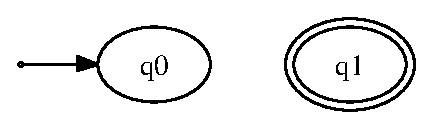
\epsfig{file=Abbildungen/aLeer.eps, scale=0.5}
      \caption{The \textsc{Fsm} $A(\emptyset)$.}
      \label{fig:aLeer.eps}
      \end{figure}
      Figure \ref{fig:aLeer.eps} shows the \textsc{Fsm} $A(\emptyset)$. It is obvious that we have
      $L\bigl(A(\emptyset)\bigr) = \{\}$. 
\item The \textsc{Fsm} $A(\varepsilon)$ is defined as
      \\[0.2cm]
      \hspace*{1.3cm}
      $A(\varepsilon) = \bigl\langle \{ q_0, q_1 \}, \Sigma, 
                          \bigl\{ \pair(q_0, \varepsilon) \mapsto \{q_1\} \bigr\}, q_0, \{ q_1 \} \bigr\rangle$.


      \begin{figure}[!ht]
        \centering
      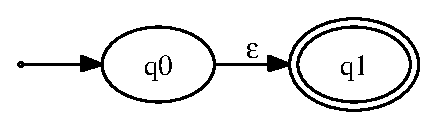
\epsfig{file=Abbildungen/aEpsilon.eps, scale=0.5}
      \caption{The \textsc{Fsm} $A(\varepsilon)$.}
      \label{fig:aEpsilon.eps}
      \end{figure}
      Figure \ref{fig:aEpsilon.eps} shows the \textsc{Fsm} $A(\varepsilon)$.
      We have that $L\bigl(A(\varepsilon)\bigr) = \{\lambda\}$, i.e.~the \textsc{Fsm} accepts only the empty string. 
\item For a letter $c \in \Sigma$ the \textsc{Fsm} $A(c)$ is defined as 
      \\[0.2cm]
      \hspace*{1.3cm}
      $A(c) = \bigl\langle \{ q_0, q_1 \}, \Sigma, 
                                \bigl\{ \langle q_0, c \rangle \mapsto \{q_1\}\bigr\}, q_0, \{ q_1 \} \bigr\rangle$.

      \begin{figure}[!ht]
        \centering
      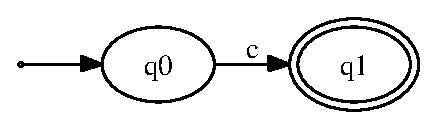
\epsfig{file=Abbildungen/aChar.eps, scale=0.5}
      \caption{The \textsc{Fsm} $A(c)$.}
      \label{fig:aChar.eps}
      \end{figure}
      Figure \ref{fig:aChar.eps} shows $A(c)$.
      We have that $L\bigl(A(c)\bigr) = \{c\}$, i.e.~the \textsc{Fsm} accepts only the character $c$. 
\item In order to define the \textsc{Fsm} $A(r_1 \cdot r_2)$ for the concatenation $r_1 \cdot r_2$ 
      we assume that we have already constructed finite state machines $A(r_1)$ and $A(r_2)$
      such that $L\bigl(A(r_1)\bigr) = L(r_1)$ and $L\bigl(A(r_2)\bigr) = L(r_2)$.  Furthermore,
      without loss of generality we assume that the states in the \textsc{Fsm}s  $A(r_1)$ and $A(r_2)$ are different. 
      This can always be achieved by renaming the states of $A(r_2)$.
      Next, we assume that $A(r_1)$ and $A(r_2)$ have the following form:
      \begin{enumerate}
      \item $A(r_1) = \bigl\langle Q_1, \Sigma, \delta_1, q_1, \{ q_2 \}\bigr\rangle$,
      \item $A(r_2) = \bigl\langle Q_2, \Sigma, \delta_2, q_3, \{ q_4 \}\bigr\rangle$,
      \item $Q_1 \cap Q_2 = \{\}$.
      \end{enumerate}
      Then we can build the \textsc{Fsm} $A(r_1 \cdot r_2)$ from $A(r_1)$ and $A(r_2)$ as follows:
      \\[0.2cm]
      \hspace*{0.8cm}
       $A(r_1 \cdot r_2) := \bigl\langle Q_1 \cup Q_2, \Sigma, 
                \bigl\{ \pair(q_2,\varepsilon) \mapsto \{q_3\} \bigr\} 
                   \cup \delta_1 \cup \delta_2, q_1, \{ q_4 \} \bigr\rangle$
      \\[0.2cm]
      Here, the notation $\{ \pair(q_2,\varepsilon) \mapsto q_3 \} \cup \delta_1 \cup \delta_2$ specifies that
      $A(r_1 \cdot r_2)$ contains all transitions from both $A(r_1)$ and $A(r_2)$ and, furthermore,
      contains an $\varepsilon$-transition from $q_2$ to $q_3$.     
      Formally, this transition function  $\delta$ can be specified as follows:
      \\[0.2cm]
      \hspace*{1.3cm}
      $\delta(q,c) := \left\{
      \begin{array}{ll}
        \{ q_3 \}       & \mbox{if $q = q_2$ and $c = \varepsilon$}, \\[0.2cm]
        \delta_1(q, c)  & \mbox{if $q \in Q_1$ and $\pair(q,c) \not= \pair(q_2,\varepsilon)$}, \\[0.2cm]
        \delta_2(q, c)  & \mbox{if $q \in Q_2$.} 
      \end{array}\right.
      $
      \\[0.2cm]


      \begin{figure}[!ht]
        \centering
      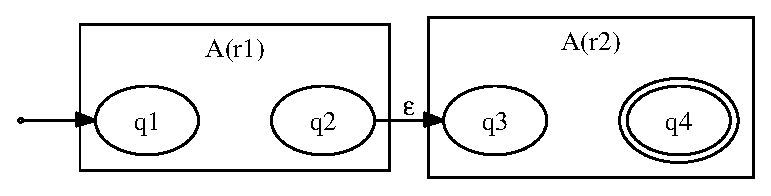
\epsfig{file=Abbildungen/aConcat.eps, scale=0.8}
      \caption{The \textsc{Fsm} $A(r_1 \cdot r_2)$.}
      \label{fig:aConcat.eps}
      \end{figure}
      Figure \ref{fig:aConcat.eps} shows the \textsc{Fsm} $A(r_1 \cdot r_2)$.

      Instead of having an $\varepsilon$-transition from $q_2$ to $q_3$ we can identify the states $q_2$ and
      $q_3$.  The advantage is that the resulting \textsc{Fsm} is smaller.
      We will do this when creating \textsc{Fsm}s by hand.  

      I haven't done this identification in the definition above because both the graphical representation and 
      the implementation get more complicated when we identify these states.
\item In order to define the \textsc{Fsm} $A(r_1 + r_2)$ we assume that we have already constructed finite
      state machines $A(r_1)$ and $A(r_2)$ such that $L\bigl(A(r_1)\bigr) = L(r_1)$ and $L\bigl(A(r_2)\bigr) =
      L(r_2)$.  Furthermore, without loss of generality we assume that the states in the \textsc{Fsm}s
      $A(r_1)$ and $A(r_2)$ are different and that $A(r_1)$ and $A(r_2)$ have the following form:
      \begin{enumerate}
      \item $A(r_1) = \bigl\langle Q_1, \Sigma, \delta_1, q_1, \{ q_3 \}\bigr\rangle$,
      \item $A(r_2) = \bigl\langle Q_2, \Sigma, \delta_2, q_2, \{ q_4 \}\bigr\rangle$,
      \item $Q_1 \cap Q_2 = \{\}$.
      \end{enumerate}
      Then the \textsc{Fsm} $A(r_1 + r_2)$ is defined as follows:
      \\[0.2cm]
      \hspace*{0.8cm}
       $\bigl\langle \{ q_0, q_5 \} \cup Q_1 \cup Q_2, \Sigma, 
                \bigl\{ \pair(q_0,\varepsilon) \mapsto \{q_1, q_2\},
                   \pair(q_3,\varepsilon) \mapsto \{q_5\}, \pair(q_4,\varepsilon) \mapsto \{q_5\} \bigr\} 
                   \cup \delta_1 \cup \delta_2, q_0, \{ q_5 \} \bigr\rangle$

      \begin{figure}[!ht]
        \centering
      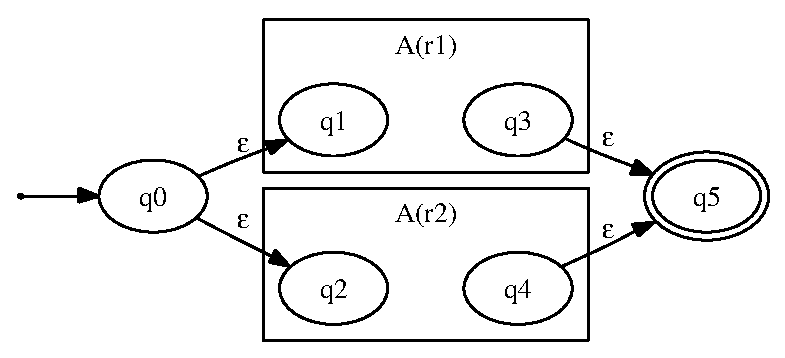
\epsfig{file=Abbildungen/aPlus.eps, scale=0.5}
      \caption{The \textsc{Fsm} $A(r_1 + r_2)$.}
      \label{fig:aPlus.eps}
      \end{figure}
      Figure \ref{fig:aPlus.eps} shows the \textsc{Fsm} $A(r_1 + r_2)$.
      In addition to the states of $A(r_1)$ and $A(r_2)$ there are two more states:
      \begin{enumerate}
      \item $q_0$ is the start state of the \textsc{Fsm} $A(r_1 + r_2)$,
      \item $q_5$ is the only accepting state of the \textsc{Fsm} $A(r_1 + r_2)$.
      \end{enumerate}
      In addition to the transitions of $A(r_1)$ and $A(r_2)$ the \textsc{Fsm} $A(r_1+r_2)$
      has four more $\varepsilon$-transitions.
      \begin{enumerate}
      \item The new start state $q_0$ has two
            $\varepsilon$-transitions leading to the start states $q_1$ and $q_2$ of the \textsc{Fsm}s
            $A(r_1)$ and $A(r_2)$.
      \item Each of the accepting states $q_3$ and $q_4$ of the \textsc{Fsm}s
             $A(r_1)$ and $A(r_2)$ has an $\varepsilon$-transition to the new accepting state $q_5$.
      \end{enumerate}
      In order to simplify this \textsc{Fsm} we could identify the three states
      $q_0$, $q_1$ and $q_2$ and the three states $q_3$, $q_4$ and $q_5$.  However, the resulting \textsc{Fsm}
      would be more difficult to understand and hence we are \underline{\red{not}} doing this when creating 
      \textsc{Fsm}s by hand.
\item In order to define the \textsc{Fsm} $A(r^*)$ we assume that we have already constructed a finite
      state machine $A(r)$ such that $L\bigl(A(r)\bigr) = L(r)$ and that $A(r)$ has the form
      \\[0.2cm]
      \hspace*{1.3cm}
      $A(r) = \bigl\langle Q, \Sigma, \delta, q_1, \{ q_2 \} \bigr\rangle$.
      \\[0.2cm]
      Then  $A(r^*)$ is defined as follows:
      \\[0.2cm]
      \hspace*{0.8cm}
       $\bigl\langle \{ q_0, q_3 \} \cup Q, \Sigma, 
                \bigl\{ \pair(q_0,\varepsilon) \mapsto \{q_1, q_3\}, \pair(q_2,\varepsilon) \mapsto \{q_1, q_3\} \bigr\} 
                \cup \delta, q_0, \{ q_3 \} \bigr\rangle$.
      \\[0.2cm]


      \begin{figure}[!ht]
        \centering
      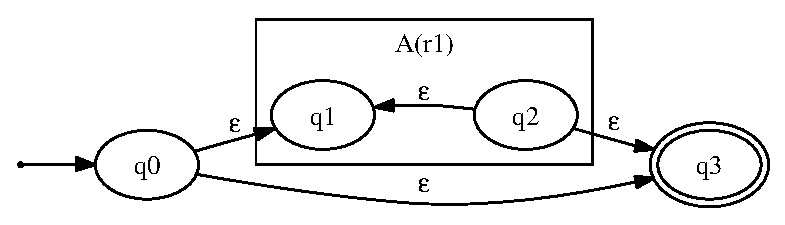
\epsfig{file=Abbildungen/aStar.eps, scale=0.5}
      \caption{The \textsc{Fsm} $A(r^*)$.}
      \label{fig:aStar.eps}
      \end{figure}
      Figure \ref{fig:aStar.eps} shows the \textsc{Fsm} $A(r^*)$.
      In comparison with $A(r)$ this \textsc{Fsm} has two additional states.
      \begin{enumerate}
      \item $q_0$ is the start state of $A(r^*)$,
      \item $q_3$ is the only accepting state of $A(r^*)$.
      \end{enumerate}
      The \textsc{Fsm} $A(r^*)$ has four more $\varepsilon$-transitions than $A(r)$: 
      \begin{enumerate}
      \item The new start state  $q_0$ has $\varepsilon$-transitions to the states
            $q_1$ and $q_3$.
      \item $q_2$ has an $\varepsilon$-transition back to the state $q_1$.
      \item $q_2$ also has an $\varepsilon$-transition to the state $q_3$.
      \end{enumerate}
      \textbf{\textcolor{red}{Attention}}:  If we would identify the two states 
      $q_0$ and $q_1$ and the two states $q_2$ and $q_3$, then the resulting \textsc{Fsm} would no longer be
      correct!
\end{enumerate}

\exerciseEng
Construct a non-deterministic \textsc{Fsm} that accepts the language specified by the regular expression
\\[0.2cm]
\hspace*{1.3cm}
$\texttt{a}^* \cdot \texttt{b}^*$.
\\[0.2cm]
Consider what would happen if you would identify the two states 
$q_0$ and $q_1$ and the two states $q_2$ and $q_3$ in step 6 of the construction given above, while also
identifying the two states $q_2$ and $q_3$ in step 4 of the construction of $A(r_1 \cdot r_2)$.
\eox

\exerciseEng
Construct a non-deterministic \textsc{Fsm} for the regular expression
\\[0.2cm]
\hspace*{1.3cm}
$(\texttt{a} + \texttt{b}) \cdot \texttt{a}^* \cdot \texttt{b}$.  
\eox

\subsection{Implementation}
The \textsl{Jupyter notebook} 
\\[0.2cm]
\hspace*{0.3cm}
\href{https://github.com/karlstroetmann/Formal-Languages/blob/master/Python/Chapter-4/03-Regexp-2-NFA.ipynb}{https://github.com/karlstroetmann/Formal-Languages/blob/master/Python/Chapter-4/03-Regexp-2-NFA.ipynb} 
\\[0.2cm]
implements the theory discussed in this section.



\section{Translating a Deterministic \textsc{Fsm} into a Regular Expression}
In this last section we start with a deterministic \textsc{Fsm} $F$ and construct a regular expression $r$
such that we have
\\[0.2cm]
\hspace*{1.3cm}
$L(r) = L(F)$. 
\\[0.2cm]
We assume that the \textsc{Fsm} $F$ is given as follows:
\\[0.2cm]
\hspace*{1.3cm}
$F = \bigl\langle \{ q_0, q_1, \cdots, q_n \}, \Sigma, \delta, q_0, A \bigr\rangle$.
\\[0.2cm]
For every pair of states $\pair(p_1,p_2) \in Q \times Q$ we define a regular expression
$r(p_1, p_2)$ such that $r(p_1, p_2)$ describes those strings $w$ that take the \textsc{Fsm} $F$ from the state
$p_1$ to the state $p_2$, i.e.~we have
\\[0.2cm]
\hspace*{1.3cm}
$L\bigl(r(p_1, p_2)\bigr) = 
  \bigl\{ w \in \Sigma^* \mid \pair(p_1,w) \leadsto^* \pair(p_2, \varepsilon) \bigr\}$.
\\[0.2cm]  
The definition of $r(p_1, p_2)$ is done by first defining auxiliary regular expressions 
$r^{(k)}(p_1, p_2)$ for all $k =0,\cdots,n+1$.   The regular expression $r^{(k)}(p_1, p_2)$ specifies those
strings that take the \textsc{Fsm} $F$ from the state
$p_1$ to the state $p_2$ without visiting a state from the set
\\[0.2cm]
\hspace*{1.3cm}
$Q_k := \bigl\{ q_i \mid i \in \{k,\cdots,n \}  \bigl\} = \{ q_k, \cdots, q_n \}$.
\\[0.2cm]
To this end we define the ternary relation
\\[0.2cm]
\hspace*{1.3cm}
$\mapsto_k \;\subseteq\; (Q \times \Sigma^* \times Q)$.
\\[0.2cm]
Given two states $p, q \in Q$ and a string $w$ we have that
\\[0.2cm]
\hspace*{1.3cm}
$p \stackrel{w}{\mapsto}_k q$
\\[0.2cm]
holds iff the \textsc{Fsm} $F$ switches from the state $p$ to the state $q$ when it reads the string $w$
but on reading $w$ does not switch to a state from the set
$Q_k$ \blue{in-between}.  Here, ``in-between'' specifies that the states $p$ and $q$ may well be elements of the set
$Q_k$, only the states between $p$ and $q$ must not be in $Q_k$.
The formal definition of $p \stackrel{w}{\mapsto}_k q$ is done by induction on  $w$:
\begin{enumerate}
\item[B.C.:] $|w| \leq 1$.  Then there are two cases:
  \begin{enumerate}
  \item $p \stackrel{\varepsilon}{\mapsto}_k p$,

        because when the empty string is read we can only reach the state $p$ if we start in the state $p$.
  \item $\delta(p, c) = q \;\Rightarrow\; p \stackrel{c}{\mapsto}_k q$,

        because when the \textsc{Fsm} reads the character $c$ and switches from state $p$ directly
        to the state $q$, there are no states ``inbetween''.
  \end{enumerate}
\item[I.S.:] $w = cv$ where $|v| \geq 1$.

             Here we have:
             \hspace*{1.3cm}
            $p \stackrel{c}{\mapsto} q \wedge q \not\in Q_k \wedge q \stackrel{v}{\mapsto}_k r
              \;\Rightarrow\; p \stackrel{cv}{\mapsto}_k r$.
\end{enumerate}
Now we are ready to define the regular expressions $r^{(k)}(p_1, p_2)$ for all $k=0,\cdots,n+1$.
This definition will be done such that we have
\\[0.2cm]
\hspace*{1.3cm}
$L\bigl(r^{(k)}(p_1, p_2)\bigr) = \bigl\{ w \in \Sigma^* \mid p_1 \stackrel{w}{\mapsto}_k p_2 \bigr\}$.
\\[0.2cm]
The definition of the regular expressions $r^{(k)}(p_1, p_2)$ is done by induction on $k$.
\begin{enumerate}
\item[B.C.:] $k = 0$.  

  Then we have $Q_0 = Q$ and therefore the set $Q_0$ contains all states.
  Therefore, when the \textsc{Fsm} switches from the state $p_1$ to the state $p_2$ it must not visit any
  states in-between.  There are two cases.
  \begin{enumerate}
  \item $p_1 \not= p_2$:  Then we can have  $p_1 \stackrel{w}{\mapsto}_0 p_2$ only if $w$ contains but a
        single letter.  Define
        \\[0.2cm]
        \hspace*{1.3cm}
        $\{ c_1, \cdots, c_l \} := \{ c \in \Sigma \mid \delta(p_1,c) = p_2 \}$
        \\[0.2cm]
        as the set of all letters that take the \textsc{Fsm} from the state $p_1$ to the state $p_2$.
        If this set is not empty we define 
        \\[0.2cm]
        \hspace*{1.3cm}
        $r^{(0)}(p_1, p_2) := c_1 + \cdots + c_l$. 
        \\[0.2cm]
        If this set is empty, then there is no direct transition from  $p_1$ to $p_2$ and we define
        \\[0.2cm]
        \hspace*{1.3cm}
        $r^{(0)}(p_1, p_2) := \emptyset$.
  \item $p_1 = p_2$:  Again we define
        \\[0.2cm]
        \hspace*{1.3cm}
        $\{ c_1, \cdots, c_l \} := \{ c \in \Sigma \mid \delta(p_1,c) = p_1 \}$.
        \\[0.2cm]
        If this set is not empty we have
        \\[0.2cm]
        \hspace*{1.3cm}
        $r^{(0)}(p_1, p_1) := c_1 + \cdots + c_l + \varepsilon$.
        \\[0.2cm]
        Otherwise we have
        \\[0.2cm]
        \hspace*{1.3cm}
        $r^{(0)}(p_1, p_1) := \varepsilon$.
   \end{enumerate}
\item[I.S.:] $k \mapsto k+1$.  

  When compared to the regular expression $r^{(k)}(p_1, p_2)$,
  the regular expression  $r^{(k+1)}(p_1, p_2)$ is allowed to use the state
  $q_k$, because $q_k$ is the only element of the set $Q_k$ that is not a member of the set $Q_{k+1}$.  
  If the \textsc{Fsm} reads a string $w$ that switches the state $p_1$ to the state $p_2$ without switching into a state
  from the set $Q_{k+1}$, then there are two cases.
  \begin{enumerate}
  \item We already have $p_1 \stackrel{w}{\mapsto}_k p_2$.
  \item The string $w$ can be written as  $w = w_1 s_1\cdots s_l w_2$ where we have:
        \begin{itemize}
        \item $p_1 \stackrel{w_1}{\mapsto}_k q_k$,
        \item $q_k \stackrel{s_i}{\mapsto}_k q_k$ \quad for all $i = \{ 1, \cdots, l\}$,
        \item $q_k \stackrel{w_2}{\mapsto}_k p_2$.
        \end{itemize}
        Therefore we define
        \\[0.2cm]
        \hspace*{1.3cm}
        $r^{(k+1)}(p_1,p_2) := 
         r^{(k)}(p_1,p_2) + 
         r^{(k)}(p_1,q_k) \cdot \bigl(r^{(k)}(q_k,q_k)\bigr)^* \cdot r^{(k)}(q_k,p_2)$.
  \end{enumerate}  
\end{enumerate}
Now we are ready to define the regular expressions $r(p_1,p_2)$ for all states $p_1$ and $p_2$:
\\[0.2cm]
\hspace*{1.3cm}
$r(p_1,p_2) := r^{(n+1)}(p_1,p_2)$. 
\\[0.2cm]
This regular expression specifies all strings that take the \textsc{Fsm} from the state
$p_1$ to the state $p_2$ without using any state from the set 
$Q_{n+1}$ in-between.   Since we have
\\[0.2cm]
\hspace*{1.3cm}
$Q_{n+1} = \bigl\{ q_i \mid i \in \{0,\cdots,n \} \wedge i \geq n+1 \bigr\} = \{\}$
\\[0.2cm]
we know that $Q_{n+1}$ is empty.
Therefore the regular expression $r^{(n+1)}(p_1,p_2)$
does not exclude any states when switching from
state $p_1$ to the state $p_2$.

In order to construct a regular expression that specifies the language accepted by a deterministic \textsc{Fsm}
$F$ we write the set $A$ of accepting states of $F$ as
\\[0.2cm]
\hspace*{1.3cm}
$A = \{ t_1, \cdots, t_m \}$.
\\[0.2cm]
Then the regular expression $r(A)$ is defined as
\\[0.2cm]
\hspace*{1.3cm}
$r(A) := r(q_0, t_1) + \cdots + r(q_0, t_m)$.
\\[0.2cm]
This regular expression specifies those strings that take the \textsc{Fsm} $F$ from its start state $q_0$ into
any of its accepting states.
\qed


\exerciseEng
Take the \textsc{Fsm} shown in Figure \ref{fig:abstara.dot} and construct an equivalent regular expression.


\solutionEng
The \textsc{Fsm} has two states: $0$ and $1$.  We start by computing the regular expressions
$r^{(k)}(i,j)$ for all $i,j\in\{0,1\}$ for  $k =0$, $1$, and $2$:
\begin{enumerate}
\item For $k = 0$ we have:
      \begin{enumerate}
      \item $r^{(0)}(0, 0) = \texttt{a} + \varepsilon$,
      \item $r^{(0)}(0, 1) = \texttt{b}$,
      \item $r^{(0)}(1, 0) = \emptyset$,
      \item $r^{(0)}(1, 1) = \texttt{a} + \varepsilon$.
      \end{enumerate}
\item For $k=1$ we have:
      \begin{enumerate}
      \item For $r^{(1)}(0, 0)$ we have:
            \begin{eqnarray*}
                  r^{(1)}(0, 0) 
            & = & r^{(0)}(0, 0) + 
                  r^{(0)}(0, 0) \cdot \bigl(r^{(0)}(0, 0)\bigr)^* \cdot r^{(0)}(0, 0) \\
            & \doteq & r^{(0)}(0, 0) \cdot \bigl(r^{(0)}(0, 0)\bigr)^*
            \end{eqnarray*}
             In the last step we used the fact that 
             \\[0.2cm]
             \hspace*{1.3cm}
             $
             \begin{array}[t]{lcl}
               r + r \cdot r^* \cdot r & \doteq & r \cdot (\varepsilon + r^* \cdot r) \\
                                       & \doteq & r \cdot r^*
             \end{array}
             $
             \\[0.2cm]
             to simplify the result.
             If we substitute for $r^{(0)}(0, 0)$ the expression $\texttt{a} + \varepsilon$  
             we get 
             \\[0.2cm]
             \hspace*{1.3cm}
             $r^{(1)}(0, 0) \doteq (\texttt{a} + \varepsilon)\cdot (\texttt{a} + \varepsilon)^*$.
             \\[0.2cm]
             As we have $(\texttt{a} + \varepsilon)\cdot (\texttt{a} + \varepsilon)^* \doteq \texttt{a}^*$ we have
             \\[0.2cm]
             \hspace*{1.3cm}
             $r^{(1)}(0, 0) \doteq \texttt{a}^*$.
      \item For $r^{(1)}(0, 1)$ we have:
            \begin{eqnarray*}
                  r^{(1)}(0, 1) 
            & \doteq & r^{(0)}(0, 1) + 
                  r^{(0)}(0, 0) \cdot \bigl(r^{(0)}(0, 0)\bigr)^* \cdot r^{(0)}(0, 1) \\
            & \doteq & \texttt{b} + 
                  (\texttt{a} + \varepsilon) \cdot (\texttt{a} + \varepsilon)^* \cdot \texttt{b} \\
            & \doteq & \texttt{b} + \texttt{a}^* \cdot \texttt{b} \\
            & \doteq & (\varepsilon + \texttt{a}^*) \cdot \texttt{b} \\
            & \doteq & \texttt{a}^* \cdot \texttt{b} 
        \end{eqnarray*}
      \item For $r^{(1)}(1, 0)$ we have:
            \begin{eqnarray*}
                  r^{(1)}(1, 0) 
            & \doteq & r^{(0)}(1, 0) + 
                  r^{(0)}(1, 0) \cdot \bigl(r^{(0)}(0, 0)\bigr)^* \cdot r^{(0)}(0, 0) \\
            & \doteq & \emptyset + \emptyset \cdot (\texttt{a} + \varepsilon)^* \cdot (\texttt{a} + \varepsilon) \\
            & \doteq & \emptyset
            \end{eqnarray*}
      \item For $r^{(1)}(1, 1)$ we have
            \begin{eqnarray*}
                  r^{(1)}(1, 1)
            & \doteq & r^{(0)}(1, 1) + 
                  r^{(0)}(1, 0) \cdot \bigl(r^{(0)}(0, 0)\bigr)^* \cdot r^{(0)}(0, 1) \\
            & \doteq & (\texttt{a} + \varepsilon) + 
                  \emptyset \cdot (\texttt{a} + \varepsilon)^* \cdot \texttt{b} \\
            & \doteq & (\texttt{a} + \varepsilon) + \emptyset  \\
            & \doteq & \texttt{a} + \varepsilon  
            \end{eqnarray*}
      \end{enumerate}
\item For $k=2$ we only have to compute the regular expression $r^{(2)}(0, 1)$:
            \begin{eqnarray*}
                  r^{(2)}(0, 1)
            & \doteq & r^{(1)}(0, 1) + 
                  r^{(1)}(0, 1) \cdot \bigl(r^{(1)}(1, 1)\bigr)^* \cdot r^{(1)}(1, 1) \\
            & \doteq & \texttt{a}^* \cdot \texttt{b} + 
                  \texttt{a}^* \cdot \texttt{b} \cdot (\texttt{a} + \varepsilon)^* \cdot (\texttt{a} + \varepsilon) \\
            & \doteq & \texttt{a}^* \cdot \texttt{b} + \texttt{a}^* \cdot \texttt{b} \cdot \texttt{a}^* \\
            & \doteq & \texttt{a}^* \cdot \texttt{b} \cdot (\varepsilon + \texttt{a}^*) \\
            & \doteq & \texttt{a}^* \cdot \texttt{b} \cdot \texttt{a}^*.
        \end{eqnarray*}
\end{enumerate}
As the state 0 is the start state and the state $1$ is the only accepting state we have
\\[0.2cm]
\hspace*{1.3cm}
$r(F) = r^{(2)}(0, 1) \doteq \texttt{a}^* \cdot \texttt{b} \cdot \texttt{a}^*$.
\qed


\exerciseEng
Take the \textsc{Fsm} shown in Figure \ref{fig:exercise-13.eps} on page
\pageref{fig:exercise-13.eps} and construct a regular expression specifying the same language as this
\textsc{Fsm}.
\vspace*{0.1cm}

\noindent
\textbf{Hint}: In order to avoid unnecessary computations, you should only compute those regular expression
$r^{(k)}(p, q)$ that are needed in order to compute $r^{(3)}(q_0, q_2)$. 
\eox

\begin{figure}[!ht]
  \centering
\epsfig{file=Abbildungen/exercise-13.eps, scale=1.0}
\caption{A deterministic finite state machine.}
\label{fig:exercise-13.eps}
\end{figure}

\subsection{Implementation}
The \textsl{Jupyter notebook} 
\\[0.2cm]
\hspace*{1.3cm}
\href{https://github.com/karlstroetmann/Formal-Languages/blob/master/Python/05-DFA-2-RegExp.ipynb}{https://github.com/karlstroetmann/Formal-Languages/blob/master/Python/05-DFA-2-RegExp.ipynb}
\\[0.2cm]
contains a program that takes a deterministic \textsc{Fsm} $F$ and computes a regular expression $r$ such that
$r$ specifies the language accepted by $F$, i.e.~we have $L(r) = L(F)$.

\section{Minimization of Finite State Machines}
In this section we show how to minimize the number of states of a deterministic finite state machine
\\[0.2cm]
\hspace*{1.3cm}
$F = \langle Q, \Sigma, \delta, q_0, A \rangle$.
\\[0.2cm]
Without loss of generality we want to assume that the \textsc{Fsm} $F$ is complete: Therefore, we assume that
for each state $q \in Q$ and each letter $c \in \Sigma$ the expression $\delta(q, c)$ 
returns a state of $Q$.  Our goal is to find a deterministic finite state machine
\\[0.2cm]
\hspace*{1.3cm}
$F^- = \langle Q^-, \Sigma, \delta^-, q_0, A^- \rangle$,
\\[0.2cm]
which accepts the same language as  $F$, so 
\\[0.2cm]
\hspace*{1.3cm}
$L(F^-) = L(F)$
\\[0.2cm]
and for which the number of states of the set $Q^-$ is minimal.  
We start with the function 
\\[0.2cm]
\hspace*{1.3cm}
$\delta^*: Q \times \Sigma^* \rightarrow Q$
\\[0.2cm]
which extends the function $\delta$ by accepting a string instead of a single character as its first argument.
The function call $\delta^*(q,s)$ calculates the state $p$ which the \textsc{Fsm} $F$ enters if it reads the
string $s$ in the state $q$. As we have assumed the \textsl{Fsm} F to be complete, we have that
\\[0.2cm]
\hspace*{1.3cm}
$\delta(q, c) \not\in \Omega$ \quad for all $q \in Q$ and all $c \in \Sigma$ 
\\[0.2cm]
and then $\delta^*(q,w)$ is defined by induction on $w$ as follows:
\begin{enumerate}[(a)]
\item $\delta^*(q, \varepsilon) := q$ \quad for all $q \in Q$.
\item $\delta^*(q, cw) := \delta^*(\delta(q, c), v)$ \quad for all $q \in Q$, $c \in \Sigma$, and $v \in \Sigma^*$.
\end{enumerate}
Since the function $\delta^*$ is a generalization of the function $\delta$, in
the future we will not distinguish in the notation between $\delta$ and $\delta^*$ and write $\delta$ for both functions. 

Obviously, in a finite state machine 
$F = \langle Q, \Sigma, \delta, q_0, A \rangle$ we can remove all the states $p \in Q$ which are not
\blue{reachable} from the start state.  A state $p$ is \blue{reachable}\index{reachable} iff 
a string $w \in \Sigma^*$ is given, such that
\\[0.2cm]
\hspace*{1.3cm}
$\delta(q_0, w) = p$
\\[0.2cm]
holds.  In the following we assume that all states of the \textsc{Fsm} $F$ can be reached
from the start state. 


\begin{figure}[!ht]
  \centering
  \epsfig{file=Abbildungen/nicht-gleichwertig.eps, scale=0.6}
   \caption{A finite state machine with equivalent states.}
  \label{fig:nicht-gleichwertig.dot}
\end{figure}

In general, we can minimize an \textsc{Fsm} by identifying certain states.   
If we look for example at the \textsc{Fsm} shown in figure \ref{fig:nicht-gleichwertig.dot}, we can identify
the states $q_1$ and $q_2$ as well as $q_3$ and $q_4$ without changing the language of the \textsc{Fsm}. 
The central idea in minimizing a \textsc{Fsm} is that we compute those states which \textbf{must not} be
identified and consider all other states as equivalent.  States that must not be identified are called
\blue{separable states}.  This notion is defined next.

\begin{Definition}[Separable States]
Assume $F = \langle Q, \Sigma, \delta, q_0, A \rangle$ is a deterministic finite state machine.
Two states $p_1,p_2 \in Q$ are called \blue{separable} \index{separable} if and only if there exists a string 
$s \in \Sigma^*$ such that either
\begin{enumerate}
\item $\delta(p_1,s) \in    A$ and $\delta(p_2,s) \notin A$ or
\item $\delta(p_1,s) \notin A$ and $\delta(p_2,s) \in    A$
\end{enumerate}
holds.  In this case, the string $s$ \blue{separates} \index{separates} $p_1$ and $p_2$. \qed
\end{Definition}
If two states $p_1$ and $p_2$ are separable, then it is obvious that theses states must not be identified.
We define an equivalence relation $\sim$ on the set $Q$ of all states by setting
\\[0.2cm]
\hspace*{1.3cm}
$p_1 \sim p_2$ \quad iff \quad 
$\forall s \in \Sigma^*:\bigl(\delta(p_1,s) \in A \leftrightarrow \delta(p_2,s) \in A\bigr)$.
\\[0.2cm]
Hence, two states $p_1$ and $p_2$ are considered to be equivalent iff they are not separable.   
The claim is that we can identify all pairs $\langle p_1, p_2\rangle$ of equivalent states.  The
\blue{identification} \index{identification of states} 
of two states $p_1$ and $p_2$ is done by removing the state $p_2$ from the set $Q$ and changing the transition
function $\delta$ in a way that the new version of $\delta$ will return $p_1$ in all those cases where the old
version of $\delta$ had returned $p_2$. 


The question remains how we can determine which states are distinguishable.
One possibility is to create a set $V$ with pairs of states.  We add the pair $\langle p, q \rangle$ to the set
$V$ if we have discovered that $p$ and $q$ are distinguishable.  We recognize $p$ and $q$ as distinguishable if
there is a letter $c\in\Sigma$ and two states $s$ and $t$ that are already known to be distinguishable such that 
\\[0.2cm]
\hspace*{1.3cm}
$\delta(p,c) = s$, \quad $\delta(q,c) = t$, \quad and \quad $\langle s, t \rangle \in V$
\\[0.2cm]
holds. This idea leads to an algorithm that uses two steps:
\begin{enumerate}[(a)]
\item First we initialize $V$ with all the pairs $\pair(p,q)$, for which either $p$ is an accepting state and
      $q$ is not an accepting state, or $q$ is an accepting state and $p$ is not an accepting state,
      because an accepting state can be distinguished from a non-accepting state by the empty string
      $\lambda$: 
      \\[0.2cm]
      \hspace*{1.3cm}
      $V := \bigl\{\pair(p,q) \in Q \times Q \mid (p \in A \wedge q \notin A) \vee 
      (p \notin A \wedge q \in A) \bigr\}$
      \\[0.2cm]
      This can also be written as the union of two Cartesian products. We have
      \\[0.2cm]
      \hspace*{1.3cm}
      $V = A \times (Q \backslash A) \cup (Q \backslash A) \times A$.
\item As long as we find a new pair $\pair(p,q) \in Q \times Q$ for which there is a letter $c$ such that the
      states $\delta(p,c)$ and $\delta(q,c)$ are already distinguishable, we add this pair to the set $V$:  
      \\[0.2cm]
      \hspace*{1.3cm} 
      \texttt{while $\exists \pair(p,q) \in Q \times Q: \exists c \in \Sigma:\langle\delta(p,c),
        \delta(q,c)\rangle \in V \wedge \pair(p,q) \notin V$ } \\
      \hspace*{1.8cm}
      \texttt{choose $\pair(p,q) \in Q \times Q$ such that} $\langle\delta(p,c),
      \delta(q,c)\rangle \in V \wedge \pair(p,q) \notin V$ \\
      \hspace*{2.3cm}
      \texttt{$V$ := $V \cup \{\, \pair(p,q),\, \pair(q,p)\, \}$;} \\
\end{enumerate}
If we have found all pairs $\pair(p,q)$ of distinguishable states, then we can identify all states $p$ and $q$
which are not distinguishable and therefore $\langle p, q \rangle \not\in V$.   The \textsc{Fsm} constructed in
this way is, in fact, minimal.  

\exerciseEng
We consider the  \textsc{Fsm} shown in figure \ref{fig:nicht-gleichwertig.dot} and apply the algorithm
described above to this \textsc{Fsm}. 
We use a table for this.  The columns and rows of this table are numbered with the different states.  If we
have recognized in the first step that the states $i$ and $j$ are distinguishable, we insert a $1$ in this
table in the $i$-th row and the $j$-th column. 
Furthermore, since the states $i$ and $j$ can also be distinguished from the states $j$ and $i$, we also insert
a $1$ in the $j$-th row and the $i$-th column. 
\begin{enumerate}
\item In the first step we recognize that the two accepting states $q_3$ and $q_4$ are distinguishable from all non-accepting states.
      So the pairs 
      $\pair(q_0,q_3)$,
      $\pair(q_0,q_4)$,
      $\pair(q_1,q_3)$,
      $\pair(q_1,q_4)$,
      $\pair(q_2,q_3)$ and
      $\pair(q_2,q_4)$
      are distinguishable. So the table now has the following configuration:
      \begin{center}        
      \begin{tabular}[t]{|l||l|l|l|l|l|}
      \hline
            & $q_0$    &    $q_1$ &    $q_2$ &      $q_3$ &      $q_4$  \\
      \hline
      \hline
      $q_0$ &          &          &          & $1$ & $1$  \\
      \hline
      $q_1$ &          &          &          &$1$ &$1$  \\
      \hline
      $q_2$ &          &          &          &$1$ &$1$  \\
      \hline
      $q_3$ &$1$        &$1$         &       $1$ &          &           \\
      \hline
      $q_4$ &$1$ &$1$ &$1$ &          &           \\
      \hline
      \end{tabular}
      \end{center}
\item Next we see that the states $q_0$ and $q_1$ are distinguishable because
      \\[0.2cm]
      \hspace*{1.3cm}
      $\delta(q_0,a) = q_1$, \quad $\delta(q_1,a) = q_3$ \quad and \quad $q_1 \not\sim q_3$.
      \\[0.2cm]
      Also we see that the states $q_0$ and $q_2$ are distinguishable, because
      \\[0.2cm]
      \hspace*{1.3cm}
      $\delta(q_0,b) = q_2$, \quad $\delta(q_2,b) = q_4$ \quad and \quad $q_2 \not\sim q_4$.
      \\[0.2cm]
      Since we have found in the second step that $q_0 \not\sim q_1$ and $q_0 \not\sim q_2$ holds true, we will insert a $2$ at the corresponding positions in the table. Therefore the table now has the following form:
      \begin{center}        
      \begin{tabular}[t]{|l||l|l|l|l|l|}
      \hline
        & $q_0$      &      $q_1$ &      $q_2$ &      $q_3$ &      $q_4$  \\
      \hline
      \hline
      $q_0$ &          &$2$ &$2$ &$1$ &$1$  \\
      \hline
      $q_1$ &$2$ &          &          &$1$ &$1$  \\
      \hline
      $q_2$ &$2$ &          &          &$1$ &$1$  \\
      \hline
      $q_3$ &$1$ &$1$ &$1$ &          &           \\
      \hline
      $q_4$ &$1$ &$1$ &$1$ &          &           \\
      \hline
      \end{tabular}
      \end{center}
\item Now we do not find any more pairs of distinguishable states, because if we take a look at the pair $\pair(q_1,q_2)$ we can see that
      \\[0.2cm]
      \hspace*{1.3cm}
      $\delta(q_1,\texttt{a}) = q_3$ \quad and \quad $\delta(q_2,\texttt{a}) = q_4$, 
      \\[0.2cm]
      but because the states $q_3$ and $q_4$ are not distinguishable so far, this does not yield a new
      distinguishable pair.  Neither does 
      \\[0.2cm]
      \hspace*{1.3cm}
      $\delta(q_1,\texttt{b}) = q_3$ \quad and \quad $\delta(q_2,\texttt{b}) = q_4$
      \\[0.2cm]
      yield a new distinguishable pair.  At this point, the two states $q_3$ and $q_4$ remain.  We find
      \\[0.2cm]
      \hspace*{1.3cm}
      $\delta(q_3,c) = q_1$ \quad and \quad $\delta(q_4,c) = q_2$ \quad for all $c \in \{\texttt{a}, \texttt{b}\}$
      \\[0.2cm]
      and because the states $q_1$ and $q_2$ are not yet known to be distinguishable, we have not found any new distinguishable states.
      So we can read the equivalent states from the table, it holds that:
      \begin{enumerate}
      \item $q_1 \sim q_2$
      \item $q_3 \sim q_4$
      \end{enumerate}
      Figure \ref{fig:gleichwertig.dot} shows the corresponding reduced finite \textsc{Fsm}.
\end{enumerate}


\begin{figure}[!ht]
  \centering
  \epsfig{file=Abbildungen/gleichwertig.eps, scale=0.6}
   \caption{The reduced \textsc{Fsm}.}
  \label{fig:gleichwertig.dot}
\end{figure}



\exerciseEng
Construct the minimal deterministic  \textsc{Fsm} that recognizes the language 
$L\bigl(a \cdot (b \cdot a)^*\bigr)$.  Perform the following steps:
\begin{enumerate}[(a)]
\item Construct a non-deterministic \textsc{Fsm} which recognizes this language.
\item Transform this non-deterministic \textsc{Fsm} into a deterministic \textsc{Fsm}.
\item Minimize the number of states of this \textsc{Fsm} with the algorithm given above.
\end{enumerate}

\subsection{Implementation}
The \textsl{Jupyter notebook} 
\\[0.2cm]
\hspace*{1.3cm}
\href{https://github.com/karlstroetmann/Formal-Languages/blob/master/Python/DFA-2-RegExp.ipynb}{https://github.com/karlstroetmann/Formal-Languages/blob/master/Python/Minimize.ipynb}
\\[0.2cm]
contains a program that takes a deterministic \textsc{Fsm} $F$ and returns an equivalent \textsc{Fsm} that has
the minimum number of states.


\section{Conclusion}
In this chapter we have shown that the concept of a \blue{deterministic finite state machine}
and a \blue{regular expression} are equivalent.
\begin{enumerate}[(a)]
\item Every deterministic finite state machine can be translated into an equivalent regular expression.
\item Every regular expression can be translated into an equivalent non-deterministic \textsc{Fsm}.
\item Every non-deterministic \textsc{Fsm} can be transformed into an equivalent
      deterministic \textsc{Fsm}.
\end{enumerate}
Furthermore, we have shown that every deterministic finite state machine can be minimized.

\paragraph{Historical Remark}
\href{http://en.wikipedia.org/wiki/Stephen_Cole_Kleene}{Stephen C.~Kleene} (1909 -- 1994) has shown in 1956 that the concepts of 
\blue{finite state  machines} and \blue{regular expression} have the same strength
\cite{kleene:1956}.
\pagebreak

\section{Check your Understanding}
\begin{enumerate}[(a)]
\item How are deterministic and non-deterministic finite state machines defined?
\item Given a non-deterministic \textsc{Fsm} $F$, can you convert it into a deterministic \textsc{Fsm}
      $\mathtt{det}(F)$ that accepts the same language as the \textsc{Fsm} $F$?
\item Given a regular expression $r$, can you describe the steps necessary to construct a non-deterministic
      \textsc{Fsm} $F$ that accepts the language specified by $r$?
\item Given a deterministic \textsc{Fsm} $F$ can you describe how to construct a regular expression $r$
      that specifies the language accepted by $F$?
\item How do we mimimize a finite state machine?
\end{enumerate}

%%% Local Variables: 
%%% mode: latex
%%% TeX-master: "formal-languages.tex"
%%% End: 

%\chapter[Minimierung von FSMs$^*$]{Minimierung endlicher Automaten$^*$}
In diesem Abschnitt zeigen wir ein Verfahren, mit dem die Anzahl der Zust\"ande eines deterministischen
endlichen Automaten 
\\[0.2cm]
\hspace*{1.3cm}
$A = \langle Q, \Sigma, \delta, q_0, F \rangle$
\\[0.2cm]
minimiert werden kann.  Ohne Beschr\"ankung der Allgemeinheit wollen wir dabei voraussetzen,
dass der Automat $A$ vollst\"andig ist: Wir nehmen also an, dass der Ausdruck $\delta(q, c)$
f\"ur jeden Zustand $q \in Q$ und jeden Buchstaben $c \in \Sigma$ als Ergebnis einen Zustand
aus $Q$ liefert. Wir suchen dann einen deterministischen
endlichen Automaten 
\\[0.2cm]
\hspace*{1.3cm}
$A^- = \langle Q^-, \Sigma, \delta^-, q_0, F^- \rangle$,
\\[0.2cm]
der dieselbe Sprache akzeptiert wie der Automat $A$, f\"ur den also
\\[0.2cm]
\hspace*{1.3cm}
$L(A^-) = L(A)$
\\[0.2cm]
gilt und f\"ur den die Anzahl der Zust\"ande der Menge $Q^-$ minimal ist.  
Um diese
Konstruktion durchf\"uhren zu k\"onnen, m\"ussen wir etwas ausholen.
Zun\"achst erweitern wir die Funktion 
\\[0.2cm]
\hspace*{1.3cm}
$\delta: Q \times \Sigma \rightarrow Q$
\\[0.2cm]
zu einer Funktion $\hat{\delta}$, die als zweites Argument nicht nur einen Buchstaben
sondern auch einen String akzeptiert:
\\[0.2cm]
\hspace*{1.3cm}
$\hat{\delta} : Q \times \Sigma^* \rightarrow Q$.
\\[0.2cm]
Der Funktions-Aufruf $\hat{\delta}(q,s)$ soll den Zustand $p$ berechnen, in den der Automat $A$ gelangt,
wenn der Automat im Zustand $q$ den String $s$ liest.
Die Definition von $\hat{\delta}(q,s)$ erfolgt durch Induktion \"uber die L\"ange des Strings $s$:
\begin{enumerate}
\item[I.A.:] $\hat{\delta}(q,\varepsilon) = q$,
\item[I.S.:] $\hat{\delta}(q,cs) = \hat{\delta}\bigl(\delta(q,c),s\bigr)$, 
             falls $c \in   \Sigma$ und $s \in \Sigma^*$.
\end{enumerate}
Da die Funktion $\hat{\delta}$ eine Verallgemeinerung der Funktion $\delta$ ist, werden wir in der
Notation nicht zwischen $\delta$ und $\hat{\delta}$ unterscheiden und einfach nur $\delta$ schreiben.

Offensichtlich k\"onnen wir in einem endlichen Automaten 
$A = \langle Q, \Sigma, \delta, q_0, F \rangle$  alle die Zust\"ande $p \in Q$ entfernen,
die vom Start-Zustand aus nicht 
\emph{erreichbar} sind.  Dabei hei{\ss}t ein Zustand $p$ \emph{erreichbar} genau dann, wenn es
einen String $w \in \Sigma^*$ gibt, so dass
\\[0.2cm]
\hspace*{1.3cm}
$\delta(q_0, w) = p$
\\[0.2cm]
gilt.  Wir wollen im Folgenden daher voraussetzen, dass alle Zust\"ande des betrachteten
endlichen Automaten vom Start-Zustand aus erreichbar sind.


\begin{figure}[!ht]
  \centering
  \epsfig{file=Abbildungen/nicht-gleichwertig.eps, scale=0.6}
   \caption{Ein endlicher Automat mit \"aquivalenten Zust\"anden.}
  \label{fig:nicht-gleichwertig.dot}
\end{figure}

Im Allgemeinen k\"onnen wir einen Automaten dadurch minimieren, dass wir bestimmte Zust\"ande
identifizieren.  Betrachten wir beispielsweise den in Abbildung
\ref{fig:nicht-gleichwertig.dot} gezeigten Automaten, so k\"onnen wir dort die Zust\"ande $q_1$
und $q_2$ sowie $q_3$ und $q_4$ identifizieren, ohne dass sich dadurch die Sprache des
Automaten \"andert.  
Die zentrale Idee bei der Minimierung eines Automaten besteht darin, dass wir uns
\"uberlegen, welche Zust\"ande wir auf keinen Fall identifizieren d\"urfen und einfach alle
anderen Zust\"ande als \"aquivalent betrachten.

\begin{Definition}[Separable States]
Assume $A = \langle Q, \Sigma, \delta, q_0, F \rangle$ is a deterministic finite state machine.
Two states $p_1,p_2 \in Q$ are called \emph{separable} if and only if there exists a string 
$s \in \Sigma^*$ such that either
\begin{enumerate}
\item $\delta(p_1,s) \in    F$ and $\delta(p_2,s) \notin F$ or
\item $\delta(p_1,s) \notin F$ and $\delta(p_2,s) \in    F$
\end{enumerate}
holds.  In this case, the string $s$ \emph{separates} $p_1$ and $p_2$. \qed
\end{Definition}
If two states $p_1$ and $p_2$ are separable, then it is obvious that theses states are not
equivalent.
We define an equivalence relation $\sim$ on the set $Q$ of all states by setting
\\[0.2cm]
\hspace*{1.3cm}
$p_1 \sim p_2$ \quad iff \quad 
$\forall s \in \Sigma^*:\bigl(\delta(p_1,s) \in F \leftrightarrow \delta(p_2,s) \in F\bigr)$.
\\[0.2cm]
Hence, two states $p_1$ and $p_2$ are considered to be equivalent iff they are not separable.   
The claim is that we can identify all equivalent states.  The identification of two states $p_1$ and
$p_2$ is done by removing the state $p_2$ from the set $Q$ and changing the transition
function $\delta$ in a way that the new version of $\delta$ will return
$p_1$ in all those cases where the old version of $\delta$ had returned $p_2$.


Es bleibt die Frage zu kl\"aren, wie wir feststellen k\"onnen, welche Zust\"ande unterscheidbar sind.
Eine M\"oglichkeit besteht darin, eine Menge $V$ von Paaren von Zust\"ande anzulegen.  Wir f\"ugen
das Paar $\langle p, q \rangle$ in die Menge $V$ ein, wenn wir erkannt haben, dass $p$ und $q$
unterscheidbar sind.  Wir erkennen $p$ und $q$ als unterscheidbar, wenn es einen Buchstaben 
$c\in\Sigma$ und zwei Zust\"ande $s$ und $t$ gibt, so dass 
\\[0.2cm]
\hspace*{1.3cm}
$\delta(p,c) = s$, $\delta(q,c) = t$ und $\langle s, t \rangle \in V$
\\[0.2cm]
gilt.  Diese Idee liefert einen Algorithmus, der aus zwei Schritten besteht:
\begin{enumerate}
\item Zun\"achst initialisieren wir $V$ mit alle den Paaren $\pair(p,q)$, f\"ur die entweder
      $p$ ein akzeptierender Zustand und $q$ kein akzeptierender Zustand ist, oder
      umgekehrt $q$ ein akzeptierender Zustand und $p$ kein akzeptierender Zustand ist,
      denn ein akzeptierender Zustand kann durch den leeren String $\varepsilon$ von einem
      nicht-akzeptierenden Zustand unterschieden werden:
      \\[0.2cm]
      \hspace*{1.3cm}
      $V := \bigl\{\pair(p,q) \in Q \times Q \mid (p \in F \wedge q \notin F) \vee 
                                               (p \notin F \wedge q \in F) \bigr\}$
\item Solange wir ein neues Paar $\pair(p,q) \in Q \times Q$ finden, f\"ur dass es einen 
      Buchstaben $c$ gibt, so dass die Zust\"ane $\delta(p,c)$ und $\delta(q,c)$ 
      bereits unterscheidbar sind, f\"ugen wir dieses Paar zur Menge $V$ hinzu: 
      \\[0.2cm]
      \hspace*{1.3cm} 
      \texttt{while ($\exists \pair(p,q) \in Q \times Q: \exists c \in \Sigma:\langle\delta(p,c),
        \delta(q,c)\rangle \in V \wedge \pair(p,q) \notin V$) \{} \\
      \hspace*{1.8cm}
      \texttt{choose $\pair(p,q) \in Q \times Q$ such that} $\langle\delta(p,c),
      \delta(q,c)\rangle \in V \wedge \pair(p,q) \notin V$ \texttt{\{}
\\
      \hspace*{2.3cm}
      \texttt{$V$ := $V \cup \{\, \pair(p,q),\, \pair(q,p)\, \}$;} \\
      \hspace*{1.8cm}
      \texttt{\}}\\
      \hspace*{1.3cm}
      \texttt{\}}
\end{enumerate}
Haben wir alle Paare $\pair(p,q)$ von unterscheidbaren Zust\"anden gefunden,
so k\"onnen wir anschlie{\ss}end alle Zust\"ande $p$ und $q$  identifizieren, die nicht
unterscheidbar sind, f\"ur die also $\langle p, q \rangle \not\in V$ gilt.
Es l\"asst sich zeigen, dass der so konstruierte Automat tats\"achlich minimal ist.
\pagebreak

\vspace*{-0.5cm}
\example
Wir betrachten den in Abbildung \ref{fig:nicht-gleichwertig.dot} gezeigten endlichen
Automaten und wenden den oben skizzierten Algorithmus auf diesen Automaten an.
Wir bedienen uns dazu einer Tabelle, deren Spalten und Zeilen mit den verschiedenen
Zust\"anden durchnummeriert sind.  Wenn wir im ersten Schritt erkannt haben,
dass die Zust\"ande $i$ und $j$ unterscheidbar sind, so f\"ugen wir in dieser Tabelle
 in der $i$-ten Zeile und der $j$-ten Spalte eine $1$ ein.
Da mit den Zust\"anden $i$ und $j$ auch die Zust\"ande $j$ und $i$ unterscheidbar sind,
f\"ugen wir au{\ss}erdem in der $j$-ten Zeile und der $i$-ten Spalte ebenfalls eine $1$ ein.
\begin{enumerate}
\item Im ersten Schritt erkennen wir, dass die beiden akzeptierenden Zust\"ande
      $q_3$ und $q_4$ von allen nicht-akzeptierenden Zust\"anden unterscheidbar sind.
      Also sind die Paare 
      $\pair(q_0,q_3)$,
      $\pair(q_0,q_4)$,
      $\pair(q_1,q_3)$,
      $\pair(q_1,q_4)$,
      $\pair(q_2,q_3)$ und
      $\pair(q_2,q_4)$
      unterscheidbar.  Damit hat die Tabelle nun die folgende Gestalt:
      \begin{center}        
      \begin{tabular}[t]{|l||l|l|l|l|l|}
      \hline
            & $q_0$    &    $q_1$ &    $q_2$ &      $q_3$ &      $q_4$  \\
      \hline
      \hline
      $q_0$ &          &          &          & $1$ & $1$  \\
      \hline
      $q_1$ &          &          &          &$1$ &$1$  \\
      \hline
      $q_2$ &          &          &          &$1$ &$1$  \\
      \hline
      $q_3$ &$1$        &$1$         &       $1$ &          &           \\
      \hline
      $q_4$ &$1$ &$1$ &$1$ &          &           \\
      \hline
      \end{tabular}
      \end{center}
\item Als n\"achstes erkennen wir, dass die Zust\"ande $q_0$ und $q_1$ unterscheidbar sind,
      denn es gilt 
      \\[0.2cm]
      \hspace*{1.3cm}
      $\delta(q_0,a) = q_1$, \quad $\delta(q_1,a) = q_3$ \quad und \quad $q_1 \not\sim q_3$.
      \\[0.2cm]
      Genauso sehen wir, dass die Zust\"ande $0$ und $2$ unterscheidbar sind, 
      denn es gilt 
      \\[0.2cm]
      \hspace*{1.3cm}
      $\delta(q_0,b) = q_2$, \quad $\delta(q_2,b) = q_4$ \quad und \quad $q_2 \not\sim q_4$.
      \\[0.2cm]
      Da wir im zweiten Schritt nun gefunden haben, dass
      $q_0 \not\sim q_1$ und $q_0 \not\sim q_2$ gilt, tragen wir in der Tabelle an den
      entsprechenden Stellen eine $2$ ein. Damit hat die Tabelle
      jetzt die folgende Gestalt:
      \begin{center}        
      \begin{tabular}[t]{|l||l|l|l|l|l|}
      \hline
        & $q_0$      &      $q_1$ &      $q_2$ &      $q_3$ &      $q_4$  \\
      \hline
      \hline
      $q_0$ &          &$2$ &$2$ &$1$ &$1$  \\
      \hline
      $q_1$ &$2$ &          &          &$1$ &$1$  \\
      \hline
      $q_2$ &$2$ &          &          &$1$ &$1$  \\
      \hline
      $q_3$ &$1$ &$1$ &$1$ &          &           \\
      \hline
      $q_4$ &$1$ &$1$ &$1$ &          &           \\
      \hline
      \end{tabular}
      \end{center}
\item Nun finden wir keine weiteren Paare von unterscheidbaren Zust\"anden mehr,
      denn wenn wir das Paar $\pair(q_1,q_2)$ betrachten, sehen wir
      \\[0.2cm]
      \hspace*{1.3cm}
      $\delta(q_1,\texttt{a}) = q_3$ \quad und \quad $\delta(q_2,\texttt{a}) = q_4$, 
      \\[0.2cm]
      aber da die Zust\"ande $3$ und $4$ bisher nicht unterscheidbar sind,
      liefert dies kein neues unterscheidbares Paar.  Genausowenig liefert
      \\[0.2cm]
      \hspace*{1.3cm}
      $\delta(q_1,\texttt{b}) = q_3$ \quad und \quad $\delta(q_2,\texttt{b}) = q_4$, 
      \\[0.2cm]
      ein neues unterscheidbares Paar.  Jetzt bleiben noch die beiden Zust\"ande
      $q_3$ und $q_4$.  Hier finden wir
      \\[0.2cm]
      \hspace*{1.3cm}
      $\delta(q_3,c) = q_1$ \quad und \quad $\delta(q_4,c) = q_2$ \quad f\"ur alle $c \in \{\texttt{a}, \texttt{b}\}$
      \\[0.2cm]
      und da die Zust\"ande $q_1$ und $q_2$ bisher nicht als unterscheidbar bekannt sind,
      haben wir keine neuen unterscheidbaren Zust\"ande gefunden.
      Damit k\"onnen wir die \"aquivalenten Zust\"ande aus der Tabelle ablesen, es gilt:
      \begin{enumerate}
      \item $q_1 \sim q_2$
      \item $q_3 \sim q_4$
      \end{enumerate}
      Abbildung \ref{fig:gleichwertig.dot} zeigt den entsprechenden reduzierten endlichen
      Automaten.
\end{enumerate}

\begin{figure}[!ht]
  \centering
  \epsfig{file=Abbildungen/gleichwertig.eps, scale=0.6}
   \caption{Der reduzierte endliche Automat.}
  \label{fig:gleichwertig.dot}
\end{figure}



\exercise
Konstruieren Sie den minimalen deterministischen endlichen Automaten, der die Sprache \linebreak
$L\bigl(a \cdot (b \cdot a)^*\bigr)$ erkennt.  Gehen Sie dazu in folgenden Schritten vor:
\begin{enumerate}
\item[(a)] Berechnen Sie einen nicht-deterministischen endlichen Automaten, der diese Sprache
           erkennt.
\item[(b)] Transformieren Sie diesen Automaten in einen deterministischen Automaten.
\item[(c)] Minimieren Sie die Zahl der Zust\"ande dieses Automaten mit dem oben angegebenen Algorithmus.
\end{enumerate}

\section{Implementing  the Minimization  of Finite Automata in \textsc{SetlX}}
Figure \ref{fig:minimize.stlx} on page \pageref{fig:minimize.stlx} shows the function
\texttt{minimize} that takes a determininistic finite state machine \texttt{fa} as input.
The function eliminates all states from \texttt{fa} that are not reachable from the start
state and then tries to minimize equivalent states as discussed in the previous section.
It returns a finite state machine that accepts the same language as \texttt{fa} and that,
furthermore, is guaranteed to have as few states as possible.  The implementation works as
discussed below.

\begin{figure}[!ht]
\centering
\begin{Verbatim}[ frame         = lines, 
                  framesep      = 0.3cm, 
                  firstnumber   = 1,
                  labelposition = bottomline,
                  numbers       = left,
                  numbersep     = -0.2cm,
                  xleftmargin   = 0.5cm,
                  xrightmargin  = 0.5cm,
                ]
    minimize := procedure(fa) {
        [states, sigma, delta, q0, accepting] := fa;
        states    := fixpoint( {q0}, q |=> { delta[q, c] : c in sigma });
        separable := (states-accepting) >< accepting + accepting >< (states-accepting);
        moreSep   := 
            procedure(knownSep) {
                return { [q1, q2] : [q1, q2] in states >< states
                       | exists (c in sigma | [delta[q1, c], delta[q2, c]] == knownSep)
                       };
            };
        allSeparable := fixpoint(separable, moreSep);
        equivalent   := states >< states - allSeparable;
        equivClasses := { { p : p in states | [p, q] in equivalent }: q in states };
        newQ0        := arb({ m : m in equivClasses | q0 in m });
        newAccept    := { m : m in equivClasses | arb(m) in accepting };   
        newDelta     := {};
        for (q in states, c in sigma) {
            p := delta[q, c];
            if (p != om) {
                classOfP := findEquiv(p, equivClasses);
                classOfQ := findEquiv(q, equivClasses);
                newDelta += { [[classOfQ, c], classOfP] };
            }
        }
        return [equivClasses, sigma, newDelta, newQ0, newAccept];
    };
    findEquiv := procedure(p, eqClasses) {
        return first({ cl : cl in eqClasses | p in cl });
    };
\end{Verbatim}
\vspace*{-0.3cm}
\caption{A procedure to minimize a finite state machine.}
\label{fig:minimize.stlx}
\end{figure}

\begin{enumerate}
\item First, all states \emph{reachable} from the start state $q_0$ are computed.
      Here, a state $p$ is \emph{reachable} from the state $q_0$ iff there is a string $s$
      such that $\delta(q_0, s) = p$.
      The computation of the reachable states is done via a fixpoint computation:
      \begin{enumerate}
      \item Since $\delta(q_0, \varepsilon) = q_0$, the state $q_0$ is reachable from $q_0$
            and therefore we initialize the set \texttt{reachable} with the 
            start state $q_0$.
      \item The remaining reachable states are found by a fixpoint iteration.
            Given a state $q$, the function
            \\[0.2cm]
            \hspace*{1.3cm}
            \texttt{q |=> \{ delta(q, c) : c in sigma \}}
            \\[0.2cm]
            computes the set of all states reachable from $q$ by reading some letter $c \in \Sigma$.

            Using the second order function \texttt{fixpoint} discussed in the previous chapter in
            Figure \ref{fig:nfa2dfa.stlx} on page \pageref{fig:nfa2dfa.stlx}, the set of all
            states reachable from $q_0$ is then found by iterating the function 
            \\[0.2cm]
            \hspace*{1.3cm}
            \texttt{q |=> \{ delta(q, c) : c in sigma \}}
            \\[0.2cm]
            until no new states are found.
      \end{enumerate}
\item Next, we try to find all pairs of states that are \emph{separable}. Remember, 
      a pair $\pair(p, q)$ is called \emph{separable} if there is a string $s$ such
      that either $\delta(p,s)$ is accepting while $\delta(q,s)$ is not accepting, or
      $\delta(p,s)$ is not accepting while $\delta(q,s)$ is accepting.  
      \begin{enumerate}
      \item Initially, we know that a pair $\pair(p, q)$ is separable if either
            $p$ is a member of the set \texttt{accepting} of accepting states while $q$
            is not a member of \texttt{accepting} or it is the other way around:
            $p \not\in \mathtt{accepting}$ and $q \in \mathtt{accepting}$.

            Therefore, the set \texttt{separable} is initialzed as the set
            \\[0.2cm]
            \hspace*{1.3cm}
            $(\mathtt{states}\backslash \mathtt{accepting}) \times \mathtt{accepting} \cup
             \mathtt{accepting} \times (\mathtt{states}\backslash \mathtt{accepting})  
            $.
            \\[0.2cm]
            This expression is coded in \textsc{SetlX} in line 4.  Note that
            the set difference $a \backslash b$ of two sets $a$ and $b$ is written as
            $a \texttt{-} b$ in \textsc{SetlX}, while the \emph{cartesian product} 
            $a \times b$ of $a$ and $b$ is written as $a \texttt{><} b$.  Remember that the
            cartesian product of two sets $a \times b$ is defined as 
            \\[0.2cm]
            \hspace*{1.3cm}
            $a \times b := \{ \pair(x,y) \mid x \in a \wedge y \in b \}$.
      \item Next, if the states $\delta(q_1,c)$ and $\delta(q_2,c)$ are already known
            to be separable, then the states $q_1$ and $q_2$ are also separable.  The
            reasoning is as follows:  As $\delta(q_1,c)$ and $\delta(q_2,c)$ are separable,
            there is a string $s$ such that
            \\[0.2cm]
            \hspace*{1.3cm}
            $\delta(\delta(q_1,c), s)$ is accepting \quad while \quad
            $\delta(\delta(q_2,c), s)$ is not accepting 
            \\[0.2cm]
            or the other way arround.  As we have $\delta(\delta(q_1,c), s) = \delta(q_1, cs)$
            and $\delta(\delta(q_2,c), s) = \delta(q_2, cs)$ this can be rewritten as
            \\[0.2cm]
            \hspace*{1.3cm}
            $\delta(q_1,cs)$ is accepting \quad while \quad
            $\delta(q_2,cs)$ is not accepting
            \\[0.2cm]
            or the other way around.  
            By the definition of two states being separable 
            this implies that $q_1$ and $q_2$ are separable. 
            Hence, the set of all pairs of separable states can be found by a fixpoint
            iteration. 
            The procedure \texttt{moreSep} defined in line 5 takes a pair of states
            \texttt{knownSep} that are already known to be separable.  For any pair of states
           $\langle q_1, q_2 \rangle$ and any character $c \in \Sigma$ it then checks whether the pair
           \\[0.2cm]
           \hspace*{1.3cm}
           $\langle \delta(q_1,c), \delta(q_2, c) \rangle$
           \\[0.2cm]
           equals the pair \texttt{knownSep}, because then $\langle q_1, q_2 \rangle$ is separable,
           too.  Using this function, the set of all separable pairs can then be computed via a
           straightforward fixpoint iteration in line 11.

           I have to admit that the current implementation of the separable states could be done 
           more efficiently.  However, this would have complicated the program and for the purpose 
           of the examples presented in this lecture the efficiency is sufficient.
      \end{enumerate}
\item Next, we \emph{identify} those states that are \emph{equivalent}: Two states
      $p$ and $q$ are called \emph{equivalent} if and only if they are
      \underline{not} separable.  
 
      There are several way to identify equivalent states.  The easiest way is to compute
      the associated \emph{equivalence classes}, where an equivalence class contains all
      thoses states that are equivalent to each other.
      \begin{enumerate}
      \item Therefore, the set of states of the minimized finite state machine is the set
            of equivalence classes of states of the given finite state machine
            \texttt{fa}.   For example, if the set of states of \texttt{fa} is
            \\[0.2cm]
            \hspace*{1.3cm}
            \texttt{\{ $q_0$, $q_1$, $q_2$, $q_3$, $q_4$, $q_5$ \}}
            \\[0.2cm]
            and the state $q_1$ is equivalent to  $q_2$ and, furthermore, the states
            $q_3$, $q_4$, and $q_5$ are pairwise equivalent, then the set of equivalence
            classes is given as
            \\[0.2cm]
            \hspace*{1.3cm}
            \texttt{\{ \{$q_0$\}, \{$q_1$, $q_2$\}, \{$q_3$, $q_4$, $q_5$\} \}}.
            \\[0.2cm]
            This set of equivalence classes is the new set of states.
      \item Of course, the new start state is the set of equivalent states that contains
            the start state $q_0$ of the given finite state machine \texttt{fa}.
            In line 14 we collect the set of all equivalence classes that contain \texttt{q0}.
            Of course, there can be just one equivalence class.  Hence we can extract this one
            class using the function \texttt{arb}.
      \item A set of equivalent states is accepting if any of its member states is an
            accepting state.  Of course, if a set of equivalent states contains an
            accepting state, then the other states in this equivalence class have to be
            accepting also, since otherwise these states would be separable from the
            accepting state and therefore could not be equivalent.
      \end{enumerate}
\item In order to compute the new state transition function, we have to construct a
      function that takes a set of equivalent states of the old finite state machine
      \texttt{fa} and turns this set into a new set of states that are again
      equivalent.  This is done by taking all states \texttt{q} and all characters \texttt{c} 
      in \texttt{sigma} and computing 
      \\[0.2cm]
      \hspace*{1.3cm}
      $\mathtt{p} = \delta(\mathtt{q}, \mathtt{c})$.
      \\[0.2cm]
      Now, if \texttt{classOfQ} is the equivalence class containing \texttt{q} and likewise 
      \texttt{classOfP} is the equivalence class containing \texttt{p}, then we have
      \\[0.2cm]
      \hspace*{1.3cm}
      $\texttt{classOfP} = \texttt{newDelta}(\texttt{classOfQ}, \texttt{c})$.
      \\[0.2cm]
      Here, \texttt{newDelta} is the transition function of the minimized finite state machine.
\end{enumerate}

\section{The Theorem of Nerode}
A language is called a \emph{regular} language iff there is a finite state machine $A$
recognizing the language.  We have already seen that a language is regular iff it is
accepted by a finite state machine.
In this section we discuss a theorem that can be used to prove that a given language is
\underline{not} a regular language.  The main idea is to extend the
notion of \emph{separability} from states to strings.

\begin{Definition}[separable]
  Given an alphabet $\Sigma$ and a formal language $L \subseteq \Sigma^*$, a pair of strings
  $\pair(s,t) \in \Sigma^* \times \Sigma^*$ is called 
  \emph{separable with respect to $L$} iff there is a string $w \in \Sigma^*$ 
  such that 
  \\[0.2cm]
  \hspace*{1.3cm}
  $(sw \in L \,\wedge\, tw \not\in L) \,\vee\, (sw \not\in L \,\wedge\, tw \in L)$.  
  \\[0.2cm]
  In this case, $w$ is the \emph{witness of the separability} of $\pair(s,t)$.
  If the pair $\pair(s,t)$ is separable with respect to $L$ and if the language $L$ is
  obvious from the context, then in order to shorten our notation, we call $s$ and $t$
  separable.
  \qed
\end{Definition}
\pagebreak

\exampleEng
 Take $\Sigma = \{ \mathtt{a}, \mathtt{b} \}$ and define $L$ as the
language of all strings of the form $a^nb^n$ where $n$ is a natuaral number, i.~e.~define
\\[0.2cm]
\hspace*{1.3cm}
$L := \{ \mathtt{a}^n\mathtt{b}^n \mid n \in \mathbb{N} \}$.
\\[0.2cm]
Then the strings $s := \texttt{aaab}$ and $t := \texttt{bba}$ are separable and
$w := \mathtt{bb}$ is a witness of separability because
\\[0.2cm]
\hspace*{1.3cm}
$sw = \mathtt{aaabbb} \in L$ \quad but \quad $tw = \mathtt{bbabb} \not\in L$.  \eox

\exerciseEng
Assume $\Sigma$ is an alphabet and $L \subseteq \Sigma^*$ is a formal language.  Define a
relation $\sim_L$ on $\Sigma^*$ as follows:
\\[0.2cm]
\hspace*{1.3cm}
$s_1 \sim_L s_2$ 
\quad iff \quad $s_1$ and $s_2$ are \underline{not} separable with respect to $L$.
\\[0.2cm]
Prove that the relation $\sim_L$ is an equivalence relation!  \eox
\vspace*{0.3cm}


\noindent
The following theorem has been proven by Anil Nerode in 1958 \cite{nerode:58}. 
It can be used to show that certain languages are not regular.

\begin{Theorem}[Nerode]
  If $L \subseteq \Sigma^*$ is a formal language and $S = \{ s_1, \cdots, s_n \} \subseteq \Sigma^*$
  is a set of strings that are pairwise separable with respect to $L$ and, furthermore, $A$ is a 
  determininistic finite state machine recognizing the language $L$, then
  $A$ has at least $n$ different states.
\end{Theorem}

\proofEng
Assume $A = \langle Q, \Sigma, \delta, q_0, F\rangle$ is a \textsc{Dfa}  accepting the
language $L$, i.~e.~$L(A) = L$.  Define states
\\[0.2cm]
\hspace*{1.3cm}
$q_i := \delta(q_0, s_i)$ \quad for all $i \in \{ 1,\cdots,n \}$.
\\[0.2cm]
The claim is that all these states are pairwise different, that is we have
\\[0.2cm]
\hspace*{1.3cm}
$\forall i,j \in \{ 1, \cdots, n \}: i \not=j \rightarrow q_i \not= q_j$.
\\[0.2cm]
Therefore, assume that we have $i \not= j$.  
By our assumption, the strings $s_i$ and $s_j$ are separable.  Then there is a
witness $w \in \Sigma^*$ such that
\\[0.2cm]
\hspace*{1.3cm}
$(s_iw \in L \,\wedge\, s_jw \not\in L) \vee (s_iw \not\in L \,\wedge\, s_jw \in L)$.
\\[0.2cm]
These are two cases which we consider separately.
\begin{enumerate}
\item $s_iw \in L \,\wedge\, s_jw \not\in L$.

      Since the \textsc{Dfa} $A$ accepts the language $L$, we know that
      \\[0.2cm]
      \hspace*{1.3cm}
      $\delta(q_0, s_iw) \in F \;\wedge\; \delta(q_0, s_jw) \not\in F$.
      \\[0.2cm]
      On the other hand, we have
      \\[0.2cm]
      \hspace*{1.3cm}
      $\delta(q_0, s_iw) = \delta(\delta(q_0, s_i), w) = \delta(q_i, w)$ \quad and \quad
      $\delta(q_0, s_jw) = \delta(\delta(q_0, s_j), w) = \delta(q_j, w)$.
      \\[0.2cm]
      From this we can conclude
      \\[0.2cm]
      \hspace*{1.3cm}
      $\delta(q_i, w) \in F \;\wedge\; \delta(q_j, w) \not\in F$.
      \\[0.2cm]
      This is only possible if $q_i \not= q_j$.
\item $s_iw \not\in L \,\wedge\, s_jw \in L$.

      If we exchange the roles of $i$ and $j$, this case is reduced to the previous case
      and we can again conclude that $q_i \not= q_j$.
\end{enumerate}
We have just shown that $q_i \not= q_j$ as long as $i \not= j$.  Therefore the states
$\{ q_1, \cdots, q_n \}$ are all pairwise different and the finite state machine $A$ needs
to have at least $n$ different states.
\qed
\pagebreak

\begin{Corollary}
If $L \subseteq \Sigma^*$ is a formal language such that for every natural number $n \in \mathbb{N}$
there is a set of states $\{ s_1, \cdots, s_n \}$ that are pairwise separable with respect to $L$,
then $L$ is not regular. 
\end{Corollary}

\proofEng
The proof of this claim is indirect.  Assume that $L$ is regular.  Then there is a finite state machine
\\[0.2cm]
\hspace*{1.3cm}
$F = \langle Q, \Sigma, \delta, q_0, A \rangle$
\\[0.2cm]
such that $L = L(F)$.  Define $n := \textsl{card}(Q) + 1$
where $\textsl{card}(Q)$ denotes the number of elements of $Q$.  By our assumption, there is a set
of strings $\{ s_1, \cdots, s_n \}$ that are pairwise separable.  By the theorem of
Nerode the finite state machine $F$ must then have at least $n = \textsf{card}(Q) +1$ states,
contradicting the fact that $F$ has only $\textsl{card}(Q)$ states.
\qed


\exampleEng
We prove that the language 
\\[0.2cm]
\hspace*{1.3cm}
$L := \{ \mathtt{a}^k\mathtt{b}^k \mid k \in \mathbb{N} \}$
\\[0.2cm]
is not regular.  The proof is done by contradiction.  Assume $L$ is regular.  Then there
is a \textsc{Dfa} 
\\[0.2cm]
\hspace*{1.3cm}
$A := \langle Q, \Sigma, \delta, q_0, F \rangle$ 
\\[0.2cm]
that recognizes $L$. Next, pick an arbitrary natural number $n$ and consider the following
set of strings: 
\\[0.2cm]
\hspace*{1.3cm}
$S := \{ \mathtt{a}^1,\, \mathtt{a}^2,\, \cdots,\, \mathtt{a}^n \}$.
\\[0.2cm]
$S$ contains $n$ strings and we claim that these strings are all pairwise separable.
In order to see this, take $i,j \in \{ 1,\cdots,n \}$ such that $i \not= j$ and consider
the strings $\mathtt{a}^i$ and $\mathtt{a}^j$.  The witness $\mathtt{b}^i$ separates these
strings because
\\[0.2cm]
\hspace*{1.3cm}
$\mathtt{a}^i\mathtt{b}^i \in L$ \quad but \quad $\mathtt{a}^j\mathtt{b}^i \not\in L$
\\[0.2cm]
since $j \not= i$.  Since $n$ was arbitrary, the corollary to the theorem of Nerode now shows that
the language $L$ can not be a regular language. 
\qed

\exerciseEng
Prove that the language
\\[0.2cm]
\hspace*{1.3cm}
$\{ \mathtt{a}^{k^2} \mid k \in \mathbb{N} \}$
\\[0.2cm]
is not regular.  \eox
\vspace*{0.2cm}

\noindent
\textbf{Hint}: Use the fact that the gap between the two successive square numbers $k^2$ and $(k+1)^2$
has size $2 \cdot k + 1$.


\exerciseEng
Prove that the language
\\[0.2cm]
\hspace*{1.3cm}
$\{ \mathtt{a}^{p} \mid p \in \mathbb{N} \wedge \mbox{$p$ is prime} \}$
\\[0.2cm]
is not regular.  
\vspace*{0.2cm}

\noindent
\textbf{Hint}:  It is known that the number of primes is infinite and that there are
\href{http://en.wikipedia.org/wiki/Prime_gap#Simple_observations}{gaps} of arbitrary size between
the prime numbers, so given an arbitrary natural number 
$k$, there is a pair of primes $\pair(p_1, p_2)$ such
\\[0.2cm]
\hspace*{1.3cm}
$p_1 + k < p_2$ 
\\[0.2cm]
and none of the natural numbers between $p_1$ and $p_2$ is prime.
\eox

%%% Local Variables: 
%%% mode: latex
%%% TeX-master: "formal-languages.tex"
%%% End: 

\chapter{The Theory of Regular Languages \label{chapter:regulaere-sprachen}}
A formal language $L \subseteq \Sigma^*$ is called a \blue{regular language} \index{regular language}
if there is a regular expression $r$ such that the language $L$ is specified by $r$, i.e.~if
\\[0.2cm]
\hspace*{1.3cm}
$L = L(r)$ 
\\[0.2cm]
holds.  In Chapter \ref{chapter:finit-state-machines.tex} we have shown that the regular languages
are those languages that are recognized by a finite state machine.  In this chapter, we show
that regular languages have certain \blue{closure properties}:
\begin{enumerate}[(a)]
\item The \blue{union} $L_1 \cup L_2$ of two regular languages $L_1$ and $L_2$ is a regular language.
\item The \blue{intersection} $L_1 \cap L_2$ of two regular languages $L_1$ und $L_2$ is a regular language.
\item The \blue{complement} \index{complement of a language} $\Sigma^* \backslash L$ of a regular language $L$ is a regular language.
\end{enumerate}
As an application of these closure properties we will then show how it is possible to decide whether two
regular expressions are \blue{equivalent}, i.e.~we present an algorithm that takes two regular expressions
$r_1$ and $r_2$ as input and checks, whether 
\\[0.2cm]
\hspace*{1.3cm}
$r_1 \doteq r_2$
\\[0.2cm]
holds.  After that, we discuss the \blue{limits} of regular languages.  To this end, we prove the
\href{http://en.wikipedia.org/wiki/Pumping_lemma_for_regular_languages}{\emph{pumping lemma}}.
Using the pumping lemma we will be able to show that, for example, the language
\\[0.2cm]
\hspace*{1.3cm} $\{ \mathtt{a}^n \mathtt{b}^n \mid n \in \mathbb{N} \}$
\\[0.2cm]
is not regular.  To summarize, this chapter 
\begin{itemize}
\item discusses closure properties of regular languages
\item presents an algorithm for checking the equivalence of regular expressions, and
\item shows that certain languages are not regular.
\end{itemize}


\section{Closure Properties of Regular Languages}
In this section we show that regular languages are closed under the Boolean operations
of \blue{union}, \blue{intersection} and \blue{complement}.  We start with the union.

\begin{Proposition} \label{prop:13}
  If $L_1$ and $L_2$ are regular languages, then the union $L_1 \cup L_2$ is a regular language, too.
\end{Proposition}

\proofEng
As $L_1$ and $L_2$ are regular languages, there exist regular expressions $r_1$ and $r_2$ such that
\\[0.2cm]
\hspace*{1.3cm}
$L_1 = L(r_1)$ \quad and \quad $L_2 = L(r_2)$
\\[0.2cm]
holds.  We define $r := r_1 + r_2$.  Then we have
\\[0.2cm]
\hspace*{1.3cm}
$L(r) = L(r_1 + r_2) = L(r_1) \cup L(r_2) = L_1 \cup L_2$.
\\[0.2cm]
Therefore,  $L_1 \cup L_2$ is a regular language. \qed

\begin{Proposition} \label{satz:schnitt}
  If  $L_1$ and $L_2$ are regular languages, then the intersection $L_1 \cap L_2$ is a regular language, too.
\end{Proposition}

\proofEng
While the proof of Proposition \ref{prop:13} follows directly from the definition of regular expressions,
we have to do a little more work now. In the previous chapter we saw that for every regular expression
$r$ there is an equivalent deterministic finite state machine $F$, which accepts the language specified by $r$,
and we can also assume that this \textsc{Fsm} is complete. Let $r_1$ and $r_2$ be the regular expressions that
define the languages $L_1$ and $L_2$, i.e.~we have
\\[0.2cm]
\hspace*{1.3cm}
$L_1 = L(r_1)$ \quad und \quad $L_2 = L(r_2)$.
\\[0.2cm]
First, we construct two complete deterministic \textsc{Fsm}s
$F_1$ and $F_2$ that accept these languages, i.e.~we have
\\[0.2cm]
\hspace*{1.3cm}
$L(F_1) = L_1$ \quad and \quad $L(F_2) = L_2$.
\\[0.2cm]
Our goal is to construct a finite state machine $F$ such that $F$ accepts the language
$L_1 \cap L_2$ and nothing else.  As every finite state machine can be converted into an equivalent regular
expression we will then have shown that the language
$L_1 \cap L_2$ is regular.  We will use the \textsc{Fsm}s $F_1$ and $F_2$ to construct $F$.
Assume that
\\[0.2cm]
\hspace*{1.3cm}
$F_1 = \langle Q_1, \Sigma, \delta_1, q_1, A_1 \rangle$ \quad and \quad
$F_2 = \langle Q_2, \Sigma, \delta_2, q_2, A_2 \rangle$
\\[0.2cm]
holds.  We define $F$ as the \blue{generalized Cartesian product} of $F_1$ und $F_2$ as follows:
\\[0.2cm]
\hspace*{1.3cm}
$F := \langle Q_1 \times Q_2, \Sigma, \delta, \pair(q_1,q_2), A_1 \times A_2 \rangle$,
\\[0.2cm]
where the state transition function 
\\[0.2cm]
\hspace*{1.3cm}
 $\delta : (Q_1 \times Q_2) \times \Sigma \rightarrow Q_1 \times Q_2$ 
\\[0.2cm]
is defined as
\\[0.2cm]
\hspace*{1.3cm}
$\delta\bigl( \pair(p_1, p_2), c \bigr) := \bigl\langle\delta_1(p_1,c), \delta_2(p_2,c)\bigr\rangle$.
\\[0.2cm]
Effectively, the \textsc{Fsm} $F$ runs the \textsc{Fsm} $F_1$ and $F_2$ in parallel.  In order to do so, the
states of $F$ are pairs of the form $\pair(p_1,p_2)$ where $p_1$ is a state from $F_1$ and $p_2$ is a state from
$F_2$ and the transition function $\delta$ computes the state that follows on
$\pair(p_1,p_2)$ when a character $c$ is read, by simultaneously computing the next states of $p_1$ and $p_2$
in the \textsc{Fsm}s $F_1$ and $F_2$ when these \textsc{Fsm}s read the character $c$. 
A string $s$ is accepted by $F$ if and only if
both $F_1$ and  $F_2$ accept $s$.  Therefore, the set $A$ of accepting states of the \textsc{Fsm} $F$ is defined as:
\\[0.2cm]
\hspace*{1.3cm}
$A := \bigl\{ \pair(p_1,p_2) \in Q_1 \times Q_2 \mid p_1 \in A_1 \wedge p_2 \in A_2 \bigr\} = A_1 \times A_2$.
\\[0.2cm]
Then for all $s \in \Sigma^*$ we have:
$$
\begin{array}[t]{cl}
                & s \in L(F)                                                           \\[0.1cm]
\Leftrightarrow & \delta(\pair(q_1,q_2), s) \in A                                      \\[0.1cm]
\Leftrightarrow & \langle \delta_1(q_1,s), \delta_2(q_2, s) \rangle \in A_1 \times A_2 \\[0.1cm]
\Leftrightarrow & \delta_1(q_1,s) \in A_1 \wedge  \delta_2(q_2, s) \in A_2             \\[0.1cm]
\Leftrightarrow & s \in L(F_1) \wedge  s \in L(F_2)                                    \\[0.1cm]
\Leftrightarrow & s \in L(F_1) \cap L(F_2)                                             \\[0.1cm]
\Leftrightarrow & s \in L_1 \cap L_2                                                 
\end{array}
$$
Therefore we have shown that
\\[0.2cm]
\hspace*{1.3cm}
 $L(F) = L_1 \cap L_2$ 
\\[0.2cm]
and this completes the proof. \qed

\remarkEng
In principle it would be possible to define a function
\\[0.2cm]
\hspace*{1.3cm}
$\wedge: \textsl{RegExp} \times \textsl{RegExp} \rightarrow \textsl{RegExp}$
\\[0.2cm]
that takes to regular expressions $r_1$ and $r_2$ and returns a regular expression  $r_1 \wedge r_2$ such that
we have
\\[0.2cm]
\hspace*{1.3cm}
$L(r_1 \wedge r_2) = L(r_1) \cap L(r_2)$.
\\[0.2cm]
To compute $r_1 \wedge r_2$ we would first compute non-deterministic \textsc{Fsm}s  $F_1$ and $F_2$ such that
\\[0.2cm]
\hspace*{1.3cm}
$L(F_1) = L(r_1)$ \quad and \quad $L(F_2) = L(r_2)$
\\[0.2cm] 
holds.  Then we would transform the \textsc{Fsm}s $F_1$ and $F_2$ into equivalent deterministic 
\textsc{Fsm}s $\mathtt{det}(F_1)$ and $\mathtt{det}(F_2)$.  After that, we would build
the extended Cartesian product of $\mathtt{det}(F_1)$ and $\mathtt{det}(F_2)$ as shown above. 
Finally, we would convert the \textsc{Fsm} $\mathtt{det}(F_1) \times\mathtt{det}(F_2)$ into an equivalent
regular expression.  However, the resulting regular expression would be absurdly large.
Therefore, it is not practical to implement the function $\wedge$.
\eox


\begin{Proposition}
  If $L$ is a regular language with the alphabet $\Sigma$, then the \blue{complement} \index{complement of a language}
  of $L$, which is defined as the language $\Sigma^* \backslash L$, is regular.
\end{Proposition}

\proofEng
We assume that $r$ is a regular expression describing the language $L$, i.e.~$L=L(r)$. 
We construct a non-deterministic \textsc{Fsm} $F$ such that $L(F) = L(r) = L$.  
We transform this non-deterministic \textsc{Fsm} into the deterministic \textsc{Fsm} $\mathtt{det}(F)$ as discussed
in the previous chapter.
Assume that we have
\\[0.2cm]
\hspace*{1.3cm} $\mathtt{det}(F) = \langle Q, \Sigma, \delta, q_0, A \rangle$.
\\[0.2cm]
We define the deterministic \textsc{Fsm} $\overline{\mathtt{det}(F)}$ as follows:
\\[0.2cm]
\hspace*{1.3cm} $\overline{\mathtt{det}(F)} = \langle Q, \Sigma, \delta, q_0, Q \backslash A \rangle$.
\\[0.2cm]
Then we have
$$
\begin{array}[t]{cl}
                  & w \in L\Bigl(\overline{\mathtt{det}(F)}\Bigr)                      \\[0.2cm]
  \Leftrightarrow & \delta(q_0, w) \in Q \backslash A     \\[0.2cm]
  \Leftrightarrow & \delta(q_0, w) \not\in A \\[0.2cm]
  \Leftrightarrow & w \not\in L\bigl(\mathtt{det}(F)\bigr) \\[0.2cm]
  \Leftrightarrow & w \not\in L(F) \\[0.2cm]
  \Leftrightarrow & w \not\in L(r) \\[0.2cm]
  \Leftrightarrow & w \not\in L \\[0.2cm]
  \Leftrightarrow & w \in \Sigma^* \backslash L 
 \end{array}
$$
This shows that the language $\Sigma^* \backslash L$ is accepted by the \textsc{Fsm} $\overline{\mathtt{det}(F)}$
and hence it is a regular language.
 \qed

\begin{Corollary} \label{kor:mengendif}
  If $L_1$ and $L_2$ are regular languages over the common alphabet $\Sigma$, then the \blue{set difference}
  \index{set difference} $L_1 \backslash L_2$  is a regular language.
\end{Corollary}

\proofEng
A string $w$ is a member of $L_1 \backslash L_2$ iff $w$ is a member of $L_1$
and $w$ is also a member of the complement of $L_2$.  Therefore we have
\\[0.2cm]
\hspace*{1.3cm}
$L_1 \backslash L_2 = L_1 \cap (\Sigma^* \backslash L_2)$,
\\[0.2cm]
The previous proposition shows that for a regular language $L_2$ the complement
$\Sigma^* \backslash L_2$ is also a regular language.  Since the intersection of regular languages is regular,
too, we see that $L_1 \backslash L_2$ is also regular.
\qed
\vspace*{0.3cm}

All in all we have now shown that regular languages are closed under Boolean set operations.

\exerciseEng
Assume $\Sigma$ to be some alphabet.  For a string $s=c_1 c_2 \cdots c_{n-1} c_n \in \Sigma^*$ the
\blue{reversal} \index{reversal of a string}
of $s$ is written $s^R$ and it is defined as
\\[0.2cm]
\hspace*{1.3cm}
$s^R := c_n c_{n-1} \cdots c_2 c_1$.
\\[0.2cm]
For example, if $s = \mathtt{abc}$, then $s^R = \mathtt{cba}$. The reversal $L^R$ of a language \index{reversal of a language}
$L \subseteq \Sigma^*$ is defined as 
\\[0.2cm]
\hspace*{1.3cm}
$L^R := \{ s^R \mid s \in L \}$.
\\[0.2cm]
Next, assume that the language $L \subseteq \Sigma^*$ is regular.  Prove that then $L^R$ is a regular
language, too. \eox

\section{Recognizing Empty Languages \label{section:leer}}
In this section we develop an algorithm that take a deterministic \textsc{Fsm}
\\[0.2cm]
\hspace*{1.3cm}
$F = \langle Q, \Sigma, \delta, q_0, A \rangle$
\\[0.2cm]
as input and checks, whether the language accepted by $F$ is empty, i.e.~it checks whether 
$L(F) = \{\}$.  To this end we interpret the \textsc{Fsm} $F$ as a directed graph.  The nodes of this graph are the
states of the set $Q$ and for two states $q_1$ and
$q_2$ there is an edge  $q_1$ from to $q_2$ iff there exists a character $c \in \Sigma$, such that $\delta(q_1,
c) = q_2$.  
The language $L(F)$ is empty if and only if this graph has no path that starts in the state
$q_0$ and leads to an accepting state.

Therefore, in order to answer the question whether $L(F) = \{\}$ holds, we have to compute the set $R$
of all those states that are \blue{reachable} from the start state $q_0$.  The computation of $R$ can be done
iteratively as follows:
\begin{enumerate}
\item $q_0 \in R$.
\item $p_1 \in R \wedge \delta(p_1,c) = p_2 \;\rightarrow\; p_2 \in R$.

      This last step is repeated until there are no more states that can be added to the set $R$.
\end{enumerate}
Then we have $L(F) = \{\}$ if and only if none of the accepting states is reachable, i.e.~we have
\\[0.2cm]
\hspace*{1.3cm}
$L(F) = \{\} \;\Leftrightarrow\; R \cap A = \{\}$.
\\[0.2cm]
Hence we now have an algorithm for checking whether $L(F) = \{\}$ holds:
We compute the states that are reachable from the start state $q_0$ and then we check whether this set
contains any accepting states.

\remarkEng
If the regular language  $L$ is not specified via an \textsc{Fsm} $F$, but rather is defined
via a regular expression $r$, then there is a simple recursive algorithm for checking whether 
$L(r)$ is empty:
\begin{enumerate}
\item $L(\emptyset) = \{\}$.
\item $L(\varepsilon) \not= \{\}$.
\item $L(c) \not= \{\}$ \quad for all $c \in \Sigma$.
\item $L(r_1 \cdot r_2) = \{\} \;\Leftrightarrow\; L(r_1) = \{\} \vee L(r_2) = \{\}$.
\item $L(r_1 + r_2) = \{\} \;\Leftrightarrow\; L(r_1) = \{\} \wedge L(r_2) = \{\}$.
\item $L(r^*) \not= \{\}$. \eox
\end{enumerate}


\section{Equivalence of Regular Expressions}
In Chapter \ref{chapter:regular-expressions} we had defined two regular expressions $r_1$ and $r_2$ to be \blue{equivalent} 
(written $r_1 \doteq r_2$), if the languages specified by $r_1$ and $r_2$ are identical:
\\[0.2cm]
\hspace*{1.3cm}
$r_1 \doteq r_2 \stackrel{\mbox{\scriptsize def}}{\Longleftrightarrow} L(r_1) = L(r_2)$. 
\\[0.2cm]
In this section, we present an algorithm that receives two regular expressions $r_1$ and $r_2$ as input and then
checks whether $r_1 \doteq r_2$ holds. 


\begin{Theorem}
  If $r_1$ and $r_2$ are regular expressions, then the question whether $r_1 \doteq r_2$ holds is decidable.
\end{Theorem}

\proofEng
We present an algorithm that decides, whether $L(r_1) = L(r_2)$.  First, we observe that the sets
$L(r_1)$ and $L(r_2)$ are identical iff the set differences $L(r_2) \backslash L(r_1)$ and $L(r_1) \backslash L(r_2)$
are both empty:
\begin{eqnarray*}
                  L(r_1) = L(r_2) 
&\Leftrightarrow& L(r_1) \subseteq L(r_2)         \;\wedge\; L(r_2) \subseteq L(r_1)          \\
&\Leftrightarrow& L(r_1) \backslash L(r_2) = \{\} \;\wedge\; L(r_2) \backslash L(r_1) = \{\}  
\end{eqnarray*}
Next, assume that $F_1$ and $F_2$ are deterministic \textsc{Fsms} such that
\\[0.2cm]
\hspace*{1.3cm}
$L(F_1) = L(r_1)$ \quad and \quad $L(F_2) = L(r_2)$
\\[0.2cm]
holds.  We have seen in Chapter \ref{chapter:finit-state-machines.tex} how $F_1$ and $F_2$ can be
constructed from $r_1$ and $r_2$. According to the corollary \ref{kor:mengendif} the languages
$L(r_1) \backslash L(r_2)$ and $L(r_2) \backslash L(r_1)$ are regular and we have seen how to
construct \textsc{Fsm}s $F_{1,2}$ and $F_{2,1}$ such that
\\[0.2cm]
\hspace*{1.3cm}
$L(r_1) \backslash L(r_2) = L(F_{1,2})$ \quad and \quad $L(r_2) \backslash L(r_1) = L(F_{2,1})$ 
\\[0.2cm]
holds.  Hence we have
\\[0.2cm]
\hspace*{1.3cm}
$r_1 \doteq r_2 \;\Leftrightarrow\; L(F_{1,2}) = \{\} \wedge  L(F_{2,1}) = \{\}$
\\[0.2cm]
and according to Section \ref{section:leer} this question is decidable by checking whether any of
the accepting states of $F_{1,2}$ or $F_{2,1}$ are reachable from the start state.
\qed

\remarkEng
The Jupyter notebook \texttt{Equivalence.ipynb}, which is available at
\\[0.2cm]
\hspace*{0.8cm}
\href{https://github.com/karlstroetmann/Formal-Languages/blob/master/Python/Equivalence.ipynb}{\texttt{https://github.com/karlstroetmann/Formal-Languages/blob/master/Python/Equivalence.ipynb}}
\\[0.2cm]
implements the theory discussed in this section.

\section{Limits of Regular Languages}
In this section we present a theorem that can be used to show that certain languages are
\underline{not} regular.  This theorem is known as the 
\href{https://en.wikipedia.org/wiki/Pumping_lemma_for_regular_languages}{\blue{pumping lemma for regular languages}}.

\begin{Theorem}[Pumping Lemma for Regular Languages] \lb
  \index{pumping lemma for regular languages}
  Assume $L$ is a regular language.  Then there exists a natural number $n \in \mathbb{N}$ such that
  every string $s \in L$ that has a length of at least $n$ can be split into three substrings $u$,
  $v$, and $w$ such that the following holds:
  \begin{enumerate}
  \item $s= uvw$,
  \item $v \not= \varepsilon$,
  \item $|uv| \leq n$,
  \item $\forall h \in \mathbb{N}: uv^hw \in L$.
  \end{enumerate}
  This theorem can be written as a single formula:  If $L$ is a regular language, then 
  \\[0.2cm]
  \hspace*{0.3cm}
  $\exists n \in \mathbb{N}:\Bigl(n > 0 \wedge \forall s \in L : \bigl(|s| \geq n \rightarrow \exists u,v,w\in \Sigma^* :
   s = uvw \wedge v \not= \varepsilon \wedge |uv| \leq n \wedge 
    \forall h \in \mathbb{N}: uv^h w \in L
   \bigr)\Bigr)
  $.
\end{Theorem}

\proofEng
As $L$ is a regular language, there exists a deterministic \textsc{Fsm}
\\[0.2cm]
\hspace*{1.3cm}
$F = \langle Q, \Sigma, \delta, q_0, A \rangle$,
\\[0.2cm]
such that $L = L(F)$.  The number $n$ whose existence is claimed in the Pumping Lemma is defined as
the number of states of $F$: 
\\[0.2cm]
\hspace*{1.3cm}
$n := \textsl{card}(Q)$.
\\[0.2cm]
Next, assume a string $s \in L$ is given such that $|s| \geq n$.  Then there are $m := |w|$
characters $c_i$ such that
\\[0.2cm]
\hspace*{1.3cm}
$s = c_1 c_2 \cdots c_m$.
\\[0.2cm]
Since $|s| \geq n$, we have $m \geq n$.  On reading the characters $c_i$ the \textsc{Fsm} changes its
states as follows:
\\[0.2cm]
\hspace*{1.3cm}
$q_0 \stackrel{c_1}{\longmapsto} q_1 \stackrel{c_2}{\longmapsto} q_2 \stackrel{c_3}{\longmapsto} \cdots \stackrel{c_m}{\longmapsto} q_m$
\\[0.2cm]
and since we have  $s \in L$ we conclude that  $q_m$ must be an accepting state, i.e.~$q_m \in A$.
As $m \geq n$ and $n$ is the total number of states of $F$, not all of the states 
\\[0.2cm]
\hspace*{1.3cm}
$q_0$, $q_1$, $q_2$, $\cdots$, $q_m$
\\[0.2cm]
can be different.
Because of
\\[0.2cm]
\hspace*{1.3cm}
$\textsl{card}\bigl(\{0,1,\cdots,n\}\bigr) = n+1$
\\[0.2cm]
we know, that even in the list
\\[0.2cm]
\hspace*{1.3cm}
$[q_0,q_1,q_2,\cdots, q_{n}]$
\\[0.2cm]
at least one state has to occur at least twice.  Hence there are natural numbers $k, l \in \{0,\cdots,n\}$ such that
\\[0.2cm]
\hspace*{1.3cm}
$q_k = q_l \wedge k < l$.
\\[0.2cm]
Next, we define the strings $u$, $v$, and $w$ as follows:
\\[0.2cm]
\hspace*{1.3cm}
$u := c_1 \cdots c_k$, \quad $v := c_{k+1} \cdots c_l$, \quad and \quad $w := c_{l+1} \cdots c_{m}$.
\\[0.2cm]
As $k < l$ we have that $v \not= \varepsilon$ and $l \leq n$ implies $|uv| \leq n$.
Furthermore, we have the following:
\begin{enumerate}
\item Reading the string $u$ changes the state of the \textsc{Fsm} $F$ from the start state $q_0$ to
      the state $q_k$, we have
      \begin{equation}
        \label{eq:pumping1}
        q_0 \stackrel{u}{\longmapsto} q_k.    
      \end{equation}
\item Reading the string $v$ changes the state of the \textsc{Fsm} $F$ from the state $q_k$ to the
      state $q_l$.  As we have $q_l = q_k$, this implies
      \begin{equation}
        \label{eq:pumping2}
      q_k \stackrel{v}{\longmapsto} q_k.        
      \end{equation}
\item Reading the string $w$ changes the state of the \textsc{Fsm} $F$ from the state  $q_l = q_k$
      to the accepting state $q_m$:
      \begin{equation}
        \label{eq:pumping3}
        q_k \stackrel{w}{\longmapsto} q_m.        
      \end{equation}
\end{enumerate}
From $q_k \stackrel{v}{\longmapsto} q_k$ we conclude
\\[0.2cm]
\hspace*{1.3cm}
$q_k \stackrel{v}{\longmapsto} q_k \stackrel{v}{\longmapsto} q_k$, \quad hence \quad $q_k \stackrel{v^2}{\longmapsto} q_k$.
\\[0.2cm]
As we can repeat reading $v$ in state $q_k$ any number of times, we have
\begin{equation}
  \label{eq:pumping4}
  q_k \stackrel{v^h}{\longmapsto} q_k  \quad \mbox{for all $h \in \mathbb{N}$.}
\end{equation}
Combining the equations (\ref{eq:pumping1}), (\ref{eq:pumping3}), and (\ref{eq:pumping4})  we have
\\[0.2cm]
\hspace*{1.3cm}
$q_0 \stackrel{u}{\longmapsto} q_k \stackrel{v^h}{\longmapsto} q_k \stackrel{w}{\longmapsto} q_m$.
\\[0.2cm]
This can be condensed to
\\[0.2cm]
\hspace*{1.3cm}
$q_0 \stackrel{uv^hw}{\longmapsto} q_m$
\\[0.2cm]
and since the state $q_m$ is an accepting state we conclude that $uv^hw \in L$ holds for any $h \in \mathbb{N}$. \qed



\begin{Proposition}
  The alphabet  $\Sigma$ is defined as $\Sigma = \{ \quoted{a}, \quoted{b} \}$.
  Define the language $L$ as the set of all strings of the form $\mathtt{a}^k\mathtt{b}^k$ where $k$
  is some natural number:
  \\[0.2cm]
  \hspace*{1.3cm}
  $L = \bigl\{ \mathtt{a}^k\mathtt{b}^k \mid k \in \mathbb{N} \bigr\}$.
  \\[0.2cm]
  Then the language  $L$ is not regular.
\end{Proposition}

\proofEng
The proof is a proof by contradiction. We assume that $L$ is a regular language.  According to the
Pumping Lemma there exists a fixed natural number $n>0$ such that every $s \in L$ that satisfies  $|s|
\geq n$ can be written as
\\[0.2cm]
\hspace*{1.3cm}
$s = uvw$
\\[0.2cm]
such that
\\[0.2cm]
\hspace*{1.3cm}
$|uv| \leq n$, \quad $v \not= \varepsilon$, \quad and \quad $\forall h \in \mathbb{N}: uv^h w \in L$
\\[0.2cm]
holds.  Let us define the string $s$ as
\\[0.2cm]
\hspace*{1.3cm}
$s := \mathtt{a}^{n} \mathtt{b}^{n}$.
\\[0.2cm]
Obviously we have $|s| = 2 \cdot n \geq n$.  Hence there are strings $u$, $v$, and $w$
such that 
\\[0.2cm]
\hspace*{1.3cm}
$\mathtt{a}^{n}\mathtt{b}^{n} = uvw$, \quad $|uv| \leq n$, \quad $v \not= \varepsilon$, 
\quad and \quad $\forall h \in \mathbb{N}: uv^h w \in L$.
\\[0.2cm]
As $|uv| \leq n$, the string $uv$ is a prefix not only of $s$ but even of $\mathtt{a}^n$. Therefore,
and since $v \not= \varepsilon$ we know that the string $v$ must have the form
\\[0.2cm]
\hspace*{1.3cm}
$v = \mathtt{a}^k$ \quad for some $k \in \mathbb{N}$.
\\[0.2cm]
If we take the formula $\forall h \in \mathbb{N}: uv^h w \in L$ and set  $h:=0$, we conclude that
\begin{equation}
  \label{eq:pumping5}
 uw \in L. 
\end{equation}
In order to facilitate our argument, we define the function
\\[0.2cm]
\hspace*{1.3cm}
$\textsl{count}: \Sigma^* \times \Sigma \rightarrow \mathbb{N}$.
\\[0.2cm]
Given a  string $t$ and a character $c$ the function $\textsl{count}(t,c)$ counts how often the
character $c$ occurs in the string $t$.  For the language  $L$ we have
\\[0.2cm]
\hspace*{1.3cm}
$t \in L \Rightarrow \textsl{count}(t,\squoted{a}) = \textsl{count}(t, \squoted{b})$. 
\\[0.2cm]
On one hand we have:
\[  
\begin{array}{lcl}
\textsl{count}(uw,\squoted{a}) & = & \textsl{count}(uvw,\squoted{a}) - \textsl{count}(v,\squoted{a}) \\
 & = & \textsl{count}(s,\squoted{a}) - \textsl{count}(v,\squoted{a}) \\
 & = & \textsl{count}(\mathtt{a}^n\mathtt{b}^n,\squoted{a}) - \textsl{count}(\mathtt{a}^k,\squoted{a}) \\
 & = & n - k  \\
 & < & n   \\
\end{array}
\]
But on the other hand we have
\[  
\begin{array}{lcl}
\textsl{count}(uw,\squoted{b}) & = & \textsl{count}(uvw,\squoted{b}) - \textsl{count}(v,\squoted{b}) \\
                               & = & \textsl{count}(s,\squoted{b}) - \textsl{count}(v,\squoted{b}) \\
 & = & \textsl{count}(\mathtt{a}^n\mathtt{b}^n,\squoted{b}) - \textsl{count}(\mathtt{a}^k,\squoted{b}) \\
                               & = & n  - 0\\
                               & = & n  
\end{array}
\]
Therefore, we have
\\[0.2cm]
\hspace*{1.3cm}
$\textsl{count}(uw,\squoted{a}) < \textsl{count}(uw,\squoted{b})$
\\[0.2cm]
and this shows that the string $uw$ is not a member of the language $L$ because for all strings in $L$ 
the same number of occurrences of the character ``\texttt{a}'' is the same as the number of
occurrences of the character ``\texttt{b}''.  This contradiction shows that the language $L$ cannot
be regular.
\qed

\remarkEng
The previous proposition shows that the expressive power of regular languages is quite weak.
We could easily adapt the previous proposition to show that the language
\\[0.2cm]
\hspace*{1.3cm}
$\bigl\{ \mathtt{(}^n \mathtt{)}^n \mid n \in \mathbb{N} \bigr\}$
\\[0.2cm]
is not regular.  Hence, regular expressions are unable to check even such simple questions as to
whether the parentheses in an expressions are balanced.  Therefore, the concept of regular
expressions is not strong enough to describe the syntax of a programming language.
The next chapter introduces the notion of \blue{context-free languages}.  These languages
are powerful enough to describe modern programming languages. 

\exerciseEng
The language  $L_{\mathrm{square}}$ is the set of all strings of the form $\mathtt{a}^n$ where $n$
is a square, we have
\\[0.2cm]
\hspace*{1.3cm}
$L_{\mathrm{square}} = \bigl\{ \mathtt{a}^{m} \mid \exists k \in \mathbb{N}: m = k^2 \bigr\}$
\\[0.2cm]
Prove that the language  $L_{\mathrm{square}}$ is not a regular language.
\eox
\vspace*{0.1cm}

\noindent
\textbf{Hint}:  When looking for a counter example, you should try to set $h:=2$.


\solution
The proof is a proof by contradiction.  We assume that $L_{\mathrm{square}}$ is a regular language.
According to the Pumping Lemma there exists an natural number $n>0$
such that every string
$s \in L_{\mathrm{square}}$ such that $|s| \geq n$ can be split into three parts $u$, $v$, and $w$ such that we
have:
\begin{enumerate}
\item $s = uvw$,
\item $|uv| \leq n$,
\item $v \not= \varepsilon$,
\item $\forall h \in \mathbb{N}: uv^hw \in L_{\mathrm{square}}$. 
\end{enumerate} 
Let us define $s := a^{n^2}$.  We have $s \in L_{\mathrm{square}}$ and we see that
\[ |s| = \big| a^{n^2} \big| = n^2 \geq n. \]
Hence there have to be strings $u$, $v$ and $w$ such that $s = uvw$ and $u$, $v$, and $w$ have
the properties specified above.
As $\mathtt{a}$ is the only character that occurs in $s$, the strings $u$, $v$, and $w$ also contain only this character.
Hence there must be natural numbers $x$, $y$, and $z$ such that 
\[ u = a^x,\; v = a^y\; \mbox{und}\; w = a^z \]
holds.  Then we have the following.
\begin{enumerate}
\item The partition  $s = uvw$ has the form $a^{n^2} = a^xa^ya^z$ and hence we have
      \begin{equation}
        \label{eq:e1}
         n^2 = x + y + z.     
      \end{equation}
\item The inequality $|uv| \leq n$ implies $x +y \leq n$, which implies
      \begin{equation}
        \label{eq:e2}
        y \leq n.
      \end{equation}
\item From the condition $v \not= \varepsilon$ we get
      \begin{equation}
        \label{eq:e3}
        y > 0.
      \end{equation}
\item The formula $\forall h \in \mathbb{N}: uv^hw \in L_{\mathrm{square}}$ implies
      \begin{equation}
        \label{eq:e4}
        \forall h \in \mathbb{N}: a^xa^{y\cdot h}a^z \in L_{\mathrm{square}}. 
      \end{equation}
\end{enumerate}
In particular, this must hold for $h=2$:
\[ a^xa^{y\cdot 2}a^z \in L_{\mathrm{square}}.  \]
According to the definition of $L_{\mathrm{square}}$ there is a natural number $k$ such that
\begin{equation}
  \label{eq:e5}
  x + 2\cdot y + z = k^2.
\end{equation}
If we add $y$ on both sides of equation (\ref{eq:e1}) we get
\[ n^2 + y = x + 2\cdot y + z = k^2. \]
Because of $y > 0$ this implies
\begin{equation}
  \label{eq:e6}
  n < k.    
\end{equation}
On the other hand we have
\[ 
\begin{array}[t]{lcll}
 k^2  & =    & x + 2 \cdot y + z       & \mbox{according to (\ref{eq:e5}})   \\
      & =    & x + y + z + y           &                                       \\
      & \leq & x + y + z + n           & \mbox{according to (\ref{eq:e2}}) \\
      & =    & n^2 + n                 & \mbox{according to (\ref{eq:e1}})   \\
      & <    & n^2 + 2 \cdot n + 1     & \mbox{since $n+1 > 0$}                   \\ 
      & =    & (n + 1)^2               
\end{array}
\]
This shows that  $k^2 < (n+1)^2$ holds and therefore we have
\begin{equation}
  \label{eq:e7}
  k < n+1.
\end{equation}
The inequalities (\ref{eq:e6}) and (\ref{eq:e7}) imply
\[ n < k < n + 1. \]
Since $k$ is a natural number and $n$ is also a natural number this is a contradiction because there is no
natural number between  $n$ and $n+1$.
\qed

% \renewcommand{\labelenumi}{(\alph{enumi})}
% \exerciseEngStar
% The language $L$ is defined as
% \\[0.2cm]
% \hspace*{1.3cm}
% $L := \{ \mathtt{a}^m \mathtt{b}^n \mathtt{c}^n \mid m,n \in \mathbb{N} \} \cup 
%       \{ \mathtt{b}^m \mathtt{c}^n \mid m,n \in \mathbb{N} \} 
% $.
% \begin{enumerate}
% \item Prove that $L$ is not regular.
% \item Prove that $L$ satisfies the pumping lemma.  \eox
% \end{enumerate}
% \renewcommand{\labelenumi}{\arabic{enumi}.}

\exerciseEng
Define $\Sigma := \{\mathtt{a},\mathtt{b}\}$.  
Prove that the language
\\[0.2cm]
\hspace*{1.3cm}
$L := \bigl\{ \mathtt{a}^p \mid \mbox{$p$ is a prime number} \bigr\}$
\\[0.2cm]
is not regular.  \eox
\vspace{0.3cm}

\noindent
\textbf{Beweis}:
Wir f\"uhren den Beweis indirekt und nehmen an, $L$ w\"are regul\"ar.  Nach
dem Pumping-Lemma gibt es dann eine Zahl $n$, so dass es f\"ur alle Strings $s \in L$, 
deren L\"ange gr\"o{\ss}er-gleich $n$ ist, eine Zerlegung
\\[0.2cm]
\hspace*{1.3cm}
$s = uvw$
\\[0.2cm]
mit den folgenden drei Eigenschaften gibt:
\begin{enumerate}
\item $v \not= \varepsilon$, 
\item $|uv| \leq n$ \quad und
\item $\forall h \in \mathbb{N}: u v^h w \in L$.
\end{enumerate}
Wir w\"ahlen nun eine Primzahl $p$, die gr\"o{\ss}er-gleich  $n + 2$ ist und setzen $s = \mathtt{a}^p$.
Dann gilt $|s| = p \geq n$ und die Voraussetzung des Pumping-Lemmas ist erf\"ullt.
Wir finden also eine Zerlegung von $\mathtt{a}^p$ der Form
\\[0.2cm]
\hspace*{1.3cm}
$\mathtt{a}^p = uvw$ 
\\[0.2cm]
mit den oben angegebenen Eigenschaften.
Aufgrund der Gleichung $s = uvw$ k\"onnen die Teilstrings $u$, $v$ und $w$ nur aus dem
Buchstaben ``\texttt{a}'' bestehen.  Also gibt es nat\"urliche Zahlen $x$, $y$, und
$z$ so dass gilt:
\\[0.2cm]
\hspace*{1.3cm}
$u = \mathtt{a}^x$, \quad $v = \mathtt{a}^y$ \quad und \quad $w = \mathtt{a}^z$.
\\[0.2cm]
F\"ur  $x$, $y$ und $z$ gilt dann Folgendes:
\begin{enumerate}
\item $x + y + z = p$,
\item $y \not= 0$,
\item $x + y \leq n$,
\item $\forall h \in \mathbb{N}: x + h \cdot y + z \in \mathbb{P}$.
\end{enumerate}
Setzen wir in der letzten Gleichung f\"ur $h$ den Wert $(x + z)$ ein, so erhalten wir
\\[0.2cm]
\hspace*{1.3cm}
$x + (x + z)\cdot y + z \in P$.
\\[0.2cm]
Wegen $x + (x + z)\cdot y + z = (x + z) \cdot (1 + y)$ h\"atten wir dann
\\[0.2cm]
\hspace*{1.3cm}
$(x + z) \cdot (1 + y) \in \mathbb{P}$.
\\[0.2cm]
Das kann aber nicht sein, denn wegen $y > 0$ ist der Faktor $1 + y$ von 1
verschieden und wegen $x + y \leq n$ und $x + y + z = p$ und $p \geq n + 2$ wissen wir, dass
$z \geq 2$ ist, so dass auch der Faktor $(x + z)$ von 1 verschieden ist.  Damit kann das Produkt
$(x + z) \cdot (1 + y)$ aber keine Primzahl mehr sein und wir haben einen Widerspruch zu der
Annahme, dass $L$ regul\"ar ist. \qed


\exercise
Die Sprache $L_{\mathrm{power}}$ beinhaltet alle W\"orter der Form $\mathtt{a}^n$ f\"ur die $n$ eine
Zweier-Potenz ist, es gilt also
\\[0.2cm]
\hspace*{1.3cm}
$L_{\mathrm{power}} = \bigl\{ \mathtt{a}^{2^k} \mid k \in \mathbb{N} \bigr\}$
\\[0.2cm]
Zeigen Sie mit Hilfe des Pumping-Lemmas, dass die Sprache $L_{\mathrm{power}}$ keine regul\"are Sprache ist.
\eox



%%% Local Variables: 
%%% mode: latex
%%% TeX-master: "formal-languages.tex"
%%% End: 

\chapter{Context-Free Languages \label{chap:kontextfrei}}
In this chapter we present the notion of 
\href{http://en.wikipedia.org/wiki/Context-free_language}{\emph{context-free languages}}.
This concept is much more powerful than the notion of regular languages.  The syntax of most modern
programming languages can be described via context-free languages.  Furthermore, checking whether a
string is a member of a context-free language structures the string into a recursive structure known
as a \blue{parse tree}.  These parse trees are the basis for \emph{understanding} the meaning of a
string that is to be interpreted as a program fragment.  A program that checks whether a given
string is an element of a context-free language is called a \blue{parser}.  Usually, a parser builds
a parse tree from a given string.  Parsing is therefore the first step in an interpreter or a compiler.
In this chapter, we first define the notion of context-free languages.  Next, we discuss parse
trees.  We conclude the chapter by introducing some of the less complex algorithms that are
available for parsing a string into a parse tree.

\section{Kontextfreie Grammatiken \label{kontextfreie}}
Kontextfreie Sprachen dienen zur Beschreibung von Programmier-Sprachen, insofern handelt
es sich bei den kontextfreien Sprachen genau wie bei den regul�ren Sprachen ebenfalls um
formale Sprachen.  Allerdings wollen wir sp�ter beim Einlesen eines Programms nicht nur
entscheiden, ob das Programm korrekt ist, sondern wir wollen dar�ber hinaus den
Programm-Text \emph{strukturieren}.  Den Vorgang des \emph{Strukturierens} bezeichnen wir
auch als \blue{Parsen} und das Programm, das diese Strukturierung vornimmt, wird als
\blue{Parser} bezeichnet.  Als Eingabe erh�lt ein Parser �blicherweise nicht den
Text eines Programms, sondern stattdessen eine Folge sogenannter \blue{Terminale}, die auch
als \blue{Token} bezeichnet werden.  Diese 
Token werden von einem Scanner erzeugt, der mit Hilfe regul�rer Ausdr�cke den Programmtext
in einzelne W�rter aufspaltet, die wir in diesem Zusammenhang als Token bezeichnen.
Beispielsweise spaltet der Scanner des \texttt{C}-Compilers ein \texttt{C}-Programm in die
folgenden Token auf:
\begin{itemize}
\item Operator-Symbole wie ``\texttt{+}'', ``\texttt{+=}'', ``\texttt{<}'',
      ``\texttt{<=}'' etc.,
\item Klammer-Symbole wie ``\texttt{(}'', ``\texttt{[}'', ``\texttt{\{}''  oder
      die schlie�enden Klammern ``\texttt{)}'', ``\texttt{]}'', ``\texttt{\}}'',
\item vordefinierte Schl�sselw�rter wie ``\texttt{if}'', ``\texttt{while}'',
      ``\texttt{typedef}'', ``\texttt{struct}'', etc.,
\item Variablen- und Funktions-Namen wie ``\texttt{x}'', ``\texttt{y}'',
      ``\texttt{printf}'', etc.,
\item Namen f�r Typen wie ``\texttt{int}'', ``\texttt{char}'' oder auch benutzerdefinierte
      Typnamen,
\item Literale zur Bezeichnung von Konstanten, wie ``\texttt{1.23}'', 
      ``\texttt{\symbol{34}hallo\symbol{34}}'' oder ``\texttt{\symbol{96}c\symbol{96}}''
\item Kommentare,
\item \emph{White-Space-Zeichen}, (Leerzeichen, Tabulatoren, Zeilenumbr�che).
\end{itemize}
Der Parser erh�lt vom Scanner eine Folge solcher Token und hat die Aufgabe, daraus
einen sogenannten \blue{Syntax-Baum} zu konstruieren.  Dazu bedient sich der Parser einer
\blue{Grammatik}, die mit Hilfe von \blue{Grammatik-Regeln} angibt, wie die Eingabe zu
strukturieren ist.  Betrachten wir als Beispiel das Parsen arithmetischer Ausdr�cke.  Die
Menge \textsl{ArithExpr} der arithmetischen Ausdr�cke k�nnen wir induktiv definieren.  
Um die Struktur arithmetischer Ausdr�cke korrekt wiedergeben zu k�nnen, definieren wir
gleichzeitig die Mengen \textsl{Product} und \textsl{Factor}.  
Die Menge \textsl{Product} enth�lt arithmetische
Ausdr�cke, die Produkte und Quotienten darstellen und die Menge \textsl{Factor} enth�lt
einzelne Faktoren.  Die Definition dieser zus�tzlichen Mengen ist notwendig, um sp�ter die
Pr�zedenzen der Operatoren korrekt darstellen zu k�nnen.
Die Grundbausteine der arithmetischen Ausdr�cke sind Variablen, Zahlen, die
Operator-Symbole 
``\texttt{+}'', ``\texttt{-}'', ``\texttt{*}'', ``\texttt{/}'',
und die Klammer-Symbole ``\texttt{(}'' und ``\texttt{)}''.  Aufbauend auf diesen Symbolen
verl�uft die induktive Definition der Mengen \textsl{Factor}, \textsl{Product} und
\textsl{ArithExpr} wie folgt:
\begin{enumerate}
\item Jede Zahlenkonstante ist ein Faktor:
      \\[0.2cm]
      \hspace*{1.3cm}
      $C \in \textsl{Number} \Rightarrow C \in \textsl{Factor}$.
\item Jede Variable ist ein Faktor:
      \\[0.2cm]
      \hspace*{1.3cm}
      $V \in \textsl{Variable} \Rightarrow V \in \textsl{Factor}$.
\item Ist $A$ ein arithmetischer Ausdruck und schlie�en wir diesen Ausdruck in Klammern
      ein, so erhalten wir einen Ausdruck, den wir als Faktor ben�tzen k�nnen:
      \\[0.2cm]
      \hspace*{1.3cm}
      $A \in \textsl{ArithExpr} \Rightarrow \quoted{(}A\quoted{)} \in \textsl{Factor}$. 
      \\[0.2cm] 
      Ein Wort zur Notation: W�hrend in der obigen Formel $A$ eine Meta-Variable ist, die f�r
      einen beliebigen arithmetischen Ausdruck steht, sind die Strings ``\texttt{(}'' 
      und ``\texttt{)}'' w�rtlich zu interpretieren und 
      deshalb in G�nsef��chen eingeschlossen.  Die G�nsef��chen sind nat�rlich nicht Teil
      des arithmetischen 
      Ausdrucks sondern dienen lediglich der Notation.
\item Ist $F$ ein Faktor, so ist $F$ gleichzeitig auch ein Produkt:
      \\[0.2cm]
      \hspace*{1.3cm}
      $F \in \textsl{Factor} \Rightarrow F \in \textsl{Product}$.
\item Ist $P$ ein Produkt und ist $F$ ein Faktor, so sind die Strings 
      $P \quoted{*} F$ und 
      $P \quoted{/} F$ ebenfalls Produkte:
      \\[0.2cm]
      \hspace*{1.3cm}
      $P \in \textsl{Product} \wedge F \in \textsl{Factor} \Rightarrow 
       P \squoted{*} F \in \textsl{Product} \;\wedge\; P \squoted{/} F \in \textsl{Product}$.
\item Jedes Produkt ist gleichzeitig auch ein arithmetischer Ausdruck
      \\[0.2cm]
      \hspace*{1.3cm}
      $P \in \textsl{Product} \Rightarrow P \in \textsl{ArithExpr}$.
\item Ist $A$ ein arithmetischer Ausdruck und ist $P$ ein Produkt, so sind auch
      die Strings $A \quoted{+} P$ und $A \quoted{-} P$  arithmetische Ausdr�cke:
      \\[0.2cm]
      \hspace*{1.3cm}
      $A \in \textsl{ArithExpr} \wedge P \in \textsl{Product} \Rightarrow
       A \squoted{+} P \in \textsl{ArithExpr} \;\wedge\; A \squoted{-} P \in \textsl{ArithExpr}$.
\end{enumerate}
Die oben angegebenen Regeln definieren die Mengen \textsl{Factor}, \textsl{Product} und
\textsl{ArithExpr} durch wechselseitige Rekursion.
Diese Definition k�nnen  wir in Form von sogenannten \blue{Grammatik-Regeln} wesentlich
kompakter schreiben:
\begin{eqnarray*}
  \textsl{arithExpr} & \rightarrow & \textsl{arithExpr} \quoted{+} \textsl{product}  \\
  \textsl{arithExpr} & \rightarrow & \textsl{arithExpr} \quoted{-} \textsl{product}  \\
  \textsl{arithExpr} & \rightarrow & \textsl{product}                                \\[0.1cm]
  \textsl{product}   & \rightarrow & \textsl{product} \quoted{*} \textsl{factor}     \\
  \textsl{product}   & \rightarrow & \textsl{product} \quoted{/} \textsl{factor}     \\
  \textsl{product}   & \rightarrow & \textsl{factor}                                 \\[0.1cm]
  \textsl{factor}    & \rightarrow & \quoted{(} \textsl{arithExpr} \quoted{)}        \\
  \textsl{factor}    & \rightarrow & \textsc{Variable}                               \\
  \textsl{factor}    & \rightarrow & \textsc{Number} 
\end{eqnarray*}
Die Ausdr�cke auf der linken Seite einer Grammatik-Regel bezeichnen wir als
\blue{syntaktische Variablen} \index{syntaktische Variable} \index{syntaktische Variable} oder auch als 
\blue{Nicht-Terminale}. \index{Nicht-Terminal} Alle anderen Ausdr�cke werden als \blue{Terminale}
bezeichnet. \index{Terminal} 
Wir werden syntaktische Variablen �blicherweise klein schreiben, denn das ist die Konvention
bei dem  Parser-Generatoren \blue{\textsc{Antlr}} und \blue{\textsc{Ply}}, die wir sp�ter vorstellen werden. 
In der Literatur ist es allerdings oft anders herum.  Dort werden die syntaktischen Variablen gro� und
die Terminale  klein geschrieben.  Gelegentlich wird eine
syntaktische Variable auch als eine \blue{syntaktische Kategorie} \index{syntaktische Kategorie} bezeichnet.
 
In dem Beispiel sind \textsl{arithExpr}, \textsl{product} und \textsl{factor} die 
\blue{syntaktischen Variablen}.  Die restlichen Ausdr�cke, in unserem Fall also \textsc{Number},
\textsc{Variable} und die Zeichen 
``\texttt{+}'', ``\texttt{-}'', ``\texttt{*}'', ``\texttt{/}'', ``\texttt{(}'' und ``\texttt{)}''
sind die \blue{Terminale} oder auch \blue{Token}.  Dies sind also genau die
Zeichen, die nicht auf der linken Seite einer Grammatik-Regel stehen.
Bei den Nicht-Terminalen gibt es zwei Arten:
\begin{enumerate}
\item Operator-Symbole und Trennzeichen wie beispielsweise ``\texttt{/}'' und
      ``\texttt{(}''.  

      Solche Nicht-Terminalen stehen f�r sich selbst.
\item Token wie \textsc{Number} oder \textsc{Variable} ist zus�tzlich ein Wert zugeordnet.
      Im Falle von \textsc{Number} ist dies eine Zahl, im Falle von \textsc{Variable}
      ist dies ein String, der den Namen der Variablen wiedergibt.  Diese Art von Token werden wir
      zur besseren Unterscheidung von den Variablen immer mit Gro�buchstaben schreiben.
\end{enumerate}
�blicherweise werden Grammatik-Regeln in einer kompakteren Notation als der oben vorgestellten
wiedergegeben, indem alle Regeln f�r ein Nicht-Terminal zusammengefasst werden.  F�r unser Beispiel
sieht das dann wie folgt aus:
\begin{eqnarray*}
  \textsl{arithExpr} & \rightarrow & \textsl{arithExpr} \quoted{+} \textsl{product} \;\mid\;
                                     \textsl{arithExpr} \quoted{-} \textsl{product} \;\mid\; 
                                     \textsl{product}                                            \\
  \textsl{product}   & \rightarrow & \textsl{product} \quoted{*} \textsl{factor} \;\mid\;
                                     \textsl{product} \quoted{/} \textsl{factor} \;\mid\;
                                     \textsl{factor}                                             \\
  \textsl{factor}    & \rightarrow & \squoted{(}\, \textsl{arithExpr} \quoted{)} \;\mid\; 
                                     \textsc{Number} \;\mid\; \textsc{Variable}
\end{eqnarray*}
Hier werden also die einzelnen Alternativen einer Regel durch das Metazeichen \squoted{|}
getrennt.  Nach dem obigen Beispiel geben wir jetzt die formale Definition f�r den Begriff der
\href{http://en.wikipedia.org/wiki/Context-free_grammar}{kontextfreien Grammatik}.

\begin{Definition}[Kontextfreie Grammatik]
Eine \blue{kontextfreie Grammatik} \index{kontextfreie Grammatik} $G$ ist ein 4-Tupel 
\[ 
   G = \langle V, T, R, S \rangle,
\]
f�r welches das Folgende gilt:
\begin{enumerate}
\item $V$ ist eine Menge von Namen, die wir als \blue{syntaktische Variablen} \index{syntaktische Variable}
      oder auch \blue{Nicht-Terminale} \index{Nicht-Terminal} bezeichnen. 
      
      In dem obigen Beispiel gilt 
      \\[0.2cm]
      \hspace*{1.3cm}
      $V = \{ \textsl{arithExpr}, \textsl{product}, \textsl{factor} \}$.
\item $T$ ist eine Menge von Namen, die wir als \blue{Terminale} \index{Terminale} bezeichnen.  
      Die Mengen $T$ und $V$ sind disjunkt, es gilt also
      \\[0.2cm]
      \hspace*{1.3cm}
      $T \cap V = \emptyset$.
      \\[0.2cm]
      In dem obigen Beispiel gilt
      \\[0.2cm]
      \hspace*{1.3cm}
      $T = \{ \textsc{Number}, \textsc{Variable}, \quoted{+}, \quoted{-}, \quoted{*}, \quoted{/}, \quoted{(}, \quoted{)} \}.$
\item $R$ ist die Menge der \blue{Grammatik-Regeln}. \index{Grammatik-Regel} Formal ist eine Grammatik-Regel
      ein Paar der Form $\langle A, \alpha \rangle$: 
      \begin{enumerate}
      \item Die erste Komponente dieses Paares ist eine syntaktische Variable:
            \\[0.2cm]
            \hspace*{1.3cm}
            $A \in V$.
      \item Die zweite Komponente ist ein String, der aus syntaktischen Variablen und 
            Terminalen aufgebaut ist:
            \\[0.2cm]
            \hspace*{1.3cm}
            $\alpha \in (V \cup T)^*$.
      \end{enumerate}
      Insgesamt gilt  f�r die Menge der Regeln $R$ damit
      \\[0.2cm]
      \hspace*{1.3cm}
      $R \subseteq V \times (V \cup T)^*$.
      
      Ist $\langle x, \alpha \rangle$ eine Regel, so schreiben wir diese Regel als
      \\[0.2cm]
      \hspace*{1.3cm}
      $x \rightarrow \alpha$.
      \\[0.2cm]
      Beispielsweise haben wir oben die erste Regel als
      \\[0.2cm]
      \hspace*{1.3cm}
      $\textsl{arithExpr} \rightarrow \textsl{arithExpr} \quoted{+} \textsl{product}$
      \\[0.2cm]
      geschrieben.  Formal steht diese Regel f�r das Paar
      \\[0.2cm]
      \hspace*{1.3cm}
      $\bigl\langle \textsl{arithExpr}, [\textsl{arithExpr}, \squoted{+}, \textsl{product}] \bigr\rangle$. 
\item $S$ ist ein Element der Menge $V$, das wir als das \blue{Start-Symbol} \index{Start-Symbol} bezeichnen. 
      In dem obigen Beispiel ist \textsl{arithExpr} das Start-Symbol.
      \eox
\end{enumerate}
\end{Definition}

\subsection{Ableitungen}
Als n�chstes wollen wir festlegen, welche \blue{Sprache} durch eine gegebene Grammatik $G$ definiert wird.
Dazu definieren wir zun�chst den Begriff eines \blue{Ableitungs-Schrittes}. \index{Ableitungs-Schritt}
Es sei
\begin{enumerate}
\item $G = \langle V, T, R, S \rangle$ eine Grammatik,
\item $a \in V$ eine syntaktische Variable,
\item $\alpha a \beta \in (V \cup T)^*$ ein String aus Terminalen und syntaktischen Variablen,
      der die Variable $a$ enth�lt,
\item $(a \rightarrow \gamma) \in R$ eine Regel.
\end{enumerate}
Dann kann der String $\alpha a \beta$ durch einen Ableitungs-Schritt in den String 
$\alpha \gamma \beta$ �berf�hrt werden, wir ersetzen also ein Auftreten der syntaktische Variable
$a$ durch die rechte Seite der Regel $a \rightarrow \gamma$.  Diesen Ableitungs-Schritt schreiben
wir als
\\[0.2cm]
\hspace*{1.3cm}
$\alpha a \beta \Rightarrow_G \alpha \gamma \beta$.
\\[0.2cm]
Geht die verwendete Grammatik $G$ aus dem Zusammenhang klar hervor, so wird der Index $_G$
weggelassen und wir schreiben k�rzer $\Rightarrow$ an Stelle von $\Rightarrow_G$.
Der transitive und reflexive Abschluss der Relation $\Rightarrow_G$ wird mit $\Rightarrow_G^*$
bezeichnet.  Wollen wir ausdr�cken, dass die Ableitung des Strings $w$ aus dem
Nicht-Terminal $a$ aus $n$ Ableitungs-Schritten
besteht, so schreiben wir 
\\[0.2cm]
\hspace*{1.3cm}
$a \Rightarrow^n w$.
\\[0.2cm]  
Wir geben ein Beispiel:
\begin{eqnarray*}
\textsl{arithExpr} 
& \Rightarrow & \textsl{arithExpr} \quoted{+} \textsl{product}  \\
& \Rightarrow & \textsl{product} \quoted{+} \textsl{product}  \\
& \Rightarrow & \textsl{product} \quoted{*} \textsl{factor} \quoted{+} \textsl{product} \\
& \Rightarrow & \textsl{factor} \quoted{*} \textsl{factor} \quoted{+} \textsl{product}  \\
& \Rightarrow & \textsc{Number} \quoted{*} \textsl{factor} \quoted{+} \textsl{product}  \\
& \Rightarrow & \textsc{Number} \quoted{*} \textsc{Number} \quoted{+} \textsl{product}  \\
& \Rightarrow & \textsc{Number} \quoted{*} \textsc{Number} \quoted{+} \textsl{factor}   \\
& \Rightarrow & \textsc{Number} \quoted{*} \textsc{Number} \quoted{+} \textsc{Number}   
\end{eqnarray*}
Damit haben wir also gezeigt, dass
\\[0.2cm]
\hspace*{1.3cm}
$\textsl{arithExpr} \Rightarrow^* \textsc{Number} \quoted{*} \textsc{Number} \quoted{+} \textsc{Number}$
\\[0.2cm]
oder genauer
\\[0.2cm]
\hspace*{1.3cm}
$\textsl{arithExpr} \Rightarrow^8 \textsc{Number} \quoted{*} \textsc{Number} \quoted{+} \textsc{Number}$
\\[0.2cm]
gilt.  Ersetzen wir hier das Terminal \textsc{Number} durch verschiedene Zahlen, so haben wir damit
beispielsweise gezeigt, dass der String
\\[0.2cm]
\hspace*{1.3cm}
$2 * 3 + 4$
\\[0.2cm]
ein arithmetischer Ausdruck ist.  Allgemein definieren wir die durch eine Grammatik $G$ definierte
Sprache $L(G)$ als die Menge aller Strings, die einerseits nur aus Terminalen bestehen und die sich
andererseits aus dem Start-Symbol $S$ der Grammatik ableiten lassen:
\\[0.2cm]
\hspace*{1.3cm}
$L(G) := \bigl\{ w \in T^* \mid S \Rightarrow^* w \bigr\}$.


\example
Die Sprache
\\[0.2cm]
\hspace*{1.3cm}
$L = \{ (^n )^n \mid n \in \mathbb{N} \}$ 
\\[0.2cm]
wird von der Grammatik 
\\[0.2cm]
\hspace*{1.3cm}
$G = \bigl\langle \{s\}, \{ \squoted{(}, \squoted{)} \}, R, \textsl{s} \bigr\rangle$
\\[0.2cm]
erzeugt, wobei die Regeln $R$ wie folgt gegeben sind:
\\[0.2cm]
\hspace*{1.3cm}
$\textsl{s} \rightarrow \quoted{(} \textsl{s} \quoted{)}  \mid  \varepsilon$.





\proof
Wir zeigen zun�chst, dass sich jedes Wort $w \in L$ aus dem
Start-Symbol $\textsl{s}$ ableiten l�sst:
\\[0.2cm]
\hspace*{1.3cm}
$w \in L \;\Longrightarrow\; \textsl{s} \Rightarrow^* w$.
\\[0.2cm]
Es sei also $w_n = (^n)^n$.  Wir zeigen durch Induktion �ber $n \in \mathbb{N}$, dass $w_n \in L(G)$ ist.
\begin{enumerate}
\item[I.A.:] $n=0$.
  
            Es gilt $w_0 = \varepsilon$.  Offenbar haben wir
            \\[0.2cm]
            \hspace*{1.3cm}
            $\textsl{s} \Rightarrow \varepsilon$,
            \\[0.2cm]
            denn die Grammatik enth�lt die Regel $s \rightarrow \varepsilon$.
            Also gilt $w_0 \in L(G)$.
\item[I.S.:] $n \mapsto n + 1$. 

            Der String $w_{n+1}$ hat die Form $w_{n+1} = \quoted{(}w_n\quoted{)}$, wobei
            der String $w_n$ nat�rlich ebenfalls in $L$ liegt.
            Also gibt es nach I.V. eine Ableitung von $w_n$:
            \\[0.2cm]
            \hspace*{1.3cm}
            $\textsl{s} \Rightarrow^* w_n$.
            \\[0.2cm]
            Insgesamt haben wir dann die Ableitung
            \\[0.2cm]
            \hspace*{1.3cm}
            $\textsl{s} \Rightarrow \quoted{(}\textsl{s}\quoted{)} \Rightarrow^* \quoted{(} w_n \quoted{)} = w_{n+1}$.
            \\[0.2cm]
            Also gilt  $w_{n+1} \in L(G)$.
\end{enumerate}
Als n�chstes zeigen wir, dass jedes Wort $w$, das sich aus $\textsl{s}$ ableiten l�sst, ein Element
der Sprache $L$ ist.  Wir f�hren den Beweis durch Induktion �ber die Anzahl $n \in \mathbb{N}$ der
Ableitungs-Schritte:
\begin{enumerate}
\item[I.A.:] $n = 1$.
  
            Die einzige Ableitung eines aus Terminalen aufgebauten Strings, die nur aus 
            einem Schritt besteht, ist
            \\[0.2cm]
            \hspace*{1.3cm}
            $\textsl{s} \Rightarrow \varepsilon$.
            \\[0.2cm]
            Folglich muss $w = \varepsilon$ gelten und wegen $\varepsilon = (^0)^0 \in L$
            haben wir $w \in L$.
\item[I.S.:] $n \mapsto n+1$.

            Wenn die Ableitung aus mehr als einem Schritt besteht, dann muss die Ableitung
            die folgende Form haben:
            \\[0.2cm]
            \hspace*{1.3cm}
            $\textsl{s} \Rightarrow \quoted{(} \textsl{s} \quoted{)} \Rightarrow^n w$
            \\[0.2cm]
            Daraus folgt
            \\[0.2cm]
            \hspace*{1.3cm}
            $w = \quoted{(}v\quoted{)} \;\wedge\; \textsl{s} \Rightarrow^n v$.
            \\[0.2cm]
            Nach I.V.~gilt dann $v \in L$.  Damit gibt es $k \in \mathbb{N}$ mit $v = (^k)^k$.
            Also haben wir
            \\[0.2cm]
            \hspace*{1.3cm}
            $w = \quoted{(}v\quoted{)} = 
((^k)^k) = (^{k+1})^{k+1} \in L$. \qed
\end{enumerate}


\exercise
Wir definieren f�r $w \in \Sigma^*$ und $c \in \Sigma$ die Funktion
\\[0.2cm]
\hspace*{1.3cm}
$\textsl{count}(w,c)$,
\\[0.2cm]
die z�hlt, wie oft der Buchstabe $c$ in dem Wort $w$ vorkommt, durch Induktion �ber $w$.
\begin{enumerate}
\item[I.A.:] $w = \varepsilon$.  

            Wir setzen
            \\[0.2cm]
            \hspace*{1.3cm}
            $\textsl{count}(\varepsilon, c) := 0$.
\item[I.S.:] $w = dv$ mit $d \in \Sigma$ und $v \in \Sigma^*$.  

            Dann wird $\textsl{count}(dv,c)$ durch eine Fall-Unterscheidung definiert:
            \\[0.2cm]
            \hspace*{1.3cm}
            $\textsl{count}(dv,c) := \left\{
             \begin{array}[c]{llr}
               \textsl{count}(v,c) + 1 & \mbox{falls $c     = d$}; \\
               \textsl{count}(v,c)     & \mbox{falls $c \not= d$}. \\
             \end{array}\right.
            $ \eox
\end{enumerate}
Wir setzen nun $\Sigma = \{ \squoted{A}, \squoted{B} \}$ und definieren die Sprache $L$ als die
Menge der W�rter $w\in\Sigma^*$, in denen die Buchstaben \squoted{A} und \squoted{B} mit der
selben H�ufigkeit vorkommen:
\\[0.2cm]
\hspace*{1.3cm}
$L := \bigl\{ w \in \Sigma^* \mid \textsl{count}(w,\squoted{A}) = \textsl{count}(w,\squoted{B})\bigr\}$
\\[0.2cm]
Geben Sie eine Grammatik $G$ an, so dass $L = L(G)$ gilt und beweisen Sie Ihre Behauptung!
\eox

\exerciseEng
Define $\Sigma := \{ \squoted{A}, \squoted{B} \}$. 
In the previous chapter, we have already defined the reversal of a string 
$w = c_1 c_2 \cdots c_{n-1} c_n \in \Sigma^*$ as the string
\\[0.2cm]
\hspace*{1.3cm}
$w^R := c_n c_{n-1} \cdots c_2 c_1$.
\\[0.2cm]
A string $w \in \Sigma^*$ is called a
\href{http://en.wikipedia.org/wiki/Palindrome}{\blue{palindrome}} \index{palindrome} if the string is identical to its
reversal, i.e.~if
\\[0.2cm]
\hspace*{1.3cm}
$w = w^R$
\\[0.2cm]
holds true.  For example, the strings 
\\[0.2cm]
\hspace*{1.3cm}
$w_1 = \mathtt{ABABA}$ \quad and \quad $w_2 = \mathtt{ABBA}$
\\[0.2cm]
are both palindromes, while the string \texttt{ABB} is not a palindrome. The 
\blue{language of palindromes} $L_\mathrm{palindrome}$ is the set of all 
strings in $\Sigma^*$ that are palindromes, i.e.~we have
\\[0.2cm]
\hspace*{1.3cm}
$L_\mathrm{palindrome} := \bigr\{ w \in \Sigma^* \mid w = w^R \bigr\}$.
\renewcommand{\labelenumi}{(\alph{enumi})}
\begin{enumerate}
\item Prove that the language $L_\mathrm{palindrome}$ is a context-free language.
\item Prove that the language $L_\mathrm{palindrome}$ is not regular.  \eox
\end{enumerate}
\renewcommand{\labelenumi}{\arabic{enumi}.}

 

\exerciseStar
Es sei $\Sigma := \{ \squoted{A}, \squoted{B} \}$.  Wir definieren die Menge $L$ als die
Menge der Strings $s$, die sich \underline{nicht} in der Form $s = ww$ schreiben lassen:
\\[0.2cm]
\hspace*{1.3cm}
$L = \bigl\{ s \in \Sigma^* \mid \neg(\exists w\in\Sigma^*: s = ww)\bigr\}$.
\\[0.2cm]
Geben Sie eine kontextfreie Grammatik $G$ an, die diese Sprache erzeugt.
\eox

\solution 
Die L�sung dieser Aufgabe ist so umfangreich, dass wir unsere �berlegungen in vier Teile aufspalten.
\vspace{0.2cm}

\noindent
\textbf{Vor�berlegung \texttt{I}}: String-Notationen \\
F�r einen String $s$ bezeichnen wir mit $s[i]$ den $i$-ten Buchstaben und mit
$s[i\!:\!j]$ den Teilstring, der sich vom $i$-ten Buchstaben bis zum $j$-ten Buchstaben einschlie�lich
erstreckt.  Bei der Nummerierung beginnen wir mit 1.
Dann gilt
\begin{enumerate}
\item $|s[i\!:\!j]| = j - i + 1$

      Von der Notwendigkeit, hier eine 1 zu addieren, k�nnen wir uns dadurch �berzeugen, wenn wir den
      Fall $i = j$ betrachten, denn $s[i\!:\!i]$ ist der Teilstring, der nur aus dem $i$-ten
      Buchstaben besteht und der hat nat�rlich die L�nge 1.
\item $s[i\!:\!j][k] = s[i + k - 1]$.

      Dass in diesem Fall 1 subtrahiert werden muss, sehen Sie, wenn Sie den Fall $k=1$ betrachten,
      denn der erste Buchstabe des Teilstrings $s[i\!:\!j]$ ist nat�rlich der $i$-te
      Buchstabe von $s$.
\item Hat ein Wort $s \in \Sigma^*$ eine ungerade L�nge, gilt also
      \\[0.2cm]
      \hspace*{1.3cm}
      $|s| = 2 \cdot n +1$ \quad f�r ein $n \in \mathbb{N}$,
      \\[0.2cm]
      so liegt der Buchstabe $s[n + 1]$ in der Mitte von $s$.  Um dies einzusehen,
      betrachten wir die Teilstrings $s[1:n]$ und $s[n+2:2\cdot n+1]$, die links und rechts
      von $s[n+1]$ liegen:
      \\[0.2cm]
      \hspace*{1.3cm}
      $\underbrace{s[1] \cdots s[n]}_{s[1:n]} s[n+1] \underbrace{s[n+2] \cdots s[2 \cdot n
        +1]}_{s[n+2:2\cdot n+1]}$
      \\[0.2cm]
      Offenbar sind diese Teilstrings gleich lang, denn wir haben
      \\[0.2cm]
      \hspace*{1.3cm}
      $|s[1:n]| = n$ \quad und \quad $|s[n+2:2\cdot n+1]| = 2 \cdot n + 1 - (n+2) + 1 = n$.
      \\[0.2cm]
      Also liegt der Buchstabe $s[n+1]$ tats�chlich in der Mitte von $s$.  

      F�r einen String $s$ ungerader L�nge definieren wir $\hat{s}$ als den Buchstaben,
      der in der Mitte von $s$ liegt:
      \\[0.2cm]
      \hspace*{1.3cm}
      $\hat{s} := s[n+1]$ \quad falls $|s| = 2 \cdot n + 1$.
\end{enumerate}

\noindent
\textbf{Vor�berlegung \texttt{II}}:
Zun�chst ist klar, dass alle Strings deren L�ngen ungerade sind, in der Sprache $L$ liegen,
denn jeder String der Form $s=ww$ hat offenbar die L�nge 
\\[0.2cm]
\hspace*{1.3cm}
$|s| = |w| + |w| = 2\cdot |w|$
\\[0.2cm]
und das ist eine gerade Zahl.

Gilt nun $s \in L$ mit $|s| = 2 \cdot n$, so l�sst sich $s$ in zwei Teile $u$ und $v$ gleicher
L�nge zerlegen:
\\[0.2cm]
\hspace*{1.3cm}
$s = uv \quad \mbox{mit} \quad u = s[1\!:\!n], \quad v = s[n+1\!:\!2 \cdot n]
  \quad \mbox{und} \quad u \not= v
$.
\\[0.2cm]
Aus der Ungleichung $u \not= v$ folgt, dass es mindestens einen Index $k \in \{1,\cdots,n\}$ gibt,
so dass sich die Strings $u$ und $v$ an diesem Index unterscheiden:
\\[0.2cm]
\hspace*{1.3cm}
$u[k] \not= v[k]$. 
\\[0.2cm]
Der Trick besteht jetzt darin, den String $s$ in zwei Teilstrings $x$ und $y$ aufzuteilen,
von denen der eine 
Teilstring in der Mitte den Buchstaben $u[k]$ enth�lt, w�hrend der andere Teilstring in der Mitte den
Buchstaben $v[k]$ enth�lt.  Wir definieren
\\[0.2cm]
\hspace*{1.3cm}
$x := s[1\!:\!2 \cdot k - 1] \quad \mbox{und} \quad y := s[2 \cdot k\!:\! 2 \cdot n]$.
\\[0.2cm]
F�r die L�ngen von $x$ und $y$ folgt daraus
\\[0.2cm]
\hspace*{1.3cm}
$|x| = 2 \cdot k - 1 \quad \mbox{und} \quad |y| = 2 \cdot (n - k) + 1$. 
\\[0.2cm]
Dann gilt einerseits
\\[0.2cm]
\hspace*{1.3cm}
$x[k] = s[k] = u[k]$
\\[0.2cm]
und andererseits haben wir
\\[0.2cm]
\hspace*{1.3cm}
$
\begin{array}[t]{lcl}
    y[n - k + 1] & = & s[2 \cdot k\!:\! 2 \cdot n][n - k + 1] \\[0.1cm]
                 & = & s[2 \cdot k + (n - k + 1) - 1]     \\[0.1cm]
                 & = & s[n + k]                           \\[0.1cm]
                 & = & s[n+1\!:\! 2 \cdot n][k]               \\[0.1cm]
                 & = & v[k]               
\end{array}
$
\\[0.2cm]
Die beiden Buchstaben $u[k]$ und $v[k]$, die daf�r verantwortlich sind, dass $u$ und $v$ verschieden
sind, befinden sich also genau in der Mitte der Strings $x$ und $y$.
\vspace{0.3cm}

\noindent
\textbf{Bemerkung}: Wir haben soeben Folgendes gezeigt:  Falls $s \in L$ mit $|s| = 2 \cdot n$ ist, so l�sst
sich $s$ so in zwei Strings $x$ und $y$ aufspalten, dass die Buchstaben, die jeweils in
der Mitte von $x$ und $y$ liegen, unterschiedlich sind:
\\[0.2cm]
\hspace*{1.3cm}
$s \in L \wedge |s| = 2 \cdot n \rightarrow \exists x,y \in \Sigma^*: \bigl(
 s = xy \wedge \hat{x} \not= \hat{y}\bigr)$.
\vspace{0.3cm}

\noindent
\textbf{Vor�berlegung \texttt{III}}:
Wir �berlegen uns nun, dass auch die Umkehrung des in der letzten Bemerkung angegebenen
Zusammenhangs gilt:  Sind $x, y \in \Sigma^*$ mit ungerader L�nge und gilt 
$\hat{x} \not= \hat{y}$, so liegt der String $xy$ in der Sprache $L$:
\\[0.2cm]
\hspace*{1.3cm}
$x, y \in \Sigma^* \wedge |x| = 2 \cdot m + 1 \wedge |y| = 2 \cdot n + 1 \wedge \hat{x}
\not= \hat{y} \rightarrow xy \in L$. \hspace*{\fill} $(*)$
\\[0.2cm]

\noindent
\textbf{Beweis}: Wir definieren $s$ als die Konkatenation von $x$ und $y$, also $s := xy$.
F�r die L�nge von $s$ gilt dann
\\[0.2cm]
\hspace*{1.3cm}
$|s| = 2 \cdot (m + n + 1)$.
\\[0.2cm]
Wir werden zeigen, dass
\\[0.2cm]
\hspace*{1.3cm}
$s[m+1] \not= s[(m+n+1) + (m+1)]$
\\[0.2cm]
gilt.  Spalten wir $s$ in zwei gleich lange Teile $u$ und $v$ auf, definieren also 
\\[0.2cm]
\hspace*{1.3cm}
$u := s[1:m+n+1]$ \quad und \quad
$v := s[m+n+2: 2\cdot(m+n+1)]$, 
\\[0.2cm]
so werden wir gleich sehen, dass
\\[0.2cm]
\hspace*{1.3cm}
$u[m+1] = s[m+1] \not= s[(m+n+1) + (m+1)] = v[m+1]$,
\\[0.2cm]
gilt, woraus  $u \not= v$ und damit $s = uv \in L$ folgt. 
\vspace{0.3cm}

\noindent
Es bleibt der Nachweis von  $s[m+1] \not= s[(m+n+1) + (m+1)]$ zu erledigen:
\\[0.2cm]
\hspace*{1.3cm}
$
\begin{array}[t]{lcll}
  s[(m+n+1) + m + 1] &     = & (xy)[(m+n+1) + m + 1]  & \mbox{wegen $s = xy$} \\
                     &     = & y[n+1]  & \mbox{denn $|x| = 2 \cdot m + 1$}    \\
                     &     = & \hat{y} & \mbox{denn $|y| = 2 \cdot n + 1$}    \\
                     & \not= & \hat{x}                                        \\
                     &     = & x[m+1]  & \mbox{denn $|x| = 2 \cdot m + 1$}    \\
                     &     = & s[m+1]  & \mbox{wegen $s = xy$}.
\end{array}
$
\\[0.2cm]
Damit ist der Beweis der Behauptung $(*)$ abgeschlossen.
\vspace{0.2cm}

\noindent
\textbf{Aufstellen der Grammatik}:
Fassen wir die letzten beiden Vor�berlegungen zusammen, so stellen wir fest, dass die
Sprache $L$ aus genau den W�rtern besteht, die entweder 
eine ungerade L�nge haben, oder die aus Paaren von Strings ungerader L�nge bestehen, die
in der Mitte unterschiedliche Buchstaben haben:
\\[0.2cm]
\hspace*{1.3cm}
$\begin{array}[t]{lcl}
  L & =    & \bigl\{ s \in \Sigma^* \big|\; |s| \,\texttt{\%}\, 2 = 1 \bigr\}  \\[0.1cm]
    & \cup & \bigl\{ s \in \Sigma^* \big|\; \exists x,y \in \Sigma^*: 
                             s = xy \wedge |x| \,\texttt{\%}\, 2 = 1 
                                    \wedge |y| \,\texttt{\%}\, 2 = 1  \wedge \hat{x} \not= \hat{y} \bigr\} 
 \end{array}$
\\[0.2cm]
Damit l�sst sich die Menge $L$ durch die folgende Grammatik beschreiben
\\[0.2cm]
\hspace*{1.3cm}
$G = \langle \{ s, a, b, x, u \}, \{ \squoted{A}, \squoted{B} \}, R, s \rangle$,
\\[0.2cm]
wobei die Menge der Regeln wie folgt gegeben ist:
\\[0.2cm]
\hspace*{1.3cm}
$ 
\begin{array}[t]{lcl}
  s & \rightarrow & u \mid a b \mid  b a \\[0.3cm]
  a & \rightarrow & \squoted{A} \mid x a x         \\[0.3cm]
  b & \rightarrow & \squoted{B} \mid x b x         \\[0.3cm]
  u & \rightarrow & x \mid u x x         \\[0.3cm]
  x & \rightarrow & \squoted{A} \mid \squoted{B}
\end{array}$
\\[0.2cm]
Wir diskutieren die verschiedenen syntaktischen Variablen.
\begin{enumerate}
\item $L(x) = \{ \squoted{A}, \squoted{B} \}$.
\item $L(u) = \{ w \in \Sigma^* \mid \;|w| \,\texttt{\%}\, 2 = 1 \}$,

      denn ein String ungerader L�nge hat entweder die L�nge 1 oder er kann aus einem String ungerader L�nge
      durch Anf�gen zweier Buchstaben erzeugt werden.
\item $L(a) = \{ w \in \Sigma^* \mid\; \exists k \in \mathbb{N}: |w| = 2 \cdot k - 1 \wedge w[k] = \squoted{A} \}$,
  
      denn wenn wir an einen String, bei dem der Buchstabe $\squoted{A}$ in der Mitte steht, vorne
      und hinten jeweils einen Buchstaben anf�gen, erhalten wir wieder einen String, in
      dessen Mitte der Buchstabe $\squoted{A}$ steht
\item $L(b) = \{ w \in \Sigma^* \mid\; \exists k \in \mathbb{N}: |w| = 2 \cdot k - 1 \wedge w[k] = \squoted{B} \}$,

      denn die Variable $b$ ist analog zur Variablen $a$ definiert worden.  Der einzige
      Unterschied ist der, dass nun der Buchstabe $B$ in der Mitte liegt.
\item $
  \begin{array}[t]{lcl}    
L(s) & = & \quad \bigl\{ w \in \Sigma^* \big|\; |w| \,\texttt{\%}\, 2 = 1 \bigr\} \\[0.1cm] 
     &   & \cup\; \bigl\{ w \in \Sigma^* \big|\; \exists x,y \in \Sigma^*: 
                          w = xy \wedge |x| \,\texttt{\%}\, 2 = 1 
                                 \wedge |y| \,\texttt{\%}\, 2 = 1  \wedge \hat{x} \not= \hat{y} \bigr\} \\[0.2cm]
     & = & \quad \bigl\{ w \in \Sigma^* \mid \neg (\exists v \in \Sigma^*: w = vv) \bigr\}
  \end{array}
$
      \\[0.2cm]
      denn wir haben oben argumentiert, dass alle Strings der Sprache $L$ entweder eine
      ungerade L�nge haben oder in zwei Teile ungerader L�nge zerlegt werden k�nnen, so dass in der Mitte
      dieser Teile verschiedene Buchstaben stehen: Entweder steht im ersten Teil ein $\squoted{A}$
      und im zweiten Teil steht ein $\squoted{B}$ oder es ist umgekehrt.
\end{enumerate}
Um die obigen Behauptungen formal zu beweisen m�ssten wir nun einerseits noch durch eine Induktion
nach der L�nge der Herleitung zeigen, dass die von den Grammatik-Symbolen erzeugten
Strings tats�chlich in den oben angegebenen Mengen liegen.  Andererseits m�ssten wir f�r
die oben angegebenen Mengen zeigen, dass sich jeder String der jeweiligen Menge auch tats�chlich mit den
angegebenen Grammatik-Regeln erzeugen l�sst.  Dieser Nachweis w�rde dann durch Induktion �ber die L�nge der
einzelnen Strings gef�hrt werden.  Da diese Nachweise einfach sind und keine
�berraschungen mehr bieten, verzichten wir hier darauf.
\qed

\remark
Wir werden sp�ter sehen, dass das Komplement der in der letzten Aufgabe definierten Sprache $L$,
also die Sprache
\\[0.2cm]
\hspace*{1.3cm}
$L^\mathtt{c} := \Sigma^* \backslash L = \bigl\{ ww \mid  w\in\Sigma^* \bigr\}$
\\[0.2cm]
keine kontextfreie Sprache ist.  Damit sehen wir dann, dass die Menge der kontextfreien Sprachen
nicht unter Komplementbildung abgeschlossen ist. \eox

\subsection{Parse-B�ume}
Mit Hilfe einer Grammatik $G$ k�nnen wir nicht nur erkennen, ob ein gegebener String $s$ ein
Element der von der Grammatik erzeugten Sprache $L(G)$ ist, wir k�nnen den String auch
\blue{strukturieren} indem wir einen \blue{Parse-Baum} aufbauen.  Ist eine Grammatik
\\[0.2cm]
\hspace*{1.3cm}
$G = \langle V, T, R, S \rangle$
\\[0.2cm]
gegeben, so ist ein \blue{Parse-Baum} \index{Parse-Baum} f�r diese Grammatik ein Baum, der den folgenden 
Bedingungen gen�gt:
\begin{enumerate}
\item Jeder innere Knoten (also jeder Knoten, der kein Blatt ist),
      ist mit einer Variablen beschriftet.
\item Jedes Blatt ist mit einem Terminal oder mit einer Variablen beschriftet.
\item Falls ein Blatt mit einer Variablen $a$ beschriftet ist, dann enth�lt die Grammatik eine 
      Regel der Form
      \\[0.2cm]
      \hspace*{1.3cm}
      $a \rightarrow \varepsilon$.
\item Ist ein innerer Knoten mit einer Variablen $a$ beschriftet und sind die Kinder
      dieses Knotens mit den Symbolen $X_1$, $X_2$, $\cdots$, $X_n$ beschriftet, so
      enth�lt die Grammatik $G$ eine Regel der Form 
      \\[0.2cm]
      \hspace*{1.3cm}
      $a \rightarrow X_1 X_2 \cdots X_n$.
\end{enumerate}
Die Bl�tter des Parse-Baums ergeben dann, wenn wir sie von links nach rechts lesen, ein Wort,
das von der Grammatik $G$ abgeleitet wird.  Abbildung \ref{fig:parse-tree.dot} zeigt einen
Parse-Baum f�r das Wort ``\texttt{2*3+4}'', der mit der oben angegebenen Grammatik f�r
arithmetische Ausdr�cke abgeleitet worden ist.

\begin{figure}[!ht]
  \centering
      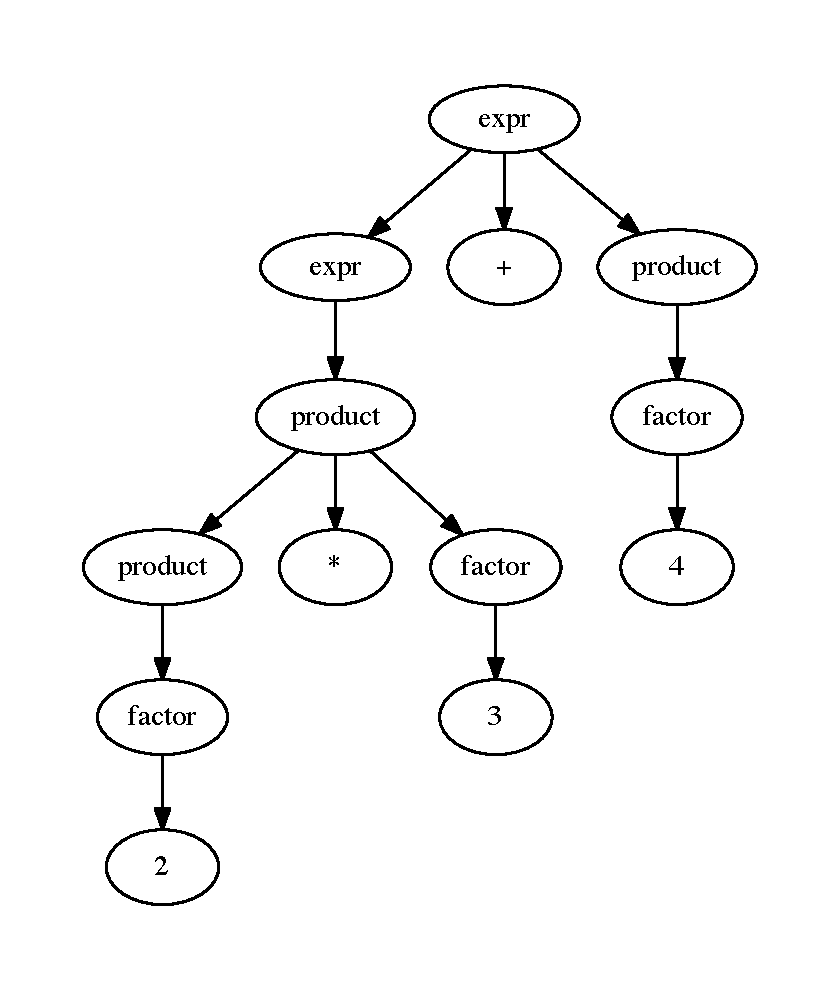
\epsfig{file=Abbildungen/parse-tree.eps, scale=0.7}
  \caption{Ein Parse-Baum f�r den String ``\texttt{2*3+4}''.}
  \label{fig:parse-tree.dot}
\end{figure}

Da B�ume der in Abbildung \ref{fig:parse-tree.dot} gezeigten Art sehr schnell zu gro�
werden, vereinfachen wir diese B�ume mit Hilfe der folgenden Regeln:
\begin{enumerate}
\item Ist $n$ ein innerer Knoten, der mit der Variablen $A$ beschriftet ist
      und gibt es unter den Kindern dieses Knotens genau ein Kind, dass mit einem Terminal $o$
      beschriftet ist,  so entfernen wir dieses Kind und beschriften den Knoten $n$ stattdessen mit dem
      Terminal $o$.
\item Hat ein innerer Knoten nur ein Kind, so ersetzen wir diesen Knoten durch sein Kind.
\end{enumerate}
Den Baum, den wir auf diese Weise erhalten, nennen wir den \blue{abstrakten Syntax-Baum}.
Abbildung \ref{fig:abstract-syntax-tree.dot} zeigt den abstrakten Syntax-Baum den wir
erhalten, wenn wir den in Abbildung \ref{fig:parse-tree.dot} gezeigten Parse-Baum nach
diesen Regeln vereinfachen.  Die in diesem Baum gespeicherte Struktur ist genau das, was
wir brauchen um den arithmetischen Ausdruck ``\texttt{2*3+4}'' auszuwerten, denn der Baum zeigt uns,
in welcher Reihenfolge die Operatoren ausgewertet werden m�ssen.

\begin{figure}[!ht]
  \centering
      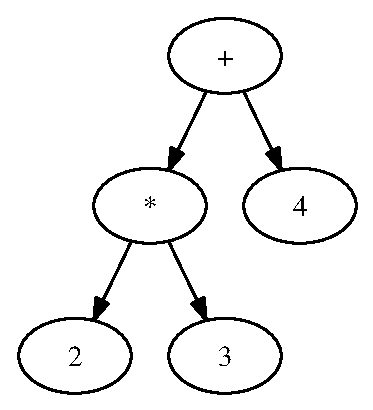
\epsfig{file=Abbildungen/abstract-syntax-tree.eps, scale=0.7}
  \caption{Ein abstrakter Syntax-Baum f�r den String ``\texttt{2*3+4}''.}
  \label{fig:abstract-syntax-tree.dot}
\end{figure}

\subsection{Mehrdeutige Grammatiken}
Die zu Anfang des Abschnitts \ref{kontextfreie} angegebene Grammatik zur Beschreibung arithmetischer
Ausdr�cke erscheint durch ihre Unterscheidung der syntaktischen Kategorien \textsl{arithExpr},
\textsl{product} und \textsl{factor} unn�tig kompliziert.  Wir stellen eine einfachere Grammatik $G$
vor, welche dieselbe Sprache beschreibt:
\\[0.2cm]
\hspace*{1.3cm}
$G = \bigl\langle \{\textsl{expr}\}, \{ \textsc{Number}, \textsc{Variable}, \quoted{+}, \quoted{-}, \quoted{*}, \quoted{/}, \quoted{(}, \quoted{)} \}, R, \textsl{expr} \bigr\rangle$,
\\[0.2cm]
wobei die Regeln $R$ wie folgt gegeben sind:
\begin{eqnarray*}
  \textsl{expr} & \rightarrow & \textsl{expr} \quoted{+} \textsl{expr}  \\
                & \mid        & \textsl{expr} \quoted{-} \textsl{expr}  \\
                & \mid        & \textsl{expr} \quoted{*} \textsl{expr}  \\
                & \mid        & \textsl{expr} \quoted{/} \textsl{expr}  \\
                & \mid        & \quoted{(} \textsl{expr} \quoted{)}     \\
                & \mid        & \textsc{Number}                         \\
                & \mid        & \textsc{Variable}                         
\end{eqnarray*}
Um zu zeigen, dass der String ``\texttt{2*3+4}'' in der von dieser Sprache erzeugten
Grammatik liegt, geben wir die folgende Ableitung an:
\begin{eqnarray*}
\textsl{expr} & \Rightarrow & \textsl{expr} \quoted{+} \textsl{expr}                           \\
              & \Rightarrow & \textsl{expr} \quoted{*} \textsl{expr} \quoted{+} \textsl{expr}  \\
              & \Rightarrow & \texttt{2} \quoted{*} \textsl{expr} \quoted{+} \textsl{expr}     \\
              & \Rightarrow & \texttt{2} \quoted{*} \texttt{3} \quoted{+} \textsl{expr}        \\
              & \Rightarrow & \texttt{2} \quoted{*} \texttt{3} \quoted{+} \texttt{4}           
\end{eqnarray*}
Diese Ableitung entspricht dem abstrakten Syntax-Baum, der in Abbildung
\ref{fig:abstract-syntax-tree.dot}
gezeigt ist.  Es gibt aber noch eine andere Ableitung des Strings ``\texttt{2*3+4}'' mit dieser Grammatik:
\begin{eqnarray*}
\textsl{expr} & \Rightarrow & \textsl{expr} \quoted{*} \textsl{expr}                           \\
              & \Rightarrow & \textsl{expr} \quoted{*} \textsl{expr} \quoted{+} \textsl{expr}  \\
              & \Rightarrow & \texttt{2} \quoted{*} \textsl{expr} \quoted{+} \textsl{expr}     \\
              & \Rightarrow & \texttt{2} \quoted{*} \texttt{3} \quoted{+} \textsl{expr}        \\
              & \Rightarrow & \texttt{2} \quoted{*} \texttt{3} \quoted{+} \texttt{4}           
\end{eqnarray*}
Dieser Ableitung entspricht der abstrakte Syntax-Baum, der in Abbildung
\ref{fig:abstract-syntax-tree-prod.dot} gezeigt ist.
Bei dieser Ableitung wird der String ``\texttt{2*3+4}'' offenbar als Produkt aufgefasst,
was der Konvention widerspricht, dass der Operator ``\texttt{*}'' st�rker bindet als der Operator
``\texttt{+}''.  W�rden wir den String anhand des letzten Syntax-Baums auswerten, w�rden wir
offenbar ein falsches Ergebnis bekommen! 
\begin{figure}[!ht]
  \centering
      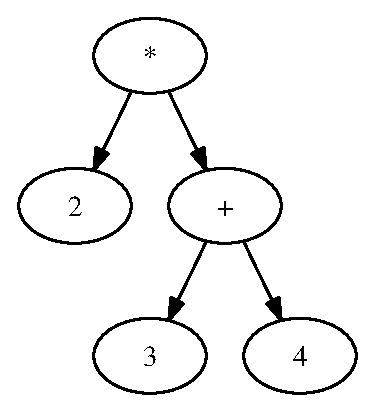
\epsfig{file=Abbildungen/abstract-syntax-tree-prod.eps, scale=0.6}
  \caption{Ein anderer abstrakter Syntax-Baum f�r den String ``\texttt{2*3+4}''.}
  \label{fig:abstract-syntax-tree-prod.dot}
\end{figure}
Die Ursache dieses Problems ist die Tatsache, dass die zuletzt angegebene Grammatik \underline{mehrdeuti}g ist.
Eine solche Grammatik ist zum Parsen ungeeignet.  Leider ist die Frage, ob eine gegebene
Grammatik mehrdeutig ist, im Allgemeinen nicht
\href{http://en.wikipedia.org/wiki/Ambiguous_grammar#Recognizing_ambiguous_grammars}{entscheidbar}:
Es l�sst sich zeigen, dass diese Frage zum
\href{http://en.wikipedia.org/wiki/Post_correspondence_problem}{\blue{Postschen Korrespondenz-Problem}} 
�quivalent ist.  Da das Postsche Korrespondenz-Problem als unl�sbar nachgewiesen wurde, ist auch die
Frage, ob eine Grammatik mehrdeutig ist, unl�sbar.
Ein Beweis dieser Behauptungen findet sich beispielsweise in dem Buch von Hopcroft, Motwani und
Ullman \cite{hopcroft:06}. 


\example
Es sei $\Sigma = \{ \squoted{A}, \squoted{B} \}$.  Die Sprache $L$ enthalte alle die W�rter
aus $\Sigma^*$, bei denen die Buchstaben \squoted{A} and \squoted{B} mit der gleichen
H�ufigkeit auftreten, es gilt also
\\[0.2cm]
\hspace*{1.3cm}
$L = \bigl\{ w \in \Sigma^* \mid \textsl{count}(w, \squoted{A}) = \textsl{count}(w, \squoted{B}) \bigr\}$.
\\[0.2cm]
Dann wird die Sprache $L$ durch die kontextfreie Grammatik $G_1 = \langle \{s\}, \Sigma, R_1, s \rangle$ beschrieben,
deren Regeln wie folgt gegeben sind:
\\[0.2cm]
\hspace*{1.3cm}
$\textsl{s} \;\rightarrow\; \quoted{A} s \quoted{B} s \;\mid\; \quoted{B} s \quoted{A} s \;\mid\; \varepsilon$
\\[0.2cm]
Der Grund ist, dass ein String $w \in L$ entweder mit einem \squoted{A} oder mit einem \squoted{B}
beginnt.  Im ersten Fall muss es zu diesem \squoted{A} ein korrespondierendes \squoted{B} geben, denn
die Anzahl der Auftreten von \squoted{A} und \squoted{B} sind gleich.  Fassen wir den Buchstaben
\squoted{A} wie eine �ffnende Klammer auf und interpretieren den Buchstaben \squoted{B} als die zu
\squoted{A} korrespondierende schlie�ende Klammer, so ist klar, dass der String, der zwischen diesen
beiden Auftreten von \squoted{A} und \squoted{B} liegt, ebenfalls gleich viele Auftreten von
\squoted{A} wie von \squoted{B} hat.  Genauso muss dies dann f�r den Rest des Strings gelten, der nach
dem \squoted{B} folgt.  Diese �berlegung erkl�rt die Regel
\\[0.2cm]
\hspace*{1.3cm}
$\textsl{s} \;\rightarrow\; \quoted{A} s \quoted{B} s$
\\[0.2cm]
Die Regel
\\[0.2cm]
\hspace*{1.3cm}
$\textsl{s} \;\rightarrow\; \quoted{B} s \quoted{A} s$
\\[0.2cm]
l�sst sich in analoger Weise erkl�ren,  wenn wir den Buchstaben \squoted{B} als �ffnende Klammer und
\squoted{A} als schlie�ende Klammer interpretieren. 

Diese Grammatik ist allerdings mehrdeutig: Betrachten wir beispielsweise den String 
``\texttt{abab}'', so stellen wir fest, dass sich dieser prinzipiell auf zwei Arten ableiten l�sst:
\begin{eqnarray*}
  s & \Rightarrow &\quoted{A} s \quoted{B} s                       \\
    & \Rightarrow &\quoted{A} \quoted{B} s                         \\
    & \Rightarrow &\quoted{A} \quoted{B}\quoted{A} s \quoted{B} s \\
    & \Rightarrow &\quoted{A} \quoted{B}\quoted{A} \quoted{B} s   \\
    & \Rightarrow &\quoted{A} \quoted{B}\quoted{A} \quoted{B} 
\end{eqnarray*}
Eine andere Ableitung desselben Strings ergibt sich, wenn wir im zweiten Ableitungs-Schritt nicht das erste
$s$ durch $\varepsilon$ ersetzen sondern stattdessen das zweite $s$ durch $\varepsilon$ ersetzen:
\begin{eqnarray*}
  s & \Rightarrow &\quoted{A} s \quoted{B} s                       \\
    & \Rightarrow &\quoted{A} s \quoted{B}                         \\
    & \Rightarrow &\quoted{A} \quoted{B} s\quoted{A} s \quoted{B} \\
    & \Rightarrow &\quoted{A} \quoted{B}\quoted{A} s \quoted{B}   \\
    & \Rightarrow &\quoted{A} \quoted{B}\quoted{A} \quoted{B}     \\
\end{eqnarray*}
Abbildung \ref{fig:ambiguous-a.dot} zeigt die Parse-B�ume, die sich aus den beiden Ableitungen ergeben.
Wir k�nnen erkennen, dass die Struktur dieser B�ume unterschiedlich ist:  Im ersten Fall geh�rt das erste
``\texttt{A}'' zu dem ersten ``\texttt{B}'', im zweiten Fall geh�rt das erste ``\texttt{A}'' zu dem letzten
``\texttt{B}''.

\begin{figure}[!ht]
      \epsfig{file=Abbildungen/ambiguous-a.eps, scale=0.6}
\quad
      \epsfig{file=Abbildungen/ambiguous-b.eps, scale=0.6}
  \caption{Zwei strukturell verschiedene Parse-B�ume f�r den String ``\texttt{ABAB}''.}
  \label{fig:ambiguous-a.dot}
\end{figure}

Wir definieren nun eine  kontextfreie Grammatik $G_2 = \langle \{s, u, v, x, y\}, \Sigma, R_2, s \rangle$,
deren Regeln wie folgt gegeben sind:
\hspace*{1.3cm}
\begin{eqnarray*}
\textsl{s} & \rightarrow & \textsl{u} \textsl{s} \;\mid\; \textsl{v} \textsl{s} \;\mid\; \varepsilon \\[0.2cm]
\textsl{u} & \rightarrow &\quoted{A} \textsl{x} \quoted{B}                \\[0.2cm]
\textsl{v} & \rightarrow & \quoted{B} \textsl{y} \quoted{A}                \\[0.2cm]
\textsl{x} & \rightarrow & \textsl{u} \textsl{x} \;\mid\; \varepsilon \\[0.2cm]
\textsl{y} & \rightarrow & \textsl{v} \textsl{y} \;\mid\; \varepsilon          
\end{eqnarray*}
Um die Sprachen, die von den einzelnen Variablen erzeugt werden, klarer beschreiben zu
k�nnen, definieren wir f�r zwei Strings $\sigma$ und $\omega$ die Relation $\sigma \preceq \omega$ (lese: $\sigma$ ist ein
Pr�fix von $\omega$) wie folgt:
\\[0.2cm]
\hspace*{1.3cm}
$\sigma \preceq \omega \quad \stackrel{\rm{def}}{\Longleftrightarrow} \exists \tau \in \Sigma^*: \sigma \tau = \omega$
\\[0.2cm]
Sodann bemerken wir, dass von den syntaktischen Variablen $x$ und $y$ die folgenden
Sprachen erzeugt werden:
\\[0.2cm]
\hspace*{1.3cm} 
$L(x) = \bigl\{ \omega \in \Sigma^* \mid \omega \in L \;\wedge\; \forall \sigma \preceq \omega : 
                  \textsl{count}(\sigma,\squoted{B}) \leq \textsl{count}(\sigma,\squoted{A}) \bigr\}$
\quad und \\[0.2cm]
\hspace*{1.3cm}
$L(y) = \bigl\{ \omega \in \Sigma^* \mid \omega \in L \;\wedge\; \forall \sigma \preceq \omega : 
                  \textsl{count}(\sigma, \squoted{A}) \leq \textsl{count}(\sigma, \squoted{B}) \bigr\}$.
\\[0.2cm]
Ist $w \in L(x)$, so gibt es zu jedem Auftreten des Buchstabens ``\texttt{B}'' in dem String $w$ ein
dazu korrespondierendes Auftreten des Buchstabens ``\texttt{A}'', das dem Auftreten des Buchstabens
``\texttt{B}'' vorangeht.  W�rden wir den Buchstaben
``\texttt{A}'' durch eine �ffnende Klammer und den Buchstaben ``\texttt{B}'' durch eine schlie�ende
Klammer ersetzen, so wird also niemals eine Klammer geschlossen, die nicht vorher ge�ffnet wurde.
Damit ist klar, dass in einem String der Form
\\[0.2cm]
\hspace*{1.3cm}
``\texttt{A}'' $w$ ``\texttt{B}'' \quad mit $w \in L(x)$ 
\\[0.2cm]
das zu dem ersten ``\texttt{A}'' korrespondierende ``\texttt{B}'' nur das letzte ``\texttt{B}'' sein kann.
Analog k�nnen wir sehen, dass in einem String der Form
\\[0.2cm]
\hspace*{1.3cm}
``\texttt{B}'' $w$ ``\texttt{A}'' \quad mit $w \in L(Y)$ 
\\[0.2cm]
das zu dem ersten ``\texttt{B}'' korrespondierende ``\texttt{A}'' nur das letzte ``\texttt{A}'' sein kann.

Ein String der Sprache $L$ f�ngt nun entweder mit ``\texttt{A}'' oder mit ``\texttt{B}''
an.  Im ersten Fall interpretieren wir das ``\texttt{A}'' als �ffnende Klammer und 
das ``\texttt{B}'' als schlie�ende Klammer und suchen nun das ``\texttt{B}'', das dem
``\texttt{A}'' am Anfang des Strings zugeordnet ist.  Der String, der mit dem
``\texttt{A}'' anf�ngt und dem ``\texttt{B}'' endet, liegt in der Sprache $L(u)$.
Auf dieses ``\texttt{B}'' kann dann noch ein weiterer Teilstring folgen, der
gleich viele ``\texttt{A}''s und ``\texttt{B}''s enth�lt.  Ein solcher Teilstring liegt
offensichtlich ebenfalls in der Sprache $L$ und kann daher von $s$ mittels der Regel
\\[0.2cm]
\hspace*{1.3cm}
$\textsl{s} \rightarrow \textsl{u}\textsl{s}$
\\[0.2cm]
erzeugt werden.
Im zweiten Fall f�ngt der String mit einem ``\texttt{B}'' an.  Dieser Fall ist
analog zum ersten Fall.    \qed
\vspace*{0.3cm}

In dem obigen Beispiel hatten wir Gl�ck und konnten eine Grammatik finden, mit der sich
die Sprache eindeutig parsen l�sst.  Es  gibt allerdings auch kontextfreie Sprachen, die 
\href{http://en.wikipedia.org/wiki/Ambiguous_grammar#Inherently_ambiguous_languages}{inh�rent mehrdeutig}
sind: Es l�sst sich beispielsweise zeigen, dass f�r das Alphabet 
$\Sigma =  \{ \squoted{A}, \squoted{B}, \squoted{C}, \squoted{D} \}$
die Sprache
\\[0.2cm]
\hspace*{1.3cm}
$L =  \bigl\{ \mathtt{A}^m \mathtt{B}^m \mathtt{C}^n \mathtt{D}^n \mid m, n \in \mathbb{N} \bigr\}
 \cup \bigl\{ \mathtt{A}^m \mathtt{B}^n \mathtt{C}^n \mathtt{D}^m \mid m, n \in \mathbb{N} \bigr\}
$
\\[0.2cm]
kontextfrei ist, aber jede Grammatik $G$ mit der Eigenschaft $L = L(G)$ ist
notwendigerweise mehrdeutig.  Das Problem ist, dass f�r gewisse gro�e Zahlen $n\in \mathbb{N}$ ein
String der Form 
\\[0.2cm]
\hspace*{1.3cm}
$\mathtt{A}^n \mathtt{B}^n \mathtt{C}^n \mathtt{D}^n$
\\[0.2cm]
immer zwei strukturell verschiedene Parse-B�ume besitzen muss.  Ein Beweis dieser Behaupung
findet sich in der ersten Auflage des Buchs von  Hopcroft und Ullman auf Seite 100 \cite{hopcroft:79}.   

\section{Top-Down-Parser}
In diesem Abschnitt stellen wir ein Verfahren vor, mit dem sich eine ganze Reihe von
Grammatiken bequem parsen lassen.  Die Grundidee ist einfach:  Um einen String $w$ mit
Hilfe einer Grammatik-Regel der Form
\\[0.2cm]
\hspace*{1.3cm}
$\textsl{a} \rightarrow \textsl{X}_1 \textsl{X}_2 \cdots \textsl{X}_n$
\\[0.2cm]
zu parsen, versuchen wir, zun�chst ein $X_1$ zu parsen.  Dabei zerlegen wir den String $w$ in die
Form
$w = w_1 r_1$ so, dass $w_1 \in L(X_1)$ gilt.  Dann versuchen wir, in dem Rest-String
$r_1$ ein $X_2$ zu parsen und zerlegen dabei $r_1$ so, dass $r_1 = w_2 r_2$ mit 
$w_2 \in L(X_2)$ gilt.  Setzen wir diesen Prozess fort, so haben wir zum Schluss den String $w$ in
\\[0.2cm]
\hspace*{1.3cm}
$w = w_1 w_2 \cdots w_n$ \quad mit $w_i \in L(X_i)$ f�r alle $i=1,\cdots,n$
\\[0.2cm]
aufgespaltet.  Leider funktioniert dieses Verfahren dann nicht, wenn die Grammatik
\blue{links-rekursiv} ist, das hei�t, dass eine Regel die Form
\\[0.2cm]
\hspace*{1.3cm}
$\textsl{a} \rightarrow \textsl{a} \beta$
\\[0.2cm]
hat, denn dann w�rden wir um ein $\textsl{a}$ zu parsen sofort wieder rekursiv versuchen, 
ein $a$ zu parsen und w�ren damit in einer Endlos-Schleife.  Es gibt mehrere M�glichkeiten, um mit
diesem Problem umzugehen:
\begin{enumerate}
\item Wir k�nnen die Grammatik so umschreiben, dass sie danach nicht mehr links-rekursiv
      ist.
\item Eine einfachere Methode besteht darin, denn Begriff der kontextfreien Grammatik
      zu erweitern.  Wir werden den Begriff der \blue{erweiterten Backus-Naur-Form}-Grammatik
      (abgek�rzt \textsc{Ebnf}-Grammatik) einf�hren.  Hierbei handelt es sich um eine Verallgemeinerung des
      Begriffs der kontextfreien Grammatik.  Theoretisch ist die Ausdrucksst�rke der
      \textsc{Ebnf}-Grammatiken dieselbe wie die Ausdrucksst�rke der kontextfreien Grammatiken.
      In der Praxis zeigt sich aber, dass die Konstruktion von Top-Down-Parsern f�r
      \textsc{Ebnf}-Grammatiken einfacher ist, weil dort die Links-Rekursion durch eine Iteration ersetzt
      werden kann.
\end{enumerate}
Im Rahmen dieses Kapitels werden wir die beiden oben genannten Verfahren anhand der Grammatik f�r
arithmetische Ausdr�cke ausf�hrlich diskutieren.  

\subsection{Umschreiben der Grammatik$^*$ \label{links-rekursion}}
In der folgenden Grammatik ist $a$ eine syntaktische Variable und die griechischen Buchstaben $\beta$ und
$\gamma$ stehen f�r irgendwelche Strings, die aus syntaktischen Variablen und Tokens bestehen.
Wird die syntaktische Variable $a$ durch die beiden Regeln
\\[0.2cm]
\hspace*{1.3cm}
$
\begin{array}[t]{lcl}
a & \rightarrow & a \beta \\
  & \mid        & \gamma
\end{array}
$
\\[0.2cm]
definiert, so hat eine Ableitung von $a$, bei der zun�chst immer die syntaktische Variable $a$ ersetzt
wird, die Form 
\\[0.2cm]
\hspace*{1.3cm}
$a \Rightarrow a \beta \Rightarrow a \beta \beta \Rightarrow a \beta \beta \beta
 \Rightarrow \cdots \Rightarrow a \beta^n \Rightarrow \gamma \beta^n$.
\\[0.2cm]
Damit sehen wir, dass die durch die syntaktische Variable $a$ beschriebene Sprache $L(a)$ aus allen den
Strings besteht, die sich aus dem Ausdruck $\gamma \beta^n$ ableiten lassen:
\\[0.2cm]
\hspace*{1.3cm}
$L(a) = \bigl\{ w \in \Sigma^* \mid \exists n \in \mathbb{N}: \gamma \beta^n \Rightarrow^* w \bigr\}$.
\\[0.2cm]
Diese Sprache kann offenbar auch durch die folgenden Regeln f�r $a$ beschrieben werden:
\\[0.2cm]
\hspace*{1.3cm}
$
\begin{array}[t]{lcl}
a & \rightarrow & \gamma b \\[0.2cm]
b & \rightarrow & \beta b  \\
  & \mid        & \varepsilon 
\end{array}
$
\\[0.2cm]
Hier haben wir die Hilfs-Variable $b$ eingef�hrt.  Die Ableitungen, die von dem Nicht-Terminal $b$
ausgehen, haben die Form
\\[0.2cm]
\hspace*{1.3cm} $b \Rightarrow \beta b \Rightarrow \beta \beta b \Rightarrow \cdots \Rightarrow
\beta^n b \Rightarrow \beta^n$.
\\[0.2cm]
Folglich beschreibt das Nicht-Terminal $b$ die Sprache
\\[0.2cm]
\hspace*{1.3cm} $L(b) = \bigl\{ w \in \Sigma \mid \exists n \in \mathbb{N}: \beta^n \Rightarrow w
\bigr\}$.
\\[0.2cm]
Damit ist klar, dass auch mit der oben angegeben Grammatik
\\[0.2cm]
\hspace*{1.3cm} $L(a) = \bigl\{ w \in \Sigma^* \mid \exists n \in \mathbb{N}: \gamma \beta^n
\Rightarrow^* w \bigr\}$
\\[0.2cm]
gilt.  Um die Links-Rekursion aus der in Abbildung \ref{fig:Expr} auf Seite \pageref{fig:Expr}
gezeigten Grammatik zu entfernen, m�ssen wir das obige Beispiel verallgemeinern.  Wir betrachten
jetzt den allgemeinen Fall und nehmen an, dass ein Nicht-Terminal $a$ durch Regeln der Form
\\[0.2cm]
\hspace*{1.3cm} $
\begin{array}[t]{lcl}
a & \rightarrow & a \beta_1 \\
  & \mid        & a \beta_2 \\
  & \vdots      & \vdots    \\
  & \mid        & a \beta_k \\[0.2cm]
  & \mid        & \gamma_1  \\
  & \vdots      & \vdots    \\
  & \mid        & \gamma_l
\end{array}
$
\\[0.2cm]
beschrieben wird.  Wir k�nnen diesen Fall durch Einf�hrung zweier Hilfs-Variablen $b$ und $c$ auf
den ersten Fall zur�ckf�hren:
\\[0.2cm]
\hspace*{1.3cm}
$
\begin{array}[t]{lcl}
a & \rightarrow & a b \mid c                         \\[0.2cm]
b & \rightarrow & \beta_1 \mid \cdots \mid \beta_k   \\[0.2cm]
c & \rightarrow & \gamma_1 \mid \cdots \mid \gamma_l
\end{array}
$
\\[0.2cm]
Dann k�nnen wir die Grammatik umschreiben, indem wir eine neue Hilfs-Variable, nennen wir sie $l$
f�r Liste, einf�hren und erhalten
\\[0.2cm]
\hspace*{1.3cm}
$
\begin{array}[t]{lcl}
a & \rightarrow & c\;l                   \\[0.2cm]
l & \rightarrow & b\;l \mid \varepsilon.  
\end{array}
$
\\[0.2cm]
Die Hilfs-Variablen $b$ und $c$ k�nnen nun wieder eliminiert werden und dann bekommen wir die folgende
Grammatik: 
\\[0.2cm]
\hspace*{1.3cm}
$
\begin{array}[t]{lcl}
a & \rightarrow & \gamma_1\;l \;\mid\; \gamma_2\;l \;\mid\; \cdots \;\mid\; \gamma_l\;l  \\[0.2cm]
l & \rightarrow & \beta_1 \;l \;\mid\; \beta_2 \;l \;\mid\; \cdots \;\mid\; \beta_k \;l \;\mid\; \varepsilon
\end{array}
$
\begin{figure}[htbp]
  \begin{center}    
  \framebox{
  \framebox{
  \begin{minipage}[t]{8cm}
  \begin{eqnarray*}
  \textsl{expr}    & \rightarrow & \;\textsl{expr} \quoted{+} \textsl{product}  \\
                   & \mid        & \;\textsl{expr} \quoted{-} \textsl{product}  \\
                   & \mid        & \;\textsl{product}                           \\[0.2cm]
  \textsl{product} & \rightarrow & \;\textsl{product} \quoted{*} \textsl{factor}\\
                   & \mid        & \;\textsl{product} \quoted{/} \textsl{factor}\\
                   & \mid        & \;\textsl{factor}                            \\[0.2cm]
  \textsl{factor}  & \rightarrow &   \quoted{(} \textsl{expr} \quoted{)}        \\
                   & \mid        & \;\textsc{Number} 
  \end{eqnarray*}
  \vspace*{-0.5cm}
  \end{minipage}}}
  \end{center}
  \caption{Links-rekursive Grammatik f�r arithmetische Ausdr�cke.}
  \label{fig:Expr}
\end{figure}
\vspace*{0.3cm}

\noindent
Wenden wir dieses Verfahren auf die in Abbildung \ref{fig:Expr} gezeigte Grammatik f�r arithmetische
Ausdr�cke an, so erhalten wir die in Abbildung \ref{fig:Expr2} gezeigte Grammatik.

\begin{figure}[htbp]
  \begin{center}    
  \framebox{
  \framebox{
  \begin{minipage}[t]{9cm}
  \begin{eqnarray*}
  \textsl{expr}        & \rightarrow & \;\textsl{product}\;\;\textsl{exprRest}            \\[0.2cm]
  \textsl{exprRest}    & \rightarrow & \quoted{+} \textsl{product}\;\;\textsl{exprRest}   \\
                       & \mid        & \quoted{-} \textsl{product}\;\;\textsl{exprRest}   \\
                       & \mid        & \;\varepsilon                                      \\[0.2cm]
  \textsl{product}     & \rightarrow & \;\textsl{factor}\;\;\textsl{productRest}          \\[0.2cm]
  \textsl{productRest} & \rightarrow & \quoted{*} \textsl{factor}\;\;\textsl{productRest} \\
                       & \mid        & \quoted{/} \textsl{factor}\;\;\textsl{productRest} \\
                       & \mid        & \;\varepsilon                                      \\[0.2cm]
  \textsl{factor}      & \rightarrow & \quoted{(} \textsl{expr} \quoted{)}                \\
                       & \mid        & \;\textsc{Number} 
  \end{eqnarray*}
  \vspace*{-0.5cm}
  \end{minipage}}}
  \end{center}
  \caption{Grammatik f�r arithmetische Ausdr�cke ohne Links-Rekursion.}
  \label{fig:Expr2}
\end{figure}
\pagebreak

\noindent
Die Variablen \textsl{exprRest} und \textsl{productRest} k�nnen wie folgt interpretiert werden:
\begin{enumerate}
\item \textsl{exprRest} beschreibt eine Liste der Form
      \\[0.2cm]
      \hspace*{1.3cm}
      $\textsl{op} \;\textsl{product} \;\cdots \;\textsl{op}\; \textsl{product}$,
      \\[0.2cm]
      wobei $\textsl{op} \in \{ \quoted{+}, \quoted{-} \}$ gilt.
\item \textsl{productRest} beschreibt eine Liste der Form
      \\[0.2cm]
      \hspace*{1.3cm}
      $\textsl{op} \;\textsl{factor} \;\cdots \;\textsl{op} \;\textsl{factor}$,
      \\[0.2cm]
      wobei $\textsl{op} \in \{ \quoted{*}, \quoted{/} \}$ gilt. 
\end{enumerate}


\exercise
\begin{enumerate}
\item[(a)] Die folgende Grammatik beschreibt regul�re Ausdr�cke:
      \begin{center}    
          \framebox{
            \begin{minipage}[t]{9cm}
              \begin{eqnarray*}
                \textsl{regExp} & \rightarrow & \;\textsl{regExp} \quoted{+} \textsl{regExp}    \\
                                & \mid        & \;\textsl{regExp} \;\;\textsl{regExp}           \\
                                & \mid        & \;\textsl{regExp}\quoted{*}                     \\
                                & \mid        & \quoted{(} \textsl{regExp} \quoted{)}           \\
                                & \mid        & \;\textsc{Letter}                               
              \end{eqnarray*}
              \vspace*{-0.5cm}
            \end{minipage}}
      \end{center}
      Diese Grammatik verwendet nur die  syntaktische Variable $\{ \textsl{regExp} \}$ und die folgenden 
      Terminale
      \\[0.2cm]
      \hspace*{1.3cm}
      \squoted{+}, \squoted{*}, \squoted{(}, \squoted{)}, \textsc{Letter}.
      \\[0.2cm]
      Da die Grammatik mehrdeutig ist, ist diese Grammatik zum Parsen ungeeignet.
      Transformieren Sie diese Grammatik in eine eindeutige Grammatik, bei welcher der
      Postfix-Operator ``\texttt{*}'' st�rker bindet als die Konkatenation zweier regul�rer
      Ausdr�cke, w�hrend der Operator ``\texttt{+}'' schw�cher bindet als die Konkatenation. 
      Orientieren Sie sich dabei an der Grammatik f�r arithmetische Ausdr�cke und f�hren
      Sie geeignete neue syntaktische Variablen ein.
\item[(b)] Entfernen Sie die Links-Rekursion aus der in Teil (a) dieser Aufgabe erstellten
      Grammatik. \eox
\end{enumerate}



\subsection{Implementing a Top Down Parser in \textsl{Python}}


\begin{figure}[!ht]
\centering
\begin{minted}[ frame         = lines, 
                framesep      = 0.3cm, 
                bgcolor       = sepia,
                numbers       = left,
                numbersep     = -0.2cm,
                xleftmargin   = 0.0cm,
                xrightmargin  = 0.0cm
              ]{python3}
    import re
    
    def tokenize(s):
        lexSpec = r'''([ \t]+)        |  # blanks and tabs
                      ([1-9][0-9]*|0) |  # number
                      ([()])          |  # parentheses 
                      ([-+*/])        |  # arithmetical operators
                      (.)                # unrecognized character
                   '''
        tokenList = re.findall(lexSpec, s, re.VERBOSE)
        result    = []
        for ws, number, parenthesis, operator, error in tokenList:
            if ws:        # skip blanks and tabs
                pass
            if number:
                result += [ number ]
            if parenthesis:
                result += [ parenthesis ]
            if operator:
                result += [ operator ]
            if error:
                result += [ f'ERROR({error})']
        return result
\end{minted}
\vspace*{-0.3cm}
\caption{A scanner for arithmetic expressions.}
\label{fig:Top-Down-Parser:scanner.ipynb}
\end{figure}


\begin{figure}[!ht]
\centering
\begin{minted}[ frame         = lines, 
                framesep      = 0.3cm, 
                bgcolor       = sepia,
                numbers       = left,
                numbersep     = -0.2cm,
                xleftmargin   = 0.0cm,
                xrightmargin  = 0.0cm
              ]{python3}
    def parse(s):
         TL           = tokenize(s)
         result, Rest = parseExpr(TL)
         assert Rest == [], f'Parse Error: could not parse {TL}'
         return result
    
    def parseExpr(TL):
        product, Rest = parseProduct(TL)
        return parseExprRest(product, Rest)
    
    def parseExprRest(sum, TL):
        if TL == []:
            return sum, []
        elif TL[0] == '+':
            product, Rest = parseProduct(TL[1:])
            return parseExprRest(sum + product, Rest)
        elif TL[0] == '-':
            product, Rest = parseProduct(TL[1:])
            return parseExprRest(sum - product, Rest)
        else:
            return sum, TL
    
    def parseProduct(TL):
        factor, Rest = parseFactor(TL)
        return parseProductRest(factor, Rest)
    
    def parseProductRest(product, TL):
        if TL == []:
            return product, []
        elif TL[0] == '*': 
            factor, Rest = parseFactor(TL[1:])
            return parseProductRest(product * factor, Rest)
        elif TL[0] == '/':
            factor, Rest = parseFactor(TL[1:])
            return parseProductRest(product / factor, Rest)
        else:
            return product, TL
    
    def parseFactor(TL):
        if TL[0] == '(': 
            expr, Rest = parseExpr(TL[1:])
            assert Rest[0] == ')', 'Parse Error: expected ")"'
            return expr, Rest[1:]
        else: 
            return int(TL[0]), TL[1:]
\end{minted}
\vspace*{-0.3cm}
\caption{A top down parser for arithmetic expressions.}
\label{fig:Top-Down-Parser.ipynb}
\end{figure}


\noindent
Now we are ready to implement a parser for recognizing arithmetic expressions.
Figure \ref{fig:rd-parser.stlx} on page
\pageref{fig:rd-parser.stlx} shows an implementation of a recursive decent parser in
\textsc{SetlX}. 
\begin{enumerate}
\item The main function is \texttt{myParse}\footnote{
            We had to name the function \texttt{myParse} instead of \texttt{parse} as 
            \textsc{SetlX} already implements a function with the name \texttt{parse}.
            This function parses strings as \textsc{SetlX} expressions.  The function
            \texttt{parse} returns a term representing the abstract syntax tree
            corresponding to the parsed expression.
      }.  This function takes a string $s$
      representing an arithmetic expression.  This string is tokenized using the 
      function \texttt{tokenizeString}.  The function \texttt{tokenizeString} turns a
      string into a list of tokens.  For example, the expression
      \\[0.2cm]
      \hspace*{1.3cm}
      \verb|tokenizeString("(1 + 2) * 3");|
      \\[0.2cm]
      returns the result
      \\[0.2cm]
      \hspace*{1.3cm}
      \verb|["(", 1, "+", 2, ")", "*", 3]|.
      \\[0.2cm]
      This list of tokens is then parsed by the function \texttt{parseExpr}.
      That function returns a pair: 
      \begin{enumerate}
      \item The first  component is the value of the arithmetic expression.
      \item The second component is the list of those tokens that have not been consumed
            when parsing the expression.  Of course, on a successful parse this list
            should be empty.
      \end{enumerate}
\item The function \texttt{parseExpr} implements the grammar rule
      \\[0.2cm]
      \hspace*{1.3cm}
      $\textsl{expr} \;\rightarrow\;\textsl{product}\;\;\textsl{exprRest}$. 
      \\[0.2cm]
      It takes a token list \texttt{tl} as input.  It will return a pair of the form
      \\[0.2cm]
      \hspace*{1.3cm}
      \texttt{[$v$, rl]},
      \\[0.2cm]
      where $v$ is the value of the arithmetic expression that has been parsed, while
      \texttt{rl} is the list of the remaining tokens.  For example, the expression
      \\[0.2cm]
      \hspace*{1.3cm}
      \verb|parseExpr(["(", 1, "+", 2, ")", "*", 3, ")", "*", 2])|
      \\[0.2cm]
      returns the result
      \\[0.2cm]
      \hspace*{1.3cm}
      \verb|[9, [")", "*", 2]]|.
      \\[0.2cm]
      Here, the part \verb|["(", 1, "+", 2, ")", "*", 3]| has been parsed and evaluated as
      the number $9$ and \verb|[")", "*", 2]| is the list of tokens that have not yet been
      processed.

      In order to parse an arithmetic expression, the function first parses a
      \textsl{product} and then it tries to parse the remaining tokens as an
      \textsl{exprRest}.   The function \texttt{parseExprRest} that is used to parse an
      \textsl{exprRest} needs two arguments:
      \begin{enumerate}
      \item The first argument is the value of the product that has been parsed 
            by the function \texttt{parseProduct}.
      \item The second argument is the list of tokens that can be used.
      \end{enumerate}
      To understand the mechanics of \texttt{parseExpr}, consider the evaluation of
      \\[0.2cm]
      \hspace*{1.3cm}
      \verb|[1, "*", 2, "+", 3]|.
      \\[0.2cm]
      Here, the function \texttt{parseProduct} will return the result
      \\[0.2cm]
      \hspace*{1.3cm}
      \verb|[2, ["+", 3]]|,
      \\[0.2cm]
      where $2$ is the result of parsing and evaluating the token list \verb|[1, "*", 2]|, while
      \verb|["+", 3]| is the part of the input token list that is not used by
      \texttt{parseProduct}.  Next, the list \verb|["+", 3]| needs to be parsed as 
      the rest of an expression and then $3$ needs to be added to $2$.      
\item The function \texttt{parseExprRest} takes a number and a list of tokens.
      It implements the following grammar rules:
      \hspace*{1.3cm}
      \begin{eqnarray*}
        \textsl{exprRest} & \rightarrow & \quoted{+} \textsl{product}\;\;\textsl{exprRest} \\
                          & \mid        & \quoted{-} \textsl{product}\;\;\textsl{exprRest} \\
                          & \mid        & \;\varepsilon                                    
      \end{eqnarray*}
      Therefore, it checks whether the first token is either \squoted{+} or \squoted{-}.
      If the token is \squoted{+}, it parses a \textsl{product}, adds the result of this 
      product to the \texttt{sum} of values parsed already and proceeds to parse the rest
      of the tokens.  

      The case that the first token is \squoted{-} is similar to the previous case.
      If the next token is neither \squoted{+} nor \squoted{-}, then it could be either the
      token \squoted{)} or else it might be the case that the list of tokens is already
      exhausted.  In either case, the rule
      \\[0.2cm]
      \hspace*{1.3cm}
      $\textsl{exprRest} \;\rightarrow\; \varepsilon$
      \\[0.2cm]
      is used.  Therefore, in that case we have not consumed any tokens and hence
      the input arguments are already the result.
\item The function \texttt{parseProduct} implements the rule
      \\[0.2cm]
      \hspace*{1.3cm}
      $\textsl{product} \;\rightarrow\; \textsl{factor} \;\; \textsl{exprRest}$.
      \\[0.2cm]
      The implementation is similar to the implementation of \textsl{parseExpr}.
\item The function \texttt{parseProductRest} implements the rules
      \begin{eqnarray*}
      \textsl{productRest} & \rightarrow & \quoted{*} \textsl{factor}\;\;\textsl{productRest} \\
                       & \mid        & \quoted{/} \textsl{factor}\;\;\textsl{productRest}     \\
                       & \mid        & \;\varepsilon                                      
      \end{eqnarray*}
      The implementation is similar to the implementation of \textsl{parseExprRest}.
\item The function \texttt{parseFactor} implements the rules
      \begin{eqnarray*}
      \textsl{factor} & \rightarrow & \quoted{(} \textsl{expr} \quoted{)} \\
                      & \mid        & \;\textsc{Number} 
      \end{eqnarray*}
      Therefore, we first check whether the next token is \squoted{(} because in that case,
      we have to use the first grammar rule, otherwise we use the second.
\item The last function \texttt{tokenizeString} transforms a string into a list of tokens.
      To this end it uses the \texttt{scan} mechanism that is already built into
      \textsc{SetlX}.  For example, in line 43 it is checked whether the next part of the
      input string is matched by the regular expression \verb"0|[1-9][0-9]*".  If this is
      the case, the matching part is choped off the string and converted into a number
      which is then added to the list of tokens seen so far.

      In line 44 we recognize the operator symbols and the parenthesis.  Note that we had
      to put the operator \squoted{-} first here since otherwise it would have been
      mistaken as a range operator.

      Line 45 is needed to skip white space.
\end{enumerate}
The parser shown in Figure \ref{fig:rd-parser.stlx} does not contain any error handling. 
Appropriate error handling will be discussed once we have covered the theory of top-down parsing.


%%% Local Variables: 
%%% mode: latex
%%% TeX-master: "formal-languages.tex"
%%% End: 

\chapter[ANTLR]{ANTLR --- \emph{Another Tool for Language Recognition}}
Es gibt eine Reihe von Werkzeugen, die in der Lage sind, einen Top-Down-Parser automatisch
zu erzeugen.  Das Werkzeug, das in meinen Augen am besten ausgereift ist, ist
\textsc{Antlr} \cite{parr:2012,parr:2013}.  Der Name steht f\"ur 
\emph{\underline{an}other \underline{t}ool for \underline{l}anguage \underline{r}ecognition}\footnote{
Der Name \textsc{Antlr} kann au{\ss}erdem auch als Abk\"urzung f\"ur \underline{ant}i \underline{LR} verstanden
werden. Hier steht ``LR'' f\"ur \emph{LR-Parser}.  Dies ist eine Klasse von Parsern, die nicht \emph{top-down} 
sondern stattdessen \emph{bottom-up} arbeiten.  Wir werden diese Klasse von Parsern sp\"ater noch ausf\"uhrlich 
diskutieren.
}.
Sie finden dieses Werkzeug im Internet unter der folgenden Adresse 
\\[0.2cm]
\hspace*{1.3cm}
\href{http://www.antlr.org}{\texttt{http://www.antlr.org}}.
\\[0.2cm]
In dieser Vorlesung werden wir die Version 4.5.1 verwenden.  Das Werkzeug \textsc{Antlr} ist in der
Lage, Parser in den Sprachen \textsl{Java}, \texttt{C\#} und \textsl{Python} zu erzeugen.

Zun\"achst f\"uhren wir \textsc{Antlr} anhand verschiedener Beispiele ein, durch die wir die 
wichtigsten Eigenschaften des Werkzeugs demonstrieren k\"onnen.  In sp\"ateren Kapiteln werden wir
die Theorie von Top-Down-Parsern untersuchen.
\textsc{Antlr} unterst\"utzt die Verwendung von \textsc{Ebnf}-Grammatiken.  


\section{Ein Parser f\"ur arithmetische Ausdr\"ucke}
Wir beginnen mit einem Parser f\"ur arithmetische Ausdr\"ucke, die entsprechend der in
Abbildung \ref{fig:Expr} auf Seite \pageref{fig:Expr} gezeigten Grammatik aufgebaut sind.
Diese Grammatik l\"asst sich nun mit Hilfe von \textsc{Antlr} wie in Abbildung
\ref{fig:Expr.g4} gezeigt implementieren.  Wir diskutieren diese Umsetzung Zeile f\"ur Zeile.

\begin{figure}[!ht]
\centering
\begin{Verbatim}[ frame         = lines, 
                  framesep      = 0.3cm, 
                  labelposition = bottomline,
                  numbers       = left,
                  numbersep     = -0.2cm,
                  xleftmargin   = 0.8cm,
                  xrightmargin  = 0.8cm,
                ]
    grammar Expr;
    
    start   : expr
            ;
    
    expr    : expr ('+'|'-') product 
            | product        
            ;
    
    product : product ('*'|'/') factor 
            | factor
            ;
    
    factor  : '(' expr ')'
            | NUMBER
            ;
    
    NUMBER  : '0'|[1-9][0-9]*;
    WS      : [ \v\t\n\r] -> skip;
\end{Verbatim}
\vspace*{-0.3cm}
\caption{\textsc{Antlr}-Spezifikation eines Parsers f\"ur arithmetische Ausdr\"ucke.}
\label{fig:Expr.g4}
\end{figure}


\begin{enumerate}
\item In Zeile 1 spezifizieren wir mit dem Schl\"usselwort \texttt{grammar} den Namen der Grammatik.
      In unserem Fall hat die Grammatik also den Namen \texttt{Expr}.  Der Name  der Datei, in der
      die Grammatik abgespeichert ist, wird aus dem Namen der Grammatik durch Anh\"angen der Endung ``\texttt{.g4}''
      gebildet, daher muss die gezeigte Grammatik in einer Datei mit dem Namen ``\texttt{Expr.g4}''
      abgespeichert werden.      
\item Zeile 3 enth\"alt die Grammatik-Regel f\"ur die syntaktische Variable
      \textsl{start}.  Die dort gezeigte Grammatik-Regel entspricht mathematisch der Regel
      \\[0.2cm]
      \hspace*{1.3cm}
      $\textsl{start} \rightarrow \textsl{expr}$.
      \\[0.2cm]
      Beachten Sie, dass linke und rechte Seite einer Grammatik-Regel durch einen Doppelpunkt
      getrennt werden.
      Jede Grammatik-Regel wird durch ein Semikolon ``\texttt{;}'' beendet.
\item Zeile 6 enth\"alt die Grammatik-Regel f\"ur die syntaktische Variable
      \textsl{expr}.  Zu beachten ist hier, dass die Terminale ``\texttt{+}'' und
      ``\texttt{-}'' bei \textsc{Antlr} in einfache Anf\"uhrungszeichen gesetzt werden
      m\"ussen.  Zus\"atzlich sehen wir, dass die
      verschiedenen Grammatikregeln, welche dieselbe syntaktische
      Variable definieren, durch das Zeichen ``\texttt{|}'' von einander getrennt werden.
\item Entsprechend enthalten die Zeilen 10 und 14 die Grammatik-Regeln f\"ur die syntaktischen
      Variablen \textsl{product} und \textsl{factor}.  

\item Bei \textsc{Antlr} werden die grammatikalische Struktur und die lexikalische
      Struktur der Eingabe in derselben Datei definiert.  Um syntaktische Variablen und
      Terminale von einander unterscheiden zu k\"onnen, wird vereinbart, dass Terminale mit
      einem Gro{\ss}buchstaben beginnen,\footnote
      {Es ist Konvention, aber nicht vorgeschrieben, dass die 
      Namen von Terminalen nur aus Gro{\ss}buchstaben bestehen.}
      w\"ahrend syntaktische Variablen immer mit einem kleinen
      Buchstaben beginnen.  
      Daher wissen wir, dass der String ``\texttt{NUMBER}'' in Zeile 8
      ein Terminal bezeichnet.
\item In Zeile 18 wird die lexikalische Struktur der mit \texttt{NUMBER} bezeichneten
      Terminale durch einen regul\"aren Ausdruck definiert.  Der regul\"are Ausdruck
      \\[0.2cm]
      \hspace*{1.3cm}
      \texttt{'0'|[1-9][0-9]*;}
      \\[0.2cm]
      steht hier f\"ur eine Folge aus Ziffern.  Diese Folge von Ziffern kann nur dann mit der Ziffer
      ``\texttt{0}'' beginnen, wenn auf die ``\texttt{0}'' keine weitere Ziffer mehr folgt.

      Notice that we have to enclose the first occurrence of ``\texttt{0}'' in single quotes.
      On the other hand, we must not put the digits occurring in the square brackets ``\texttt{[}'' 
      and ``\texttt{]}'' in quotes, since these occur inside a range and characters inside a range
      must never be quoted.
\item Zeile 19 definiert schlie{\ss}lich das Token \texttt{WS}, wobei der Name als Abk\"urzung
      f\"ur \emph{white space} zu verstehen ist.  Hier werden Leerzeichen, Tabulatoren,
      Zeilenumbr\"uche und Wagenr\"uckl\"aufe erkannt.  Nach der lexikalischen Spezifikation
      von \texttt{WS} folgt nach dem Operator ``\texttt{->}'' noch eine semantische Aktion.
      Die spezielle Aktion ``\texttt{skip}'', die hier ausgef\"uhrt wird, wirft das erkannte
      Token einfach weg, ohne es an den Parser weiterzureichen.  Aus diesem Grunde wird das Token
      \texttt{WS} in den Grammatik-Regeln nicht verwendet, denn der Scanner reicht dieses Token nie
      an den Parser weiter.  Insgesamt hat die Regel in Zeile 19 daher den Effekt, Leerzeichen, Tabulatoren,
      Zeilenumbr\"uche und Wagenr\"uckl\"aufe aus der Eingabe zu entfernen.

      In most programming languages, white space has no purpose other than that of separating
      tokens.  Therefore, most \textsc{Antlr} parsers will have a scanner rule that is similar to
      the rule shown in line 19. 
\end{enumerate}
Zusammenfassend enthalten die Zeilen 3 -- 16 also die Definition der grammatikalischen
Struktur, w\"ahrend die Zeilen 18 und 19 die lexikalische Struktur definieren.

Um aus der in Abbildung \ref{fig:Expr.g4} gezeigten Grammatik einen Parser erzeugen zu
k\"onnen,  \"ubersetzen wir diese Datei mit dem folgenden Befehl:
\\[0.2cm]
\hspace*{1.3cm}
\texttt{java -jar /usr/local/lib/antlr-4.4-complete.jar Expr.g4}
\\[0.2cm]
Das setzt nat\"urlich voraus, dass die angegebene Datei \texttt{antlr-4.4-complete.jar} auch
tats\"achlich in dem Verzeichnis \texttt{/usr/local/lib/} zu finden ist.
\textsc{Antlr} erzeugt die folgenden Dateien:
\begin{enumerate}
\item \texttt{ExprParser.java}

      Hier handelt es sich um den eigentlichen Parser.
\item \texttt{ExprLexer.java}

      Hier ist der Scanner implementiert.
\item Zus\"atzlich werden noch die Dateien \texttt{ExprListener.java},
      \texttt{ExprBaseListener.java}, \texttt{Expr.tokens} sowie \texttt{ExprLexer.tokens} erzeugt,
      auf die wir aber nicht weiter eingehen.
\end{enumerate}
Um den erzeugten Parser aufrufen zu k\"onnen, ben\"otigen wir noch ein Treiber-Programm.
Abbildung \ref{fig:ParseExpr.java} zeigt ein solches Programm.

\begin{figure}[!ht]
\centering
\begin{Verbatim}[ frame         = lines, 
                  framesep      = 0.3cm, 
                  labelposition = bottomline,
                  numbers       = left,
                  numbersep     = -0.2cm,
                  xleftmargin   = 0.8cm,
                  xrightmargin  = 0.8cm,
                ]
    import org.antlr.v4.runtime.*;
    import org.antlr.v4.runtime.tree.*;
    
    public class ParseExpr {
    
        public static void main(String[] args) throws Exception {
            ANTLRInputStream  input  = new ANTLRInputStream(System.in);
            ExprLexer         lexer  = new ExprLexer(input);
            CommonTokenStream ts     = new CommonTokenStream(lexer);
            ExprParser        parser = new ExprParser(ts);
            ParseTree         tree   = parser.start();
            System.out.println(tree.toStringTree(parser)); 
        }
    }
\end{Verbatim}
\vspace*{-0.3cm}
\caption{Treiber-Programm f\"ur den von \textsc{Antlr} erzeugten Parser.}
\label{fig:ParseExpr.java}
\end{figure}

\begin{enumerate}
\item In den Zeilen 1 und 2 importieren wir die \textsc{Antlr}-Runtime-Pakete.
      Dort sind u.a.~die Klassen  
      \\[0.2cm]
      \hspace*{1.3cm}
      \texttt{ANTLRInputStream} \quad und \quad \texttt{CommonTokenStream}, 
      \\[0.2cm]
      auf deren Verwendung wir angewiesen sind, definiert.
\item In Zeile 7 wandeln wir die Standard-Eingabe in einen \texttt{ANTLRInputStream} um,
      der dann in Zeile 8 dazu benutzt werden kann, einen Scanner zu erzeugen. 
\item Mit Hilfe des  Scanners erzeugen wir in Zeile 9 einen TokenStream und aus diesem k\"onnen wir 
      in Zeile 10 einen Parser erzeugen.
\item Der Aufruf des Parsers erfolgt in Zeile 11, indem wir den Namen der syntaktischen Variable,
      die wir parsen m\"ochten, als Methode verwenden.
\item Schlie{\ss}lich geben wir den erzeugten Baum noch als Text aus.
\end{enumerate}
\"Ubersetzen wir dieses Programm, so k\"onnen wir den Parser durch den Befehl
\\[0.2cm]
\hspace*{1.3cm}
\texttt{echo  \symbol{34}1 + 2 * 3 - 4\symbol{34} | java -cp /usr/local/lib/antlr-4.4-complete.jar ParseExpr}
\\[0.2cm]
testen.  Wir erhalten die Ausgabe
\\[0.2cm]
\hspace*{0.3cm}
\texttt{(start (expr (expr (product (factor 1))) + (product (product (factor 2)) * (factor 3))))}.
\\[0.2cm]
Geben wir stattdessen den Befehl
\\[0.2cm]
\hspace*{1.3cm}
\texttt{echo \symbol{34}1 + 2 * 3 - 4\symbol{34} | java org.antlr.v4.runtime.misc.TestRig Expr start -gui}
\\[0.2cm]
ein, so erhalten wir, vorausgesetzt dass die Variable \texttt{CLASSPATH} richtig gesetzt ist,
den in Abbildung \ref{fig:expr.eps} gezeigten Syntax-Baum.  Falls wir den Alias \texttt{grun} in der
Datei ``\texttt{.bashrc}'' als
\\[0.2cm]
\hspace*{1.3cm}
\texttt{alias grun='java org.antlr.v4.runtime.misc.TestRig'}
\\[0.2cm]
definiert haben, so k\"onnen wir den Syntax-Baum auch einfacher mit Hilfe des Befehls
\\[0.2cm]
\hspace*{1.3cm}
\texttt{echo \symbol{34}1 + 2 * 3 - 4\symbol{34} | grun Expr start -gui}
\\[0.2cm]
anzeigen lassen.  Zum Aufruf von \textsc{Antlr} bietet sich der Alias
\\[0.2cm]
\hspace*{1.3cm}
\texttt{alias antlr4='java -jar /usr/local/lib/antlr-4.4-complete.jar'}
\\[0.2cm]
an, denn damit k\"onnen wir \textsc{Antlr}  dann \"uber den Befehl
\\[0.2cm]
\hspace*{1.3cm}
\texttt{antlr4 Expr.g4}
\\[0.2cm]
aufrufen.

\begin{figure}[!ht]
  \centering
      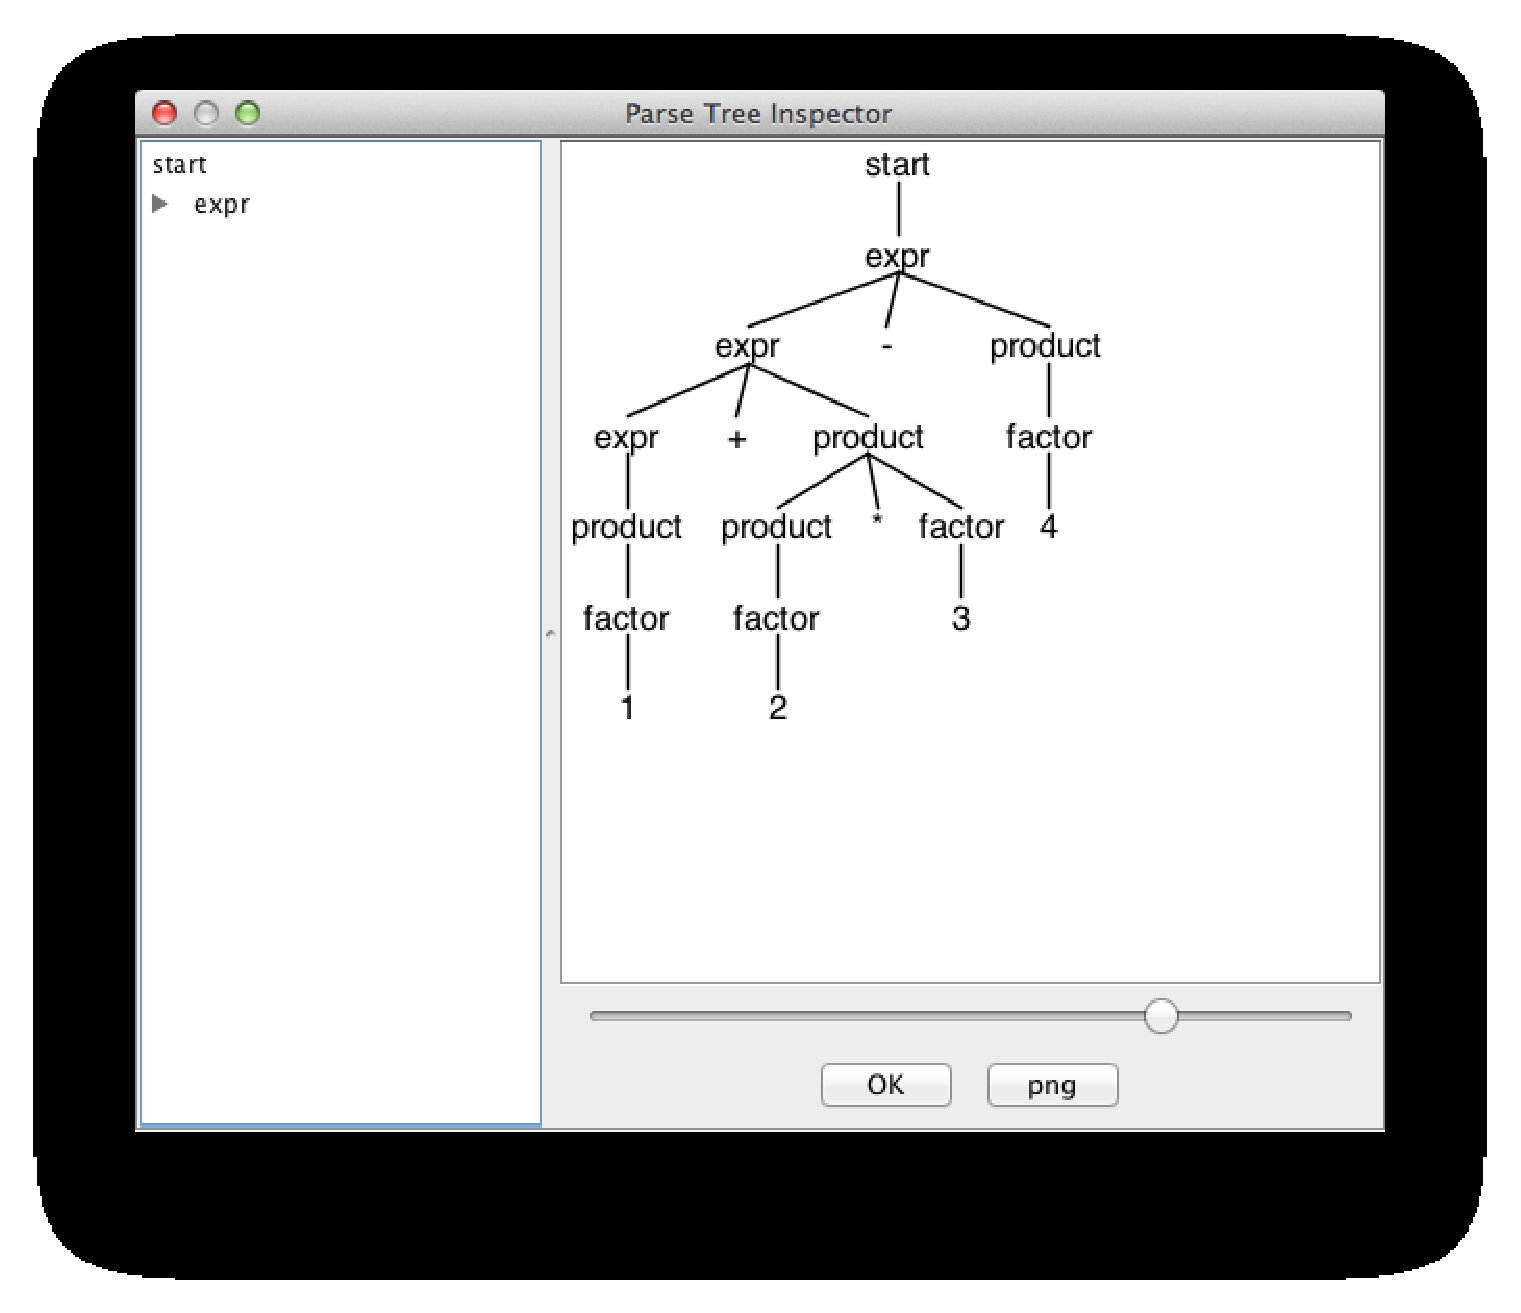
\epsfig{file=Abbildungen/expr.eps, scale=0.7}
   \caption{Syntax-Baum, der beim Parsen des Strings ``\texttt{1+2*3}'' erzeugt wird.}
  \label{fig:expr.eps}
\end{figure}



\section{Ein Parser zur Auswertung arithmetischer Ausdr\"ucke}
Das letzte Beispiel ist noch nicht sehr spektakul\"ar, weil die vom Parser erkannten
Ausdr\"ucke nicht ausgewertet werden.  Wir pr\"asentieren jetzt ein komplexeres Beispiel, bei
dem arithmetische Ausdr\"ucke ausgewertet und die erhaltenen Ergebnisse in Variablen
gespeichert werden k\"onnen.  Wir gehen dabei in zwei Schritten vor und pr\"asentieren
zun\"achst eine reine Grammatik in \textsc{Antlr}-Notation.  Anschlie{\ss}end erweitern wir diese
mit Aktionen, in denen die Ausdr\"ucke ausgewertet werden k\"onnen.
Abbildung \ref{fig:Program.g4} zeigt diese Grammatik.  Gegen\"uber der vorher gezeigten
Grammatik f\"ur arithmetische Ausdr\"ucke gibt es die folgenden \"Anderungen:

\begin{figure}[!ht]
\centering
\begin{Verbatim}[ frame         = lines, 
                  framesep      = 0.3cm, 
                  labelposition = bottomline,
                  numbers       = left,
                  numbersep     = -0.2cm,
                  xleftmargin   = 0.8cm,
                  xrightmargin  = 0.8cm,
                ]
    grammar Program;
    
    program : stmnt+ ;
    
    stmnt   : ID ':=' expr ';'
            | expr ';'
            ;    
    
    expr    : expr ('+'|'-') product
            | product
            ;
    
    product : product ('*'|'/') factor
            | factor
            ;
    
    factor  : '(' expr ')'
            | ID
            | INT
            ;
    
    ID : [a-zA-Z][a-zA-Z0-9]*;
    INT: '0'|[1-9][0-9]*;
    WS : [ \v\t\n\r] -> skip; 
\end{Verbatim}
\vspace*{-0.3cm}
\caption{Eine Grammatik f\"ur die Auswertung von Ausdr\"ucken.}
\label{fig:Program.g4}
\end{figure}


\begin{enumerate}
\item Das Start-Symbol ist jetzt \texttt{program}.  Es steht f\"ur eine Liste
      von Zuweisungen der folgenden Form:
      \\[0.2cm]
      \hspace*{1.3cm}
      $\textsl{var} \;\mathtt{:=}\; \textsl{expr}\mathtt{;}$
      \\[0.2cm]
      Hier ist \texttt{var} der Name einer Variablen und \textsl{expr} ist ein
      arithmetischer Ausdruck.
\item \texttt{stmnt} bezeichnet eine Zuweisung oder einen einzelnen Ausdruck.
\item Wir haben die Regeln f\"ur die syntaktischen Variablen \textsl{expr} und \textsl{product}
      vereinfacht, indem wir jeweils die beiden Operatoren ``\texttt{+}'' und ``\texttt{-}'' bzw.
      \squoted{*} und \squoted{/} zusammengefasst haben.
      Da \textsc{Antlr} \textsc{Ebnf}-Grammatiken unterst\"utzt, k\"onnen wir f\"ur \textsl{expr}
      beispielsweise die Regel
      \\[0.2cm]
      \hspace*{1.3cm}
      \texttt{expr : expr ('+'|'-') product | product ;}
      \\[0.2cm]
      verwenden.  Die Grammatik-Regel f\"ur \textsl{product} haben wir in \"ahnlicher Weise
      ge\"andert.
\item Das Terminal \texttt{ID} bezeichnet den Namen einer Variablen.  Ein solcher Name
      besteht aus einer beliebigen Folge von Buchstaben und Ziffern, die mit einem Buchstaben 
      beginnen muss.
\end{enumerate}
Mit diesem Parser k\"onnen wir jetzt zum Beispiel die folgende Eingabe parsen:
\begin{verbatim}
    x = 2 * 3; y = 4 * 5; z = x * x + y * y; 
    z / 3;
\end{verbatim}
Wir wollen nun einen ganz einfachen Interpreter entwickeln, der eine Folge von solchen
Zuweisungen auswertet und die bei der Auswertung berechneten Zwischen-Ergebnisse
in Variablen abspeichert, auf die in folgenden Ausdr\"ucken Bezug genommen werden kann.
Weiterhin soll jeder Ausdruck, der keiner Variablen zugewiesen wird, ausgewertet und
ausgegeben werden.  Abbildung \ref{fig:Program.g4-2} zeigt die Realisierung eines solchen
Interpreters mit \textsc{Antlr}.

\begin{figure}[!ht]
\centering
\begin{Verbatim}[ frame         = lines, 
                  framesep      = 0.3cm, 
                  labelposition = bottomline,
                  numbers       = left,
                  numbersep     = -0.2cm,
                  xleftmargin   = 0.3cm,
                  xrightmargin  = 0.3cm,
                ]
    grammar Program;
     
    @header {
        import java.util.TreeMap;
    }
    
    @members {
        TreeMap<String, Integer> varTable = new TreeMap<String, Integer>();
    }
    
    program : stmnt+ ;
    
    stmnt : ID ':=' expr ';' { varTable.put($ID.text, $expr.result); }
          |         expr ';' { System.out.println($expr.result);     }
          ;    
    
    expr returns [int result]
        : e = expr { $result = $e.result; }
          (   '+' p = product { $result += $p.result; }
            | '-' p = product { $result -= $p.result; }
          )
        | p = product { $result = $p.result; }
        ;
    
    product returns [int result]
        : p = product { $result = $p.result; }
          (
              '*' f = factor { $result *= $f.result; }
            | '/' f = factor { $result /= $f.result; }
          )
        | f = factor { $result = $f.result; }
        ;
    
    factor returns [int result]
        : '(' expr ')' { $result = $expr.result;           }
        | ID           { $result = varTable.get($ID.text); }
        | INT          { $result = new Integer($INT.text); }
        ;
    
    ID : [a-zA-Z][a-zA-Z0-9]*;
    INT: '0'|[1-9][0-9]*;
    WS : [ \v\t\n\r] -> skip; 
\end{Verbatim} 
%\$
\vspace*{-0.3cm}
\caption{Ein Interpreter zur Auswertung von Ausdr\"ucken.}
\label{fig:Program.g4-2}
\end{figure}

\begin{enumerate}
\item Da wir die Werte der einzelnen Variablen in einer Tabelle abspeichern m\"ussen,
      importieren wir in den Zeilen 3 -- 5 die Klasse \texttt{java.util.TreeMap}, denn
      diese Klasse implementiert Tabellen effizient als bin\"are B\"aume.

      Allgemein setzt \textsc{Antlr} all den Code, der durch das Schl\"usselwort
      ``\texttt{@header}'' spezifiert wird, an den Anfang der erstellten Parser-Datei.
\item In den Zeilen 7 -- 9 definieren wir zus\"atzliche Member-Variablen f\"ur die erzeugte
      Klasse \texttt{ProgramParser}.  In unserem Fall definieren wir hier die Tabelle, die
      sp\"ater die Werte der Variablen enth\"alt, als Abbildung, die Strings ganze Zahlen zuordnet.

      Allgemein setzt \textsc{Antlr} all den Code, der durch das Schl\"usselwort
      ``\texttt{@members}'' spezifiert wird, an den Anfang der erstellten Parser-Klasse.
      Dieses Feature kann sowohl zur Definition von zus\"atzlichen Klassen-Variablen als auch
      von Methoden verwendet werden.
      
      Wir reichern nun die Grammatik-Regeln mit Aktionen an, die durchgef\"uhrt werden, wenn
      der Parser die entsprechende Grammatik-Regel anwendet.  Die Aktionen werden von der
      eigentlichen Grammatik-Regel, f\"ur die sie angewendet werden sollen, dadurch
      abgesetzt, dass sie in den geschweiften Klammern ``\texttt{\{}'' und ``\texttt{\}}''
      eingefasst werden.
\item Wird vom Parser in Zeile 13 eine Zuweisung der Form $\textsl{var} \;\mathtt{:=}\; \textsl{expr}$
      erkannt,  
      so soll der Wert des Ausdrucks \textsl{expr} berechnet und das Ergebnis in der
      Tabelle \texttt{varTable} unter dem Namen \textsl{var} eingetragen werden.
      In der Grammatik-Regel
      \\[0.2cm]
      \hspace*{1.3cm}
      \textsl{stmnt} $\rightarrow$ \texttt{ID} ':=' \textsl{expr} ';'
      \\[0.2cm]
      haben wir einerseits das Token \texttt{ID}, auf dessen Namen wir mit \texttt{\symbol{36}ID.text}
      zugreifen k\"onnen, andererseits haben wir die syntaktische Variable \textsl{expr}.
      Wir werden sp\"ater dieser syntaktischen Variable die \textsl{Java}-Variable
      \texttt{result} als Ergebnis-Variable zuordnen, die den zugeh\"origen Wert enth\"alt.  
      Dann k\"onnen wir mit
      \texttt{\symbol{36}expr.result} auf diesen Wert zugreifen.

      In Zeile 14 haben wir einen einzelnen arithmetischen Ausdruck, den wir auswerten und ausgeben.
\item In Zeile 17 definieren wir mit der Zeile
      \\[0.2cm]
      \hspace*{1.3cm}
      \texttt{expr returns [int result]}
      \\[0.2cm]
      dass die Methode, die eine \textsl{expr} parst, als Ergebnis ein \texttt{int} zur\"uck
      gibt und dass dieses in der Variable mit dem Namen \texttt{result} abgespeichert wird.
\item In der Grammatik-Regel
      \\[0.2cm]
      \hspace*{1.3cm}
      \texttt{expr : expr ('+'|'-') product | product ;}
      \\[0.2cm]
      haben wir in Zeile 18 -- 20 den verschiedenen Auftreten der syntaktischen Variablen
      \texttt{expr} und \texttt{product} die Namen $e$ und $p$ zugeordnet, auf die wir dann in den
      Aktionen zugreifen k\"onnen.  In den Aktionen muss diesen Variablen allerdings ein Dollar-Zeichen
      vorgestellt werden.

      Die Aktionen selber bestehen nun darin, dass wir der Variablen \texttt{result}
      das Ergebnis der jeweiligen Berechnung zuweisen.
\item In den Zeilen 36 und 37 greifen wir auf die Strings, die den Token
      \texttt{ID} und \texttt{INT} entsprechen, mit Hilfe der f\"ur Token vordefinierten
      Variable \texttt{text} zur\"uck.  Beachten Sie, dass wir in Zeile 36 den Wert, der zu einer
      Variablen in der Tabelle \texttt{varTable} gespeichert ist, auslesen und als Ergebnis zur\"uck
      geben. 
\end{enumerate}

\section{Erzeugung abstrakter Syntax-B\"aume}
Bei der Auswertung arithmetischer Ausdr\"ucke im letzten Abschnitt hatten wir Gl\"uck
und konnten das Ergebnis eines Ausdrucks unmittelbar mit Hilfe von semantischen Aktionen
berechnen.  Bei komplexeren Problemen ist es in der Regel erforderlich, zun\"achst einen
abstrakten Syntax-Baum zu erzeugen.  Die eigentliche Berechnung findet dann erst nach dem
Parsen auf dem Syntax-Baum statt.  Wir wollen dieses Verfahren an einem Beispiel
demonstrieren.  Bei dem Beispiel geht es wieder um die symbolische Differentiation
arithmetischer Ausdr\"ucke.  Ist beispielsweise der arithmetische Ausdruck 
\[ x \cdot \ln(x) \]
gegeben, so findet sich f\"ur die Ableitung dieses Ausdrucks nach der Variable $x$ mit Hilfe
der Produkt-Regel das
Ergebnis 
\[ 1 \cdot \ln(x) + x \cdot \frac{1}{x}. \]  
Da die arithmetischen Ausdr\"ucke nun
zus\"atzlich zu den Operatoren, welche die vier Grundrechenarten beschreiben, auch noch 
Funktionszeichen f\"ur die Exponential-Funktion und den nat\"urlichen Logarithmus enthalten
sollen, m\"ussen wir die Grammatik aus dem letzten Abschnitt erweitern.
Abbildung \ref{fig:Expr-exp-ln} zeigt die entsprechend erweiterte EBNF-Grammatik.

\begin{figure}[htbp]
  \begin{center}    
  \framebox{
  \framebox{
  \begin{minipage}[t]{9cm}

  \begin{eqnarray*}
  \textsl{expr}   & \rightarrow & \;\textsl{expr}\;\;(\quoted{+}|\quoted{-})  \;\; \textsl{product}  \\
                  & \mid        & \textsl{product}                                 \\[0.2cm]
  \textsl{product} & \rightarrow & \;\textsl{product}\;\;\;\;(\quoted{*}|\quoted{/}) \;\; \textsl{factor} \\
                  & \mid        & \textsl{factor}  \\[0.2cm]
  \textsl{factor} & \rightarrow & \quoted{(} \textsl{expr} \quoted{)}              \\
                  & \mid        & \quoted{exp} \quoted{(} \textsl{expr} \quoted{)} \\
                  & \mid        & \quoted{log} \quoted{(} \textsl{expr} \quoted{)} \\
                  & \mid        & \;\textsc{Variable}                              \\
                  & \mid        & \;\textsc{Number} 
  \end{eqnarray*}
  \vspace*{-0.5cm}

  \end{minipage}}}
  \end{center}
  \caption{EBNF-Grammatik f\"ur arithmetische Ausdr\"ucke mit Exponential-Funktion und Logarithmus.}
  \label{fig:Expr-exp-ln}
\end{figure}

\subsection{Implementierung des Parsers}
Abbildung \ref{fig:grammatik.g} zeigt die \textsc{Antlr}-Implementierung der Grammatik
aus Abbildung \ref{fig:Expr-exp-ln}.  

\begin{figure}[!ht]
\centering
\begin{Verbatim}[ frame         = lines, 
                  framesep      = 0.3cm, 
                  labelposition = bottomline,
                  numbers       = left,
                  numbersep     = -0.2cm,
                  xleftmargin   = 0.0cm,
                  xrightmargin  = 0.0cm,
                ]
    grammar Expr;
    
    expr returns [Expr result]
        : e = expr '+' p = product { $result = new Sum(       $e.result, $p.result); }
        | e = expr '-' p = product { $result = new Difference($e.result, $p.result); }
        | p = product              { $result = $p.result; }    
        ;
    
    product returns [Expr result]
        : p = product '*' f = factor { $result = new Product( $p.result, $f.result); }
        | p = product '/' f = factor { $result = new Quotient($p.result, $f.result); }
        | f = factor                 { $result = $f.result; }
        ;
    
    factor returns [Expr result]
        : '(' expr ')'       { $result = $expr.result;                  }
        | 'exp' '(' expr ')' { $result = new Exponential($expr.result); }
        | 'log' '(' expr ')' { $result = new Logarithm(  $expr.result); }
        | VAR                { $result = new Variable($VAR.text);       }
        | NUM                { $result = new Number($NUM.text);         }
        ;
    
    VAR : [a-zA-Z][a-zA-Z0-9]*;
    NUM : '0'|[1-9][0-9]*;
    WS  : [ \v\t\n\r] -> skip; 
\end{Verbatim}
\vspace*{-0.3cm}
\caption{Die \textsc{Antlr}-Spezifikation der Grammatik.}
\label{fig:grammatik.g}
\end{figure}

\begin{enumerate}
\item In Zeile 3 deklarieren wir durch ``\texttt{returns [Expr result]}'',
      dass beim Erkennen einer \textsl{expr} nun ein Objekt der Klasse \texttt{Expr}
      zur\"uck gegeben werden soll und dass dieses Objekt \"uber den Namen
      \texttt{result} angesprochen werden kann.  Die Klasse \texttt{Expr} ist hier eine abstrakte
      Klasse, von der wir die Klassen
      \begin{enumerate}
      \item \texttt{Sum} (zur Darstellung von Termen der Form $s + t$),
      \item \texttt{Difference} (zur Darstellung von Termen der Form $s - t$),
      \item \texttt{Product} (zur Darstellung von Termen der Form $s * t$),
      \item \texttt{Quotient} (zur Darstellung von Termen der Form $s / t$),
      \item \texttt{Exponential} (zur Darstellung von Termen der Form $\textsl{exp}(s)$),
      \item \texttt{Logarithm} (zur Darstellung von Termen der Form $\textsl{ln}(s)$),
      \item \texttt{Number} (zur Darstellung von Zahlen) und
      \item \texttt{Variable} (zur Darstellung von Variablen)
      \end{enumerate}
      ableiten.  Die Klasse \texttt{Expr} besitzt nur die abstrakte Methode 
      \\[0.2cm]
      \hspace*{1.3cm}
      \texttt{public abstract Expr diff(String x);}
      \\[0.2cm]
      die dazu benutzt wird, einen arithmetischen Ausdruck nach einer gegebenen Variablen
      abzuleiten.  Die von \texttt{Expr} abgeleiteten Klassen sind alle nach dem gleichen Muster
      aufgebaut.  Beispielhaft zeigt Abbildung \ref{fig:Product.java} auf Seite \pageref{fig:Product.java}
        die Implementierung der Klasse 
      \texttt{Product}.
      \begin{enumerate}
      \item Die Klasse beinhaltet die beiden Member-Variablen \texttt{mLhs} und \texttt{mRhs}.
            Ein Objekt der Klasse \texttt{Product} wird als das Produkt
            \\[0.2cm]
            \hspace*{1.3cm}
            $\mathtt{mLhs} * \mathtt{mRhs}$
            \\[0.2cm]
            interpretiert.
      \item Zus\"atzlich gibt es eine Implementierung der Methode \texttt{diff}, in der die
            Produkt-Regel umgesetzt wird.
      \item Zur Ausgabe ist weiterhin eine \texttt{toString}-Methode vorhanden.
      \end{enumerate}

\begin{figure}[!ht]
\centering
\begin{Verbatim}[ frame         = lines, 
                  framesep      = 0.3cm, 
                  firstnumber   = 1,
                  labelposition = bottomline,
                  numbers       = left,
                  numbersep     = -0.2cm,
                  xleftmargin   = 0.0cm,
                  xrightmargin  = 0.0cm,
                ]
    public class Product extends Expr {
        private Expr mLhs;
        private Expr mRhs;
    
        public Product(Expr lhs, Expr rhs) {
            mLhs = lhs;
            mRhs = rhs;
        }
        public Expr diff(String x) {
            return new Sum(new Product(mLhs.diff(x), mRhs), new Product(mLhs, mRhs.diff(x)));
        }
        public String toString() {
            return mLhs.toString() + " * " + mRhs.toString();
        }
    }
\end{Verbatim}
\vspace*{-0.3cm}
\caption{Die Klasse \texttt{Product} zur Darstellung von Produkten.}
\label{fig:Product.java}
\end{figure}

      
      
\item In Zeile 4 haben wir zun\"achst ein Produkt erkannt, dass wir unter der Variable
      $p$ abspeichern.  Anschlie{\ss}end weisen wir der Variable \texttt{result} dieses
      Produkt zu.  Falls nun sp\"ater noch ein ``\texttt{+}''-- oder ``\texttt{-}''
      Zeichen gefolgt von einem weiteren Ausdruck gelesen wird, so bauen wir aus dem neu
      gelesenen Ausdruck und dem alten Wert von \texttt{result} den neuen Wert von
      \texttt{result}.  Dies kann mehrmals passieren, da dieser Teil der Grammatik-Regel
      in $( \cdots )*$ eingeschlossen ist.
      
      Beispielsweise wird ein Ausdruck der Form
      \\[0.2cm]
      \hspace*{1.3cm}
      $p_1 + p_2 + p_3$
      \\[0.2cm]
      \"ubersetzt in ein Java-Objekt der Form
      \\[0.2cm]
      \hspace*{1.3cm}
      $\texttt{new\ Sum}(\texttt{new\ Sum}(p_1, p_2), p_3))$.       
\item Die weiteren Grammatik-Regeln erzeugen in analoger Weise \textsl{Java}-Objekte.
\end{enumerate}

Zum Abschluss zeigt Abbildung \ref{fig:Differentiate.java} noch die Einbindung des Parsers.
Gegen\"uber dem in Abbildung \ref{fig:ParseExpr.java} gezeigten Treiber gibt es nur einen
wesentlichen Unterschied: In Zeile 20 wird nun ein Objekt der Klasse \texttt{Expr} erzeugt.
Beachten Sie, dass der Aufruf
\\[0.2cm]
\hspace*{1.3cm}
\texttt{parser.expr()}
\\[0.2cm]
zun\"achst ein Objekt der Klasse \texttt{ExprParser.ExprContext} erzeugt.  Bei dieser Klasse handelt
es sich um eine innere Klasse der Klasse \texttt{ExprParser}.  Die innere Klasse
\texttt{ExprContext} enth\"alt nun eine Member-Variable mit dem Namen \texttt{result}, in der die
eigentliche \texttt{Expr} gespeichert ist.  
F\"ur dieses Objekt rufen wir dann in Zeile 21 die Methode $\textsl{diff}()$ auf, welche die
symbolische Ableitung berechnet.


\begin{figure}[!ht]
\centering
\begin{Verbatim}[ frame         = lines, 
                  framesep      = 0.3cm, 
                  labelposition = bottomline,
                  numbers       = left,
                  numbersep     = -0.2cm,
                  xleftmargin   = 0.8cm,
                  xrightmargin  = 0.8cm,
                ]
    import org.antlr.v4.runtime.*;
    import java.io.FileInputStream;
    import java.io.InputStream;
    
    public class Differentiate {
    
        public static void main(String[] args) throws Exception {
            String inputFile = null; 
            if (args.length > 0) { 
    	    inputFile = args[0];
    	}
            InputStream is = System.in;
            if (inputFile != null) {
    	    is = new FileInputStream(inputFile);
    	}
            ANTLRInputStream  input  = new ANTLRInputStream(is);
            ExprLexer         lexer  = new ExprLexer(input);
            CommonTokenStream ts     = new CommonTokenStream(lexer);
            ExprParser        parser = new ExprParser(ts);
            Expr expr = parser.expr().result;
            Expr diff = expr.diff("x");
            System.out.println("d (" + expr + ")/dx = " + diff);
        }
    }
\end{Verbatim}
\vspace*{-0.3cm}
\caption{Ein Treiber f\"ur den Parser.}
\label{fig:Differentiate.java}
\end{figure}
\pagebreak


\exerciseEng
The \href{https://github.com/karlstroetmann/Formal-Languages}{github directory} associated with this lecture
contains the file
\\[0.2cm]
\hspace*{1.3cm}
\href{https://github.com/karlstroetmann/Formal-Languages/tree/master/Exercises/Grammar2HTML-Antlr/c-grammar.g}{
\texttt{Exercises/Grammar2HTML-Antlr/c-grammar.g}}
\\[0.2cm]
that specifies the syntax of the programming language 
\href{https://en.wikipedia.org/wiki/C_(programming_language)}{\texttt{C}}.

\begin{enumerate}[(a)]
\item Your first task is specify the syntax used to denote the grammar rules given in the file
      \texttt{c-grammar.g}.  Of course, in order to specify this syntax you should use a
      context-free grammar. 
\item Next, you should develop a parser that is capable of reading the file \texttt{c-grammar.g}
      and that, furthermore, can convert this grammar into \textsc{Html}. 
      This parser should be developed using the tool \textsc{Antlr}.
\end{enumerate}

\remarkEng
\begin{enumerate}
\item The directory 
      \\[0.2cm]
      \hspace*{1.3cm}
      \href{https://github.com/karlstroetmann/Formal-Languages/tree/master/Exercises/Grammar2HTML/}{\texttt{Exercises/Grammar2HTML}}
      \\[0.2cm]
      contains several classes that represent various nodes of an abstract syntax tree corresponding to a
      given grammar.  The given classes already contain an implementation of the method $\texttt{toString}()$. This method 
      converts a node of the abstract syntax tree into an \textsc{Html} string.
\item \textsc{Antlr} provides a negation operator that is written as ``\texttt{\symbol{126}}''.
      Using the negation operator comes in handy when recognizing \emph{literal tokens},  
      i.e.~tokens that represent either keywords or operators of the language \texttt{C}.  In the
      file \texttt{c-grammar.g}, literal tokens are enclosed in single quotes.
\item For obscure historical reasons, \textsc{Antlr} treats the string ``\texttt{rule}'' as a 
      keyword.  Therefore, it is not possible to have a syntactical variable that is called
      ``\texttt{rule}''. 
\end{enumerate}



%%% Local Variables: 
%%% mode: latex
%%% TeX-master: "formal-languages"
%%% End: 

\section{Implementing a Simple Interpreter  \label{chapter:interpreter}}

\textsc{Antlr} supports \textsc{Ebnf} grammars. For example, the postfix operators
``\texttt{*}'', ``\texttt{+}'' and ``\texttt{?}'' known from regular expressions are
supported. We demonstrate the use of these operators by developing an interpreter for a
simple programming language using the parser generator \textsc{Antlr}. Figure
\ref{fig:Pure.g4} shows the \textsc{Antlr} grammar of the programming language for which
we are developing an interpreter in this section. The syntax of this language is modeled
after the syntax of the language \texttt{C}, but instead of the simple equality sign
``\texttt{=}'', we use the string ``\texttt{:=}'' as the assignment operator.

\begin{figure}[!ht]
\centering
\begin{Verbatim}[ frame         = lines, 
                  framesep      = 0.3cm, 
                  firstnumber   = 1,
                  labelposition = bottomline,
                  numbers       = left,
                  numbersep     = -0.2cm,
                  xleftmargin   = 0.8cm,
                  xrightmargin  = 0.8cm,
                ]
    grammar Pure;
    
    program  : statement+
             ;  
    statement: VAR ':=' expr ';'
             | 'print' '(' expr ')' ';'
             | 'if'    '(' boolExpr ')' '{' statement* '}'
             | 'while' '(' boolExpr ')' '{' statement* '}'
             ;
    boolExpr : expr '==' expr
             | expr '<'  expr
             ;
    expr     : expr '+' product
             | expr '-' product
             | product
             ;
    product  : product '*' factor
             | product '/' factor
             | factor
             ;
   factor    : 'read' '(' ')' 
             | '(' expr ')'
             | VAR
             | NUMBER
             ;
    VAR      : [a-zA-Z][a-zA-Z_0-9]*;
    NUMBER   : '0'|[1-9][0-9]*;
    
    MULTI_COMMENT : '/*' .*? '*/' -> skip;
    LINE_COMMENT  : '//' ~('\n')* -> skip;
    WS            : [ \t\n\r]     -> skip; 
\end{Verbatim}
\vspace*{-0.3cm}
\caption{\textsc{Antlr}-Grammatik f\"ur eine einfache Programmier-Sprache.}
\label{fig:Pure.g4}
\end{figure}

The commands of the language to be implemented include assignments, print commands,
\texttt{if} statements, and \texttt{while} loops. Figure \ref{fig:sum.sl} shows
an example program that conforms to this grammar. This program first reads a number
which is stored in the variable \texttt{n}. Subsequently, the sum
\[
\hspace*{1.3cm}
\ds\sum\limits_{\mbox{$\normalsize i=1$}}^{\mbox{$\normalsize n^2$}} \mbox{\Large $i$}
\]
is computed and printed using a \texttt{while} loop.

\begin{figure}[!ht]
\centering
\begin{Verbatim}[ frame         = lines, 
                  framesep      = 0.3cm, 
                  labelposition = bottomline,
                  numbers       = left,
                  numbersep     = -0.2cm,
                  xleftmargin   = 0.8cm,
                  xrightmargin  = 0.8cm,
                ]
    n := read();
    s := 0;
    i := 0;
    while (i < n * n) {
        i := i + 1;
        s := s + i;
    }
    print(s);
\end{Verbatim}
\vspace*{-0.3cm}
\caption{Ein Programm zur Berechnung der Summe $\sum\limits_{i=0}^{n^2} i$.}
\label{fig:sum.sl}
\end{figure}
\FloatBarrier

Similar to our program for symbolic differentiation, we will represent the individual commands as
nested tuples. The program shown in Figure \ref{fig:sum.sl} is represented by the nested tuple displayed in
Figure \ref{fig:sum.ast}. This nested tuple is nothing other than the abstract syntax tree
corresponding to the original program. 

\begin{figure}[!ht]
\centering
\begin{Verbatim}[ frame         = lines, 
                  framesep      = 0.3cm, 
                  labelposition = bottomline,
                  numbers       = left,
                  numbersep     = -0.2cm,
                  xleftmargin   = 0.8cm,
                  xrightmargin  = 0.8cm,
                ]
    ('program',
        ('read', 'n'),
        (':=', 's', 0),
        (':=', 'i', 0),
        ('while', ('<',  'i', ('*', 'n', 'n')),
            (':=', 'i', ('+', 'i', 1)),
            (':=', 's', ('+', 's', 'i'))
        ),
        ('print', 's')
    )
\end{Verbatim}
\vspace*{-0.3cm}
\caption{A nested tuple that represents the program from Figure \ref{fig:sum.sl}.}
\label{fig:sum.ast}
\end{figure}

\begin{figure}[!ht]
\centering
\begin{Verbatim}[ frame         = lines, 
                  framesep      = 0.3cm, 
                  labelposition = bottomline,
                  numbers       = left,
                  numbersep     = -0.3cm,
                  xleftmargin   = -0.3cm,
                  xrightmargin  = 0.0cm,
                ]
    grammar Simple;
    
    program returns [stmnt_list] 
        : {SL = ['program']} (s = statement {SL.append($s.stmnt)})+ {$stmnt_list = tuple(SL)}
        ;
    
    statement returns [stmnt]
        : v = VAR ':=' e = expr ';'       {$stmnt = (':=', $v.text, $e.result)}
        | 'print' '(' r = expr ')' ';'    {$stmnt = ('print', $r.result)}
        | 'if' '(' b = boolExpr ')' {SL = []} '{' (l = statement {SL.append($l.stmnt)})* '}' 
          {$stmnt = ('if', $b.result) + tuple(SL)}
        | 'while' '(' b = boolExpr ')' {SL = []} '{' (l = statement {SL.append($l.stmnt)})* '}' 
          {$stmnt = ('while', $b.result) + tuple(SL)}
        ;
    
    boolExpr returns [result]
        : l = expr '==' r = expr {$result = ('==', $l.result, $r.result)} 
        | l = expr '<'  r = expr {$result = ('<',  $l.result, $r.result)}
        ;
    
    expr returns [result]
        : e = expr '+' p = product {$result = ('+', $e.result, $p.result)}
        | e = expr '-' p = product {$result = ('-', $e.result, $p.result)}
        | p = product              {$result = $p.result}
        ;
    
    product returns [result]
        : p = product '*' f = factor {$result = ('*', $p.result, $f.result)}
        | p = product '/' f = factor {$result = ('/', $p.result, $f.result)}
        | f = factor                 {$result = $f.result}
        ;
    
    factor returns [result]
        : 'read' '(' ')' {$result = ('read',)}
        | '(' expr ')'   {$result = $expr.result}
        | v = VAR        {$result = $v.text}
        | n = NUMBER     {$result = int($n.text)}
        ;
    
    VAR    : [a-zA-Z][a-zA-Z_0-9]*;
    NUMBER : '0'|[1-9][0-9]*;
    
    MULTI_COMMENT : '/*' .*? '*/' -> skip;
    LINE_COMMENT  : '//' ~('\n')* -> skip;
    WS            : [ \t\n\r]     -> skip;
\end{Verbatim}
\vspace*{-0.3cm} %\$
\caption{\textsc{Antlr}-Spezifikation der Grammatik.}
\label{fig:Simple.g}
\end{figure}

\noindent
Figure \ref{fig:Simple.g} shows the implementation of the parser using the
\textsc{Antlr} tool.
\begin{enumerate}
\item The start symbol of the grammar is the variable \texttt{program}.
      When parsing this variable, the parser returns a tuple of commands in the variable
      \texttt{stmnt\_list}.
      To this end, we initialize the variable \texttt{SL}
      as a list containing only the string \texttt{'program'}. Subsequently, each recognized command
      is appended to this list. Finally, this list is converted into a tuple and stored in the
      attribute variable \texttt{stmnt\_list}.
\item The syntactic variable \texttt{statement} describes the various commands that 
      are supported in our simple language.
      \begin{enumerate}[(a)]
      \item The simplest commands are the assignments. These have the form:
            \\[0.2cm]
            \hspace*{1.3cm}
            $v \;\texttt{:=}\; e \texttt{;}$
            \\[0.2cm]
            Here, $v$ is a variable and $e$ is an arithmetic expression.
            Such an assignment is represented by the nested tuple
            \\[0.2cm]
            \hspace*{1.3cm}
            $(\texttt{':='}, v, e)$.
      \item The command for printing a value has the form:
            \\[0.2cm]
            \hspace*{1.3cm}
            $\texttt{print(} e \texttt{);}$
            \\[0.2cm]
            The purpose of this command is to compute the value of the expression $e$ and print it.
            This command is represented by the nested tuple
            \\[0.2cm]
            \hspace*{1.3cm}
            $(\texttt{'print'}, v)$.
      \item A conditional test has the syntax:
            \\[0.2cm]
            \hspace*{1.3cm}
            $\texttt{if}\; \texttt{(}\; b\; \texttt{)}\; \texttt{\{}\; \textsl{statements}\; \texttt{\}}$
            \\[0.2cm]
            Here, $b$ is an expression that evaluates to \texttt{True} or \texttt{False}
            and \texttt{statements} is a list of commands that are executed if
            $b$ evaluates to \texttt{True}.
            This command is represented by the nested tuple
            \\[0.2cm]
            \hspace*{1.3cm}
            $(\texttt{'if'}, b, \textsl{statements})$.
            \\[0.2cm]
            Here, $b$ is a nested tuple representing the Boolean expression.
      \item A loop has the syntax:
            \\[0.2cm]
            \hspace*{1.3cm}
            $\texttt{while}\; \texttt{(}\; b\; \texttt{)}\; \texttt{\{}\; \textsl{statements}\; \texttt{\}}$.
            \\[0.2cm]
            Here, $b$ is an expression that evaluates to \texttt{True} or \texttt{False}
            and \texttt{statements} is a list of commands that are executed as long as
            $b$ evaluates to \texttt{True}.
            This command is represented by the nested tuple
            \\[0.2cm]
            \hspace*{1.3cm}
            $(\texttt{'while'}, b, \textsl{statements})$.
      \end{enumerate}
\item The syntactic variable \texttt{boolExpr} describes an expression that takes a Boolean value.
      There are two ways to generate such a value.
      \begin{enumerate}
      \item An expression of the form
            \\[0.2cm]
            \hspace*{1.3cm}
            $l \;\texttt{==}\; r $
            \\[0.2cm]
            tests whether the evaluations of $l$ and $r$ yield the same values.
            This expression is represented by the nested tuple
            \\[0.2cm]
            \hspace*{1.3cm}
            $(\texttt{'=='}, l, r)$.
      \item An expression of the form
            \\[0.2cm]
            \hspace*{1.3cm}
            $l \;\texttt{<}\; r $
            \\[0.2cm]
            tests whether the evaluation of $l$ yields a value that is smaller than the
            value obtained from the evaluation of $r$. 
            This expression is represented by the nested tuple
            \\[0.2cm]
            \hspace*{1.3cm}
            $(\texttt{'<'}, l, r)$
      \end{enumerate}
\item In a similar manner, the syntactic variables \texttt{expr}, \texttt{product}, and \texttt{factor}
      describe arithmetic expressions.
      Since we have already discussed this in sufficient detail earlier, we will not delve further into
      the grammar rules that define these syntactic variables at this point.
\end{enumerate}
The specification of the tokens is shown in lines 40--45 of Figure \ref{fig:Simple.g}.
The scanner primarily differentiates between variables and numbers.
Variables start with an uppercase or lowercase letter, followed by additional digits and
the underscore. Sequences of digits are interpreted as numbers. If such a
sequence contains more than one character, the first digit must not be 0. Additionally, the
scanner removes whitespace and comments. We have also used the so-called \emph{non-greedy} version of the
operator ``\texttt{*}'' in the specification of multiline comments. The non-greedy version of the
operator ``\texttt{*}'' is written as ``\texttt{*?}'' and matches as little as possible. Therefore, the regular expression
\[
\hspace*{1.3cm}
\texttt{'/*' .*? '*/'}
\]
represents a string that starts with the character sequence ``\texttt{/*}'', ends with the character sequence ``\texttt{*/}'',
and is as short as possible. This ensures that in a line like
\[
\hspace*{1.3cm}
\texttt{/* Hugo */ i := i + 1; /* Anton */}
\]
two separate comments are recognized.


\begin{figure}[!ht]
\centering
\begin{Verbatim}[ frame         = lines, 
                  framesep      = 0.3cm, 
                  firstnumber   = 1,
                  labelposition = bottomline,
                  numbers       = left,
                  numbersep     = -0.2cm,
                  xleftmargin   = 0.0cm,
                  xrightmargin  = 0.0cm,
                ]
    def main(file):
        with open(file, 'r') as handle:
            program_text = handle.read()
        input_stream  = antlr4.InputStream(program_text)
        lexer         = SimpleLexer(input_stream)
        token_stream  = antlr4.CommonTokenStream(lexer)
        parser        = SimpleParser(token_stream)
        result        = parser.program()
        Statements    = result.stmnt_list
        execute_tuple(Statements)
\end{Verbatim}
\vspace*{-0.3cm}
\caption{Die Funktion \texttt{main}.}
\label{fig:Interpreter.ipynb:main}
\end{figure}

\begin{figure}[!ht]
\centering
\begin{Verbatim}[ frame         = lines, 
                  framesep      = 0.3cm, 
                  firstnumber   = 1,
                  labelposition = bottomline,
                  numbers       = left,
                  numbersep     = -0.2cm,
                  xleftmargin   = 0.0cm,
                  xrightmargin  = 0.0cm,
                ]
    def execute_tuple(Statement_List, Values={}):
        for stmnt in Statement_List:
            execute(stmnt, Values)
    
    def execute(stmnt: NestedTuple, Values: dict[str, Number]) -> None:
        match stmnt:
            case 'program':
                pass
            case (':=', var, value):
                Values[var] = evaluate(value, Values)
            case ('print', expr):
                print(evaluate(expr, Values))
            case ('if', test, *SL):
                if evaluate(test, Values):
                    execute_tuple(tuple(SL), Values)
            case ('while', test, *SL):
                while evaluate(test, Values):
                    execute_tuple(tuple(SL), Values)
            case _:
                assert False, f'{stmnt} unexpected'
\end{Verbatim}
\vspace*{-0.3cm}
\caption{The function execute \texttt{execute}.}
\label{fig:Interpreter.ipynb:execute}
\end{figure}

Figure \ref{fig:Interpreter.ipynb:main} shows the function \texttt{main}, which receives the name of a
file containing a program in our simple programming language as input. This program is parsed and
thus transformed into the nested tuple \texttt{Statements}. The function \texttt{execute\_tuple} executes
the individual commands in the tuple \texttt{Statements}. It uses the function \texttt{execute} to
execute a single command. Figure \ref{fig:Interpreter.ipynb:execute} shows the
implementation of the function \texttt{execute}. This implementation consists mainly of a large
case distinction based on the type of command to be executed.
\begin{enumerate}
\item First, we check if \texttt{statement} is the string \texttt{'program'}, which marks the beginning of
      the program.\footnote{
        This marking is only needed for the representation of the program as an abstract syntax tree.}
      Since this is only a marker and not a real command, nothing further needs to be
      done.
\item If the command is an assignment of the form
      \\[0.2cm]
      \hspace*{1.3cm}
      \texttt{(':=', var, value)}
      \\[0.2cm]   
      then the value of the expression \texttt{value} is computed using the function \texttt{evaluate}.
      This value is then stored in the dictionary \texttt{Values} under the key \texttt{var}.
\item If the command is an operation of the form
      \\[0.2cm]
      \hspace*{1.3cm}
      \texttt{('print', expr)}
      \\[0.2cm]
      then the expression \texttt{expr} is first evaluated using the function \texttt{evaluate}.
      The resulting value is then printed.
\item If the command is of the form
      \\[0.2cm]
      \hspace*{1.3cm}
      \texttt{('if', test, $s_1$, $\cdots$, $s_n$)}
      \\[0.2cm]
      then \texttt{test} is a nested tuple representing a Boolean expression and
      \texttt{($s_1$, $\cdots$, $s_n$)} is a tuple of commands stored in the variable \texttt{SL}.
      In this case, the expression \texttt{test} is first evaluated using the function \texttt{evaluate}.
      If this evaluation yields the value \texttt{True}, then the
      commands in the tuple \texttt{SL} are executed in sequence.
\item If the command is of the form
      \\[0.2cm]
      \hspace*{1.3cm}
      \texttt{('while', test, $s_1$, $\cdots$, $s_n$)}
      \\[0.2cm]
      then \texttt{test} is a Boolean expression and \texttt{($s_1$, $\cdots$, $s_n$)}
      is a tuple of commands stored in the variable \texttt{SL}.
      In this case, the expression \texttt{test} is first evaluated using the function \texttt{evaluate}.
      If this evaluation yields the value \texttt{True}, then the
      commands in the tuple \texttt{SL} are executed in sequence.
      Then the expression \texttt{test} is evaluated again. If the result is
      \texttt{False}, then the execution of the command is finished. Otherwise,
      the commands in the list \texttt{SL} are executed as long as the evaluation of \texttt{test}
      yields \texttt{False}.
\end{enumerate}


\begin{figure}[!ht]
\centering
\begin{Verbatim}[ frame         = lines, 
                  framesep      = 0.3cm, 
                  firstnumber   = 1,
                  labelposition = bottomline,
                  numbers       = left,
                  numbersep     = -0.2cm,
                  xleftmargin   = 0.0cm,
                  xrightmargin  = 0.0cm,
                ]
    def evaluate(expr: NestedTuple, Values: dict[str, Number]) -> Number:
        match expr:
            case int():
                return expr
            case str():
                return Values[expr] 
            case ('read',):
                return int(input('Please enter a natural number: '))
            case ('==', lhs, rhs):
                return evaluate(lhs, Values) == evaluate(rhs, Values)
            case ('<', lhs, rhs):
                return evaluate(lhs, Values) < evaluate(rhs, Values)
            case ('+', lhs, rhs):
                return evaluate(lhs, Values) + evaluate(rhs, Values)
            case ('-', lhs, rhs):
                return evaluate(lhs, Values) - evaluate(rhs, Values)
            case ('*', lhs, rhs):
                return evaluate(lhs, Values) * evaluate(rhs, Values)
            case ('/', lhs, rhs):
                return evaluate(lhs, Values) / evaluate(rhs, Values)
            case _:
                assert False, f'{expr} unexpected'
\end{Verbatim}
\vspace*{-0.3cm}
\caption{Die Funktion \texttt{evaluate}.}
\label{fig:Interpreter.ipynb:evaluate}
\end{figure}
\FloatBarrier

Figure \ref{fig:Interpreter.ipynb:evaluate} shows the implementation of the function \texttt{evaluate}.
This function receives an arithmetic expression and a dictionary storing the
values of the variables as input.
\begin{enumerate}[(a)]
\item If the expression to be evaluated is a number, we return this number as the result.
\item If the expression to be evaluated is a variable, we look up the value of this
      variable in the dictionary \texttt{Values} and return this value as the result.
\item If the expression to be evaluated is a call to the function \texttt{read},
      we prompt the user to enter a natural number. We then convert the string entered by the user into a number.
\item If the expression to be evaluated is a Boolean expression of the form
      \\[0.2cm]
      \hspace*{1.3cm}
      \texttt{('==', lhs, rhs)}
      \\[0.2cm]
      we recursively evaluate the expressions \texttt{lhs} and \texttt{rhs} and return \texttt{True} if and only if
      both expressions yield the same value.
\item If the expression to be evaluated is a Boolean expression of the form
      \\[0.2cm]
      \hspace*{1.3cm}
      \texttt{('<', lhs, rhs)}
      \\[0.2cm]
      we recursively evaluate the expressions \texttt{lhs} and \texttt{rhs} and return \texttt{True} if and only if
      the value obtained from the evaluation of \texttt{lhs} is less than the
      value obtained from the evaluation of \texttt{rhs}.
\item If the expression to be evaluated is a sum of the form
      \\[0.2cm]
      \hspace*{1.3cm}
      \texttt{('+', lhs, rhs)}
      \\[0.2cm]
      we recursively evaluate the expressions \texttt{lhs} and \texttt{rhs} and return the sum of these
      values. 
\item The evaluation of the arithmetic operators \texttt{'-'}, \texttt{'*'}, and \texttt{'/'}
      is analogous to the evaluation of the operator \texttt{'+'}.
\end{enumerate}
\FloatBarrier

\exerciseEng
\begin{enumerate}[(a)]
\item Extend the interpreter to support the operator ``\texttt{<=}''.
\item Add \texttt{for} loops to the interpreter.
\item Expand the interpreter to include logical operators
      ``\texttt{\&\&}'' for logical \emph{AND}, ``\texttt{||}'' for logical \emph{OR},
      and ``\texttt{!}'' for negation. The operator ``\texttt{!}'' should bind the
      strongest and the operator ``\texttt{||}'' the weakest.
\item Extend the syntax of arithmetic expressions to include predefined
      mathematical functions like $\texttt{exp}()$ or $\texttt{ln}()$.
\item Enhance the interpreter to allow for user-defined functions.
      \begin{enumerate}
      \item A function should only have access to its parameters and those variables that
            are defined locally inside the function.  
      \item A function should always return a value using a \texttt{return} statement.
            In order to facilitate that a function can contain multiple \texttt{return}
            statements and that a \texttt{return} statement can occur
            anywhere in the function,  use an \blue{exception} to communicate the
            return value and to transfer the control flow out of the function.
      \end{enumerate}
\item Support the data type of \blue{sets} of integers.  Sets can be created in the following ways:
      \begin{enumerate}[1.]
      \item The elements of a set can be enumerated as in the following  expression:
            \\[0.2cm]
            \hspace*{1.3cm}
            \texttt{\{ 1, 2, 3, 4 \}}.
      \item A set can be specified as a range as shown below:
            \\[0.2cm]
            \hspace*{1.3cm}
            \texttt{\{ 1, ..., 10 \}}.
      \item A set can be created as subset of a given set as shown in the following example:
            \\[0.2cm]
            \hspace*{1.3cm}
            \texttt{\{ x in S | mod(x, 2) == 0 \}.}
      \item A set can be created as the image of several sets, for example:
            \\[0.2cm]
            \hspace*{1.3cm}
            \texttt{\{ f(x,y) : x in S, y in T \}}
      \item Sets can be combined using binary operators:
            \begin{itemize}
            \item \texttt{S + T} is the union of \texttt{S} and \texttt{T}.
            \item \texttt{S * T} is the intersection of \texttt{S} and \texttt{T}.
            \item \texttt{S - T} is the set difference of \texttt{S} and \texttt{T}.
                  \eox
            \end{itemize}
      \end{enumerate}
\end{enumerate}

\section{Check your Understanding}
\begin{enumerate}[(a)]
\item What is the difference between an \textsc{Ebnf}-grammar and a context-free grammar?
\item Are you able to write an \textsc{Antlr} parser for a simple programming language?
\item Are you able to implement an \textsc{Antlr} parser that constructs an abstract syntax tree? 
\end{enumerate}

%%% Local Variables: 
%%% mode: latex
%%% TeX-master: "formal-languages"
%%% End: 

\chapter{Grenzen kontextfreier Sprachen$^*$} 
In diesem Kapitel diskutieren wir die Grenzen kontextfreier Sprachen und leiten dazu das
sogenannte ``\emph{gro{\ss}e Pumping-Lemma}'' her, mit dessen Hilfe wir beispielsweise zeigen
k\"onnen, dass die Sprache $L_{\mbox{\scriptsize \textsl{square}}}$, die durch
\\[0.2cm]
\hspace*{1.3cm} $L_{\mbox{\scriptsize \textsl{square}}} = \bigl\{ ww \mid w \in \Sigma^*\bigr\}$
\\[0.2cm]
definiert wird, f\"ur das Alphabet $\Sigma =\{\texttt{a}, \texttt{b}\}$ keine kontextfreie Sprache
ist.  Bevor wir das Pumping-Lemma f\"ur kontextfreie Sprachen beweisen, zeigen wir, wie sich nutzlose
Symbole aus einer Grammatik entfernen lassen. 

\section{Beseitigung nutzloser Symbole$^*$}
In diesem Abschnitt zeigen wir, wie wir nutzlose Symbole aus einer kontextfreien Grammatik entfernen
k\"onnen. Ist $G = \langle V, T, R, S \rangle$ eine kontextfreie Grammatik, so nennen wir
eine syntaktische Variable $A \in V$ \emph{n\"utzlich}, wenn es Strings $w \in T^*$ und
$\alpha,\beta \in (V \cup T)^*$ gibt, so dass  
\\[0.2cm]
\hspace*{1.3cm}
$S \Rightarrow^* \alpha A \beta \Rightarrow^* w$
\\[0.2cm]
gilt.  Eine syntaktische Variable ist also genau dann n\"utzlich, wenn diese Variable in der Herleitung
eines Wortes $w \in L(G)$ verwendet werden kann.  Analog hei{\ss}t
ein Terminal $t \in T$ \emph{n\"utzlich}, wenn es W\"orter $w_1, w_2 \in T^*$ gibt, so dass
\\[0.2cm]
\hspace*{1.3cm}
$S \Rightarrow^* w_1 t w_2$
\\[0.2cm]
gilt.  Ein Terminal $t$ ist also genau dann n\"utzlich, wenn es in einem Wort  $w \in L(G)$
auftritt.  Variablen und Terminale, die nicht n\"utzlich sind, bezeichnen wir als
\emph{nutzlose Symbole}.

Die Erkennung nutzloser Symbole ist eine \"Uberpr\"ufung, die in manchen Parser-Generatoren
(beispielsweise in \textsl{Bison}\footnote{
\textsl{Bison} ist ein Parser-Generator f\"ur die Sprache \texttt{C}.}) 
eingebaut ist, weil das Auftreten nutzloser Symbole oft
einen Hinweis darauf gibt, dass die Grammatik nicht die Sprache beschreibt, die intendiert ist.  
Insofern ist die jetzt vorgestellte Technik auch von praktischem Interesse.
Wir beginnen mit zwei Definitionen.

\begin{Definition}[erzeugende Variable] \lb
Eine syntaktische Variable $A \in V$ einer Grammatik $G = \langle V, T, R, S \rangle$ 
ist eine \emph{erzeugende} Variable, wenn es ein Wort $w \in T^*$ gibt, so dass
\\[0.2cm]
\hspace*{1.3cm}
$A \Rightarrow^* w$
\\[0.2cm]
gilt, aus einer erzeugende Variable l\"asst sich also immer mindestens ein Wort aus $T^*$ herleiten. 
Die Notation $A \Rightarrow^* w$ dr\"uckt aus, dass das Wort $w$ aus der Variablen $A$ in endlich vielen
Schritten abgeleitet werden kann.
\qed 
\end{Definition}

\noindent
Offenbar ist eine syntaktische Variable, die nicht erzeugend ist, nutzlos.  Die Menge aller
erzeugenden Variablen einer Grammatik $G$  kann mit Hilfe der folgenden induktiven Definition
gefunden werden.
\begin{enumerate}
\item Enth\"alt die Grammatik $G = \langle V, T, R, S \rangle$ eine Regel der Form
      \\[0.2cm]
      \hspace*{1.3cm}
       $A \rightarrow w$ \quad mit $w \in T^*$, 
      \\[0.2cm]
      so ist die Variable $A$ offenbar erzeugend.
\item Enth\"alt die Grammatik $G = \langle V, T, R, S \rangle$ eine Regel der Form
      \\[0.2cm]
      \hspace*{1.3cm}
       $A \rightarrow \alpha$ 
      \\[0.2cm]
      und sind alle syntaktischen Variablen, die in dem Wort $\alpha$ auftreten, bereits
      als erzeugende Variablen 
      erkannt, so ist auch die syntaktische Variable $A$ erzeugend.
\end{enumerate}

\example
Es sei $G = \langle \{S, A, B, C\}, \{ \texttt{x} \}, R, S \rangle$ und die Menge der Regeln $R$
sei wie folgt gegeben:
\begin{eqnarray*}
  S & \rightarrow & A B C \mid A,           \\
  A & \rightarrow & A A \mid \texttt{x},    \\
  B & \rightarrow & A C,                    \\
  C & \rightarrow & B A.                    
\end{eqnarray*}
Aufgrund der Regel
\\[0.2cm]
\hspace*{1.3cm}
$A \rightarrow \texttt{x}$
\\[0.2cm]
ist zun\"achst $A$ erzeugend.  Aufgrund der Regel
\\[0.2cm]
\hspace*{1.3cm}
$S \rightarrow A$
\\[0.2cm]
ist dann auch $S$ erzeugend.  Die Variablen $B$ und $C$ sind hingegen nicht erzeugend und damit sicher
nutzlos.  \qed
\vspace*{0.2cm}


\noindent
Ist $G = \langle V, T, R, S \rangle$ eine Grammatik und ist $E$ die Menge der erzeugenden Variablen,
so k\"onnen wir alle Variablen, die nicht erzeugend sind, einfach weglassen.  Zus\"atzlich m\"ussen wir
nat\"urlich auch die Regeln weglassen, in denen Variablen auftreten, die nicht erzeugend sind.  Dabei
\"andert sich die von der Grammatik $G$ erzeugte Sprache offenbar nicht.

Eine Variable kann gleichzeitig erzeugend und trotzdem nutzlos sein.  Als einfaches
Beispiel betrachten wir die Grammatik  $G = \langle \{S, A, B \}, \{ \texttt{x}, \texttt{y} \}, R, S \rangle$, deren Regeln durch
\begin{eqnarray*}
  S & \rightarrow & A \texttt{y},           \\
  A & \rightarrow & A A \mid \texttt{x} \quad \mbox{und}    \\
  B & \rightarrow & A \texttt{y} 
\end{eqnarray*}
gegeben sind.  Die erzeugenden Variable sind in diesem Falle $A$, $B$ und $S$.  Die Variable
$B$ ist trotzdem nutzlos, denn von $S$ aus ist diese Variable gar nicht \emph{erreichbar}.
Formal definieren wir f\"ur eine Grammatik $G = \langle V, T, R, S \rangle$ eine syntaktische Variable $X$ als
\emph{erreichbar}, wenn es W\"orter $\alpha, \beta \in (V \cup T)^*$ gibt, so dass 
\\[0.2cm]
\hspace*{1.3cm}
$S \Rightarrow^* \alpha X \beta$
\\[0.2cm]
gilt. F\"ur eine gegebene Grammatik $G$  l\"asst sich die Menge der Variablen, die erreichbar
sind, mit dem folgenden 
induktiven Algorithmus berechnen.
\begin{enumerate}
\item Das Start-Symbol $S$ ist erreichbar.
\item Enth\"alt die Grammatik $G$ eine Regel der Form
      \\[0.2cm]
      \hspace*{1.3cm}
      $X \rightarrow \alpha$
      \\[0.2cm]
      und ist $X$ erreichbar, so sind auch alle Variablen, die in $\alpha$ auftreten, erreichbar.
\end{enumerate}
Offenbar sind Variablen, die nicht erreichbar sind, nutzlos und wir k\"onnen diese Variablen, sowie alle
Regeln, in denen diese Variablen auftreten, weglassen, ohne dass sich dabei die Sprache \"andert.
Damit haben wir jetzt ein Verfahren, um aus einer Grammatik alle nutzlosen Variablen zu entfernen.
\begin{enumerate}
\item Zun\"achst entfernen wir alle Variablen, die nicht erzeugend sind.
\item Anschlie{\ss}end entfernen wir alle Variablen, die nicht erreichbar sind.
\end{enumerate}
Es ist wichtig zu verstehen, dass die Reihenfolge der obigen Regeln nicht umgedreht werden darf.
Dazu betrachten wir die Grammatik  $G = \langle \{S, A, B, C\}, \{ \texttt{x}, \texttt{y} \}, R, S \rangle$, deren Regeln durch
\begin{eqnarray*}
  S & \rightarrow & B C \mid A,             \\
  A & \rightarrow & A A \mid \texttt{x},    \\
  B & \rightarrow & \texttt{y} \hspace*{1.3cm} \mbox{und} \\
  C & \rightarrow & C C 
\end{eqnarray*}
gegeben sind.  Die beiden Regeln
\\[0.2cm]
\hspace*{1.3cm}
$S \rightarrow BC$ \quad und \quad $S \rightarrow A$
\\[0.2cm]
zeigen, dass alle Variablen erreichbar sind.  Weiter sehen wir, dass die Variablen $A$, $B$ und $S$
erzeugend sind, denn es gilt
\\[0.2cm]
\hspace*{1.3cm}
$A \Rightarrow^* \texttt{x}$, \quad
$S \Rightarrow^* \texttt{x}$  \quad und \quad
$B \Rightarrow^* \texttt{y}$.
\\[0.2cm]
Damit sieht es zun\"achst so aus, als ob nur $C$ nutzlos ist.  Das stimmt aber nicht, auch die Variable
$B$ ist nutzlos, denn wenn wir die Variable $C$ aus der Grammatik entfernen, dann wird auch die Regel
\\[0.2cm]
\hspace*{1.3cm}
$S \rightarrow BC$
\\[0.2cm]
entfernt und damit ist dann $B$ nicht mehr erreichbar und somit ebenfalls nutzlos.

\remark
An dieser Stelle k\"onnen wir uns fragen, warum es funktioniert, wenn wir erst alle Variablen 
entfernen, die nicht erzeugend sind und anschlie{\ss}end dann die nicht erreichbaren Variablen entfernen.
Der Grund ist, dass eine Variable $B$, die nicht erreichbar ist, niemals von einer
anderen Variablen $A$, die erreichbar ist, ben\"otigt wird um ein Wort $w\in T^*$ abzuleiten, denn
wenn die Variable $B$ in der Ableitung
\\[0.2cm]
\hspace*{1.3cm}
$A \Rightarrow^* w$
\\[0.2cm]
auftritt, dann folgt aus der Erreichbarkeit von $A$ auch die Erreichbarkeit von $B$.
Wenn also eine Variable $A$ gleichzeitig erreichbar und  erzeugend ist und wir andererseits eine Variable
$B$ als nicht erreichbar erkannt haben, dann kann $B$ getrost entfernt werden, denn das kann 
an der Tatsache, dass $A$ erzeugend ist, nichts \"andern. \eox

\remark
Der nachfolgende Beweis des Pumping-Lemmas ist logisch von der Beseitigung der nutzlosen
Symbole unabh\"angig.  Das war in einer fr\"uheren Version dieses Skriptes anders, denn bei
dem damals verwendeten Beweis war es notwendig, die Grammatik vorher in
\emph{Chomsky-Normal-Form} zu transformieren.  Die Beseitigung der nutzlosen
Symbole ist ein Teil dieser Transformation.  Der gleich folgende Beweis setzt nicht mehr
voraus, dass die Grammatik in Chomsky-Normal-Form vorliegt.  Da die Technik der
Beseitigung nutzloser Symbole aber auch einen praktischen Wert hat, habe ich diesen
Abschnitt trotzdem beibehalten. 

\section{Parse-B\"aume als Listen}
Zum Beweis des Pumping-Lemmas f\"ur kontextfreie Sprachen ben\"otigen wir eine
Absch\"atzung, bei der wir die L\"ange eines Wortes $w$ aus einer kontextfreien Sprache $L(G)$ 
mit der H\"ohe des Parse-Baums f\"ur $W$ in Verbindung bringen.  Es zeigt sich, dass es zum Nachweis dieser
Absch\"atzung hilfreich ist, wenn wir einen Parse-Baum als Liste aller Pfade des Parse-Baums auffassen.
Die Idee wird am ehesten anhand eines Beispiels klar.  Abbildung
\ref{fig:parse-tree.dot2} auf Seite \pageref{fig:parse-tree.dot2}
zeigt einen Parse-Baum f\"ur den String ``\texttt{2*3+4}'', der mit Hilfe der in Abbildung
\ref{fig:ArithExpr} gezeigten Grammatik erstellt wurde. 

\begin{figure}[htbp]
  \begin{center}    
  \framebox{
  \framebox{
  \begin{minipage}[t]{8cm}
  \begin{eqnarray*}
  \textsl{expr}    & \rightarrow & \;\textsl{expr} \quoted{+} \textsl{product}  \\
                   & \mid        & \;\textsl{expr} \quoted{-} \textsl{product}  \\
                   & \mid        & \;\textsl{product}                           \\[0.2cm]
  \textsl{product} & \rightarrow & \;\textsl{product} \quoted{*} \textsl{factor}\\
                   & \mid        & \;\textsl{product} \quoted{/} \textsl{factor}\\
                   & \mid        & \;\textsl{factor}                            \\[0.2cm]
  \textsl{factor}  & \rightarrow &   \quoted{(} \textsl{expr} \quoted{)}        \\
                   & \mid        &   \quoted{2} \mid \quoted{3} \mid \quoted{4} 
  \end{eqnarray*}
  \vspace*{-0.5cm}
  \end{minipage}}}
  \end{center}
  \caption{Grammatik f\"ur arithmetische Ausdr\"ucke.}
  \label{fig:ArithExpr}
\end{figure}
\vspace*{0.3cm}


\begin{figure}[!ht]
  \centering
      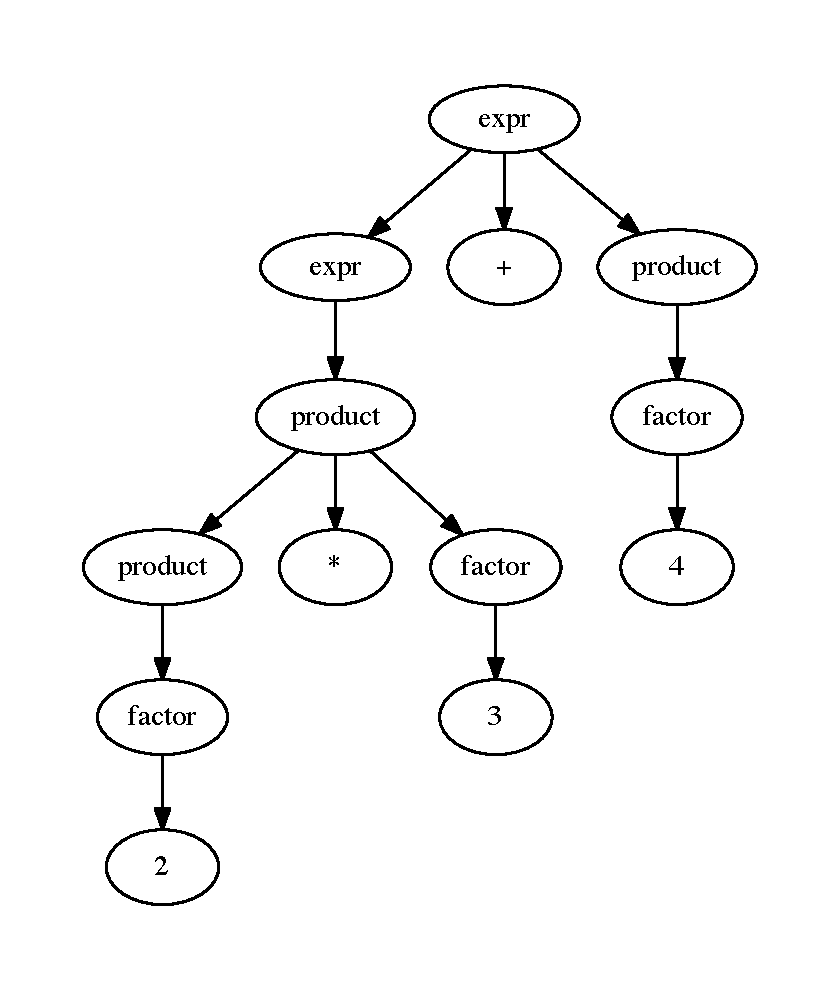
\epsfig{file=Abbildungen/parse-tree.eps, scale=0.6}
  \caption{Ein Parse-Baum f\"ur den String ``\texttt{2*3+4}''.}
  \label{fig:parse-tree.dot2}
\end{figure}

Fassen wir diesen Parse-Baum als Liste seiner
Zweige auf, wobei jeder Zweig eine Liste von Grammatik-Symbolen ist, so erhalten wir die folgende Liste:
\\[0.2cm]
\hspace*{1.3cm}
$
\begin{array}[b]{rl}
  \bigl[ 
 & [ \textsl{expr}, \textsl{expr}, \textsl{product}, \textsl{product}, \textsl{factor}, \quoted{2} ],
   \\[0.1cm] 
 & [ \textsl{expr}, \textsl{expr}, \textsl{product}, \quoted{*} ],
   \\[0.1cm] 
 & [ \textsl{expr}, \textsl{expr}, \textsl{product}, \textsl{factor}, \quoted{3} ],
   \\[0.1cm] 
 & [ \textsl{expr}, \quoted{+} ],
   \\[0.1cm] 
 & [ \textsl{expr}, \textsl{product}, \textsl{factor}, \quoted{4} ]
   \\[0.1cm] 
  \bigr]. 
\end{array}
$ \eox
\pagebreak

\noindent
Die nun folgende Definition der Funktion $\textsl{parseTree}()$ formalisiert die
Berechnung des Parse-Baums.

\begin{Definition}[\textsl{parseTree}] \lb
Ist $G = \langle V, T, R, S \rangle$ eine kontextfreie Grammatik, ist $w \in T^*$, $A \in V$ und  gibt es eine Ableitung
\[ A \Rightarrow^* w,  \]
so definieren wir $\textsl{parseTree}(A \Rightarrow^* w)$ induktiv als Liste von Listen:
\begin{enumerate}
\item Falls $(A \rightarrow t_1t_2 \cdots t_m)\in R$ mit $A \in V$ und $t_1 \cdots t_m = w$ ist,
      so setzen wir
      \\[0.2cm]
      \hspace*{1.3cm}
      $\textsl{parseTree}(A \Rightarrow^* w) = \bigl[\, [A, t_1],\,  [A, t_2],\,\cdots,\,  [A, t_m]\, \bigr]$.  
\item Falls $(A \rightarrow \varepsilon)\in R$ mit $A \in V$ und $w = \varepsilon$ ist, so setzen wir
      \\[0.2cm]
      \hspace*{1.3cm}
      $\textsl{parseTree}(A \Rightarrow^* w) = \bigl[\, [A, \varepsilon]\, \bigr]$.  
\item Falls  $A \Rightarrow^* w$ gilt, weil
      \\[0.2cm]
      \hspace*{1.3cm}
      $ (A \rightarrow B_1B_2 \cdots B_m) \in R, \quad 
         B_i \Rightarrow^* w_i\; \mbox{f\"ur alle $i=1,\cdots,m$} \quad
         \mbox{und} \; w = w_1w_2 \cdots w_m
      $
      \\[0.2cm]
      gilt, so definieren wir (unter Benutzung der \textsc{SetlX}-Notation f\"ur die Definition von Listen)
      \\[0.2cm]
      \hspace*{1.3cm}
      $ 
        \textsl{parseTree}(A \Rightarrow^*w)  =
        \bigl[\; [A] + l \,:\,
                 i \in [1, \cdots, m ],\, l \in \textsl{parseTree}(B_i \Rightarrow^* w_i) \;
        \bigr]
      $.
      \\[0.2cm]
      Damit diese Definition auch tats\"achlich alle F\"alle abdeckt, m\"ussen wir noch den Fall
      diskutieren, dass  eines der Symbole $B_i$ ein Terminal ist: In diesem Fall setzen wir
      \\[0.2cm]
      \hspace*{1.3cm}
      $\textsl{parseTree}(B_i \Rightarrow^* B_i) := \bigl[ [B_i] \bigr]$.
\end{enumerate}
\end{Definition}

Wir definieren die \emph{Breite} $b$ einer Grammatik als die gr\"o{\ss}te Anzahl von Symbolen, die 
auf der rechten Seite einer Grammatik-Regel der Form
\\[0.2cm]
\hspace*{1.3cm}
$A \rightarrow \alpha$
\\[0.2cm]
auftreten.  

\begin{Lemma}[Beschr\"anktheits-Lemma] \label{lemma:length}
  Die Grammatik $G = \langle V, T, R, S \rangle$ habe die Breite $b$.  Ferner gelte
  \\[0.2cm]
  \hspace*{1.3cm}
  $A \Rightarrow^* w$
  \\[0.2cm]
  f\"ur eine syntaktische Variable $A \in V$ und ein Wort $w \in T^*$.  Falls $n$ die L\"ange der l\"angsten Liste in
  \[ \textsl{parseTree}(A \Rightarrow^* w) \]
  ist, so gilt f\"ur die L\"ange des Wortes $w$ die Absch\"atzung
  \\[0.2cm]
  \hspace*{1.3cm}
  $|w| \leq b^{n-1}$.  
\end{Lemma}

\noindent
\textbf{Beweis}: Wir f\"uhren den Beweis durch Induktion nach der L\"ange $n$ der l\"angsten
Liste in $\textsl{parseTree}(A \Rightarrow^* w)$.
\begin{enumerate}
\item[I.A.] $n=2$:  Wenn alle Listen in $\textsl{parseTree}(A \Rightarrow^* w)$ 
            nur zwei Elemente haben, dann besteht die Ableitung aus genau einem Schritt
            und daher muss es eine Regel der Form 
            \\[0.2cm]
            \hspace*{1.3cm}
            $A \rightarrow t_1t_2 \cdots t_m$ \quad mit $w = t_1t_2 \cdots t_m$ und $t_i \in T$
            f\"ur alle $i=1,\cdots,m$
            \\[0.2cm]
            in der Grammatik $G$ geben.  Es gilt dann
            \[ \textsl{parseTree}(A \Rightarrow^* w) = 
               \bigl[\, [A,t_1],\, [A,t_2],\, \cdots,\; [A,t_m]\, \bigr].\, 
            \]
            Daraus folgt
            \\[0.2cm]
            \hspace*{1.3cm}
            $|w| = |t_1t_2 \cdots t_m| = m \leq b = b^{1} = b^{2-1}$,
            \\[0.2cm]
            wobei die Ungleichung $m \leq b$ aus der Tatsache folgt, dass die L\"ange der Regeln der Grammatik
            $G$ durch die Breite $b$ beschr\"ankt ist.
\item[I.S.] $n \mapsto n+1$: Da die Ableitung nun aus mehr als einem Schritt besteht, hat die Ableitung die Form
            \\[0.2cm]
            \hspace*{1.3cm}
            $A \Rightarrow B_1 B_2 \cdots B_m \Rightarrow^* w_1 w_2 \cdots w_m = w$.
            \\[0.2cm]
            Au{\ss}erdem haben dann die Listen in
            \[ 
               \textsl{parseTree}(B_i \Rightarrow^* w_i) 
            \]
            f\"ur alle $i=1,\cdots,m$ h\"ochstens die L\"ange $n$.
            Nach Induktions-Voraussetzung wissen wir also, dass
            \\[0.2cm]
            \hspace*{1.3cm}
            $|w_i| \leq b^{n-1}$ \quad f\"ur alle $i=1,\cdots,m$
            \\[0.2cm]
            gilt.  Daher haben wir
            \\[0.2cm]
            \hspace*{1.3cm}
            $|w| = |w_1| + \cdots + |w_m| \leq b^{n-1} + \cdots + b^{n-1} = 
             m \cdot b^{n-1} \leq b \cdot b^{n-1} = b^{n} = b^{(n+1)-1}
            $. \qed
\end{enumerate}

\section{Das Pumping-Lemma f\"ur kontextfreie Sprachen}
\begin{Satz}[Pumping-Lemma]
Es sei $L$ eine kontextfreie Sprache.  Dann gibt es ein $n \in \mathbb{N}$, so dass jeder String
$s \in L$, dessen L\"ange gr\"o{\ss}er oder gleich $n$ ist, in der Form 
\[ s = uvwxy \]
geschrieben werden kann, so dass au{\ss}erdem folgendes gilt:
\begin{enumerate}
\item $|vwx| \leq n$,

      der mittlere Teil des Strings hat folglich eine L\"ange von h\"ochstens $n$ Buchstaben.
\item $vx \not= \varepsilon$,

      die Teilstrings $v$ und $x$ k\"onnen also nicht beide gleichzeitig leer sein.
\item $\forall h \in \mathbb{N}: uv^hwx^hy \in L$.

      die Strings $v$ und $x$ k\"onnen beliebig oft repliziert (\emph{gepumpt}) werden. 
\end{enumerate}
\end{Satz}

\noindent
\textbf{Beweis}:  Da $L$ eine kontextfreie Sprache ist, gibt es eine kontextfreie
Grammatik $G = \langle V, T, R, S \rangle$, so dass 
\[ L = L(G) \]
gilt. Wir nehmen an, dass die Grammatik $G$ insgesamt $k$ syntaktische Variablen enth\"alt
und au{\ss}erdem die 
Breite $b$ hat.  Wir definieren
\\[0.2cm]
\hspace*{1.3cm}
$n := b^{k+1}$. 
\\[0.2cm] 
Sei nun $s \in L$ mit $|s| \geq n$.  Wir w\"ahlen einen Parse-Baum $\tau$ aus, der einerseits
den String $s$ ableitet und der andererseits unter allen Parse-B\"aumen, die den String $s$
aus $S$ ableiten, die minimale Anzahl von Knoten hat.  F\"ur diesen Parse-Baum $\tau$
betrachten wir die Listen aus
\\[0.2cm]
\hspace*{1.3cm}
$\tau = \textsl{parseTree}(S \Rightarrow^* s)$. 
\\[0.2cm] 
Falls alle Listen hier eine L\"ange kleiner-gleich $k+1$ h\"atten, so w\"urde aus den Beschr\"anktheits-Lemma
\ref{lemma:length} folgen, dass  
\\[0.2cm]
\hspace*{1.3cm}
$ |s| \leq b^{(k+1)-1} = b^k < b^{k+1} = n, \quad \mbox{also} \quad |s| < n$
\\[0.2cm] 
gilt, im Widerspruch zu der Voraussetzung $|s| \geq n$.  Also muss es in 
$\tau$ eine Liste geben, die mindestens die L\"ange $k + 2$
hat.  Wir w\"ahlen die l\"angste Liste unter den  Listen in $\tau$ aus.
Diese Liste hat dann die Form
\[ [A_1, \cdots, A_l, t] \quad \mbox{mit $A_i \in V$ f\"ur alle $i \in \{1,\cdots,l\}$},\quad t \in T,
   \quad \mbox{sowie $l \geq k+1$}.
 \]
Wegen $l \geq k + 1$  k\"onnen nicht alle Variablen $A_1$, $\cdots$, $A_l$
voneinander verschieden sein, denn es gibt ja nur insgesamt $k$ verschiedene syntaktische
Variablen.   Wir finden daher in der Menge $\{ l, l-1, \cdots, l-k \}$
zwei verschiedene Indizes $i$ und $j$,  so dass die Variablen $A_i$ und $A_j$ gleich sind und definieren
$A := A_i = A_j$.  Von den beiden Indizes $i$ und $j$ bezeichne $i$ den kleineren Index,
es gelte also $i < j$.   Die Ableitung von $s$ aus $S$ hat dann die folgende Form
\[ S \Rightarrow^* u A_i y \Rightarrow^* u v A_j x y \Rightarrow^* u v w x y = s. \] 
Insbesondere gilt also
\[ S \Rightarrow^* u A y, \quad A \Rightarrow^* vAx, \quad \mbox{und} \quad A \Rightarrow^* w. \]
Damit haben wir aber folgendes:
\begin{enumerate}
\item $S \Rightarrow^* uAy \Rightarrow^* uwy$, also
      \[ S \Rightarrow^* uv^0wx^0y. \]
\item $S \Rightarrow^* uAy \Rightarrow^* uvAxy \Rightarrow^* uvvAxxy \Rightarrow^* uvvwxxy$, also
      \[ S \Rightarrow^* uv^2wx^2y. \]
\item $S \Rightarrow^* uAy \Rightarrow^* uvAxy \Rightarrow^* uv^2Ax^2y \Rightarrow^* uv^3Ax^3y
       \Rightarrow^* \cdots \Rightarrow^* uv^hAx^hy \Rightarrow^* uv^hwx^hy$, also
      \\[0.2cm]
      \hspace*{1.3cm}
      $uv^hwx^hy \in L$ \quad f\"ur beliebige $h \in \mathbb{N}$.
      \vspace*{0.2cm}

\end{enumerate}
Wir m\"ussen jetzt noch zeigen, dass $vx \not= \varepsilon$ gilt.  Die Ableitung
\[ A \Rightarrow^* vAx \]
ist eigentlich die Ableitung
\[ A_i \Rightarrow^* vA_jx \]
und enth\"alt daher mindestens einen Ableitungsschritt.
Wir f\"uhren den Nachweis der Behauptung $vx \not= \varepsilon$ indirekt und nehmen $v = x =
\varepsilon$ an.
Dann w\"urde wegen $A_i = A_j$ also
\\[0.2cm]
\hspace*{1.3cm}
$A_i \Rightarrow^+ A_i$
\\[0.2cm]
gelten, wobei das Zeichen $^+$ an dem Pfeil $\Rightarrow$ anzeigt, dass diese Ableitung
mindestens einen Schritt 
enth\"alt.  In diesem Fall w\"are aber der Parse-Baum $\tau$ nicht minimal, denn wir k\"onnten
die Ableitungs-Schritte, die $A_i$ in $A_i$ \"uberf\"uhren, einfach weglassen.
Damit ist die Annahme $vx = \varepsilon$ widerlegt und es muss $vx \not= \varepsilon$ gelten.
\vspace*{0.2cm}

Als letztes zeigen wir, dass die Ungleichung $|vwx| \leq n$ gilt.  Wir haben
\[ A = A_i \Rightarrow^* vA_jx \Rightarrow^* vwx. \]
Weil einerseits $i \in \{l-k, l-(k-1), \cdots,l \}$ gilt und andererseits die der
Ableitung
$A \Rightarrow^* vwx$ zugeordnete Liste aus $\textsl{parseTree}(S \Rightarrow^* w)$ von
maximaler L\"ange war, wissen wir, 
dass die L\"ange der l\"angsten Liste in 
\[ \textsl{parseTree}(A \Rightarrow^* vwx) \]
kleiner-gleich  $k+2$ ist.
  Nach dem Beschr\"anktheits-Lemma
\ref{lemma:length} folgt damit f\"ur die L\"ange von $vwx$ die Absch\"atzung
\\[0.2cm]
\hspace*{1.3cm}
$|vwx| \leq b^{(k+2)-1} = b^{k+1} = n$.   \qed


\remark
Das Pumping-Lemma wird in der deutschsprachigen Literatur gelegentlich  als 
``\emph{Schleifensatz}'' bezeichnet.   Es wurde 1961 von Bar-Hillel, Perles und Shamir
\cite{barhillel:1961} bewiesen.

\section{Anwendungen des Pumping-Lemmas}
Wir zeigen, wie mit Hilfe des Pumping-Lemmas der Nachweis erbracht werden kann, dass
bestimmte Sprachen nicht kontextfrei sind.

\subsection{Die Sprache $L = \{ \mathtt{a}^k \mathtt{b}^k \mathtt{c}^k \mid k \in \mathbb{N} \}$ ist
nicht kontextfrei}
Wir weisen nun nach, dass die Sprache
\[ L = \{ \mathtt{a}^k \mathtt{b}^k \mathtt{c}^k \mid k \in \mathbb{N} \} \]
nicht kontextfrei ist.  Wir f\"uhren diesen Nachweis indirekt und nehmen zun\"achst an, dass $L$
kontextfrei ist.  Nach dem Pumping-Lemma gibt es dann eine nat\"urliche Zahl $n$, so dass jeder String
$s \in L$, dessen L\"ange gr\"o{\ss}er oder gleich $n$ ist, sich in Teilstrings der Form
\[ s = uvwxy \]
zerlegen l\"asst, so dass au{\ss}erdem folgendes gilt:
\begin{enumerate}
\item $|vwx| \leq n$,
\item $vx \not= \varepsilon$,
\item $\forall i \in \mathbb{N}: uv^iwx^iy \in L$.

      Insbesondere k\"onnen wir hier $i=0$ w\"ahlen und erhalten dann
      $uwy \in L$. 
\end{enumerate}
Wir definieren nun den String $s$ wie folgt:
\[ s := \mathtt{a}^n\mathtt{b}^n\mathtt{c}^n. \]
Dieser String hat die L\"ange $3 \cdot n \geq n$ und erf\"ullt also die Voraussetzung \"uber die L\"ange.
Damit finden wir eine Zerlegung $s=uvwxy$ mit den obigen Eigenschaften.  Da der Teilstring
$vwx$ eine L\"ange kleiner oder gleich $n$ hat, k\"onnen in diesem String nicht gleichzeitig die
Buchstaben \qote{a} und \qote{c} vorkommen. Wir betrachten die nach dieser Erkenntnis noch
m\"oglichen  F\"alle getrennt.
\begin{enumerate}
\item Fall: In dem String $vwx$ kommen nur die Buchstaben \qote{a} und \qote{b} vor,  der Buchstabe
      \qote{c} kommt nicht vor: 
      \\[0.2cm]
      \hspace*{1.3cm}
      $\textsl{count}(vwx,\mathtt{c}) = 0$.
      \\[0.2cm]
      Da $vx \not= \varepsilon$ ist, folgt
      \\[0.2cm]
      \hspace*{1.3cm}
      $\textsl{count}(vx,\mathtt{a}) + \textsl{count}(vx,\mathtt{b}) > 0$.
      \\[0.2cm]
      Wir nehmen zun\"achst an, dass $\textsl{count}(vx,\mathtt{a}) > 0$ gilt,
      der Fall $\textsl{count}(vx,\mathtt{b}) > 0$ ist analog zu behandeln.
      Dann erhalten wir einerseits
      \[ 
      \begin{array}[t]{lcl}
        \textsl{count}(uwy,\mathtt{c}) & = & \textsl{count}(s,\mathtt{c}) - \textsl{count}(vx,\mathtt{c}) \\
                              & = & \textsl{count}(s,\mathtt{c}) - 0 \\
                              & = & \textsl{count}(\mathtt{a}^n\mathtt{b}^n\mathtt{c}^n,\mathtt{c}) \\
                              & = & n.
      \end{array}
      \]
      Z\"ahlen wir nun die H\"aufigkeit, mit welcher der Buchstabe \qote{a}
      in dem String $uwy$ auftritt, so erhalten wir
      \[ 
      \begin{array}[t]{lcl}
        \textsl{count}(uwy,\mathtt{a}) & = & 
        \textsl{count}(s,\mathtt{a})  - \textsl{count}(vx,\mathtt{a}) \\
                              & < & \textsl{count}(s,\mathtt{a}) \\
                              & = & \textsl{count}(\mathtt{a}^n\mathtt{b}^n\mathtt{c}^n,\mathtt{a}) \\
                              & = & n.
      \end{array}
      \]
      Damit haben wir dann aber
      \\[0.2cm]
      \hspace*{1.3cm}
      $\textsl{count}(uwy,\mathtt{a}) < \textsl{count}(uwy,\mathtt{c})$
      \\[0.2cm]
      und daraus folgt $uwy \not\in L$, was im Widerspruch zum Pumping-Lemma steht.
\item Fall: In dem String $vwx$ kommt der Buchstabe \qote{a} nicht vor.
   
      Dieser Fall l\"asst sich analog zum ersten Fall behandeln. \qed
\end{enumerate}

\exercise
Zeigen Sie, dass die Sprache 
\[ L = \bigl\{ \,\mathtt{a}^{k^2} \;\big|\; k \in \mathbb{N}\, \bigr\} \]
nicht kontextfrei ist. 
\vspace*{0.2cm}

\noindent
\textbf{Hinweis}: Argumentieren Sie \"uber die L\"ange der betrachteten Strings. \eox
\vspace*{0.2cm}

\solution
Wir f\"uhren den Beweis indirekt und nehmen an, dass die Sprache $L_{\mathrm{square}}$ kontextfrei
w\"are.  Nach dem Pumping-Lemma f\"ur kontextfreie Sprachen gibt es dann eine positive
nat\"urliche Zahl $n$, so dass sich jeder String $s \in L_{\mathrm{square}}$ mit $|s| \geq n$ in f\"unf 
Teilstrings $u$, $v$, $w$, $x$, und $y$ aufspalten l\"asst, so dass gilt:
\begin{enumerate}
\item $s = uvwxy$,
\item $|vwx| \leq n$,
\item $vx \not= \varepsilon$,
\item $\forall h \in \mathbb{N}: uv^hwx^hy \in L_{\mathrm{square}}$. 
\end{enumerate} 
Wir betrachten nun den String $s = a^{n^2}$.  F\"ur die L\"ange dieses Strings gilt offenbar
\[ |s| = \big| a^{n^2} \big| = n^2 \geq n. \]
Also gibt es eine Aufspaltung von $s$ der Form $s = uvwxy$ mit den oben angegebenen Eigenschaften.
Da $a$ der einzige Buchstabe ist, der in $s$ vorkommt, k\"onnen in den Teilstrings $u$, $v$, $w$, $x$ und $y$
auch keine anderen Buchstaben vorkommen und es muss nat\"urliche Zahlen $c$, $d$, $e$, $f$, und $g$ geben, so
dass  
\[ u = a^c,\; v = a^d,\; w = a^e,\; x = a^f\; \mbox{und}\; y = a^g \]
gilt.  Wir untersuchen, welche Konzequenzen sich daraus f\"ur die Zahlen $c$, $d$, $e$, $f$, $g$ ergeben.
\begin{enumerate}
\item Die Zerlegung $s = uvwxy$ schreibt sich als $a^{n^2} = a^ca^da^ea^fa^g$ und daraus folgt
      \begin{equation}
        \label{eq:f1}
         n^2 = c + d + e + f + g.     
      \end{equation}
\item Aus der Ungleichung $|vwx| \leq n$ folgt  
      \begin{equation}
        \label{eq:f2}
        d + e + f \leq n.
      \end{equation}
\item Die Bedingung $vx \not= \varepsilon$ liefert
      \begin{equation}
        \label{eq:f3}
        d + f > 0.
      \end{equation}
\item Aus der Formel $\forall h \in \mathbb{N}: uv^hwx^hy \in L_{\mathrm{square}}$ folgt
      \begin{equation}
        \label{eq:f4}
        \forall h \in \mathbb{N}: a^ca^{d\cdot h}a^ea^{f\cdot h}a^g \in L_{\mathrm{square}}. 
      \end{equation}
\end{enumerate}
Die letzte Gleichung muss insbesondere auch f\"ur den Wert $h=2$ gelten:
\[ a^ca^{2\cdot d}a^ea^{2\cdot f}a^g \in L_{\mathrm{square}}.  \]
Nach Definition der Sprache $L_{\mathrm{square}}$ gibt es dann eine nat\"urliche Zahl
$k$, so dass gilt
\begin{equation}
  \label{eq:f5}
  c + 2\cdot d + e + 2\cdot f + g = k^2.
\end{equation}
Addieren wir in Gleichung (\ref{eq:f1}) auf beiden Seiten $d+f$, so erhalten wir insgesamt
\[ n^2 + d + f = c + 2\cdot d + e + 2\cdot f + g = k^2. \]
Wegen $d + f > 0$ folgt daraus 
\begin{equation}
  \label{eq:f6}
  n < k.    
\end{equation}
Andererseits haben wir
\[ 
\begin{array}[t]{lcll}
 k^2  & =    & c + 2\cdot d + e + 2\cdot f + g   & \mbox{nach Gleichung (\ref{eq:f5}})   \\
      & =    & (c + d + e + f + g) + (d + f)     & \mbox{elementare Umformung}           \\
      & \leq & (c + d + e + f + g) + (d + e + f) & \mbox{denn $e \geq 0$}                \\
      & \leq & (c + d + e + f + g) + n           & \mbox{nach Ungleichung (\ref{eq:f2}}) \\
      & =    & n^2 + n                           & \mbox{nach Gleichung (\ref{eq:f1}})   \\
      & <    & n^2 + 2 \cdot n + 1               & \mbox{da $n+1 > 0$}                   \\ 
      & =    & (n+1)^2                           & \mbox{elementare Umformung}           \\ 
\end{array}
\]
Damit haben wir insgesamt  $k^2 < (n+1)^2$ gezeigt und das impliziert
\begin{equation}
  \label{eq:f7}
  k < n+1.
\end{equation}
Zusammen mit Ungleichung (\ref{eq:f6}) liefert Ungleichung (\ref{eq:f7}) nun die Ungleichungs-Kette
\[ n < k < n + 1. \]
Da andererseits $k$ eine nat\"urliche Zahl sein muss und $n$ ebenfalls eine nat\"urliche Zahl ist,
haben wir jetzt einen Widerspruch, denn zwischen $n$ und $n+1$ gibt es keine nat\"urliche Zahl.
\qed


\exercise
Das Alphabet $\Sigma$ sei durch die Festlegung $\Sigma := \{ \mathtt{a}, \mathtt{b} \}$
definiert.  Zeigen Sie, dass die Sprache 
\[ L = \bigl\{ \, tt \;\big|\; t \in \Sigma^*\, \bigr\} \]
nicht kontextfrei ist. \eox

\solution
Wir f\"uhren den Beweis indirekt und nehmen an, dass die Sprache $L$ kontextfrei
w\"are.  Nach dem Pumping-Lemma f\"ur kontextfreie Sprachen gibt es dann eine positive
nat\"urliche Zahl $n$, so dass sich jeder String $s \in L$ mit $|s| \geq n$ in f\"unf 
Teilstrings $u$, $v$, $w$, $x$, und $y$ aufspalten l\"asst, so dass gilt:
\begin{enumerate}
\item $s = uvwxy$,
\item $|vwx| \leq n$,
\item $vx \not= \varepsilon$,
\item $\forall h \in \mathbb{N}: uv^hwx^hy \in L$. 
\end{enumerate} 
Wir betrachten nun den String $s := a^{n}b^{n}a^{n}b^{n}$.  Definieren wir $t:= a^nb^n$,
so ist klar, dass $s = tt$ ist und damit gilt $s \in L$.
F\"ur die L\"ange von $s$ gilt 
\[ |s| = \big| a^{n}b^{n}a^{n}b^{n} \big| = 4 \cdot n \geq n. \]
Also gibt es nach dem Pumping-Lemma eine Aufspaltung von $s$ der Form $s = uvwxy$ mit den
oben angegebenen Eigenschaften. 
Im weiteren f\"uhren wir eine Fallunterscheidung nach der Lage des Strings $vwx$ innerhalb
des gesamten Strings $s = a^{n}b^{n}a^{n}b^{n}$ durch.  Dabei ber\"ucksichtigen wir, dass
$|vwx| \leq n$ gilt.  Zur Vereinfachung der Darstellung des Beweises vereinbaren wir f\"ur zwei Strings
$r$ und $s$ die Schreibweise 
\\[0.2cm]
\hspace*{1.3cm}
$r \sqsubseteq s$ \quad g.d.w. \quad $r$ ist Teilstring von $s$.
\\[0.2cm]
Wollen wir zus\"atzlich die Position einschr\"anken, an der $r$ innerhalb von $s$ auftritt, so
schreiben wir
\\[0.2cm]
\hspace*{1.3cm}
$r \sqsubseteq_{i,j} s$ \quad g.d.w. \quad
$r \sqsubseteq s[i \mathtt{..} j]$. 
\\[0.2cm]
Die Schreibweise $r \sqsubseteq_{i,j} s$ dr\"uckt also aus, dass der Teilstring $r$ ab der
Position $i$ in dem String $s$ auftritt und dass das Ende $r$ nicht \"uber die Position $j$ hinausreicht.


F\"ur die Lage des Teilstrings $vwx$ innerhalb von $a^{n}b^{n}a^{n}b^{n}$ gibt es aufgrund
der L\"angenbeschr\"ankung $|vwx| \leq n$ nur drei M\"oglichkeiten:
\begin{enumerate}
\item Fall: \quad $vwx \sqsubseteq_{1,2\cdot n} a^{n}b^{n}a^{n}b^{n}$,  

      der Teilstring
      $vwx$ liegt also in der ersten H\"alfte von $s$ und ist folglich Teil von
      $a^{n}b^{n}$.
\item Fall: \quad $vwx \sqsubseteq_{n+1,3\cdot n} a^{n}b^{n}a^{n}b^{n}$,  

      der Teilstring
      $vwx$ liegt in der Mitte von $s$ und ist Teil von $b^{n}a^{n}$.
\item Fall: \quad $vwx \sqsubseteq_{2\cdot n+1, 4 \cdot n} a^{n}b^{n}a^{n}b^{n}$,  
  
      der Teilstring
      $vwx$ liegt in der zweiten H\"alfte von $s$ und ist folglich Teil von
      $a^{n}b^{n}$.
\end{enumerate}
Wir setzen nun im Pumping-Lemma in der vierten Aussage f\"ur $h$ den Wert $0$ ein und folgern, dass der
String 
\\[0.2cm]
\hspace*{1.3cm}
$uv^0wx^0y = uwy$ 
\\[0.2cm]
in der Sprache $L$ liegt.  Wir zeigen, dass dies zu einem Widerspruch
f\"uhrt und untersuchen dazu die obigen drei F\"alle der Reihe nach.
\begin{enumerate}
\item Fall: \quad $vwx \sqsubseteq_{1,2\cdot n} a^{n}b^{n}a^{n}b^{n}$.

      Da $vx$ in der ersten H\"alfte von
      $s = a^{n}b^{n}a^{n}b^{n}$ liegt und der String $uwy$ aus $s$ dadurch entsteht, dass
      wir $v$ und $x$ weglassen, hat der String $uwy$ die Form
      \\[0.2cm]
      \hspace*{1.3cm}
      $uwy = a^{n-k_1}b^{n-k_2}a^{n}b^{n}$
      \\[0.2cm]
      und wegen $vx \not= \varepsilon$ wissen wir, dass $k_1 + k_2 > 0$ ist.
      Die Mitte des Strings $uwy$ liegt daher innerhalb des Teilstrings $a^nb^n$.
      Wenn wir also 
      \\[0.2cm]
      \hspace*{1.3cm}
      $t't' = a^{n-k_1}b^{n-k_2}a^{n}b^{n}$ \quad f\"ur ein $t' \in \Sigma^*$
      \\[0.2cm]
      h\"atten, so w\"urde das erste Auftreten von $t'$ in den Teilstring $a^{n}$ hineinragen und m\"usste folglich
      mit einem $a$ enden.  Das funktioniert aber nicht, denn
      das zweite Auftreten von $t'$ endet mit einem $b$.  Also kann dieser Fall nicht eintreten.
\item Fall: \quad $vwx \sqsubseteq_{n+1,3\cdot n} a^{n}b^{n}a^{n}b^{n}$,  

      Da $vx$ nun innerhalb von $s = b^{n}a^{n}$ liegt und der String $uwy$ aus $s$ dadurch
      entsteht, dass wir $v$ und $x$ weglassen, hat der String $uwy$ die Form
      \\[0.2cm]
      \hspace*{1.3cm} $uwy = a^{n}b^{n-k_1}a^{n-k_2}b^{n}$
      \\[0.2cm]
      Wenn $uwy \in L$ ist, m\"usste es also ein $t'$ geben mit
      \\[0.2cm]
      \hspace*{1.3cm} $t't' = a^{n}b^{n-k_1}a^{n-k_2}b^{n}$ \quad und $t' \in \Sigma^*$.
      \\[0.2cm]
      Wenn wir uns das erste Auftreten von $t'$ in dieser Gleichung ansehen, stellen wir fest, dass $t'$ mit
      dem String $a^{n}$ beginnt.  Betrachten wir das zweite Auftreten von $t'$      , so sehen wir, dass 
      $t'$ mit dem String $b^{n}$ endet.  Damit hat dann aber $t'$ mindestens die L\"ange $2
  \cdot n$ und $t't' = uwy$ 
      h\"atte mindestens die L\"ange $4 \cdot n$.  Wegen $vx \not= \varepsilon$  ist dies
      nicht m\"oglich und auch dieser Fall kann nicht eintreten.  

\item Fall: \quad $vwx \sqsubseteq_{2\cdot n+1, 4 \cdot n} a^{n}b^{n}a^{n}b^{n}$.
  
      Dieser Fall ist analog zum ersten Fall.
\end{enumerate}
Da wir in jedem Fall einen Widerspruch erhalten haben, k\"onnen wir schlie{\ss}en, dass die Sprache $L$
nicht kontextfrei sein kann.
\qed

\remarkEng
This result  shows that context-free languages are not closed under complementation, since we have
already shown that the complement of $L$, which is the language
\\[0.2cm]
\hspace*{1.3cm}
$\ds L^{\mathrm{c}} = \bigl\{ s \in \Sigma^* \mid \neg(\exists w\in\Sigma^*: s = ww)\bigr\}$,
\\[0.2cm]
is context-free. \eox
\pagebreak

\exercise
Zeigen Sie, dass die Sprache 
\\[0.2cm]
\hspace*{1.3cm}
$L = \bigl\{ \,\mathtt{a}^{p} \;\big|\; p \in \mathbb{P} \bigr\}$
\\[0.2cm]
nicht kontextfrei ist.  Hier bezeichnet $\mathbb{P}$ die Menge der Primzahlen.
\eox

\solution
Wir f\"uhren den Beweis indirekt und nehmen an, $L$ w\"are kontextfrei.  Nach
dem Pumping-Lemma gibt es dann eine Zahl $n$, so dass es f\"ur alle Strings $s \in L$, 
deren L\"ange gr\"o{\ss}er als $n$ ist, eine Zerlegung
\\[0.2cm]
\hspace*{1.3cm}
$s = uvwxy$
\\[0.2cm]
mit den folgenden drei Eigenschaften gibt:
\begin{enumerate}
\item $|vwx| \leq n$ \quad und
\item $vx \not= \varepsilon$, 
\item $\forall h \in \mathbb{N}: u v^h w x^h y \in L$.
\end{enumerate}
Wir w\"ahlen nun eine Primzahl $p$, die gr\"o{\ss}er als $n+1$ ist und setzen $s = \mathtt{a}^p$.
Wir wissen, dass eine solche Primzahl existieren muss, denn 
\href{http://en.wikipedia.org/wiki/Prime_number#Number_of_prime_numbers}{es gibt unendlich viele Primzahlen}. 
Dann gilt $|s| = p > n$ und die Voraussetzung des Pumping-Lemmas ist erf\"ullt.
Wir finden also eine Zerlegung von $\mathtt{a}^p$ der Form
\\[0.2cm]
\hspace*{1.3cm}
$\mathtt{a}^p = uvwxy$ 
\\[0.2cm]
mit den oben angegebenen Eigenschaften.
Aufgrund der Gleichung $s = uvwxy$ k\"onnen die Teilstrings $u$, $v$, $w$, $x$ und $y$ nur aus dem
Buchstaben ``\texttt{a}'' bestehen.  Also gibt es nat\"urliche Zahlen $c$, $d$, $e$, $f$ und
$g$ so dass gilt:
\\[0.2cm]
\hspace*{1.3cm}
$u = \mathtt{a}^c$, \quad $v = \mathtt{a}^d$, \quad $w = \mathtt{a}^e$, \quad 
$x = \mathtt{a}^f$ \quad und \quad $y = \mathtt{a}^g$.
\\[0.2cm]
F\"ur die Zahlen $c$, $d$, $e$, $f$ und $g$ gilt dann Folgendes:
\begin{enumerate}
\item $c + d + e + f + g = p$,
\item $d + f \not= 0$,
\item $d + e + f \leq n$,
\item $\forall h \in \mathbb{N}: c + h \cdot d + e + h \cdot f + g \in \mathbb{P}$.
\end{enumerate}
Setzen wir in der letzten Gleichung f\"ur $h$ den Wert $(c + e + g)$ ein, so erhalten wir
\\[0.2cm]
\hspace*{1.3cm}
$c + (c + e + g) \cdot d + e + (c + e + g) \cdot f + g \in P$.
\\
Wegen
\\
\hspace*{1.3cm}
$c + (c + e + g) \cdot d + e + (c + e + g) \cdot f + g = (c + e + g) \cdot (1 + d + f)$ 
\\[0.2cm]
h\"atten wir dann
\\[0.2cm]
\hspace*{1.3cm}
$(c + e + g) \cdot (1 + d + f) \in \mathbb{P}$.
\\[0.2cm]
Das kann aber nicht sein, denn wegen $d + f > 0$ ist der Faktor $1 + d + f$ gr\"o{\ss}er als $1$
und wegen
\\[0.2cm]
\hspace*{1.3cm}
 $d + e + f \leq n$, \quad $c + d + e + f + g = p$ \quad und \quad $p > n + 1$ 
\\[0.2cm]
wissen wir, dass 
\\[0.2cm]
\hspace*{1.3cm}
$c + e + g \geq  c + g = c + d + e + f + g - (d + e + f) = p - (d + e + f) \geq p - n > 1$ 
\\[0.2cm]
ist, so dass auch der Faktor $(c + e + g)$ ebenfalls gr\"o{\ss}er als $1$ ist.  Damit kann das
Produkt
\\[0.2cm]
\hspace*{1.3cm}
$(c + e + g) \cdot (1 + d + f)$ 
\\[0.2cm]
aber keine Primzahl sein und wir haben einen
Widerspruch zu der Annahme, dass $L$ kontextfrei ist.
\qed


\exercise
Zeigen Sie, dass die Sprache
$\ds L = \bigl\{ \,\mathtt{a}^{2^k} \mid k \in \mathbb{N} \bigr\}$
nicht kontextfrei ist.  \eox

\exercise
Zeigen Sie, dass die Sprache
$\ds L = \bigl\{ \,\mathtt{a}^{k}\mathtt{b}^l\mathtt{c}^{k \cdot l} \mid k, l \in \mathbb{N} \bigr\}$
nicht kontextfrei ist.  \eox

\exercise
Es seien $L_1$ und $L_2$ kontextfreie Sprachen.  Beweisen oder widerlegen Sie, dass dann auch die
Sprache $L_1 \cap L_2$ kontextfrei ist.  \eox


%%% Local Variables: 
%%% mode: latex
%%% TeX-master: "formal-languages"
%%% End: 

\chapter{Earley-Parser}
In diesem Kapitel stellen wir ein effizientes Verfahren vor, mit dem es m\"oglich ist, f\"ur eine
\underline{beliebi}g\underline{e} vorgegebene kontextfreie Grammatik
\\[0.2cm]
\hspace*{1.3cm}
$G = \langle V, \Sigma, R, S \rangle$ \quad und einen vorgegebenen String $s \in \Sigma^*$
\\[0.2cm]
zu entscheiden, ob $s$ ein Element der Sprache $L(G)$ ist, ob also $s \in L(G)$ gilt.
Der Algorithmus, den wir gleich diskutieren werden, wurde 1970 von Jay Earley publiziert
\cite{earley:70}.  Neben dem Algorithmus von Earley gibt es noch den
\blue{Cocke-Younger-Kasami-Algorithmus}, \index{Cocke-Younger-Kasami-Algorithmus} in der Literatur auch als
\blue{\textsc{Cyk}-Algorithmus} bekannt, \index{\textsc{Cyk}-Algorithmus} der unabh\"angig von John Cocke
\cite{cocke:1970}, Daniel H.~Younger \cite{younger:1967} und Tadao Kasami \cite{kasami:1965} entdeckt wurde.
Der \textsc{Cyk}-Algorithmus ist nur anwendbar, wenn
die Grammatik in \blue{Chomsky-Normalform} vorliegt.  Da es sehr aufwendig ist, eine Grammatik in
Chomsky-Normalform zu transformieren, wird der \textsc{Cyk}-Algorithmus in der
Praxis nicht eingesetzt.  
Demgegen\"uber kann der von Earley angegebene Algorithmus auf beliebige kontextfreie Grammatiken
angewendet werden.  Im allgemeinen Fall hat dieser Algorithmus die Komplexit\"at
$\mathcal{O}(n^3)$, aber falls die vorgegebene Grammatik eindeutig ist, dann ist die Komplexit\"at
lediglich $\mathcal{O}(n^2)$.  Geschickte Implementierungen von Earley's Algorithmus
erreichen f\"ur viele praktisch relevante Grammatiken sogar eine lineare Laufzeit.  
Im Gegensatz hat der \textsc{Cyk}-Algorithmus \textbf{immer} die Komplexit\"at $\mathcal{O}(n^3)$.
Earley's Algorithmus hat sowohl f\"ur $LL(k)$-Grammatiken als auch f\"ur $LR(1)$-Grammatiken, die wir in einem
sp\"ateren Kapitel analysieren werden, nur eine lineare Laufzeit.

Dieses Kapitel gliedert sich in die folgenden Abschnitte:
\begin{enumerate}[(a)]
\item Zun\"achst skizzieren wir die Theorie, die Earley's Algorithmus zu Grunde liegt.
\item Danach geben wir eine einfache Implementierung des Algorithmus in \textsl{Python} an.
%\item Anschlie�end beweisen wir die Korrektheit und Vollst\"andigkeit des Algorithmus.
%\item Zum Abschluss des Kapitels untersuchen wir die Komplexit\"at.
\end{enumerate}

\section{Der Algorithmus von Earley}
Der zentrale Begriff des von Earley angegebenen Algorithmus ist der Begriff des \blue{Earley-Objekts},
das wie folgt definiert ist:

\begin{Definition}[Earley-Objekt]
  Gegeben sei eine kontextfreie Grammatik $G = \langle V, \Sigma, R, S \rangle$ und ein String
  $s = x_1x_2 \cdots x_n \in \Sigma^*$ der L\"ange $n$.  Wir bezeichnen ein Paar der Form
  \\[0.2cm]
  \hspace*{1.3cm}
  $\langle A \rightarrow \alpha \bullet \beta, k \rangle$
  \\[0.2cm]
  genau dann als ein \blue{Earley-Objekt},\index{Earley-Objekt} falls folgendes gilt:
  \begin{enumerate}[(a)]
  \item $(A \rightarrow \alpha \beta) \in R$ \quad und
  \item $k \in \{0,1,\cdots,n\}$. \qed
  \end{enumerate}
\end{Definition}

\noindent
\textbf{Erkl\"arung}: 
Ein Earley-Objekt beschreibt einen Zustand, in dem ein Parser sich befinden kann.  
Ein Earley-Parser, der einen String $x_1 \cdots x_n$ parsen soll,
verwaltet $n+1$ Mengen von Earley-Objekten.  Diese Mengen bezeichnen wir mit
\\[0.2cm]
\hspace*{1.3cm}
$Q_0, Q_1, \cdots, Q_n$.
\\[0.2cm]
Die Interpretation von 
\\[0.2cm]
\hspace*{1.3cm}
$\langle A \rightarrow \alpha \bullet \beta, k \rangle \in Q_j$ \quad mit  $j \geq k$
\\[0.2cm]
ist dann wie folgt:
\begin{enumerate}
\item Der Parser versucht, die Regel $A \rightarrow \alpha \beta$ auf den Teilstring 
      $x_{k+1} \cdots x_n$ anzuwenden und am Anfang dieses Teilstrings ein $A$ mit Hilfe
      der Regel $A \rightarrow \alpha \beta$ zu erkennen.
\item In dem Teilstrings $x_{k+1} \cdots x_j$ hat der Parser bereits $\alpha$ erkannt, es gilt also
      \\[0.2cm]
      \hspace*{1.3cm}
      $\alpha \Rightarrow^* x_{k+1} \cdots x_j$.
\item Folglich versucht der Parser, am Anfang des Teilstrings $x_{j+1} \cdots x_n$ ein
      $\beta$ zu erkennen.
\end{enumerate}
Der Algorithmus von Earley verwaltet f\"ur $j=0,1,\cdots,n$  Mengen $Q_j$ von
Earley-Objekten, die den Zustand beschreiben, in dem der Parser ist, wenn der Teilstring
$x_1 \cdots x_j$ verarbeitet ist.  Zu Beginn des Algorithmus wird der Grammatik ein neues Start-Symbol $\widehat{S}$ 
sowie die Regel $\widehat{S} \rightarrow S$ hinzugef\"ugt.  Die Menge $Q_0$ wird definiert als
\\[0.2cm]
\hspace*{1.3cm}
$Q_0 := \bigl\{ \pair(\widehat{S} \rightarrow \bullet S, 0) \bigr\}$,
\\[0.2cm]
denn der Parser soll ja das Start-Symbol $S$ am Anfang des Strings $x_1 \cdots x_n$ erkennen.
Die restlichen Mengen $Q_j$ sind f\"ur $j=1,\cdots,n$ zun\"achst leer.  Die Mengen $Q_j$ werden nun durch die
folgenden drei Operationen so lange wie m\"oglich erweitert: 
\begin{enumerate}
\item \emph{Lese-Operation}

      Falls der Zustand $Q_j$ ein Earley-Objekt der Form 
      $\pair(A \rightarrow \beta \bullet a \gamma, k)$ enth\"alt, wobei $a$ ein
      Terminal ist, so versucht der Parser, die rechte Seite der Regel
      $A \rightarrow \beta a \gamma$ zu erkennen und hat bis zur Position $j$ bereits den Teil $\beta$ erkannt.
      Folgt auf dieses $\beta$ nun, wie in der Regel $A \rightarrow \beta a \gamma$
      vorgesehen, an der Position $j+1$ das Terminal $a$,
      so muss der Parser nach der Position $j+1$ nur noch $\gamma$ erkennen.  Daher wird in diesem Fall das
      Earley-Objekt 
      \\[0.2cm]
      \hspace*{1.3cm}
      $\pair(A \rightarrow \beta a \bullet \gamma, k)$
      \\[0.2cm]
      dem Zustand $Q_{j+1}$ hinzugef\"ugt:
      \\[0.2cm]
      \hspace*{1.3cm}
      $\pair(A \rightarrow \beta \bullet a \gamma, k) \in Q_j \wedge x_{j+1} = a
       \;\Rightarrow\;
       Q_{j+1} := Q_{j+1} \cup \bigl\{ \pair(A \rightarrow \beta a \bullet \gamma, k) \bigr\}$.
\item \emph{Vorhersage-Operation}

      Falls der Zustand $Q_j$ ein Earley-Objekt der Form $\pair(A \rightarrow \beta \bullet C \delta, k)$
      enth\"alt, wobei $C$ eine syntaktische Variable ist, so versucht der Parser im Zustand
      $Q_j$ den Teilstring $C\delta$ zu erkennen.  Dazu muss der Parser an diesem Punkt ein $C$ erkennen.  
      Wir f\"ugen daher f\"ur jede Regel $C \rightarrow \gamma$ der Grammatik das Earley-Objekt 
      $\pair(C \rightarrow \bullet \gamma, j)$ zu der Menge $Q_j$ hinzu:
      \\[0.2cm]
      \hspace*{1.3cm}
      $\pair(A \rightarrow \beta \bullet C \delta, k) \in Q_j 
       \wedge (C \rightarrow \gamma) \in R 
       \;\Rightarrow\;
       Q_j := Q_j \cup\bigl\{ \pair(C \rightarrow \bullet\gamma, j)\bigr\}$.
\item \emph{Vervollst\"andigungs-Operation}

      Falls der Zustand $Q_i$ ein Earley-Objekt der Form $\pair(C \rightarrow \gamma \bullet, j)$
      enth\"alt und weiter der Zustand $Q_j$ ein Earley-Objekt der Form 
      $\pair(A \rightarrow \beta \bullet C \delta,k)$ enth\"alt, dann hat der Parser im Zustand $Q_j$
      versucht, ein $C$ zu parsen und das $C$ ist im Zustand $Q_i$ erkannt worden.  
      Daher f\"ugen wir dem Zustand
      $Q_i$ nun das Earley-Objekt $\pair(A \rightarrow \beta C \bullet \delta,k)$ hinzu:
      \\[0.2cm]
      \hspace*{1.3cm}
      $\pair(C \rightarrow \gamma \bullet, j) \in Q_i \wedge
       \pair(A \rightarrow \beta \bullet C \delta,k) \in Q_j \;\Rightarrow\;
       Q_i := Q_i \cup \bigl\{ \pair(A \rightarrow \beta C \bullet \delta,k) \bigr\}
      $.
\end{enumerate}
Der Algorithmus von Earley, der einen String der Form $s = x_1 \cdots x_n$ parsen will,  funktioniert nun so:
\begin{enumerate}
\item Wir initialisieren die Zust\"ande $Q_i$ wie folgt:
      \\[0.2cm]
      \hspace*{1.3cm}
      $Q_0 := \bigl\{ \pair(\widehat{S} \rightarrow \bullet S, 0) \bigr\}$,
      \\[0.2cm]
      \hspace*{1.3cm}
      $Q_i := \bigl\{ \bigr\}$ \quad f\"ur $i=1,\cdots,n$.
\item Anschlie{\ss}end lassen wir in einer Schleife $i$ von $0$ bis $n$ laufen und f\"uhren die folgenden 
      Schritte durch:
      \begin{enumerate}[(a)]
      \item Wir vergr\"o{\ss}ern $Q_i$ mit der Vervollst\"andigungs-Operation so lange, bis mit dieser Operation
            keine neuen Earley-Objekte mehr gefunden werden k\"onnen.
      \item Anschlie{\ss}end vergr\"o{\ss}ern wir $Q_i$ mit Hilfe der Vorhersage-Operation.  Diese Operation
            wird ebenfalls so lange durchgef\"uhrt, wie neue Earley-Objekte gefunden werden.
      \item Falls $i < n$ ist, wenden wir die Lese-Operation auf $Q_i$ an und initialisierend damit
            $Q_{i+1}$. 
      \end{enumerate}
      Falls die betrachtete Grammatik $G$ auch $\varepsilon$-Regeln enth\"alt, also Regeln der Form
      \\[0.2cm]
      \hspace*{1.3cm}
      $C \rightarrow \varepsilon$,
      \\[0.2cm]
      dann kann es passieren, dass durch die Anwendung einer Vorhersage-Operation eine neue Anwendung
      der Vervollst\"andigungs-Operation m\"oglich wird.  In diesem Fall m\"ussen Vorhersage-Operation und
      Vervollst\"andigungs-Operation so lange iteriert werden, bis durch Anwendung dieser beiden
      Operationen keine neuen Earley-Objekte mehr erzeugt werden k\"onnen.
\item Falls nach Beendigung des Algorithmus die Menge $Q_n$ das Earley-Objekt 
      $\pair(\widehat{S} \rightarrow S \bullet,0)$ enth\"alt, dann war das Parsen erfolgreich und 
      der String $x_1 \cdots x_n$ liegt in der von der Grammatik erzeugten Sprache.
\end{enumerate}
  
\example
Abbildung \ref{fig:expr-small} zeigt eine vereinfachte Grammatik f\"ur arithmetische
Ausdr\"ucke, die nur aus den Zahlen ``1'', ``2'' und ``3'' und den beiden Operator-Symbolen
``\texttt{+}'' und ``\texttt{*}'' aufgebaut ist.  Die Menge $T$ der Terminale dieser
Grammatik ist also durch
\\[0.2cm]
\hspace*{1.3cm}
 $T = \{ \quoted{1}, \quoted{2}, \quoted{3}, \quoted{+}, \quoted{*} \}$
\\[0.2cm]
gegeben.
Wir zeigen, wie sich der String
``\texttt{1+2*3}'' mit dieser Grammatik und dem Algorithmus von Earley parsen l\"asst.
In der folgenden Darstellung werden wir die syntaktische Variable \texttt{expr} mit
dem Buchstaben $E$ abk\"urzen, f\"ur \texttt{prod} schreiben wir $P$ und f\"ur \texttt{fact} verwenden wir die
Abk\"urzung $F$.


\begin{figure}[!ht]
\centering
\begin{Verbatim}[ frame         = lines, 
                  framesep      = 0.3cm, 
                  labelposition = bottomline,
                  numbers       = left,
                  numbersep     = -0.2cm,
                  xleftmargin   = 0.8cm,
                  xrightmargin  = 0.8cm,
                ]
    expr : expr '+' prod
         | prod
         ;
    
    prod : prod '*' fact
         | fact
         ;
    
    fact : '1'
         | '2'
         | '3'
         ;
\end{Verbatim}
\vspace*{-0.3cm}
  \caption{Eine vereinfachte Grammatik f\"ur arithmetische Ausdr\"ucke.}
  \label{fig:expr-small} 
\end{figure}


\begin{enumerate}
\item Wir initialisieren $Q_0$ als
      \\[0.2cm]
      \hspace*{1.3cm}
      $Q_0 = \{ \pair(\widehat{S} \rightarrow \bullet\, E, 0) \}$. 
      \\[0.2cm]
      Die Mengen $Q_1$, $Q_2$, $Q_3$, $Q_4$ und $Q_5$ sind zun\"achst alle leer.
      Wenden wir die Vervollst\"andigungs-Operation auf $Q_0$ an, so finden wir keine neuen
      Earley-Objekte.

      Anschlie{\ss}end wenden wir die Vorhersage-Operation auf das Earley-Objekt 
      $\pair(\widehat{S} \rightarrow \bullet\, E, 0)$ an.  Dadurch werden der Menge $Q_0$ 
      zun\"achst die beiden Earley-Objekte 
      \\[0.2cm]
      \hspace*{1.3cm}
      $\pair(E \rightarrow \bullet\; E \squoted{+} P, 0)$ 
      \quad und \quad
      $\pair(E \rightarrow \bullet\; P, 0)$ 
      \\[0.2cm]
      hinzugef\"ugt.  Auf das Earley-Objekt $\pair(E \rightarrow \bullet\, P, 0)$ 
      k\"onnen wir die Vorhersage-Operation ein weiteres Mal anwenden und erhalten dann die beiden
      neuen Earley-Objekte
      \\[0.2cm]
      \hspace*{1.3cm}
      $\pair(P \rightarrow \bullet\; P \squoted{*} F, 0)$ 
      \quad und\quad 
      $\pair(P \rightarrow \bullet\; F, 0)$. 
      \\[0.2cm]
      Wenden wir auf das Earley-Objekt $\pair(P \rightarrow \bullet\; F, 0)$
      die Vorhersage-Operation an, so erhalten wir schie{\ss}lich noch die folgenden Earley-Objekte in $Q_0$:
      \\[0.2cm]
      \hspace*{1.3cm}
      $\pair(F \rightarrow \bullet \squoted{1}, 0)$, \quad 
      $\pair(F \rightarrow \bullet \squoted{2}, 0)$, \quad und \quad
      $\pair(F \rightarrow \bullet \squoted{3}, 0)$. 
      \\[0.2cm]
      Insgesamt enth\"alt $Q_0$ nun die folgenden Earley-Objekte:
      \begin{enumerate}
      \item $\pair(\widehat{S} \rightarrow \bullet\; E, 0)$,
      \item $\pair(E \rightarrow \bullet\; E \squoted{+} P, 0)$
      \item $\pair(E \rightarrow \bullet\; P, 0)$,
      \item $\pair(P \rightarrow \bullet\; P \squoted{*} F, 0)$,
      \item $\pair(P \rightarrow \bullet\; F, 0)$,
      \item $\pair(F \rightarrow \bullet \squoted{1}, 0)$,
      \item $\pair(F \rightarrow \bullet \squoted{2}, 0)$,
      \item $\pair(F \rightarrow \bullet \squoted{3}, 0)$.
      \end{enumerate}

      Jetzt wenden wir die Lese-Operation auf $Q_0$ an.  Da das erste Zeichen des zu parsenden Strings eine
      ``1'' ist, hat die Menge  $Q_1$ danach die folgende Form:
      \\[0.2cm]
      \hspace*{1.3cm}
      $Q_1 = \bigl\{ \pair(F \rightarrow \squoted{1} \bullet, 0) \bigr\}$.
\item Nun setzen wir $i= 1$ und wenden zun\"achst auf $Q_1$ die Vervollst\"andigungs-Operation an.
      Aufgrund des Earley-Objekts $\pair(F \rightarrow \squoted{1} \bullet, 0) $ in $Q_1$
      suchen wir in $Q_0$ ein Earley-Objekt, bei dem die Markierung ``$\bullet$'' vor der Variablen
      $F$ steht.  Wir finden das Earley-Objekt
      $\pair(P \rightarrow \bullet\; F, 0)$.  Daher f\"ugen wir nun
      $Q_1$ das Earley-Objekt
      \\[0.2cm]
      \hspace*{1.3cm}
      $\pair(P \rightarrow F \;\bullet, 0)$ 
      \\[0.2cm]
      hinzu.  Hierauf k\"onnen wir wieder die
      Vervollst\"andigungs-Operation anwenden und finden (nach mehrmaliger Anwendung) f\"ur $Q_1$ insgesamt die folgenden Earley-Objekte:
      \begin{enumerate}
      \item $\pair(P \rightarrow F \;\bullet, 0)$, 
      \item $\pair(P \rightarrow  P\;\bullet \squoted{*} F, 0)$, 
      \item $\pair(E \rightarrow P \; \bullet, 0)$,
      \item $\pair(E \rightarrow E\;\bullet \squoted{+} P, 0)$,
      \item $\pair(\widehat{S} \rightarrow  E\;\bullet, 0)$.
      \end{enumerate}
      
      Als n\"achstes wenden wir auf diese Earley-Objekte die Vorhersage-Operation an.  Da das
      Markierungs-Zeichen ``$\bullet$'' aber in keinem der in $Q_i$ auftretenden Earley-Objekte vor einer 
      Variablen steht, ergeben sich hierbei keine neuen Earley-Objekte.

      Als letztes wenden wir die Lese-Operation auf $Q_1$ an.  Da in dem String
      ``\texttt{1+2*3}'' das Zeichen ``\texttt{+}'' an der Position 2 liegt ist und $Q_1$ das Earley-Objekt 
      \\[0.2cm]
      \hspace*{1.3cm}
      $\pair(E \rightarrow E\;\bullet \squoted{+} P, 0)$
      \\[0.2cm]
      enth\"alt, f\"ugen wir in $Q_2$  das Earley-Objekt
      \\[0.2cm]
      \hspace*{1.3cm}
      $\pair(E \rightarrow E \squoted{+}\bullet\; P, 0)$
      \\[0.2cm]
      ein.
\item Nun setzen wir $i= 2$ und wenden zun\"achst auf $Q_2$ die Vervollst\"andigungs-Operation
      an.  Zu diesem Zeitpunkt gilt
      \\[0.2cm]
      \hspace*{1.3cm}
      $Q_2 = \{ \pair(E \rightarrow E \squoted{+}\bullet\; P, 0) \}$.
      \\[0.2cm]
      Da in dem einzigen Earley-Objekt, das hier auftritt, das Markierungs-Zeichen ``$\bullet$''
      nicht am Ende der Grammatik-Regel steht, finden wir durch die Vervollst\"andigungs-Operation in
      diesem Schritt keine       neuen Earley-Objekte. 

      Als n\"achstes wenden wir auf $Q_2$ die Vorhersage-Operation an.  Da das Markierungs-Zeichen
      vor der Variablen $P$ steht, finden wir zun\"achst die beiden Earley-Objekte
      \\[0.2cm]
      \hspace*{1.3cm}
      $\pair(P \rightarrow \bullet\; F, 2)$ \quad und \quad
      $\pair(P \rightarrow \bullet\; P \squoted{*} F, 2)$.
      \\[0.2cm]
      Da in dem ersten Earley-Objekt das Markierungs-Zeichen vor der Variablen $F$ steht, kann 
      die Vorhersage-Operation ein weiteres 
      Mal angewendet werden und wir finden noch die folgenden Earley-Objekte:
      \begin{enumerate}
      \item $\pair(F \rightarrow \bullet \squoted{1}, 2)$, 
      \item $\pair(F \rightarrow \bullet \squoted{2}, 2)$,
      \item $\pair(F \rightarrow \bullet \squoted{3}, 2)$.
      \end{enumerate}

      Als letztes wenden wir die Lese-Operation auf $Q_2$ an.  Da das dritte Zeichen in dem zu lesenden
      String ``\texttt{1+2*3}'' die Ziffer ``2'' ist, hat $Q_3$ nun die Form
      \\[0.2cm]
      \hspace*{1.3cm}
      $Q_3 = \{ \pair(F \rightarrow \squoted{2}\bullet, 2) \}$.
\item Wir setzen $i = 3$ und wenden auf $Q_3$ die Vervollst\"andigungs-Operation an.
      Dadurch f\"ugen wir 
      \\[0.2cm]
      \hspace*{1.3cm}
      $\pair(P \rightarrow F \;\bullet, 2)$ 
      \\[0.2cm]
      in $Q_3$ ein.  Hier k\"onnen wir ein weiteres Mal die Vervollst\"andigungs-Operation anwenden. 
      Durch iterierte Anwendung der Vervollst\"andigungs-Operation erhalten wir zus\"atzlich die folgenden 
      Earley-Objekte:
      \begin{enumerate}
      \item $\pair(P \rightarrow P \bullet \squoted{*} F, 2)$,
      \item $\pair(E \rightarrow E \squoted{+} P\;\bullet, 0)$,
      \item $\pair(E \rightarrow E\;\bullet \squoted{+} P, 0)$
      \item $\pair(\widehat{S} \rightarrow E\;\bullet, 0)$.
      \end{enumerate}
      Als letztes wenden wir die Lese-Operation an.  Da der n\"achste zu lesende Buchstabe das Zeichen
      ``\texttt{*}'' ist, erhalten wir
      \\[0.2cm]
      \hspace*{1.3cm}
      $Q_4 = \{ \pair(P \rightarrow P \squoted{*} \bullet\, F, 2) \}$.
\item Wir setzen $i= 4$.  Die Vervollst\"andigungs-Operation liefert keine neuen Earley-Objekte.
      Die Vorhersage-Operation liefert folgende Earley-Objekte:
      \begin{enumerate}
      \item $\pair(F \rightarrow \bullet \squoted{1}, 4)$, 
      \item $\pair(F \rightarrow \bullet \squoted{2}, 4)$,
      \item $\pair(F \rightarrow \bullet \squoted{3}, 4)$.
      \end{enumerate}
      Da das n\"achste Zeichen die Ziffer ``3'' ist, liefert die Lese-Operation f\"ur $Q_5$:
      \\[0.2cm]
      \hspace*{1.3cm}
      $Q_5 = \pair(F \rightarrow \squoted{3}\bullet, 4) \}$.
\item Wir setzen $i=5$.  Die Vervollst\"andigungs-Operation liefert nacheinander die folgenden
      Earley-Objekte:
      \begin{enumerate}
      \item $\pair(P \rightarrow P \squoted{*} F\;\bullet, 2)$,
      \item $\pair(E \rightarrow E \squoted{+} P\;\bullet, 0)$,
      \item $\pair(P \rightarrow  P \;\bullet\squoted{*} F, 2)$,
      \item $\pair(E \rightarrow E \;\bullet\squoted{+} P, 0)$ 
      \item $\pair(\widehat{S} \rightarrow  E\;\bullet, 0)$.
      \end{enumerate}
\end{enumerate}
Da die Menge $Q_5$ das Earley-Objekt $\pair(\widehat{S} \rightarrow  E\;\bullet, 0)$ enth\"alt,
k\"onnen wir schlie{\ss}en, dass der String ``\texttt{1+2*3}'' tats\"achlich in der von der Grammatik erzeugten
Sprache liegt.
\vspace*{0.3cm}

\exercise
Zeigen Sie, dass der String ``\texttt{1*2+3}'' in der Sprache der Grammatik liegt, die in 
Abbildung \ref{fig:expr-small} gezeigt wird.  Benutzen Sie dazu den von Earley
angegebenen Algorithmus.

\section{Implementing Earley's Algorithm in \textsl{Python}}
The \textsl{Jupyter} notebook
\\[0.2cm]
\hspace*{-0.3cm}
\href{https://github.com/karlstroetmann/Formal-Languages/blob/master/ANTLR4-Python/Earley-Parser/Earley-Parser.ipynb}{https://github.com/karlstroetmann/Formal-Languages/blob/master/ANTLR4-Python/Earley-Parser/Earley-Parser.ipynb}
\\[0.2cm]
contains an implementation of Earley's algorithm.

\section{Pr\"ufen Sie Ihr Verst\"andnis}
\begin{enumerate}[(a)]
\item Was ist ein Earley-Objekt und wie werden die Komponenten eines Earley-Objekts interpretiert?
\item Wie funktioniert die Lese-Operation beim Algorithmus von Earley?
\item Wie funktioniert die Vorhersage-Operation beim Algorithmus von Earley?
\item Wie funktioniert die Vervollst\"andigungs-Operation beim Algorithmus von Earley?
\item Skizzieren Sie den Algorithmus von Earley f\"ur den Fall, dass die Grammatik keine $\varepsilon$-Regeln enth\"alt.
\item Welche Komplexit\"at hat der Algorithmus von Earley im allgemeinen Fall?
\item Welche Komplexit\"at hat der Algorithmus von Earley in dem Fall, dass die Grammatik eindeutig ist?
\end{enumerate}


%%% Local Variables: 
%%% mode: latex
%%% TeX-master: "formal-languages"
%%% End: 

\chapter{Bottom-Up-Parser\label{chapter:bottom-up}}
Bei der Konstruktion eines Parsers gibt es generell zwei M�glichkeiten:  Wir k�nnen
\blue{Top-Down} oder \blue{Bottom-Up} vorgehen.  Den Top-Down-Ansatz haben wir bereits
diskutiert.  In diesem Kapitel erl�utern wir nun den Bottom-Up-Ansatz.
Dazu stellen wir im n�chsten Abschnitt das allgemeine Konzept vor, das einem
\blue{Bottom-Up-Parser} zu Grunde liegt.  
Im darauf folgenden Abschnitt zeigen wir, wie Bottom-Up-Parser implementiert werden k�nnen
und stellen als eine Implementierungsm�glichkeit die \blue{Shift-Reduce-Parser} vor.
Ein Shift-Reduce-Parser arbeitet mit Hilfe einer Tabelle, in der
hinterlegt ist, wie der Parser in einem bestimmten Zustand die Eingaben verarbeiten muss.
Die Theorie, wie eine solche Tabelle sinnvoll mit Informationen gef�llt werden kann,
entwickeln wir dann in dem folgenden Abschnitt: Zun�chst diskutieren wir die
\blue{SLR-Parser} (\blue{simple LR-Parser}).  Dies ist die einfachste Klasse von Shift-Reduce-Parsern.
Das Konzept der SLR-Parser ist leider f�r die Praxis nicht m�chtig genug.  Daher verfeinern wir
dieses Konzept und erhalten so die Klasse der
\blue{kanonischen LR-Parser}.  Da die Tabellen f�r LR-Parser in der Praxis
h�ufig gro� werden, vereinfachen wir diese Tabellen etwas und erh�lt dann das Konzept der
\blue{LALR-Parser}, das von der M�chtigkeit zwischen dem Konzept der \blue{SLR-Parser} und dem
Konzept der \blue{LR-Parser} liegt.  In dem folgenden Kapitel werden wir dann den Parser-Generator
\textsc{Ply} diskutieren, der ein LALR-Parser ist.

\section{Bottom-Up-Parser}
Die mit \textsc{Antlr} erstellten Parser sind sogenannte \blue{Top-Down-Parser}: Ausgehend von dem
Start-Symbol der Grammatik wurde versucht, eine gegebene Eingabe durch Anwendung der verschiedenen
Grammatik-Regeln zu parsen.  Die Parser, die wir nun entwickeln werden, sind
\blue{Bottom-Up-Parser}.  Bei einem solchen Parser ist die Idee, dass wir von dem zu parsenden
String ausgehen und dort Terminale anhand der rechten Seiten der Grammatik-Regeln zusammenfassen.  
Wir geben ein Beispiel und versuchen den String ``\texttt{1 + 2 * 3}'' mit der Grammatik, die durch die
Regeln 
\[ 
\begin{array}[t]{rcl}
  E & \rightarrow & E \quoted{+} P \;|\; P  \\[0.1cm]
  P & \rightarrow & P \quoted{*} F \;|\; F  \\[0.1cm]
  F & \rightarrow & \squoted{1} \;|\; \squoted{2} \;|\; \squoted{3} 
\end{array}
\]
gegeben ist,  zu parsen.  Dazu suchen wir in diesem String
Teilstrings, die den rechten Seiten von Grammatikregeln entsprechen, wobei wir den String
von links nach rechts durchsuchen.  Auf diese Art versuchen wir,
einen Parse-Baum r�ckw�rts von unten aufzubauen:
\\[0.2cm]
\hspace*{0.3cm} 
$
\begin{array}[t]{lcll}
\texttt{1 + 2 * 3} & \Leftarrow & F \texttt{ + 2 * 3} 
                                & (\mbox{Regel:\ }  F \rightarrow  \squoted{1}) \\
                   & \Leftarrow & P \texttt{ + 2 * 3} 
                                & (\mbox{Regel:\ } P \rightarrow F) \\
                   & \Leftarrow & E \texttt{ + 2 * 3} 
                                & (\mbox{Regel:\ }  E \rightarrow  P) \\
                   & \Leftarrow & E \texttt{ + } F \texttt{ * 3} 
                                & (\mbox{Regel:\ } F \rightarrow  \squoted{2}) \\
                   & \Leftarrow & E \texttt{ + } P \texttt{ * 3} 
                                & (\mbox{Regel:\ } P \rightarrow F) \\
                   & \Leftarrow & E \texttt{ + } P \texttt{ * } F 
                                & (\mbox{Regel:\ } F \rightarrow \squoted{3}) \\
                   & \Leftarrow & E \texttt{ + } P & (\mbox{Regel:\ } P \rightarrow P \quoted{*} F) \\
                   & \Leftarrow & E                & (\mbox{Regel:\ } E \rightarrow E \quoted{+} P) 
\end{array}
$
\\[0.2cm]
Im ersten Schritt haben wir beispielsweise die Grammatik-Regel $F \rightarrow \squoted{1}$
benutzt, um den String ``\texttt{1}'' durch $F$ zu ersetzen und dabei dann den String 
``F\texttt{ + 2 * 3}'' erhalten.  Im zweiten Schritt haben wir die Regel
$P \rightarrow F$ benutzt, um $F$ durch $P$ zu
ersetzen.  Auf diese Art und Weise haben wir am Ende den urspr�nglichen String 
``\texttt{1 + 2 * 3}'' auf $E$ zur�ck gef�hrt.  Wir k�nnen an dieser Stelle zwei
Beobachtungen machen:
\begin{enumerate}
\item Wir ersetzen bei unserem Vorgehen immer den am weitesten links stehenden Teilstring,
      der ersetzt werden kann, wenn wir den anfangs gegebenen String auf das Start-Symbol
      der Grammatik zur�ck f�hren wollen.
\item Schreiben wir die Ableitung, die wir r�ckw�rts konstruiert haben, noch einmal
      in der richtigen Reihenfolge hin, so erhalten wir:
\\[0.2cm]
\hspace*{1.3cm}
$
\begin{array}[t]{lcl}
E  & \Rightarrow & E \texttt{ + } P \\
   & \Rightarrow & E \texttt{ + } P \texttt{ * } F \\
   & \Rightarrow & E \texttt{ + } P \texttt{ * 3} \\
   & \Rightarrow & E \texttt{ + } F \texttt{ * 3} \\
   & \Rightarrow & E \texttt{ + 2 * 3} \\
   & \Rightarrow & P \texttt{ + 2 * 3} \\
   & \Rightarrow & F \texttt{ + 2 * 3} \\
   & \Rightarrow & \texttt{1 + 2 * 3}
\end{array}
$
\\[0.2cm]
       Wir sehen hier, dass bei dieser Ableitung immer die am weitesten rechts stehende
       syntaktische Variable ersetzt worden ist.  Eine derartige Ableitung wird als
       \blue{Rechts-Ableitung} \index{Rechts-Ableitung} bezeichnet.   

       Im Gegensatz dazu ist es bei den Ableitungen, die ein \blue{Top-Down-Parser}
       erzeugt, genau umgekehrt:  Dort wird immer die am weitesten links stehende
       syntaktische Variable ersetzt.  Die mit einem solchen Parser erzeugten Ableitungen
       hei�en daher \blue{Links-Ableitungen}. \index{Links-Ableitung}
\end{enumerate}
Die obigen beiden Beobachtungen sind der Grund, weshalb die Parser, die wir in diesem
Kapitel diskutieren, als \blue{LR-Parser} bezeichnet werden.  Das \blue{L} steht f�r
\blue{\underline{l}eft to right} und beschreibt die Vorgehensweise, dass der String immer
von links nach rechts durchsucht wird, w�hrend das \blue{R} f�r 
\blue{\underline{r}everse rightmost derivation} steht
und ausdr�ckt, dass solche Parser eine Rechts-Ableitung r�ckw�rts konstruieren.
\vspace*{0.2cm}

\noindent
Bei der Implementierung eines LR-Parsers stellen sich zwei Fragen:
\begin{enumerate}[(a)]
\item Welche Teilstrings ersetzen wir?
\item Welche Regeln verwenden wir dabei?
\end{enumerate}
Die Beantwortung dieser Fragen ist im Allgemeinen nicht trivial.  Zwar gehen wir die Strings immer
von links nach rechts durch, aber damit ist noch nicht unbeding klar, welchen Teilstring wir
ersetzen, denn die potentiell zu ersetzenden Teilstrings k�nnen sich durchaus �berlappen.
Betrachten wir beispielsweise das Zwischenergebnis
\\[0.2cm]
\hspace*{1.3cm}
$E \texttt{ + } P \texttt{ * 3}$,
\\[0.2cm]
das wir oben im f�nften Schritt erhalten haben.
Hier k�nnten wir den Teilstring ``P'' mit Hilfe der Regel
\\[0.2cm]
\hspace*{1.3cm}
$E \rightarrow P$
\\[0.2cm]
durch ``E'' ersetzen.  Dann w�rden wir den String
\\[0.2cm]
\hspace*{1.3cm}
$E \texttt{ + } E \texttt{ * 3}$
\\[0.2cm]
erhalten.  Die einzigen Reduktionen, die wir jetzt noch durchf�hren k�nnen, f�hren �ber die
Zwischenergebnisse $E \texttt{ + } E \texttt{ * }  F$ und $E \texttt{ + } E \texttt{ * } P$
zu dem String
\\[0.2cm]
\hspace*{1.3cm}
$E \texttt{ + } E \texttt{ * }  E$,
\\[0.2cm]
der sich dann  aber mit der oben angegebenen Grammatik nicht mehr reduzieren l�sst.  
Die Antwort auf die obigen Fragen, welchen Teilstring wir ersetzen und welche Regel wir
verwenden, setzt einiges an Theorie voraus, die wir
in den folgenden Abschnitten entwickeln werden.


\section{Shift-Reduce-Parser}
\blue{Shift-reduce parsing} is one way to implement bottom up parsing.
Assume a grammar $G = \langle V, T, R, S \rangle$ is given.  A  \blue{shift-reduce parser}\index{shift-reduce parser}
is defined as a 4-Tuple
\\[0.2cm]
\hspace*{1.3cm}
$P = \langle Q, q_0, \textsl{action}, \textsl{goto} \rangle$
\\[0.2cm]
where
\begin{enumerate}
\item $Q$ is the set of \blue{states} of the shift-reduce parser.  

      At first, states are purely abstract. 
\item $q_0 \in Q$ is the start state.
\item $\textsl{action}$ is a function taking two arguments. The first argument is a state $q \in Q$
      and the second argument is a terminal $t \in T$.  The result of this function is an element from the set
      \\[0.2cm]
      \hspace*{1.3cm}
      $\textsl{Action} :=
       \bigl\{ \pair(\texttt{shift}, q)  \mid q \in Q \bigr\}               \cup 
       \bigl\{ \pair(\texttt{reduce}, r) \mid r \in R \bigr\} \cup 
       \bigl\{ \texttt{accept} \bigr\}                        \cup
       \bigl\{ \texttt{error}  \bigr\}                         $.
      \\[0.2cm]
      Here \texttt{shift}, \texttt{reduce}, \texttt{accept}, and \texttt{error} are strings that serve to
      distinguish the different kinds of result of the function 
      $\textsl{action}$.  Therefore the signature of the function \textsl{action} is given as follows:
      \\[0.2cm]
      \hspace*{1.3cm}
      $\textsl{action}: Q \times T \rightarrow \textsl{Action}$.
\item \textsl{goto} is a function that takes a state $q \in Q$ and a syntactical variable
      $v \in V$ and computes a new state.  Therefore the signature of \textsl{goto} is as follows:
      \\[0.2cm]
      \hspace*{1.3cm}
      $\textsl{goto}: Q \times V \rightarrow Q$.
\end{enumerate}
A shift-reduce parser uses two stacks:
\begin{enumerate}[(a)]
\item \textsl{States} is a stack of states from the set $Q$:
      \\[0.2cm]
      \hspace*{1.3cm}
      $\textsl{States} \in \textsl{Stack}\langle Q \rangle$.
\item \textsl{Symbols} is a stack of grammar symbols, i.e.~this stack contains both terminals and syntactical
      variables:
      \\[0.2cm]
      \hspace*{1.3cm}
      $\textsl{Symbols} \in \textsl{Stack}\langle T \cup V \rangle$.
\end{enumerate}
In order to simplify the exposition of shift-reduce parsing we assume that the set $T$ of terminals contains
the special symbol ``\textsc{Eof}'' (short for \blue{e}nd \blue{o}f \blue{f}ile).
This symbol is assumed to occur at the end of the input string but does not occur elsewhere.

In order to understand how a shift-reduce parser works we introduce the notion of a
\blue{parser configuration}\index{parser configuration}.  A parser configuration is a triple of the form
\\[0.2cm]
\hspace*{1.3cm}
$\langle\textsl{States}, \textsl{Symbols}, \textsl{Tokens} \rangle$
\\[0.2cm]
where \textsl{States} and \textsl{Symbols} are the aforementioned stacks of states and grammar symbols, while
\textsl{Tokens} is the rest of the 
tokens from the input string that have not been processed.  The stack \textsl{States} always starts with the
start state $q_0$ and has a length that is one more than the length of the stack \textsl{Symbols}.
If the input string that is to be parsed has the form
\\[0.2cm]
\hspace*{1.3cm}
$[t_1, \cdots,t_n]$
\\[0.2cm]
and we have already reduced the first part $[t_1, \cdots,t_k]$ of the input string to produce the symbols 
\\[0.2cm]
\hspace*{1.3cm}
$[X_1,\cdots, X_m]$,
\\[0.2cm]
while $[t_{k+1},\cdots,t_n]$ is the part of the input string that still needs to be processed, then we have
\\[0.2cm]
\hspace*{1.3cm}
$\textsl{States} = [q_0,q_1\cdots, q_m]$, \quad $\textsl{Symbols} = [X_1,\cdots, X_m]$,
\quad and \quad $\textsl{Tokens} = [t_{k+1}, \cdots, t_n, \mathtt{EOF}]$,
\\[0.2cm]
and the parser configuration $\langle \textsl{States}, \textsl{Symbols}, \textsl{Tokens} \rangle$ is written as
\\[0.2cm]
\hspace*{1.3cm}
$q_0, q_1, \cdots, q_m \mid X_1, \cdots. X_m \mid t_{k+1}, \cdots, t_n,\, \mathtt{EOF}$.
\\[0.2cm]
Shift-reduce parsing starts out with the configuration
\\[0.2cm]
\hspace*{1.3cm}
$q_0 \mid \;  \mid t_{1}, \cdots, t_n,\, \mathtt{EOF}$.
\\[0.2cm] 
Then, parsing proceeds iteratively.  If the current configuration is
\\[0.2cm]
\hspace*{1.3cm}
$q_0, q_1, \cdots, q_m \mid X_1, \cdots, X_m \mid t_{k+1}, \cdots, t_n, \,\mathtt{EOF}$,
\\[0.2cm]
then there is a case distinction according to the value of $\textsl{action}(q_m, t_{k+1})$.
\begin{enumerate}[(a)]
\item If $\textsl{action}(q_m, t_{k+1}) = \textsl{error}$, then we know that the given string $t_1\cdots,t_n$
      is not generated by the given grammar and parsing is aborted with an error message.
\item If $\textsl{action}(q_m, t_{k+1}) = \textsl{accept}$, then we must have $t_{k+1} = \mathtt{EOF}$
      and we also must have $X_1 \cdots X_m = S$.  In this case, we have reduced the string $t_1\cdots t_m$
      to the start symbol $S$ of the given grammar and parsing finishes with success.
\item If $\textsl{action}(q_m, t_{k+1}) = \langle\textsl{shift}, q \rangle$, then the current configuration
      is changed into the new configuration
      \\[0.2cm]
      \hspace*{1.3cm}
      $q_0, q_1, \cdots, q_m, q \mid X_1, \cdots, X_m, t_{k+1} \mid t_{k+2}, \cdots, t_n, \,\mathtt{EOF}$,
      \\[0.2cm]
      i.e.~the next token $t_{k+1}$ is moved from the unread input to the top of the symbol stack
      and the new state $q$ is pushed onto the stack \textsl{States}.
\item If $\textsl{action}(q_m, t_{k+1}) = \langle\textsl{reduce}, r \rangle$, where $r$ is a grammar rule,
      then the grammar rule $r$ must have the form
      \\[0.2cm]
      \hspace*{1.3cm}
      $A \rightarrow X_{m-k} \cdots X_{m}$,
      \\[0.2cm]
      i.e.~the right hand side of the grammar rule matches the end of the stack \textsl{Symbols}.
      In this case, the symbols stack is reduced with this grammar rule, i.e.~the symbols
      $X_{m-k} \cdots X_m$ are replaced by $A$.  Furthermore, in the stack \textsl{States} the states
      $q_{m-k} \cdots q_m$ are replaced by the state $\textsl{goto}(q_{m-k-1}, A)$.
      Therefore, the configuration changes as follows:
      \\[0.2cm]
      \hspace*{1.3cm}
      $q_0, q_1, \cdots, q_{m-k-1}, \textsl{goto}(q_{m-k-1}, A) \mid X_1, \cdots, X_{m-k-1}, A \mid t_{k+1}, \cdots, t_n, \,\mathtt{EOF}$.
\end{enumerate}





\begin{figure}[!ht]
\centering
\begin{minted}[ frame         = lines, 
                framesep      = 0.3cm, 
                firstnumber   = 1,
                bgcolor       = sepia,
                numbers       = left,
                numbersep     = -0.2cm,
                xleftmargin   = 0.8cm,
                xrightmargin  = 0.8cm,
              ]{python3}
    class ShiftReduceParser():
        def __init__(self, actionTable, gotoTable):
            self.mActionTable = actionTable
            self.mGotoTable   = gotoTable
\end{minted}
\vspace*{-0.3cm}
\caption{Implementation of a shift-reduce parser in \textsl{Python}}
\label{fig:Shif-Reduce-Parser-Pure.ipynb}
\end{figure}

The class \texttt{Shif-Reduce-Parser-Pure} that is shown in Figure \ref{fig:Shif-Reduce-Parser-Pure.ipynb}
on page \pageref{fig:Shif-Reduce-Parser-Pure.ipynb} displays the class \\
\texttt{ShiftReduceParser}, which
maintains two dictionaries.
\begin{enumerate}[(a)]
\item \texttt{mActionTable} stores the function $\textsl{action}: Q \times T \rightarrow \textsl{Action}$.
\item \texttt{mGotoTable} stores the function $\textsl{goto}: Q \times V \rightarrow Q$.
\end{enumerate}

\begin{figure}[!ht]
\centering
\begin{minted}[ frame         = lines, 
                framesep      = 0.3cm, 
                firstnumber   = 1,
                bgcolor       = sepia,
                numbers       = left,
                numbersep     = -0.2cm,
                xleftmargin   = 0.8cm,
                xrightmargin  = 0.8cm,
              ]{python3}      
    def parse(self, TL):
        index   = 0      # points to next token
        Symbols = []     # stack of symbols
        States  = ['s0'] # stack of states, s0 is start state
        TL     += ['EOF']
        while True:
            q = States[-1]
            t = TL[index]
            p = self.mActionTable.get((q, t), 'error')
            if p == 'error': 
                return False
            elif p == 'accept':
                return True
            elif p[0] == 'shift':
                s = p[1]
                Symbols += [t]
                States  += [s]
                index   += 1
            elif p[0] == 'reduce':
                head, body = p[1]
                n       = len(body)
                Symbols = Symbols[:-n]
                States  = States [:-n] 
                Symbols = Symbols + [head]
                state   = States[-1]
                States += [ self.mGotoTable[state, head] ]
\end{minted}
\vspace*{-0.3cm}
\caption{Implementation of a shift-reduce parser in \textsl{Python}}
\label{fig:Shift-Reduce-Parser-Pure.ipynb:parse}
\end{figure}

Figure \ref{fig:Shift-Reduce-Parser-Pure.ipynb:parse} on page \pageref{fig:Shift-Reduce-Parser-Pure.ipynb:parse}
shows the implementation of the method \textsl{parse} that implements \blue{shift-reduce parsing}.  
This method assumes that the function \textsl{action} is coded
as a dictionary that is stored in the member variable \texttt{mActionTable}.
The function \textsl{goto} is also represented as a dictionary relation.  It is stored in the
member variable \texttt{mGotoTable}.  The method \textsl{parse} is called with one
argument \textsl{TL}.  This is the list of tokens that have to be parsed.  We append the special token
``\textsc{Eof}'' at the end of this list.  The invocation  
$\textsl{parse}(\textsl{TL})$ returns \texttt{True} if the token list \textsl{TL} can be
parsed successfully and \texttt{false} otherwise.  The implementation of \textsl{parse} works as follows:
\begin{enumerate}
\item The variable \textsl{index} points to the next token in the token list that is to be
      read.  Therefore, this variable is initialized to 0.
\item The variable \textsl{Symbols} stores the stack of symbols.  The top of this stack is
      at the end of this list.  Initially, the stack of symbols is empty.
\item The variable \textsl{States} is the stack of states.  The start state is assumed to
      be the state ``\texttt{s0}''.  Therefore this stack is initialized to contain
      only this state.
\item The main loop of the parser 
      \begin{itemize}
      \item sets the variable $q$ to the current state,
      \item initializes $t$ to the next token, and then
      \item sets $p$ by looking up the appropriate action in the action table.
            Therefore $p$ is equal to $\textsl{action}(q, t)$.
      \end{itemize}
      What happens next depends on this value of $\textsl{action}(q, t)$.
      \begin{enumerate}
      \item $\textsl{action}(q,t) = \textsl{error}$.

            In this case the parser has found a syntax error and returns \texttt{False}.
      \item $\textsl{action}(q,t) = \texttt{accept}$.

            In this case parsing is successful and therefore the function returns \texttt{True}.
      \item $\textsl{action}(q,t) = \pair(\texttt{shift}, s)$.
        
            In this case, the token $t$ is pushed onto the symbol stack in line 16,
            while the state $s$ is pushed onto the stack of states.  Furthermore,
            the variable \textsl{index} is incremented to point to the next unread token.            
      \item $\textsl{action}(q,t) = \pair(\texttt{reduce}, A \rightarrow X_1 \cdots X_n)$.

            In this case, we use the grammar rule
            \\[0.2cm]
            \hspace*{1.3cm}
            $r = (A \rightarrow X_1 \cdots X_n)$
            \\[0.2cm]
            to reduce the symbol stack.  The  variable \textsl{head} represents the left
            hand side $A$ of this rule, while the list $[X_1, \cdots,X_n]$ is represented
            by the variable \textsl{body}.

            In this case, it can be shown that the symbols $X_1$, $\cdots$, $X_n$ are on top of the
            symbol stack.  As we are going to reduce the symbol stack with the rule $r$,
            we remove these $n$ symbols from the symbol stack and replace them with the
            variable $A$.
            
            Furthermore, we have to remove $n$ states from the stack of states.
            After that, we set \textsl{state} to the state that is then on top of the
            stack of states.  Next, the new state  $\textsl{goto}(\textsl{state}, A)$ is put on top of
            the stack of states in line 26.
      \end{enumerate}
\end{enumerate}
In order to make the function \textsl{parse} work we have to provide an implementation
of the functions $\textsl{action}$ and $\textsl{goto}$.
The tables  \ref{tab:action} and \ref{tab:goto} show these functions for the grammar given
in Figure \ref{fig:Expr.grammar}.  For this grammar, there are 16 different states, which have
been baptized as $s_0$, $s_1$, $\cdots$, $s_{15}$.  The tables use two different abbreviations:
\begin{enumerate}
\item \shft{i} is short for $\pair(\texttt{shift}, s_i)$.
\item \rdc{i} is short for  $\pair(\texttt{reduce}, r_i)$, where $r_i$ denothes the
      grammar rule number $i$.  Here, we have numbered the rules as follows:
      \begin{enumerate}
      \item $r_1 = (\textsl{expr} \rightarrow \textsl{expr} \quoted{+} \textsl{product})$
      \item $r_2 = (\textsl{expr} \rightarrow \textsl{expr} \quoted{-} \textsl{product})$
      \item $r_3 = (\textsl{expr} \rightarrow \textsl{product})$
      \item $r_4 = (\textsl{product} \rightarrow \textsl{product} \quoted{*} \textsl{factor})$
      \item $r_5 = (\textsl{product} \rightarrow \textsl{product} \quoted{/} \textsl{factor})$
      \item $r_6 = (\textsl{product} \rightarrow \textsl{factor})$
      \item $r_7 = (\textsl{factor} \rightarrow  \quoted{(} \textsl{expr} \quoted{)})$
      \item $r_8 = (\textsl{factor} \rightarrow  \textsc{Number})$
      \end{enumerate}
\end{enumerate}
The corresponding grammar is shown in Figure \ref{fig:Expr.grammar}.  The definition of the grammar rules
and the coding of the
functions \textsl{action} and \textsl{goto} is shown in the Figures
\ref{fig:parse-table.stlx:grammar}, \ref{fig:parse-table.stlx:action}, and
\ref{fig:parse-table.stlx:goto} on the following pages.   Of course, at present we do not have any
idea how the functions \textsl{action} and \textsl{goto} are computed.  This requires some theory
that will be presented in the next section.


\begin{figure}[htbp]
  \begin{center}    
  \framebox{
  \framebox{
  \begin{minipage}[t]{8cm}
  \begin{eqnarray*}
  \textsl{expr}    & \rightarrow & \;\textsl{expr} \quoted{+} \textsl{product}  \\
                   & \mid        & \;\textsl{expr} \quoted{-} \textsl{product}  \\
                   & \mid        & \;\textsl{product}                           \\[0.2cm]
  \textsl{product} & \rightarrow & \;\textsl{product} \quoted{*} \textsl{factor}\\
                   & \mid        & \;\textsl{product} \quoted{/} \textsl{factor}\\
                   & \mid        & \;\textsl{factor}                            \\[0.2cm]
  \textsl{factor}  & \rightarrow &   \quoted{(} \textsl{expr} \quoted{)}        \\
                   & \mid        & \;\textsc{Number} 
  \end{eqnarray*}
  \vspace*{-0.5cm}

  \end{minipage}}}
  \end{center}
  \caption{A grammar for arithmetical expressions.}
  \label{fig:Expr.grammar}
\end{figure}

\begin{table}[!ht]
  \centering
\framebox{
\begin{tabular}{|r|l|l|l|l|l|l|l|l|}
\hline
 State & \texttt{EOF} & \texttt{+} & \texttt{-} & \texttt{*} & \texttt{/} & \texttt{(} & \texttt{)} & \textsc{Number} \\
\hline
\hline
$s_{0}$ &              &            &            &            &            & \shft{5}   &            & \shft{2} \\
\hline
$s_{1}$ & \rdc{6}      & \rdc{6}    & \rdc{6}    & \rdc{6}    & \rdc{6}    &            & \rdc{6}    &          \\
\hline
$s_{2}$ & \rdc{8}      & \rdc{8}    & \rdc{8}    & \rdc{8}    & \rdc{8}    &            & \rdc{8}    &          \\
\hline
$s_{3}$ & \rdc{3}      & \rdc{3}    & \rdc{3}    & \shft{12}  & \shft{11}  &            & \rdc{3}    &          \\
\hline
$s_{4}$ & \accept      & \shft{8}   & \shft{9}   &            &            &            &            &          \\
\hline
$s_{5}$ &              &            &            &            &            & \shft{5}   &            & \shft{2} \\
\hline
$s_{6}$ &              & \shft{8}   & \shft{9}   &            &            &            & \shft{7}   &          \\
\hline
$s_{7}$ & \rdc{7}      & \rdc{7}    & \rdc{7}    & \rdc{7}    & \rdc{7}    &            & \rdc{7}    &          \\
\hline
$s_{8}$ &              &            &            &            &            & \shft{5}   &            & \shft{2} \\
\hline
$s_{9}$ &              &            &            &            &            & \shft{5}   &            & \shft{2} \\
\hline
$s_{10}$ & \rdc{2}     & \rdc{2}    & \rdc{2}    & \shft{12}  & \shft{11}  &            & \rdc{2}    &          \\
\hline
$s_{11}$ &             &            &            &            &            & \shft{5}   &            & \shft{2} \\
\hline
$s_{12}$ &             &            &            &            &            & \shft{5}   &            & \shft{2} \\
\hline
$s_{13}$ & \rdc{4}     & \rdc{4}    & \rdc{4}    & \rdc{4}    & \rdc{4}    &            & \rdc{4}    &          \\
\hline
$s_{14}$ & \rdc{5}     & \rdc{5}    & \rdc{5}    & \rdc{5}    & \rdc{5}    &            & \rdc{5}    &          \\
\hline
$s_{15}$ & \rdc{1}     & \rdc{1}    & \rdc{1}    & \shft{12}  & \shft{11}  &            & \rdc{1}    &          \\
\hline
  \end{tabular}}
  \caption{The function $\textsl{action}()$.}
  \label{tab:action}
\end{table}

\begin{table}[!ht]
  \centering
\framebox{
\begin{tabular}{|r|r|r|r|}
\hline
State   & \textsl{expr} & \textsl{product} & \textsl{factor} \\
\hline
\hline
$s_{0}$ & $s_{4}$       & $s_{3}$          & $s_{1}$         \\
\hline
$s_{1}$ &               &                  &                 \\
\hline
$s_{2}$ &               &                  &                 \\
\hline
$s_{3}$ &               &                  &                 \\
\hline
$s_{4}$ &               &                  &                 \\
\hline
$s_{5}$ & $s_{6}$       & $s_{3}$          & $s_{1}$         \\
\hline
$s_{6}$ &               &                  &                 \\
\hline
$s_{7}$ &               &                  &                 \\
\hline
$s_{8}$ &               & $s_{15}$         & $s_{1}$         \\
\hline
$s_{9}$ &               & $s_{10}$         & $s_{1}$         \\
\hline
$s_{10}$ &              &                  &                 \\
\hline
$s_{11}$ &              &                  & $s_{14}$        \\
\hline
$s_{12}$ &              &                  & $s_{13}$        \\
\hline
$s_{13}$ &              &                  &                 \\
\hline
$s_{14}$ &              &                  &                 \\
\hline
$s_{15}$ &              &                  &                 \\
\hline
  \end{tabular}}
  \caption{The function $\textsl{goto}()$.}
  \label{tab:goto}
\end{table}


\begin{figure}[!ht]
\centering
\begin{Verbatim}[ frame         = lines, 
                  framesep      = 0.3cm, 
                  firstnumber   = 1,
                  labelposition = bottomline,
                  numbers       = left,
                  numbersep     = -0.2cm,
                  xleftmargin   = 0.8cm,
                  xrightmargin  = 0.8cm,
                ]
    r1 = ('E', ('E', '+', 'P'))
    r2 = ('E', ('E', '-', 'P'))
    r3 = ('E', ('P'))
    
    r4 = ('P', ('P', '*', 'F'))
    r5 = ('P', ('P', '/', 'F'))
    r6 = ('P', ('F'))
    
    r7 = ('F', ('(', 'E', ')'))
    r8 = ('F', ('int',))               
\end{Verbatim}
\vspace*{-0.3cm}
\caption{Grammar rules coded in \textsl{Python}.}
\label{fig:parse-table.stlx:grammar}
\end{figure}


\begin{figure}[!ht]
\centering
\begin{Verbatim}[ frame         = lines, 
                  framesep      = 0.3cm, 
                  firstnumber   = 1,
                  labelposition = bottomline,
                  numbers       = left,
                  numbersep     = -0.2cm,
                  xleftmargin   = 0.8cm,
                  xrightmargin  = 0.8cm,
                ]
    gotoTable   := {};

    gotoTable["s0", "E"] := "s4";
    gotoTable["s0", "P"] := "s3";
    gotoTable["s0", "F"] := "s1";
    
    gotoTable["s5", "E"] := "s6";
    gotoTable["s5", "P"] := "s3";
    gotoTable["s5", "F"] := "s1";
    
    gotoTable["s8", "P"] := "s15";
    gotoTable["s8", "F"] := "s1";
    
    gotoTable["s9", "P"] := "s10";
    gotoTable["s9", "F"] := "s1";
    
    gotoTable["s11", "F"] := "s14";
    gotoTable["s12", "F"] := "s13";
\end{Verbatim}
\vspace*{-0.3cm}
\caption{Goto table coded in \textsc{Python}.}
\label{fig:parse-table.stlx:goto}
\end{figure}


\begin{figure}[!ht]
\centering
\begin{Verbatim}[ frame         = lines, 
                  framesep      = 0.3cm, 
                  firstnumber   = 1,
                  labelposition = bottomline,
                  numbers       = none,
                  numbersep     = -0.2cm,
                  xleftmargin   = 0.0cm,
                  xrightmargin  = 0.0cm,
                ]
actionTable = {}

actionTable['s0', '('  ] = ('shift', 's5');  actionTable['s8', '('  ] = ('shift', 's5')   
actionTable['s0', 'int'] = ('shift', 's2');  actionTable['s8', 'int'] = ('shift', 's2')   
                                                                                         
actionTable['s1', 'EOF'] = ('reduce', r6);   actionTable['s9', '('  ] = ('shift', 's5')   
actionTable['s1', '+'  ] = ('reduce', r6);   actionTable['s9', 'int'] = ('shift', 's2')   
actionTable['s1', '-'  ] = ('reduce', r6);                                                
actionTable['s1', '*'  ] = ('reduce', r6);   actionTable['s10', 'EOF'] = ('reduce', r2)   
actionTable['s1', '/'  ] = ('reduce', r6);   actionTable['s10', '+' ] = ('reduce', r2)    
actionTable['s1', ')'  ] = ('reduce', r6);   actionTable['s10', '-' ] = ('reduce', r2)    
                                             actionTable['s10', '*' ] = ('shift', 's12')
actionTable['s2', 'EOF'] = ('reduce', r8);   actionTable['s10', '/' ] = ('shift', 's11')  
actionTable['s2', '+'  ] = ('reduce', r8);   actionTable['s10', ')' ] = ('reduce', r2)    
actionTable['s2', '-'  ] = ('reduce', r8);                                                
actionTable['s2', '*'  ] = ('reduce', r8);   actionTable['s11', '('  ] = ('shift', 's5')  
actionTable['s2', '/'  ] = ('reduce', r8);   actionTable['s11', 'int'] = ('shift', 's2')  
actionTable['s2', ')'  ] = ('reduce', r8);                                                
                                             actionTable['s12', '('  ] = ('shift', 's5')  
actionTable['s3', 'EOF'] = ('reduce', r3);   actionTable['s12', 'int'] = ('shift', 's2')  
actionTable['s3', '+'  ] = ('reduce', r3);                                                
actionTable['s3', '-'  ] = ('reduce', r3);   actionTable['s13', 'EOF'] = ('reduce', r4)   
actionTable['s3', '*'  ] = ('shift', 's12'); actionTable['s13', '+'  ] = ('reduce', r4)   
actionTable['s3', '/'  ] = ('shift', 's11'); actionTable['s13', '-'  ] = ('reduce', r4)   
actionTable['s3', ')'  ] = ('reduce', r3);   actionTable['s13', '*'  ] = ('reduce', r4)   
                                             actionTable['s13', '/'  ] = ('reduce', r4)   
actionTable['s4', 'EOF'] = 'accept';         actionTable['s13', ')'  ] = ('reduce', r4)   
actionTable['s4', '+'  ] = ('shift', 's8');                                               
actionTable['s4', '-'  ] = ('shift', 's9');  actionTable['s14', 'EOF'] = ('reduce', r5)   
                                             actionTable['s14', '+'  ] = ('reduce', r5)   
actionTable['s5', '('  ] = ('shift', 's5');  actionTable['s14', '-'  ] = ('reduce', r5)   
actionTable['s5', 'int'] = ('shift', 's2');  actionTable['s14', '*'  ] = ('reduce', r5)   
                                             actionTable['s14', '/'  ] = ('reduce', r5)   
actionTable['s6', '+'  ] = ('shift', 's8');  actionTable['s14', ')'  ] = ('reduce', r5)   
actionTable['s6', '-'  ] = ('shift', 's9');                                               
actionTable['s6', ')'  ] = ('shift', 's7');  actionTable['s15', 'EOF'] = ('reduce', r1)   
                                             actionTable['s15', '+'  ] = ('reduce', r1)   
actionTable['s7', 'EOF'] = ('reduce', r7);   actionTable['s15', '-'  ] = ('reduce', r1)   
actionTable['s7', '+'  ] = ('reduce', r7);   actionTable['s15', '*'  ] = ('shift', 's12') 
actionTable['s7', '-'  ] = ('reduce', r7);   actionTable['s15', '/'  ] = ('shift', 's11') 
actionTable['s7', '*'  ] = ('reduce', r7);   actionTable['s15', ')'  ] = ('reduce', r1)   
actionTable['s7', '/'  ] = ('reduce', r7);
actionTable['s7', ')'  ] = ('reduce', r7);
\end{Verbatim}
\vspace*{-0.3cm}
\caption{Action table coded in \textsc{Python}.}
\label{fig:parse-table.stlx:action}
\end{figure}





 
%%% Local Variables: 
%%% mode: latex
%%% TeX-master: "formal-languages"
%%% End: 

\section{SLR-Parser}
In diesem Abschnitt zeigen wir, wie wir f�r eine gegebene kontextfreie Grammatik $G$ 
die im letzten Abschnitt verwendeten Funktionen 
\\[0.2cm]
\hspace*{1.3cm}
$\textsl{action}: Q \times T \rightarrow \textsl{Action}$ \quad and \quad $\textsl{goto}: Q \times V \rightarrow Q$
\\[0.2cm]
berechnen k�nnen.  Dazu kl�ren wir als erstes, welche Informationen die in der Menge $Q$ enthaltenen Zust�nde 
enthalten sollen.  Wir werden diese Zust�nde so definieren, dass sie die Information enthalten,
welche Regel der Shift-Reduce-Parser anzuwenden versucht, welcher Teil der rechten Seite einer Grammatik-Regel 
bereits erkannt worden ist und was noch erwartet wird.  Zu diesem Zweck definieren wir den Begriff
einer \blue{markierten Regel}.   In der englischen Originalliteratur \cite{knuth:65} wird hier
ungl�cklicherweise der inhaltsleere Begriff ``\blue{item}'' verwendet.

\begin{Definition}[markierte Regel]
  Eine \blue{markierte Regel}\index{markierte Regel} einer Grammatik $G = \langle V, T, R, s \rangle$ ist ein Tripel
  \\[0.2cm]
  \hspace*{1.3cm}
  $\langle a, \beta, \gamma \rangle$,
  \\[0.2cm]
  f�r das gilt
  \\[0.2cm]
  \hspace*{1.3cm}
  $(a \rightarrow \beta \gamma) \in R$.
  \\[0.2cm]
  Wir schreiben eine markierte Regel der Form $\langle a, \beta, \gamma \rangle$ als
  \\[0.2cm]
  \hspace*{1.3cm}
  $a \rightarrow \beta \bullet \gamma$. \qed 
\end{Definition}

\noindent
Die markierte Regel $a \rightarrow \beta \bullet \gamma$ dr�ckt aus, dass der Parser versucht,
mit der Regel $a \rightarrow \beta \gamma$ ein $a$ zu parsen, dabei schon $\beta$ gesehen
hat und als n�chstes versucht, $\gamma$ zu erkennen.  Das Zeichen $\bullet$ markiert also die
Position innerhalb der rechten Seite der Regel, bis zu der wir die rechte Seite der Regel
schon gelesen haben.
Die Idee ist jetzt, dass wir die Zust�nde eines SLR-Parsers als Mengen von markierten Regeln
darstellen.  Um diese Idee zu veranschaulichen, betrachten wir ein konkretes Beispiel:
Wir gehen von der in Abbildung \ref{fig:Expr.grammar} auf Seite \pageref{fig:Expr.grammar}
gezeigten Grammatik f�r arithmetische Ausdr�cke aus, wobei wir diese Grammatik noch um ein neues Start-Symbol
$\widehat{s}$ und die Regel
\\[0.2cm]
\hspace*{1.3cm} $\widehat{s} \rightarrow  \textsl{expr}\;\symbol{36}$
\\[0.2cm]
erweitern.  Der Start-Zustand enth�lt offenbar die markierte Regel
\\[0.2cm]
\hspace*{1.3cm} $\widehat{s} \rightarrow \varepsilon \bullet \textsl{expr}\, \symbol{36}$,
\\[0.2cm]
denn am Anfang versuchen wir ja, das Start-Symbol $\widehat{s}$ herzuleiten.  Die Komponente
$\varepsilon$ dr�ckt aus, dass wir bisher noch nichts verarbeitet haben.  Neben dieser
markierten Regel muss der Start-Zustand dann au�erdem die markierten Regeln
\begin{enumerate}
\item $\textsl{expr} \rightarrow \varepsilon \bullet \textsl{expr} \aquoted{+} \textsl{product}$,
\item $\textsl{expr} \rightarrow \varepsilon \bullet \textsl{expr} \aquoted{-} \textsl{product}$
      \qquad und
\item $\textsl{expr} \rightarrow \varepsilon \bullet \textsl{product}$
\end{enumerate}
enthalten, denn es k�nnte ja beispielsweise sein, dass wir die Regel
\\[0.2cm]
\hspace*{1.3cm}
$\textsl{expr} \rightarrow \textsl{expr} \aquoted{+} \textsl{product}$
\\[0.2cm]  
verwenden m�ssen, um die gesuchte \textsl{expr} herzuleiten.  Genauso gut k�nnte es nat�rlich sein,
dass wir stattdessen die Regel
\\[0.2cm]
\hspace*{1.3cm}
$\textsl{expr} \rightarrow \textsl{product}$
\\[0.2cm]
benutzen m�ssen.  Das erkl�rt, warum wir die markierte Regel
\\[0.2cm]
\hspace*{1.3cm}
 $\textsl{expr} \rightarrow \varepsilon \bullet \textsl{product}$
\\[0.2cm]
in den Start-Zustand aufnehmen m�ssen, denn 
da wir am Anfang noch gar nicht wissen k�nnen, welche Regel wir ben�tigen, muss
der Start-Zustand daher alle diese Regeln enthalten.  Haben wir erst die markierte Regel
\\[0.2cm]
\hspace*{1.3cm}
 $\textsl{expr} \rightarrow \varepsilon \bullet \textsl{product}$ 
\\[0.2cm]
zum Start-Zustand hinzugef�gt, so sehen wir, dass wir eventuell als n�chstes ein $\textsl{product}$
lesen m�ssen.  Daher sehen wir,  dass der Start-Zustand au�erdem noch die folgenden markierten
Regeln enth�lt:  
\begin{enumerate}
\item[4.] $\textsl{product} \rightarrow \bullet\; \textsl{product} \aquoted{*} \textsl{factor}$,
\item[5.] $\textsl{product} \rightarrow \bullet\; \textsl{product} \aquoted{/} \textsl{factor}$,
\item[6.] $\textsl{product} \rightarrow \bullet\; \textsl{factor}$,

          Nun zeigt die sechste Regel, dass wir eventuell als erstes einen \textsl{factor}
          lesen werden.  Daher f�gen wir zu dem Start-Zustand auch die folgenden beiden markierten
          Regeln hinzu: 
\item[7.] $\textsl{factor} \rightarrow \bullet \aquoted{(} \textsl{expr} \aquoted{)}$,
\item[8.] $\textsl{factor} \rightarrow \bullet\; \textsc{Number}$.
\end{enumerate}
Insgesamt sehen wir, dass der Start-Zustand aus einer Menge mit 8 markierten Regeln besteht.
Das oben gezeigte System, aus einer gegebenen Regel weitere Regeln abzuleiten,
formalisieren wir in dem Begriff des \blue{Abschlusses} einer Menge von markierten
Regeln.

\begin{Definition}[$\textsl{closure}(\mathcal{M})$]
  Es sei $\mathcal{M}$ eine Menge markierter Regeln.  Dann definieren wir den 
  \blue{Abschluss}\index{Abschluss  einer Menge markierter Regeln} dieser Menge
  als die kleinste Menge $\mathcal{K}$ markierter Regeln, f�r die folgendes gilt:
  \begin{enumerate}
  \item $\mathcal{M} \subseteq \mathcal{K}$,

        der Abschluss umfasst also die urspr�ngliche Regel-Menge.
  \item Ist einerseits
        \\[0.2cm]
        \hspace*{1.3cm}
        $a \rightarrow \beta \bullet c\, \delta$
        \\[0.2cm]
        eine markierte Regel aus der Menge $\mathcal{K}$, wobei $c$ eine syntaktische
        Variable ist, und ist andererseits
        \\[0.2cm]
        \hspace*{1.3cm}
        $c \rightarrow \gamma$
        \\[0.2cm]
        eine Grammatik-Regel der zu Grunde liegenden Grammatik $G$, so ist auch die markierte
        Regel 
        \\[0.2cm]
        \hspace*{1.3cm}
        $c \rightarrow \bullet \gamma$
        \\[0.2cm]
        ein Element der Menge $\mathcal{K}$.  Als Formel schreibt sich dies wie folgt:
        \\[0.2cm]
        \hspace*{1.3cm}
        $(a \rightarrow \beta \bullet c\, \delta) \in \mathcal{K} 
         \;\wedge\; 
         (c \rightarrow \gamma) \in R
         \;\Rightarrow\; (c \rightarrow \bullet \gamma) \in \mathcal{K}
        $
  \end{enumerate}
  Die so definierte Menge $\mathcal{K}$ ist eindeutig bestimmt und wird im Folgenden mit
  $\textsl{closure}(\mathcal{M})$ \index{$\textsl{closure}(\mathcal{M})$} bezeichnet. \eox
\end{Definition}

\noindent
\textbf{Bemerkung}: Wenn Sie sich an den Earley-Algorithmus erinnern, dann sehen Sie, dass bei der
Berechnung des Abschlusses dieselbe Berechnung wie bei der Vorhersage-Operation
des  Earley-Algorithmus durchgef�hrt wird.  \eox
\vspace*{0.3cm}

\noindent
F�r eine gegebene Menge $\mathcal{M}$ von markierten Regeln, kann die Berechnung von
$\mathcal{K} := \textsl{closure}(\mathcal{M})$ iterativ erfolgen:
\begin{enumerate}
\item Zun�chst setzen wir $\mathcal{K} := \mathcal{M}$.
\item Anschlie�end suchen wir alle Regeln der Form
      \\[0.2cm]
      \hspace*{1.3cm}
      $a \rightarrow \beta \bullet c\, \delta$
      \\[0.2cm]
      aus der Menge $\mathcal{K}$, f�r die $c$ eine syntaktische Variable ist und f�gen dann
      f�r alle Regeln der Form $c \rightarrow \gamma$ die neue markierte Regel
      \\[0.2cm]
      \hspace*{1.3cm}
      $c \rightarrow \bullet\gamma$
      \\[0.2cm]
      in die Menge $\mathcal{K}$ ein. Dieser Schritt wird solange iteriert, bis keine neuen Regeln mehr gefunden werden.
\end{enumerate}
\pagebreak

\example
Wir gehen von der in Abbildung
\ref{fig:Expr.grammar} auf Seite \pageref{fig:Expr.grammar} gezeigten Grammatik f�r arithmetische Ausdr�cke aus
und betrachten die Menge
\[ \mathcal{M} := 
   \bigl\{ \textsl{product} \rightarrow \textsl{product} \aquoted{*}\! \bullet \textsl{factor} \bigr\}
\]
F�r die Menge $\textsl{closure}(\mathcal{M})$ finden wir dann
\\[0.2cm]
\hspace*{1.3cm}
$ 
\begin{array}[b]{lcll}
\textsl{closure}(\mathcal{M}) 
 & = & \bigl\{ &
         \textsl{product} \rightarrow \textsl{product} \aquoted{*}\! \bullet \textsl{factor}, \\
   & & & \textsl{factor}  \rightarrow \bullet \aquoted{(} \textsl{expr} \aquoted{)}\!\!,          \\
   & & & \textsl{factor}  \rightarrow \bullet \;\textsc{Number}                                  \\
   & & \bigr\}. & \hspace*{8cm} 
\end{array}$  \eox
\vspace*{0.3cm}


\noindent
Unser Ziel ist es, f�r eine gegebene kontextfreie Grammatik $G = \langle V, T, R, s \rangle$ einen
Shift-Reduce-Parser 
\\[0.2cm]
\hspace*{1.3cm}
$P = \langle Q, q_0, \textsl{action}, \textsl{goto} \rangle$
\\[0.2cm]
zu definieren.  Um dieses Ziel zu erreichen, m�ssen wir als erstes festlegen,
wie wir die Zust�nde der Menge $Q$ definieren wollen, denn dann funktioniert die Definition der
restlichen Komponenten fast von alleine.  Wir hatten oben schon gesagt, dass wir die Zust�nde
als Mengen von markierten Regeln definieren.  Wir definieren zun�chst
\\[0.2cm]
\hspace*{1.3cm}
$\Gamma := \bigl\{ a \rightarrow \beta \bullet \gamma \mid (a \rightarrow \beta \gamma) \in R \bigr\}$
\\[0.2cm]
als die Menge aller markierten Regeln der Grammatik.  Nun ist es allerdings nicht sinnvoll,
beliebige Teilmengen von $\Gamma$ als Zust�nde zuzulassen:  Eine Teilmenge $\mathcal{M}
\subseteq \Gamma$ kommt nur dann als Zustand in Betracht, wenn die Menge $\mathcal{M}$ unter
der Funktion $\textsl{closure}()$ \blue{abgeschlossen} ist, wenn also
$\textsl{closure}(\mathcal{M}) = \mathcal{M}$ gilt.  Wir definieren daher
\\[0.2cm]
\hspace*{1.3cm}
$Q := \bigl\{ \mathcal{M} \in 2^\Gamma \mid \textsl{closure}(\mathcal{M}) = \mathcal{M} \bigr\}$.
\\[0.2cm]
Die Interpretation der Mengen $\mathcal{M} \in Q$ ist die, dass ein Zustand $\mathcal{M}$ genau die markierten
Regeln enth�lt, die in der durch den Zustand beschriebenen Situation angewendet werden k�nnen. 


Zur Vereinfachung der folgenden Konstruktionen erweitern wir die
Grammatik $G = \langle V, T, R, s \rangle$ durch Einf�hrung eines neuen Start-Symbols $\widehat{s}$
und eines neuen Tokens $\symbol{36}$ zu der Grammatik 
\\[0.2cm]
\hspace*{1.3cm}
$\widehat{G} = 
 \Bigl\langle V \cup \{ \widehat{s} \}, T \cup \{\symbol{36}\}, R \cup \{ \widehat{s} \rightarrow s\, \symbol{36} \}, \widehat{s} \Bigr\rangle
$.
\\[0.2cm]
Das Token $\symbol{36}$ steht dabei f�r das Ende der Eingabe.
Die Grammatik $\widehat{G}$ bezeichnen wir als die \blue{augmentierte Grammatik}.\index{augmentierte Grammatik}
Die Verwendung der augmentierten Grammatik erm�glicht die nun folgende Definition des Start-Zustands.
Wir setzen n�mlich:
\\[0.2cm]
\hspace*{1.3cm}
$ q_0 := \textsl{closure}\Bigl( \bigl\{ \widehat{s} \rightarrow \bullet s\,\symbol{36} \bigr\} \Bigr)$.
\\[0.2cm]
Als n�chstes konstruieren wir die Funktion $\textsl{goto}()$.  Die Definition lautet:
\\[0.2cm]
\hspace*{1.3cm}
$\textsl{goto}(\mathcal{M}, c) := \textsl{closure}\Bigl( \bigl\{ 
   a \rightarrow \beta\, c \bullet \delta \mid (a \rightarrow \beta \bullet c\, \delta) \in \mathcal{M} 
   \bigr\} \Bigr)
$.
\\[0.2cm]
Um diese Definition zu verstehen, nehmen wir an, dass der Parser in einem Zustand ist, in dem er
versucht, ein $a$ mit Hilfe der Regel $a \rightarrow \beta\, c\, \delta$ zu erkennen und dass dabei bereits
der Teilstring $\beta$ erkannt wurde.  Dieser Zustand wird durch die markierte Regel
\\[0.2cm]
\hspace*{1.3cm}
$a \rightarrow \beta \bullet c\, \delta$ 
\\[0.2cm] 
beschrieben.  Wird nun ein $c$ erkannt, so kann der Parser von dem Zustand, der die 
Regel $a \rightarrow \beta \bullet c\, \delta$ enth�lt in einen Zustand, der die Regel 
$a \rightarrow \beta\, c \bullet \delta$ 
enth�lt, �bergehen.  Daher erhalten wir die oben angegebene Definition der Funktion $\textsl{goto}(\mathcal{M},c)$.
F�r die gleich folgende Definition der Funktion $\textsl{action}(\mathcal{M}, t)$ ist es
n�tzlich, die Definition der Funktion $\textsl{goto}$ auf Terminale zu erweitern.  
F�r Terminale $t \in T$ setzen wir:
\\[0.2cm]
\hspace*{1.3cm}
$\textsl{goto}(\mathcal{M}, t) := \textsl{closure}\Bigl( \bigl\{ 
   a \rightarrow \beta\, t \bullet \delta \mid (a \rightarrow \beta \bullet t\, \delta) \in \mathcal{M} 
   \bigr\} \Bigr)
$.
\\[0.2cm]
Bevor wir die Funktion \textsl{action} berechnen k�nnen, m�ssen wir zwei weitere Funktionen definieren, 
die Funktionen \textsl{First} und \textsl{Follow}.

\subsection{Die Funktionen \textsl{First} und \textsl{Follow}}
In diesem Abschnitt definieren wir die beiden Funktionen  \textsl{First} und \textsl{Follow}.  Diese Funktionen
werden zur Berechnung der Funktion \textsl{action} ben�tigt.
Wir betrachten dazu eine kontextfreie Grammatik  $G = \langle V, T, R, s \rangle$ als vorgegeben.
\begin{enumerate}[(a)]
\item F�r eine syntaktische Variable $a$ berechnet $\textsl{First}(a)$ die Menge aller Token, mit denen ein
      String $w$ beginnen kann, der von der Variable $a$ abgeleitet wird, f�r den also $a \Rightarrow_G^* w$ gilt.
\item F�r eine syntaktische Variable $a$ berechnet $\textsl{Follow}(a)$ die Menge der Token,
      die auf ein $a$ in einem von $s$ abgeleiteten String folgen k�nnen, d.h.~$t \in \textsl{Follow}(a)$
      falls es eine Ableitung der folgenden Form gibt:
      \\[0.2cm]
      \hspace*{1.3cm}
      $s \Rightarrow_G^* w\, a\, t\, r$.
      Hier sind $w$ und $r$ Token-Strings, w�hrend $t$ ein einzelnes Token bezeichnet.
\end{enumerate}

\begin{Definition}[$\varepsilon$-erzeugend]
Es sei $G = \langle V, T, R, S \rangle$ eine kontextfreie Grammatik und $\textsl{a}$ sei eine
syntaktische Variable, also $\textsl{a} \in V$.  Die Variable $\textsl{a}$ hei�t 
\blue{$\varepsilon$-erzeugend}\index{$\varepsilon$-erzeugend} genau dann, wenn
\\[0.2cm]
\hspace*{1.3cm}
$\textsl{a} \Rightarrow^* \varepsilon$
\\[0.2cm]
gilt, also dann, wenn sich aus der Variablen $\textsl{a}$ das leere Wort ableiten l�sst. 
Wir schreiben $\textsl{nullable}(\textsl{a})$ wenn die Variable $\textsl{a}$ als $\varepsilon$-erzeugend
nachgewiesen ist.
\eox
\end{Definition}

\examples
\begin{enumerate}[(a)]
\item Bei der in Abbildung \ref{fig:Expr2} auf Seite \pageref{fig:Expr2} gezeigten Grammatik
      sind offenbar die Variablen \textsl{exprRest} und \textsl{productRest} $\varepsilon$-erzeugend.
\item Wir betrachten nun ein weniger offensichtliches Beispiel.  Die Grammatik $G$
      enthalte die folgenden Regeln:
      \\[0.2cm]
      \hspace*{1.3cm}
      $s \rightarrow \textsl{a} \; \textsl{b} \; \textsl{c}$
      \\[0.2cm]
      \hspace*{1.3cm}
      $\textsl{a} \rightarrow \aquoted{X} \textsl{b} \mid \textsl{a} \aquoted{Y} \mid \textsl{b}\;\textsl{c}$
      \\[0.2cm]
      \hspace*{1.3cm}
      $\textsl{b} \rightarrow \aquoted{X} \textsl{b} \mid \textsl{a} \aquoted{Y} \mid \textsl{c}\;\textsl{c}$
      \\[0.2cm]
      \hspace*{1.3cm}
      $\textsl{c} \rightarrow \textsl{a}\;\textsl{b}\; \textsl{c} \mid \varepsilon$
      \\[0.2cm]
      Zun�chst ist offenbar die Variable $\textsl{c}$ $\varepsilon$-erzeugend.  Dann sehen wir,
      dass aufgrund der Regel $\textsl{b} \rightarrow \textsl{c} \;\textsl{c}$ auch $\textsl{b}$ $\varepsilon$-erzeugend ist
      und daraus folgt wegen der Regel $\textsl{a} \rightarrow \textsl{b}\;\textsl{c}$, dass auch $\textsl{a}$
      $\varepsilon$-erzeugend ist.  Schlie�lich erkennen wir $S$ als $\varepsilon$-erzeugend,
      denn die erste Regel lautet
      \\[0.2cm]
      \hspace*{1.3cm}
      $S \rightarrow \textsl{a} \; \textsl{b} \; \textsl{c}$
      \\[0.2cm]
      und hier sind alle Variablen auf der rechten Seite der Regel bereits als
      $\varepsilon$-erzeugende Variablen nachgewiesen worden.
\end{enumerate}
 
\begin{Definition}[$\textsl{First}()$]
Es sei $G = \langle V, T, R, s \rangle$ eine kontextfreie Grammatik und $\textsl{a} \in V$.
Dann definieren wir $\textsl{First}(\textsl{a})$ als die Menge aller der Token $t$, mit denen ein
von $\textsl{a}$ abgeleitetes Wort beginnen kann:
\\[0.2cm]
\hspace*{1.3cm}
$\textsl{First}(\textsl{a}) := \{ t \in T \mid \exists \gamma \in (V \cup T)^*: \textsl{a} \Rightarrow^* t\,\gamma \}$.
\\[0.2cm]
Die Definition der Funktion $\textsl{First}()$ kann wie folgt auf Strings aus $(V \cup T)^*$ 
erweitert werden: 
\begin{enumerate}
\item $\textsl{First}(\varepsilon) = \{\}$.
\item $\textsl{First}(t \beta) = \{ t \}$ \quad if $t \in T$.
\item $\textsl{First}(\textsl{a} \beta) = \left\{
       \begin{array}[c]{ll}
         \textsl{First}(\textsl{a}) \cup \textsl{First}(\beta) & \mbox{if $\textsl{a} \Rightarrow^* \varepsilon$;} \\
         \textsl{First}(\textsl{a})                            & \mbox{otherwise.}
       \end{array}
       \right.
      $ 
\end{enumerate}
If $\textsl{a}$ is a variable of $G$ and the rules defining $\textsl{a}$ are given as 
\\[0.2cm]
\hspace*{1.3cm}
$\textsl{a} \rightarrow \alpha_1 \mid \cdots \mid \alpha_n$,
\\[0.2cm]
then we have
\\[0.2cm]
\hspace*{1.3cm}
$\textsl{First}(\textsl{a}) = \bigcup\limits_{i=1}^n \textsl{First}(\alpha_i)$.   \eox
\end{Definition}

\remarkEng
Note that the definitions of the function $\textsl{First}(\textsl{a})$ for variables
$\textsl{a} \in V$ and the function $\textsl{First}(\alpha)$ for strings $\alpha \in (V \cup T)^*$
are mutually recursive.  The computation of $\textsl{First}(\textsl{a})$ is best done via a 
fixpoint computation:  Start by setting $\textsl{First}(\textsl{a}) := \{\}$ for all variables $\textsl{a}\in V$ and
then continue to iterate the equations defining $\textsl{First}(\textsl{a})$ until none of the sets
$\textsl{First}(\textsl{a})$ changes any more.  The next example clarifies this idea.

\example
Wir k�nnen f�r die Variablen $\textsl{a}$ der in Abbildung \ref{fig:Expr2} gezeigten Grammatik 
die Mengen $\textsl{First}(\textsl{a})$ iterativ berechnen.  Wir berechnen
die Funktion $\textsl{First}(\textsl{a})$ f�r die einzelnen Variablen $\textsl{a}$ am besten so, dass wir mit den
Variablen beginnen, die in der Hierarchie ganz unten stehen. 
\begin{enumerate}
\item Zun�chst folgt aus den Regeln
      \\[0.2cm]
      \hspace*{1.3cm}
      $\textsl{factor} \rightarrow \aquoted{(} \textsl{expr} \aquoted{)} \mid \textsc{Number} \mid \textsc{Identifier}$,
      \\[0.2cm]
      dass jeder von \textsl{Factor} abgeleitete String entweder mit einer �ffnenden
      Klammer, einer Zahl oder einem Bezeichner beginnt:
      \\[0.2cm]
      \hspace*{1.3cm}
      $\textsl{First}(\textsl{factor}) = \{ \aquoted{(}, \textsc{Number}, \textsc{Identifier}\; \}$.
\item Analog folgt aus den Regeln 
      \\[0.2cm]
      \hspace*{1.3cm}
      $\textsl{productRest} \rightarrow \aquoted{*} \textsl{factor}\;\;\textsl{productRest} \;
                            \mid        \aquoted{/} \textsl{factor}\;\;\textsl{productRest} \;
                            \mid        \varepsilon$,
      \\[0.2cm]
      dass ein \textsl{productRest} entweder mit dem Zeichen \qote{*} oder \qote{/} beginnt:
      \\[0.2cm]
      \hspace*{1.3cm}
      $\textsl{First}(\textsl{productRest}) = \{ \aquoted{*}, \aquoted{/} \}$
\item Die Regel f�r die Variable \textsl{product} lautet
      \\[0.2cm]
      \hspace*{1.3cm}
      $\textsl{product} \rightarrow \textsl{factor}\;\;\textsl{productRest}$.
      \\[0.2cm]
      Da die Variable \textsl{factor} nicht $\varepsilon$ erzeugend ist, sehen wir, dass
      die Menge $\textsl{First}(\textsl{product})$ mit der Menge
      $\textsl{First}(\textsl{factor})$ �bereinstimmt:
      \\[0.2cm]
      \hspace*{1.3cm}
      $\textsl{First}(\textsl{product}) = \{ \aquoted{(}, \textsc{Number}, \textsc{Identifier}\; \}$.
\item Aus den Regeln
      \\[0.2cm]
      \hspace*{1.3cm}
      $\textsl{exprRest} \rightarrow \aquoted{+} \textsl{product}\;\;\textsl{exprRest} 
                         \mid        \aquoted{-} \textsl{product}\;\;\textsl{exprRest} 
                         \mid        \varepsilon$
      \\[0.2cm]
      k�nnen wir $\textsl{First}(\textsl{exprRest})$ wie folgt berechnen:
      \\[0.2cm]
      \hspace*{1.3cm}
      $\textsl{First}(\textsl{exprRest}) = \{ \aquoted{+}, \aquoted{-} \}$.
\item Weiter folgt aus der Regel
      \\[0.2cm]
      \hspace*{1.3cm}
      $\textsl{expr} \rightarrow \textsl{product}\;\;\textsl{exprRest}$
      \\[0.2cm]
      und der Tatsache, dass $\textsl{product}$ nicht $\varepsilon$-erzeugend ist,
      dass die Menge $\textsl{First}(\textsl{expr})$ mit der Menge
      $\textsl{First}(\textsl{product})$ �bereinstimmt:
      \\[0.2cm]
      \hspace*{1.3cm}
      $\textsl{First}(\textsl{expr}) = \{ \aquoted{(}, \textsc{Number}, \textsc{Identifier}\; \}$.
\end{enumerate}
Since we have computed the sets $\textsl{First}(\textsl{a})$ in a clever order, we did not have to perform a
proper fixpoint iteration in this example.
\eox


\begin{Definition}[$\textsl{Follow}()$]
Es sei $G = \langle V, T, R, S \rangle$ eine kontextfreie Grammatik und $\textsl{a} \in V$.
Bei der Berechnung von $\textsl{Follow}()$ wird die Grammatik zun�chst abge�ndert,
indem wir das Symbol $\symbol{36}$ als neues Symbol zu der Menge $T$ der Terminale
hinzuf�gen.  Zu den Variablen wird das neue Symbol $\widehat{S}$ hinzugef�gt, das auch
gleichzeitig das neue Start-Symbol der Grammatik ist.  Zu der Menge $R$ der Regeln
f�gen wir die folgende Regel neu hinzu:
\\[0.2cm]
\hspace*{1.3cm}
$\widehat{S} \rightarrow S\; \symbol{36}$.
\\[0.2cm]
Weiter definieren wir
\\[0.2cm]
\hspace*{1.3cm}
 $\widehat{T} := T \cup \{ \symbol{36} \}$.
\\[0.2cm]
Die so ver�nderte Grammatik bezeichnen wir als die \blue{augmentierte} Grammatik.
Dann definieren wir $\textsl{Follow}(\textsl{a})$ als die Menge aller der Token $t$, die in einer
Ableitung auf $\textsl{a}$ folgen k�nnen:
\\[0.2cm]
\hspace*{1.3cm}
$\textsl{Follow}(\textsl{a}) := 
 \bigl\{ t \in \widehat{T} \,\bigm|\, \exists \beta,\gamma \in (V \cup \widehat{T})^*: 
                           \widehat{S} \Rightarrow^* \beta \,\textsl{a}\, t\, \gamma 
  \bigr\}
$.
\\[0.2cm]
Wenn sich aus dem Start-Symbol $\widehat{S}$ also irgendwie ein String $\beta \,\textsl{a}\, t\,\gamma$ ableiten l�sst,
bei dem das Token $t$ auf die Variable $\textsl{a}$ folgt, dann ist $t$ ein Element
der Menge $\textsl{Follow}(\textsl{a})$.
\eox
\end{Definition}

\example
Wir untersuchen wieder die in Abbildung \ref{fig:Expr2} gezeigte Grammatik f�r arithmetische Ausdr�cke.
\begin{enumerate}
\item Aufgrund der neu hinzugef�gten Regel
      \\[0.2cm]
      \hspace*{1.3cm}
      $\widehat{S} \rightarrow \textsl{expr}\; \symbol{36}$
      \\[0.2cm]
      muss die Menge $\textsl{Follow}(\textsl{expr})$ das Zeichen $\symbol{36}$
      enthalten.  Aufgrund der Regel 
      \\[0.2cm]
      \hspace*{1.3cm}
      $\textsl{factor} \rightarrow \aquoted{(} \textsl{expr} \aquoted{)}$
      \\[0.2cm]
      muss die Menge $\textsl{Follow}(\textsl{expr})$ au�erdem das Zeichen \aquoted{)}
      enthalten.  Also haben wir insgesamt
      \\[0.2cm]
      \hspace*{1.3cm}
      $\textsl{Follow}(\textsl{expr}) = \{ \symbol{36}, \aquoted{)} \}$.
\item Aufgrund der Regel 
      \\[0.2cm]
      \hspace*{1.3cm}
      $\textsl{expr} \rightarrow \textsl{product}\;\;\textsl{exprRest}$
      \\[0.2cm]      
      wissen wir, dass alle Terminale, die auf ein \textsl{expr} folgen k�nnen, auch auf
      ein \textsl{exprRest} folgen k�nnen, womit wir schon mal wissen, dass
      $\textsl{Follow}(\textsl{exprRest})$ die Token $\symbol{36}$  und \aquoted{)}
      enth�lt.   Da \textsl{exprRest} sonst nur am Ende der Regeln vorkommt, die
      \textsl{exprRest} definieren, sind das auch schon alle Token, die auf
      \textsl{exprRest} folgen k�nnen und wir haben
      \\[0.2cm]
      \hspace*{1.3cm}
      $\textsl{Follow}(\textsl{exprRest}) = \{ \symbol{36}, \aquoted{)} \}$.
\item Die Regeln 
      \\[0.2cm]
      \hspace*{1.3cm}
      $\textsl{exprRest} \rightarrow \aquoted{+} \textsl{product}\;\;\textsl{exprRest} 
                         \mid        \aquoted{-} \textsl{product}\;\;\textsl{exprRest}$
      \\[0.2cm]
      zeigen, dass auf ein \textsl{product} alle Elemente aus $\textsl{First}(\textsl{exprRest})$
      folgen k�nnen, aber das ist noch nicht alles:  Da die Variable \textsl{exprRest}
      $\varepsilon$-erzeugend ist, k�nnen zus�tzlich auf \textsl{product} auch
      alle Token folgen, die auf \textsl{exprRest} folgen.  Damit haben wir insgesamt
      \\[0.2cm]
      \hspace*{1.3cm}
      $\textsl{Follow}(\textsl{product}) = 
      \{ \aquoted{+}, \aquoted{-}, \symbol{36}, \aquoted{)} \}$.
\item Die Regel
      \\[0.2cm]
      \hspace*{1.3cm}
      $\textsl{product} \rightarrow \textsl{factor}\;\;\textsl{productRest}$
      \\[0.2cm]      
      zeigt, dass alle Terminale, die auf ein \textsl{product} folgen k�nnen, auch auf
      ein \textsl{productRest} folgen k�nnen.
      Da \textsl{productRest} sonst nur am Ende der Regeln vorkommt, die
      \textsl{productRest} definieren, sind das auch schon alle Token, die auf
      \textsl{productRest} folgen k�nnen und wir haben insgesamt
      \\[0.2cm]
      \hspace*{1.3cm}
      $\textsl{Follow}(\textsl{productRest}) = \{ \aquoted{+}, \aquoted{-}, \symbol{36}, \aquoted{)} \}$.
\item Die Regeln 
      \\[0.2cm]
      \hspace*{1.3cm}
      $\textsl{productRest} \rightarrow \aquoted{*} \textsl{factor}\;\;\textsl{productRest} 
                            \mid        \aquoted{/} \textsl{factor}\;\;\textsl{productRest}$ 
      \\[0.2cm]
      zeigen, dass auf ein \textsl{factor} alle Elemente aus $\textsl{First}(\textsl{productRest})$
      folgen k�nnen, aber das ist noch nicht alles:  Da die Variable \textsl{productRest}
      $\varepsilon$-erzeugend ist, k�nnen zus�tzlich auf \textsl{factor} auch
      alle Token folgen, die auf \textsl{productRest} folgen.  Damit haben wir insgesamt
      \\[0.2cm]
      \hspace*{1.3cm}
      $\textsl{Follow}(\textsl{factor}) = \{ \aquoted{*}, \aquoted{/}, \aquoted{+}, \aquoted{-}, \symbol{36}, \aquoted{)} \}$.
      \qed
\end{enumerate}

\noindent
Das letzte Beispiel zeigt, dass die Berechnung des Pr�dikats $\textsl{nullable}()$ 
und die Berechnung der Mengen $\textsl{First}(\textsl{a})$ und $\textsl{Follow}(\textsl{a})$ f�r eine syntaktische
Variable $\textsl{a}$ eng miteinander verbunden sind.  
Es sei
\\[0.2cm]
\hspace*{1.3cm}
 $\textsl{a} \rightarrow Y_1 Y_2 \cdots Y_k$ 
\\[0.2cm]
eine Grammatik-Regel.
Dann bestehen zwischen dem Pr�dikat $\texttt{nullable}()$ und den beiden Funktionen
$\textsl{First}()$ und $\textsl{Follow}()$ die folgenden Beziehungen:
\begin{enumerate}
\item $\forall t \in T: \neg\, \textsl{nullable}(t)$.
\item $k = 0 \Rightarrow \textsl{nullable}(\textsl{a})$.
\item $\bigl(\forall i \in \{1, \cdots, k\}: \textsl{nullable}(Y_i)\bigr) \Rightarrow
       \textsl{nullable}(\textsl{a})$.

      Setzen wir hier $k=0$ so sehen wir, dass 2.~ein Spezialfall von 3.~ist.
\item $\textsl{First}(Y_1) \subseteq \textsl{First}(\textsl{a})$.
\item $\bigl(\forall j \in \{1,\cdots,i-1\}: \textsl{nullable}(Y_j)\bigr) \Rightarrow
       \textsl{First}(Y_i) \subseteq \textsl{First}(\textsl{a})$.

       Setzen wir oben $i=1$, so sehen wir, dass 4.~ein Spezialfall von 5.~ist.
\item $\textsl{Follow}(\textsl{a}) \subseteq \textsl{Follow}(Y_k)$.
\item $\bigl(\forall j \in \{i+1, \cdots, k\}: \textsl{nullable}(Y_j)\bigr) \Rightarrow 
       \textsl{Follow}(\textsl{a}) \subseteq \textsl{Follow}(Y_i)$.

      Setzen wir hier $i=k$ so sehen wir, dass 6.~ein Spezialfall von 7.~ist.
\item $\forall i \in \{1,\cdots,k-1\}:\textsl{First}(Y_{i+1}) \subseteq \textsl{Follow}(Y_i)$.
\item $\bigl(\forall j \in \{i+1, \cdots, l-1\}: \textsl{nullable}(Y_j)\bigr) \Rightarrow 
       \textsl{First}(Y_l) \subseteq \textsl{Follow}(Y_i)$.

      Setzen wir hier $l=i+1$ so sehen wir, dass 8.~ein Spezialfall von 9.~ist.
\end{enumerate}
Mit Hilfe dieser Beziehungen k�nnen $\textsl{nullable}()$, $\textsl{First}()$ und
$\textsl{Follow}()$ iterativ �ber eine Fixpunkt-Iteration berechnet werden:  
\begin{enumerate}
\item Zun�chst werden die Funktionen $\textsl{First}(\textsl{a})$ und
      $\textsl{Follow}(\textsl{a})$ f�r jede syntaktische Variable $\textsl{a}$ mit der leeren Menge initialisiert.
      Das Pr�dikat $\textsl{nullable}(\textsl{a})$ wird f�r jede syntaktische Variable auf $\texttt{false}$
      gesetzt.
\item Anschlie�end werden die oben angegebenen Regeln so lange angewendet, wie sich durch die
      Anwendung �nderungen ergeben. 
\end{enumerate}

\subsection{Die Berechnung der Funktion \textsl{action}}
Als Letztes spezifizieren wir, wie die Funktion $\textsl{action}(\mathcal{M},t)$ f�r eine Menge von
markierten Regeln $\mathcal{M}$ und ein Token $t$ berechnet wird.  
Bei der Definition von $\textsl{action}(\mathcal{M},t)$ unterscheiden wir vier F�lle.
\begin{enumerate}
\item Falls $\mathcal{M}$ eine markierte Regel der Form $a \rightarrow \beta \bullet t\, \delta$
      enth�lt, setzen wir
      \\[0.2cm]
      \hspace*{1.3cm}
      $\textsl{action}(\mathcal{M},t) := \langle \texttt{shift}, \textsl{goto}(\mathcal{M},t) \rangle$,
      \\[0.2cm]
      denn in diesem Fall versucht der Parser ein $a$ mit Hilfe der Regel $a \rightarrow \beta\, t \delta$
      zu erkennen und hat von der rechten Seite dieser Regel bereits $\beta$ erkannt.
      Ist nun das n�chste Token im Eingabe-String tats�chlich das Token $t$, so kann der Parser
      dieses $t$ lesen und geht dabei von dem Zustand $a \rightarrow \beta \bullet t\, \delta$ in den Zustand 
      $a \rightarrow \beta\, t \bullet \delta$ �ber, der von der Funktion $\textsl{goto}(\mathcal{M},t)$
      berechnet wird.  Insgesamt haben wir also
      \\[0.2cm]
      \hspace*{1.3cm}
      $\textsl{action}(\mathcal{M},t) := \langle \texttt{shift}, \textsl{goto}(\mathcal{M},t) \rangle
         \quad \mbox{falls} \quad (a \rightarrow \beta \bullet t\, \delta) \in \mathcal{M}
      $.
\item Falls $\mathcal{M}$ eine markierte Regel der Form $a \rightarrow \beta \bullet$ enth�lt
      und wenn zus�tzlich $t \in \textsl{Follow}(a)$ gilt, dann setzen wir
      \\[0.2cm]
      \hspace*{1.3cm}
      $\textsl{action}(\mathcal{M},t) := \langle \texttt{reduce}, a \rightarrow \beta \rangle$,
      \\[0.2cm]
      denn in diesem Fall versucht der Parser ein $a$ mit Hilfe der Regel $a \rightarrow \beta$
      zu erkennen und hat bereits $\beta$ erkannt. Ist nun das n�chste Token im Eingabe-String das Token
      $t$ und ist dar�ber hinaus $t$ ein Token, dass auf $a$ folgen kann, gilt also 
      $t \in \textsl{Follow}(a)$, so kann der Parser die Regel $a \rightarrow \beta$ anwenden und den
      Symbol-Stack mit dieser Regel reduzieren.  Wir haben dann
      \\[0.2cm]
      \hspace*{1.3cm}
      $\textsl{action}(\mathcal{M},t) := \langle \texttt{reduce}, a \rightarrow \beta \rangle$
      \quad falls 
      $(a \rightarrow \beta\bullet) \in \mathcal{M}$, $a \not= \widehat{s}$ 
      und $t \in \textsl{Follow}(a)$ gilt.
\item Falls $\mathcal{M}$ die markierte Regel $\widehat{s} \rightarrow s \bullet \symbol{36}$ enth�lt und
      wir den zu parsenden String vollst�ndig gelesen haben, setzen wir
      \\[0.2cm]
      \hspace*{1.3cm}
      $\textsl{action}(\mathcal{M},\symbol{36}) := \texttt{accept}$,
      \\[0.2cm]
      denn in diesem Fall versucht der Parser, $\widehat{s}$ mit Hilfe der Regel $\widehat{s} \rightarrow s\,\symbol{36}$
      zu erkennen und hat also bereits $s$ erkannt. Ist nun das n�chste Token im Eingabe-String 
      das Datei-Ende-Zeichen \symbol{36}, 
      so liegt der zu parsende String in der durch die Grammatik $G$ spezifizierten Sprache
      $L(G)$.  Wir haben daher
      \\[0.2cm]
      \hspace*{1.3cm}
      $\textsl{action}(\mathcal{M},\symbol{36}) := \texttt{accept}$,
      \quad falls $(\widehat{s} \rightarrow s\bullet\symbol{36}) \in \mathcal{M}$.
\item In den restlichen F�llen setzen wir
      \\[0.2cm]
      \hspace*{1.3cm}
      $\textsl{action}(\mathcal{M},t) := \texttt{error}$.
\end{enumerate}
Zwischen den ersten beiden Regeln kann es Konflikte geben.  
Wir unterscheiden zwischen zwei Arten von Konflikten.
\begin{enumerate}
\item Ein \textsl{Shift-Reduce-Konflikt} tritt auf, wenn sowohl der erste Fall als auch der zweite Fall
      vorliegt.   In diesem Fall enth�lt die Menge $\mathcal{M}$ also zum einen eine markierte Regel
      der Form
      \\[0.2cm]
      \hspace*{1.3cm}
      $a \rightarrow \beta \bullet t\, \gamma$,
      \\[0.2cm]
      zum anderen enth�lt $\mathcal{M}$ eine Regel der Form
      \\[0.2cm]
      \hspace*{1.3cm}
      $c \rightarrow \delta \bullet$ \quad mit $t \in \textsl{Follow}(c)$.
      \\[0.2cm]
      Wenn dann das n�chste Token den Wert $t$ hat, ist nicht klar, ob dieses Token auf den Symbol-Stack 
      geschoben und der Parser in einen Zustand mit der markierten Regel 
      $a \rightarrow \beta\, t \bullet \gamma$ �bergehen soll, oder ob stattdessen der Symbol-Stack mit 
      der Regel $c \rightarrow \delta$ reduziert werden muss.
\item Ein \textsl{Reduce-Reduce-Konflikt} liegt vor, wenn die Menge $\mathcal{M}$ zwei verschiedene
      markierte Regeln der Form
      \\[0.2cm]
      \hspace*{1.3cm}
      $c_1 \rightarrow \gamma_1 \bullet$ \quad  und \quad $c_2 \rightarrow \gamma_2 \bullet$
      \\[0.2cm]
      enth�lt und wenn gleichzeitig $t \in \textsl{Follow}(c_1) \cap \textsl{Follow}(c_2)$ ist,
      denn dann ist nicht klar, welche
      der beiden Regeln der Parser anwenden soll, wenn das n�chste zu lesende Token den Wert $t$ hat.
\end{enumerate}
Falls einer dieser beiden Konflikte auftritt, dann sagen wir, dass die Grammatik keine
SLR-Grammatik \index{SLR-Grammatik} ist.  Eine solche Grammatik kann mit Hilfe eines SLR-Parsers nicht geparst
werden.  Wir werden sp�ter noch Beispiele f�r die beiden Arten von Konflikten angeben, aber
zun�chst wollen wir eine Grammatik untersuchen, bei der keine Konflikte auftreten und wollen f�r
diese Grammatik die Funktionen $\textsl{goto}()$ und $\textsl{action}()$ auch tats�chlich
berechnen.  Wir nehmen als Grundlage die  in Abbildung
\ref{fig:Expr.grammar} gezeigte Grammatik.
Da die syntaktische Variable \textsl{expr} auf der rechten Seite von
Grammatik-Regeln auftritt, definieren wir \textsl{start} als neues Start-Symbol und f�gen
in der Grammatik die Regel
\\[0.2cm]
\hspace*{1.3cm}
$\textsl{start} \rightarrow \textsl{expr}\; \symbol{36}$
\\[0.2cm]
ein.  Dieser Schritt entspricht dem fr�her diskutierten \blue{Augmentieren} der Grammatik.
Als erstes berechnen wir die Menge der Zust�nde $Q$.  Wir hatten daf�r oben die
folgende Formel angegeben:
\\[0.2cm]
\hspace*{1.3cm}
$Q := \bigl\{ \mathcal{M} \in 2^\Gamma \mid \textsl{closure}(\mathcal{M}) = \mathcal{M} \bigr\}$.
\\[0.2cm]
Diese Menge enth�lt allerdings auch Zust�nde, die von dem Start-Zustand �ber die Funktion
$\textsl{goto}()$ gar nicht erreicht werden k�nnen.  Wir berechnen daher nur die Zust�nde,
die sich auch tats�chlich vom Start-Zustand mit Hilfe der Funktion $\textsl{goto}()$
erreichen lassen.  Damit die Rechnung nicht zu un�bersichtlich
wir f�hren wir die folgenden Abk�rzungen ein:
\\[0.2cm]
\hspace*{1.3cm}
$s := \textsl{start},\; e := \textsl{expr},\; p := \textsl{product},\; 
   f := \textsl{factor}$ und $N := \textsc{Number}$. 
\\[0.2cm]
Wir beginnen mit dem Start-Zustand: 
\begin{enumerate}
\item $ 
\begin{array}[t]{lcrl}
s_0 & := & \textsl{closure}\bigl(\{ & s \rightarrow \bullet\, e\, \symbol{36}\quad \}\bigr) \\
    &  = & \{ & s \rightarrow \bullet\, e \,\symbol{36},                \\[0.1cm]
    &    &    & e \rightarrow \bullet\, e \aquoted{+} p,\; 
                e \rightarrow \bullet\, e \aquoted{-} p,\;
                e \rightarrow \bullet\, p, \\[0.1cm]
    &    &    & p \rightarrow \bullet\, p \aquoted{*} f,\;
                p \rightarrow \bullet\, p \aquoted{/} f,\;
                p \rightarrow \bullet\, f,                \\[0.1cm]
    &    &    & f \rightarrow \bullet\, \saquoted{(} e \aquoted{)},\;
                f \rightarrow \bullet\, N   \hspace*{2.4cm} \}. 
\end{array}
$
\item$ 
\begin{array}[t]{lcl}
s_1 & := & \textsl{goto}(s_0, f ) \\
    &  = & \textsl{closure}(\{ p \rightarrow f \bullet \}) \\
    &  = & \{ p \rightarrow f \bullet \}. 
\end{array}
$
\item$ 
\begin{array}[t]{lcl}
s_2 & := & \textsl{goto}(s_0, N ) \\
    &  = & \textsl{closure}(\{ f \rightarrow N \bullet \}) \\
    &  = & \{ f \rightarrow N \bullet \}. 
\end{array}
$
\item$ 
\begin{array}[t]{lcl}
s_3 & := & \textsl{goto}(s_0, p ) \\
    &  = & \textsl{closure}(\{ p \rightarrow p \bullet \aquoted{*} f,\; 
                               p \rightarrow p \bullet \aquoted{/} f,\;
                               e \rightarrow p \bullet
                            \}) \\
    &  = & \{ p \rightarrow p \bullet \aquoted{*} f,\; p \rightarrow p \bullet \aquoted{/} f, e \rightarrow p \bullet \}. 
\end{array}
$
\item$ 
\begin{array}[t]{lcl}
s_4 & := & \textsl{goto}(s_0, e ) \\
    &  = & \textsl{closure}(\{ 
           s \rightarrow e \bullet\,\symbol{36},\;  
           e \rightarrow e \bullet \aquoted{+} p,\; 
           e \rightarrow e \bullet \aquoted{-} p\;
       \}) \\
    &  = & \{\;  s \rightarrow e \bullet\,\symbol{36},\;
                 e \rightarrow e \bullet \aquoted{+} p,\; 
                 e \rightarrow e \bullet \aquoted{-} p \; \}.
\end{array}
$
\item$ 
\begin{array}[t]{lcl}
s_5 & := & \textsl{goto}(s_0, \aquoted{(}) \\
    &  = & \textsl{closure}(\{ f \rightarrow \aquoted{(} \bullet e \aquoted{)} \}) \\
    &  = & \{\;\; f \rightarrow \aquoted{(} \bullet e \aquoted{)} \\[0.1cm]
    &    & \quad e \rightarrow \bullet\, e \aquoted{+} p,\; 
                 e \rightarrow \bullet\, e \aquoted{-} p,\;
                 e \rightarrow \bullet\, p,                  \\[0.1cm]
    &    & \quad p \rightarrow \bullet\, p \aquoted{*} f,\;
                 p \rightarrow \bullet\, p \aquoted{/} f,\;
                 p \rightarrow \bullet\, f,                \\[0.1cm]
    &    & \quad f \rightarrow \bullet\, \saquoted{(} e \aquoted{)},\;
                 f \rightarrow \bullet\, N   \hspace*{2.4cm} \}. 
\end{array}
$
\item $ 
\begin{array}[t]{lcl}
s_6 & := & \textsl{goto}(s_5, e) \\
    &  = & \textsl{closure}(\{\; 
                               f \rightarrow \aquoted{(} e \bullet \aquoted{)},\;
                               e \rightarrow e \bullet \aquoted{+} p,\; 
                               e \rightarrow e \bullet \aquoted{-} p\;
                            \}) \\
    &  = & \{\; 
                               f \rightarrow \aquoted{(} e \bullet \aquoted{)},\;
                               e \rightarrow e \bullet \aquoted{+} p,\; 
                               e \rightarrow e \bullet \aquoted{-} p.\;
           \}
\end{array}
$
\item $ 
\begin{array}[t]{lcl}
s_7 & := & \textsl{goto}(s_6, \aquoted{)}) \\
    &  = & \textsl{closure}(\{\; 
                               f \rightarrow \aquoted{(} e \aquoted{)} \bullet \;
                            \}) \\
    &  = & \{\; f \rightarrow \aquoted{(} e \aquoted{)} \bullet\; \}.
\end{array}
$
\item $ 
\begin{array}[t]{lcl}
s_8 & := & \textsl{goto}(s_4, \aquoted{+}) \\
    &  = & \textsl{closure}(\{ e \rightarrow e \aquoted{+} \bullet p \}) \\
    &  = & \{\;\; e \rightarrow e \aquoted{+} \bullet p  \\[0.1cm]
    &    & \quad p \rightarrow \bullet\, p \aquoted{*} f,\;
                 p \rightarrow \bullet\, p \aquoted{/} f,\;
                 p \rightarrow \bullet\, f,                \\[0.1cm]
    &    & \quad f \rightarrow \bullet\, \saquoted{(} e \aquoted{)},\;
                 f \rightarrow \bullet\, N   \hspace*{2.4cm} \}. 
\end{array}
$
\item $ 
\begin{array}[t]{lcl}
s_9 & := & \textsl{goto}(s_4, \aquoted{-}) \\
    &  = & \textsl{closure}(\{ e \rightarrow e \aquoted{-} \bullet p \}) \\
    &  = & \{\;\; e \rightarrow e \aquoted{-} \bullet p  \\[0.1cm]
    &    & \quad p \rightarrow \bullet\, p \aquoted{*} f,\;
                 p \rightarrow \bullet\, p \aquoted{/} f,\;
                 p \rightarrow \bullet\, f,                \\[0.1cm]
    &    & \quad f \rightarrow \bullet\, \saquoted{(} e \aquoted{)},\;
                 f \rightarrow \bullet\, N   \hspace*{2.4cm} \}. 
\end{array}
$
\item $ 
\begin{array}[t]{lcl}
s_{10} & := & \textsl{goto}(s_9, p) \\
    &  = & \textsl{closure}(\{ 
                  e \rightarrow e \aquoted{-} p \bullet,\;
                  p \rightarrow p \bullet \aquoted{*} f,\;
                  p \rightarrow p \bullet \aquoted{/} f \; \})
                  \\[0.1cm]
    &  = & \{\;\; e \rightarrow e \aquoted{-} p \bullet,\;
                  p \rightarrow p \bullet \aquoted{*} f,\;
                  p \rightarrow p \bullet \aquoted{/} f \; \}.
\end{array}
$
\item $ 
\begin{array}[t]{lcl}
s_{11} & := & \textsl{goto}(s_3, \aquoted{/}) \\
    &  = & \textsl{closure}(\{ 
                  p \rightarrow p \aquoted{/} \bullet f \; \})
                  \\[0.1cm]
    &  = & \{\;\;
                  p \rightarrow p \aquoted{/} \bullet f,\;
                  f \rightarrow \bullet\, \saquoted{(} e \aquoted{)}\!\!,\;
                  f \rightarrow \bullet\, N \; \}.
\end{array}
$
\item $ 
\begin{array}[t]{lcl}
s_{12} & := & \textsl{goto}(s_3, \aquoted{*}) \\
    &  = & \textsl{closure}(\{ 
                  p \rightarrow p \aquoted{*} \bullet f \; \})
                  \\[0.1cm]
    &  = & \{\;\;
                  p \rightarrow p \aquoted{*} \bullet f,\;
                  f \rightarrow \bullet\, \saquoted{(} e \aquoted{)}\!\!,\;
                  f \rightarrow \bullet\, N \; \}.
\end{array}
$
\item $ 
\begin{array}[t]{lcl}
s_{13} & := & \textsl{goto}(s_{12}, f) \\
    &  = & \textsl{closure}(\{ p \rightarrow p \aquoted{*} f \bullet \; \})
           \\[0.1cm]
    &  = & \{\;\;
                  p \rightarrow p \aquoted{*} f \bullet \; \}.
\end{array}
$
\item $ 
\begin{array}[t]{lcl}
s_{14} & := & \textsl{goto}(s_{11}, f) \\
    &  = & \textsl{closure}(\{ p \rightarrow p \aquoted{/} f \bullet \; \})
           \\[0.1cm]
    &  = & \{\;\;
                  p \rightarrow p \aquoted{/} f \bullet \; \}.
\end{array}
$
\item $ 
\begin{array}[t]{lcl}
s_{15} & := & \textsl{goto}(s_{8}, p) \\
    &  = & \textsl{closure}(\{ 
                 e \rightarrow e \aquoted{+} p \bullet,\;
                 p \rightarrow p \bullet \aquoted{*} f,\;
                 p \rightarrow p \bullet \aquoted{/} f \; \})
                  \\[0.1cm]
    &  = & \{\;\;
                  e \rightarrow e \aquoted{+} p \bullet,\;
                  p \rightarrow p \bullet \aquoted{*} f,\;
                  p \rightarrow p \bullet \aquoted{/} f \; \}.
\end{array}
$
\end{enumerate}
Weitere Rechnungen f�hren nicht mehr auf neue Zust�nde.  Berechnen wir beispielsweise
$\textsl{goto}(s_8, \aquoted{(})$, so finden wir
\\[0.2cm]
\hspace*{1.3cm}
$ 
\begin{array}{cl}
    & \textsl{goto}(s_8, \aquoted{(}) \\
  = & \textsl{closure}(\{ f \rightarrow \aquoted{(} \bullet e \aquoted{)} \}) \\
  = & \{\;\; f \rightarrow \aquoted{(} \bullet e \aquoted{)} \\[0.1cm]
    & \quad e \rightarrow \bullet\, e \aquoted{+} p,\; 
            e \rightarrow \bullet\, e \aquoted{-} p,\;
            e \rightarrow \bullet\, p,                  \\[0.1cm]
    & \quad p \rightarrow \bullet\, p \aquoted{*} f,\;
            p \rightarrow \bullet\, p \aquoted{/} f,\;
            p \rightarrow \bullet\, f,                \\[0.1cm]
    & \quad f \rightarrow \bullet\, \saquoted{(} e \aquoted{)},\;
            f \rightarrow \bullet\, N   \hspace*{2.4cm} \} \\[0.1cm]
  = & s_5.
\end{array}
$
\\[0.2cm]
Damit ist die Menge der Zust�nde des Shift-Reduce-Parsers durch
\\[0.2cm]
\hspace*{1.3cm}
$ Q := \{ s_0, s_1, s_2, s_3, s_4, s_5, s_6, s_7, s_8, s_9, s_{10}, s_{11}, s_{12}, s_{13}, s_{14}, s_{15} \} $
\\[0.2cm]
gegeben.  Wir untersuchen als n�chstes, ob es Konflikte gibt und betrachten exemplarisch die 
Menge $s_{15}$.  Aufgrund der markierten Regel 
\\[0.2cm]
\hspace*{1.3cm}
$ p \rightarrow p \bullet \aquoted{*} f $
\\[0.2cm]
muss im Zustand $s_{15}$ geshiftet werden, wenn das n�chste Token den Wert $\aquoted{*}$ hat.
Auf der anderen Seite beinhaltet der Zustand $s_{15}$ die Regel
\\[0.2cm]
\hspace*{1.3cm}
$ e \rightarrow e \aquoted{+} p \bullet. $
\\[0.2cm]
Diese Regel sagt, dass der Symbol-Stack mit der Grammatik-Regel $e \rightarrow e \aquoted{+} p$ reduziert
werden muss, falls in der Eingabe ein Zeichen aus der Menge $\textsl{Follow}(e)$ auftritt.
Falls nun $\saquoted{*} \in \textsl{Follow}(e)$ liegen w�rde, so h�tten wir einen Shift-Reduce-Konflikt.
Es gilt aber 
\\[0.2cm]
\hspace*{1.3cm}
$ \textsl{Follow}(e) = \{ \aquoted{+}, \aquoted{-}, \aquoted{)} ,\aquoted{\symbol{36}} \} $,
\\[0.2cm]
und daraus folgt $\saquoted{*} \not\in \textsl{Follow}(e)$, so dass hier kein Shift-Reduce-Konflikt
vorliegt.  Eine Untersuchung der anderen Mengen zeigt, dass dort ebenfalls keine Shift-Reduce- oder
Reduce-Reduce-Konflikte auftreten.

Als n�chstes berechnen wir die Funktion $\textsl{action}$.  Wir betrachten exemplarisch
zwei F�lle.
\begin{enumerate}
\item Als erstes berechnen wir $\textsl{action}(s_1, \aquoted{+})$.  Es gilt
      \\[0.2cm]
      \hspace*{1.3cm}
      $ 
      \begin{array}[t]{lcl}
      \textsl{action}(s_1, \aquoted{+}) & = & 
            \textsl{action}(\{p \rightarrow f \bullet\}, \aquoted{+}) \\
      & = & \langle \textsl{reduce}, p \rightarrow f \rangle,
      \end{array}
      $
\\[0.2cm]
      denn wir haben $\saquoted{+} \in \textsl{Follow}(p)$.
\item Als n�chstes berechnen wir  $\textsl{action}(s_4, \aquoted{+})$.  Es gilt
      \\[0.2cm]
\hspace*{1.3cm}
$ 
      \begin{array}[t]{lcl}
      \textsl{action}(s_4, \aquoted{+}) & = & 
            \textsl{action}(\{ s \rightarrow e \bullet\,\symbol{36},\;
                 e \rightarrow e \bullet \aquoted{+} p,\; 
                 e \rightarrow e \bullet \aquoted{-} p \; \}, \aquoted{+}) \\
      & = & \langle \textsl{shift}, \textsl{closure}(\{ e \rightarrow e \aquoted{+} \bullet p\}) \rangle \\
      & = & \langle \textsl{shift}, s_8 \rangle.
      \end{array}
      $
\\[0.2cm]
\end{enumerate}
W�rden wir diese Rechnungen fortf�hren, so w�rden wir die Tabelle \ref{tab:action} erhalten, denn 
wir haben die Namen der Zust�nde so gew�hlt, dass diese mit den Namen der entsprechenden Zust�nde
in den Tabellen \ref{tab:action} und \ref{tab:goto} �bereinstimmen.

\exercise
Abbildung \ref{fig:BoolExpr.grammar} zeigt eine Grammatik f�r aussagenlogische Formeln in konjunktiver 
Normalform.  
\begin{enumerate}[(a)]
\item Geben Sie die Mengen $\textsl{First}(v)$ f�r alle syntaktischen Variablem $v$ an.
\item Geben Sie die Mengen $\textsl{Follow}(v)$ f�r alle syntaktischen Variablem $v$ an.
\item Berechnen Sie die Menge der SLR-Zust�nde.
\item Geben Sie Funktion $\textsl{action}$ an.
\item Geben Sie die Funktion $\textsl{goto}$ an.  
\end{enumerate}
K�rzen Sie die Namen der syntaktischen Variablen und Terminale mit $s$, $c$, $d$, $l$ und $I$
ab, wobei $s$ f�r das neu eingef�hrte Start-Symbol steht.  \eox

\begin{figure}[htbp]
  \begin{center}    
  \framebox{
  \framebox{
  \begin{minipage}[t]{9.5cm}
  \begin{eqnarray*}
  \textsl{cnf}         & \rightarrow & \;\textsl{cnf} \;\;\mathquoted{\wedge}\; \textsl{disjunction}      \\
                       & \mid        & \;\textsl{disjunction}                                    \\[0.2cm]
  \textsl{disjunction} & \rightarrow & \;\textsl{disjunction} \;\;\mathquoted{\vee}\; \textsl{literal}    \\
                       & \mid        & \;\textsl{literal}                                        \\[0.2cm]
  \textsl{literal}     & \rightarrow & \mathquoted{\neg}\;\; \textsc{Identifier}                          \\
                       & \mid        & \;\textsc{Identifier}  
  \end{eqnarray*}
  \vspace*{-0.5cm}

  \end{minipage}}}
  \end{center}
  \caption{Eine Grammatik f�r Boole'sche Ausdr�cke in konjunktiver Normalform.}
  \label{fig:BoolExpr.grammar}
\end{figure}


\subsection{Shift-Reduce- und Reduce-Reduce-Konflikte}
In diesem Abschnitt untersuchen wir Shift-Reduce- und Reduce-Reduce-Konflikte genauer und betrachten
dazu zwei Beispiele.  Das erste Beispiel zeigt einen Shift-Reduce-Konflikt.
Die in Abbildung \ref{fig:shift-reduce-conflict.grammar} gezeigte Grammatik ist mehrdeutig, denn sie
legt nicht fest, ob der Operator $\saquoted{+}$ st�rker oder schw�cher bindet als der Operator
$\saquoted{*}$:  Interpretieren wir das Nicht-Terminal $N$ als eine Abk�zung f�r \textsc{Number},
so k�nnen wir mit dieser Grammatik den Ausdruck $1 + 2 * 3$ sowohl als
\\[0.2cm]
\hspace*{1.3cm}
$(1 + 2) * 3$ \quad als auch als \quad $1 + (2 *3)$ \quad 
\\
lesen.  

\begin{figure}[htbp]
  \begin{center}    
  \framebox{
  \framebox{
  \begin{minipage}[t]{5.5cm}
    \vspace*{-0.3cm}

  \begin{eqnarray*}
  e & \rightarrow & e \aquoted{+} e  \\
    & \mid        & e \aquoted{*} e  \\
    & \mid        & N
  \end{eqnarray*}
  \vspace*{-0.5cm}

  \end{minipage}}}
  \vspace*{-0.3cm}

  \end{center}
  \caption{Eine Grammatik mit Shift-Reduce-Konflikten.}
  \label{fig:shift-reduce-conflict.grammar}
\end{figure}

Wir berechnen zun�chst den Start-Zustand $s_0$.
\\[0.2cm]
\hspace*{1.3cm}
$\begin{array}[t]{lcl}
 s_0 & = & \textsl{closure}\bigl( \{ s \rightarrow \bullet\, e\,\symbol{36} \}\bigr) \\[0.1cm]
     & = & \bigl\{ s \rightarrow \bullet\, e\,\symbol{36},\;
                   e \rightarrow \bullet\, e \aquoted{+} e,\;
                   e \rightarrow \bullet\, e \aquoted{*} e,\;
                   e \rightarrow \bullet\, N\;
            \bigr\}.
 \end{array}
$
\\[0.2cm] 
Als n�chstes berechnen wir $s_1 := \textsl{goto}(s_0, e)$:
\\[0.2cm]
\hspace*{1.3cm}
$\begin{array}[t]{lcl}
  s_1 & = & \textsl{goto}(s_0, e)  \\
      & = & \textsl{closure}\bigl(\{  
                   s \rightarrow e \bullet\,\symbol{36}\;
                   e \rightarrow e \bullet \saquoted{+}\; e,\;
                   e \rightarrow e \bullet \saquoted{*}\; e \;
            \}\bigr) \\
      & = & \{ s \rightarrow e \bullet\,\symbol{36},\;
               e \rightarrow e \bullet \saquoted{+}\; e,\;
               e \rightarrow e \bullet \saquoted{*}\; e \;
            \}\bigr) 
\end{array}
$
\\[0.2cm]
Nun berechnen wir $s_2 := \textsl{goto}(s_1, \saquoted{+})$:\\[0.2cm]
\hspace*{1.3cm}
$
\begin{array}[t]{lcl}
  s_2 & = & \textsl{goto}(s_1, \saquoted{+})  \\
      & = & \textsl{closure}\bigl(\{ e \rightarrow e \aquoted{+} \bullet e,\; \}\bigr) \\
      & = & \{ e \rightarrow e \;\saquoted{+} \bullet e,\;
               e \rightarrow \bullet\, e \aquoted{+} e,\;
               e \rightarrow \bullet\, e \aquoted{*} e,\;
               e \rightarrow \bullet\, N\;
            \}\bigr) 
\end{array}
$
\\[0.2cm] 
Als n�chstes berechnen wir $s_3 := \textsl{goto}(s_2, e)$:
\\[0.2cm]
\hspace*{1.3cm}
$ 
\begin{array}[t]{lcl}
  s_3 & = & \textsl{goto}(s_2, e)  \\
      & = & \textsl{closure}\bigl(\{  
               e \rightarrow e \aquoted{+} e \bullet,\;
               e \rightarrow e \bullet \saquoted{+}\; e,\;
               e \rightarrow e \bullet \saquoted{*}\; e \}\bigr) \\
      & = & \{ e \rightarrow e \aquoted{+} e \bullet,\;
               e \rightarrow e \bullet \saquoted{+}\; e,\;
               e \rightarrow e \bullet \saquoted{*}\; e \;
            \}\bigr) 
\end{array}
$
\\[0.2cm]
Hier tritt bei der Berechnung von $\textsl{action}(s_3, \saquoted{*})$ ein Shift-Reduce-Konflikt auf,
denn einerseits verlangt die markierte Regel 
\\[0.2cm]
\hspace*{1.3cm}
$e \rightarrow e \bullet \saquoted{*}\; e$, 
\\[0.2cm]
dass das Token $\saquoted{*}$ auf den Stack geschoben wird, andererseits haben wir
\\[0.2cm]
\hspace*{1.3cm}
$\textsl{Follow}(e) = \{ \;\saquoted{+}, \;\saquoted{*}, \;\saquoted{\symbol{36}}\; \}$, 
\\[0.2cm]
so dass, falls das n�chste zu lesende Token den Wert $\saquoted{*}$ hat, der Symbol-Stack mit der
Regel 
\\[0.2cm]
\hspace*{1.3cm}
$e \rightarrow e \aquoted{+} e\, \bullet$,
\\[0.2cm]
reduziert werden sollte.  
\vspace*{0.3cm}

\noindent
\textbf{Bemerkung}: Es ist nicht weiter verwunderlich, dass wir bei der oben angegebenen
Grammatik einen Konflikt gefunden haben, denn diese Grammatik ist nicht eindeutig.
Demgegen�ber kann gezeigt werden, dass jede SLR-Grammatik eindeutig sein muss.  Folglich
ist eine mehrdeutige Grammatik niemals eine SLR-Grammatik.  Die Umkehrung dieser Aussage gilt
jedoch nicht.  Dies werden wir im n�chsten Beispiel sehen.
\eox


\begin{figure}[htbp]
  \begin{center}    
  \framebox{
  \framebox{
  \begin{minipage}[t]{5.5cm}
    \vspace*{-0.3cm}

  \begin{eqnarray*}
  s & \rightarrow & a \aquoted{x} a \aquoted{y}  \\ 
    & \mid        & b \aquoted{y} b \aquoted{x}  \\[0.1cm]
  a & \rightarrow & \varepsilon                \\[0.1cm]
  b & \rightarrow & \varepsilon                
  \end{eqnarray*}
  \vspace*{-0.5cm}

  \end{minipage}}}
  \vspace*{-0.3cm}

  \end{center}
  \caption{Eine Grammatik mit einem Reduce-Reduce-Konflikt.}
  \label{fig:reduce-reduce-conflict.grammar}
\end{figure}

Wir untersuchen als n�chstes eine Grammatik, die keine SLR-Grammatik ist, weil
Reduce-Reduce-Konflikte auftreten.  
Wir betrachten dazu die in Abbildung \ref{fig:reduce-reduce-conflict.grammar}
gezeigte Grammatik.   Diese Grammatik ist eindeutig, denn es gilt
\\[0.2cm]
\hspace*{1.3cm}
$L(s) = \{\; \saquoted{xy}, \;\saquoted{yx} \;\}$
\\[0.2cm]
und der String \aquoted{xy} l�sst sich nur mit der Regel $s \rightarrow  a \aquoted{x} a \aquoted{y}$
herleiten, w�hrend sich der String \aquoted{yx} nur mit der Regel 
$s \rightarrow b \aquoted{y} b \aquoted{x}$ erzeugen l�sst.
Um zu zeigen, dass diese Grammatik Shift-Reduce-Konflikte enth�lt,
berechnen wir den Start-Zustand eines SLR-Parsers f�r diese Grammatik.
\\[0.2cm]
$\hspace*{1.3cm}
\begin{array}[t]{lcl}
 s_0 & = & \textsl{closure}\bigl( \{ \widehat{s} \rightarrow \bullet\, s\,\symbol{36} \}\bigr) \\
     & = & \bigl\{ \widehat{s} \rightarrow \bullet\, s\,\symbol{36},\;
                   s \rightarrow \bullet\, a \aquoted{x} a \aquoted{y},\;
                   s \rightarrow \bullet\, b \aquoted{y} b \aquoted{x},\;
                   a \rightarrow \bullet\, \varepsilon, \;
                   b \rightarrow \bullet\, \varepsilon \;
            \bigr\} \\
     & = & \bigl\{ \widehat{s} \rightarrow \bullet\, s\,\symbol{36},\;
                   s \rightarrow \bullet\, a \aquoted{x} a \aquoted{y},\;
                   s \rightarrow \bullet\, b \aquoted{y} b \aquoted{x},\;
                   a \rightarrow \varepsilon \bullet, \;
                   b \rightarrow \varepsilon \bullet \;
            \bigr\},
 \end{array}
$
\\[0.2cm] 
denn $a \rightarrow \bullet\, \varepsilon$ ist dasselbe wie $a \rightarrow \varepsilon \bullet$.
In diesem Zustand gibt es einen Reduce-Reduce-Konflikt zwischen den beiden markierten Regeln
\\[0.2cm]
\hspace*{1.3cm}
$a \rightarrow \bullet\, \varepsilon \quad \mbox{und} \quad b \rightarrow \varepsilon \bullet$.
\\[0.2cm]
Dieser Konflikt tritt bei der Berechnung von 
\\[0.2cm]
\hspace*{1.3cm}
$\textsl{action}(s_0, \aquoted{x})$
\\[0.2cm]
auf, denn wir haben 
\\[0.2cm]
\hspace*{1.3cm}
$\textsl{Follow}(a) = \bigl\{ \saquoted{x}, \saquoted{y} \bigr\} = \textsl{Follow}(b)$.
\\[0.2cm]
und damit ist dann nicht klar, mit welcher dieser Regeln der Parser die Eingabe im Zustand $s_0$
reduzieren soll, wenn das n�chste gelesene Token den Wert $\saquoted{x}$ hat, denn dieses Token ist
sowohl ein Element der Menge $\textsl{Follow}(a)$ als auch der Menge $\textsl{Follow}(b)$.

% Es ist interessant zu bemerken, dass die obige Grammatik die $LL(1)$-Eigenschaft hat, denn es gilt
% \\[0.2cm]
% \hspace*{1.3cm}
% $\textsl{First}(a \aquoted{x} a \aquoted{y}) = \{ \aquoted{x} \}$, \quad
% $\textsl{First}(b \aquoted{y} b \aquoted{x}) = \{ \aquoted{y} \}$.
% \\[0.2cm]
% und daraus folgt sofort
% \\[0.2cm]
% \hspace*{1.3cm}
% $\textsl{First}(a \aquoted{x} a \aquoted{y}) \cap \textsl{First}(b \aquoted{y} b \aquoted{x}) =  
%  \{ \saquoted{x} \} \cap \{ \saquoted{y} \} = \{\}. 
% $
% \\[0.2cm]
% Dieses Beispiel zeigt, dass SLR-Grammatiken im Allgemeinen nicht ausdruckst�rker sind als
% LL(1)-Grammatiken.  In der Praxis zeigt sich jedoch, dass viele Grammatiken, die nicht die
% LL(1)-Eigenschaft haben, SLR-Grammatiken sind.

\remarkEng
As part of the resources provided with this lecture,  the file
\\[0.2cm]
\hspace*{1.3cm}
\href{https://github.com/karlstroetmann/Formal-Languages/blob/master/ANTLR4-Python/SLR-Parser-Generator/SLR-Table-Generator.ipynb}{Formal-Languages/blob/master/ANTLR4-Python/SLR-Parser-Generator/SLR-Table-Generator.ipynb}
\\[0.2cm]
contains a \textsl{Python} program that checks whether a given grammar is an SLR grammar.  This program
computes the states as well as the action table of a given grammar. \eox

\exerciseEng
The github directory containing supplementary files for this lecture contains the grammar for the
programming language \texttt{C} at
\\[0.2cm]
\hspace*{1.3cm}
\href{https://github.com/karlstroetmann/Formal-Languages/blob/master/ANTLR4-Python/SLR-Parser-Generator/Examples/c-grammar.g}{Formal-Languages/blob/master/ANTLR4-Python/SLR-Parser-Generator/Examples/c-grammar.g}
\\[0.2cm]
This grammar is not an SLR-grammar.  Use the SLR-table generator 
\href{https://github.com/karlstroetmann/Formal-Languages/blob/master/ANTLR4-Python/SLR-Parser-Generator/Examples/c-grammar.g}{SLR-Table-Genarator.ipynb}
to investigate the conflicts that arise.  Transform the grammar into an SLR grammar by making a small number of changes.
It is sufficient to remove three rules.  After removing those rules, there will be one useless rule left which
is of the form
\\[0.2cm]
\hspace*{1.3cm}
$a \rightarrow b$.
\\[0.2cm]
This rule has to be removed, too.  Furthermore, you have to rename the variable $a$ occurring on the left
hand side of this rule to $b$ everywhere.
\eox

\section{Kanonische LR-Parser}
Der Reduce-Reduce-Konflikt, der in der in Abbildung \ref{fig:reduce-reduce-conflict.grammar}
gezeigten Grammatik auftritt, kann wie folgt gel�st werden:  In dem Zustand
\\[0.2cm]
\hspace*{1.3cm}
$
\begin{array}[t]{lcl}
 s_0 & = & \textsl{closure}\bigl( \{ \widehat{s} \rightarrow \bullet\, s\,\symbol{36} \}\bigr) \\
     & = & \bigl\{ \widehat{s} \rightarrow \bullet\,\, s\,\symbol{36},\;
                   s \rightarrow \bullet\,\, a \aquoted{x} a \aquoted{y},\;
                   s \rightarrow \bullet\,\, b \aquoted{y} b \aquoted{x},\;
                   a \rightarrow \varepsilon \bullet, \;
                   b \rightarrow \varepsilon \bullet \;
            \bigr\}
 \end{array}$
\\[0.2cm]
kommen die markierten Regeln $a \rightarrow \varepsilon \bullet$ und $b \rightarrow
\varepsilon\bullet$ von der Berechnung des Abschlusses der Regeln 
\\[0.2cm]
\hspace*{1.3cm}
$s \rightarrow \bullet\, a \aquoted{x} a \aquoted{y} \quad \mbox{und} \quad 
 s \rightarrow \bullet\, b \aquoted{y} b \aquoted{x}$.
\\[0.2cm]
Bei der ersten Regel ist klar, dass auf das erste $a$ ein $\saquoted{x}$ folgen muss, bei der zweiten Regel
sehen wir, dass auf das erste $b$ ein $\saquoted{y}$ folgt.  Diese Information geht �ber die Information
hinaus, die in den Mengen $\textsl{Follow}(a)$ bzw.~$\textsl{Follow}(b)$ enthalten ist, denn jetzt
ber�cksichtigen wir den \blue{Kontext}, in dem die syntaktische Variable auftaucht.  Damit k�nnen wir die
Funktion $\textsl{action}(s_0, \saquoted{x})$ und $\textsl{action}(s_0, \saquoted{y})$ wie folgt definieren:
\\[0.2cm]
\hspace*{1.3cm}
$\textsl{action}(s_0, \saquoted{x}) = \langle \texttt{reduce}, a \rightarrow \varepsilon \rangle$
\quad \mbox{und} \quad 
$\textsl{action}(s_0, \saquoted{y}) = \langle \texttt{reduce}, b \rightarrow \varepsilon \rangle$. 
\\[0.2cm]
Durch diese Definition wird der Reduce-Reduce-Konflikt gel�st.  Die zentrale Idee ist,
bei der Berechnung des Abschlusses den Kontext, in dem eine Regel auftritt, mit einzubeziehen.
Dazu erweitern wir zun�chst die Definition einer markierten Regel.

\begin{Definition}[erweiterte markierte Regel]
  Eine \blue{erweiterte markierte Regel} \index{erweiterte markierte Regel} (abgek�rzt: \blue{e.m.R.}) \index{e.m.R.}
  einer Grammatik 
  $G = \langle V, T, R, s \rangle$ ist ein Quadrupel 
  \\[0.2cm]
  \hspace*{1.3cm}
  $\langle a, \beta, \gamma, L \rangle$,
  \\[0.2cm]
  wobei gilt:
  \begin{enumerate}
  \item $(a \rightarrow \beta \gamma) \in R$.
  \item $L \subseteq T$.
  \end{enumerate}
  Wir schreiben die erweiterte markierte Regel $\langle A, \beta, \gamma, L \rangle$ als
  \\[0.2cm]
  \hspace*{1.3cm}
  $a \rightarrow \beta \bullet \gamma: L$.
  \\[0.2cm]
  Falls $L$ nur aus einem Element $t$ besteht, falls also $L = \{ t \}$ gilt,
  so lassen wir die Mengen-Klammern weg und schreiben die Regel als
  \\[0.2cm]
  \hspace*{1.3cm}
  $a \rightarrow \beta \bullet \gamma:t$. \qed 
\end{Definition}

\noindent
Anschaulich interpretieren wir die e.m.R. $a \rightarrow \beta \bullet \gamma: L$ als einen Zustand,
in dem folgendes gilt:
\begin{enumerate}
\item Der Parser versucht, ein $a$ mit Hilfe der Grammatik-Regel $a \rightarrow \beta \gamma$ zu
      erkennen.
\item Dabei wurde bereits $\beta$ erkannt.  Damit die Regel $a \rightarrow \beta \gamma$
      angewendet werden kann, muss nun  $\gamma$ erkannt werden.
\item Wir wissen zus�tzlich, dass auf die syntaktische Variable $a$ ein Token aus der Menge $L$
      folgen muss.

      Die Menge $L$ bezeichnen wir daher als die Menge der \blue{Folge-Token}.
\end{enumerate}

Mit erweiterten markierten Regeln arbeitet sich ganz �hnlich wie mit markierten Regeln, allerdings
m�ssen wir die Definitionen der Funktionen $\textsl{closure}$, $\textsl{goto}$ und $\textsl{action}$
etwas modifizieren.  Wir beginnen mit der Funktion $\textsl{closure}$.

\begin{Definition}[$\textsl{closure}(\mathcal{M})$]
  Es sei $\mathcal{M}$ eine Menge erweiterter markierter Regeln.  Dann definieren wir den
  \blue{Abschluss} von $\mathcal{M}$
  als die kleinste Menge $\mathcal{K}$ markierter Regeln, f�r die folgendes gilt:
  \begin{enumerate}
  \item $\mathcal{M} \subseteq \mathcal{K}$,

        der Abschluss umfasst also die urspr�ngliche Regel-Menge.
  \item Ist einerseits
        \\[0.2cm]
        \hspace*{1.3cm}
        $a \rightarrow \beta \bullet c\, \delta: L$
        \\[0.2cm]
        eine e.m.R.~aus der Menge $\mathcal{K}$, wobei $c$ eine syntaktische
        Variable ist, und ist andererseits
        \\[0.2cm]
        \hspace*{1.3cm}
        $c \rightarrow \gamma$
        \\[0.2cm]
        eine Grammatik-Regel der zu Grunde liegenden Grammatik $G$, so ist auch die e.m.R.
        \\[0.2cm]
        \hspace*{1.3cm}
        $c \rightarrow \bullet\, \gamma: \bigcup \{ \textsl{First}(\delta\, t) \mid t \in L \}$
        \\[0.2cm]
        ein Element der Menge $\mathcal{K}$.  Die Funktion $\textsl{First}(\alpha)$ berechnet dabei f�r
        einen String $\alpha \in (T \cup V)^*$ die Menge aller Token $t$, mit denen ein String
        beginnen kann, der von $\alpha$ abgeleitet worden ist.
  \end{enumerate}
  Die so definierte eindeutig bestimmte Menge $\mathcal{K}$ wird wieder mit
  $\textsl{closure}(\mathcal{M})$ bezeichnet. \qed
\end{Definition}

\noindent
\textbf{Bemerkung}:  Gegen�ber der alten Definition ist nur die Berechnung der Menge
der Folge-Token hinzu gekommen.  Der Kontext, in dem das $c$ auftritt, das mit der Regel
$c \rightarrow \gamma$ erkannt werden soll, ist zun�chst durch den String $\delta$ gegeben,
der in der Regel $a \rightarrow \beta \bullet c\, \delta:L$ auf das $c$ folgt.
M�glicherweise leitet $\delta$  den leeren String $\varepsilon$ ab.  In diesen Fall  
spielen auch die Folge-Token aus der Menge $L$ eine Rolle, denn falls
$\delta \Rightarrow^* \varepsilon$ gilt, kann auf das $c$ auch ein Folge-Token $t$ aus der
Menge $L$ folgen. \hspace*{\fill} $\Box$
\vspace*{0.1cm}

F�r eine gegebene e.m.R.-Menge $\mathcal{M}$ kann die Berechnung von 
$\mathcal{K} := \textsl{closure}(\mathcal{M})$ iterativ erfolgen.  Abbildung \ref{fig:closure} zeigt die
Berechnung von $\textsl{closure}(\mathcal{M})$.  Der wesentliche Unterschied gegen�ber der
fr�heren Berechnung von $\textsl{closure}()$ ist, dass wir bei den e.m.R.s, die wir f�r
eine Variable $c$ mit in $\textsl{closure}(\mathcal{M})$ aufnehmen, bei der Menge der
Folge-Token den Kontext ber�cksichtigen, in dem $c$ auftritt.
Dadurch gelingt es,  die Zust�nde des Parsers pr�ziser zu beschreiben, als dies bei
markierten Regeln der Fall ist.

\begin{figure}[!ht]
\centering
\begin{Verbatim}[ frame         = lines, 
                  framesep      = 0.3cm, 
                  labelposition = bottomline,
                  numbers       = left,
                  numbersep     = -0.2cm,
                  xleftmargin   = 0.0cm,
                  xrightmargin  = 0.0cm,
                  commandchars  = \\\{\},
                  codes={\catcode`$=3\catcode`^=7\catcode`_=8}
                ]
    function closure($\mathcal{M}$) \{
        $\mathcal{K}\,$  := $\mathcal{M}$;
        $\mathcal{K}^{-}$ := $\{\}$;
        while ($\mathcal{K}^{-}\!$ $\not=$ $\mathcal{K}$) \{
            $\mathcal{K}^{-}\!$ := $\mathcal{K}$;
            $\mathcal{K}$  := $\mathcal{K} \cup \bigl\{\left(c\rightarrow\bullet\gamma:\bigcup\{\textsl{First}(\delta\,t)\mid{}t\in{}L\}\right) \mid (a\rightarrow\beta\bullet{}c\,\delta:L)\in\mathcal{K}\wedge(c\rightarrow\gamma)\in{}R\bigr\}$;
        \}
        return $\mathcal{K}$;
    \}
\end{Verbatim}
% $
\vspace*{-0.3cm}
\caption{Berechnung von $\textsl{closure}(\mathcal{M})$}
\label{fig:closure}
\end{figure}
\vspace*{0.2cm}

\noindent
\textbf{Bemerkung}: Der Ausdruck $\bigcup\{\textsl{First}(\delta\,t)\mid{}t\in{}L\}$
sieht komplizierter aus, als er tats�chlich ist.  Wollen wir diesen Ausdruck berechnen, so
ist es zweckm��ig eine Fallunterscheidung danach durchzuf�hren, ob $\delta$ den leeren
String $\varepsilon$ ableiten kann oder nicht, denn es gilt
\\[0.2cm]
\hspace*{1.3cm}
$\bigcup\{\textsl{First}(\delta\,t)\mid{}t\in{}L\} = 
\left\{
\begin{array}{ll}
  \textsl{First}(\delta) \cup L  & \mbox{falls $\delta \Rightarrow^* \varepsilon$;}  \\
  \textsl{First}(\delta)         & \mbox{sonst.}  
\end{array}
\right.
$
\\[0.2cm]
Die Berechnung von $\textsl{goto}(\mathcal{M},t)$ f�r eine Menge $\mathcal{M}$ von erweiterten Regeln und
ein Zeichen $x$ �ndert sich gegen�ber der Berechnung im Falle einfacher markierter Regeln
nur durch das Anf�gen der Menge von \blue{Folge-Tokens}, die aber selbst unver�ndert bleibt:
\\[0.2cm]
\hspace*{1.3cm}
$\textsl{goto}(\mathcal{M}, x) := \textsl{closure}\Bigl( \bigl\{ 
   a \rightarrow \beta\, x \bullet \delta:L \mid (a \rightarrow \beta \bullet x\, \delta:L) \in \mathcal{M} 
   \bigr\} \Bigr)$. 
\\[0.2cm]
�hnlich wie bei der Theorie der SLR-Parser augmentieren wir unsere Grammatik $G$, indem wir
der Menge der Variable eine neue Start-Variable $\widehat{s}$ und der Menge der Regeln die
neue Regel $\widehat{s} \rightarrow s$ hinzuf�gen.  Weiter f�gen wir den Token das Symbol
\symbol{36} hinzu.  Dann hat der Start-Zustand die  Form
\\[0.2cm]
\hspace*{1.3cm}
$q_0 := \textsl{closure}\bigr(\bigl\{ \widehat{s} \rightarrow \bullet\, s:\symbol{36}\bigr\}\bigr)$,
\\[0.2cm]
denn auf das Start-Symbol muss das Datei-Ende ``\symbol{36}'' folgen.
Als letztes zeigen wir, wie die Definition der Funktion $\textsl{action}()$ ge�ndert werden muss.
Wir spezifizieren die Berechnung dieser Funktion durch die folgenden bedingten Gleichungen.
\begin{enumerate}
\item $(a \rightarrow \beta \bullet t\, \delta:L) \in \mathcal{M} \;\Longrightarrow\;
       \textsl{action}(\mathcal{M},t) := \langle \texttt{shift}, \textsl{goto}(\mathcal{M},t) \rangle$. 
\item $(a \rightarrow \beta \bullet:L) \in \mathcal{M} \;\wedge\; a \not= \widehat{s}
       \;\wedge\; t \in L \;\Longrightarrow\;
       \textsl{action}(\mathcal{M},t) := \langle \texttt{reduce}, a \rightarrow \beta \rangle$. 
\item $(\widehat{s} \rightarrow s \bullet:\symbol{36}) \in \mathcal{M} \;\Longrightarrow\;
       \textsl{action}(\mathcal{M},\symbol{36}) := \texttt{accept}$. 
\item Sonst: \quad $\textsl{action}(\mathcal{M},t) := \texttt{error}$. 
\end{enumerate}
Falls es bei diesen Gleichungen zu einem Konflikt kommt, weil gleichzeitig die Bedingung
der ersten Gleichung als auch die Bedingung der zweiten Gleichung erf�llt ist, so sprechen
wir wieder von einem \blue{Shift-Reduce-Konflikt}.  
Ein Shift-Reduce-Konflikt liegt also bei der Berechnung von
$\textsl{action}(\mathcal{M},t)$ dann vor, wenn es zwei e.m.R.s 
\\[0.2cm]
\hspace*{1.3cm}
$(a \rightarrow \beta \bullet t\, \delta:L_1) \in \mathcal{M}$ \quad \mbox{und} \quad 
$(c \rightarrow \gamma\bullet :L_2) \in \mathcal{M} \quad \mbox{mit}\; t \in L_2$
\\[0.2cm]
gibt, denn dann ist nicht klar, ob im Zustand $\mathcal{M}$ das Token $t$ auf den Stack geschoben werden
soll, oder ob stattdessen der Symbol-Stack mit der Regel $c \rightarrow \gamma$ reduziert werden muss.
\vspace*{0.2cm}

\noindent
\textbf{Bemerkung}:  Gegen�ber einem SLR-Parser ist die M�glichkeit von
Shift-Reduce-Konflikten verringert, denn  bei einem SLR-Parser liegt bereits dann ein
Shift-Reduce-Konflikt vor, wenn $t \in \textsl{Follow}(c)$ gilt und die Menge $L_2$ ist in der Regel kleiner als die
Menge $\textsl{Follow}(c)$.  \eox 
\vspace*{0.3cm}

Ein \blue{Reduce-Reduce-Konflikt} liegt vor, wenn es zwei e.m.R.s 
\\[0.2cm]
\hspace*{1.3cm}
$(a \rightarrow \beta\, \bullet:L_1) \in \mathcal{M}$ \quad \mbox{und} \quad 
$(c \rightarrow \delta\, \bullet:L_2) \in \mathcal{M}$ \quad \mbox{mit} \quad $L_1 \cap L_2 \not= \{\}$
\\[0.2cm]
gibt, denn dann ist nicht klar, mit welcher dieser beiden Regeln der Symbol-Stack reduziert werden soll,
wenn das n�chste Token ein Element der Schnittmenge $L_1 \cap L_2$ ist.
\vspace*{0.2cm}

\noindent
\textbf{Bemerkung}:  Gegen�ber einem SLR-Parser ist die M�glichkeit von
Reduce-Reduce-Konflikten verringert, denn  bei einem SLR-Parser liegt bereits dann ein
Reduce-Reduce-Konflikt vor, wenn es ein $t$ in der Menge
 $\textsl{Follow}(a) \cap \textsl{Follow}(c)$ gibt und die $\textsl{Follow}$-Mengen sind oft gr��er als die Mengen
$L_1$ und $L_2$.  \eox
\vspace*{0.3cm}


\example
Wir greifen das Beispiel der in Abbildung \ref{fig:reduce-reduce-conflict.grammar} gezeigten Grammatik
wieder auf und berechnen zun�chst die Menge aller Zust�nde.  

\begin{enumerate}
\item $\begin{array}[t]{lcl}
        s_0 & := & \textsl{closure}\Bigl(\bigl\{\widehat{s} \rightarrow \bullet\, s:\symbol{36} \bigr\}\Bigr) \\
            & =  & \bigl\{ \widehat{s} \rightarrow \bullet\, s:\symbol{36},
                           s \rightarrow \bullet\, a \saquoted{x} a \saquoted{y}:\symbol{36},
                           s \rightarrow \bullet\, b \saquoted{y} b \saquoted{x}:\symbol{36},
                           a \rightarrow \bullet\,: \saquoted{x},
                           b \rightarrow \bullet\,: \saquoted{y}
                    \bigr\}.
       \end{array}
       $
\item $\begin{array}[t]{lcl}
        s_1 & := & \textsl{goto}(s_0,a) \\
            & =  & \textsl{closure}\bigl(\bigl\{ s \rightarrow a \bullet \saquoted{x} a \saquoted{y}:\symbol{36} 
                   \bigr\}\bigr) \\
            & =  & \bigl\{ s \rightarrow a \bullet \saquoted{x} a \saquoted{y}:\symbol{36} \bigr\}.
       \end{array}
       $
\item $\begin{array}[t]{lcl}
        s_2 & := & \textsl{goto}(s_0,s) \\
            & =  & \textsl{closure}\bigl(\bigl\{\widehat{s} \rightarrow s \bullet:\symbol{36} \bigr\}\bigr) \\
            & =  & \bigl\{ \widehat{s} \rightarrow s \bullet:\symbol{36} \bigr\}.
       \end{array}
      $
\item $\begin{array}[t]{lcl}
        s_3 & := & \textsl{goto}(s_0,b) \\
            & =  & \textsl{closure}\bigl(\bigl\{ s \rightarrow b \bullet \saquoted{y} b \saquoted{x}: \symbol{36}
                   \bigr\}\bigr) \\
            & =  & \bigl\{ s \rightarrow b \bullet \saquoted{y} b \saquoted{x}: \symbol{36}
                   \bigr\}.
       \end{array}
       $
\item $\begin{array}[t]{lcl}
        s_4 & := & \textsl{goto}(s_3,\saquoted{y}) \\
            & =  & \textsl{closure}\bigl(\bigl\{ s \rightarrow b \saquoted{y} \bullet b \saquoted{x}: \symbol{36}
                   \bigr\}\bigr) \\
            & =  & \bigl\{ s \rightarrow b \saquoted{y} \bullet b \saquoted{x}: \symbol{36},
                           b \rightarrow \bullet\,: \saquoted{x}
                   \bigr\}.
       \end{array}
       $
\item $\begin{array}[t]{lcl}
        s_5 & := & \textsl{goto}(s_4, b) \\
            & =  & \textsl{closure}\bigl(\bigl\{ s \rightarrow b \saquoted{y} b \bullet \saquoted{x}: \symbol{36}
                   \bigr\}\bigr) \\
            & =  & \bigl\{ s \rightarrow b \saquoted{y} b \bullet \saquoted{x}: \symbol{36}
                   \bigr\}.
       \end{array}
       $
\item $\begin{array}[t]{lcl}
        s_6 & := & \textsl{goto}(s_5, \saquoted{x}) \\
            & =  & \textsl{closure}\bigl(\bigl\{ s \rightarrow b \saquoted{y} b \saquoted{x} \bullet: \symbol{36}
                   \bigr\}\bigr) \\
            & =  & \bigl\{ s \rightarrow b \saquoted{y} b \saquoted{x} \bullet: \symbol{36}
                   \bigr\}.
       \end{array}
       $
\item $\begin{array}[t]{lcl}
        s_7 & := & \textsl{goto}(s_1, \saquoted{x}) \\
            & =  & \textsl{closure}\bigl(\bigl\{ 
                          s \rightarrow a \saquoted{x} \bullet a \saquoted{y}:\symbol{36}
                   \bigr\}\bigr) \\
            & =  & \bigl\{
                          s \rightarrow a \saquoted{x} \bullet a \saquoted{y}:\symbol{36},
                          a \rightarrow \bullet\,: \saquoted{y}
                   \bigr\}.
       \end{array}
       $
\item $\begin{array}[t]{lcl}
        s_8 & := & \textsl{goto}(s_7, a) \\
            & =  & \textsl{closure}\bigl(\bigl\{ 
                          s \rightarrow a \saquoted{x} a \bullet \saquoted{y}:\symbol{36}
                   \bigr\}\bigr) \\
            & =  & \bigl\{
                          s \rightarrow a \saquoted{x} a \bullet \saquoted{y}:\symbol{36}
                   \bigr\}.
       \end{array}
       $
\item $\begin{array}[t]{lcl}
        s_9 & := & \textsl{goto}(s_8, \saquoted{y}) \\
            & =  & \textsl{closure}\bigl(\bigl\{ 
                          s \rightarrow a \saquoted{x} a \saquoted{y} \bullet :\symbol{36}
                   \bigr\}\bigr) \\
            & =  & \bigl\{
                          s \rightarrow a \saquoted{x} a \saquoted{y} \bullet :\symbol{36}
                   \bigr\}.
       \end{array}
       $
\end{enumerate}
Als n�chstes untersuchen wir, ob es bei den Zust�nden Konflikte gibt.
Beim Start-Zustand $s_0$ hatten wir im letzten Abschnitt einen Reduce-Reduce-Konflikt zwischen den
beiden Regeln $a \rightarrow \varepsilon$ und $b \rightarrow \varepsilon$ gefunden, weil 
\\[0.2cm]
\hspace*{1.3cm}
$\textsl{Follow}(a) \cap \textsl{Follow}(b) = \{ \saquoted{x}, \saquoted{y} \} \not= \{\}$
\\[0.2cm]
gilt.  Dieser Konflikt ist nun verschwunden, denn zwischen den e.m.R.s
\\[0.2cm]
\hspace*{1.3cm}
$a \rightarrow \bullet\,: \saquoted{x}$ \quad \mbox{und} \quad 
$b \rightarrow \bullet\,: \saquoted{y}$
\\[0.2cm]
gibt es wegen $\saquoted{x} \not= \saquoted{y}$ keinen Konflikt.  Es ist leicht zu sehen, dass auch bei den
anderen Zust�nde keine Konflikte auftreten.


\exercise
Berechnen Sie die Menge der Zust�nde eines LR-Parsers f�r die folgende Grammatik:
  \begin{eqnarray*}
  e & \rightarrow & e \aquoted{+} p           \\
    & \mid        & p                        \\[0.2cm]
  p & \rightarrow & p \aquoted{*} f           \\
    & \mid        & f                        \\[0.2cm]
  f & \rightarrow & \saquoted{(} e \aquoted{)} \\
    & \mid        & \textsl{Number}             
  \end{eqnarray*}
Untersuchen Sie au�erdem, ob es bei dieser Grammatik Shift-Reduce-Konflikte oder
Reduce-Reduce-Konflikte gibt.
\vspace*{0.2cm}

\remarkEng
As part of the resources provided with this lecture,  the file
\\[0.2cm]
\hspace*{1.3cm}
\href{https://github.com/karlstroetmann/Formal-Languages/blob/master/ANTLR4-Python/LR-Parser-Generator/LR-Table-Generator.ipynb}{ANTLR4-Python/LR-Parser-Generator/LR-Table-Generator.ipynb}
\\[0.2cm]
contains a \textsl{Python} program that checks whether a given grammar qualifies as a canonical LR grammar.
This program computes the LR-states as well as the action table for a given grammar.  \eox
\vspace*{0.3cm}

\remarkEng
The theory of LR-parsing has been developed by Donald E.~Knuth \cite{knuth:65}.  
His theory is described in the paper 
``\href{http://www.cs.dartmouth.edu/~mckeeman/cs48/mxcom/doc/knuth65.pdf}{On the translation of languages from left to right}''.
\eox


\section{LALR-Parser}
Die Zahl der Zust�nde eines LR-Parsers ist oft erheblich gr��er als die Zahl der Zust�nde, die ein
SLR-Parser derselben Grammatik h�tte.  Beispielsweise kommt ein SLR-Parser f�r die
\href{https://github.com/karlstroetmann/Formal-Languages/blob/master/SetlX/Examples/c-grammar.g}{\texttt{C}-Grammatik} 
mit 349 Zust�nden aus.  Da die Sprache \texttt{C} keine SLR-Sprache ist, gibt es beim Erzeugen
einer SLR-Parse-Tabelle f�r \texttt{C} allerdings eine Reihe von 
\href{https://github.com/karlstroetmann/Formal-Languages/blob/master/SetlX/Examples/c-grammar-slr-table.txt}{Konflikten},
so dass ein SLR-Parser f�r die Sprache \texttt{C} nicht funktioniert.  Demgegen�ber kommt ein
LR-Parser f�r die Sprache \texttt{C} auf 1572 Zust�nde, wie Sie 
\href{https://github.com/karlstroetmann/Formal-Languages/blob/master/SetlX/Examples/c-grammar-lr-table.txt}{hier}
sehen k�nnen.  In den siebziger Jahren, als der zur Verf�gung stehenden
Haupt-Speicher der meisten Rechner noch bescheidener dimensioniert waren, als dies heute
der Fall ist, hatten LR-Parser daher eine f�r die Praxis problematische
Gr��e.  Eine genaue Analyse der Menge der Zust�nde von LR-Parsern zeigte, dass es oft m�glich ist, 
bestimmte Zust�nde zusammen zu fassen.  Dadurch kann die Menge der Zust�nde in den meisten F�llen
deutlich verkleinert werden.  Wir illustrieren das Konzept an einem Beispiel und betrachten die in
Abbildung \ref{fig:dragon-book.grammar} gezeigt Grammatik, die ich dem \blue{Drachenbuch}
\cite{aho:2006} entnommen habe.  (Das ``Drachenbuch'' ist das Standardwerk im Bereich Compilerbau.)


\begin{figure}[htbp]
  \begin{center}    
  \framebox{
  \framebox{
  \begin{minipage}[t]{5.5cm}
    \vspace*{-0.3cm}

  \begin{eqnarray*}
  \widehat{s} & \rightarrow & s      \\[0.1cm]
  s  & \rightarrow & c \; c          \\[0.1cm]
  c  & \rightarrow & \saquoted{x}\; c \\
     & \mid        & \saquoted{y}\;
  \end{eqnarray*}
  \vspace*{-0.5cm}

  \end{minipage}}}
  \vspace*{-0.3cm}

  \end{center}
  \caption{Eine Grammatik aus dem Drachenbuch.}
  \label{fig:dragon-book.grammar}
\end{figure}

\begin{figure}[!ht]
\centering
      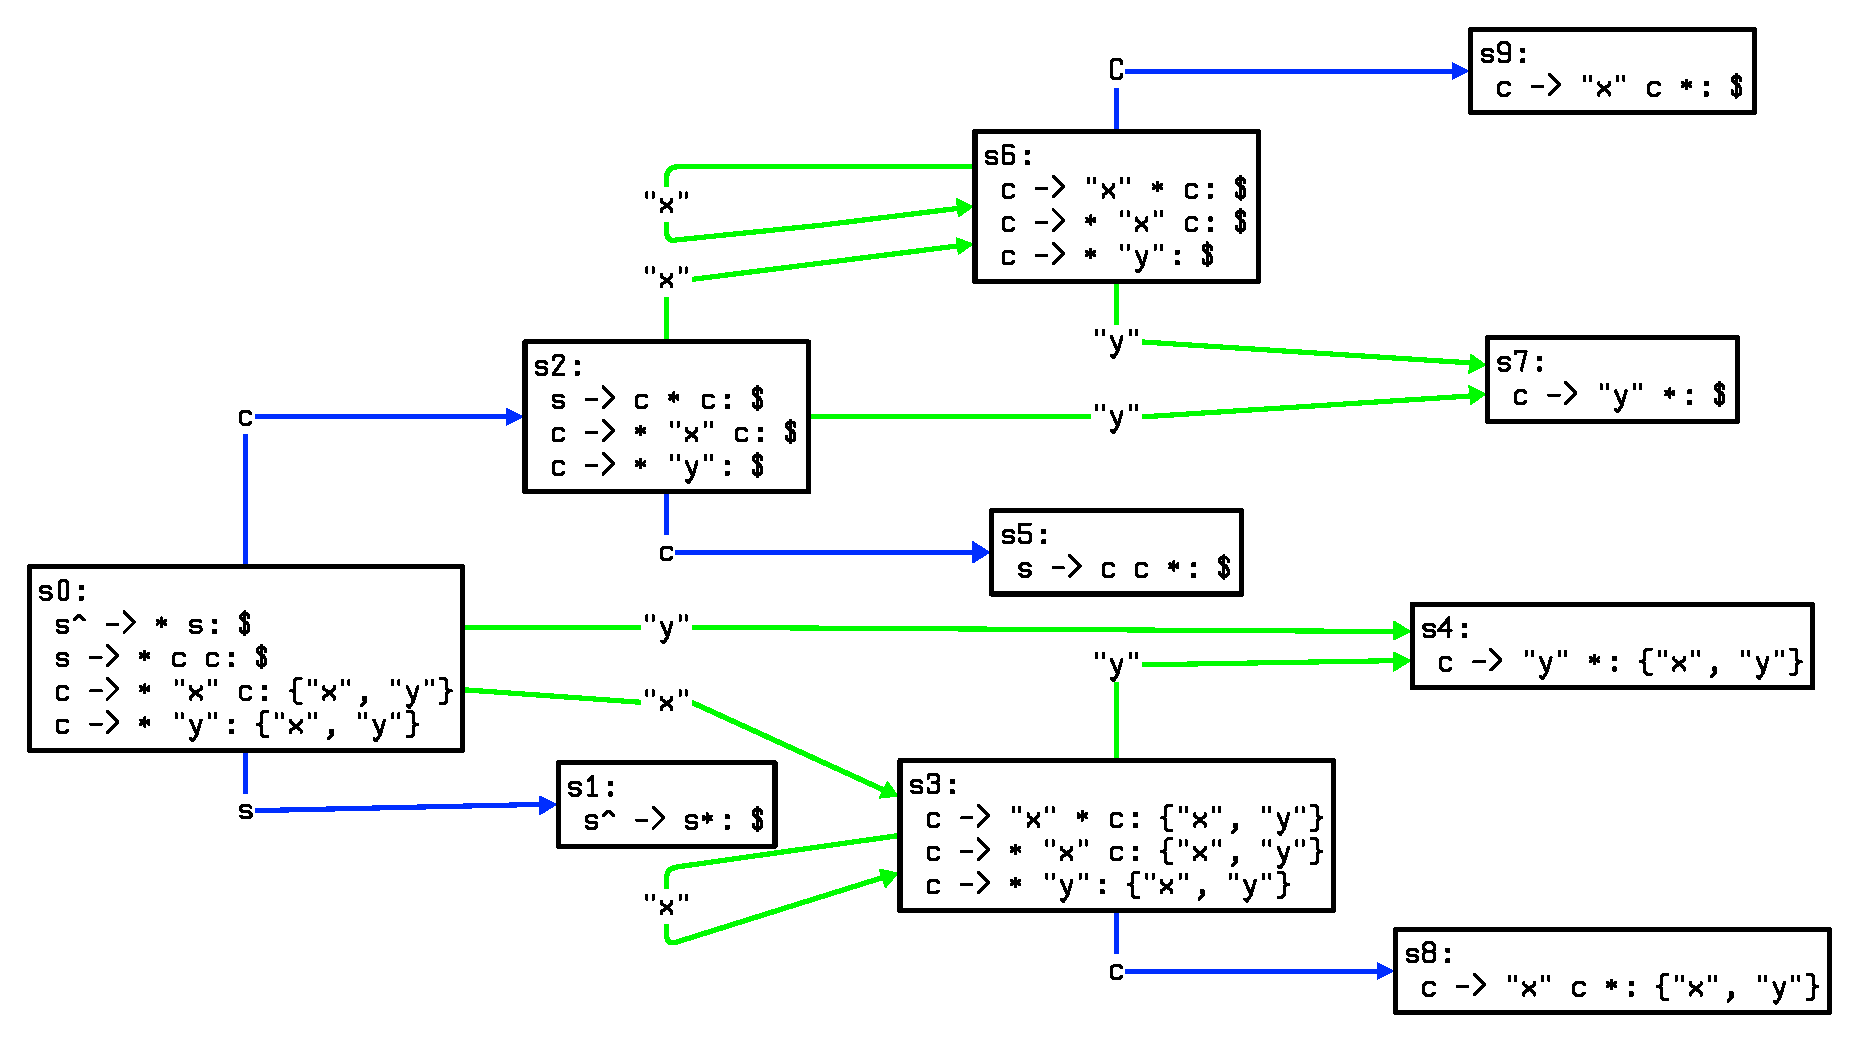
\epsfig{file=Abbildungen/cc-LR.eps, scale=0.5}
      \caption{LR-Goto-Graph f�r die Grammatik aus Abbildung \ref{fig:dragon-book.grammar}.}
  \label{fig:cc-LR.eps}
\end{figure}


Abbildung \ref{fig:cc-LR.eps} zeigt den sogenannten \blue{LR-Goto-Graphen} f�r diese Grammatik.
Die Knoten dieses Graphen sind die Zust�nde.  
Betrachten wir den LR-Goto-Graphen, so stellen wir fest, dass die Zust�nde $s_6$ und
$s_3$ sich nur in den Mengen der Folge-Token unterscheiden, denn es gilt einerseits
\\[0.2cm]
\hspace*{1.3cm}
$s_6 = \Bigl\{ s \rightarrow \saquoted{x} \bullet c: \saquoted{\symbol{36}}, 
                 c \rightarrow \bullet\, \aquoted{x} c:  \saquoted{\symbol{36}},
                 c \rightarrow \bullet\, \aquoted{y}:    \saquoted{\symbol{36}}
       \Bigr\}$, 
\\[0.2cm]
und andererseits haben wir
\\[0.2cm]
\hspace*{1.3cm}
$s_3 = \Bigl\{ s \rightarrow \saquoted{x} \bullet c: \{ \saquoted{x}, \saquoted{y} \}, 
                 c \rightarrow \bullet\, \aquoted{x} c:  \{ \saquoted{x}, \saquoted{y} \},
                 c \rightarrow \bullet\, \aquoted{y}:    \{ \saquoted{x}, \saquoted{y} \}  
       \Bigr\}$.
\\[0.2cm]
Offenbar entsteht die Menge $s_3$ aus der Menge $s_6$ indem �berall $\saquoted{\symbol{36}}$
durch die Menge $\{ \saquoted{x}, \saquoted{y}\}$ ersetzt wird.  Genauso kann die Menge $s_7$ in $s_4$
und $s_9$ in $s_8$ �berf�hrt werden.  Die entscheidende Erkenntnis ist nun, dass die
Funktion $\textsl{goto}()$ unter dieser Art von Transformation invariant ist, denn bei der
Definition dieser Funktion spielt die Menge der Folge-Token keine Rolle.  So sehen wir zum
Beispiel, dass einerseits
\\[0.2cm]
\hspace*{1.3cm}
$\textsl{goto}(s_3, c) = s_8$ \quad und \quad und 
$\textsl{goto}(s_6, c) = s_9$ 
\\[0.2cm]
gilt und dass andererseits der Zustand $s_9$ in den Zustand $s_8$ �bergeht, wenn wir
�berall in $s_9$ das Terminal $\saquoted{\symbol{36}}$ durch die Menge 
 $\{ \saquoted{x}, \saquoted{y}\}$ ersetzen.  Definieren wir den \blue{Kern}
einer Menge von erweiterten markierten Regeln dadurch, dass wir in jeder Regel die Menge
der Folgetoken wegstreichen, und fassen dann Zust�nde mit demselben Kern zusammen, so
erhalten wir den in 
Abbildung \ref{fig:cc-LALR.eps} gezeigten Goto-Graphen.

\begin{figure}[!ht]
\centering
  \hspace*{-0.6cm} 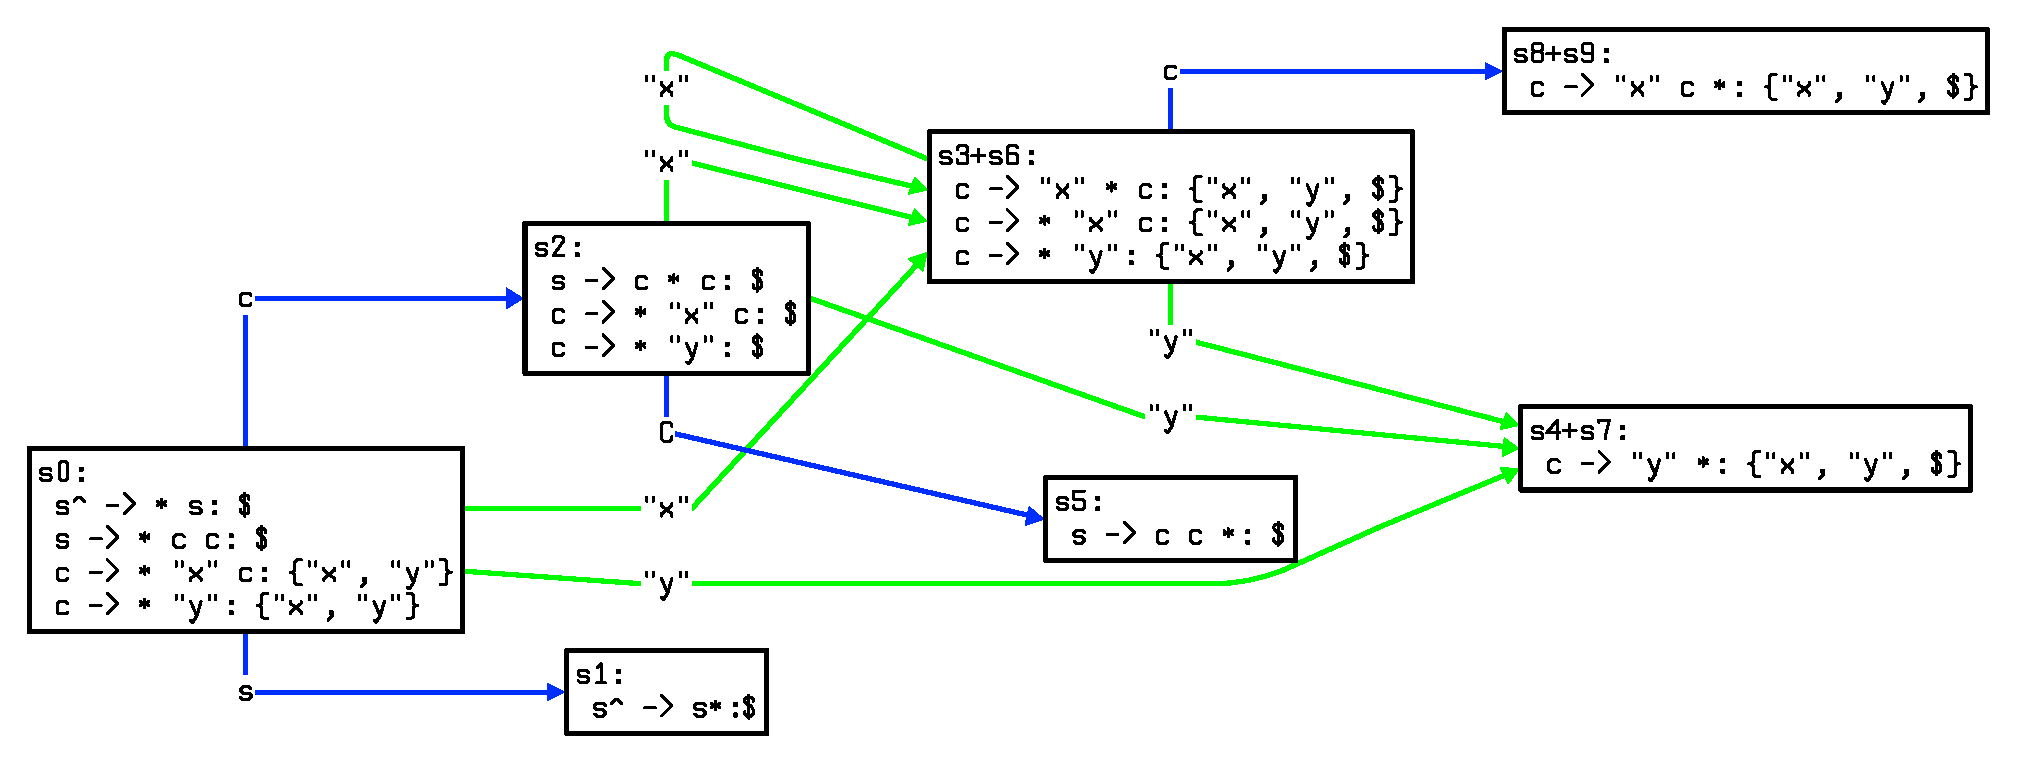
\epsfig{file=Abbildungen/cc-LALR, scale=0.5}
  \caption{Der LALR-Goto-Graph f�r die Grammatik aus Abbildung \ref{fig:dragon-book.grammar}.}
  \label{fig:cc-LALR.eps}
\end{figure}

Um die Beobachtungen, die wir bei der Betrachtung der in Abbildung
\ref{fig:dragon-book.grammar} gezeigten Grammatik gemacht gaben, verallgemeinern und formalisieren zu
k�nnen, definieren wir ein Funktion 
$\textsl{core}()$, die den Kern einer Menge von e.m.R.s berechnet und damit diese Menge in
eine Menge markierter Regeln �berf�hrt: 
\\[0.2cm]
\hspace*{1.3cm}
$\textsl{core}(\mathcal{M}) := 
   \{ a \rightarrow \beta \bullet \gamma \mid (a \rightarrow \beta \bullet \gamma:L) \in \mathcal{M} \}$. 
\\[0.2cm]
Die Funktion $\textsl{core}()$ entfernt also einfach die Menge der Folge-Tokens von den e.m.R.s.
Wir hatten die Funktion $\textsl{goto}()$ f�r eine Menge $\mathcal{M}$ von erweiterten
markierten Regeln und ein Symbol $x$ durch
\\[0.2cm]
\hspace*{1.3cm}
$\textsl{goto}(\mathcal{M}, x) := \textsl{closure}\Bigl( \bigl\{ 
 a \rightarrow \beta\, x \bullet \gamma:L \mid (a \rightarrow \beta \bullet x\, \gamma:L) \in \mathcal{M} 
 \bigr\} \Bigr)
$.
\\[0.2cm]
definiert.  Offenbar spielt die Menge der Folge-Token bei der Berechnung von
$\textsl{goto}(\mathcal{M}, x)$ keine Rolle, formal gilt f�r zwei e.m.R.-Mengen
$\mathcal{M}_1$ und $\mathcal{M}_2$ und ein Symbol $x$ die Formel:
\\[0.2cm]
\hspace*{1.3cm}
$\textsl{core}(\mathcal{M}_1) = \textsl{core}(\mathcal{M}_2) \;\Rightarrow\;
 \textsl{core}(\textsl{goto}(\mathcal{M}_1, x)) = 
 \textsl{core}(\textsl{goto}(\mathcal{M}_2, x))
$.
\vspace*{0.2cm}

F�r zwei e.m.R.-Mengen $\mathcal{M}$ und $\mathcal{N}$, die
den gleichen Kern haben, definieren wir die \blue{erweiterte Vereinigung}  
$\mathcal{M} \uplus \mathcal{N}$ von $\mathcal{M}$ und $\mathcal{N}$ als
\\[0.2cm]
\hspace*{1.3cm}
$\mathcal{M} \uplus \mathcal{N} := 
   \{ a \rightarrow \beta\bullet \gamma:K \cup L \mid 
      (a \rightarrow \beta\bullet \gamma:K) \in \mathcal{M} \;\wedge\;
      (a \rightarrow \beta\bullet \gamma:L) \in \mathcal{N}
   \}
$.
\\[0.2cm] 
Diese Definition verallgemeinern wir zu einer Operation $\biguplus$, 
die auf einer Menge von Mengen von e.m.R.s definiert ist: Ist $\frak{I}$
eine Menge von Mengen von e.m.R.s, die alle den gleichen Kern haben, gilt also
\[ \frak{I} = \{ \mathcal{M}_1, \cdots, \mathcal{M}_k \} \quad \mbox{mit} \quad
   \textsl{core}(\mathcal{M}_i) = \textsl{core}(\mathcal{M}_j) \quad 
   \mbox{f�r alle $i,j\in\{1,\cdots,k\}$,} 
\]
so definieren wir
\[ \biguplus \frak{I} := \mathcal{M}_1 \uplus \cdots \uplus \mathcal{M}_k. 
\]
Es sei nun $\Delta$ die Menge aller Zust�nde eines LR-Parsers.  Dann ist die Menge der Zust�nde des
entsprechenden LALR-Parsers durch die erweiterte Vereinigung der Menge aller der Teilmengen 
von $\Delta$ gegeben, deren Elemente den gleichen Kern haben:
\[ \frak{Q} := \left\{ \biguplus \frak{I} \mid \frak{I} \in 2^\Delta \wedge 
      \forall \mathcal{M},\mathcal{N} \in \frak{I}: \textsl{core}(\mathcal{M}) = \textsl{core}(\mathcal{N}) 
      \wedge \mbox{und $\frak{I}$ maximal} 
   \right\}. 
\]
Die Forderung ``$\frak{I}$ maximal'' dr�ckt in der obigen Definition aus, dass in $\frak{I}$ tats�chlich
\underline{alle} Mengen aus $\Delta$ zusamengefasst sind, die den selben Kern haben.
Die so definierte Menge $\frak{Q}$ ist die Menge der LALR-Zust�nde.  

Als n�chstes �berlegen wir, wie sich die Berechnung von $\textsl{goto}(\mathcal{M},X)$
�ndern muss, wenn $\mathcal{M}$ ein Element der Menge $\frak{Q}$ der LALR-Zust�nde ist.  
Zur Berechnung von $\textsl{goto}(\mathcal{M},X)$ berechnen wir zun�chst die Menge
\\[0.2cm]
\hspace*{1.3cm}
$\textsl{closure}\Bigl( \bigl\{  
  A \rightarrow \alpha X \bullet \beta:L \mid (A \rightarrow \alpha \bullet X \beta:L) \in \mathcal{M} 
  \bigr\} \Bigr)
$.
\\[0.2cm]
Das Problem ist, dass diese Menge im Allgemeinen kein Element der Menge $\frak{Q}$ ist,
denn die Zust�nde in $\frak{Q}$ entstehen ja durch die Zusammenfassung mehrerer LR-Zust�nde.
Die Zust�nde, die bei der Berechnung von $\frak{Q}$ zusammengefasst werden, haben aber alle den selben
Kern.  Daher enth�lt die  Menge
\\[0.2cm]
\hspace*{1.3cm}
$\Bigl\{ q \in \frak{Q} \mid \textsl{core}(q) =
  \textsl{core}\bigl(\textsl{closure}\bigl( \bigl\{  
  a \rightarrow \beta\, x \bullet \gamma:L \mid (a \rightarrow \beta \bullet x\, \gamma:L) \in \mathcal{M} 
  \bigr\} \bigr)\bigr)
  \Bigr\}
$
\\[0.2cm]
genau ein Element und dieses Element ist der Wert von $\textsl{goto}(\mathcal{M}, X)$.  Folglich
k�nnen wir  
\\[0.2cm]
\hspace*{1.3cm}
$\ds\textsl{goto}(\mathcal{M}, X) := \textsl{arb}\Bigl(\Bigl\{ q \in \frak{Q} \mid \textsl{core}(q) =
  \textsl{core}\Bigl(\textsl{closure}\Bigl( \bigl\{  
  a \rightarrow \beta\, X \bullet \gamma:L \mid (a \rightarrow \beta \bullet X\, \gamma:L) \in \mathcal{M} 
  \bigr\} \Bigr)\Bigr)
  \Bigr\} \Bigr)
$
\\[0.2cm]
setzen.  Die hier verwendete Funktion $\textsl{arb}()$ dient dazu, ein beliebiges Element aus einer Menge
zu extrahieren.  Da die Menge, aus der hier das Element extrahiert wird, genau ein Element enth�lt, ist
$\textsl{goto}(\mathcal{M}, x)$ wohldefiniert.
Die Berechnung des Ausdrucks $\textsl{action}(\mathcal{M}, t)$ �ndert sich gegen�ber der Berechnung f�r
einen LR-Parser nicht. 

\section{Vergleich von SLR-, LR- und LALR-Parsern}
Wir wollen nun die verschiedenen Methoden, mit denen wir in diesem Kapitel
Shift-Reduce-Parser konstruiert haben, vergleichen.  Wir nennen eine Sprache $\mathcal{L}$
eine \blue{SLR-Sprache}, wenn $\mathcal{L}$ von einem SLR-Parser erkannt werden kann.
Die Begriffe \blue{kanonische LR-Sprache} und \blue{LALR-Sprache} werden analog definiert.
 Zwischen diesen Sprachen bestehen die folgende Beziehungen:
\\[0.2cm]
\hspace*{1.3cm}
\blue{SLR-Sprache} $\subsetneq$ \blue{LALR-Sprache} $\subsetneq$ \blue{kanonische LR-Sprache} 
\hspace*{\fill} $(\star)$
\\[0.2cm]
Diese Inklusionen sind leicht zu verstehen:  Bei der Definition der LR-Parser hatten wir
zu den markierten Regeln  Mengen von Folge-Token hinzugef�gt.  Dadurch war
es m�glich, in bestimmten F�llen Shift-Reduce- und Reduce-Reduce-Konflikte zu vermeiden.
Da die Zustands-Mengen der kanonischen LR-Parser unter Umst�nden sehr gro� werden k�nnen,
hatten wir dann wieder solche Mengen von erweiterten markierten Regeln zusammengefasst,
f�r die die Menge der Folge-Token identisch war.  So hatten wir die LALR-Parser
erhalten.  Durch die Zusammenfassung von Regel-Menge k�nnen wir
uns allerdings in bestimmten F�llen Reduce-Reduce-Konflikte einhandeln, so dass die 
Menge der LALR-Sprachen eine Untermenge der kanonischen LR-Sprachen ist.

Wir werden in den folgenden Unterabschnitten zeigen, dass die Inklusionen in $(\star)$ echt sind.  

\subsection{\blue{SLR-Sprache} $\subsetneq$ \blue{LALR-Sprache}}
Die Zust�nde eines LALR-Parsers enthalten gegen�ber den Zust�nden eines SLR-Parsers noch
Mengen von Folge-Token.  Damit sind LALR-Parser mindestens genauso m�chtig wie SLR-Parser.
Wir zeigen nun, dass LALR-Parser tats�chlich m�chtiger als SLR-Parser sind.  Um diese
Behauptung zu belegen, pr�sentieren wir eine Grammatik, f�r die es zwar einen LALR-Parser,
aber keinen SLR-Parser gibt.  Wir hatten auf Seite \pageref{fig:reduce-reduce-conflict.grammar}
gesehen, dass die Grammatik
\\[0.2cm]
\hspace*{1.3cm}
$s \;\rightarrow\; a \aquoted{x} a \aquoted{y} \mid b \aquoted{y} b \aquoted{x}$, \quad
$a \;\rightarrow\;\varepsilon$, \quad
$b \;\rightarrow\; \varepsilon$
\\[0.2cm]
keine SLR-Grammatik ist.  Sp�ter hatten wir gesehen, dass diese Grammatik von einem
kanonischen LR-Parser geparst werden kann.  Wir zeigen nun, dass diese Grammatik auch von
einem LALR-Parser geparst werden kann.  Dazu berechnen wir die Menge der LALR-Zust�nde.
Dazu ist zun�chst die Menge der kanonischen LR-Zust�nde zu berechnen.  Diese Berechnung
hatten wir bereits fr�her durchgef�hrt und dabei die folgenden Zust�nde erhalten:
\begin{enumerate}
\item $s_0  = \bigl\{ \widehat{s} \rightarrow \bullet\, s:\symbol{36},
                     s \rightarrow \bullet\, a \saquoted{x} a \saquoted{y}:\symbol{36},
                     s \rightarrow \bullet\, b \saquoted{y} b \saquoted{x}:\symbol{36},
                     a \rightarrow \bullet\,: \saquoted{x},
                     b \rightarrow \bullet\,: \saquoted{y}
              \bigr\}
      $,
\item $s_1 = \bigl\{ s \rightarrow a \bullet \saquoted{x} a \saquoted{y}:\symbol{36} \bigr\}$,
\item $s_2 = \bigl\{ \widehat{s} \rightarrow s \bullet:\symbol{36} \bigr\}$,
\item $s_3 = \bigl\{ s \rightarrow b \bullet \saquoted{y} b \saquoted{x}: \symbol{36} \bigr\}$,
\item $s_4 = \bigl\{ s \rightarrow b \saquoted{y} \bullet b \saquoted{x}: \symbol{36},
                     b \rightarrow \bullet\,: \saquoted{x}
             \bigr\}
      $,
\item $s_5 = \bigl\{ s \rightarrow b \saquoted{y} b \bullet \saquoted{x}: \symbol{36} \bigr\}$,
\item $s_6 = \bigl\{ s \rightarrow b \saquoted{y} b \saquoted{x} \bullet: \symbol{36} \bigr\}$,
\item $s_7 = \bigl\{ s \rightarrow a \saquoted{x} \bullet a \saquoted{y}:\symbol{36},
                     a \rightarrow \bullet\,: \saquoted{y}
              \bigr\}
      $,
\item $s_8 = \bigl\{ s \rightarrow a \saquoted{x} a \bullet \saquoted{y}:\symbol{36} \bigr\}$,
\item $s_9 = \bigl\{ s \rightarrow a \saquoted{x} a \saquoted{y} \bullet :\symbol{36} \bigr\}$.
\end{enumerate}
Wir stellen fest, dass die Kerne aller hier aufgelisteten Zust�nde verschieden sind.
Damit stimmt bei dieser Grammatik die Menge der Zust�nde des LALR-Parser mit der Menge der
Zust�nde des kanonischen LR-Parsers �berein.  Daraus folgt, dass es auch bei
den LALR-Zust�nden keine Konflikte gibt, denn beim �bergang von kanonischen LR-Parsern zu
LALR-Parsern haben wir lediglich Zust�nde mit gleichem Kern zusammengefasst, die
Definition der Funktionen $\textsl{goto}()$ und $\textsl{action}()$ blieb unver�ndert.

\subsection{\blue{LALR-Sprache} $\subsetneq$ \blue{kanonische LR-Sprache}}
Wir hatten LALR-Parser dadurch definiert, dass wir verschiedene Zust�nde eines kanonischen LR-Parsers
zusammengefasst haben.  Damit ist klar, dass kanonische LR-Parser mindestens so m�chtig
sind wie LALR-Parser.  Um zu zeigen, dass kanonische LR-Parser tats�chlich m�chtiger sind
als LALR-Parser, ben�tigen wir eine Grammatik, f�r die sich zwar ein kanonischer LR-Parser,
aber kein LALR-Parser erzeugen l�sst.  Abbildung \ref{fig:lr-but-notlalr.g} zeigt eine
solche Grammatik, die ich dem Drachenbuch entnommen habe.

\begin{figure}[htbp]
  \begin{center}    
  \framebox{
  \framebox{
  \begin{minipage}[t]{5.5cm}
    \vspace*{-0.3cm}

  \begin{eqnarray*}
  s  & \rightarrow & \aquoted{v} a \aquoted{y} \\
     & \mid        & \aquoted{w} b \aquoted{y} \\
     & \mid        & \aquoted{v} b \aquoted{z} \\
     & \mid        & \aquoted{w} a \aquoted{z} \\[0.1cm]
  a  & \rightarrow & \aquoted{x}              \\[0.1cm]
  b  & \rightarrow & \aquoted{x}              
  \end{eqnarray*}
  \vspace*{-0.5cm}

  \end{minipage}}}
  \vspace*{-0.3cm}

  \end{center}
  \caption{Eine kanonische LR-Grammatik, die keine LALR-Grammatik ist.}
  \label{fig:lr-but-notlalr.g}
\end{figure}

Wir berechnen zun�chst die Menge der Zust�nde eines kanonischen LR-Parsers f�r diese
Grammatik.  Wir erhalten dabei die folgende Mengen von erweiterten markierten Regeln:
\begin{enumerate}
\item $s_0 = \textsl{closure}(\widehat{s} \rightarrow \bullet\, \;s: \symbol{36}) =
       \{
       \begin{array}[t]{lcl}
         \widehat{s} & \rightarrow & \bullet \;s: \symbol{36},                \\
         s           & \rightarrow & \bullet \saquoted{v} a \saquoted{y}: \symbol{36}, \\
         s           & \rightarrow & \bullet \saquoted{v} b \saquoted{z}: \symbol{36}, \\
         s           & \rightarrow & \bullet \saquoted{w} a \saquoted{z}: \symbol{36}, \\
         s           & \rightarrow & \bullet \saquoted{w} b \saquoted{y}: \symbol{36}\;\},
        \end{array}
       $
\item $s_1 = \textsl{goto}(s_0, s) =\{ \widehat{s} \rightarrow s \bullet: \symbol{36} \}$
\item $s_2 = \textsl{goto}(s_0, \aquoted{v}) = \{ 
       \begin{array}[t]{lcl}
        s & \rightarrow & \saquoted{v} \bullet b \saquoted{z}: \symbol{36}, \\
        s & \rightarrow & \saquoted{v} \bullet a \saquoted{y}: \symbol{36}, \\
        a & \rightarrow & \bullet \saquoted{x}: \saquoted{y}, \\
        b & \rightarrow & \bullet \saquoted{x}: \saquoted{z}\; \},
       \end{array}
      $
\item $s_3 = \textsl{goto}(s_0, \aquoted{w}) = \{ 
       \begin{array}[t]{lcl}
       s & \rightarrow & \saquoted{w} \bullet a \saquoted{z}: \symbol{36},  \\
       s & \rightarrow & \saquoted{w} \bullet b \saquoted{y}: \symbol{36},  \\
       a & \rightarrow & \bullet \saquoted{x}: \saquoted{z},                \\
       b & \rightarrow & \bullet \saquoted{x}: \saquoted{y}\; \},
       \end{array}
      $
\item $s_4 = \textsl{goto}(s_2, \aquoted{x}) =
             \{ a \rightarrow \saquoted{x} \bullet: \saquoted{y},\;
                b \rightarrow \saquoted{x} \bullet: \saquoted{z} \}$,
\item $s_5 = \textsl{goto}(s_3, \aquoted{x}) =
             \{ a \rightarrow \saquoted{x} \bullet: \saquoted{z},\,
                b \rightarrow \saquoted{x} \bullet: \saquoted{y} \}$,
\item $s_6 = \textsl{goto}(s_2, a) =
             \{ s \rightarrow \saquoted{v} a \bullet \saquoted{y}: \symbol{36} \}$,
\item $s_7 = \textsl{goto}(s_6, \aquoted{y}) =
             \{ s \rightarrow \saquoted{v} a \saquoted{y} \bullet: \symbol{36} \}$,
\item $s_8 = \textsl{goto}(s_2, b) =
             \{ s \rightarrow \saquoted{v} b \bullet \saquoted{z}: \symbol{36} \}$,
\item $s_9 = \textsl{goto}(s_8, \aquoted{z}) =
             \{ s \rightarrow \saquoted{v} b \saquoted{z} \bullet: \symbol{36} \}$,
\item $s_{10} = \textsl{goto}(s_3, a) =
                \{ s \rightarrow \saquoted{w} a \bullet \saquoted{z}: \symbol{36} \}$,
\item $s_{11} = \textsl{goto}(s_{10}, \aquoted{z}) =
                \{ s \rightarrow \saquoted{w} a \saquoted{z} \bullet: \symbol{36} \}$,
\item $s_{12} = \textsl{goto}(s_3, b) =
                \{ s \rightarrow \saquoted{w} b \bullet \saquoted{y}: \symbol{36} \}$,
\item $s_{13} = \textsl{goto}(s_{12}, \aquoted{y}) =
                \{ s \rightarrow \saquoted{w} b \saquoted{y} \bullet: \symbol{36} \}$.
\end{enumerate}
Die einzigen Zust�nde, bei denen es Konflikte geben k�nnte, sind die Mengen $s_4$ und
$s_5$, denn hier sind prinzipiell sowohl Reduktionen mit der Regel
\\[0.2cm]
\hspace*{1.3cm}
$a \rightarrow \saquoted{x}$ \quad als auch mit \quad
$b \rightarrow \saquoted{x}$
\\[0.2cm]
m�glich.  Da allerdings die Mengen der Folge-Token einen leeren Durchschnitt haben, gibt
es tats�chlich keinen Konflikt und die Grammatik ist eine kanonische LR-Grammatik.

Wir berechnen als n�chstes die LALR-Zust�nde der oben angegebenen Grammatik.  Die einzigen
Zust�nde, die einen gemeinsamen Kern haben, sind die beiden Zust�nde $s_4$ und $s_5$, denn
es gilt
\\[0.2cm]
\hspace*{1.3cm}
$\textsl{core}(s_4) = \{ a \rightarrow \saquoted{x} \bullet,\;
                b \rightarrow \saquoted{x} \bullet \} = \textsl{core}(s_5)$.
\\[0.2cm]
Bei der Berechnung der LALR-Zust�nde werden diese beiden Zust�nde zu einem Zustand
$s_{\{4,5\}}$ zusammengefasst.  Dieser neue Zustand hat die Form
\\[0.2cm]
\hspace*{1.3cm}
$s_{\{4,5\}} = \bigl\{ A \rightarrow \saquoted{x} \bullet: \{\saquoted{y}, \saquoted{z} \},\;
                       B \rightarrow \saquoted{x} \bullet: \{\saquoted{y}, \saquoted{z} \} \bigr\}$.
\\[0.2cm]
Hier gibt es offensichtlich  einen Reduce-Reduce-Konflikt, denn einerseits haben wir
\\[0.2cm]
\hspace*{1.3cm}
$\textsl{action}(s_{\{4,5\}}, \saquoted{y}) = \pair(\textsl{reduce}, A \rightarrow \saquoted{x})$,
\\[0.2cm]
andererseits gilt aber auch
\\[0.2cm]
\hspace*{1.3cm}
$\textsl{action}(s_{\{4,5\}}, \saquoted{y}) = \pair(\textsl{reduce}, B \rightarrow \saquoted{x})$.

\exercise
Es sei $G = \langle V, T, R, s \rangle$ eine LR-Grammatik und $\mathcal{N}$ sei die Menge der
LALR-Zust�nde der Grammatik.  �berlegen Sie, warum es in der Menge $\mathcal{N}$ keine
Shift-Reduce-Konflikte geben kann.  \eox


\paragraph{Historical Notes}
The theory of LALR parsing is due to Franklin L.~DeRemer \cite{deRemer:71}.  At the time of its
invention,  the space savings of LALR parsing in comparison to LR parsing were crucial.  


\subsection{Bewertung der verschiedenen Methoden}
F�r die Praxis sind SLR-Parser nicht ausreichend, denn es gibt eine Reihe praktisch
relevanter Sprach-Konstrukte, f�r die sich kein SLR-Parser erzeugen l�sst.  Kanonische
LR-Parser sind wesentlich m�chtiger, ben�tigen allerdings oft deutlich mehr Zust�nde. 
Hier stellen LALR-Parser einen Kompromiss dar:  Einerseits sind LALR-Sprachen fast so
ausdrucksstark  wie kanonische LR-Sprachen, andererseits liegt der Speicherbedarf von
LALR-Parsern in der gleichen Gr��enordnung wie der Speicherbedarf von SLR-Parsern.  Beispielsweise
hat die SLR-Parse-Tabelle f�r die Sprache \texttt{C} insgesamt 349 Zust�nde, die entsprechende
LR-Parse-Tabelle kommt auf 1572 Zust�nde, w�hrend der LALR-Parser mit 350 Zust�nden auskommt und damit nur
einen Zustand mehr als der SLR-Parser hat.  
In den heute in der Regel zur Verf�gung stehenden Hauptspeichern lassen sich allerdings
auch kanonische LR-Parser meist m�helos unterbringen, so dass es eigentlich keinen zwingenden
Grund mehr gibt, statt eines LR-Parsers einen LALR-Parser einzusetzen.  

Andererseits wird niemand einen LALR-Parser oder einen kanonischen LR-Parser von Hand
programmieren wollen.  Stattdessen werden Sie sp�ter einen Parser-Generator wie \textsl{Bison}
oder \textsl{JavaCup} einsetzen, der Ihnen einen  Parser generiert.  Das Werkzeug Bison
ist ein Parser-Generator f�r \texttt{C}, \texttt{C++} und bietet auch eine, allerdings leider noch
experimentelle, Unterst�tzung f�r \textsl{Java},
w�hrend \textsl{JavaCup} auf die Sprache \textsl{Java} beschr�nkt ist.  Falls Sie
\textsl{JavaCup} benutzen, haben Sie keine Wahl, denn dieses Werkzeug erzeugt immer einen
LALR-Parser.  Bei \href{http://www.gnu.org/software/bison/manual/bison.html}{\textsl{Bison}} ist es
ab der Version 3.0  auch m�glich, einen LR-Parser zu erzeugen.



%%% Local Variables: 
%%% mode: latex
%%% TeX-master: "formal-languages"
%%% End: 

\chapter{Using \textsc{Ply} as a Parser Generator  \label{chapter:ply}}
Most\footnote{The programming language \texttt{C++} is a noteable exception.} modern programming languages can
be parsed using an LALR-Parser.  As this lesson is based on the programming language \textsl{Python}, this
chapter discusses how the parser generator \href{https://www.dabeaz.com/ply/}{\textsc{Ply}} can be used to
generate a parser for any language that has an LALR grammar.  In Chapter \ref{chapter:ply-lex} we have already
seen how \textsc{Ply} can be used to generate a scanner.  This chapter focuses on the parser-generating aspect
of \textsc{Ply}.   If you haven't done so already, you can install \textsc{Ply} via \texttt{anaconda} as follows:
\\[0.2cm]
\hspace*{1.3cm}
\texttt{conda install -c conda-forge ply}


\section{A Simple Example}
Figure \ref{fig:calculator.g} on page \pageref{fig:calculator.g} shows the grammar of a simple 
\blue{symbolic calculator}.  This grammar is similar to the grammar shown in Figure \ref{fig:Program.g4} on page
\pageref{fig:Program.g4} in Chapter \ref{chapter:antlr}. 

\begin{figure}[!ht]

  \begin{center}    
  \framebox{
  \framebox{
  \begin{minipage}[t]{9cm}
  \begin{eqnarray*}
  \textsl{stmnt}   & \rightarrow & \;\textsc{Identifier} \quoted{:=} \textsl{expr} \quoted{;}\\
                   & \mid        & \;\textsl{expr} \quoted{;}                   \\[0.2cm]
  \textsl{expr}    & \rightarrow & \;\textsl{expr} \quoted{+} \textsl{product}  \\
                   & \mid        & \;\textsl{expr} \quoted{-} \textsl{product}  \\
                   & \mid        & \;\textsl{product}                           \\[0.2cm]
  \textsl{product} & \rightarrow & \;\textsl{product} \quoted{*} \textsl{factor}\\
                   & \mid        & \;\textsl{product} \quoted{/} \textsl{factor}\\
                   & \mid        & \;\textsl{factor}                            \\[0.2cm]
  \textsl{factor}  & \rightarrow &   \quoted{(} \textsl{expr} \quoted{)}        \\
                   & \mid        & \;\textsc{Number}                            \\
                   & \mid        & \;\textsc{Identifier}                        
  \end{eqnarray*}
  \vspace*{-0.5cm}
  \end{minipage}}}
  \end{center}
  \caption{A grammar for a symbolic calculator.}
  \label{fig:calculator.g}
\end{figure}

In order to generate a symbolic calculator that is based on this grammar we first need to implement a scanner.
Figure \ref{fig:Symbolic-Calculator.ipynb:lex} shows how to specify an appropriate scanner with \textsc{Ply}.
As we have discussed scanner generation with \textsc{Ply} at length in Chapter \ref{chapter:ply-lex} there is
no need for further discussions here.

\begin{figure}[!ht]
\centering
\begin{minted}[ frame        = lines, 
                framesep     = 0.3cm, 
                bgcolor      = sepia,
                numbers      = left,
                numbersep    = -0.2cm,
                xleftmargin  = 0.8cm,
                xrightmargin = 0.8cm,
              ]{python3}
    import ply.lex as lex
    
    tokens = [ 'NUMBER', 'IDENTIFIER', 'ASSIGN_OP' ]
    
    def t_NUMBER(t):
        r'0|[1-9][0-9]*(\.[0-9]+)?([eE][+-]?([1-9][0-9]*))?'
        t.value = float(t.value)
        return t
    
    def t_IDENTIFIER(t):
        r'[a-zA-Z][a-zA-Z0-9_]*'
        return t
    
    def t_ASSIGN_OP(t):
        r':='
        return t
    
    literals = ['+', '-', '*', '/', '(', ')', ';']
    
    t_ignore  = ' \t'
    
    def t_error(t):
        print(f"Illegal character '{t.value[0]}'")
        t.lexer.skip(1)
    
    lexer = lex.lex()
\end{minted}
\vspace*{-0.3cm}
\caption{A scanner for the symbolic calculator.}
\label{fig:Symbolic-Calculator.ipynb:lex}
\end{figure}

\begin{figure}[!ht]
\centering
\begin{minted}[ frame        = lines, 
                framesep     = 0.3cm, 
                bgcolor      = sepia,
                numbers      = left,
                numbersep    = -0.2cm,
                xleftmargin  = 0.8cm,
                xrightmargin = 0.8cm,
              ]{python3}
    import ply.yacc as yacc
    
    start = 'stmnt'
    
    def p_stmnt_assign(p):
        "stmnt : IDENTIFIER ASSIGN_OP expr ';'"
        Names2Values[p[1]] = p[3]
    
    def p_stmnt_expr(p):
        "stmnt : expr ';'"
        print(p[1])
    
    def p_expr_plus(p):
        "expr : expr '+' prod"
        p[0] = p[1] + p[3]
        
    def p_expr_minus(p):
        "expr : expr '-' prod"
        p[0] = p[1] - p[3]
        
    def p_expr_prod(p):
        "expr : prod"
        p[0] = p[1]
    
    def p_prod_mult(p):
        "prod : prod '*' factor"
        p[0] = p[1] * p[3]
        
    def p_prod_div(p):
        "prod : prod '/' factor"
        p[0] = p[1] / p[3]
        
    def p_prod_factor(p):
        "prod : factor"
        p[0] = p[1]
    
    def p_factor_group(p):
        "factor : '(' expr ')'"
        p[0] = p[2]
    
    def p_factor_number(p):
        "factor : NUMBER"
        p[0] = p[1]
    
    def p_factor_id(p):
        "factor : IDENTIFIER"
        p[0] = Names2Values.get(p[1], float('nan'))
\end{minted}
\vspace*{-0.3cm}
\caption{A scanner for the symbolic calculator, part 1.}
\label{fig:Symbolic-Calculator.ipynb:yacc}
\end{figure}

Figure \ref{fig:Symbolic-Calculator.ipynb:yacc} on page \pageref{fig:Symbolic-Calculator.ipynb:yacc} shows how the
grammar is implemented in \textsc{Ply}.  We discuss it line by line.
\begin{enumerate}
\item Line 1 imports the module \texttt{ply.yacc}.  This module contains the function \texttt{ply.yacc.yacc}
      which is responsible for computing the parse table. The name \blue{yacc} is a homage to the Unix tool
      \href{https://en.wikipedia.org/wiki/Yacc}{\textsc{Yacc}}, which is a popular parser generator for the language
      \texttt{C} and, furthermore, is part of the standard utilities of the Unix operating system.
\item Line 3 specifies that the syntactical variable \texttt{stmnt} is the \blue{start symbol} of the grammar.
\item Line 5 -- 7 define the function \texttt{p\_stmnt\_assign} which implements the grammar rule
      \\[0.2cm]
      \hspace*{1.3cm}
      $\textsl{stmnt} \rightarrow \textsc{Identifier} \quoted{:=} \textsl{expr}$.
      \\[0.2cm]
      Note that this grammar rule itself is represented by the \blue{document string} of the function
      \texttt{p\_stmnt\_assign}.  In general, if
      \\[0.2cm]
      \hspace*{1.3cm}
      $v \rightarrow \alpha$
      \\[0.2cm]
      is a grammar rule, then this grammar rule is represented by a function that has the name
      \texttt{p\_$v$\_$s$}.  Here, the prefix ``\texttt{p\_}'' specifies that the function implements 
      a grammar rule (the \texttt{p} is short for \blue{parser}), $v$ should\footnote{
        This is just a convention. Technically, $v$ can be any string that is a valid \textsl{Python}
        identifier.
      }
      be the name of the variable
      defined by this grammar rule, and $s$ is a string chosen by the user to distinguish between different
      grammar rules for the same variable.  Of course, $s$ has to be chosen in a way such that the string
      \texttt{p\_$v$\_$s$} is a legal \textsl{Python} identifier.

      The function always takes one argument \texttt{p}.  This argument is a sequence of objects that can be
      indexed with array notation. If the grammar rule defining $v$ has the form
      \\[0.2cm]
      \hspace*{1.3cm}
      $v \rightarrow X_1 \cdots X_n$,
      \\[0.2cm]
      then this sequence has a length of $n+1$.  If $X_i$ is a token, then \texttt{p[$i$]} is the property
      with name \texttt{value} that is associated with this token.  Often, this value is just a string, but it
      can also be a number.  If $X_i$ is a variable, then  \texttt{p[$i$]} is the value that is returned
      when $X_i$ is recognized.  The value associated with the variable $v$ is stored in the location
      \texttt{p[0]}.  In the grammar rule shown in line 5--7, we have not assigned any value to \texttt{p[0]} and
      therefore there is no value associated with the syntactical variable \texttt{stmnt} that is defined by
      this grammar rule.

      \underline{\textbf{Note:}} Line 6 shows how a grammar rule is represented for \textsc{Ply}.
      A grammar rule of the form 
      \\[0.2cm]
      \hspace*{1.3cm}
      $v \rightarrow X_1 \cdots X_n$
      \\[0.2cm]
      is represented as the string:
      \\[0.2cm]
      \hspace*{1.3cm}
      \texttt{"$v$ : $X_1$ $\cdots$ $X_n$"}
      \\[0.2cm]
      It is very \red{\underline{im}p\underline{ortant}} that the character ``\texttt{:}'' is
      surrounded by space characters.  Otherwise, the parser generator does not work but rather generates error
      messages that are difficult to understand. 

      The function \texttt{p\_stmnt\_assign} has the task of evaluating the expression that is on the right
      hand side of the assignment operator ``\texttt{:=}''.  The result of this evaluation is then stored in the
      dictionary \texttt{Names2Values}.  The key that is used is the name of the identifier to the left of the
      assignment operator.
\item The function in line 9 -- 11 implements the grammar rule
      \\[0.2cm]
      \hspace*{1.3cm}
      $\textsl{stmnt} \rightarrow \textsl{expr} \quoted{;}$.
      \\[0.2cm]
      The rule is implemented by evaluating the expression and then printing it.
\item The function \texttt{p\_expr\_plus} implements the grammar rule
      \\[0.2cm]
      \hspace*{1.3cm}
      $\textsl{expr} \rightarrow \textsl{expr} \quoted{+} \textsl{prod}$.
      \\[0.2cm]
      It is implemented by evaluating the expression to the left of the operator ``\texttt{+}'', which is
      stored in \texttt{p[1]}, and the product to the right of this operator, which is stored in \texttt{p[3]},
      and then adding the corresponding values.  Finally, the resulting sum is stored in \texttt{p[0]} so that
      it is available later as the value of the expression that has been parsed.

      The remaining functions are similar to the ones that are discussed above.
\end{enumerate}

\begin{figure}[!ht]
\centering
\begin{minted}[ frame        = lines, 
                framesep     = 0.3cm, 
                bgcolor      = sepia,
                numbers      = left,
                numbersep    = -0.2cm,
                xleftmargin  = 0.8cm,
                xrightmargin = 0.8cm,
              ]{python3}
    def p_error(p):
        if p:
            print(f'Syntax error at {p.value} in line {p.lexer.lineno}.')
        else:
            print('Syntax error at end of input.')
        
    parser = yacc.yacc(write_tables=False, debug=True)

    Names2Values = {}
    
    def main():
        while True:
            s = input('calc > ')
            if s == '':
                break
            yacc.parse(s)
\end{minted}
\vspace*{-0.3cm}
\caption{A scanner for the symbolic calculator, part 2.}
\label{fig:Symbolic-Calculator.ipynb:yacc2}
\end{figure}
\FloatBarrier

\noindent
Figure \ref{fig:Symbolic-Calculator.ipynb:yacc2} on page \pageref{fig:Symbolic-Calculator.ipynb:yacc2}
is discussed next.
\begin{enumerate}
\item Line 1 -- 5 shows the function \texttt{p\_error} which is used to print error messages in the case that
      the input can not be parsed because of a syntax error.  The argument \texttt{p} is the token $t$ that
      caused the entry $\texttt{action}(s, t)$ in the action table to be undefined.
      If the syntax error happens at the end of the input, \texttt{p} has the value \texttt{None}.
\item Line 7 generates the parser.
      \begin{enumerate}[(a)]
      \item The first argument \texttt{write\_tables} has to be set to \texttt{False} to prevent an obscure bug.
      \item The argument \texttt{debug} has to be set to \texttt{True} if we want to dump the parse table
            to the disk.  The parse table is then written to the file \texttt{parser.out}.
      \end{enumerate}
\item Line 9 initializes the dictionary \texttt{Names2Values}.  For every identifier $x$ defined interactively,
      \texttt{Names2Values[$x$]} is the value associated with $x$.
\item The function \texttt{main} is used as a driver for the parser.  It reads a string \texttt{s}
      from the command line and tries to parse \texttt{s} using the function \texttt{yacc.parse}.
      The function \texttt{yacc.parse} is generated behind the scenes when the function \texttt{yacc.yacc} is
      invoked in line 7. 
\end{enumerate}


\section{Shift-Reduce and Reduce-Reduce Conflicts}
In this section we show how shift-reduce and reduce-reduce conflicts are dealt with in \textsc{Ply}.
Figure \ref{fig:Conflicts.ipynb} on page \pageref{fig:Conflicts.ipynb} shows a grammar for arithmetical
expressions that is ambiguous because it does not specify the precedence of the different arithmetical
operators.  


\begin{figure}[!ht]
\centering
\begin{Verbatim}[ frame         = lines, 
                  framesep      = 0.3cm, 
                  labelposition = bottomline,
                  numbers       = left,
                  numbersep     = -0.2cm,
                  xleftmargin   = 0.8cm,
                  xrightmargin  = 0.8cm,
                  commandchars  = \\\{\}
                ]
    expr : expr '+' expr
         | expr '*' expr
         | NUMBER      
\end{Verbatim}
\vspace*{-0.3cm}
\caption{An ambiguous grammar for arithmetical expressions.}
\label{fig:Conflicts.ipynb}
\end{figure}
\FloatBarrier

\noindent
This grammar does not specify whether the string
\\[0.2cm]
\hspace*{1.3cm} 
``\texttt{1 + 2 * 3}'' \quad is interpreted as \quad  ``\texttt{(1 + 2) * 3}'' \quad or as \quad ``\texttt{1 +
  (2 * 3)}''. 
\\[0.2cm]
Since every LALR is unambiguous, but the grammar shown in Figure \ref{fig:Conflicts.ipynb} is ambiguous,  it
has to have shift-reduce or reduce-reduce conflicts.  This grammar is part of the jupyter notebook 
\\[0.2cm]
\hspace*{1.3cm}
\href{https://github.com/karlstroetmann/Formal-Languages/tree/master/Ply/Conflicts.ipynb}{Formal-Languages/tree/master/Ply/Conflicts.ipynb}.


\begin{figure}[!ht]
\centering
\begin{Verbatim}[ frame         = lines, 
                  framesep      = 0.3cm, 
                  labelposition = bottomline,
                  numbers       = left,
                  numbersep     = -0.2cm,
                  xleftmargin   = 0.8cm,
                  xrightmargin  = 0.8cm,
                  commandchars  = \\\{\}
                ]
    state 5
    
        (1) expr -> expr + expr .
        (1) expr -> expr . + expr
        (2) expr -> expr . * expr
    
      ! shift/reduce conflict for + resolved as shift
      ! shift/reduce conflict for * resolved as shift
        $end            reduce using rule 1 (expr -> expr + expr .)
        +               shift and go to state 3
        *               shift and go to state 4
    
      ! +               [ reduce using rule 1 (expr -> expr + expr .) ]
      ! *               [ reduce using rule 1 (expr -> expr + expr .) ]
\end{Verbatim} 
\vspace*{-0.3cm}
\caption{An excerpt from the file \texttt{parse.out}.}
\label{fig:Conflicts.ipynb:state10}
\end{figure} %$

When we try to generate a parser for this grammar using \textsc{Ply}s \texttt{yacc} command we get the message
\\[0.2cm]
\hspace*{1.3cm}
\texttt{WARNING: 4 shift/reduce conflicts}.
\\[0.2cm]
The file \texttt{parser.out} that is generated by \textsc{Ply} shows how these conflicts are resolved.
This file contains the LALR states created by the parser generator and for every state the possible actions are
shown.  Given the grammar shown above, \textsc{Ply} creates 6 different states.  There are conflicts in two of
these states.  Figure \ref{fig:Conflicts.ipynb:state10} on page \pageref{fig:Conflicts.ipynb:state10} shows state
number 5 and its actions.   We see that there are 2 shift-reduce conflicts in this state.  Unfortunately,
\textsc{Ply} only prints the marked rules defining these states, but it does not show the follow sets of these
rules.  We see that \textsc{Ply} resolves all conflicts in favour of shifting.  The exclamation marks in the
beginning of the line 13 and 14 are to be interpreted as negations and show those reduce actions that would have
been possible in state 5, but are discarded in favour of the shift actions shown in line 10 and 11.
Of course, in this example the shift action in line 10 is wrong because then the string
\\[0.2cm]
\hspace*{1.3cm}
\texttt{1 * 2 + 3}
\\[0.2cm]
is interpreted as \texttt{1 * (2 + 3)} and not as \texttt{(1 * 2) + 3}.
\FloatBarrier


\section{Operator Precedence Declarations \label{section:operator-precedence}}
\begin{figure}[!ht]

  \begin{center}    
  \framebox{
  \framebox{
    \begin{minipage}[t]{9cm}    
  \begin{eqnarray*}
  \textsl{expr}    & \rightarrow & \;\textsl{expr} \quoted{+} \textsl{expr}  \\
                   & \mid        & \;\textsl{expr} \quoted{-} \textsl{expr}  \\
                   & \mid        & \;\textsl{expr} \quoted{*} \textsl{expr}  \\
                   & \mid        & \;\textsl{expr} \quoted{/} \textsl{expr}  \\
                   & \mid        & \;\textsl{expr} \quoted{\^} \textsl{expr}  \\
                   & \mid        & \quoted{(} \textsl{expr} \quoted{)}       \\
                   & \mid        & \;\textsc{Number}                            
  \end{eqnarray*}
  \vspace*{-0.5cm}
  \end{minipage}}}
  \end{center}
  \caption{A grammar for a arithmetical expressions.}
  \label{fig:grammar-resolved.g}
\end{figure}
It is possible to resolve shift-reduce conflicts using \blue{operator precedence declarations}.
For example, for the grammar for arithmetical expressions shown in Figure \ref{fig:grammar-resolved.g}
on page \pageref{fig:grammar-resolved.g} we can use the following \blue{operator precedence declarations}:
\begin{verbatim}
    precedence = ( ('left', '+', '-'),
                   ('left', '*', '/'),
                   ('right', '^')
                 )
\end{verbatim}
This declaration specifies that the operators ``\texttt{+}'' and ``\texttt{-}'' have a lower precedence than
the operators  ``\texttt{*}'' and ``\texttt{/}''.  Furthermore, it specifies that all these operators associate
to the left.  The operator ``\texttt{\^}'' has the highest precedence and associates to the right as specified
by the keyword ``\texttt{right}''.
The jupyter notebook
\\[0.2cm]
\hspace*{1.3cm}
\href{https://github.com/karlstroetmann/Formal-Languages/tree/master/Ply/Conflicts-Resolved.ipynb}{Formal-Languages/tree/master/Ply/Conflicts-Resolved.ipynb}.
\\[0.2cm]
shows this grammar.  When we run this notebook, \textsc{Ply} doesn't give us a
warning about any conflicts.  If we inspect the generated file \texttt{parse.out}, the action table for the
state number 11 has the form shown in Figure \ref{fig:Conflicts-Resolved.ipynb:state11} on page
\pageref{fig:Conflicts-Resolved.ipynb:state11}.

\begin{figure}[!ht]
\centering
\begin{Verbatim}[ frame         = lines, 
                  framesep      = 0.3cm, 
                  labelposition = bottomline,
                  numbers       = left,
                  numbersep     = -0.2cm,
                  xleftmargin   = 0.8cm,
                  xrightmargin  = 0.8cm,
                  commandchars  = \\\{\}
                  ]
    state 11
    
        (2) expr -> expr - expr .
        (1) expr -> expr . + expr
        (2) expr -> expr . - expr
        (3) expr -> expr . * expr
        (4) expr -> expr . / expr
        (5) expr -> expr . ^ expr
    
        +               reduce using rule 2 (expr -> expr - expr .)
        -               reduce using rule 2 (expr -> expr - expr .)
        $end            reduce using rule 2 (expr -> expr - expr .)
        )               reduce using rule 2 (expr -> expr - expr .)
        *               shift and go to state 6
        /               shift and go to state 7
        ^               shift and go to state 8
    
      ! *               [ reduce using rule 2 (expr -> expr - expr .) ]
      ! /               [ reduce using rule 2 (expr -> expr - expr .) ]
      ! ^               [ reduce using rule 2 (expr -> expr - expr .) ]
      ! +               [ shift and go to state 4 ]
      ! -               [ shift and go to state 5 ]                  
\end{Verbatim} 
\vspace*{-0.3cm}
\caption{An excerpt from the file \texttt{parse.out} when conflicts are resolved.}
\label{fig:Conflicts-Resolved.ipynb:state11}
\end{figure} %$

\begin{enumerate}
\item Since the operators ``\texttt{+}'' and ``\texttt{-}'' have the same precedence, we have 
      \\[0.2cm]
      \hspace*{1.3cm}
      $\textsl{action}(\mathtt{state 11}, \squoted{+}) = 
       \langle \textsl{reduce}, \textsl{expr} \rightarrow \textsl{expr} \quoted{-} \textsl{expr} \rangle
      $
      \\[0.2cm]
      This way, the expression $1 - 2 + 3$ is parsed as $(1 - 2) + 3$ and not as $1 - (2 + 3)$ as it would if
      we would shift the operator ``\texttt{+}'' instead.
\item Since the operator ``\texttt{-}'' is left associative, we have 
      \\[0.2cm]
      \hspace*{1.3cm}
      $\textsl{action}(\mathtt{state 11}, \squoted{-}) = 
       \langle \textsl{reduce}, \textsl{expr} \rightarrow \textsl{expr} \quoted{-} \textsl{expr} \rangle
      $
      \\[0.2cm]
      This way, the expression $1 - 2 - 3$ is parsed as $(1 - 2) - 3$.
\item Since the precedence of the operator ``\texttt{*}'' is higher than the precedence of the operator
      ``\texttt{-}'', we have  
      \\[0.2cm]
      \hspace*{1.3cm}
      $\textsl{action}(\mathtt{state 11}, \squoted{*}) = 
       \langle \textsl{shift}, \mathtt{state6} \rangle
      $
      \\[0.2cm]
      This way, the expression $1 - 2 * 3$ is parsed as $1 - (2 * 3)$.
\item Since the precedence of the operator ``\texttt{/}'' is higher than the precedence of the operator
      ``\texttt{-}'', we have  
      \\[0.2cm]
      \hspace*{1.3cm}
      $\textsl{action}(\mathtt{state 11}, \squoted{/}) = 
       \langle \textsl{shift}, \mathtt{state7} \rangle
      $
      \\[0.2cm]
      This way, the expression $1 - 2 / 3$ is parsed as $1 - (2 / 3)$.
\end{enumerate}
\FloatBarrier

\noindent
Next, we explain in detail how \textsc{Ply} uses operator precedence relations to resolve shift-reduce conflicts.
\begin{enumerate}
\item First, \textsc{Ply} assigns a precedence level to every grammar rule.  This precedence level is the
      precedence level of the last operator symbol occurring in the grammar rule.  Most of the times, there is just
      one operator that determines the precedence of the grammar rule. 
      In the grammar at hand the precedences of the rules would be as shown in the table below. 
      \begin{center}
        \begin{tabular}[t]{|l|c|}
          \hline
          rule                          & precedence  \\
          \hline
          \hline
          $\textsl{expr} \rightarrow \textsl{expr} \quoted{+} \textsl{expr}$ & 1          \\
          \hline
          $\textsl{expr} \rightarrow \textsl{expr} \quoted{-} \textsl{expr}$ & 1          \\
          \hline
          $\textsl{expr} \rightarrow \textsl{expr} \quoted{*} \textsl{expr}$ & 2          \\
          \hline
          $\textsl{expr} \rightarrow \textsl{expr} \quoted{/} \textsl{expr}$ & 2          \\
          \hline
          $\textsl{expr} \rightarrow \textsl{expr} \quoted{\^} \textsl{expr}$ & 3          \\
          \hline
          $\textsl{expr} \rightarrow \quoted{(} \textsl{expr} \quoted{)}$ & --- \\
          \hline
          $\textsl{expr} \rightarrow \textsc{Number}$ & --- \\
          \hline
        \end{tabular}
      \end{center}

      If a grammar rule does not contain an operator that has been given a precedence, then the precedence of
      the grammar rule remains undefined.
\item If $s$ is a state that contains two e.m.R.s  $r_1$ and  $r_2$ such that
      \\[0.2cm]
      \hspace*{1.3cm}
      $r_1 = (a \rightarrow \beta \bullet o \;\delta:L_1)$ \quad and \quad
      $r_2 = (c \rightarrow \gamma \bullet : L_2)$ \quad where \quad $o \in L_2$,
      \\[0.2cm]
      then there is a shift-reduce conflict when 
      \\[0.2cm]
      \hspace*{1.3cm}
      $\textsl{action}(s, o)$
      \\[0.2cm]
      is computed. Let us assume that the precedence of the operator  $o$ is  $p(o)$
      and the precedence of the rule $r_2$ is  $p(r_2)$.  Then there are six cases that depend
      on the relative values of $p(o)$ and $p(r_2)$ and on the associativity of the operator $o$.
      \begin{enumerate}[(a)]
      \item $p(o) > p(r_2)$.
        
            In this case the precedence of the operator $o$ is higher than the precedence of the rule $r_2$.
            Therefore the operator $o$ is shifted:
            \\[0.2cm]
            \hspace*{1.3cm}
            $\textsl{action}(s,o) = \langle \texttt{shift}, \textsl{goto}(s,o) \rangle$.
            \\[0.2cm]
            To understand this rule we just have to watch what happens when we parse
            \\[0.2cm]
            \hspace*{1.3cm}
            $\texttt{1+2*3}$
            \\[0.2cm]
            using the grammar given above.
            After the part  ``\texttt{1+2}'' has been read and the next token is the operator ``\texttt{*}'',
            the parser is in the following state:
            \\[0.2cm]
            \hspace*{1.3cm}
            $ 
            \begin{array}[t]{llcll}
            \bigl\{ 
            & \textsl{expr} & \rightarrow & \textsl{expr} \bullet \squoted{+} \textsl{expr}: \{\symbol{36},
                                            \squoted{+}, \squoted{-} \squoted{*}, \squoted{/}, \squoted{\^} \}, 
            & \\
              & \textsl{expr} & \rightarrow & \textsl{expr} \bullet \squoted{-} \textsl{expr}: \{\symbol{36},
                                              \squoted{+}, \squoted{-} \squoted{*}, \squoted{/}, \squoted{\^}  \},
              & \\
              & \textsl{expr} & \rightarrow & \textsl{expr} \bullet \squoted{*} \textsl{expr}: \{\symbol{36},
                                              \squoted{+}, \squoted{-} \squoted{*}, \squoted{/}, \squoted{\^}  \},
              & \\ 
              & \textsl{expr} & \rightarrow & \textsl{expr} \bullet \squoted{/} \textsl{expr}: \{\symbol{36},
                                              \squoted{+}, \squoted{-} \squoted{*}, \squoted{/}, \squoted{\^}  \},
              & \\
              & \textsl{expr} & \rightarrow & \textsl{expr} \bullet \squoted{\^} \textsl{expr}: \{\symbol{36},
                                              \squoted{+}, \squoted{-} \squoted{*}, \squoted{/}, \squoted{\^}  \},
              & \\
              & \textsl{expr} & \rightarrow & \textsl{expr} \squoted{+} \textsl{expr} \;\bullet: \{\symbol{36},
                                              \squoted{+}, \squoted{-} \squoted{*}, \squoted{/}, \squoted{\^} 
                                             \} 
            & \bigr\}.
            \end{array}
            $
            \\[0.2cm]
            When the parser next sees the token ``\texttt{*}'', then it must not reduce the symbol stack using
            the rule $\textsl{expr} \rightarrow \textsl{expr} \squoted{+} \textsl{expr}$, because it has to
            multiply the numbers $2$ and $3$ first.  Therefore, the token ``\texttt{*}'' has to be shifted.
      \item $p(o) < p(r_2)$.
            
            Now the precedence of the operator that occurs in the rule $r_2$ is higher than the precedence of
            the operator $o$.  Therefore the correct action is to reduce with the rule  $r_2$: 
            \\[0.2cm]
            \hspace*{1.3cm}
            $\textsl{action}(s,o) = \langle \texttt{reduce}, r_2 \rangle$.
            \\[0.2cm]
            To see that this makes sense we discuss the parsing of the expression
            \\[0.2cm]
            \hspace*{1.3cm}
            $\texttt{1*2+3}$
            \\[0.2cm]
            with the grammar given previously.
            Assume the string  ``\texttt{1*2}'' has already been read and the next token that is processed is
            the token ``\texttt{+}''.
            Then the state of the parser is as follows:
            \\[0.2cm]
            \hspace*{1.3cm}
            $ 
            \begin{array}[t]{llcll}
            \bigl\{ 
            & \textsl{expr} & \rightarrow & \textsl{expr} \bullet \squoted{+} \textsl{expr}: \{\symbol{36},
                                            \squoted{+}, \squoted{-} \squoted{*}, \squoted{/}, \squoted{\^} \}, 
            & \\
              & \textsl{expr} & \rightarrow & \textsl{expr} \bullet \squoted{-} \textsl{expr}: \{\symbol{36},
                                              \squoted{+}, \squoted{-} \squoted{*}, \squoted{/}, \squoted{\^}  \},
              & \\
              & \textsl{expr} & \rightarrow & \textsl{expr} \bullet \squoted{*} \textsl{expr}: \{\symbol{36},
                                              \squoted{+}, \squoted{-} \squoted{*}, \squoted{/}, \squoted{\^}  \},
              & \\ 
              & \textsl{expr} & \rightarrow & \textsl{expr} \bullet \squoted{/} \textsl{expr}: \{\symbol{36},
                                              \squoted{+}, \squoted{-} \squoted{*}, \squoted{/}, \squoted{\^}  \},
              & \\
              & \textsl{expr} & \rightarrow & \textsl{expr} \bullet \squoted{\^} \textsl{expr}: \{\symbol{36},
                                              \squoted{+}, \squoted{-} \squoted{*}, \squoted{/}, \squoted{\^}  \},
              & \\
              & \textsl{expr} & \rightarrow & \textsl{expr} \squoted{*} \textsl{expr} \;\bullet: \{\symbol{36},
                                              \squoted{+}, \squoted{-} \squoted{*}, \squoted{/}, \squoted{\^} 
                                             \}
            & \bigr\}.
            \end{array}
            $
            \\[0.2cm]
            When the parser now sees the operator  ``\texttt{+}'', it has to reduce the string
            ``\texttt{1*2}'' using the rule
            \\[0.2cm]
            \hspace*{1.3cm}
            $\textsl{expr} \rightarrow \textsl{expr} \squoted{*} \textsl{expr}$,
            \\[0.2cm]
            as it has to multiply the numbers $1$ and $2$.  
      \item $p(o) = p(r_2)$ and the operator $o$ is left associative.
            
            Then we reduce the symbol stack with the rule $r_2$, we have 
            \\[0.2cm]
            \hspace*{1.3cm}
            $\textsl{action}(s,o) = \langle \texttt{reduce}, r_2 \rangle$.
            \\[0.2cm]
            To convince yourself that this is the right thing to do, inspect what happens
            when the string
            \\[0.2cm]
            \hspace*{1.3cm}
            $\texttt{1-2-3}$
            \\[0.2cm]
            is parsed with the grammar discussed previously.
            Assume that the string  ``\texttt{1-2}'' has already be read and the next token is the operator
            ``\texttt{-}''. Then the state of the parser is as follows:
            \\[0.2cm]
            \hspace*{1.3cm}
            $ 
            \begin{array}[t]{llcll}
            \bigl\{ 
            & \textsl{expr} & \rightarrow & \textsl{expr} \bullet \squoted{+} \textsl{expr}: \{\symbol{36},
                                            \squoted{+}, \squoted{-} \squoted{*}, \squoted{/}, \squoted{\^} \}, 
            & \\
              & \textsl{expr} & \rightarrow & \textsl{expr} \bullet \squoted{-} \textsl{expr}: \{\symbol{36},
                                              \squoted{+}, \squoted{-} \squoted{*}, \squoted{/}, \squoted{\^}  \},
              & \\
              & \textsl{expr} & \rightarrow & \textsl{expr} \bullet \squoted{*} \textsl{expr}: \{\symbol{36},
                                              \squoted{+}, \squoted{-} \squoted{*}, \squoted{/}, \squoted{\^}  \},
              & \\ 
              & \textsl{expr} & \rightarrow & \textsl{expr} \bullet \squoted{/} \textsl{expr}: \{\symbol{36},
                                              \squoted{+}, \squoted{-} \squoted{*}, \squoted{/}, \squoted{\^}  \},
              & \\
              & \textsl{expr} & \rightarrow & \textsl{expr} \bullet \squoted{\^} \textsl{expr}: \{\symbol{36},
                                              \squoted{+}, \squoted{-} \squoted{*}, \squoted{/}, \squoted{\^}  \},
              & \\
              & \textsl{expr} & \rightarrow & \textsl{expr} \squoted{-} \textsl{expr} \;\bullet: \{\symbol{36},
                                              \squoted{+}, \squoted{-} \squoted{*}, \squoted{/}, \squoted{\^} 
                                             \}
            & \bigr\}.
            \end{array}
            $
            \\[0.2cm]
            If the next token is the operator ``\texttt{-}'', then the parser has to reduce
            the symbol stack using the rule 
            $\textsl{expr} \rightarrow \textsl{expr} \squoted{-} \textsl{expr}$ as it has to subtract $2$ from
            $1$.  If it would shift instead it would compute $1 - (2-3)$ instead of computing $(1-2)-3$.
      \item $p(o) = p(r_2)$ and the operator $o$ associates to the right.
            
            In this case the operator $o$ is shifted
            \\[0.2cm]
            \hspace*{1.3cm}
            $\textsl{action}(s,o) = \langle \texttt{shift}, \textsl{goto}(s,o) \rangle$.
            \\[0.2cm]
            In order to understand this case, parse the string 
            \\[0.2cm]
            \hspace*{1.3cm}
            $\texttt{2\symbol{94}3\symbol{94}4}$
            \\[0.2cm]
            with the grammar rules
            \\[0.2cm]
            \hspace*{1.3cm}
            $\textsl{expr} \rightarrow \textsl{expr} \,\texttt{\symbol{94}}\, \textsl{expr} \mid \textsc{Number}$.
            \\[0.2cm]
            Consider the situation when the string ``\texttt{1\symbol{94}2}'' has already been read and the
            next token is the exponentiation operator ``\texttt{\symbol{94}}''.
            The state of the parser is then as follows:
            \\[0.2cm]
            \hspace*{1.3cm}
            $ 
            \begin{array}[t]{llcll}
            \bigl\{ 
            & \textsl{expr} & \rightarrow & \textsl{expr} \bullet \squoted{+} \textsl{expr}: \{\symbol{36},
                                            \squoted{+}, \squoted{-} \squoted{*}, \squoted{/}, \squoted{\^} \}, 
            & \\
              & \textsl{expr} & \rightarrow & \textsl{expr} \bullet \squoted{-} \textsl{expr}: \{\symbol{36},
                                              \squoted{+}, \squoted{-} \squoted{*}, \squoted{/}, \squoted{\^}  \},
              & \\
              & \textsl{expr} & \rightarrow & \textsl{expr} \bullet \squoted{*} \textsl{expr}: \{\symbol{36},
                                              \squoted{+}, \squoted{-} \squoted{*}, \squoted{/}, \squoted{\^}  \},
              & \\ 
              & \textsl{expr} & \rightarrow & \textsl{expr} \bullet \squoted{/} \textsl{expr}: \{\symbol{36},
                                              \squoted{+}, \squoted{-} \squoted{*}, \squoted{/}, \squoted{\^}  \},
              & \\
              & \textsl{expr} & \rightarrow & \textsl{expr} \bullet \squoted{\^} \textsl{expr}: \{\symbol{36},
                                              \squoted{+}, \squoted{-} \squoted{*}, \squoted{/}, \squoted{\^}  \},
              & \\
              & \textsl{expr} & \rightarrow & \textsl{expr} \squoted{\^} \textsl{expr} \;\bullet: \{\symbol{36},
                                              \squoted{+}, \squoted{-} \squoted{*}, \squoted{/}, \squoted{\^} 
                                             \}
            & \bigr\}.
            \end{array}
            $
            \\[0.2cm]
            Here the token  \quoted{\texttt{\symbol{94}}} has to be shifted
            since we first have to compute the expression ``$3 \texttt{\symbol{94}} 4$''.
      \item $p(o) = p(r_2)$ and the operator $o$ has been declared to be non-associative.
            
            In this case we have a syntax error:
            \\[0.2cm]
            \hspace*{1.3cm}
            $\textsl{action}(s,o) = \textsl{error}$.
            \\[0.2cm]
            To understand this case, try to parse a string of the form
            \\[0.2cm]
            \hspace*{1.3cm}
            \texttt{1 < 1 < 1}
            \\[0.2cm]
            using the grammar rules
            \\[0.2cm]
            \hspace*{1.3cm}
            $\textsl{expr} \rightarrow \textsl{expr} \quoted{<} \textsl{expr} \mid \textsl{expr} \quoted{+} \textsl{expr} \mid \textsc{Number}$.
            \\[0.2cm]
            %$
            Once the string ``\texttt{1 < 1}'' has been read and the next token is the operator ``\texttt{<}''
            the parser recognizes that there is an error.  Therefore, \textsc{Ply} will resolve this
            shift-reduce conflict by putting an error entry into the action table.
      \item $p(o)$ is undefined or $p(r_2)$ is undefined.

            In this case there is a shift-reduce conflict and \textsc{Ply} prints a warning message when
            generating the parser.  The conflict is then resolved in favour of shifting.
      \end{enumerate}
\end{enumerate}


\section{Resolving Shift-Reduce and Reduce-Reduce Conflicts}
We start our discussion by categorizing conflicts with respect to their origin.
\begin{enumerate}
\item \emph{Mehrdeutigkeits-Konflikte} sind Konflikte, die ihre Ursache in einer Mehrdeutigkeit
      der zu Grunde liegenden Grammatik haben.  Solche Konflikte weisen damit auf ein tats�chliches
      Problem der Grammatik hin.  Wir hatten ein Beispiel f�r solche Konflikte gesehen, als wir in
      Abbildung \ref{fig:Conflicts.ipynb} 
      versucht hatten, die Syntax arithmetischer Ausdr�cke ohne die syntaktischen
      Kategorien \textsl{product} und \textsl{factor} zu beschreiben.

      Wir hatten damals bereits gesehen, dass wir das Problem durch die Einf�hrung von
      Operator-Pr�zedenzen l�sen k�nnen.  Falls dies nicht m�glich ist, dann bleibt nur das
      Umschreiben der Grammatik.
\item \emph{Look-Ahead-Konflikte} sind Reduce-Reduce-Konflikte, bei denen die Grammatik zwar
      einerseits eindeutig ist, f�r die aber andererseits
      ein Look-Ahead von einem Token nicht ausreichend ist um den Konflikt zu l�sen.
\item \emph{Mysteri�se Konflikte} entstehen erst beim �bergang von den LR-Zust�nden zu den LALR-Zust�nden 
      durch das Zusammenfassen von Zust�nden mit dem gleichen Kern.  Diese Konflikte treten also
      genau dann auf, wenn das Konzept einer LALR-Grammatik nicht ausreichend ist um die Syntax der
      zu parsenden Sprache zu beschreiben.
\end{enumerate}
Wir betrachten die letzten beiden F�lle nun im Detail und zeigen Wege auf, wie die Konflikte gel�st
werden k�nnen.

\subsection{Look-Ahead-Konflikte}
Ein Look-Ahead-Konflikt liegt dann vor, wenn die Grammatik zwar eindeutig ist, aber ein Look-Ahead von einem
Token nicht ausreicht um zu entscheiden,  mit welcher Regel reduziert werden soll.  Abbildung 
\ref{fig:lr-conflict.g} zeigt die Grammatik 
\href{https://github.com/karlstroetmann/Formal-Languages/blob/master/Ply/Look-Ahead.ipynb}{\texttt{Look-Ahead.ipynb}}\footnote{ 
Diese Grammatik habe ich im Netz auf der Seite von Pete Jinks unter der Adresse
\\[0.1cm]
\hspace*{1.3cm}
\href{http://www.cs.man.ac.uk/~pjj/cs212/ho/node19.html}{\texttt{http://www.cs.man.ac.uk/\symbol{126}pjj/cs212/ho/node19.html}}
\\[0.1cm]
gefunden.},
die zwar eindeutig ist, aber nicht die LR(1)-Eigenschaft hat und damit erst recht keine LALR(1) Grammatik ist.

\begin{figure}[!ht]
\centering
\begin{Verbatim}[ frame         = lines, 
                  framesep      = 0.3cm, 
                  firstnumber   = 1,
                  labelposition = bottomline,
                  numbers       = left,
                  numbersep     = -0.2cm,
                  xleftmargin   = 0.8cm,
                  xrightmargin  = 0.8cm,
                ]
    a : b 'U' 'V'
      | c 'U' 'W'
    b : 'X'
    c : 'X'   
\end{Verbatim}
\vspace*{-0.3cm}
\caption{Eine eindeutige Grammatik ohne die LR(1)-Eigenschaft.}
\label{fig:lr-conflict.g}
\end{figure}


Berechnen wir die LR-Zust�nde dieser Grammatik,
so finden wir unter anderem den folgenden Zustand:
\\[0.2cm]
\hspace*{1.3cm}
$\{ b \rightarrow \;\squoted{X} \bullet: \squoted{U},\; c \rightarrow \;\squoted{X} \bullet: \squoted{U} \}$.
\\[0.2cm]
Da die Menge der Folge-Token f�r beide Regeln gleich sind, haben wir hier einen Reduce-Reduce-Konflikt.
Dieser Konflikt hat seine Ursache darin, dass der Parser mit einem Look-Ahead von nur einem Token nicht
entscheiden kann, ob ein $\squoted{X}$ als ein $b$ oder als ein $c$ zu interpretieren ist, denn dies
entscheidet sich erst, wenn das auf $\squoted{U}$ folgende Zeichen gelesen wird:  Handelt es sich hierbei
um ein $\squoted{V}$, so wird insgesamt die Regel
\\[0.2cm]
\hspace*{1.3cm}
$a \rightarrow b\; \squoted{U} \squoted{V}$
\\[0.2cm]
verwendet werden und folglich ist das $\squoted{X}$ als ein $b$ zu interpretieren. Ist das zweite Token
hinter dem $\squoted{X}$ hingegen ein  $\squoted{W}$, so ist die zu verwendende Regel
\\[0.2cm]
\hspace*{1.3cm}
$a \rightarrow c \;\squoted{U} \squoted{W}$
\\[0.2cm]
und folglich ist das $\quoted{X}$ als  $c$ zu lesen.


\begin{figure}[!ht]
\centering
\begin{Verbatim}[ frame         = lines, 
                  framesep      = 0.3cm, 
                  firstnumber   = 1,
                  labelposition = bottomline,
                  numbers       = left,
                  numbersep     = -0.2cm,
                  xleftmargin   = 0.8cm,
                  xrightmargin  = 0.8cm,
                ]
    a : b 'V'
      | c 'W'
    b : 'X' 'U'
    c : 'X' 'U'
\end{Verbatim}
\vspace*{-0.3cm}
\caption{Eine zu Abbildung \ref{fig:lr-conflict.g} �quivalente LR(1)-Grammatik.}
\label{fig:lr-conflict-resolved.g}
\end{figure}

Das Problem bei dieser Grammatik ist, dass sie versucht, abh�ngig vom Kontext ein $\squoted{X}$ wahlweise
als ein $b$ oder als ein $c$ zu interpretieren.  Es ist offensichtlich, wie das Problem gel�st werden
kann:  Wenn der Kontext ``\texttt{U}'', der sowohl auf $b$ als auch auf $c$ folgt, mit in
die Regeln f�r $b$ und $c$ aufgenommen wird, dann verschwindet der Konflikt, denn dann hat der
Zustand, in dem fr�her der Konflikt auftrat, die Form
\\[0.2cm]
\hspace*{1.3cm}
$\{ b \rightarrow \;\squoted{X} \squoted{U}\bullet: \squoted{V},\; 
    c \rightarrow \;\squoted{X} \squoted{U}\bullet: \squoted{W} 
\}
$.
\\[0.2cm]  
Hier entscheidet sich nun anhand des n�chsten Tokens, mit welcher Regel wir in diesem Zustand
reduzieren m�ssen:  Ist das n�chste Token ein $\squoted{V}$, so reduzieren wir mit der Regel
\\[0.2cm]
\hspace*{1.3cm}
$b \rightarrow \;\squoted{X} \squoted{U}$,
\\[0.2cm]
ist das n�chste Token hingegen der Buchstabe $\squoted{W}$, so nehmen wir stattdessen die Regel
\\[0.2cm]
\hspace*{1.3cm}
$c \rightarrow \;\squoted{X} \squoted{U}\bullet: \squoted{W}$.
\\[0.2cm]
Abbildung
\ref{fig:lr-conflict-resolved.g} zeigt die entsprechend modifizierte Grammatik, die Sie unter
\\[0.2cm]
\hspace*{1.3cm}
\href{https://github.com/karlstroetmann/Formal-Languages/tree/master/Ply/Look-Ahead-Solved.ipynb}{\texttt{github.com/karlstroetmann/Formal-Languages/tree/master/Ply/Look-Ahead-Solved.ipynb}}
\\[0.2cm]
im Netz finden.


\subsection{Mysterious Reduce-Reduce Conflicts}
A conflict is called a  \blue{mysterious reduce-reduce conflict} if the conflict results from the merger of
states that happens when we go from an LR parsing table to an LALR parsing table.  The grammar in Figure
\ref{fig:Mysterious-Conflicts.ipynb} on page \pageref{fig:Mysterious-Conflicts.ipynb} is the same as the
grammar shown in Figure \ref{fig:lr-but-notlalr.g} on page \pageref{fig:lr-but-notlalr.g} in the previous
chapter.  Then we had seen that this grammar is an LR grammar, but not an LALR grammar.  Let us see what happens
if we use \textsc{Ply} to generate the states for this grammar.

\begin{figure}[!ht]
\centering
\begin{Verbatim}[ frame         = lines, 
                  framesep      = 0.3cm, 
                  firstnumber   = 1,
                  labelposition = bottomline,
                  numbers       = left,
                  numbersep     = -0.2cm,
                  xleftmargin   = 0.8cm,
                  xrightmargin  = 0.8cm,
                ]
    s : 'v' a 'y'
      | 'w' b 'y'
      | 'v' b 'z'
      | 'w' a 'z'
      
    a : X
    
    b : X
\end{Verbatim}
\vspace*{-0.3cm}
\caption{A grammar that generates a mysterious reduce-reduce conflict.}
\label{fig:Mysterious-Conflicts.ipynb}
\end{figure}
\vspace*{0.3cm}

When we run \textsc{Ply} to produce the parsing table, we get the states shown in Figure
\ref{fig:Mysterious-Conflicts.parser.out} on page \pageref{fig:Mysterious-Conflicts.parser.out}.
This Figure only shows two states, \texttt{state 6} and \texttt{state 9}.  I have taken the liberty to annotate
the extended marked rules occurring in these states with their follow sets.  Taken by itself, none of these two
states has a conflict since the follow sets of the respective rules are disjoint.  However, 
it is obvious that these two states have the same core and should have been merged.  The resulting state would
have the form 
\\[0.2cm]
\hspace*{1.3cm}
$\bigl\{ a \rightarrow X \bullet:\{\saquoted{y}, \saquoted{z} \},
         b \rightarrow X \bullet:\{\saquoted{y}, \saquoted{z} \}
\bigr\}$
\\[0.2cm]
and obviously has a reduce-reduce conflict if the next token is either \saquoted{y} or \saquoted{z}.

\begin{figure}[!ht]
\centering
\begin{Verbatim}[ frame         = lines, 
                  framesep      = 0.3cm, 
                  firstnumber   = 1,
                  labelposition = bottomline,
                  numbers       = left,
                  numbersep     = -0.2cm,
                  xleftmargin   = 0.8cm,
                  xrightmargin  = 0.8cm,
                ]
    state 6
    
        (5) a -> X . : 'y'
        (6) b -> X . : 'z'
    
        y               reduce using rule 5 (a -> X .)
        z               reduce using rule 6 (b -> X .)

    state 9
    
        (6) b -> X . : 'y'
        (5) a -> X . : 'z'
    
        y               reduce using rule 6 (b -> X .)
        z               reduce using rule 5 (a -> X .)
\end{Verbatim}
\vspace*{-0.3cm}
\caption{A grammar that generates a mysterious reduce-reduce conflict.}
\label{fig:Mysterious-Conflicts.parser.out}
\end{figure}
\vspace*{0.3cm}

Interestingly, \textsc{Ply} does not merge these states and is therefore able to generate a parse table without
conflicts.  On the other hand, \textsc{Ply} claims to generate LALR tables.  Therefore, I have have written an
email to \href{https://en.wikipedia.org/wiki/David_M._Beazley}{David Beazley} asking whether this behaviour is
a feature or a bug.  He has classified this example as an ``\emph{interesting curiosity}''.


\exerciseEng
Use \textsc{Ply} to implement a \textsl{Python} parser that is able to evaluate formulas from propositional logic.
The language should support the operators ``\texttt{<->}'' (equivalence), ``\texttt{->}'' (implication),
``\texttt{|}'' (disjunction), ``\texttt{\&}'' (conjunction), and 
``\texttt{!}'' (negation).  The operator ``\texttt{!}'' should bind stronger than the operator ``\texttt{\&}'',
which in turn binds stronger than the operator ``\texttt{|}''.  The operators ``\texttt{|}'' and ``\texttt{\&}''
are both left associative.  The operator ``\texttt{->}'' associates to the right and binds weaker than the
operator ``\texttt{|}''. 
The operator ``\texttt{<->}'' in not associative and is the weakest of all operators in terms of binding strength.
Furthermore, the language should support parenthesis, variables, and the assignment operator ``\texttt{:=}''.  \eox


%%% Local Variables: 
%%% mode: latex
%%% TeX-master: "formal-languages"
%%% End: 

%\chapter{Types and Type Checking$^*$}
There are two fundamentally different approaches to typing.  Either the user is
required to declare the types of variables or instead the program has to check the types
of objects at runtime.  In the first case, the programming language is called 
\emph{statically typed}, in the second case it is called \emph{dynamically typed}.
\begin{enumerate}
\item Statically typed languages like \textsl{Java} or \texttt{C} require that the user
      declares the types of functions and variables.  The compiler is then able to check
      that these variables will indeed have the declared type at runtime.  This approach
      has the following advantages:
      \begin{enumerate}
      \item A number of runtime errors can be excluded.  For example, if a variable is 
            declared as a \texttt{float} in \texttt{C}, we are guaranteed that the program
            will not try to store a string in this variable.
      \item The program does not need to check the type of variables at runtime and can
            this be more efficient.
      \item Adding type information serves as a form of documentation that can be checked
            automatically.  This enhances the readability of typed programs.
      \item Typed programs are easier to maintain as many violations of interfaces between
            different parts of a typed program will actually manifest itself as type
            errors.  Therefore, the compiler is able to detect these violations.
      \end{enumerate}
\item Dynamically typed languages like \textsl{Perl}, \textsl{Python}, or
      \textsl{JavaScript} do not require the programmer to declare any types.  Rather, the types
      are checked at runtime.  For example, if a program in a dynamically typed language
      contains an expression of the form
      \\[0.2cm]
      \hspace*{1.3cm}
      $x + y$,
      \\[0.2cm]
      the compiler generates code that checks the type of $x$ and $y$ at runtime.  Then,
      if $x$ and $y$ are discovered to be integers, the program performs an integer
      addition.  However, if $x$ and $y$ happen to be strings,  these strings are 
      concatenated.  Dynamic typing  has the following advantages:
      \begin{enumerate}
      \item Programs written in dynamically typed languages are typically shorter
            than the corresponding programs in statically typed languages.  
      \item If the types used in an algorithm are very complex, then using an untyped
            language is sometimes the only way to code an algorithm in the intended way. 
            The reason is that in some cases the expressiveness of current type system is 
            not sufficient to be able to code certain algorithms conveniently.
      \end{enumerate}
\end{enumerate}
The disadvantages of statically typed languages are the advantages of dynamically typed
languages and vice versa.  Therefore, dynamically typed languages are often used for
prototyping, while statically typed languages are used for production systems.

In practice, most statically typed languages offer some escape mechanism to cover the
cases where the type system gets to unwieldy.  For example, in \texttt{C} the programmer
can declare a variable $x$ to have type \texttt{void*} and then cast this pointer to any other
pointer type.  In \textsl{Java}, programmer can declare a variable $x$ as having type \texttt{Object}.
This variable can then hold any object and when this variable is used the user 
needs to cast it to the appropriate type.  

In this chapter we are going to show how the compiler is able to type check a statically
typed program.  To this end,  we first introduce a very simple statically typed programming
language and then we develop a type checker for this language.


\section{Eine Beispielsprache}
Wir stellen jetzt die Sprache \textsc{Ttl} (\emph{typed term language} vor.  Dabei handelt es sich
um eine sehr einfache Beispielsprache, die es dem Benutzer erm\"oglicht
\begin{itemize}
\item Typen zu definieren,
\item Funktionen zu deklarieren und
\item Terme anzugeben,
\end{itemize}
f\"ur die dann die Typ-Korrektheit nachgewiesen wird.
Die Sprache \textsc{Ttl} ist sehr einfach gehalten,
damit wir uns auf die wesentlichen Ideen der Typ-\"Uberpr\"ufung konzentrieren k\"onnen.
Daher k\"onnen wir in \textsc{Ttl} auch keine wirklichen Programme schreiben,
sondern einzig und allein \"uberpr\"ufen, ob Ausdr\"ucke wohlgetypt sind.

\begin{figure}[!ht]
\centering
\begin{Verbatim}[ frame         = lines, 
                  framesep      = 0.3cm, 
                  labelposition = bottomline,
                  numbers       = left,
                  numbersep     = -0.2cm,
                  xleftmargin   = 0.8cm,
                  xrightmargin  = 0.8cm,
                  commandchars  = \\\{\}
                ]
    \underline{t}yp\underline{e} list(X) := nil + cons(X, list(X));
    
    \underline{si}g\underline{nature} concat: list(T) * list(T) -> list(T);
    \underline{si}g\underline{nature} x: int;
    \underline{si}g\underline{nature} y: int;
    \underline{si}g\underline{nature} z: int;
    
    concat(nil, nil): list(int);
    concat(cons(x, nil), cons(y, cons(z, nil))): list(int);
\end{Verbatim}
\vspace*{-0.3cm}
\caption{Ein \textsc{Ttl}-Beispiel-Programm}
\label{fig:types.ttl}
\end{figure}

Abbildung \ref{fig:types.ttl} zeigt ein einfaches Beispiel-Programm.  Die Schl\"usselw\"orter habe ich
unterstrichen.  Wir diskutieren dieses Programm jetzt im Detail.
\begin{enumerate}
\item In Zeile 1 definieren wir den \emph{generischen} Typ $\texttt{list}(X)$.  Das $X$ ist hier der
      Typ-Parameter, der sp\"ater durch einen konkreten Typ wie z.B. \texttt{int},
      \texttt{string} oder $\mathtt{list}(\mathtt{string})$ ersetzt werden kann.

      Semantisch ist die Zeile als induktive Definition zu lesen, durch die eine Menge von Termen
      definiert wird, wobei $X$ eine gegebene Menge bezeichnet. 
      $\textsl{nil}$ und $\textsl{cons}$ werden in diesem Zusammenhang als Funktions-Zeichen verwendet.
      Formal hat die induktive Definition die folgende Gestalt:
      \begin{enumerate}
      \item Induktions-Anfang:  Der Term $\textsl{nil}$ ist ein Element der Menge $\textsl{List}(X)$:
            \[ \textsl{nil} \in \textsl{list}(X) \]
      \item Induktions-Schritt:  Falls $a$ ein Element der Menge $X$ und $l$ ein Element der
            Menge $\textsl{list}(X)$ ist, dann ist der Term $\textsl{cons}(a,l)$ ebenfalls
            ein Element der Menge $\textsl{list}(X)$:
            \[ a \in X \wedge l \in \textsl{list}(X) \rightarrow \textsl{cons}(a,l) \in \textsl{list}(X). \]
      \end{enumerate}
\item In Zeile 3 deklarieren wir die Funktion \textsl{concat} als zweistellige Funktion.  Die
      beiden Argumente haben jeweils den Typ $\texttt{list}(T)$ und das Ergebnis hat ebenfalls
      diesen Typ.
\item In den Zeilen 4 -- 6 legen wir fest, dass die Variablen $x$, $y$ und $z$ jeweils den Typ
      \texttt{int} haben.
\item In Zeile 8 und 9 werden schlie{\ss}lich die beiden Terme
      \[ \mathtt{concat(nil, nil)} \quad \mbox{und} \quad
         \mathtt{concat(cons(x, nil), cons(y, cons(z, nil)))}
      \] 
      angegeben und es wird behauptet, dass diese den Typ $\texttt{list}(\texttt{int})$ haben.
      Die Aufgabe der Typ-\"Uberpr\"ufung besteht darin, diese Aussage zu verifizieren.
\end{enumerate}


\begin{figure}[!ht]
\centering
\begin{Verbatim}[ frame         = lines, 
                  framesep      = 0.3cm, 
                  labelposition = bottomline,
                  numbers       = left,
                  numbersep     = -0.2cm,
                  xleftmargin   = 0.0cm,
                  xrightmargin  = 0.0cm,
                ]
    grammar ttl;
    
    program   : typeDef* signature* typedTerm*
              ;
    
    typeDef   : 'type' FCT ':=' type ('+' type)* ';'
              | 'type' FCT '(' PARAM (',' PARAM)* ')' ':=' type ('+' type)* ';' 
              ;
    
    type      : FCT '(' type (',' type)* ')'
              | FCT                               
              | PARAM                              
              ;
    
    signature : 'signature' FCT ':' type ('*' type)* '->' type ';'                
              | 'signature' FCT ':' type ';'
              ;
    
    term      : FCT '(' term (',' term)* ')'
              | FCT    
              ;
    
    typedTerm : term ':' type ';' 
              ;
    
    PARAM   : ('A'..'Z')('a'..'z'|'A'..'Z'|'_'|'0'..'9')*;
    FCT     : ('a'..'z')('a'..'z'|'A'..'Z'|'_'|'0'..'9')*;
\end{Verbatim}
\vspace*{-0.3cm}
  \caption{Eine EBNF-Grammatik f\"ur die getypte Beispielsprache}
\label{fig:typeChecker-grammar}
\end{figure}



\noindent
Die genaue Syntax der Sprache \textsc{Ttl} wird durch die in Abbildung \ref{fig:typeChecker-grammar}
gezeigte Grammatik definiert.  Diese Grammatik verwendet neben den Zeichen-Reihen, die in doppelten
Anf\"uhrungs-Zeichen gesetzt sind, die folgenden Terminale:
\begin{enumerate}
\item \textsc{Function} bezeichnet entweder einen Typ-Konstruktor wie \texttt{list}, eine Variable
      wie \texttt{x} oder \texttt{y} oder einen Funktionsnamen wie \texttt{concat}.  Syntaktisch
      werden Typ-Konstruktoren, Variablen und Funktionsnamen dadurch erkannt, dass sie mit
      einem Kleinbuchstaben beginnen. 
\item \textsc{Parameter} bezeichnet einen Typ-Parameter wie z.B.~das $X$ in $\texttt{list}(X)$.
      Diese beginnen immer mit einem Gro{\ss}buchstaben.
\end{enumerate}
Bevor wir einen Algorithmus zur Typ-\"Uberpr\"ufung vorstellen k\"onnen ist es erforderlich,
einige grundlegende Begriffe wie 
den Begriff der Substitution und die Anwendung von Substitutionen auf Typen zu diskutieren.

\section{Grundlegende Begriffe}
Als erstes definieren wir den Begriff der Signatur eines Funktions-Zeichens.
Die \emph{Signatur} eines Funktionszeichens legt fest, 
\begin{itemize}
\item welchen Typ die Argumente der Funktion haben und
\item von welchem Typ das Ergebnis der Funktion ist.
\end{itemize}
Wir geben die Signatur einer Funktion $f$ in der Form
\\[0.2cm]
\hspace*{1.3cm}
$f: \sigma_1 \times \cdots \times \sigma_n \rightarrow \varrho$
\\[0.2cm]
an.  Damit spezifizieren wir:
\begin{enumerate}
\item Die Funktion $f$ erwartet $n$ Argumente.
\item Das $i$-te Argument hat den Typ $\sigma_i$.  
\item Das von der Funktion berechnete Ergebnis hat den Typ $\varrho$.
\end{enumerate}
Als n\"achstes definieren wir, was wir unter einem Typ verstehen wollen.
Anschaulich sind das Ausdr\"ucke wie 
\\[0.2cm]
\hspace*{1.3cm}
$\textsl{map}(K,V)$, \quad $\textsl{double}$, \quad oder \quad $\textsl{list}(\textsl{int})$.
\\[0.2cm]
Formal werden Typen aus Typ-Parametern und Typ-Konstruktoren aufgebaut.
In dem obigen Beispiel sind \textsl{map}, \textsl{double}, \textsl{list} und \textsl{int}
Typ-Konstruktoren, w\"ahrend $K$ und $V$ Typ-Parameter sind.
Wir nehmen an, dass einerseits eine Menge $\mathbb{P}$ von Typ-Parametern und
andererseits eine Menge von Typ-Konstruktoren $\mathbb{K}$ gegeben sind.  In dem letzten Beispiel
k\"onnten wir
\\[0.2cm]
\hspace*{1.3cm}
$\mathbb{K} = \bigl\{ \textsl{map}, \textsl{list}, \textsl{int}, \textsl{double}\bigr\}$
\quad und \quad
$\mathbb{P} = \bigl\{ K, V \bigr\}$
\\[0.2cm]
setzen.  Zus\"atzlich muss noch eine Funktion
\\[0.2cm]
\hspace*{1.3cm}
$\textsl{arity}: \mathbb{K} \rightarrow \mathbb{N}$
\\[0.2cm]
gegeben sein, die f\"ur jeden Typ-Konstruktor festlegt, wieviel Argumente er erwartet.
In dem obigen Beispiel h\"atten wir
\\[0.2cm]
\hspace*{1.3cm}
$\textsl{arity}(\textsl{map}) = 2$, \quad
$\textsl{arity}(\textsl{list}) = 1$, \quad
$\textsl{arity}(\textsl{int}) = 0$ \quad und \quad
$\textsl{arity}(\textsl{double}) = 0$.
\\[0.2cm]
Dann wird die Menge $\mathcal{T}$ der Typen induktiv definiert:
\begin{enumerate}
\item Jeder Typ-Parameter $X$ ist ein Typ:
      \\[0.2cm]
      \hspace*{1.3cm} $X \in \mathbb{P} \Rightarrow X \in \mathcal{T}$.
\item Ist $c$ ein Typ-Konstruktor mit $\textsl{arity}(c) = 0$, so ist auch $c$ ein Typ:
      \\[0.2cm]
      \hspace*{1.3cm}
      $c \in \mathbb{K} \wedge \textsl{arity}(c) = 0 \Rightarrow c \in \mathcal{T}$.
\item Ist $f$ ein $n$-stelliger Typ-Konstruktor und sind $\tau_1$, $\cdots$, $\tau_n$
      Typen, so ist auch $f(\tau_1,\cdots,\tau_n)$ ein Typ:
      \\[0.2cm]
      \hspace*{1.3cm}
      $f \in \mathbb{K} \wedge \textsl{arity}(f) = n \wedge n > 0 \wedge
       \tau_1 \in \mathcal{T} \wedge \cdots \wedge \tau_n \in \mathcal{T} \Rightarrow
       f(\tau_1, \cdots, \tau_n) \in \mathcal{T}$.
\end{enumerate}

\examplesEng
If the type constructors \textsl{map}, \textsl{int}, \textsl{list}, and \textsl{double}
have the arities given above and if, furthermore, $K$ and $V$ are type parameters, then
the following are types:
\begin{enumerate}
\item \textsl{int},
\item \textsl{double},
\item $\textsl{list}(\textsl{double})$, 
\item $\textsl{list}(V)$, 
\item $\textsl{map}(K,\textsl{list}(\textsl{double}))$.  \eox
\end{enumerate}  


\begin{Definition}[Parameter Substitution]
{\em
    A \emph{parameter substitution} is a finite set of pairs of the form \\[0.2cm]
    \hspace*{1.3cm} $\sigma = \bigl\{ \langle X_1, \tau_1 \rangle, \cdots, \langle X_n, \tau_n \rangle \bigr\}$ \\[0.2cm]
    such that
    \begin{enumerate}
    \item $X_i$ is a type parameter for all $i \in \{1, \cdots, n\}$,
    \item $\tau_i$ is a type for all $i \in \{1, \cdots, n\}$,
    \item the type parameters occurring in $\sigma$ are pairwise distinct, that is we have
          \\[0.2cm]
          \hspace*{1.3cm}
          $i\not=j \rightarrow X_i \not= X_j$ \quad for all $i,j  \in \{1, \cdots, n\}$.
    \end{enumerate}
    If $\sigma = \bigl\{ \langle X_1, \tau_1 \rangle, \cdots, \langle X_n, \tau_n \rangle
    \bigr\}$ is a  parameter substitution, then $\sigma$ is written as  \\[0.2cm]
    \hspace*{1.3cm} 
    $\sigma = \bigl[ X_1 \mapsto \tau_1, \cdots, X_n \mapsto \tau_n \bigr]$.  
    \\[0.2cm]
    In this case, the  \emph{domain} of $\sigma$ is defined as 
    \\[0.2cm]
    \hspace*{1.3cm}
    $\textsl{dom}(\sigma) = \{ X_1, \cdots, X_n\}$.
    \\[0.2cm]
    The set of all parameter substitutions is denoted as \textsc{Subst}.
    In the following, \emph{parameter substitutions} are just called
    \emph{substitutions}.  \qed
}  
\end{Definition}

\noindent
Substitutions can be \emph{applied} to types.
If $\tau$ is a type and 
$\vartheta = \bigl[ X_1 \mapsto \tau_1, \cdots, X_n \mapsto \tau_n \bigr]$ 
is a substitution, then $\tau\vartheta$ is the type
that we get if we replace all occurrences of $X_i$ in $\tau$ by $\tau_i$,
The formal definition follows. 

\begin{Definition}[Application of a  Substitution]
{\em \hspace*{\fill} \\
If  $\tau$ is a type and  
$\vartheta = \bigl[ X_1 \mapsto \tau_1, \cdots, X_n \mapsto \tau_n \bigr]$ is a
substitution, then the \emph{application} of $\vartheta$ to $\tau$   
(written $\tau\vartheta$) is defined by  induction on  $\tau$: 
\begin{enumerate}
\item If $\tau$ is a  type parameter, there are two cases:
  \begin{enumerate}
  \item $\tau = X_i$ for some $i\in\{1,\cdots,n\}$.  Then
        \\[0.2cm]
        \hspace*{1.3cm}
        $X_i\vartheta := \tau_i$.
  \item $\tau = Y$ where $Y$ is a type parameter such that $Y \not\in \{X_1,\cdots,X_n\}$. 
        Then
        \\[0.2cm]
        \hspace*{1.3cm}
        $Y\vartheta := Y$.
  \end{enumerate}
\item Otherwise $\tau$ must have the form $\tau = f(\sigma_1,\cdots,\sigma_m)$.
      Then $\tau\vartheta$ is defined as \\[0.2cm] 
      \hspace*{1.3cm} 
      $f(\sigma_1, \cdots, \sigma_m)\vartheta := f(\sigma_1\vartheta, \cdots,
      \sigma_m\vartheta)$.   \qed
\end{enumerate}
}
\end{Definition}

\examplesEng
Define the substitution $\vartheta$ as \\[0.2cm]
\hspace*{1.3cm} 
$\vartheta := \big[ X_1 \mapsto \mathtt{double},\; X_2 \mapsto \mathtt{list(int)} \big]$. \\[0.2cm]
Then we have the following:
\begin{enumerate}
\item $X_3\vartheta = X_3$,
\item $\mathtt{list}(X_2)\vartheta = \mathtt{list}\bigl(\mathtt{list(int)}\bigr)$,
\item $\mathtt{map}(X_1,\mathtt{set}(X_2))\vartheta = 
       \mathtt{map}\bigl(\mathtt{double},\mathtt{set}(\mathtt{list}(\mathtt{int}))\bigr)$.
\end{enumerate}


\noindent
Next, we show how substitutions can be composed.
\begin{Definition}[Composition of Substitutions] 
{\em
    If \\[0.2cm]
    \hspace*{1.3cm}  
    $\vartheta = \big[ X_1 \mapsto \sigma_1, \cdots, X_m \mapsto \sigma_m \big]$ \quad and \quad
    $\eta = \big[ Y_1 \mapsto \tau_1, \cdots, Y_n \mapsto \tau_n \big]$ 
    \\[0.2cm]
    are substitutions such that $\textsl{dom}(\vartheta) \cap \textsl{dom}(\eta) = \{\}$,
    then we define the \emph{composition} $\vartheta\eta$ of $\vartheta$ and $\eta$ as \\[0.2cm]
    \hspace*{1.3cm} $\vartheta\eta := 
    \big[ X_1 \mapsto \sigma_1\eta, \cdots, X_m \mapsto \sigma_m\eta,\; 
          Y_1 \mapsto \tau_1, \cdots, Y_n \mapsto \tau_n \big]$.
    \qed
}
\end{Definition}

\exampleEng
Define \\[0.2cm]
\hspace*{1.3cm} 
$\vartheta := \big[ X_1 \mapsto \mathtt{double},\; X_2 \mapsto \mathtt{list(X_3)} \big]$
\quad and 
\\[0.2cm]
\hspace*{1.3cm}
$\eta := \big[ X_3 \mapsto \texttt{map}(\mathtt{int},\mathtt{double}),\; X_4 \mapsto \mathtt{char} \big]$. 
\\[0.2cm]
Then we have \\[0.2cm]
\hspace*{1.3cm} 
$\vartheta\eta = \big[ X_1 \mapsto \mathtt{double},\; 
                       X_2 \mapsto \mathtt{list}(\mathtt{map(int, double)}),\;
 X_3 \mapsto \mathtt{map(int, double)},\; X_4 \mapsto \mathtt{char} \big]
$.
\eox
\vspace{0.3cm}

\exerciseEng
How would we have to change the definition of the composition of $\vartheta$ and
$\eta$ if we drop the condition $\textsl{dom}(\vartheta) \cap \textsl{dom}(\eta) = \{\}$?
\vspace{0.3cm}

The following theorem is a consequence of the previous definition.
\begin{Theorem}[Associativity of Composition]\label{satz:komposition}  \hspace*{\fill} \\
{\em
    If $\tau$ is a type and $\vartheta$ and $\eta$ are substitutions such that 
    $\textsl{dom}(\vartheta) \cap \textsl{dom}(\eta) = \{\}$ holds, then we have \\[0.2cm]
    \hspace*{1.3cm} $(\tau \vartheta)\eta = \tau (\vartheta\eta)$.
    \hspace*{\fill} $\Box$
}
\end{Theorem}
This theorem is proved by an easy induction on $\tau$.
\vspace{0.3cm}

\noindent
Next, we formalize the notion of a term $t$ being of type $\tau$.
\begin{Definition}[$t:\tau$]  \lb
{\em
  For a term  $t$ and a type $\tau$ the relation $t: \tau$ 
  (read: $t$ has type $\tau$) is defined by induction on  $t$.
  \begin{enumerate}
  \item If $c$ is a nullary function symbol with signature $c: \tau$ and if
        $\vartheta$ is any  parameter substitution, then
        \\[0.2cm]
        \hspace*{1.3cm} $c: \tau\vartheta$.
  \item Assume that
        \begin{enumerate}
        \item  $f$ is an  $n$-ary function symbol such that $n > 0$.
        \item  $f$ has the signature
               \\[0.2cm]
               \hspace*{1.3cm}
               $f: \sigma_1 \times \cdots \times \sigma_n \rightarrow \varrho$.
        \item $\vartheta$ is a substitution such that we have $t_i:\sigma_i\vartheta$.
        \end{enumerate}
        Then  $f(t_1, \cdots, t_n): \varrho\vartheta$.
  \end{enumerate}
}  
\end{Definition}

\examplesEng
The following examples assume that the types and signatures are given as in Figure
 \ref{fig:types.ttl} on page \pageref{fig:types.ttl}.
\begin{enumerate}
\item We have $\textsl{nil}: \mathtt{list(int)}$, 
      because $\textsl{nil}$ has the signature
      \\[0.2cm]
      \hspace*{1.3cm}
      $\textsl{nil}: \mathtt{list(X)}$. 
      \\[0.2cm]
      Therefore, defining
      \\[0.2cm]
      \hspace*{1.3cm}
      $\vartheta = [ X \mapsto \mathtt{int} ]$
      \\[0.2cm]
      gives $\mathtt{list}(X)\vartheta = \mathtt{list(int)}$ showing the claim.
\item Next, we show 
      \\[0.2cm]
      \hspace*{1.3cm}
      $\textsl{concat}(\textsl{nil}, \textsl{nil}): \mathtt{list(int)}$.
      \\[0.2cm]
      The signature of $\textsl{concat}$ is
      \\[0.2cm]
      \hspace*{1.3cm}
      $\textsl{concat}: \textsl{list}(T) \times \textsl{list}(T) \rightarrow \textsl{list}(T)$. 
      \\[0.2cm]
      Define
      \\[0.2cm]
      \hspace*{1.3cm}
      $\vartheta = [ T \mapsto \mathtt{int} ]$.
      \\[0.2cm]
      We have already seen that
      \\[0.2cm]
      \hspace*{1.3cm}
      $\textsl{nil}: \mathtt{list(int)}$
      \\[0.2cm]
      holds.  Because of $\mathtt{list(T)}\vartheta = \mathtt{list(int)}$ this shows the claim.  \eox
\end{enumerate}


\section{A Type Checking Algorithm}
Assume a  term $t = f(t_1,\cdots,t_n)$ and a type $\tau$ is given and we want to check
whether $t:\tau$ holds.  Furthermore, assume that the signature of  $f$ is given as
\[ f: \sigma_1 \times \cdots \times \sigma_n \rightarrow \varrho. \]
According to the definition of  $t:\tau$ the term $t$ has type $\tau$ iff there is a
parameter substitution $\vartheta$ such that $\varrho \vartheta = \tau$
and  $t_i:\sigma_i \vartheta$. Therefore
\[ 
           f(t_1,\cdots,t_n): \tau \;\Leftrightarrow\; 
           \exists \vartheta \in \textsc{Subst}: \bigl(\varrho \vartheta = \tau \wedge 
           \forall i \in \{1,\cdots,n\}: t_i : \sigma_i \vartheta \bigr)
\]
The problem of type checking is to compute the substitution $\vartheta$ or to show that
$\vartheta$ can not exist.
 

\examplesEng
We discuss the previous examples (that is $\textsl{nil}: \mathtt{list(int)}$ and
$\textsl{concat}(\textsl{nil}, \textsl{nil}): \mathtt{list(int)}$) 
again using the formula
\\[0.2cm]
\hspace*{1.3cm}
$f(t_1,\cdots,t_n): \tau \;\Leftrightarrow\; 
 \exists \vartheta \in \textsc{Subst}: \bigl(\varrho \vartheta = \tau \wedge 
 \forall i \in \{1,\cdots,n\}: t_i : \sigma_i \vartheta \bigr)
$.
\begin{enumerate}
\item Lets prove $\textsl{nil}: \mathtt{list(int)}$ again.  We have the signature
      \[ \textsl{nil}: \mathtt{list(X)}. \]
      Therefore, we have
      \[ \textsl{nil}: \mathtt{list(int)} \;\Leftrightarrow\; 
         \exists \vartheta \in \textsc{Subst}: \bigl(\mathtt{list}(X) \vartheta = \mathtt{list(int)}  \bigr).
      \]
      Obviously, we can define 
      \[ \vartheta = [ X \mapsto \mathtt{int} ]. \]
      Then, the equation $\mathtt{list}(X) \vartheta = \mathtt{list(int)}$ is true and we
      conclude that $\textsl{nil}: \mathtt{list(int)}$ holds. 
\item Next, we prove $\textsl{concat}(\textsl{nil}, \textsl{nil}): \mathtt{list(int)}$.
      The signature of \textsl{concat} is given as
      \[ \textsl{concat}: \textsl{list}(T) \times \textsl{list}(T) \rightarrow \textsl{list}(T). \]
      Therefore, our claim is equivalent to
      \\[0.2cm]
      \hspace*{1.3cm}
      $
      \begin{array}{cl}
                        & \textsl{concat}(\textsl{nil},\textsl{nil}): \mathtt{list(int)} \\[0.2cm]
       \Leftrightarrow  & \exists \vartheta \in \textsc{Subst}: \bigl(\mathtt{list}(T) \vartheta = \mathtt{list(int)}
                          \wedge \textsl{nil} : \textsl{list}(T) \vartheta \wedge \textsl{nil} : \textsl{list}(T)
                          \vartheta \bigr).
      \end{array}
      $
      \\[0.2cm]
      The equation $\mathtt{list}(T) \vartheta = \mathtt{list(int)}$ is solved by the substitution
      \[ \vartheta = [ T \mapsto \mathtt{int} ] \]
      and therefore the correctness of 
      \[ \textsl{concat}(\textsl{nil},\textsl{nil}): \mathtt{list(int)} \]
      is reduced to the correctness of
      \[ \textsl{nil} : \textsl{list}(T) \vartheta,  \]      
      As $\textsl{list}(T) \vartheta = \textsl{list}(\textsl{int})$ and 
      $\textsl{nil} : \textsl{list(int})$ holds, the proof is complete. \qed
\end{enumerate}


The previous examples show that the correctness of an expression
$t: \tau$ can be reduced to the solution of a set of  \emph{type equations} of the form
$\varrho \vartheta = \tau$.
We formalize this observation by defining a function 
\[ \textsl{typeEqs}: \mathtt{Term} \times \mathtt{Type} \rightarrow \mathtt{set}(\mathtt{Equation}). \]
For a term $t$ and a  type $\tau$ 
\[ \textsl{typeEqs}(t, \tau) \]
yields a set of type equations.  These type equations will be solvable if and only if
 $t: \tau$ is correct.
The function $\textsl{typeEqs}$ is defined as follows:
\\[0.2cm]
\hspace*{1.3cm}
$\bigl(f: \sigma_1 \times \cdots \times \sigma_n \rightarrow \varrho\bigr) \;\Longrightarrow\;
 \textsl{typeEqs}\bigl( f(t_1,\cdots,t_n), \tau \bigr) := 
   \{ \varrho = \tau \} \cup \bigcup\limits_{i=1}^n \textsl{typeEqs}(t_i, \sigma_i)$.
\\[0.2cm]
This definition has to be read as follows:  If the function  $f$ has the signature
$f: \sigma_1 \times \cdots \times \sigma_n \rightarrow \varrho$, 
then  $f(t_1, \cdots, t_n): \tau$ is true if and only if the set of \emph{type equations}
\[ \{ \varrho = \tau \} \cup \bigcup\limits_{i=1}^n \textsl{typeEqs}(t_i, \sigma_i) \]
has a solution $\vartheta$.  We formalize the notion of a \emph{type equation} next.


\begin{Definition}[Type Equation]
{\em
If $\sigma$ and $\tau$ are types, then the expression
\\[0.2cm]
\hspace*{1.3cm}
$\sigma \doteq \tau$
\\[0.2cm]
is called a \emph{type equation}.  A \emph{system of type equations} is a set of type
equations. A substitution $\vartheta$ \emph{solves} a type equation
 $\sigma \doteq \tau$ if and only if $\sigma\vartheta = \tau\vartheta$.  A substitution
 $\vartheta$ solves a system of type equations $E$ iff it solves every type equation in $E$.
}
\qed
\end{Definition}

In order to implement type checking we still need an algorithm to solve systems of type equations.
The crucial observation is that type equations can be solved by unification.  We do not
need the general form of unification because if we have a type equation of the form
 $\varrho = \tau$ then only the left hand side $\varrho$ will contain type parameters.
We use the algorithm given by  Martelli and Montanari \cite{martelliMontanari:82}.
This algorithm works with pairs of the form
\\[0.2cm]
\hspace*{1.3cm}
$\langle E, \vartheta \rangle$
\\[0.2cm]
where $E$ is a set of type equations and $\vartheta$ is a substitution. 
We start with the pair
\\[0.2cm]
\hspace*{1.3cm}
$\langle E, [] \rangle$. 
\\[0.2cm]
Here, the substitution is empty, while  $E$ is the set of type equations we want to solve.
These pairs will be gradually transformed until we arrive a a pair of the form
\\[0.2cm]
\hspace*{1.3cm}
$\langle \{\}, \vartheta \rangle$
\\[0.2cm]
such that $\vartheta$ is the solution of the system of type equations $E$.
We use the following rules to rewrite the pairs.
\begin{enumerate}
\item If $X$ is a type parameter, then 
      \\[0.2cm]
      \hspace*{1.3cm}
      $\Big\langle E \cup \big\{ X \doteq \tau \big\}, \vartheta \Big\rangle \quad\leadsto\quad 
       \Big\langle E[X \mapsto \tau], \vartheta\big[ X \mapsto \tau \big] \Big\rangle$.
      \\[0.2cm]
      This works as follows:  If $E$ contains a type equation of the form $X \doteq \tau$      , 
      then we can remove this type equation from $E$ if we incorporate this equation
      in the substitution $\vartheta$ by transforming $\vartheta$ into the new substitution
      $\vartheta\big[ X \mapsto \tau \big]$.  Of course, we also have to apply the
      substitution $[X \mapsto \tau]$ to the remaining type equations in $E$.
\item If $f$ is an $n$-ary type constructor we have the rule
      \\[0.2cm]
      \hspace*{1.3cm}
      $\Big\langle E \cup \big\{ f(\sigma_1,\cdots,\sigma_n) \doteq f(\tau_1,\cdots,\tau_n) \big\}, 
        \vartheta \Big\rangle 
        \;\leadsto\; 
        \Big\langle E \cup \big\{ \sigma_1 \doteq \tau_1, \cdots, \sigma_n \doteq \tau_n\}, 
        \vartheta \Big\rangle$.
      \\[0.2cm]
      Therefore, a type equation of the form $f(\sigma_1,\cdots,\sigma_n) \doteq f(\tau_1,\cdots,\tau_n)$
      is replaced by the  $n$ type equations  
      $\sigma_1 \doteq \tau_1$, $\cdots$, $\sigma_n \doteq \tau_n$.

      A special case of this occurs if $n=0$.  It reads
      \\[0.2cm]
      \hspace*{1.3cm}
      $\Big\langle E \cup \big\{ c \doteq c \big\}, \vartheta \Big\rangle \;\leadsto\; 
       \Big\langle E, \vartheta \Big\rangle$.
      \\[0.2cm]
      Here $c$ is a nullary type constructor.   This rule just says that trivial 
      type equations can be dropped.
\item A system of type equations of the form  $E \cup \big\{ f(\sigma_1,\cdots,\sigma_m) \doteq g(\tau_1,\cdots,\tau_n) \big\}$
      has no solution if $f$ and $g$ are different.   Therefore, we have
      \\[0.2cm]
      \hspace*{1.3cm}
      $\Big\langle E \cup \big\{ f(\sigma_1,\cdots,\sigma_m) \doteq g(\tau_1,\cdots,\tau_n) \big\}, 
       \vartheta \Big\rangle 
         \;\leadsto\; \Omega$  \quad if $f \not= g$.
      \\[0.2cm]
      Here $\Omega$ denotes unsolvability.  If the solution of $\textsl{typeEqs}(t,\tau)$ yields $\Omega$,
      then the set of type equations $E$ can not be solved and  $t:\tau$ 
      is wrong.  \eox
\end{enumerate}

\exampleEng
We demonstrate the algorithm by solving the type equation \\[0.1cm]
\hspace*{1.3cm}  $\texttt{map}( X_2, X_3) \doteq \texttt{map}(\texttt{char}, \mathtt{list}(\texttt{int}))$.  
\\[0.1cm]
We proceed as follows:
$$
\begin{array}{ll}
          &  \big\langle \big\{ \texttt{map}( X_2, X_3) \doteq \texttt{map}(\texttt{char}, \texttt{list}(\texttt{int}))  \big\}, \big[ \big] \big\rangle \\[0.2cm]
 \leadsto &  \big\langle \big\{ X_2 \doteq \mathtt{char},\;  X_3 \doteq\texttt{list}(\texttt{int}) \big\}, \big[ \big] \big\rangle \\[0.2cm]
 \leadsto &  \big\langle \big\{ X_3 \doteq \texttt{list}(\texttt{int}) \big\}, \big[ X_2 \mapsto \mathtt{char} \big] \big\rangle \\[0.2cm]
 \leadsto &  \big\langle \big\{\big\}, \big[ X_2 \mapsto \texttt{char},\; X_3 \mapsto \texttt{list}(\texttt{int}) \big] \big\rangle \\[0.2cm]
\end{array}
$$
In this case, the algorithm is successful and the resulting  substitution  \\[0.1cm]
\hspace*{1.3cm} $\big[ X_2 \mapsto \texttt{char},\; X_3 \mapsto \texttt{list}(\texttt{int}) \big]$ \\[0.1cm]
is a solution of the type equation given above.  
\pagebreak

%
\section{Exkurs: Der Klassen-Generator \texttt{EP}}
Die meisten Parser haben die Aufgabe, einen Parse-Baum zu erstellen.  In diesem Parsebaum wird jeder
Knoten durch ein Objekt einer Klasse dargestellt.  Die Klassen dieser Objekte orientieren sich
typischerweise an den Symbolen der Grammatik, so dass in der Regel f\"ur jedes Symbol auch eine Klasse
existiert.  Das f\"uhrt dazu, dass wir bei der Entwicklung eines solchen Parses eine gro{\ss}e Zahl von
\textsl{Java}-Klassen definieren m\"ussen.  Das ist zwar nicht weiter schwer, aber doch mit einem
hohen Schreibaufwand verbunden.  Um hier die Arbeit abzuk\"urzen, k\"onnen wir einen
\emph{Klassen-Generator} einsetzen, die die ben\"otigten Klassen aus einer Spezifikation erzeugt.  Da
diese Spezifikation meist wesentlich k\"urzer ist als die \textsl{Java}-Klassen, k\"onnen wir dadurch 
einiges an Schreibarbeit einsparen.  In diesem Abschnitt m\"ochte ich Ihnen ein solches System
vorstellen.  Es handelt sich um das System EP, dass Sie unter der Adresse
\\[0.2cm]
\hspace*{1.3cm}
\texttt{http://www.ba-stuttgart.de/stroetmann/EP/ep.tar.gz}
\\[0.2cm]
im Netz finden.

\subsection{Installation}
Wir beschreiben zun\"achst die Installation dieses Systems.  Die nachfolgende Anleitung geht
von einem Linux oder Unix-System aus.  Wir nehmen an, dass der Klassen-Generator in
dem Ordner \texttt{Software}, der sich im Home-Verzeichnis des Benutzers befindet, installiert
werden soll.  Die Installation besteht dann aus folgenden Schritten:
\begin{enumerate}
\item Zun\"achst schieben wir die Datei ``\texttt{ep.tar.gz}'' 
      in das Verzeichnis \texttt{\symbol{126}/Software}: \\[0.2cm]
      \hspace*{1.3cm} \texttt{mv ep.tar.gz \symbol{126}/Software}
\item Nun wechseln wir in dieses Verzeichnis: \\[0.2cm]
      \hspace*{1.3cm} \texttt{cd \symbol{126}/Software}
\item Dort dekomprimieren wir die Datei \texttt{ep.tar.gz} mit dem Befehl \\[0.2cm]
      \hspace*{1.3cm} \texttt{gunzip ep.tar.gz} \\[0.2cm]
      Dabei entsteht die Datei \texttt{ep.tar}.
\item Die Datei \texttt{ep.tar} wird nun entpackt: \\[0.2cm]
      \hspace*{1.3cm} \texttt{untar xf ep.tar} \\[0.2cm]
      Durch diesen Befehl wird im Verzeichnis \texttt{Software} ein Unterverzeichnis mit dem Namen 
       \texttt{EP} angelegt.  Dieses Unterverzeichnis enth\"alt drei Verzeichnisse:
      \begin{enumerate}
      \item \texttt{src} enth\"alt die \textsl{Java}-Quellen zusammen mit den Klassen-Dateien.
            Falls die Version Ihrer \textsl{Java}-Umgebung nicht mit der Version \"ubereinstimmt,
            f\"ur die die Klassen-Dateien erzeugt wurden, m\"ussen Sie in diesem Verzeichnis mit dem Befehl
            \\[0.2cm]
            \hspace*{1.3cm}
            \texttt{javac *.java}
            \\[0.2cm]
            alle \textsl{Java}-Quelldateien neu \"ubersetzen.
      \item \texttt{doc} enth\"alt die Dokumentation.
      \item \texttt{examples} enth\"alt die Beispiel-Datei ``\texttt{expr.ep}''.
            In dieser Datei werden Klassen spezifiziert, die arithmetische Ausdr\"ucke beschreiben.
      \end{enumerate}
      Zus\"atzlich enth\"alt das Verzeichnis \texttt{EP} noch die Datei \texttt{antlr-2.7.5.jar}.
      Hierbei handelt es sich um die Version des Parser-Generator \textsc{Antlr}
      \cite{parr95antlr},
      die ich bei der Erstellung des Parsers verwendet habe.
\item Um EP verwenden zu k\"onnen, m\"ussen Sie die Datei \texttt{antlr-2.7.5.jar} und das
      Verzeichnis \texttt{src} in den \texttt{CLASSPATH} aufnehmen.  Das geht in einem
      \textsl{Unix}-basiertem Betriebssystem beispielsweise,
      indem Sie in der Datei \texttt{\symbol{126}/.bashrc} folgende Zeile hinzuf\"ugen:
      \\[0.2cm]
      \texttt{export
        CLASSPATH=\symbol{36}CLASSPATH:\symbol{126}/Software/EP/antlr-2.7.5.jar:\symbol{126}/Software/EP/src} 
\item Um die Installation zu testen, wechseln Sie in das Verzeichnis ``\texttt{examples}'' and
      starten dort EP, indem Sie das Kommando 
      \\[0.2cm]
      \hspace*{1.3cm} \texttt{java EP expr} 
      \\[0.2cm]
      ausf\"uhren.  
      Dieses Kommando sollte eine Reihe von \textsl{Java}-Dateien erzeugen, die dann durch den Befehl
      \\[0.2cm]
      \hspace*{1.3cm} \texttt{javac *.java} \\[0.2cm]
      \"ubersetzt werden k\"onnen.
      Anschlie{\ss}end k\"onnen wir das Kommando \\[0.2cm]
      \hspace*{1.3cm} \texttt{java Main} \\[0.2cm]
      ausf\"uhren.  Dieses Kommando sollte das folgende Ergebnis produzieren: \\[0.2cm]
      \hspace*{1.3cm} \texttt{Product(Variable(x), Variable(x))/dx = } \\
      \hspace*{2.3cm} \texttt{Sum(Product(Number(1.0), Variable(x)),} \\
      \hspace*{3.04cm}     \texttt{Product(Variable(x), Number(1.0)))}. 
\end{enumerate}

\section{Eine Beispiel-Datei}
Abbildung \ref{fig:expr.ep} zeigt eine EP-Spezifikation f\"ur Klassen, die arithmetische Ausdr\"ucke
spezifizieren.   Die eigentliche Spezifikation der Klassen findet sich in den Zeilen 1 -- 6.
Hier wird eine abstrakte Klasse \texttt{Expr} definiert, von der insgesamt 6 Klassen abgeleitet
werden.  Als ein Beispiel betrachten wir die Klasse \texttt{Sum}.  Der Ausdruck
\\[0.2cm]
\hspace*{1.3cm}
\texttt{Sum(Expr lhs, Expr rhs)}
\\[0.2cm]
spezifiziert, dass die Klasse \texttt{Sum} zwei Member-Variablen enth\"alt, die beide den Typ
\texttt{Expr} haben.  Weiterhin werden die Namen dieser Member-Variablen definiert.  Der Name der
ersten Member-Variable ist sp\"ater \texttt{mLhs}, die zweite Member-Variable hei{\ss}t \texttt{mRhs}.
Dem in der Spezifikation angegebenen Namen wird also ein ``\texttt{m}'' vorangestellt und der darauf
folgende Buchstabe wird gro{\ss} geschrieben.

\begin{figure}[thb]
  \centering
\begin{Verbatim}[ frame         = lines, 
                  framesep      = 0.3cm, 
                  labelposition = bottomline,
                  numbers       = left,
                  numbersep     = -0.2cm,
                  xleftmargin   = 0.0cm,
                  xrightmargin  = 0.0cm,
                ]
    Expr = Number(Double value)
         + Variable(String name)
         + Sum(Expr lhs, Expr rhs) 
         + Difference(Expr lhs, Expr rhs)
         + Product(Expr lhs, Expr rhs)     
         + Quotient(Expr lhs, Expr rhs);
    
    diff: Expr * String -> Expr;

    Number(value).diff(x) = Number(0.0);

    v.equals(x) -> Variable(v).diff(x) = Number(1.0);
    Variable(v).diff(x) = Number(0.0);

    Sum(l, r).diff(x) = Sum(l.diff(x), r.diff(x));
    Difference(l, r).diff(x) = Difference(l.diff(x), r.diff(x));
    Product(l, r).diff(x) = 
        Sum(Product(l.diff(x), r), Product(l, r.diff(x)));
    Quotient(l, r).diff(x) = 
        Quotient( Difference(Product(l.diff(x), r), Product(l, r.diff(x))), 
                  Product(r, r) );
\end{Verbatim} 
\vspace*{-0.3cm}
  \caption{Die Spezifikation arithmetischer Ausdr\"ucke.}
  \label{fig:expr.ep}
\end{figure} %\$

\begin{figure}[thb]
  \centering
\begin{Verbatim}[ frame         = lines, 
                  framesep      = 0.3cm, 
                  labelposition = bottomline,
                  numbers       = left,
                  numbersep     = -0.2cm,
                  xleftmargin   = 0.0cm,
                  xrightmargin  = 0.0cm,
                ]
    public class Sum extends Expr {
        private Expr mLhs;
        private Expr mRhs;
    
        public Sum(Expr lhs, Expr rhs) {
            mLhs = lhs;
            mRhs = rhs;
        }
        public Expr diff(String x) {
            return new Sum(mLhs.diff(x), mRhs.diff(x));
        }
        public Boolean equals(Expr rhs) {
            if (!(rhs instanceof Sum)) {
                return false;
            }
            Sum r = (Sum) rhs;
            if(!mLhs.equals(r.mLhs)) {
                return false;
            }
            if(!mRhs.equals(r.mRhs)) {
                return false;
            }
            return true;
        }
        public Expr getLhs() {
            return mLhs;
        }
        public Expr getRhs() {
            return mRhs;
        }
        public String toString() {
            return "Sum(" + mLhs.toString() + ", " + mRhs.toString() + ")";
        }
    }
\end{Verbatim} 
\vspace*{-0.3cm}
  \caption{Die Klasse \texttt{Sum}.}
  \label{fig:Sum.java.ep}
\end{figure} %\$

Neben der Spezifikation der Klassen enth\"alt die in Abbildung \ref{fig:expr.ep} gezeigte Datei noch
die Spezifikation der Signatur einer Methode: In Zeile 8 wird die Methode \texttt{diff}
spezifiziert.  Das implizite Argument dieser Methode ist vom Typ \texttt{Expr}, denn es handelt sich
ja um eine Methode der Klasse \texttt{Expr}, das erste Argument ist vom Type \texttt{String} und das Ergebnis
ist vom Type \texttt{Expr}.  Die nachfolgenden bedingten Gleichungen zeigen, wie die Methode
$\textsl{diff}()$, die das symbolische Differenzieren beschreibt, spezifiziert werden kann.   Aus
dieser Spezifikation erzeugt \textsc{EP} nun die in Zeile 1 -- 6 spezifizierten Klassen.  Wir
betrachten exemplarisch die Klasse \texttt{Sum}, die in Abbildung \ref{fig:Sum.java.ep} gezeigt ist.
Wir diskutieren den erzeugten \textsl{Java}-Code jetzt im Detail.
\begin{enumerate}
\item In Zeile 1 sehen wir, dass die Klasse \texttt{Sum} von der Klasse \texttt{Expr}
      abgeleitet wird.
\item In Zeile 2 und 3 werden die Member-Variablen \texttt{mLhs} und \texttt{mRhs} definiert.
\item In Zeile 5 -- 8 finden wir einen Konstruktor, der die Member-Variablen initialisiert.
\item In Zeile 9 -- 11 finden wir die Implementierung der Methode $\textsl{diff}$.  Diese Zeile
      setzt die Zeile 15 aus der Abbildung \ref{fig:expr.ep} um.
\item Des weiteren enth\"alt die Klasse \texttt{Sum} noch eine Methode $\texttt{equals}()$, die
      automatisch erzeugt wird.
\item Au{\ss}erdem werden noch Getter-Methoden f\"ur die Member-Variablen in den Zeilen 25 -- 30
      erzeugt.
\item Schlie{\ss}lich zeigt Zeile 31 -- 33 eine automatisch erzeugte \texttt{toString}-Methode.
\end{enumerate}
Um die von \textsc{EP} erzeugten Klassen zu testen, ben\"otigen wir noch eine Methode
$\texttt{main}()$.  Abbildung \ref{fig:Main.java} zeigt die Klasse \texttt{Main}, die eine
solche Methode enth\"alt.  \"Ubersetzen wir diese Klasse und f\"uhren wir das erzeugte Programm
aus, so erhalten wir die folgende Ausgabe:
\\[0.2cm]
\hspace*{1.3cm}
\texttt{Sum(Product(Number(1.0), Variable(x)), Product(Variable(x), Number(1.0)))}
\\[0.2cm]


\begin{figure}[!ht]
\centering
\begin{Verbatim}[ frame         = lines, 
                  framesep      = 0.3cm, 
                  labelposition = bottomline,
                  numbers       = left,
                  numbersep     = -0.2cm,
                  xleftmargin   = 0.8cm,
                  xrightmargin  = 0.8cm,
                ]
    public class Main {
        public static void main(String[] args) {
            Expr x      = new Variable("x");
            Expr square = new Product(x, x);
            System.out.println(square.diff("x"));
        }
    }
\end{Verbatim}
\vspace*{-0.3cm}
\caption{Eine Klasse zum Testen der von EP erzeugten Klassen.}
\label{fig:Main.java}
\end{figure}


\begin{figure}[!ht]
\centering
\begin{Verbatim}[ frame         = lines, 
                  framesep      = 0.3cm, 
                  labelposition = bottomline,
                  numbers       = left,
                  numbersep     = -0.2cm,
                  xleftmargin   = 0.0cm,
                  xrightmargin  = 0.0cm,
                ]
    import java_cup.runtime.*;
          
    %%
       
    %char
    %line
    %column
    %cup
       
    %{   
        private Symbol symbol(int type) {
            return new Symbol(type, yychar, yychar + yylength());
        }
        
        private Symbol symbol(int type, Object value) {
            return new Symbol(type, yychar, yychar + yylength(), value);
        }
    %}
       
    %%
       
    "+"          { return symbol( sym.PLUS   ); }
    "-"          { return symbol( sym.MINUS  ); }
    "*"          { return symbol( sym.TIMES  ); }
    "/"          { return symbol( sym.DIVIDE ); }
    "("          { return symbol( sym.LPAREN ); }
    ")"          { return symbol( sym.RPAREN ); }
    
    [1-9][0-9]*  { return symbol(sym.NUMBER,     new Integer( yytext())); }
    [a-zA-Z]+    { return symbol(sym.IDENTIFIER, new Variable(yytext())); }
    [ \t\n]      { /* skip white space */ }   
\end{Verbatim}
\vspace*{-0.3cm}
\caption{\textsl{JFlex}-Spezifikation des Scanners}
\label{fig:differentiator.jflex}
\end{figure}
\noindent
Wir zeigen nun, wie wir alle  drei Werkzeuge
\textsl{JFlex}, \textsl{JavaCup} und \textsc{Ep} gemeinsam verwenden k\"onnen um ein
Programm zum symbolischen Differenzieren erstellen zu k\"onnen.  
\begin{enumerate}
\item Abbildung \ref{fig:differentiator.jflex} zeigt die Spezifikation des Scanners.
      Gegen\"uber dem in Abbildung \ref{fig:calc.jflex} gezeigten Scanner kommt hier die Zeile 30
      hinzu, in der Variablen erkannt werden.
\item Abbildung \ref{fig:differentiator.cup} zeigt die Spezifikation der Grammatik.
      Der wesentliche Unterschied zu der in Abbildung \ref{fig:calc.cup} gezeigten Grammatik besteht
      darin, dass mit der syntaktische Variable \textsl{expr} nun nicht mehr ein Objekt vom Typ
      \texttt{Integer} assoziiert ist, sondern stattdessen ein Objekt der Klasse \texttt{Expr}.
      Dieses Objekt repr\"asentiert einen Syntax-Baum.
\item Abbildung \ref{fig:expr.ep} aus dem letzten Abschnitt zeigt die Definition der abstrakten Klasse
      \texttt{Expr} und der davon abgeleiteten Klassen mit Hilfe einer \textsc{Ep}-Spezifikation.
\item Abbildung \ref{fig:Differentiator.java} zeigt die Definition der Klasse
      Differentiator, in der die Methode $\textsl{main}()$ enthalten ist.
  
      Hier muss die Zeile 7 n\"aher erl\"autert werden:
      Die Methode $\textsl{parse}()$ gibt ein Objekt vom Typ \texttt{Symbol} zur\"uck.  Die
      Klasse \texttt{Symbol} ist in dem Paket 
      \texttt{java\_cup.runtime} definiert und enth\"alt eine als \texttt{public} deklarierte
      Member-Variable \texttt{value}.  Diese Variable enth\"alt den Wert, welcher dem von der Methode
      $\textsl{parse}()$ erkannten Nichtterminal \textsl{expr} zugeordnet ist.  Dieser Wert ist ein
      Element der Klasse \texttt{Expr}, der in der Klasse \texttt{Symbol} aber als \texttt{Object} 
      deklariert ist.  Daher m\"ussen wir diesen Wert erst durch den Cast in Zeile 8 in den Typ 
      \texttt{Expr} \"uberf\"uhren, damit wird dann in Zeile 9 die Methode $\textsl{diff}()$  Klasse
      \texttt{Expr} aufrufen d\"urfen.
\end{enumerate}


\begin{figure}[!ht]
\centering
\begin{Verbatim}[ frame         = lines, 
                  framesep      = 0.3cm, 
                  labelposition = bottomline,
                  numbers       = left,
                  numbersep     = -0.2cm,
                  xleftmargin   = 0.0cm,
                  xrightmargin  = 0.0cm,
                ]
    import java_cup.runtime.*;
    
    terminal           PLUS, MINUS, TIMES, DIVIDE, LPAREN, RPAREN;
    terminal Integer   NUMBER;
    terminal Variable  IDENTIFIER;
    
    nonterminal Expr   expr;
    
    precedence left    PLUS, MINUS;
    precedence left    TIMES, DIVIDE;
    
    /* The grammar */
    expr    ::= expr:e1 PLUS   expr:e2 {: RESULT = new Sum(        e1, e2 ); :} 
             |  expr:e1 MINUS  expr:e2 {: RESULT = new Difference( e1, e2 ); :}
             |  expr:e1 TIMES expr:e2  {: RESULT = new Product(    e1, e2 ); :}
             |  expr:e1 DIVIDE expr:e2 {: RESULT = new Quotient(   e1, e2 ); :}
             |  NUMBER:n               {: RESULT = new Number(     n      ); :} 
             |  IDENTIFIER:v           {: RESULT = v;                        :} 
             |  LPAREN expr:e RPAREN   {: RESULT = e;                        :}
             ;
\end{Verbatim}
\vspace*{-0.3cm}
\caption{Grammatik f\"ur symbolische Ausdr\"ucke}
\label{fig:differentiator.cup}
\end{figure}


\begin{figure}[!ht]
\centering
\begin{Verbatim}[ frame         = lines, 
                  framesep      = 0.3cm, 
                  labelposition = bottomline,
                  numbers       = left,
                  numbersep     = -0.2cm,
                  xleftmargin   = 0.8cm,
                  xrightmargin  = 0.8cm,
                ]
    import java_cup.runtime.*;
    
    public class Differentiator {
        public static void main(String[] args) {
            try { 
                parser p = new parser(new Yylex(System.in)); 
                Symbol s = p.parse(); 
                Expr   e = (Expr) s.value;
                Expr   d = e.diff("x");
                System.out.println("d/dx " + e + " = " + d);
            } catch (Exception e) {}
        }
    }
\end{Verbatim}
\vspace*{-0.3cm}
\caption{Die Klasse \texttt{Differentiator}}
\label{fig:Differentiator.java}
\end{figure}

%%% Local Variables: 
%%% mode: latex
%%% TeX-master: "formale-sprachen"
%%% End: 


\section{Implementierung eines Typ-Checkers f\"ur \textsc{TTL}}
Zur Illustration der dargestellten Theorie implementieren wir einen Typ-Checker f\"ur \textsc{TTL}.
Die Grammatik hatten wir ja bereits in Abbildung \ref{fig:typeChecker-grammar} auf Seite
\pageref{fig:typeChecker-grammar} pr\"asentiert.  Die Abbildungen 
\ref{fig:typeChecker.cup-1}, \ref{fig:typeChecker.cup-2} und \ref{fig:typeChecker.cup-3} 
auf den folgenden Seiten zeigen die \textsl{JavaCup}-Spezifikation eines Parsers f\"ur diese Grammatik.
Der zugeh\"orige Scanner ist in Abbildungen  \ref{fig:typeChecker.jflex} auf Seite
\pageref{fig:typeChecker.jflex} gezeigt.  Der Scanner unterscheidet in den Zeilen 34 und 35 zwischen
Namen, die mit einem gro{\ss}en Buchstaben beginnen und solchen Namen, die mit einem kleinen Buchstaben
beginnen.  Erstere bezeichnen Typ-Parameter, letztere bezeichnen sowohl Funktionen als auch Typ-Konstruktoren.
Der von \textsl{JavaCup} generierte Parser baut einen abstrakten
Syntax-Baum auf.  Die zugeh\"origen Klassen wurden mit Hilfe des im vorhergehenden Abschnitts diskutierten
Klassen-Generators 
\textsc{EP} aus der in Abbildung \ref{fig:typeExpr.ep} gezeigten Spezifikation erzeugt.


\begin{figure}[!ht]
\centering
\begin{Verbatim}[ frame         = lines, 
                  framesep      = 0.3cm, 
                  labelposition = bottomline,
                  numbers       = left,
                  numbersep     = -0.2cm,
                  xleftmargin   = 0.0cm,
                  xrightmargin  = 0.0cm,
                ]
    import java_cup.runtime.*;
    import java.util.*;
    
    terminal           TYPE, SIGNATURE, LEFT_PAR, RIGHT_PAR;
    terminal           COMMA, COLON, SEMICOLON, ASSIGN, ARROW, PLUS, TIMES;
    terminal String    FUNCTION, PARAMETER;
    
    nonterminal Program         program;
    nonterminal Term            term;
    nonterminal List<Term>      termList;
    nonterminal List<Parameter>  varList;
    nonterminal Type            type;
    nonterminal List<Type>      typeList;
    nonterminal List<Type>      typeSum;
    nonterminal TypeDef         typeDef;
    nonterminal List<TypeDef>   typeDefList;
    nonterminal Signature       signature;
    nonterminal List<Signature> signatures;
    nonterminal List<Type>      argTypes;
    nonterminal TypedTerm       typedTerm;
    nonterminal List<TypedTerm> typedTerms;
    
    program     ::= typeDefList:typDefs signatures:signList typedTerms:termList 
                    {: RESULT = new Program(typDefs, signList, termList); :}
                 ;
    typeDefList ::= typeDefList:l typeDef:t {: l.add(t); RESULT = l; :}
                 |  typeDef:t               
                    {: List<TypeDef> l = new LinkedList<TypeDef>(); 
                       l.add(t); RESULT = l; 
                    :}
                 ;
    typeDef     ::= TYPE FUNCTION:f ASSIGN typeSum:s SEMICOLON
                    {: RESULT = new SimpleTypeDef(f, s); :}
                 |  TYPE FUNCTION:f LEFT_PAR varList:a RIGHT_PAR ASSIGN 
                         typeSum:s SEMICOLON 
                    {: RESULT = new ParamTypeDef(f, a, s); :}
                 ;
    type        ::= FUNCTION:f LEFT_PAR typeList:t RIGHT_PAR 
                                {: RESULT = new CompositeType(f, t); :}
                 |  FUNCTION:f  {: RESULT = new CompositeType(f);    :}
                 |  PARAMETER:v {: RESULT = new Parameter(v);        :}
                 ;    
    typeList    ::= typeList:l COMMA type:t {: l.add(t); RESULT = l; :}
                 |  type:t {: List<Type> l = new LinkedList<Type>(); 
                              l.add(t); 
                              RESULT = l; 
                           :}   
                 ;   
\end{Verbatim}
\vspace*{-0.3cm}
\caption{\textsl{JavaCup}-Spezifikation der \textsc{Ttl}-Grammatik, 1. Teil}
\label{fig:typeChecker.cup-1}
\end{figure}

\begin{figure}[!ht]
\centering
\begin{Verbatim}[ frame         = lines, 
                  framesep      = 0.3cm, 
                  labelposition = bottomline,
                  numbers       = left,
                  numbersep     = -0.2cm,
                  xleftmargin   = 0.8cm,
                  xrightmargin  = 0.8cm,
                ]
    typeSum     ::= typeSum:l PLUS type:t {: l.add(t); RESULT = l; :}   
                 |  type:t 
                    {: 
                       List<Type> l = new LinkedList<Type>(); 
                       l.add(t);  
                       RESULT = l; 
                    :}   
                 ;
    signature   ::= SIGNATURE FUNCTION:f COLON argTypes:a 
                              ARROW type:t SEMICOLON
                    {: RESULT = new Signature(f, a, t); :}
                 |  SIGNATURE FUNCTION:f COLON type:t SEMICOLON
                    {: List a = new LinkedList<Type>(); 
                       RESULT = new Signature(f, a, t); 
                    :}
                 ;
    signatures  ::= signatures:l signature:s {: l.add(s); RESULT = l; :}
                 |  signature:s 
                    {: List<Signature> l = new LinkedList(); 
                       l.add(s); 
                       RESULT = l; 
                    :}
                 ;    
    argTypes    ::= argTypes:l TIMES type:t {: l.add(t); RESULT = l; :}
                 |  type:t 
                    {: List<Type> l = new LinkedList(); 
                       l.add(t); RESULT = l; 
                    :}
                 ;
    varList     ::= varList:l COMMA PARAMETER:v 
                                {: l.add(new Parameter(v)); RESULT = l; :}
                 |  PARAMETER:v {: List<Parameter> l = new LinkedList(); 
                                   l.add(new Parameter(v)); 
                                   RESULT = l; 
                                :}
                 ;    
    term        ::= FUNCTION:f LEFT_PAR termList:l RIGHT_PAR 
                               {: RESULT = new Term(f, l); :}
                 |  FUNCTION:f {: List<Term> l = new LinkedList<Term>(); 
                                  RESULT = new Term(f, l); 
                               :}
                 ;
    termList    ::= termList:l COMMA term:t 
                           {: l.add(t); RESULT = l;            :}
                 |  term:t {: List<Term> l = new LinkedList(); 
                              l.add(t); RESULT = l; 
                           :}
                 ;
\end{Verbatim}
\vspace*{-0.3cm}
\caption{\textsl{JavaCup}-Spezifikation der \textsc{Ttl}-Grammatik, 2. Teil}
\label{fig:typeChecker.cup-2}
\end{figure}

\begin{figure}[!ht]
\centering
\begin{Verbatim}[ frame         = lines, 
                  framesep      = 0.3cm, 
                  labelposition = bottomline,
                  numbers       = left,
                  numbersep     = -0.2cm,
                  xleftmargin   = 0.0cm,
                  xrightmargin  = 0.0cm,
                ]
    typedTerm   ::= term:t COLON type:s SEMICOLON 
                    {: RESULT = new TypedTerm(t, s); :}
                 ;
    
    typedTerms  ::= typedTerms:l typedTerm:t 
                    {: l.add(t); RESULT = l; :}
                 |  typedTerm:t 
                    {: List<TypedTerm> l = new LinkedList<TypedTerm>(); 
                       l.add(t); 
                       RESULT = l; 
                    :}
                 ;
\end{Verbatim}
\vspace*{-0.3cm}
\caption{\textsl{JavaCup}-Spezifikation der \textsc{Ttl}-Grammatik, 3. Teil}
\label{fig:typeChecker.cup-3}
\end{figure}

\begin{figure}[!ht]
\centering
\begin{Verbatim}[ frame         = lines, 
                  framesep      = 0.3cm, 
                  labelposition = bottomline,
                  numbers       = left,
                  numbersep     = -0.2cm,
                  xleftmargin   = 0.0cm,
                  xrightmargin  = 0.0cm,
                ]
    Program = Program(List<TypeDef>   typeDefs, 
                      List<Signature> signatures, 
                      List<TypedTerm> typedTerms);
    
    TypeDef = SimpleTypeDef(String name, List<Type> typeSum)
            + ParamTypeDef(String       name, 
                           List<String> parameters, 
                           List<Type>   typeSum);
    
    Type = Parameter(String name) 
         + CompositeType(String name, List<Type> argTypes);
    
    substitute: Type * Parameter * Type -> Type;
    
    Signature = Signature(String name, List<Type> argList, Type result);
    
    Term = Term(String function, List<Term> termList);
    
    typeEqs: Term * Type * Map<String, Signature> -> List<Equation>;
    
    TypedTerm = TypedTerm(Term term, Type type);
    
    Substitution = Substitution(List<Parameter> variables, List<Type> types);
    
    Equation = Equation(Type lhs, Type rhs);
    
    substitute: Equation * Parameter * Term -> Equation;
    
    MartelliMontanari = 
        MartelliMontanari(List<Equation> equations, Substitution theta);
\end{Verbatim}
\vspace*{-0.3cm}
\caption{Definition der ben\"otigten \textsl{Java}-Klassen mit Hilfe von \textsc{EP}.}
\label{fig:typeExpr.ep}
\end{figure}


\begin{figure}[!ht]
\centering
\begin{Verbatim}[ frame         = lines, 
                  framesep      = 0.3cm, 
                  labelposition = bottomline,
                  numbers       = left,
                  numbersep     = -0.2cm,
                  xleftmargin   = 0.0cm,
                  xrightmargin  = 0.0cm,
                ]
    import java_cup.runtime.*;
          
    %%
       
    %char
    %line
    %column
    %cup
       
    %{   
        private Symbol symbol(int type) {
            return new Symbol(type, yychar, yychar + yylength());
        }
        
        private Symbol symbol(int type, Object value) {
            return new Symbol(type, yychar, yychar + yylength(), value);
        }
    %}
       
    %%
       
    "+"                { return symbol( sym.PLUS      ); } 
    "*"                { return symbol( sym.TIMES     ); } 
    "("                { return symbol( sym.LEFT_PAR  ); } 
    ")"                { return symbol( sym.RIGHT_PAR ); }
    ","                { return symbol( sym.COMMA     ); }
    ":"                { return symbol( sym.COLON     ); }
    ";"                { return symbol( sym.SEMICOLON ); }
    ":="               { return symbol( sym.ASSIGN    ); }
    "->"               { return symbol( sym.ARROW     ); }
    "type"             { return symbol( sym.TYPE      ); }
    "signature"        { return symbol( sym.SIGNATURE ); }
    
    [a-z][a-zA-Z_0-9]* { return symbol(sym.FUNCTION,  yytext()); }
    [A-Z][a-zA-Z_0-0]* { return symbol(sym.PARAMETER, yytext()); }
    
    [ \t\n]            { /* skip white space */ }   
    "//" [^\n]*        { /* skip comments    */ }   
    
    [^] { throw new Error("Illegal character '" + yytext() + 
                          "' at line " + yyline + ", column " + yycolumn); }
\end{Verbatim}
\vspace*{-0.3cm}
\caption{\textsl{JFlex}-Spezifikation des Scanners}
\label{fig:typeChecker.jflex}
\end{figure}


\begin{figure}[!ht]
\centering
\begin{Verbatim}[ frame         = lines, 
                  framesep      = 0.3cm, 
                  labelposition = bottomline,
                  numbers       = left,
                  numbersep     = -0.2cm,
                  xleftmargin   = 0.0cm,
                  xrightmargin  = 0.0cm,
                ]
    public Substitution solve() {
        while (mEquations.size() != 0) {
            Equation eq = mEquations.remove(0);
            Type lhs = eq.getLhs();
            Type rhs = eq.getRhs();
            if (lhs instanceof Parameter) {
                Parameter var = (Parameter) lhs;
                List<Equation> newEquations = new LinkedList<Equation>();
                for (Equation equation: mEquations) {
                    Equation neq = equation.substitute(var, rhs);
                    newEquations.add(neq);
                }
                mEquations = newEquations;
                mTheta     = mTheta.substitute(var, rhs);
            } else if (lhs instanceof CompositeType) {
                CompositeType compLhs = (CompositeType) lhs;
                CompositeType compRhs = (CompositeType) rhs;
                if (!compLhs.getName().equals(compRhs.getName())) {
                    // different type constructors, no solution
                    System.err.println("Error: different type constructors\n");
                    return null;
                }
                List<Type> lhsArgs = compLhs.getArgTypes();
                List<Type> rhsArgs = compRhs.getArgTypes();
                for (int i = 0; i < lhsArgs.size(); ++i) {
                    Type sigmaLhs = lhsArgs.get(i);
                    Type sigmaRhs = rhsArgs.get(i);
                    mEquations.add(0, new Equation(sigmaLhs, sigmaRhs));
                }
            } 
        }
        return mTheta;
    }
\end{Verbatim}
\vspace*{-0.3cm}
\caption{Die Methode $\textsl{solve}()$ aus der Klasse \texttt{MartelliMontanari}.}
\label{fig:MartelliMontanari:solve.java}
\end{figure}

Die Klasse \texttt{MartelliMontanari} enth\"alt die in Abbildung \ref{fig:MartelliMontanari:solve.java}
gezeigte Methode $\textsl{solve}()$, mit der sich ein syntaktisches Gleichungs-System l\"osen l\"asst.
Wir diskutieren diese Methode jetzt im Detail.
\begin{enumerate}
\item Am Anfang w\"ahlen wir in  Zeilen 3 willk\"urlich die erste syntaktische Gleichung aus der Menge
      \texttt{mEquations} der zu l\"osenden syntaktischen Gleichungen aus.  
      
      Das weitere Vorgehen richtet sich dann nach der Art der Gleichung.
\item In den Zeilen 6 -- 14 behandeln wir den Fall, dass auf der linken Seite der syntaktischen Gleichung
      ein Typ-Parameter steht.  In diesem Fall formen wir das syntaktische Gleichungs-System nach
      der folgenden Regel um:
      \\[0.2cm]
      \hspace*{1.3cm}
      $\Big\langle E \cup \big\{ X \doteq \tau \big\}, \vartheta \Big\rangle \quad\leadsto\quad 
       \Big\langle E[X \mapsto \tau], \vartheta\big[ X \mapsto \tau \big] \Big\rangle$. 
      \\[0.2cm]
      Der Typ-Parameter, der in der obigen Formel mit \texttt{X} bezeichnet wird, tr\"agt im Programm 
      den Namen \texttt{var} und der Typ $\tau$ wird im Programm mit \texttt{rhs} bezeichnet.
\item In Zeile 15 betrachten wir den Fall, dass auf der linken Seite der syntaktischen Gleichung
      ein zusammengesetzter Typ steht.  Wenn die Typ-Gleichung l\"osbar sein soll, muss dann auch auf der
      rechten Seite ein zusammengesetzter Typ stehen.  Dies wird in  Zeile 16 \"uberpr\"uft.

      Der restliche Code besch\"aftigt sich nun mit dem Fall, dass auf beiden Seiten der syntaktischen
      Gleichung ein zusammengesetzter Typ steht.
\item Die Zeilen 22 -- 25 behandeln den Fall, dass die Typ-Konstruktoren auf beiden Seiten verschieden sind,
      es wird also der Fall
      \\[0.2cm]
      \hspace*{1.3cm}
      $\Big\langle E \cup \big\{ f(\sigma_1,\cdots,\sigma_m) \doteq g(\tau_1,\cdots,\tau_n) \big\}, 
       \vartheta \Big\rangle 
       \;\leadsto\; \Omega$. 
      \\[0.2cm]
      behandelt.  Die Methode liefert in diesem Fall statt einer Substitution den Wert \texttt{null}
      zur\"uck.
\item Die Zeilen 27 -- 32 behandeln schlie{\ss}lich den Fall, in dem wir das Gleichungs-System nach der Regel
      \\[0.2cm]
      \hspace*{1.3cm}
      $\Big\langle E \cup \big\{ f(\sigma_1,\cdots,\sigma_n) \doteq f(\tau_1,\cdots,\tau_n) \big\}, 
       \vartheta \Big\rangle 
       \;\leadsto\; 
       \Big\langle E \cup \big\{ \sigma_1 \doteq \tau_1, \cdots, \sigma_n \doteq \tau_n\}, 
       \vartheta \Big\rangle$.
      \\[0.2cm]
      umformen.
\end{enumerate}

\begin{figure}[!ht]
\centering
\begin{Verbatim}[ frame         = lines, 
                  framesep      = 0.3cm, 
                  labelposition = bottomline,
                  numbers       = left,
                  numbersep     = -0.2cm,
                  xleftmargin   = 0.0cm,
                  xrightmargin  = 0.0cm,
                ]
    public List<Equation> typeEqs(Type tau, Map<String, Signature> map) {
        Signature sign = map.get(mFunction);
        if (sign == null) {
            System.err.println("The function " + mFunction + 
                               " has not been declared!");
            throw new Error("Undeclared function in " + myString());
        }
        List<Type> argTypes = sign.getArgList();
        if (argTypes.size() != mTermList.size()) {
            System.err.println("Wrong number of parameters for function " + 
                               mFunction);
            System.err.println("expected: " + argTypes.size());
            System.err.println("found:    " + mTermList.size());
            throw new Error("Wrong number of parameters in " + myString());
        }
        List<Equation> result = new LinkedList<Equation>();
        Equation eq = new Equation(sign.getResult(), tau);
        result.add(eq);
        for (int i = 0; i < mTermList.size(); ++i) {
            Term argI   = mTermList.get(i);
            Type sigmaI = argTypes.get(i);
            result.addAll( argI.typeEqs(sigmaI, map) );
        }
        return result;
    }
\end{Verbatim}
\vspace*{-0.3cm}
\caption{Berechnung der Typ-Gleichungen}
\label{fig:Term:typeEqs.java}
\end{figure}

Als letztes diskutieren wir die Berechnung der Typ-Gleichungen, die in der Methode $\textsl{typeEqs}()$ der
Klasse \texttt{Term} implementiert ist.  
Ein Term $f(s_1, \cdots, s_n)$ hat genau dann den Typ $\tau$, falls die Funktion $f$
eine Signatur
\\[0.2cm]
\hspace*{1.3cm}
$f: \sigma_1 \times \cdots \times \sigma_n \rightarrow \varrho$
\\[0.2cm]
hat und es dar\"uber hinaus eine Parameter-Substitution $\vartheta$ gibt, so dass
$\tau = \varrho\vartheta$ gilt und weiterhin die Terme $s_i$ vom Typ $\sigma_i\vartheta$ sind:
\\[0.2cm]
\hspace*{1.3cm}
$f(s_1,\cdots,s_n):\tau \;\Leftrightarrow\; 
 \exists \vartheta\in\textsc{Subst}: \varrho\vartheta = \tau \wedge 
 s_1:\sigma_1\vartheta \wedge \cdots \wedge s_n:\sigma_n\vartheta$.
\begin{enumerate}
\item Um die obige Definition von $t:\tau$ umzusetzen, suchen wir f\"ur einen Term der Form
      $f(s_1,\cdots,s_n)$ zun\"achst in Zeile 2 nach der Signatur des Funktions-Zeichens $f$.
      Diese Signaturen sind in der Symboltabelle \texttt{map} hinterlegt.
      Findet sich f\"ur das Funktions-Zeichen keine Signatur, so liegt offenbar ein Fehler vor, 
      der in Zeile 4 ausgegeben wird.
\item Ansonsten speichern wir in Zeile 8 die Argument-Typen $\sigma_1, \cdots, \sigma_n$ in der Variablen
      \texttt{argTypes}.  Die Signatur von $f$ muss nat\"urlich genau so viele Argument-Typen
      haben, wie das Funktions-Zeichen $f$ Argumente hat.  Dies wird in Zeile  9 \"uberpr\"uft.
\item Falls bis hierhin keine Probleme aufgetreten sind, erzeugen wir nun die Typ-Gleichungen nach der Formel
      \\[0.2cm]
      \hspace*{1.3cm}
      $\bigl(f: \sigma_1 \times \cdots \times \sigma_n \rightarrow \varrho\bigr) \;\Longrightarrow\;
      \textsl{typeEqs}\bigl( f(t_1,\cdots,t_n), \tau \bigr) := 
      \{ \varrho = \tau \} \cup \bigcup\limits_{i=1}^n \textsl{typeEqs}(t_i, \sigma_i)$.
      \\[0.2cm]
      Dazu erstellen wir in Zeile 17 zu\"achst die Typ-Gleichungen
      \\[0.2cm]      
      \hspace*{1.3cm}
      $\varrho \doteq \tau$
      \\[0.2cm]
      und berechnen dann in der Schleife in den Zeilen 19 -- 22 rekursiv die Typ-Gleichungen, die sich aus
      den Forderungen 
      \\[0.2cm]
      \hspace*{1.3cm}
      $s_i:\sigma_i \quad \mbox{f\"ur} \; i=1,\cdots,n$
      \\[0.2cm]
      ergeben.  Als Ergebnis erhalten wir eine Menge von Typ-Gleichungen, die genau
      dann l\"osbar sind, wenn der Term $f(s_1,\cdots,s_n)$ den Typ $\tau$ hat.
\end{enumerate}

\begin{figure}[!ht]
\centering
\begin{Verbatim}[ frame         = lines, 
                  framesep      = 0.3cm, 
                  firstnumber   = 1,
                  labelposition = bottomline,
                  numbers       = left,
                  numbersep     = -0.2cm,
                  xleftmargin   = -0.3cm,
                  xrightmargin  = 0.0cm,
                ]
    public Program(List<TypeDef>   typeDefs, 
                   List<Signature> signatures, 
                   List<TypedTerm> typedTerms) 
    {
        mTypeDefs   = typeDefs;
        mSignatures = signatures;
        mTypedTerms = typedTerms;
        mSignatureMap = new TreeMap<String, Signature>();
        for (Signature s: mSignatures) {
            mSignatureMap.put(s.getName(), s);
        }
        for (TypeDef td: mTypeDefs) {
            if (td instanceof SimpleTypeDef) {
                SimpleTypeDef std = (SimpleTypeDef) td;
                Type rho = new CompositeType(std.getName(), new LinkedList<Type>());
                for (Type tau: std.getTypeSum()) {
                    CompositeType c = (CompositeType) tau;
                    String name = c.getName();
                    Signature s = new Signature(name, c.getArgTypes(), rho);
                    mSignatureMap.put(name, s);
                }
            } else {
                ParamTypeDef ctd = (ParamTypeDef) td;
                List<Type> paramList = new LinkedList<Type>();
                for (Parameter v : ctd.getParameters()) {
                    paramList.add(v);
                }
                Type rho = new CompositeType(ctd.getName(), paramList);
                for (Type tau: ctd.getTypeSum()) {
                    CompositeType c = (CompositeType) tau;
                    String name = c.getName();
                    Signature s = new Signature(name, c.getArgTypes(), rho);
                    mSignatureMap.put(name, s);
                }
            }
        }
    }
\end{Verbatim}
\vspace*{-0.3cm}
\caption{Der Konstruktor der Klasse \texttt{Program}.}
\label{fig:Program.Program.java}
\end{figure}
\vspace*{0.3cm}


\noindent
Als letztes diskutieren wir die Klasse \texttt{Program}.  Abbildung \ref{fig:Program.Program.java}
zeigt den Konstruktor dieser Klasse.  Dieser Konstruktor bekommt als Argumente 
\begin{itemize}
\item eine Liste von Typ-Definitionen \texttt{typeDefs},
\item eine Liste von Signaturen \texttt{signatures} und
\item eine Liste von getypten Termen \texttt{typedTerms}, deren Typ-Korrektheit
      \"uberpr\"uft werden soll.
\end{itemize}
Die wesentliche Aufgabe des Konstruktors besteht darin,  die Member-Variable
\texttt{mSignatureMap} zu initialisieren.  Hierbei handelt es sich um eine Symboltabelle,
in der zu jedem Funktions-Namen die zugeh\"orige Signatur abgelegt ist.
Dazu werden zun\"achst in der Schleife in Zeile 9 -- 11 alle
Signaturen aus der als Argument \"ubergebenen Liste \texttt{signatures} in dieser Liste eingetragen.
Dies alleine ist allerdings nicht ausreichend, denn durch die Typ-Definitionen werden implizit noch
weitere Funktions-Zeichen deklariert.  Beispielsweise werden durch die Typ-Definition
\\[0.2cm]
\hspace*{1.3cm}
\texttt{type \ list(X) := nil + cons(X, list(X));}
\\[0.2cm]
implizit die Funktionszeichen \textsl{nil} und \textsl{cons} definiert.  Diese Funktionszeichen
haben die folgenden Signaturen:
\begin{enumerate}
\item \texttt{nil: List(T)},
\item \texttt{cons: T * List(T) -> List(T)}.
\end{enumerate}
Die Aufgabe des Konstruktors der Klasse \texttt{Program} besteht also darin, aus den in dem Argument
\texttt{typeDefs} enthaltenen Typ-Definitionen die Signaturen der implizit deklarierten
Funktionszeichen zu generieren.  Dazu iteriert die Schleife in Zeile 12 zun\"achst \"uber alle
Typ-Definitionen.   Es gibt zwei Arten von Typ-Definitionen:  Typ-Definitionen, bei denen der
erzeugte Typ noch von einem oder mehreren Parametern abh\"angt, wie dies z.B.~bei der Typ-Definition
von \texttt{List(T)} der Fall ist, oder solche Typ-Definitionen, bei denen der erzeugte Typ keine
Parameter hat.  Letztere Typ-Definitionen werden durch die Klasse \texttt{SimpleTypeDef}
dargestellt, erstere durch die Klasse \texttt{CompositeType}.  Diese beiden F\"alle werden durch die
\texttt{if}-Abfrage in Zeile 13 unterschieden.
\begin{enumerate}
\item Falls die untersuchte Typ-Definition \texttt{td} eine einfache Typ-Definition der Form
      \[ \tau := f_1(\sigma_1^{(1)}, \cdots, \sigma_{n_1}^{(1)}) + \cdots
                 f_k(\sigma_1^{(k)}, \cdots, \sigma_{n_k}^{(k)})
      \]
      ist, so wird der Typ $\tau$ von den Funktionen $f_1$, $\cdots$, $f_k$ erzeugt.  Die $i$-te
      Funktion $f_i$ hat die Signatur
      \[ f_i: \sigma_1^{(i)} \times \cdots \times \sigma_{n_i}^{(i)} \rightarrow \tau.  \]
      Diese Signatur wird in Zeile 19 aus dem Ergebnis-Typ $\tau$ und den Argument-Typen 
      \texttt{c.getArgTypes()} der Funktion $f_i$ zusammengebaut.  Die so konstruierte Signatur
      wird dann in der Symboltabelle \texttt{mSignatureMap} abgelegt.
\item Falls es sich bei der untersuchten Typ-Definition um die Definition eines parametrisierten
      Typs handelt, muss darauf geachtet werden, dass der Ergebnis-Typ der Signatur der Funktionen
      $f_i$ auch von diesen Parametern abh\"angt.  Zu diesem Zweck wird in Zeile 24 zun\"achst eine neue
      Parameter-Liste \texttt{paramList} angelegt, in die dann in der Schleife in Zeile 25 --- 27
      die Parameter des Typs hineinkopiert werden.  Der Rest dieses Falls ist analog zum ersten Fall.
\end{enumerate}
Neben dem Konstruktor enth\"alt die Klasse \texttt{Program} noch die Methode \texttt{typeCheck()},
welche die Typ\"uberpr\"ufung ausf\"uhrt.  Die Implementierung dieser Methode ist in der Abbildung
\ref{fig:Program.typeCheck} gezeigt.  Diese Methode iteriert in der Schleife, die in Zeile 2
beginnt, \"uber alle getypten Terme $t: \tau$, die dem Konstruktor der Klasse \texttt{Program}
\"ubergeben wurden.   Dazu wird in Zeile 6 zu jedem Term $t$ und Typ $\tau$ die Menge der
Typ-Gleichungen $\textsl{typeEqs}(t,\tau)$ berechnet.  Dazu wird der Methode \texttt{typeEqs()}, die
die Funktion $\textsl{typeEqs}()$ implementiert, noch die vom Konstruktor berechnete Symboltabelle
\"ubergeben.  In dieser Symboltabelle sind die Signaturen der verschiedenen Funktions-Zeichen
abgespeichert.   Die berechneten Typ-Gleichungen werden anschlie{\ss}end mit Hilfe der Methode
\texttt{solve()}  der Klasse \texttt{MartelliMontanari} gel\"ost.  Falls die Typ-Gleichungen
gel\"ost werden konnten, hat der Term $t$ tats\"achlich den Typ $\tau$.  Andernfalls wird eine
Fehlermeldung ausgegeben.


\begin{figure}[!ht]
\centering
\begin{Verbatim}[ frame         = lines, 
                  framesep      = 0.3cm, 
                  firstnumber   = 1,
                  labelposition = bottomline,
                  numbers       = left,
                  numbersep     = -0.2cm,
                  xleftmargin   = 0.8cm,
                  xrightmargin  = 0.8cm,
                ]
    public void typeCheck() {
        for (TypedTerm tt: mTypedTerms) {
            System.out.println("\nChecking " + tt.myString());
            Term t   = tt.getTerm();
            Type tau = tt.getType();
            List<Equation> typeEquations = t.typeEqs(tau, mSignatureMap);
            MartelliMontanari mm = new MartelliMontanari(typeEquations);
            Substitution theta = mm.solve();
            if (theta != null) {
                System.out.println(tt.myString() + " has been verified!");
                System.out.println(theta);
            } else {
                System.out.println(tt.myString() + " type ERROR!!!");
            }
        }
    }
\end{Verbatim}
\vspace*{-0.3cm}
\caption{Die Methode \textsl{typeCheck()} in der Klasse \texttt{Program}.}
\label{fig:Program.typeCheck}
\end{figure}


\section{Inklusions-Polymorphismus}
Interpretieren wir Typen als Mengen von Werten, so stellen wir fest, dass es bei Typen eine
Inklusions-Hierarchy gibt.  In der Sprache \textsl{Java} hat jeder Wert vom Typ \texttt{String} auch
gleichzeitig den Typ \texttt{Object}, es gilt also
\\[0.2cm]
\hspace*{1.3cm}
$\texttt{String} \subseteq \texttt{Object}$.
\\[0.2cm]
Allgemein gilt: Ist $e$ ein Ausdruck, der den Typ $A$ hat und ist $A$ weiter eine Klasse, die von der
Klasse $B$ abgeleitet ist, so kann der Ausdruck $e$ \"uberall dort verwendet werden, wo ein Ausdruck vom Typ
$B$ ben\"otigt wird.  Damit kann der Ausdruck $e$ sowohl als ein $A$, als auch als ein $B$ verwendet werden:
$e$ kann also \emph{polymorph} verwendet werden.  Im Gegensatz zu dem \emph{parametrischen Polymorphismus},
den wir bisher betrachtet haben, sprechen wir hier von \emph{Inklusions-Polymorphismus}.  Die Behandlung von
Inklusions-Polymorphismus ist besonders dann interessant, wenn dieser zusammen mit parametrischen
Polymorphismus auftritt.  Wir zeigen exemplarisch ein Beispiel in Abbildung \ref{fig:TypeSurprise.java}.
\begin{enumerate}
\item In Zeile 4 wird hier zun\"achst ein Feld \texttt{x} von Strings angelegt.
\item In Zeile 5 definieren wir ein Feld \texttt{y} von Objekten und initialisieren dieses Feld mit
      dem bereits erzeugten Feld \texttt{x}.  Da jeder String zugleich auch ein Objekt ist,
      ist dies m\"oglich.
\item In Zeile 6 weisen wir dem zweiten Element des Feldes \texttt{y} die Zahl 2 zu.
      Da \texttt{y} ein Feld von Objekten ist und eine Zahl ebenfalls als Objekt angesehen werden kann,
      sollte auch dies kein Problem sein.
\end{enumerate}
In der Tat l\"asst sich das Programm fehlerfrei \"ubersetzen.  Bei der Ausf\"uhrung wird aber eine Ausnahme
ausgel\"ost.  Der Grund ist, dass mit der Zuweisung in Zeile 5 die Variable \texttt{y} eine Referenz auf das
Feld von Strings ist, das in Zeile 4 angelegt worden ist.  Wenn wir nun versuchen, in dieses Feld eine Zahl
einzuf\"ugen, dann gibt es eine \texttt{ArrayStoreException}.  Dieses Beispiel zeigt, dass die Sprache
\textsl{Java} nicht statisch auf Typ-Sicherheit gepr\"uft werden kann.  Es zeigt auch, dass die Behandlung der
Kombiation von Inklusions-Polymorphismus und parametrischen Polymorphismus deutlich komplexer ist, als die
Behandlung von parametrischem Polymorphismus alleine.

\begin{figure}[!ht]
\centering
\begin{Verbatim}[ frame         = lines, 
                  framesep      = 0.3cm, 
                  firstnumber   = 1,
                  labelposition = bottomline,
                  numbers       = left,
                  numbersep     = -0.2cm,
                  xleftmargin   = 0.8cm,
                  xrightmargin  = 0.8cm,
                ]
    public class TypeSurprise {
    
        public static void main(String[] args) {
            String[] x = { "a", "b", "c" };
            Object[] y = x;
            y[1] = new Integer(2);
            System.out.println(x[1]);
        }
    }
\end{Verbatim}
\vspace*{-0.3cm}
\caption{Ein Typ-Problem in \textsl{Java}.}
\label{fig:TypeSurprise.java}
\end{figure}
In dem Papier ``\emph{Type Inference for Java 5}''  von Mazurak und Zdancewic wird das Typ-System
der Sprache \textsl{Java} n\"aher untersucht.  Die Autoren kommen zu dem Schluss, dass die Frage, ob
ein gegebenes \textsl{Java}-Programm korrekt getypt ist, unentscheidbar ist.  Es ist daher auch
nicht verwunderlich,  dass sich der \textsl{Java}-Compiler bei manchen Programmen mit einem
Stack-Overflow verabschiedet, der seine Ursache im Typ-Checker des Compilers hat.
Des Weiteren ist der folgende Satz aus der ``\textsl{Java Language Specifiaction}'', also
der verbindlichen Definition der Sprache \textsl{Java}, aufschlussreich:
\vspace*{0.3cm}

\begin{minipage}[c]{0.9\linewidth}
{\em
The type inference algorithm should be viewed as a heuristic, designed to perform well in
practice. If it fails to infer the desired result, explicit type parameters may be used
instead.   
}  
\end{minipage}

\vspace*{0.3cm}
\noindent
Dies zeigt, dass die Kombination von parametrischem Polymorphismus und Inklusions-Polymor\-phismus zu
sehr komplexen Problemen f\"uhren kann, die wir aber aus Zeitgr\"unden nicht tiefer betrachten k\"onnen.



%%% Local Variables: 
%%% mode: latex
%%% TeX-master: "formale-sprachen"
%%% End: 

\chapter{Assembler}
A compiler translates programs written in a high level language like \texttt{C} or
\textsl{Java} into some low level representation.  This low level representation can be
either machine code or some form of assembler code.  For the programming language \textsl{Java},
the command \texttt{javac} compiles a program written in \textsl{Java} into
\textsl{Java} byte code.  This byte code is then executed using the 
\href{http://en.wikipedia.org/wiki/Java_virtual_machine}{\textsl{Java} virtual machine}
(\textsc{Jvm}).

The compiler that we are going to
develop in the next chapter generates a particular form of assembler code know as
\href{http://jasmin.sourceforge.net}{\textsc{Jvm} assembler code}.
This assembler code can be translated directly into
\href{http://en.wikipedia.org/wiki/Java_bytecode}{\textsl{Java} byte code}, which 
is also the byte code generated by the program \href{https://en.wikipedia.org/wiki/javac}{\texttt{javac}}.  The
program for translating \textsc{Jvm} 
assembler into bytecode is called \href{http://jasmin.sourceforge.net}{\textsl{Jasmin}}.
You can download \textsl{Jasmin} 
\href{http://sourceforge.net/projects/jasmin/files/latest/download?source=files}{here}.
The  byte code produced by \textsl{Jasmin} can be executed using the
command  \texttt{java} just like any other ``\texttt{.class}''-file.  
This chapter will discuss the syntax and semantics of \textsl{Jasmin} assembler code.



\section{Introduction into \textsc{Jasmin} Assembler}
To get used to the syntax of \textsl{Jasmin} assembler, we start with a small program that prints the
string 
\\[0.2cm]
\hspace*{1.3cm}
``\texttt{Hello World!}'' 
\\[0.2cm]
on the standard output stream.  Figure \ref{fig:Hello.jas} on page
\pageref{fig:Hello.jas} shows the program
\href{https://github.com/karlstroetmann/Formal-Languages/tree/master/Jasmin/Hello.jas}{\texttt{Hello.jas}}. 
We discuss this program line by line.

\begin{figure}[!ht]
\centering
\begin{Verbatim}[ frame         = lines, 
                  framesep      = 0.3cm, 
                  firstnumber   = 1,
                  labelposition = bottomline,
                  numbers       = left,
                  numbersep     = -0.2cm,
                  xleftmargin   = 0.8cm,
                  xrightmargin  = 0.8cm,
                ]
    .class public Hello
    .super java/lang/Object
    
    .method public <init>()V
        aload 0
        invokenonvirtual java/lang/Object/<init>()V
        return
    .end method
    
    .method public static main([Ljava/lang/String;)V
        .limit locals 1
        .limit stack  2
        getstatic     java/lang/System/out Ljava/io/PrintStream;
        ldc           "Hello World!"
        invokevirtual java/io/PrintStream/println(Ljava/lang/String;)V 
        return
    .end method
\end{Verbatim}
\vspace*{-0.3cm}
\caption{An assembler program to print ``\texttt{Hello World!}''.}
\label{fig:Hello.jas}
\end{figure}

\begin{enumerate}
\item Line 1 uses the directive ``\texttt{.class}'' to define the name of the class file that is to
      be produced by the assembler.  
      In this case, the class name is \texttt{Hello}.  Therefore, \textsl{Jasmin} will translate
      this file into the class file ``\texttt{Hello.class}''.
\item Line 2 uses the directive ``\texttt{.super}'' to specify the super class of the class
      \texttt{Hello}.  In our examples, the super class will always be the class \texttt{Object}.
      Since this class resides in the package ``\texttt{java.lang}'', the super class has to be
      specified as 
      \\[0.2cm]
      \hspace*{1.3cm}
      \texttt{java/lang/Object}.
      \\[0.2cm]
      Observe that the character ``\texttt{.}'' in the class name ``\texttt{java.lang.Object}''
      has to be replaced by the character ``\texttt{/}''.  This is true even if a \textsl{Windows}
      operating system is used.
\item Line 4 to 8 initialize the program.  This code is always the same and corresponds to a
      constructor for the class \texttt{Hello}.  As this code is copied verbatim to the beginning 
      of every class file, we will not discuss it further. 
\item Line 10 -- 17 defines the method \texttt{main} that does the actual work.
  \begin{enumerate}[(a)]
  \item Line 10 uses the directive ``\texttt{.method}'' to declare the name of the method and its
        signature.  The string 
        \\[0.2cm]
        \hspace*{1.3cm}
        \texttt{main([Ljava/lang/String;)V}
        \\[0.2cm]
        specifies the signature:
        \begin{enumerate}
        \item The string ``\texttt{main}''  is the name of the method that is defined.
        \item The character ``\texttt{[}'' specifies that the first argument is an array.
        \item The character ``\texttt{L}'' specifies that this array consists of objects.
        \item The string ``\texttt{java/lang/String;}'' specifies that these objects are objects of
              the class \\
              ``\texttt{java.lang.String}''.
        \item Finally, the character ``\texttt{V}'' specifies that the return type of the method \texttt{main}
              is ``\texttt{void}''.
       \end{enumerate}
  \item Line 11 uses the directive ``\texttt{.limit locals}'' to specify the number of local variables 
        used by the method \texttt{main}.  In this case, there is just one local variable.  This variable
        corresponds to the parameter of the method main.  The assembler file shown in Figure
        \ref{fig:Hello.jas} on page \pageref{fig:Hello.jas} corresponds to the \textsl{Java} code
        shown in Figure \ref{fig:Hello.java} below.  The method \texttt{main} has one local
        variable, which is the argument \texttt{args}.
        The information on the number of local variables is needed by the \textsl{Java} virtual
        machine in order to allocate memory for these variables on the stack.

\begin{figure}[!ht]
\centering
\begin{Verbatim}[ frame         = lines, 
                  framesep      = 0.3cm, 
                  firstnumber   = 1,
                  labelposition = bottomline,
                  numbers       = left,
                  numbersep     = -0.2cm,
                  xleftmargin   = 2.3cm,
                  xrightmargin  = 2.3cm,
                ]
    public class Hello {
        public static void main(String[] args) {
    	System.out.println("Hello World!");
        }
    }
\end{Verbatim}
\vspace*{-0.3cm}
\caption{Printing \texttt{Hello world} in \textsl{Java}.} 
\label{fig:Hello.java}
\end{figure}

  \item For the purpose of the following discussion, we basically assume that there exist two types of
        processors: Those that store the objects they work upon in registers and those that store
        these objects on a stack residing in main memory.  The Java virtual machine is of the second
        type.  Hence, \textsl{Jasmin} assembler programs do not refer to registers but rather refer to
        this stack\footnote{
          In reality, all real processors make use of registers.  However, it is possible 
          to simulate a stack machine using a real processor and that is what is done in the Java
          virtual machine.}.
        Line 12 uses the directive
        \\[0.2cm]
        \hspace*{1.3cm}
        ``\texttt{.limit stack}''
        \\[0.2cm]
        to specify the the maximal height of the
        stack.  In this case, the stack is allowed to contain a maximum of two objects.  It is easy
        to see that we indeed do never place more than two objects onto the stack, since line
        13 pushes the object 
        \\[0.2cm]
        \hspace*{1.3cm}
        \texttt{java.lang.System.out}
        \\[0.2cm]
        onto the stack.  This is an object of class ``\texttt{java.io.PrintStream}''.
        Then, line 14 pushes a reference to the string ``\texttt{Hello World}'' onto the stack.
        The other instructions to not push anything onto the stack.
  \item Line 15 calls the method \texttt{println}, which is a method of the class
        ``\texttt{java.io.PrintStream}''.  It also specifies that \texttt{println} takes one argument of
        type \texttt{java.lang.String} and returns nothing.  
  \item Line 16 returns from the method \texttt{main}.
  \item In line 17 the directive ``\texttt{.end}''  marks the end of the code corresponding to the method 
        \texttt{main}.
  \end{enumerate}
\end{enumerate}
Before we proceed, let us assume that we are working on a Unix operating system and that there is an
executable file called \texttt{jasmin} somewhere in our path that contains the following code:
\begin{verbatim}
    #!/bin/bash 
    java -jar /usr/local/lib/jasmin.jar $@
\end{verbatim}
Of course, for this to work the directory \texttt{/usr/local/lib/} has to contain the file
``\texttt{jasmin.jar}''.  If we were working on a windows operating system, we would have a file
called \texttt{jasmin.bat} somewhere in our \texttt{PATH}.  This file would contain the following
line:
\begin{verbatim}
    java -jar %USERPROFILE%/Dropbox/Software/jasmin-2.4/jasmin.jar %*
\end{verbatim}
Of course, for this to work the directory \texttt{\%USERPROFILE\%/Dropbox/Software/jasmin-2.4}
has to contain the file ``\texttt{jasmin.jar}''.

In order to execute the assembler program discussed above, we first have to translate the assembler
program into a \texttt{class}-file.  This is done using the command
\\[0.2cm]
\hspace*{1.3cm}
\texttt{jasmin Hello.jas}
\\[0.2cm]
Executing this command creates the file ``\texttt{Hello.class}''.  This class file
can then be executed just like any class file generated from \texttt{javac} by typing
\\[0.2cm]
\hspace*{1.3cm}
\texttt{java Hello}
\\[0.2cm]
in the command line, provided the environment variable \texttt{CLASSPATH} contains the current
directory, i.e.~the \texttt{CLASSPATH} has to contain the directory ``\texttt{.}''.

We will proceed to discuss the different assembler commands in more detail later.  To this end, we
first have to discuss some background: One of the design goal of the programming language
\textsl{Java} was compatibility.  The idea was 
that it should be possible to execute \textsl{Java} class files on any computer.  Therefore, the
\textsl{Java} designers decided to create a so called 
\href{http://en.wikipedia.org/wiki/Virtual_machine}{\emph{virtual machine}}.  A virtual machine is
a computer architecture that, instead of being implemented in silicon, is simulated. 
Programs written in \textsl{Java} are first compiled into so called \emph{class files}.  These class
files correspond to the machine code of the \textsl{Java} virtual machine (\textsc{Jvm}).  
The architecture of the virtual machine is a 
\href{http://en.wikipedia.org/wiki/Stack_machine}{\emph{stack machine}}. 
A stack machine does not have any registers to store variables.  Instead, there is a stack and all
variables reside on the stack.  Any command takes its arguments from the top of the stack and
replaces these arguments with the result of the operation performed by the command.
For example, if we want to add two values, then we first have to
push both values onto the stack.  Next, performing the add operation will pop these values from the
stack and then push their sum onto the stack.


\section{Assembler Instructions}
We proceed to discuss some of the \textsc{Jvm} instructions.  Since there are more than 160
\textsc{Jvm} instructions, we can only discuss a subset of all instructions.  We restrict ourselves to those
instructions that deal with integers:  For example, there is an instruction called \texttt{iadd} that adds
two 32 bit integers.  There are also instructions like \texttt{fadd} that adds two floating point
numbers and \texttt{dadd} that adds two double precision floating point numbers but, since our time
is limited, we won't discuss these instructions.  Before we are able to discuss the different
instructions we have to discuss how the main memory is organized in the \textsc{Jvm}: In the
\textsc{Jvm}, the memory is split into four parts: 
\begin{enumerate}
\item The \blue{program memory} contains the program code as a sequence of bytes.
\item The operands of the different machine instructions are put onto the \blue{stack}.
      Furthermore, the stack contains the arguments and the local variables of a procedure.
      However, in the context of the \textsc{Jvm} the procedures are called \emph{methods} instead
      of procedures.

      The register \texttt{SP} points to the top of the stack.
      If a method is called, the arguments of the method are placed on the stack.  
      The register \texttt{LV} (\blue{local variables}) points to the first argument of the current  
      method.    On top of the arguments, the local variables of the method are put on the stack.
      Both the arguments and the local variables can be accessed via the register \texttt{LV}
      by specifying their offset from the first argument.
      We will discuss the register \texttt{LV} in more detail when we discuss the invocation of methods. 
\item The \blue{heap} is used for dynamically allocated memory.  Newly created objects are
      located in the heap.
\item The \blue{constant pool} contains the definitions of constants and also the addresses of
      methods in program memory.
\end{enumerate}
In the following, we will be mostly concerned with the stack and the heap.
We proceed to discuss some of the assembler instructions.

\subsubsection{Arithmetical and Logical Instructions}

\begin{enumerate}
\item The instruction \squoted{\texttt{iadd}}
      adds those values that are on top of the stack and replaces these values by their sum.
      Figure \ref{fig:ijvm-add} on page \pageref{fig:ijvm-add} show how this command works.
      The left part of the figure shows the stack as it is before the command \texttt{iadd} is executed,
      while the right part of the figure depicts the situation after the execution of this command.  Note
      that after the command is executed, the stack pointer points to the position where formerly the
      first argument had been stored.

\setlength{\unitlength}{0.5cm}
\begin{figure}[!ht]
  \centering
\framebox{
\begin{picture}(20,14)
\put(4.5,1){before \texttt{iadd}}
\put(4.91,3){$\vdots$}
\put(7.91,3){$\vdots$}
\put(5,4){\vector(0,1){8}}
\put(8,4){\vector(0,1){8}}
\put(5,8){\line(1,0){3}}
\put(5,9){\line(1,0){3}}
\put(5,10){\line(1,0){3}}
\put(2,9.3){\texttt{SP}}
\put(3.2,9.5){\vector(1,0){1.5}}
\put(6.3,9.3){$b$}
\put(6.3,8.3){$a$}

\put(13.8,1){after \texttt{iadd}}
\put(13.91,3){$\vdots$}
\put(16.91,3){$\vdots$}
\put(14,4){\vector(0,1){8}}
\put(17,4){\vector(0,1){8}}
\put(14,8){\line(1,0){3}}
\put(14,9){\line(1,0){3}}
\put(14,10){\line(1,0){3}}
\put(11,8.3){\texttt{SP}}
\put(12.2,8.5){\vector(1,0){1.5}}
%\put(15.3,9.3){$b$}
\put(14.7,8.3){$a + b$}

\end{picture}}
  \caption{The effect of \texttt{iadd}.}
  \label{fig:ijvm-add}
\end{figure}

\item The instruction \squoted{\texttt{isub}}
      subtracts the integer value on top of the stack from the value that is found on the position next to
      the top of the stack.
      Figure \ref{fig:ijvm-sub} on page \pageref{fig:ijvm-sub} pictures this command.
      The left part of the figure shows the stack as it is before the command \texttt{isub} is executed,
      while the right part of the figure depicts the situation after the execution of this command.  Note
      that after the command is executed, the stack pointer points to the position where formerly the
      first argument had been stored.

\setlength{\unitlength}{0.5cm}
\begin{figure}[!ht]
  \centering
\framebox{
\begin{picture}(20,14)
\put(4.5,1){before \texttt{isub}}
\put(4.91,3){$\vdots$}
\put(7.91,3){$\vdots$}
\put(5,4){\vector(0,1){8}}
\put(8,4){\vector(0,1){8}}
\put(5,8){\line(1,0){3}}
\put(5,9){\line(1,0){3}}
\put(5,10){\line(1,0){3}}
\put(2,9.3){\texttt{SP}}
\put(3.2,9.5){\vector(1,0){1.5}}
\put(6.3,9.3){$b$}
\put(6.3,8.3){$a$}

\put(13.8,1){after \texttt{isub}}
\put(13.91,3){$\vdots$}
\put(16.91,3){$\vdots$}
\put(14,4){\vector(0,1){8}}
\put(17,4){\vector(0,1){8}}
\put(14,8){\line(1,0){3}}
\put(14,9){\line(1,0){3}}
\put(14,10){\line(1,0){3}}
\put(11,8.3){\texttt{SP}}
\put(12.2,8.5){\vector(1,0){1.5}}
%\put(15.3,9.3){$b$}
\put(14.7,8.3){$a - b$}

\end{picture}}
  \caption{The effect of \texttt{isub}.}
  \label{fig:ijvm-sub}
\end{figure}

\item The instruction \squoted{\texttt{imul}}
      multiplies the two integer values which are on top of the stack.  This instruction works similar to
      the instruction \texttt{iadd}.  If the product does not fit in 32 bits, only the lowest 32 bits of
      the result are written onto the stack. 
\item The instruction \squoted{\texttt{idiv}}
      divides the integer value that is found on the position next to the  top of the stack by the value
      on top of the stack. 
\item The instruction \squoted{\texttt{irem}}
      computes the remainder $a \,\texttt{\%}\, b$ of the division of $a$ by $b$ where $a$ and $b$ are
      integer values found on top of the stack.
\item The instruction \squoted{\texttt{iand}}
      computes the bitwise and of the values on top of the stack.
\item The instruction \squoted{\texttt{ior}}
      computes the bitwise or of the integer values that are on top of the stack.
\item The instruction \squoted{\texttt{ixor}}
      computes the bitwise \href{http://en.wikipedia.org/wiki/Exclusive_or}{\emph{exclusive or}} of
      the integer values that are on top of the stack. 
\end{enumerate}

\subsubsection{Shift Instructions}
\begin{enumerate}
\item The instruction \squoted{\texttt{ishl}}
      shifts the value $a$ to the left by $b[4:0]$ bits.  Here, $a$ and $b$ are assumed to be the two
      values on top of the stack:  $b$ is the value on top of the stack and $a$ is the value below $b$.
      $b[4:0]$ denotes the natural number that results from the 5 lowest bits of $b$.  Figure
      \ref{fig:ijvm-shl} on page \pageref{fig:ijvm-shl} pictures this command.

\setlength{\unitlength}{0.5cm}
\begin{figure}[!ht]
  \centering
\framebox{
\begin{picture}(20,14)
\put(4.5,1){before \texttt{ishl}}
\put(4.91,3){$\vdots$}
\put(7.91,3){$\vdots$}
\put(5,4){\vector(0,1){8}}
\put(8,4){\vector(0,1){8}}
\put(5,8){\line(1,0){3}}
\put(5,9){\line(1,0){3}}
\put(5,10){\line(1,0){3}}
\put(2,9.3){\texttt{SP}}
\put(3.2,9.5){\vector(1,0){1.5}}
\put(6.3,9.3){$b$}
\put(6.3,8.3){$a$}

\put(13.8,1){after \texttt{ishl}}
\put(13.91,3){$\vdots$}
\put(18.91,3){$\vdots$}
\put(14,4){\vector(0,1){8}}
\put(19,4){\vector(0,1){8}}
\put(14,8){\line(1,0){5}}
\put(14,9){\line(1,0){5}}
\put(14,10){\line(1,0){5}}
\put(11,8.3){\texttt{SP}}
\put(12.2,8.5){\vector(1,0){1.5}}
%\put(15.3,9.3){$b$}
\put(14.7,8.3){$a \,\texttt{<<}\, b[4:0]$}

\end{picture}}
  \caption{The effect of \texttt{ishl}.}
  \label{fig:ijvm-shl}
\end{figure}
\item The instruction \squoted{\texttt{ishr}}
      shifts the value $a$ to the right by $b[4:0]$ bits.  Here, $a$ and $b$ are assumed to be the two
      values on top of the stack:  $b$ is the value on top of the stack and $a$ is the value below $b$.
      $b[4:0]$ denotes the natural number that results from the 5 lowest bits of $b$.  
      Note that this instruction performs an 
      \href{http://en.wikipedia.org/wiki/Arithmetic_shift}{\emph{arithmetic shift}}, 
      i.e.~the sign bit is preserved.
\end{enumerate}

\subsection{Instructions to Manipulate the Stack}
\begin{enumerate}
\item The instruction \squoted{\texttt{dup}}
      duplicates the value that is on top of the stack.  Figure \ref{fig:ijvm-dup} on page
      \pageref{fig:ijvm-dup} pictures this command.

\setlength{\unitlength}{0.5cm}
\begin{figure}[!ht]
  \centering
\framebox{
\begin{picture}(20,14)
\put(4.5,1){before \texttt{dup}}
\put(4.91,3){$\vdots$}
\put(7.91,3){$\vdots$}
\put(5,4){\vector(0,1){8}}
\put(8,4){\vector(0,1){8}}
\put(5,8){\line(1,0){3}}
\put(5,9){\line(1,0){3}}
\put(2,8.3){\texttt{SP}}
\put(3.2,8.5){\vector(1,0){1.5}}
\put(6.3,8.3){$a$}

\put(14.3,1){after \texttt{dup}}
\put(13.91,3){$\vdots$}
\put(16.91,3){$\vdots$}
\put(14,4){\vector(0,1){8}}
\put(17,4){\vector(0,1){8}}
\put(14,8){\line(1,0){3}}
\put(14,9){\line(1,0){3}}
\put(14,10){\line(1,0){3}}
\put(11,9.3){\texttt{SP}}
\put(12.2,9.5){\vector(1,0){1.5}}
\put(15.3,9.3){$a$}
\put(15.3,8.3){$a$}

\end{picture}}
  \caption{The effect of \texttt{dup}.}
  \label{fig:ijvm-dup}
\end{figure}

\item The instruction \squoted{\texttt{pop}}
      removes the value that is on top of the stack.  Figure \ref{fig:ijvm-pop} on page
      \pageref{fig:ijvm-pop} pictures this command.  The value is not actually erased from memory, only
      the stack pointer is decremented.  The next instruction that puts a new value onto the stack will
      therefore overwrite this old value.

\setlength{\unitlength}{0.5cm}
\begin{figure}[!ht]
  \centering
\framebox{
\begin{picture}(20,14)
\put(4.5,1){before \texttt{pop}}
\put(4.91,3){$\vdots$}
\put(7.91,3){$\vdots$}
\put(5,4){\vector(0,1){8}}
\put(8,4){\vector(0,1){8}}
\put(5,8){\line(1,0){3}}
\put(5,9){\line(1,0){3}}
\put(5,10){\line(1,0){3}}
\put(2,9.3){\texttt{SP}}
\put(3.2,9.5){\vector(1,0){1.5}}
\put(6.3,9.3){$b$}
\put(6.3,8.3){$a$}

\put(14.3,1){after \texttt{pop}}
\put(13.91,3){$\vdots$}
\put(16.91,3){$\vdots$}
\put(14,4){\vector(0,1){8}}
\put(17,4){\vector(0,1){8}}
\put(14,8){\line(1,0){3}}
\put(14,9){\line(1,0){3}}
\put(14,10){\line(1,0){3}}
\put(11,8.3){\texttt{SP}}
\put(12.2,8.5){\vector(1,0){1.5}}
\put(15.3,9.3){$b$}
\put(15.3,8.3){$a$}

\end{picture}}
  \caption{The effect of \texttt{pop}.}
  \label{fig:ijvm-pop}
\end{figure}

\item The instruction \squoted{\texttt{nop}}
      does nothing.  The name is short for \squoted{no operation}.
\item The instruction \squoted{\texttt{bipush} $b$}
      pushes the byte $b$ that is given as argument onto the stack.
      Figure \ref{fig:ijvm-bipush} on page \pageref{fig:ijvm-bipush} pictures this command.

\setlength{\unitlength}{0.5cm}
\begin{figure}[!ht]
  \centering
\framebox{
\begin{picture}(20,14)
\put(4.5,1){before \texttt{bipush} $b$}
\put(4.91,3){$\vdots$}
\put(7.91,3){$\vdots$}
\put(5,4){\vector(0,1){8}}
\put(8,4){\vector(0,1){8}}
\put(5,8){\line(1,0){3}}
\put(5,9){\line(1,0){3}}
\put(2,8.3){\texttt{SP}}
\put(3.2,8.5){\vector(1,0){1.5}}
\put(6.3,8.3){$a$}

\put(13.8,1){after \texttt{bipush} $b$}
\put(13.91,3){$\vdots$}
\put(16.91,3){$\vdots$}
\put(14,4){\vector(0,1){8}}
\put(17,4){\vector(0,1){8}}
\put(14,8){\line(1,0){3}}
\put(14,9){\line(1,0){3}}
\put(14,10){\line(1,0){3}}
\put(11,9.3){\texttt{SP}}
\put(12.2,9.5){\vector(1,0){1.5}}
\put(15.3,9.3){$b$}
\put(15.3,8.3){$a$}

\end{picture}}
  \caption{The effect of \texttt{bipush} $b$.}
  \label{fig:ijvm-bipush}
\end{figure}
 

\item The instruction \squoted{\texttt{getstatic} $v$ $c$}
      takes two parameters:  $v$ is the name of a static variable and $c$ is the type of this variable.
      For example,  
      \\[0.2cm]
      \hspace*{1.3cm}
      \texttt{getstatic java/lang/System/out Ljava/io/PrintStream;}
      \\[0.2cm] 
      pushes a reference to the \texttt{PrintStream} that is known as 
      \\[0.2cm]
      \hspace*{1.3cm}
      \texttt{java.lang.System.out}
      \\[0.2cm]
      onto the stack.
\item The instruction \squoted{\texttt{iload} $v$}
      reads the local variable with index  $v$ and pushes it on top of the stack.
      Figure \ref{fig:ijvm-load} on page \pageref{fig:ijvm-load} pictures this command.
      Note that \texttt{LV} denotes the register pointing to the beginning of the local variables of a
      method. 

\setlength{\unitlength}{0.5cm}
\begin{figure}[!ht]
  \centering
\framebox{
\begin{picture}(20,18)
\put(4.5,1){before \texttt{iload} $v$}
\put(4.91,3){$\vdots$}
\put(7.91,3){$\vdots$}
\put(5,4){\vector(0,1){12}}
\put(8,4){\vector(0,1){12}}
\put(5,12){\line(1,0){3}}
\put(5,13){\line(1,0){3}}
\put(2,12.3){\texttt{SP}}
\put(3.2,12.5){\vector(1,0){1.5}}
\put(6.3,12.3){$a$}

\put(0.7,8.3){$\texttt{LV}+v$}
\put(3.2,8.5){\vector(1,0){1.5}}
\put(5,8){\line(1,0){3}}
\put(5,9){\line(1,0){3}}
\put(6.3,8.3){$y$}

\put(2,5.3){\texttt{LV}}
\put(3.2,5.5){\vector(1,0){1.5}}
\put(5,5){\line(1,0){3}}
\put(5,6){\line(1,0){3}}
\put(6.3,5.3){$x$}

\put(13.8,1){after \texttt{iload} $v$}
\put(13.91,3){$\vdots$}
\put(16.91,3){$\vdots$}
\put(14,4){\vector(0,1){12}}
\put(17,4){\vector(0,1){12}}
\put(14,12){\line(1,0){3}}
\put(14,13){\line(1,0){3}}
\put(14,14){\line(1,0){3}}
\put(11,13.3){\texttt{SP}}
\put(12.2,13.5){\vector(1,0){1.5}}
\put(15.3,12.3){$a$}
\put(15.3,13.3){$y$}

\put(9.7,8.3){$\texttt{LV}+v$}
\put(12.2,8.5){\vector(1,0){1.5}}
\put(14,8){\line(1,0){3}}
\put(14,9){\line(1,0){3}}
\put(15.3,8.3){$y$}

\put(11,5.3){\texttt{LV}}
\put(12.2,5.5){\vector(1,0){1.5}}
\put(14,5){\line(1,0){3}}
\put(14,6){\line(1,0){3}}
\put(15.3,5.3){$x$}

\end{picture}}
  \caption{The effect of \texttt{iload} $v$.}
  \label{fig:ijvm-load}
\end{figure}
\item The instruction \squoted{\texttt{istore} $v$}
      removes the value which is on top of the stack and stores this value at the location for the local
      variable with number $v$.  Hence, $v$ is interpreted as an index into the local variable table of
      the method.
      Figure \ref{fig:ijvm-store} on page \pageref{fig:ijvm-store} pictures this command.

\setlength{\unitlength}{0.5cm}
\begin{figure}[!ht]
  \centering
\framebox{
\begin{picture}(20,18)
\put(4.5,1){before \texttt{istore} $v$}
\put(4.91,3){$\vdots$}
\put(7.91,3){$\vdots$}
\put(5,4){\vector(0,1){12}}
\put(8,4){\vector(0,1){12}}
\put(5,12){\line(1,0){3}}
\put(5,13){\line(1,0){3}}
\put(5,14){\line(1,0){3}}
\put(2,13.3){\texttt{SP}}
\put(3.2,13.5){\vector(1,0){1.5}}
\put(6.3,12.3){$a$}
\put(6.3,13.3){$b$}

\put(0.7,8.3){$\texttt{LV}+v$}
\put(3.2,8.5){\vector(1,0){1.5}}
\put(5,8){\line(1,0){3}}
\put(5,9){\line(1,0){3}}
\put(6.3,8.3){$y$}

\put(2,5.3){\texttt{LV}}
\put(3.2,5.5){\vector(1,0){1.5}}
\put(5,5){\line(1,0){3}}
\put(5,6){\line(1,0){3}}
\put(6.3,5.3){$x$}

\put(14.3,1){after \texttt{istore} $v$}
\put(13.91,3){$\vdots$}
\put(16.91,3){$\vdots$}
\put(14,4){\vector(0,1){12}}
\put(17,4){\vector(0,1){12}}
\put(14,12){\line(1,0){3}}
\put(14,13){\line(1,0){3}}
\put(14,14){\line(1,0){3}}
\put(11,12.3){\texttt{SP}}
\put(12.2,12.5){\vector(1,0){1.5}}
\put(15.3,12.3){$a$}
\put(15.3,13.3){$b$}

\put(9.7,8.3){$\texttt{LV}+v$}
\put(12.2,8.5){\vector(1,0){1.5}}
\put(14,8){\line(1,0){3}}
\put(14,9){\line(1,0){3}}
\put(15.3,8.3){$b$}

\put(11,5.3){\texttt{LV}}
\put(12.2,5.5){\vector(1,0){1.5}}
\put(14,5){\line(1,0){3}}
\put(14,6){\line(1,0){3}}
\put(15.3,5.3){$x$}

\end{picture}}
  \caption{The effect of \texttt{istore} $v$.}
  \label{fig:ijvm-store}
\end{figure}

\item The instruction \squoted{\texttt{ldc} $c$}
      pushes the constant $c$ onto the stack.  This constant can be an integer, a single precision floating
      point number, or a (pointer to) a string.  If $c$ is a string, this string is actually stored in the
      so called \emph{constant pool} and in this case the command ``\texttt{ldc} $c$'' will only push a
      pointer to the string onto the stack.
\end{enumerate}
      
\subsubsection{Branching Commands}
In this subsection we discuss those commands that change the control flow.
\begin{enumerate}
\item The instruction \squoted{\texttt{goto} $l$}
      jumps to the \blue{label} $l$.  Here the label $l$ is a label name that has to be declared inside the
      method containing this \texttt{goto} command.  A label with name \textsl{target} is declared using the syntax
      \\[0.2cm]
      \hspace*{1.3cm}
      \textsl{target}\texttt{:}
      \\[0.2cm]
      The next section presents an example assembler program that demonstrates this command.
\item The instruction \squoted{\texttt{if\_icmpeq} $l$}
      checks whether the value on top of the stack is the same as the value preceding it.  If this is
      the case, the program will branch 
      to the label $l$.  Otherwise, the control flow is not changed.  Observe that both values that are
      compared are removed from the stack.
\item The instruction \squoted{\texttt{if\_icmpne} $l$}
      checks whether the value on top of the stack is different from the value preceding it.  If this is
      the case, the program will branch to the label $l$.  Otherwise, the control flow is not
      changed.  Observe that both values that are compared are removed from the stack.

\item The instruction \squoted{\texttt{if\_icmplt} $l$}
      checks whether the value that is below the top of the stack is less than the value on top of
      the stack.  If this is the case, the program will branch 
      to the label $l$.  Otherwise, the control flow is not changed.  Observe that both values that are
      compared are removed from the stack.

\item The instruction \squoted{\texttt{if\_icmple} $l$}
      checks whether the value that is below the top of the stack is less or equal than the value on top
      of the stack.  If this is the case, the program will branch 
      to the label $l$.  Otherwise, the control flow is not changed.  Observe that both values that are
      compared are removed from the stack.
      
      There are similar commands called \texttt{if\_icmpgt} and \texttt{if\_icmpge}.

\item The instruction \squoted{\texttt{ifeq} $l$}
      checks whether the value on top of the stack is zero.  If this is the case, the program will branch
      to the label $l$.  Otherwise, the control flow is not changed.  Observe that the value that is
      tested is removed from the stack.

\item The instruction \squoted{\texttt{iflt} $l$}
      checks whether the value on top of the stack is less than zero.  If this is the case, the program
      will branch to the label $l$.  Otherwise, the control flow is not changed.  Observe that the value
      that is tested is removed from the stack.

\item The instruction \squoted{\texttt{invokevirtual} $m$}
      is used to call the method $m$.  Here $m$ has to  specify the full name of the method.
      For example, in order to invoke the method \texttt{println} of the class
      \texttt{java.io.PrintStream} we have to write 
      \\[0.2cm]
      \hspace*{1.3cm}
      \texttt{invokevirtual java/io/PrintStream/println(I)V}
      \\[0.2cm]
      Before the command \texttt{invokevirtual} is executed, we have to put the arguments of the method
      onto the stack.  For example, if we want to invoke the method \texttt{println} that takes an integer
      argument, we first have to push an object of type \texttt{PrintStream} onto the stack.  Furthermore,
      we need to push an integer onto the stack.

\item The instruction \squoted{\texttt{invokestatic} $m$}
      is used to call the method $m$.  Here $m$ has to  specify the full name of the method.
      Furthermore, $m$ needs to be s static method.
      For example, in order to invoke a  method called \texttt{sum} that resides in the class \texttt{Sum}
      and that takes one integer argument we have to write 
      \\[0.2cm]
      \hspace*{1.3cm}
      \texttt{invokestatic  Sum/sum(I)I}
      \\[0.2cm]
      In the type specification ``\texttt{sum(I)I}'' the first ``\texttt{I}'' specifies that \texttt{sum}
      takes one integer argument, while the second ``\texttt{I}'' specifies that the method \texttt{sum}
      returns an integer.

      Before the command \texttt{invokestatic} is executed, we have to put the arguments of the method
      onto the stack.  For example, if we want to invoke the method \texttt{sum} described  above, then we
      have to push an integer onto the stack.
\item The instruction \squoted{\texttt{ireturn}}
      returns from the method that is currently invoked.  This method also returns a value to the calling
      procedure.  In order for \texttt{ireturn} to be able to return a value $v$, this value $v$ has to be
      pushed onto the stack before the command \texttt{ireturn} is executed.

      In general, if a method taking $n$ arguments $a_1$, $\cdots$, $a_n$ is to be called, then first the
      arguments $a_1$, $\cdots$, $a_n$ have to be pushed onto the stack.  When the method $m$ is done and
      has computed its result $r$, the arguments $a_1$, $\cdots$, $a_n$ will have been replaced with the
      single value $r$.
\item The instruction \squoted{\texttt{return}}
      returns from the method that is currently invoked.  However, in contrast to the command
      \texttt{ireturn}, this command is used if the method that has been invoked  does not return a result. 
\end{enumerate}

\section{An Example Program}
Figure \ref{fig:sum-jasmin.c} shows the \texttt{C} program 
\href{https://github.com/karlstroetmann/Formal-Languages/tree/master/Jasmin/sum.c}{\texttt{sum.c}}
that computes the sum
\\[0.2cm]
\hspace*{1.3cm}
$\sum\limits_{i=1}^{6^2} i$.
\\[0.2cm]
The function $\mathtt{sum}(n)$ computes the sum $\sum_{i=1}^{n} i$ and the function
\texttt{main} calls this function with the argument $6 \cdot 6$.  Figure \ref{fig:Sum.jas} on page
\pageref{fig:Sum.jas} shows how this program can be translated 
into assembler program 
\href{https://github.com/karlstroetmann/Formal-Languages/tree/master/Jasmin/Sum.jas}{\texttt{Sum.jas}}.
We discuss the implementation of this program next. 


\begin{figure}[!ht]
\centering
\begin{Verbatim}[ frame         = lines, 
                  framesep      = 0.3cm, 
                  firstnumber   = 1,
                  labelposition = bottomline,
                  numbers       = left,
                  numbersep     = -0.2cm,
                  xleftmargin   = 0.8cm,
                  xrightmargin  = 0.8cm,
                ]
    #import "stdio.h"
    
    int sum(int n) {
        int s;
        s = 0;
        while (n != 0) {
            s = s + n;
            n = n - 1;    
        };
        return s;
    }
    int main() {
        printf("%d\n", sum(6*6));
        return 0;
    }
\end{Verbatim}
\vspace*{-0.3cm}
\caption{A \texttt{C} function to compute  $\sum\limits_{i=1}^{36} i$.}
\label{fig:sum-jasmin.c}
\end{figure}

\begin{figure}[!ht]
\centering
\begin{Verbatim}[ frame         = lines, 
                  framesep      = 0.3cm, 
                  firstnumber   = 1,
                  labelposition = bottomline,
                  numbers       = left,
                  numbersep     = -0.2cm,
                  xleftmargin   = 0.8cm,
                  xrightmargin  = 0.8cm,
                ]
    .class public Sum
    .super java/lang/Object
    
    .method public <init>()V
        aload 0
        invokenonvirtual java/lang/Object/<init>()V
        return
    .end method
    
    .method public static main([Ljava/lang/String;)V
        .limit locals 1
        .limit stack  3
        getstatic     java/lang/System/out Ljava/io/PrintStream;
        ldc           6
        dup
        imul
        invokestatic  Sum/sum(I)I
        invokevirtual java/io/PrintStream/println(I)V
        return
    .end method
    
    .method public static sum(I)I
        .limit locals 2
        .limit stack  2
        ldc    0
        istore 1                    ; s = 0;
    loop:
        iload  0                    ; n
        ifeq   finish               ; if (n == 0) goto finish;
        iload  1                    ; s
        iload  0                    ; n
        iadd
        istore  1                   ; s = s + n;
        iload   0                   ; n
        ldc     1
        isub
        istore  0                   ; n = n - 1;
        goto    loop
    finish:
        iload   1
        ireturn                     ; return s;
    .end method
\end{Verbatim}
\vspace*{-0.3cm}
\caption{An assembler program to compute the sum $\sum\limits_{i=1}^{36} i$.}
\label{fig:Sum.jas}
\end{figure}

\begin{enumerate}
\item Line 1 specifies the name of the generated class which is to be \texttt{Sum}.
\item Line 2 specifies that the class \texttt{Sum} is a subclass of the class
      \texttt{java.lang.Object}. 
\item Lines 4 -- 8 initialize the class.  The code used here is the same as in the example printing 
      ``\texttt{Hello World!}''.
\item Line 10 declares the method \texttt{main}.
\item Line 11 specifies that there is just one local variable.
\item Line 12 specifies that the stack will contain at most 3 temporary values.
\item Line 13 pushes the object \texttt{java.lang.out} onto the stack.
      We need this object later in order to invoke \texttt{println}.
\item Line 14 pushes the number 6 onto the stack.
\item Line 15 duplicates the value 6.  Therefore, after line 15 is executed, the stack contains three
      elements: The object \texttt{java.lang.out},  the number 6, and again the number 6.
\item Line 16 multiplies the two values on top of the stack and replaces them with their product,
      which happens to be 36.
\item Line 17 calls the method \texttt{sum} defined below.  After this call has finished, the number 
      36 on top of the stack is replaced with the value $\mathtt{sum}(36)$.
\item Line 18 prints the value that is on top of the stack. 
\item Line 22 declares the method sum.  This method takes one integer argument and returns an
      integer as result. 
\item Line 23 specifies that the method \texttt{sum} has two local variables: The first local
      variable is the parameter $n$ and the second local variable corresponds to the variable $s$ in the
      \texttt{C} program.
\item The effect of lines 25 and 26 is to initialize this variable $s$ with the value $0$.
\item Line 28 pushes the local variable $n$ on the stack so that line 29 is able to test whether $n$
      is already $0$.  If $n = 0$, the program branches to the label \texttt{finish} in line 39,
      pushes the result $s$ onto the stack (line 40) and returns.  If $n$ is not yet $0$, the
      execution proceeds normally to line 30.
\item Line 30 and line 31 push the sum $s$ and the variable $n$ onto the stack.  These
      values are then added and the result is written to the local variable $s$ in line 33.
      The combined effect of these instructions is therefore to perform the assignment
      \\[0.2cm]
      \hspace*{1.3cm}
      \texttt{s = s + n;}
\item The instructions in line 34 up to line 37 implement the assignment 
      \\[0.2cm]
      \hspace*{1.3cm}
      \texttt{n = n - 1;}
\item In line 38 we jump back to the beginning of the while loop and test whether $n$ has become
      zero.  
\item The declaration in line 42 terminates the definition of the method \texttt{sum}.
\end{enumerate}

\exerciseEng
Implement an assembler program that computes the factorial function.  Test your program by printing
$n!$ for $n = 1, \cdots, 10$.

\section{Disassembler$^*$}
Sometimes it is useful to transform a file consisting of \textsl{Java} byte code back into something
that looks like assembler code.  After all, a \textsl{Java} class file is a binary file and can
therefore only be viewed via commands like \href{http://en.wikipedia.org/wiki/Od_(Unix)}{\texttt{od}} 
that produce an \emph{octal} or \emph{hexadecimal dump} of the given file.  The command
\href{http://docs.oracle.com/javase/7/docs/technotes/tools/windows/javap.html}{\texttt{javap}} 
is a \emph{disassembler},  i.e.~it takes a \textsl{Java} byte code file and transforms it in
something that looks similar to \textsl{Jasmin} assembler.  For example, Figure \ref{fig:Sum.java}
shows the class \textsl{Java} class
\href{https://github.com/karlstroetmann/Formal-Languages/tree/master/Jasmin/Sum.java}{\texttt{Sum}}
 to compute the sum 
\\[0.2cm]
\hspace*{1.3cm}
$\sum\limits_{i=1}^{36} i$
\\[0.2cm]
written in \textsl{Java}.  If this program is
stored in a file called ``\texttt{Sum.java}'', we can compile it via the following command:
\\[0.2cm]
\hspace*{1.3cm}
\texttt{javac Sum.java}
\\[0.2cm]
This will produce a class file with the name ``\texttt{Sum.class}'' containing the byte code.

\begin{figure}[!ht]
\centering
\begin{Verbatim}[ frame         = lines, 
                  framesep      = 0.3cm, 
                  firstnumber   = 1,
                  labelposition = bottomline,
                  numbers       = left,
                  numbersep     = -0.2cm,
                  xleftmargin   = 0.8cm,
                  xrightmargin  = 0.8cm,
                ]
    public class Sum {
        public static void main(String[] args) {
            System.out.println(sum(6 * 6));
        }
    
        static int sum(int n) {
    	int s = 0;
    	for (int i = 0; i <= n; ++i) {
    	    s += i;
    	}
    	return s;
        }
    }
\end{Verbatim}
\vspace*{-0.3cm}
\caption{A \textsl{Java} program computing $\ds\sum\limits_{i=0}^{6^2} i$.}
\label{fig:Sum.java}
\end{figure}

Next, in order to \emph{decompile} the ``\texttt{.class}'' file, we run the command
\\[0.2cm]
\hspace*{1.3cm}
\texttt{javap -c Sum.class}
\\[0.2cm]
The output of this command is shown in Figure \ref{fig:Sum.class}.  We see that the syntax used by
\texttt{javap} differs a bit from the syntax used by \textsl{Jasmin}.  It is rather unfortunate that
the company developing \textsl{Java} has decided not to make their assembler public.  Still, we can
see that the output produced by \texttt{javap} is quite similar to the input accepted by \texttt{jasmin}.

\begin{figure}[!ht]
\centering
\begin{Verbatim}[ frame         = lines, 
                  framesep      = 0.3cm, 
                  firstnumber   = 1,
                  labelposition = bottomline,
                  numbers       = left,
                  numbersep     = -0.2cm,
                  xleftmargin   = 0.0cm,
                  xrightmargin  = 0.0cm,
                ]
    Compiled from "Sum.java"
    public class Sum {
      public Sum();
        Code:
           0: aload_0       
           1: invokespecial #1           // Method java/lang/Object."<init>":()V
           4: return        
    
      public static void main(java.lang.String[]);
        Code:
           0: getstatic     #2           // Field java/lang/System.out:Ljava/io/PrintStream;
           3: bipush        36
           5: invokestatic  #3           // Method sum:(I)I
           8: invokevirtual #4           // Method java/io/PrintStream.println:(I)V
          11: return        
    
      static int sum(int);
        Code:
           0: iconst_0      
           1: istore_1      
           2: iconst_0      
           3: istore_2      
           4: iload_2       
           5: iload_0       
           6: if_icmpgt     19
           9: iload_1       
          10: iload_2       
          11: iadd          
          12: istore_1      
          13: iinc          2, 1
          16: goto          4
          19: iload_1       
          20: ireturn       
    }
\end{Verbatim}
\vspace*{-0.3cm}
\caption{The output of ``\texttt{javap -c Sum.class}''.}
\label{fig:Sum.class}
\end{figure}
\vspace*{\fill}

%%% Local Variables: 
%%% mode: latex
%%% TeX-master: "formal-languages"
%%% End: 

\chapter{Entwicklung eines einfachen Compilers} 
In diesem Kapitel konstruieren wir einen Compiler, der ein Fragment der Sprache \mytt{C}
in \textsl{Java}-Assembler �bersetzt.  
Das von dem Compiler �bersetzte Fragment der Sprache \mytt{C} bezeichnen wir als
\blue{\textsl{Integer}-\mytt{C}}, \index{\textsl{Integer}-\mytt{C}}
denn es steht dort nur der Datentyp \mytt{int} zur Verf�gung.
Zwar w�re es problemlos m�glich, auch weitere Datentypen zu unterst�tzen, allerdings w�rde der Mehraufwand dann
inkeinem guten Verh�ltnis zum didaktischen Nutzen des Beispiels mehr stehen.

Ein Compiler besteht prinzipiell aus den folgenden Komponenten:
\begin{enumerate}
\item Der Scanner liest die zu �bersetzende Datei ein und zerlegt diese in eine Folge von Token.
      
      Wir werden unseren Scanner mit Hilfe des Werkzeugs \textsc{Ply} entwickeln.
\item Der Parser liest die Folge von Token und produziert als Ergebnis einen abstrakten Syntax-Baum.

      Wir werden bei der Erstellung des Parsers ebenfalls \textsc{Ply} verwenden.
\item Der Typ-Checker �berpr�ft den abstrakten Syntax-Baum auf Typ-Fehler.

      Da die von uns �bersetzte Sprache nur einen einzelnen Datentyp enth�lt, er�brigt
      sich diese Phase f�r den von uns entwickelten Compiler.
\item In realen Compilern erfolgt nun eine \emph{Optimierungsphase}, die wir aus Zeitgr�nden aber nicht mehr 
      betrachten k�nnen.
\item Der Code-Generator �bersetzt schlie�lich den Parse-Baum in eine Folge von
      \textsc{Java}-Assembler-Befehlen.  
\item Das dabei entstehende Assembler-Programm k�nnen wir mit \textsl{Jasmin} in Java-Bytecode �bersetzen.
\item Der Java-Bytecode kann mit Hilfe des Befehls \mytt{Java} ausgef�hrt werden.  
\end{enumerate}
Bei Compilern, deren Zielcode ein \textsc{Risc}-Assembler-Programm ist, wird normalerweise zun�chst auch ein
Code erzeugt, der dem 
\textsc{Jvm}-Code �hnelt.  Ein solcher Code wird als \emph{Zwischen-Code} bezeichnet.  Es bleibt
dann die Aufgabe eines sogenannten \emph{Backends}, daraus ein Assembler-Programm f�r eine gegebene
Prozessor-Architektur zur erzeugen.  Die schwierigste Aufgabe besteht hier darin, f�r die
verwendeten Variablen eine Register-Zuordnung zu finden, bei der m�glichst viele Variablen in
Registern vorgehalten werden k�nnen.  
Aus Zeitgr�nden k�nnen wir das Thema der Register-Zuordnung in dieser Vorlesung nicht behandeln.

\section{Die Programmiersprache \textsl{Integer}-\mytt{C}}

\begin{figure}[!ht]
  \begin{center}
  \begin{minipage}[t]{12.5cm}
  \begin{eqnarray*}    
\textsl{program}      & \rightarrow & \;\textsl{function}\mytt{+} \\[0.2cm]
\textsl{function}     & \rightarrow & \quoted{int} \textsc{Id} \quoted{(} \textsl{paramList} \quoted{)} \quoted{\{} \textsl{decl}\,\mytt{+}\; \textsl{stmnt}\mytt{+} \;\squoted{\}} \\[0.2cm]
\textsl{paramList}    & \rightarrow & \;(\squoted{int}\, \textsc{Id}\; (\squoted{,}\, \quoted{int} \textsc{Id})\mytt{*})?  \\[0.2cm]
\textsl{decl}  & \rightarrow & \quoted{int} \textsc{Id} \quoted{;}  \\[0.2cm]
\textsl{stmnt}    & \rightarrow & \quoted{\{} \textsl{stmnt}\mytt{*} \quoted{\}}  \\[0.0cm]
                      & \mid        & \;\textsc{Id} \quoted{=} \textsl{expr} \;\squoted{;} \\[0.0cm]
                      & \mid        &  \quoted{if} \quoted{(} \textsl{boolExpr} \quoted{)} \textsl{stmnt} \\[0.0cm]
                     & \mid         &  \quoted{if} \quoted{(} \textsl{boolExpr} \quoted{)} \textsl{stmnt} \quoted{else} \textsl{stmnt} \\[0.0cm]
                     & \mid        &  \quoted{while} \quoted{(} \textsl{boolExpr} \quoted{)} \textsl{stmnt} \\[0.0cm]
                     & \mid        &  \quoted{return} \textsl{expr}\; \squoted{;} \\[0.0cm]
                     & \mid        &  \;\textsl{expr} \;\squoted{;}               \\[0.2cm]
   \textsl{boolExpr} & \rightarrow & \textsl{expr} \;(\squoted{==} \mid \squoted{!=} \mid \squoted{<=} \mid \squoted{>=} \mid \squoted{<} \mid \squoted{>})\;  \textsl{expr} \\
         & \mid        &  \quoted{!} \textsl{boolExpr}             \\[0.0cm]
         & \mid        &  \textsl{boolExpr} \;(\squoted{\&\&} \mid \squoted{||})\; \textsl{boolExpr}   \\[0.2cm]
 \textsl{expr} & \rightarrow & \textsl{expr} \;(\squoted{+} \mid \squoted{-} \mid \squoted{*} \mid \squoted{/})\; \textsl{expr} \\[0.0cm]
     & \mid        &  \quoted{(} \textsl{expr} \quoted{)}                 \\[0.0cm]
     & \mid        &  \textsc{Number}                             \\[0.0cm]
     & \mid        &  \textsc{Id}\; (\squoted{(} (\textsl{expr}\; (\squoted{,}\; \textsl{expr})\mytt{*})?\;\squoted{)})?  
  \end{eqnarray*}
  \vspace*{-0.5cm}

  \end{minipage}
  \end{center}
  \caption{Eine \textsc{Ebnf}-Grammatik f�r \textsl{Integer}-\textsc{C}}
\label{fig:compiler.ebnf}
\end{figure}

\noindent
Wir stellen nun die Sprache \textsl{Integer}-\mytt{C} vor, die unser Compiler �bersetzen
soll.  In diesem Zusammenhang sprechen wir auch von der \emph{Quellsprache} unseres Compilers.
Abbildung \ref{fig:compiler.ebnf} auf Seite \pageref{fig:compiler.ebnf} zeigt die Grammatik der Quellsprache in 
erweiterter Backus-Naur-Form (\textsc{Ebnf}). 
Die Grammatik f�r \textsl{Integer}-\mytt{C} verwendet die folgenden Terminale:
\begin{enumerate}
\item \textsc{Id} steht f�r eine Folge von Ziffern, Buchstaben und dem Unterstrich, die 
      mit einem Buchstaben beginnt.  Eine \textsc{Id} bezeichnet entweder eine Variable oder
      den Namen einer Funktion.
\item \textsc{Number} steht f�r eine Folge von Ziffern, die als Dezimalzahl interpretiert wird.
\item Daneben haben wir eine Reihe von Operatoren wie z.B.~\quoted{+},\quoted{-}, etc., sowie Schl�sselw�rter
      wie beispielsweise \quoted{if}, \quoted{while}.
\end{enumerate}
Nach der oben angegebenen Grammatik ist ein Programm eine Liste von Funktionen.
Eine Funktion besteht aus der Deklaration der Signatur, worauf in geschweiften Klammern
eine Liste von Deklarationen (\textsl{decl}) und Befehlen (\textsl{stmt}) folgt.  
Der Aufbau der einzelnen Befehle ist dann
�hnlich wie bei der Sprache \textsc{Sl}, f�r die wir im Kapitel \ref{chapter:interpreter}
einen Interpreter entwickelt haben.
Die in Abbildung \ref{fig:compiler.ebnf} gezeigte Grammatik ist mehrdeutig:
\begin{enumerate}
\item Die Grammatik hat das \emph{Dangling-Else-Problem}.

      Dieses Problem haben wir bereits im Kapitel \ref{chapter:bottom-up} im Rahmen einer Aufgabe diskutiert.
      Wir hatten damals das Problem dadurch gel�st, dass wir das Schl�sselwort \quoted{else} shiften.
      Da dies genau das ist, was \textsc{Ply} per default in einem Shift-Reduce-Konflikt macht, brauchen wir
      uns um dieses Problem nicht weiter zu k�mmern.
\item F�r die bei arithmetischen und Boole'schen Ausdr�cken verwendeten Operatoren
      m�ssen Pr�zedenzen festgelegt werden, um die Mehrdeutigkeiten bei der Interpretation dieser Ausdr�cke
      aufzul�sen. 
\end{enumerate}

\begin{figure}[!ht]
\centering
\begin{Verbatim}[ frame         = lines, 
                  framesep      = 0.3cm, 
                  labelposition = bottomline,
                  numbers       = left,
                  numbersep     = -0.2cm,
                  xleftmargin   = 0.8cm,
                  xrightmargin  = 0.8cm,
                ]
    int sum(int n) {
        int s;
        s = 0;
        while (n != 0) {
            s = s + n;
            n = n - 1;    
        };
        return s;
    }  
    int main() {
        int n;
        n = 6 * 6;
        println(sum(n));
    }
\end{Verbatim}
\vspace*{-0.3cm}
\caption{Ein einfaches \textsc{Integer}-\mytt{C}-Programm.}
\label{fig:sum.c}
\end{figure}

\noindent
Abbildung \ref{fig:sum.c} zeigt ein einfaches \textsc{Integer}-\mytt{C}-Programm.  Die Funktion
$\textsl{sum}(n)$ berechnet die Summe
 $\sum\limits_{i=1}^n i$
und die Funktion $\textsl{main}()$ ruft die Funktion \mytt{sum} mit dem Argument $6 \cdot 6$ auf.
Die in dem Programm verwendete Funktion \mytt{println} gibt ihr Argument gefolgt von einem
Zeilenumbruch aus.  Wir gehen hier davon aus, dass diese Funktion vordefiniert ist.
\pagebreak

\section{Developing the  Scanner and the Parser}
We construct both the scanner and the parser using  \textsl{Ply}.
Figure \ref{fig:Compiler.ipynb:lex} shows the scanner.  The scanner
recognizes the operators, keywords, identifiers, and numbers.  As the scanner is mostly similar to those
scanners that we have already seen before, there are only a few points worth mentioning.

\begin{figure}[!ht]
\centering
\begin{Verbatim}[ frame         = lines, 
                  framesep      = 0.3cm, 
                  labelposition = bottomline,
                  numbers       = left,
                  numbersep     = -0.2cm,
                  xleftmargin   = 0.8cm,
                  xrightmargin  = 0.8cm,
                ]
    import ply.lex as lex
    
    tokens = [ 'NUMBER', 'ID', 'EQ', 'NE', 'LE', 'GE', 'AND', 'OR',
               'INT', 'IF', 'ELSE', 'WHILE', 'RETURN'
             ]
    
    t_NUMBER = r'0|[1-9][0-9]'
    
    t_EQ  = r'=='
    t_NE  = r'!='
    t_LE  = r'<='
    t_GE  = r'>='
    t_AND = r'&&'
    t_OR  = r'\|\|'
    
    def t_COMMENT(t):
        r'//[^\n]*'
        pass

    Keywords = { 'int'   : 'INT', 
                 'if'    : 'IF',
                 'else'  : 'ELSE', 
                 'while' : 'WHILE', 
                 'return': 'RETURN'
               }
    
    def t_ID(t):
        r'[a-zA-Z][a-zA-Z0-9_]*'
        t.type = Keywords.get(t.value, 'ID')
        return t
    
    literals = ['+', '-', '*', '/', '(', ')', '{', '}', ';', '=', '<', '>', '!']
    
    t_ignore  = ' \t\r'
    
    def t_newline(t):
        r'\n+'
        t.lexer.lineno += t.value.count('\n')

    def t_error(t):
        print(f"Illegal character '{t.value[0]}' in line {t.lineno}.")
        t.lexer.skip(1)
    
    __file__ = 'main'
    
    lexer = lex.lex()
\end{Verbatim}
\vspace*{-0.3cm}
\caption{The scanner for \textsl{Integer}-\mytt{C}.}
\label{fig:Compiler.ipynb:lex}
\end{figure}

\begin{enumerate}
\item If a token does not have to be manipulated by the scanner, then it can be defined by a simple equation 
      of the form 
      \\[0.2cm]
      \hspace*{1.3cm}
      \mytt{t\_\textsl{name} = \textsl{regexp}}
      \\[0.2cm]
      where \textsl{name} is the name of the token and \textsl{regexp} is the regular expression defining the
      token.  We have used this shortcut to define most of the tokens recognized by our scanner.
\item While we do not need to declare tokens for those operators that consist of just one token, 
      we have to declare those tokens that consist of two or more characters.  For example, the operator
      \quoted{==} is represented by the token \mytt{'EQ'} and defined in line 9.
\item Our programming language supports single line comments that start with the string \quoted{//} and extend
      to the end of the line.  These comments are implemented via the token \mytt{COMMENT} that is defined in
      line 16--18.  Note that the function \mytt{t\_COMMENT} does not return a value.  Therefore,
      these comments are simply discarded.  This is also the reason that we have to use a function to define
      this token.
\item The most interesting aspect is the implementation of keywords like \quoted{while} or \quoted{return}.
      Note that we have defined separate tokens for all of the keywords but we have not defined any
      of these tokens.  For example, we have not defined \mytt{t\_return}.
      The reason is that, syntactically, all of the keywords are identifiers and are recognized by the regular
      expression
      \\[0.2cm]
      \hspace*{1.3cm}
      \mytt{r'[a-zA-Z][a-zA-Z0-9\_]*'}
      \\[0.2cm]
      that is used for recognizing identifiers in line 28.  However, the function \mytt{t\_ID} that recognizes
      identifiers does not immediately return the token \mytt{'ID'} when it has scanned the name of an
      identifier.  Rather, it first checks whether this name is a predefined keyword.  The predefined keywords
      are the key of the dictionary \mytt{Keywords} that is defined in line 38-43.  The values of the
      keywords in this dictionary are the token types.  Therefore, the function \mytt{t\_ID} sets the
      \blue{token type} of the token that is returned to the value stored in the dictionary \mytt{Keywords}.
      In case a name is not defined in this dictionary, the token type is set to \mytt{'ID'}.
\item The scanner implements the function \mytt{t\_newline} in line 6.  This function is needed
      to update the attribute \mytt{lineno} of the scanner.  This attribute stores the line number and is
      needed for error messages.
\end{enumerate}

\begin{figure}[!ht]
\centering
\begin{Verbatim}[ frame         = lines, 
                  framesep      = 0.3cm, 
                  labelposition = bottomline,
                  numbers       = left,
                  numbersep     = -0.2cm,
                  xleftmargin   = 0.8cm,
                  xrightmargin  = 0.8cm,
                ]
    import ply.yacc as yacc
    
    start = 'program'
    
    precedence = (
        ('left', 'OR'),
        ('left', 'AND'),
        ('left', '!'),
        ('nonassoc', 'EQ', 'NE', 'LE', 'GE', '<', '>'),
        ('left', '+', '-'),
        ('left', '*', '/')
    )
    
    def p_program_one(p):
        "program : function"
        p[0] = ('program', p[1])
        
    def p_program_more(p):
        "program : function program"
        p[0] = ('program', p[1]) + p[2][1:]
    
    def p_function(p):
        "function : INT ID '(' param_list ')' '{' decl_list stmnt_list '}'"
        p[0] = ('fct', p[2], p[4], p[7], p[8])
\end{Verbatim}
\vspace*{-0.3cm}
\caption{Declaration of terminals, syntactical variables, and operator precedences.}
\label{fig:Compiler.ipynb-1}
\end{figure}

Now we are ready to present the specification of our parser.  For reasons of space,
we have split the grammar into six parts.  We start with Figure \ref{fig:Compiler.ipynb-1} on page
\pageref{fig:Compiler.ipynb-1}.  
\begin{enumerate}
\item Line 3 declares the start symbol \mytt{program}.
\item Line 5--12 declare the operator precedences.
  \begin{enumerate}[(a)]
  \item The operator ``\mytt{||}'' that represents \blue{logical or} has the lowest precedence and associates
        to the left.  
  \item The operator ``\mytt{\&\&}'' that represents \blue{logical and} binds stronger than ``\mytt{||}''
        but not as strong as  the negation operator ``\mytt{!}''.
  \item The negation operator ``\mytt{!}'' is right associative because we want to interpret an expression of
        the form $\mytt{!!}a$ as  $\mytt{!}(\mytt{!}a)$.
  \item The comparison operators ``\mytt{==}'', ``\mytt{!=}'', ``\mytt{<=}'', ``\mytt{>=}'',
        ``\mytt{<}'', and ``\mytt{>}'' are non-associative, since our programming languages disallows 
        the chaining of comparison operators, i.e.~an expression of the form $x < y < z$ is syntactically
        invalid.
  \item The arithmetical operators ``\mytt{+}'' and ``\mytt{-}'' have a lower precedence than the
        arithmetical operators ``\mytt{*}'' and ``\mytt{/}''. 
  \end{enumerate}
\item A \mytt{program} is a non-empty list of \mytt{function} definitions.  Therefore, it is either a single
      function definition (line 14--16) or it is a function definition followed by more function definitions
      (line 18--20).

      The purpose of the parser is to turn the given program into an abstract syntax tree.  This abstract
      syntax tree is represented as a \blue{nested tuple}.  A program consisting of the functions 
      $f_1$, $\cdots$, $f_n$ is represented as the nested tuple.
      \\[0.2cm]
      \hspace*{1.3cm}
      $(\squoted{program}, f_1, \cdots, f_n)$.
      \\[0.2cm] 
      If in line 19 a \mytt{program} consisting of a \mytt{function} and another \mytt{program} is
      parsed, the expression \mytt{p[2]} in line 20 refers to the abstract syntax tree representing the
      \mytt{program} that follows the \mytt{function}.  The expression \mytt{p[2][1:]} discards the
      keyword \squoted{program} that is at the start of this nested tuple.  Hence,  \mytt{p[2][1:]}
      is just a tuple of the functions following the first \mytt{function}.  Therefore, the assignment to \mytt{p[0]}
      creates a nested tuple that starts with the keyword \squoted{program} followed by all the functions
      defined in this program.
\item A \texttt{function} definition starts with the keyword \squoted{int} that is followed by the name of the
      function, an opening parenthesis, a list of the parameters of the function, a closing parenthesis,
      an opening brace, a list of declarations, a list of statements, and finally a closing brace.
\end{enumerate}

\begin{figure}[!ht]
\centering
\begin{Verbatim}[ frame         = lines, 
                  framesep      = 0.3cm, 
                  labelposition = bottomline,
                  firstnumber   = last,
                  numbers       = left,
                  numbersep     = -0.2cm,
                  xleftmargin   = 0.8cm,
                  xrightmargin  = 0.8cm,
                ]
    def p_param_list_empty(p):
        "param_list :"
        p[0] = ('.', )
        
    def p_param_list_one(p):
        "param_list : INT ID"
        p[0] = ('.', p[2])
        
    def p_param_list_more(p):
        "param_list : INT ID ',' ne_param_list"
        p[0] = ('.', p[2]) + p[4][1:]
    
    def p_ne_param_list_one(p):
        "ne_param_list : INT ID"
        p[0] = ('.', p[2])
        
    def p_ne_param_list_more(p):
        "ne_param_list : INT ID ',' ne_param_list"
        p[0] = ('.', p[2]) + p[4][1:]
    
    def p_decl_list_one(p):
        "decl_list :"
        p[0] = ('.',)
    
    def p_decl_list_more(p):
        "decl_list : INT ID ';' decl_list"
        p[0] = ('.', p[2]) + p[4][1:]
    
    def p_stmnt_list_one(p):
        "stmnt_list :"
        p[0] = ('.',)
    
    def p_stmnt_list_more(p):
        "stmnt_list : stmnt stmnt_list"
        p[0] = ('.', p[1]) + p[2][1:]
\end{Verbatim}
\vspace*{-0.3cm}
\caption{Declaration of terminals, syntactical variables, and operator precedences.}
\label{fig:Compiler.ipynb-2}
\end{figure}

Figure \ref{fig:Compiler.ipynb-2} shows the definition of parameter lists, declaration lists, and statement lists.
\begin{enumerate}
\item The definition of a list of parameters is quite involved, because parameter lists may be empty and,
      furthermore, different parameters have to be separated by \squoted{,}.  Therefore, we have to introduce 
      the additional syntactical variable \mytt{ne\_param\_list}, which represents a non-empty parameter
      list.  The grammar rules for \mytt{param\_list} are as follows:
      \begin{verbatim}
        param_list 
             :
             | 'int' ID
             | 'int' ID ',' ne_param_list
             ;
        ne_param_list 
             : 'int' ID
             | 'int' ID ',' ne_param_list
             ;
      \end{verbatim}
      We use the \quoted{.} as a key to represent lists of any kind.
\item The grammar rules for a list of declarations are as follows:
      \begin{verbatim}
      decl_list
          : 
          | 'int' ID ';' decl_list
          ;
      \end{verbatim}
      Observe that with this definition a list of declarations may be empty.
      The grammar rules are simpler than for parameter lists because every variable declaration is ended 
      with a semicolon, while parameters are separated by commas and the last parameter must not be followed by
      a comma.
\item The grammar rules for a list of statements are as follows:
      \begin{verbatim}
      stmnt_list
          : 
          | stmnt stmnt_list
          ;
      \end{verbatim}
\end{enumerate}
\begin{figure}[!ht]
\centering
\begin{Verbatim}[ frame         = lines, 
                  framesep      = 0.3cm, 
                  labelposition = bottomline,
                  numbers       = left,
                  firstnumber   = last,
                  numbersep     = -0.2cm,
                  xleftmargin   = 0.8cm,
                  xrightmargin  = 0.8cm,
                ]
    def p_stmnt_block(p):
        "stmnt : '{' stmnt_list '}'"
        p[0] = p[2]
        
    def p_stmnt_assign(p):
        "stmnt : ID '=' expr ';'"
        p[0] = ('=', p[1], p[3])
        
    def p_stmnt_if(p):
        "stmnt : IF '(' bool_expr ')' stmnt"
        p[0] = ('if', p[3], p[5])   
        
    def p_stmnt_if_else(p):
        "stmnt : IF '(' bool_expr ')' stmnt ELSE stmnt"
        p[0] = ('if-else', p[3], p[5], p[7])
        
    def p_stmnt_while(p):
        "stmnt : WHILE '(' bool_expr ')' stmnt"
        p[0] = ('while', p[3], p[5])
        
    def p_stmnt_return(p):
        "stmnt : RETURN expr ';'"
        p[0] = ('return', p[2])
        
    def p_stmnt_expr(p):
        "stmnt : expr ';'"
        p[0] = p[1]
\end{Verbatim}
\vspace*{-0.3cm}
\caption{Declaration of terminals, syntactical variables, and operator precedences.}
\label{fig:Compiler.ipynb-3}
\end{figure}



\begin{figure}[!ht]
\centering
\begin{Verbatim}[ frame         = lines, 
                  framesep      = 0.3cm, 
                  labelposition = bottomline,
                  numbers       = left,
                  firstnumber   = last,
                  numbersep     = -0.2cm,
                  xleftmargin   = 0.8cm,
                  xrightmargin  = 0.8cm,
                ]
    def p_bool_expr_or(p):
        "bool_expr : bool_expr OR bool_expr"
        p[0] = ('||', p[1], p[3])
        
    def p_bool_expr_and(p):
        "bool_expr : bool_expr AND bool_expr"
        p[0] = ('&&', p[1], p[3])
    
    def p_bool_expr_neg(p):
        "bool_expr : '!' bool_expr"
        p[0] = ('!', p[2])

    def p_bool_expr_eq(p):
        "bool_expr : expr EQ expr"
        p[0] = ('==', p[1], p[3])
    
    def p_bool_expr_ne(p):
        "bool_expr : expr NE expr"
        p[0] = ('!=', p[1], p[3])
    
    def p_bool_expr_le(p):
        "bool_expr : expr LE expr"
        p[0] = ('<=', p[1], p[3])
        
    def p_bool_expr_ge(p):
        "bool_expr : expr GE expr"
        p[0] = ('>=', p[1], p[3])
        
    def p_bool_expr_lt(p):
        "bool_expr : expr '<' expr"
        p[0] = ('<', p[1], p[3])
    
    def p_bool_expr_gt(p):
        "bool_expr : expr '>' expr"
        p[0] = ('>', p[1], p[3])
\end{Verbatim}
\vspace*{-0.3cm}
\caption{Declaration of terminals, syntactical variables, and operator precedences.}
\label{fig:Compiler.ipynb-4}
\end{figure}

\begin{figure}[!ht]
\centering
\begin{Verbatim}[ frame         = lines, 
                  framesep      = 0.3cm, 
                  labelposition = bottomline,
                  numbers       = left,
                  firstnumber   = last,
                  numbersep     = -0.2cm,
                  xleftmargin   = 0.8cm,
                  xrightmargin  = 0.8cm,
                ]
    def p_expr_plus(p):
        "expr : expr '+' expr"
        p[0] = ('+', p[1], p[3])
        
    def p_expr_minus(p):
        "expr : expr '-' expr"
        p[0] = ('-', p[1], p[3])
        
    def p_expr_times(p):
        "expr : expr '*' expr"
        p[0] = ('*', p[1], p[3])
        
    def p_expr_divide(p):
        "expr : expr '/' expr"
        p[0] = ('/', p[1], p[3])
        
    def p_expr_group(p):
        "expr : '(' expr ')'"
        p[0] = p[2]
    
    def p_expr_number(p):
        "expr : NUMBER"
        p[0] = ('Number', p[1])
    
    def p_expr_id(p):
        "expr : ID"
        p[0] = p[1]
        
    def p_expr_fct_call(p):
        "expr : ID '(' expr_list ')'"
        p[0] = ('call', p[1]) + p[3][1:]
\end{Verbatim}
\vspace*{-0.3cm}
\caption{Declaration of terminals, syntactical variables, and operator precedences.}
\label{fig:Compiler.ipynb-5}
\end{figure}

\begin{figure}[!ht]
\centering
\begin{Verbatim}[ frame         = lines, 
                  framesep      = 0.3cm, 
                  labelposition = bottomline,
                  numbers       = left,
                  firstnumber   = last,
                  numbersep     = -0.2cm,
                  xleftmargin   = 0.8cm,
                  xrightmargin  = 0.8cm,
                ]
    def p_expr_list_empty(p):
        "expr_list :"
        p[0] = ('.',)
        
    def p_expr_list_one(p):
        "expr_list : expr"
        p[0] = ('.', p[1])     
    
    def p_expr_list_more(p):
        "expr_list : expr ',' ne_expr_list"
        p[0] = ('.', p[1]) + p[3][1:]     
    
    def p_ne_expr_list_one(p):
        "ne_expr_list : expr"
        p[0] = ('.', p[1]) 
        
    def p_ne_expr_list_more(p):
        "ne_expr_list : expr ',' ne_expr_list"
        p[0] = ('.', p[1]) + p[3][1:] 
    
    def p_error(p):
        if p:
            print(f'Syntax error at token "{p.value}" in line {p.lineno}.')
        else:
            print('Syntax error at end of input.')
    
    parser = yacc.yacc(write_tables=False, debug=True)
\end{Verbatim}
\vspace*{-0.3cm}
\caption{Declaration of terminals, syntactical variables, and operator precedences.}
\label{fig:Compiler.ipynb-6}
\end{figure}






%%% Local Variables: 
%%% mode: latex
%%% TeX-master: "formal-languages"
%%% End: 

\section{Darstellung der Assembler-Befehle}
Die Abbildungen \ref{fig:sum.jas} und \ref{fig:sum.jas-2} zeigen eine m\"ogliche \"Ubersetzung
des Programms zur Berechnung der Summe $\sum_{i=1}^n i$ aus Abbildungen \ref{fig:sum.c}
in Java-Assembler.  Um solche Assembler-Programme innerhalb des Programms darstellen zu
k\"onnen, implementieren wir f\"ur jeden Java-Assembler-Befehl eine eigene Klasse, die diesen
Befehl darstellen kann.   Auch die Deklarationen, wie beispielsweise 
``\texttt{.limit}'' oder ``\texttt{.end method}'' werden jeweils durch eine Klasse
dargestellt.  Abbildung \ref{fig:program.ep-2} zeigt die Spezifikation dieser Klassen.  

\begin{figure}[!ht]
\centering
\begin{Verbatim}[ frame         = lines, 
                  framesep      = 0.3cm, 
                  labelposition = bottomline,
                  numbers       = left,
                  numbersep     = -0.2cm,
                  xleftmargin   = 0.8cm,
                  xrightmargin  = 0.8cm,
                ]
    .class public MySum
    .super java/lang/Object
    
    .method public <init>()V
        aload 0
        invokenonvirtual java/lang/Object/<init>()V
        return
    .end method
    
    .method public static main([Ljava/lang/String;)V
        .limit locals 1
        .limit stack 2
        ldc 6
        ldc 6
        imul
        istore 0
        getstatic java/lang/System/out Ljava/io/PrintStream;
        iload 0
        invokestatic MySum/sum(I)I
        invokevirtual java/io/PrintStream/println(I)V
        bipush 42
        pop
        return
    .end method
\end{Verbatim}
\vspace*{-0.3cm}
\caption{Eine \"Ubersetzung des Programms aus Abbildung \ref{fig:sum.c} in
  Java-Assembler, 1. Teil.}
\label{fig:sum.jas}
\end{figure}

\begin{figure}[!ht]
\centering
\begin{Verbatim}[ frame         = lines, 
                  framesep      = 0.3cm, 
                  labelposition = bottomline,
                  numbers       = left,
                  numbersep     = -0.2cm,
                  xleftmargin   = 0.8cm,
                  xrightmargin  = 0.8cm,
                ]
    .method public static sum(I)I
        .limit locals 2
        .limit stack 2
        ldc 0
        istore 1
      l1:
        iload 0
        ldc 0
        if_icmpne l3
        bipush 0
        goto l4
      l3:
        bipush 1
      l4:
        ifeq l2
        iload 1
        iload 0
        iadd
        istore 1
        iload 0
        ldc 1
        isub
        istore 0
        goto l1
      l2:
        iload 1
        ireturn
    .end method
\end{Verbatim}
\vspace*{-0.3cm}
\caption{\"Ubersetzung des Programms aus Abbildung \ref{fig:sum.c} in Java-Assembler, 2. Teil.}
\label{fig:sum.jas-2}
\end{figure}



\begin{figure}[!ht]
\centering
\begin{Verbatim}[ frame         = lines, 
                  framesep      = 0.3cm, 
                  labelposition = bottomline,
                  numbers       = left,
                  numbersep     = -0.2cm,
                  xleftmargin   = 0.8cm,
                  xrightmargin  = 0.8cm,
                ]
    AssemblerCmd = METHOD(String name, Integer numberArgs)    
                 + END_METHOD()    
                 + GETSTATIC(String all)
                 + IADD()
                 + ISUB()
                 + IMUL()
                 + IDIV()
                 + IAND()
                 + IOR()
                 + POP()
                 + BIPUSH(Integer number)
                 + ILOAD(String var)
                 + ISTORE(String var)
                 + INVOKE(String name)
                 + IRETURN()
                 + LABEL(Integer label)
                 + GOTO(Integer label)
                 + IFEQ(Integer label)
                 + IFLT(Integer label)
                 + LDC(Integer number)
                 + LIMIT(String what, Integer bound)
                 + MAIN()    
                 + NEWLINE()
                 + POP()
                 + PRINTLN()
                 + RETURN();
\end{Verbatim}
\vspace*{-0.3cm}
\caption{Darstellung der Assembler-Befehle als Klassen.}
\label{fig:program.ep-2} 
\end{figure}

\begin{enumerate}
\item Wir haben in den  Klassen \texttt{GOTO}, \texttt{IFEQ} und \texttt{IFLT} 
      das Sprungziel als Zahl dargestellt.  Sp\"ater wird bei der Ausgabe eines
      Sprungziels diesen Zahlen noch der Buchstabe \qote{l} vorangestellt, so dass das
      Sprungziel als String interpretiert werden kann.
      Um die Generierung von Sprungzielen zu verstehen, betrachten wir die Klasse
      \texttt{LABEL}, die in Abbildung \ref{fig:LABEL.java} gezeigt wird.  Diese Klasse
      verf\"ugt \"uber die statische Variable \texttt{sLabelCount}, die in Zeile 2 mit 0
      initialisiert wird.  Der Konstruktor der Klasse \texttt{LABEL} erzeugt bei jedem
      Aufruf ein neues Objekt, dessen Member-Variable \texttt{mLabel} einen nur einmal
      vergebenen Wert hat.  Dies wird dadurch erreicht, dass die statische Variable \texttt{sLabelCount} nach
      jedem Anlegen eines neuen Objektes vom Typ \texttt{LABEL} inkrementiert wird. 
      Dadurch wird sichergestellt, dass zwei verschiedene Objekte der Klasse
      \texttt{LABEL} sp\"ater  tats\"achlich verschiedene Sprungziele bezeichnen.

      Zeile 9 zeigt die Umwandlung eines \texttt{LABEL}-Objektes in einen String, die
      zur Ausgabe der Assembler-Kommandos benutzt wird.  Der eindeutigen Zahl wird
      der Buchstabe \qote{l} vor- und der Doppelpunkt \qote{:} nachgestellt, damit die
      Ausgabe der Syntax des \textsl{Jasmin}-Assemblers entspricht.
      
      \begin{figure}[!ht]
\centering
\begin{Verbatim}[ frame         = lines, 
                  framesep      = 0.3cm, 
                  labelposition = bottomline,
                  numbers       = left,
                  numbersep     = -0.2cm,
                  xleftmargin   = 0.8cm,
                  xrightmargin  = 0.8cm,
                ]
    public class LABEL extends AssemblerCmd {
        private static  Integer sLabelCount = 0;
        private         Integer mLabel;
    
        public LABEL() {
            mLabel = ++sLabelCount;
        }
        public Integer getLabel() { return mLabel;             }
        public String  toString() { return "l" + mLabel + ":"; }
    }
\end{Verbatim}
\vspace*{-0.3cm}
\caption{Die Klasse \texttt{LABEL}.}
\label{fig:LABEL.java}
\end{figure}
\item Neben den eigentlichen Assembler-Kommandos zeigt Abbildung \ref{fig:program.ep-2}
      noch die Definition von Klassen wie beispielsweise der Klasse \texttt{MAIN}, deren
      Implementierung in Abbildung \ref{fig:MAIN.java} gezeigt wird.  Diese Klasse dient nur
      dazu, die Direktive 
      \\[0.2cm]
      \hspace*{1.3cm}
      \qote{.method public static main([Ljava/lang/String;)V} 
      \\[0.2cm]
      auszugeben.  Die Klassen \texttt{METHOD}, \texttt{END\_METHOD} und \texttt{LIMIT}
      dienen ebenfalls dazu, Direktiven auszugeben.

      \begin{figure}[!ht]
        \centering
        \begin{Verbatim}[ frame         = lines, 
                  framesep      = 0.3cm, 
                  labelposition = bottomline,
                  numbers       = left,
                  numbersep     = -0.2cm,
                  xleftmargin   = 0.8cm,
                  xrightmargin  = 0.8cm,
                ]
    package Assembler;
    
    public class MAIN extends AssemblerCmd {
    
        public MAIN() {}
        public String toString() {
            return ".method public static main([Ljava/lang/String;)V";
        }
    }

              \end{Verbatim}
              \vspace*{-0.3cm}
              \caption{Die Klasse \texttt{MAIN}.}
              \label{fig:MAIN.java}
        \end{figure}       
\end{enumerate}
\vspace*{\fill}
\pagebreak

\section{Die Code-Erzeugung}
Nun haben wir alles Material zusammen, um die eigentliche Code-Erzeugung diskutieren zu k\"onnen.
Wir gliedern unsere Darstellung, indem wir die \"Ubersetzung arithmetischer Ausdr\"ucke,
Boole'schen Ausdr\"ucke, Befehle und Funktionen getrennt behandeln.  Wir beginnen damit, dass wir
zeigen, wie arithmetische Ausdr\"ucke \"ubersetzt werden.


\subsection{\"Ubersetzung arithmetischer Ausdr\"ucke}
Die \"Ubersetzung eines arithmetischen Ausdrucks \textsl{expr} soll Code erezeugen, durch dessen
Ausf\"uhrung das Ergebnis der Auswertung auf den Stack gelegt wird.  Zu diesem Zweck deklariert
die abstrakte Klasse \texttt{Expr}, die in Abbildung \ref{fig:Expr.java2} gezeigt ist, die Methode
\[  \texttt{public abstract List<AssemblerCmd> compile(Map<String, Integer> symbolTable);} \]
die als Ergebnis eine Liste von Assembler-Kommandos erzeugt.  Werden diese Kommandos
ausgef\"uhrt, so liegt anschlie{\ss}end der Wert des Ausdrucks auf dem Stack.
Bei dem Parameter \texttt{symbolTable}, welcher der Methode \texttt{compile} als Argument \"ubergeben
wird, handelt es sich um eine Funktion, die jeder Variablen eine eindeutige Position im Stack
zuordnet, an der diese Variable im Stack gespeichert wird.  Diese Positionen werden bei der
Deklaration der einzelnen Variablen berechnet.  Die Details dieser Berechnung diskutieren wir, wenn
wie die Implementierung der Klasse \texttt{Function} diskutieren.

Au{\ss}erdem deklariert die Klasse \texttt{Expr} noch die Methode \texttt{stackSize}.  Aufgabe dieser
Methode ist es zu berechnen, wie gro{\ss} der Stack bei der Auswertung des Ausdrucks maximal werden
kann. Diese Information ben\"otigen wir um sp\"ater mit Hilfe der Direktive ``\texttt{.limit stack}''
die maximale Gr\"o{\ss}e des Stacks spezifizieren zu k\"onnen.  Dies ist erforderlich, da in \textsl{Java}
jede Methode angeben muss, wie gro{\ss} der Stack maximal werden kann.

Im Folgenden betrachten wir die \"Ubersetzung der verschiedenen arithmetischen Ausdr\"ucke der Reihe
nach.

\begin{figure}[!ht]
\centering
\begin{Verbatim}[ frame         = lines, 
                  framesep      = 0.3cm, 
                  firstnumber   = 1,
                  labelposition = bottomline,
                  numbers       = left,
                  numbersep     = -0.2cm,
                  xleftmargin   = 0.8cm,
                  xrightmargin  = 0.8cm,
                ]
    public abstract class Expr {
        public abstract List<AssemblerCmd> compile(Map<String, Integer> symbolTable);
        public abstract Integer stackSize();  // maximum size of stack needed
    }
\end{Verbatim}
\vspace*{-0.3cm}
\caption{Die Klasse \texttt{Expr}.}
\label{fig:Expr.java2}
\end{figure}

\subsubsection{\"Ubersetzung einer Variablen}
Um eine Variable $v$ auszuwerten, laden wir diese Variable mit dem Kommando 
\[  \texttt{iload}\;\; v  \]
auf den Stack.  Daher hat die Klasse \texttt{Variable} die in Abbildung \ref{fig:Expr:Variable.java}
gezeigte Form.  Die Klasse Variable verwaltet eine Member-Variable mit dem Namen
\texttt{mName}, die den Namen der Variablen angibt.  Die Methode $\textsl{compile}()$ legt
zun\"achst in Zeile 8 eine neue Liste von Assembler-Kommandos an und erzeugt dann in Zeile
9 das Assembler-Kommando
\[ \texttt{iload}\;\;v, \]
das als einziges Kommando in diese Liste eingef\"ugt wird.  Hierbei ist $v$ die Nummer der Variablen,
die in der Symbol-Tabelle, die dem Konstruktor als Argument \"ubergeben wird, gespeichert ist.
Anschlie{\ss}end kann die Liste als Ergebnis zur\"uck gegeben werden.

Die Methode \texttt{stackSize} gibt beim Laden einer Variablen  den Wert $1$ zur\"uck, denn es
wird ja nur ein Objekt auf dem Stack abgelegt.

\begin{figure}[!ht]
\centering
\begin{Verbatim}[ frame         = lines, 
                  framesep      = 0.3cm, 
                  labelposition = bottomline,
                  numbers       = left,
                  numbersep     = -0.2cm,
                  xleftmargin   = 0.8cm,
                  xrightmargin  = 0.8cm,
                ]
    public class Variable extends Expr {
        private String mName;
    
        public Variable(String name) {
            mName = name;
        }
        public List<AssemblerCmd> compile(Map<String, Integer> symbolTable) {
            List<AssemblerCmd> result = new LinkedList<AssemblerCmd>();
            AssemblerCmd iload = new ILOAD(symbolTable.get(mName));
            result.add(iload);
            return result;
        }
        public Integer stackSize() {
            return 1;
        }
    }
\end{Verbatim}
\vspace*{-0.3cm}
\caption{Die Klasse \texttt{Variable}.}
\label{fig:Expr:Variable.java}
\end{figure}

\subsubsection{\"Ubersetzung einer Konstanten}
Eine Konstante $c$ kann mit Hilfe des Befehls
\\[0.2cm]
\hspace*{1.3cm}
\texttt{ldc} $c$
\\[0.2cm]
auf den Stack geladen werden.


\begin{figure}[!ht]
\centering
\begin{Verbatim}[ frame         = lines, 
                  framesep      = 0.3cm, 
                  labelposition = bottomline,
                  numbers       = left,
                  numbersep     = -0.2cm,
                  xleftmargin   = 0.8cm,
                  xrightmargin  = 0.8cm,
                ]
    public class MyNumber extends Expr {
        private Integer mNumber;
    
        public MyNumber(Integer number) {
            mNumber = number;
        }
        public List<AssemblerCmd> compile(Map<String, Integer> symbolTable) {
            List<AssemblerCmd> result = new LinkedList<AssemblerCmd>();
            AssemblerCmd ldc = new LDC(mNumber);
            result.add(ldc);
            return result;
        }
        public Integer stackSize() {
            return 1;
        }    
    }
\end{Verbatim}
\vspace*{-0.3cm}
\caption{Die Klasse \texttt{MyNumber}.}
\label{fig:Expr:MyNumber.java}
\end{figure}

Abbildung \ref{fig:Expr:MyNumber.java} zeigt die Implementierung der Klasse
\texttt{MyNumber}, die eine Konstante darstellt.  Die Konstante selbst wird in der 
Member-Variablen \texttt{mNumber} gespeichert.  
Die Methode $\textsl{compile}()$ gibt eine 
Liste zur\"uck, die den Befehl \texttt{ldc} enth\"alt.

Die Methode \texttt{stackSize} gibt  den Wert $1$ zur\"uck, den es wird ja nur eine Zahl auf den
Stack gelegt.

\subsubsection{\"Ubersetzung zusammengesetzter Ausdr\"ucke}
Um einen Ausdruck der Form
\[ \textsl{lhs} \quoted{+} \textsl{rhs} \]
zu \"ubersetzen, muss zun\"achst Code erzeugt werden, der die Ausdr\"ucke \textsl{lhs} und
\textsl{rhs} rekursiv \"ubersetzt.  Wird dieser Code ausgef\"uhrt, so liegen  auf dem Stack
anschlie{\ss}end die Werte von \textsl{lhs} und \textsl{rhs}.  Durch den Befehl \texttt{iadd} werden diese
nun addiert.  Die \"Ubersetzung kann also wie folgt spezifiziert werden:
\[ \textsl{compile}(\textsl{lhs} \quoted{+} \textsl{rhs}) = 
   \textsl{lhs}.\textsl{compile}() + \textsl{rhs}.\textsl{compile}() + [ \texttt{iadd} ],  
\]
wobei der Operator ``+'' auf der rechten Seite dieser Gleichung der Verkettung von Listen dient.  Abbildung
\ref{fig:Expr:Sum.java} zeigt die Umsetzung dieser \"Uberlegung.  

Bei der Berechnung der Gr\"o{\ss}e des ben\"otigten Stacks gehen wir von folgenden \"Uberlegungen aus:
\begin{enumerate}
\item Zun\"achst ben\"otigen wir f\"ur die Auswertung von \textsl{lhs} einen Stack der Gr\"o{\ss}e
      $\textsl{lhs}.\mathtt{stackSize}()$.  Nachdem \textsl{lhs ausgewertet}  worden ist, verbleibt
      aber nur der Wert von \textsl{lhs} auf dem Stack.
\item Falls wir f\"ur die Auswertung von \textsl{rhs} weniger Platz auf dem Stack ben\"otigen als f\"ur
      die Auswertung von \textsl{lhs}, dann reicht insgesamt der Stack aus, der f\"ur die Auswertung
      von \textsl{lhs} allokiert worden ist, denn das Ergebnis der Auswertung von \textsl{lhs}
      ben\"otigt nur eine Speicherstelle und da die Auswertung von \textsl{rhs} nach Voraussetzung
      weniger Platz auf dem Stack ben\"otigt als die Auswertung von \textsl{lhs} ben\"otigt hat, reicht
      der verbleibende Platz auf dem Stack aus um \textsl{rhs} auszuwerten.
\item Falls die Auswertung von \textsl{rhs} genauso viel oder mehr Platz braucht als die Auswertung von \textsl{lhs},
      dann muss der Stack insgesamt die H\"ohe
      \\[0.2cm]
      \hspace*{1.3cm}
      $\textsl{rhs}.\texttt{stackSize}() + 1$
      \\[0.2cm]
      haben, denn wir m\"ussen zus\"atzlich ja noch das Ergebnis der Auswertung von \textsl{lhs} speichern.
\end{enumerate}
Insgesamt sehen wir, dass die H\"ohe des Stacks durch die Formel
\\[0.2cm]
\hspace*{1.3cm}
$\texttt{max}(\textsl{lhs}.\texttt{stackSize}(), \textsl{rhs}.\texttt{stackSize}() + 1)$
\\[0.2cm]
gegeben ist.
Die \"Ubersetzung von Ausdr\"ucken der Form 
\[ \textsl{lhs} - \textsl{rhs}, \quad\textsl{lhs} * \textsl{rhs} 
   \quad \mbox{und} \quad\textsl{lhs} / \textsl{rhs} 
\]
verl\"auft nach demselben Schema.  Statt des Befehls \texttt{iadd} verwenden wir hier die
entsprechenden Befehle \texttt{isub}, \texttt{imul} und \texttt{idiv}.



\begin{figure}[!ht]
\centering
\begin{Verbatim}[ frame         = lines, 
                  framesep      = 0.3cm, 
                  labelposition = bottomline,
                  numbers       = left,
                  numbersep     = -0.2cm,
                  xleftmargin   = 0.3cm,
                  xrightmargin  = 0.3cm,
                ]
    public class Sum extends Expr {
        private Expr mLhs;
        private Expr mRhs;
    
        public Sum(Expr lhs, Expr rhs) {
            mLhs = lhs;
            mRhs = rhs;
        }
        public List<AssemblerCmd> compile(Map<String, Integer> symbolTable) {
            List<AssemblerCmd> result = mLhs.compile(symbolTable);
            result.addAll(mRhs.compile(symbolTable));
            result.add(new IADD());
            return result;
        }
        public Integer stackSize() {
            return Math.max(mLhs.stackSize(), mRhs.stackSize() + 1);
        }
    }
\end{Verbatim}
\vspace*{-0.3cm}
\caption{Die Klasse \texttt{Sum}.}
\label{fig:Expr:Sum.java}
\end{figure}



\subsubsection{\"Ubersetzung von Funktions-Aufrufen}
Ein Funktions-Aufruf der Form $f(e_1, \cdots, e_n)$ kann \"ubersetzt werden, indem zun\"achst die
Ausdr\"ucke $e_1$, $\cdots$, $e_n$ \"ubersetzt werden.  Anschlie{\ss}end wird dann die Funktion
$f$ mit Hilfe des Kommandos \texttt{invokevirtual} aufgerufen.  
 Damit hat die \"Ubersetzung im Allgemeinen die folgende Form:
\\[0.2cm]
$ \textsl{compile}\bigl(f(e_1,\cdots,e_n)\bigr) = 
   \textsl{compile}(e_1) + \cdots + \textsl{compile}(e_n) + [ \texttt{invokevirtual}\; f] 
$
\\[0.2cm]
Allerdings m\"ussen wir noch einen Sonderfall ber\"ucksichtigen. Falls es sich bei der Funktion $f$
um die Funktion \texttt{println}() handelt, so m\"ussen wir vor der eigentlichen Ausgabe
noch den \texttt{PrintStream} auf den Stack legen, anschlie{\ss}end ist das Argument auszuwerten und zum
Schluss k\"onnen wir dann die Methode \texttt{println} aufrufen.  Da die Funktion \texttt{println}
selber kein Ergebnis berechnet, ist es in diesem Fall erforderlich, einen Dummy-Wert auf dem Stack abzulegen.
Philosophische Betrachtungen, die \"uber den Rahmen der Vorlesung hinausgehen, legen nahe, hierf\"ur den
Wert 42 zu w\"ahlen. 


\begin{figure}[!ht]
\centering
\begin{Verbatim}[ frame         = lines, 
                  framesep      = 0.3cm, 
                  labelposition = bottomline,
                  numbers       = left,
                  numbersep     = -0.2cm,
                  xleftmargin   = 0.3cm,
                  xrightmargin  = 0.3cm,
                ]
    public class FunctionCall extends Expr {
        private String     mName;
        private List<Expr> mArgs;
    
        public FunctionCall(String name, List<Expr> args) {
            mName = name;
            mArgs = args;
        }
        public List<AssemblerCmd> compile(Map<String, Integer> symbolTable) {
            List<AssemblerCmd> result = new LinkedList<AssemblerCmd>();
            if (mName.equals("println")) { 
                AssemblerCmd getStatic = 
                    new GETSTATIC("java/lang/System/out Ljava/io/PrintStream;");
                result.add(getStatic);
                for (Expr arg: mArgs) {
                    result.addAll(arg.compile(symbolTable));
                }
                AssemblerCmd println = new PRINTLN();
                AssemblerCmd bipush  = new BIPUSH(42);
                result.add(println);
                result.add(bipush);
                return result;
            }
            for (Expr arg: mArgs) {
                result.addAll(arg.compile(symbolTable));
            }
            String descr = Compiler.sClassName + "/" + mName + "(";
            for (int i = 0; i < mArgs.size(); ++i) {
                descr += "I";
            }
            descr += ")I";
            AssemblerCmd invoke = new INVOKE(descr);
            result.add(invoke);
            return result;
        }
        public Integer stackSize() {
            Integer biggest = 0;
            for (int i = 0; i < mArgs.size(); ++i) {
                biggest = Math.max(biggest, i + mArgs.get(i).stackSize());
            }
            if (mName.equals("println")) {
                ++biggest;
            }
            return Math.max(biggest, 1);
        }
    }
\end{Verbatim}
\vspace*{-0.3cm}
\caption{Die Klasse \texttt{FunctionCall}.}
\label{fig:Expr:FunctionCall.java}
\end{figure}

Abbildung \ref{fig:Expr:FunctionCall.java} zeigt die Implementierung der Klasse
\texttt{FunctionCall}, die einen Funktions-Aufruf repr\"asentiert.  Die Klasse hat zwei
Member-Variablen.
\begin{enumerate}
\item \texttt{mName} ist der Name der aufgerufenen Funktion.
\item \texttt{mArgs} ist die Liste der Argumente, mit der die Funktion aufgerufen wird.
\end{enumerate}
Falls es sich bei der Funktion nicht um die Methode \texttt{println} handelt, werden zun\"achst alle
Argumente der Funktion ausgewertet und die Ergebnisse dieser Argumente auf dem Stack abgelegt.
Schlie{\ss}lich wird die Funktion \"uber den Befehl \texttt{invokevirtual} aufgerufen, der durch die
Klasse \texttt{INVOKE} dargestellt wird.

Bei der Berechnung der Gr\"o{\ss}e des ben\"otigten Stacks ist zu ber\"ucksichtigen, das bei der Auswertung
des Arguments mit dem Index $i$ bereits $i$ Werte auf dem Stack liegen.
\pagebreak


\subsection{\"Ubersetzung von Boole'schen Ausdr\"ucken}
Boole'sche Ausdr\"ucke werden aus Gleichungen und Ungleichungen mit Hilfe der logischen Operatoren
\qote{!} (Negation), \qote{\&\&} (Konjunktion) und \qote{||} (Disjunktion) aufgebaut.
Wir beginnen mit der \"Ubersetzung von Gleichungen.

\subsubsection{\"Ubersetzung von Gleichungen}
Bevor wir eine Gleichung der Form
\[ \textsl{lhs}\; \texttt{==} \;\textsl{rhs} \]
\"ubersetzen k\"onnen, m\"ussen wir uns \"uberlegen, was der erzeugte Code \"uberhaupt erreichen soll.  Eine
naheliegende Forderung ist, dass am Ende auf dem Stack eine 1 abgelegt wird, wenn die Werte der
beiden Ausdr\"ucke \textsl{lhs} und \textsl{rhs} \"ubereinstimmen.  Andernfalls soll auf dem Stack eine
0 abgelegt werden.  Die \"Ubersetzung kann unter diesen Annahmen wie folgt ablaufen:


\begin{figure}[!ht]
\centering
\begin{Verbatim}[ frame         = lines, 
                  framesep      = 0.3cm, 
                  labelposition = bottomline,
                  numbers       = left,
                  numbersep     = -0.2cm,
                  xleftmargin   = 0.8cm,
                  xrightmargin  = 0.8cm,
                ]
    public class Equation extends BoolExpr {
        private Expr mLhs;
        private Expr mRhs;
    
        public Equation(Expr lhs, Expr rhs) {
            mLhs = lhs;
            mRhs = rhs;
        }
        public List<AssemblerCmd> compile(Map<String, Integer> symbolTable) {
            List<AssemblerCmd> result = mLhs.compile(symbolTable);
            result.addAll(mRhs.compile(symbolTable));
            LABEL        trueLabel = new LABEL();
            LABEL        nextLabel = new LABEL();
            AssemblerCmd if_icmpeq = new IF_ICMPEQ(trueLabel.getLabel());
            AssemblerCmd bipush0   = new BIPUSH(0);
            AssemblerCmd gotoNext  = new GOTO(nextLabel.getLabel());
            AssemblerCmd bipush1   = new BIPUSH(1);
            result.add(if_icmpeq);
            result.add(bipush0);
            result.add(gotoNext);
            result.add(trueLabel);
            result.add(bipush1);
            result.add(nextLabel);
            return result;
        }
        public Integer stackSize() {
            return Math.max(mLhs.stackSize(), mRhs.stackSize() + 1);
        }
    }
\end{Verbatim}
\vspace*{-0.3cm}
\caption{Die Klasse \texttt{Equation}.}
\label{fig:Expr:Equation.java}
\end{figure}

\begin{enumerate}
\item Zun\"achst erzeugen wir in den Zeilen 10 und 11 den Code zur Auswertung von \textsl{lhs} und \textsl{rhs}.
      Wenn dieser Code abgearbeitet worden ist, liegen die Werte von \textsl{lhs} und \textsl{rhs}
      auf dem Stack.
\item Anschlie{\ss}end \"uberpr\"ufen wir mit Hilfe des Befehls \texttt{if\_icmpeq}, ob die beiden Werte
      gleich sind.  Falls dies so ist, legen wir eine 1 auf den Stack, sonst eine 0.
\end{enumerate}
Damit hat der erzeugte Code insgesamt die folgende Form
\[
   \begin{array}[t]{lcl}
   \textsl{compile}(\textsl{lhs}\;\texttt{==}\;\textsl{rhs}) & = & 
         \textsl{lhs}.\textsl{compile}()  \\
   & + & \textsl{rhs}.\textsl{compile}()  \\
   & + & [ \;\texttt{if\_icmpeq}\; \textsl{true} \; ]  \\
   & + & [ \;\texttt{bipush}\;0\; ]  \\
   & + & [ \;\texttt{goto}\;\textsl{next}\; ]  \\
   & + & [ \;\textsl{true}\texttt{:}\; ]  \\
   & + & [ \;\texttt{bipush}\;1\; ]  \\
   & + & [ \;\textsl{next}\texttt{:}\; ]  \\
   \end{array}
\]
Diese Gleichung ist in der Methode $\textsl{compile}()$ der Klasse \texttt{Equation} eins zu eins umgesetzt worden.

\subsubsection{\"Ubersetzung von negierten Gleichungen}
Die \"Ubersetzung einer negierten Gleichung der Form
\[ \textsl{lhs}\;\texttt{!=}\;\textsl{rhs} \]
verl\"auft analog zu der \"Ubersetzung einer Gleichung, denn wir m\"ussen hier nur den Befehl \texttt{if\_icmpeq}
durch den Befehl \texttt{if\_icmpne} ersetzen.  Daher lautet die Spezifikation
\[
   \begin{array}[t]{lcl}
   \textsl{compile}(\textsl{lhs}\;\texttt{!=}\;\textsl{rhs}) & = & 
         \textsl{lhs}.\textsl{compile}()  \\
   & + & \textsl{rhs}.\textsl{compile}()  \\
   & + & [ \;\texttt{if\_icmpne}\; \textsl{true} \; ]  \\
   & + & [ \;\texttt{bipush}\;0\; ]  \\
   & + & [ \;\texttt{goto}\;\textsl{next}\; ]  \\
   & + & [ \;\textsl{true}\texttt{:}\; ]  \\
   & + & [ \;\texttt{bipush}\;1\; ]  \\
   & + & [ \;\textsl{next}\texttt{:}\; ]  \\
   \end{array}
\]
Dies kann wieder eins zu eins umgesetzt werden.  Aus Platzgr\"unden verzichten wir darauf, die Klasse 
\texttt{Inequation} zu pr\"asentieren.

\subsubsection{\"Ubersetzung von Ungleichungen}
The compilation of inequations of the form 
\\[0.2cm]
\hspace*{1.3cm}
$\textsl{lhs} \;\texttt{<=}\; \textsl{rhs}$, \quad 
$\textsl{lhs} \;\texttt{<}\; \textsl{rhs}$, \quad 
$\textsl{lhs} \;\texttt{>=}\; \textsl{rhs}$, \quad and \quad
$\textsl{lhs} \;\texttt{<}\; \textsl{rhs}$,
\\[0.2cm]
is essentially the same as the compilation of equations.  We only have to replace the assembler
command \texttt{if\_icmpeq} with either \texttt{if\_icmple}, \texttt{if\_icmplt},
\texttt{if\_icmpge}, or \texttt{if\_icmpgt}.

\subsubsection{\"Ubersetzung von Konjunktionen}
Die \"Ubersetzung einer Konjunktion der Form
\[ \textsl{lhs}\;\texttt{\&\&}\;\textsl{rhs} \]
kann wie folgt spezifiziert werden:
\[
   \begin{array}[t]{lcl}
   \textsl{compile}(\textsl{lhs}\;\texttt{\&\&}\;\textsl{rhs}) & = & 
         \textsl{lhs}.\textsl{compile}()  \\
   & + & \textsl{rhs}.\textsl{compile}()  \\
   & + & [ \;\texttt{iand}\; ]  
\end{array}
\]
Abbildung \ref{fig:Expr:Conjunction.java} zeigt die Umsetzung dieser Gleichung.

\begin{figure}[!ht]
\centering
\begin{Verbatim}[ frame         = lines, 
                  framesep      = 0.3cm, 
                  labelposition = bottomline,
                  numbers       = left,
                  numbersep     = -0.2cm,
                  xleftmargin   = 0.8cm,
                  xrightmargin  = 0.8cm,
                ]
    public class Conjunction extends BoolExpr {
        private BoolExpr mLhs;
        private BoolExpr mRhs;
    
        public Conjunction(BoolExpr lhs, BoolExpr rhs) {
            mLhs = lhs;
            mRhs = rhs;
        }
        public List<AssemblerCmd> compile(Map<String, Integer> symbolTable) {
            List<AssemblerCmd> result = mLhs.compile(symbolTable);
            result.addAll(mRhs.compile(symbolTable));
            AssemblerCmd iand = new IAND();
            result.add(iand);
            return result;
        }
        public Integer stackSize() {
            return Math.max(mLhs.stackSize(), mRhs.stackSize() + 1);
        }
    }
\end{Verbatim}
\vspace*{-0.3cm}
\caption{Die Klasse \texttt{Conjunction}.}
\label{fig:Expr:Conjunction.java}
\end{figure}

Die obige Umsetzung entspricht allerdings nicht dem, was in der Sprache \texttt{C}
tats\"achlich passiert.  Dort wird die Auswertung eines Ausdrucks der Form 
\\[0.2cm]
\hspace*{1.3cm}
\textsl{lhs} \texttt{\&\&} \textsl{rhs}
\\[0.2cm]
abgebrochen, sobald das Ergebnis der Auswertung feststeht.  Liefert die Auswertung
von \textsl{lhs} als Ergebnis eine $0$, so wird der Ausdruck \textsl{rhs} nicht mehr
ausgewertet.  Falls dieser Ausdruck Seiteneffekte hat, ist das Ergebnis der Auswertung dann
also verschieden von unserer Auswertung.

Eine Disjunktion wird in analoger Weise auf den Assembler-Befehl \texttt{ior} zur\"uck gef\"uhrt.

\subsubsection{\"Ubersetzung von Negationen}
Die \"Ubersetzung einer Negation der Form $\texttt{!}\textsl{expr}$ kann nicht so geradlinig behandelt
werden wie die \"Ubersetzung von Konjunktionen und Disjunktionen.  Das liegt daran, dass es einen
Assembler-Befehl \texttt{inot}, der den oben auf dem Stack liegenden Wert negiert, nicht gibt.
Aber es geht auch anders, denn weil wir die Wahrheitswerte durch 1 und 0 darstellen, k\"onnen wir die
Negation arithmetisch wie folgt spezifizieren:
\[ \texttt{!}x = 1 - x. \]
Damit verl\"auft die \"Ubersetzung einer Negation nach dem folgenden Schema:
\[
   \begin{array}[t]{lcl}
   \textsl{compile}(\texttt{!}\textsl{expr}) & = & 
         [\;\texttt{bipush}\;1\;]  \\
   & + & \textsl{expr}.\textsl{compile}()  \\
   & + & [\;\texttt{isub}\;]  
\end{array}
\]
Abbildung \ref{fig:Expr:Negation.java} zeigt die Umsetzung dieser Idee.

\begin{figure}[!ht]
\centering
\begin{Verbatim}[ frame         = lines, 
                  framesep      = 0.3cm, 
                  labelposition = bottomline,
                  numbers       = left,
                  numbersep     = -0.2cm,
                  xleftmargin   = 0.8cm,
                  xrightmargin  = 0.8cm,
                ]
    public class Negation extends BoolExpr {
        private BoolExpr mExpr;
    
        public Negation(BoolExpr expr) {
            mExpr = expr;
        }
        public List<AssemblerCmd> compile(Map<String, Integer> symbolTable) {
            List<AssemblerCmd> result = new LinkedList<AssemblerCmd>();
            AssemblerCmd bipush1 = new BIPUSH(1);
            AssemblerCmd isub    = new ISUB();
            result.add(bipush1);
            result.addAll(mExpr.compile(symbolTable));
            result.add(isub);
            return result;
        }
        public Integer stackSize() {
            return mExpr.stackSize() + 1;
        }    
    }
\end{Verbatim}
\vspace*{-0.3cm}
\caption{Die Klasse \texttt{Negation}.}
\label{fig:Expr:Negation.java}
\end{figure}


\subsection{How to Compile a Statement}
Next, we show how statements are compiled.  First of all, we agree that the execution of a statement
must not change the size of the stack:  The size of stack before the execution of a statement must
be the same as the size of the stack after after the statement has been executed.
Of course, during the execution of the statement the stack may well
grow.  But once the execution of the statement has finished, the stack has to be cleaned from all
intermediate values that have been put on the stack during the execution of the statement.


\subsubsection{\"Ubersetzung von Zuweisungen}
Wir untersuchen als erstes, wie eine Zuweisung der Form
\[ x \;\texttt{=}\; \textsl{expr} \]
\"ubersetzt werden kann.  Die Grundidee besteht darin, zun\"achst den Ausdruck \textsl{expr}
auszuwerten.  Als Folge dieser Auswertung wird dann ein Wert auf dem Stack zur\"uck bleiben, der das
Ergebnis dieser Auswertung ist.  Diesen Wert k\"onnen wir mit dem Befehl \texttt{istore} unter der
Variable $x$ abspeichern.  Folglich kann die \"Ubersetzung einer Zuweisung wie folgt spezifiziert werden:
\[
   \begin{array}[t]{lcl}
   \textsl{compile}(x \texttt{=} \textsl{expr}) & = & 
         \textsl{expr}.\textsl{compile}()  \\
   & + & [\;\texttt{istore}\;x\;]  
\end{array}
\]
Die Idee wird in der in Abbildung \ref{fig:Statement:Assign.java} gezeigten Klasse
\texttt{Assign} umgesetzt.

\begin{figure}[!ht]
\centering
\begin{Verbatim}[ frame         = lines, 
                  framesep      = 0.3cm, 
                  labelposition = bottomline,
                  numbers       = left,
                  numbersep     = -0.2cm,
                  xleftmargin   = 0.8cm,
                  xrightmargin  = 0.8cm,
                ]
    public class Assign extends Statement {
        private String mVar;
        private Expr   mExpr;
    
        public Assign(String var, Expr expr) {
            mVar  = var;
            mExpr = expr;
        }
        public List<AssemblerCmd> compile(Map<String, Integer> symbolTable) {
            List<AssemblerCmd> result   = mExpr.compile(symbolTable);
            AssemblerCmd       storeCmd = new ISTORE(symbolTable.get(mVar));
            result.add(storeCmd);
            return result;
        }
        public Integer stackSize() {
            return mExpr.stackSize();
        }    
    }
\end{Verbatim}
\vspace*{-0.3cm}
\caption{Die Klasse \texttt{Assign}.}
\label{fig:Statement:Assign.java}
\end{figure}

\subsubsection{\"Ubersetzung von Ausdr\"ucken als Befehlen}
Die \"Ubersetzung eines Ausdrucks, der als Befehl verwendet wird, birgt eine T\"ucke:
Die \"Ubersetzung des Ausdrucks selber hinterl\"asst auf dem Stack einen Wert.  Dieser muss aber bei
Beendigung des Befehls vom Stack entfernt werden!  Daher m\"ussen wir den Befehl \texttt{pop} an das
Ende der Liste der Assembler-Befehle anf\"ugen, die bei der \"Ubersetzung des Ausdrucks erzeugt werden.
Die \"Ubersetzung eines  Befehls vom Typ \texttt{ExprStatement} wird also
wie folgt spezifiziert:
\[
   \begin{array}[t]{lcl}
   \textsl{compile}(\textsl{expr}\texttt{;}) & = & 
         \textsl{expr}.\textsl{compile}()  \\
   & + & [\;\texttt{pop}\;]  
\end{array}
\]
Abbildung \ref{fig:Statement:ExprStatement.java} zeigt die Klasse \texttt{ExprStatement}, in der
diese \"Uberlegung umgesetzt wird.

\begin{figure}[!ht]
\centering
\begin{Verbatim}[ frame         = lines, 
                  framesep      = 0.3cm, 
                  labelposition = bottomline,
                  numbers       = left,
                  numbersep     = -0.2cm,
                  xleftmargin   = 0.8cm,
                  xrightmargin  = 0.8cm,
                ]
    public class ExprStatement extends Statement {
        private Expr mExpr;
    
        public ExprStatement(Expr expr) {
            mExpr = expr;
        }
        public List<AssemblerCmd> compile(Map<String, Integer> symbolTable) {
            List<AssemblerCmd> result = mExpr.compile(symbolTable);
            AssemblerCmd       popCmd = new POP();
            result.add(popCmd);
            return result;
        }    
        public Integer stackSize() {
            return mExpr.stackSize();
        }
    }
\end{Verbatim}
\vspace*{-0.3cm}
\caption{Die Klasse \texttt{ExprStatement}.}
\label{fig:Statement:ExprStatement.java}
\end{figure}

\subsubsection{Die \"Ubersetzung von Verzweigungs-Befehlen}
Als n\"achstes \"uberlegen wir, wie ein Verzweigungs-Befehl der Form
\[ \texttt{if}\; (\textsl{expr})\; \textsl{statement} \]
\"ubersetzt werden kann.  Offenbar muss zun\"achst der Boole'sche Ausdruck \textsl{expr} \"ubersetzt
werden.  Die Auswertung dieses Ausdrucks wird auf dem Stack entweder eine 1 oder eine 0
hinterlassen, je nachdem, ob die Bedingung des Tests wahr oder falsch wahr.  Mit dem Befehl
\texttt{ifeq} k\"onnen wir \"uberpr\"ufen, welcher dieser beiden F\"alle vorliegt.  
Das f\"uhrt zu der folgenden Spezifikation:
\[
   \begin{array}[t]{lcl}
   \textsl{compile}\bigl(\texttt{if}\; (\textsl{expr})\;\textsl{statement}\bigr) & = & 
         \textsl{expr}.\textsl{compile}()  \\
   & + & [\;\texttt{ifeq}\;\textsl{else}\;] \\
   & + & \textsl{statement}.\textsl{compile}() \\
   & + & [\;\textsl{else}\texttt{:}\;]        
\end{array}
\]
Diese Spezifikation ist in der Abbildung \ref{fig:Statement:IfThen.java} umgesetzt worden.



\begin{figure}[!ht]
\centering
\begin{Verbatim}[ frame         = lines, 
                  framesep      = 0.3cm, 
                  labelposition = bottomline,
                  numbers       = left,
                  numbersep     = -0.2cm,
                  xleftmargin   = 0.8cm,
                  xrightmargin  = 0.8cm,
                ]
    public class IfThen extends Statement {
        private BoolExpr  mBoolExpr;
        private Statement mStatement;
    
        public IfThen(BoolExpr boolExpr, Statement statement) {
            mBoolExpr = boolExpr;
            mStatement = statement;
        }
        public List<AssemblerCmd> compile(Map<String, Integer> symbolTable) {
            List<AssemblerCmd> result = mBoolExpr.compile(symbolTable);
            LABEL        elseLabel = new LABEL();
            AssemblerCmd ifeq      = new IFEQ(elseLabel.getLabel());
            result.add(ifeq);
            result.addAll(mStatement.compile(symbolTable));
            result.add(elseLabel);
            return result;
        }
        public Integer stackSize() {
            return Math.max(mBoolExpr.stackSize(), mStatement.stackSize());
        }
    }
\end{Verbatim}
\vspace*{-0.3cm}
\caption{Die Klasse \texttt{IfThen.java}}
\label{fig:Statement:IfThen.java}
\end{figure}

\vspace*{0.1cm}

Die \"Ubersetzung eines Verzweigungs-Befehls der Form
\[ \texttt{if}\; (\textsl{expr})\; \textsl{thenStmnt} \;\texttt{else}\; \textsl{elseStmnt} \]
erfolgt in analoger Art und Weise.  Diesmal lautet die Spezifikation:
\[
   \begin{array}[t]{lcl}
   \textsl{compile}\bigl(\texttt{if}\; (\textsl{expr})\;\textsl{thenStmnt}\;\texttt{else}\;\textsl{elseStmnt}\bigr) & = & 
         \textsl{expr}.\textsl{compile}()  \\
   & + & [\;\texttt{ifeq}\;\textsl{else}\;] \\
   & + & \textsl{thenStmnt}.\textsl{compile}() \\
   & + & [\;\texttt{goto}\;\textsl{next}\;]    \\    
   & + & [\;\textsl{else}\texttt{:}\;]         \\
   & + & \textsl{elseStmnt}.\textsl{compile}()\;]    \\    
   & + & [\;\textsl{next}\texttt{:}\;]         
\end{array}
\]
Diese Spezifikation ist in der Abbildung \ref{fig:Statement:IfThenElse.java} umgesetzt worden.

\begin{figure}[!ht]
\centering
\begin{Verbatim}[ frame         = lines, 
                  framesep      = 0.3cm, 
                  labelposition = bottomline,
                  numbers       = left,
                  numbersep     = -0.2cm,
                  xleftmargin   = 0.0cm,
                  xrightmargin  = 0.0cm,
                ]
    public class IfThenElse extends Statement {
        private BoolExpr  mExpr;
        private Statement mThen;
        private Statement mElse;
    
        public IfThenElse(BoolExpr expr, Statement thenStmnt, Statement elseStmnt) {
            mExpr = expr;
            mThen = thenStmnt;
            mElse = elseStmnt;
        }
        public List<AssemblerCmd> compile(Map<String, Integer> symbolTable) {
            List<AssemblerCmd> result = mExpr.compile(symbolTable);
            LABEL        elseLabel = new LABEL();
            LABEL        nextLabel = new LABEL();
            AssemblerCmd ifeq      = new IFEQ(elseLabel.getLabel());
            AssemblerCmd gotoNext  = new GOTO(nextLabel.getLabel());
            result.add(ifeq);
            result.addAll(mThen.compile(symbolTable));
            result.add(gotoNext);
            result.add(elseLabel);
            result.addAll(mElse.compile(symbolTable));
            result.add(nextLabel);
            return result;
        }
        public Integer stackSize() {
            return Math.max(mExpr.stackSize(), Math.max(mThen.stackSize(), mElse.stackSize()));
        }
    }
\end{Verbatim}
\vspace*{-0.3cm}
\caption{Die Klasse \texttt{IfThenElse}.}
\label{fig:Statement:IfThenElse.java}
\end{figure}

\subsubsection{Die \"Ubersetzung einer Schleife}
Die \"Ubersetzung einer \texttt{while}-Schleife der Form
\[ \texttt{while}\;(\textsl{cond})\;\textsl{statement} \]
orientiert sich an der folgenden Spezifikation:
\[
   \begin{array}[t]{lcl}
   \textsl{compile}\bigl(\texttt{while}\; (\textsl{cond})\;\textsl{stmnt}\bigr) & = & 
         [\;\textsl{loop}\texttt{:}\;]            \\
   & + & \textsl{cond}.\textsl{compile}()         \\
   & + & [\;\texttt{ifeq}\;\textsl{next}\;] \\
   & + & \textsl{stmnt}.\textsl{compile}()    \\    
   & + & [\;\texttt{goto}\;\textsl{loop}\;]    \\    
   & + & [\;\textsl{next}\texttt{:}\;]         
\end{array}
\]
Die Umsetzung dieser Spezifikation sehen Sie in Abbildung \ref{fig:Statement:While.java}.
 \begin{figure}[!ht]
\centering
\begin{Verbatim}[ frame         = lines, 
                  framesep      = 0.3cm, 
                  labelposition = bottomline,
                  numbers       = left,
                  numbersep     = -0.2cm,
                  xleftmargin   = 0.8cm,
                  xrightmargin  = 0.8cm,
                ]
    public class While extends Statement {
        private BoolExpr  mCondition;
        private Statement mStatement;
    
        public While(BoolExpr condition, Statement statement) {
            mCondition = condition;
            mStatement = statement;
        }
        public List<AssemblerCmd> compile(Map<String, Integer> symbolTable) {
            List<AssemblerCmd> result = new LinkedList<AssemblerCmd>();
            LABEL        loopLabel = new LABEL();
            LABEL        nextLabel = new LABEL();
            AssemblerCmd ifeq      = new IFEQ(nextLabel.getLabel());
            AssemblerCmd gotoLoop  = new GOTO(loopLabel.getLabel());
            result.add(loopLabel);
            result.addAll(mCondition.compile(symbolTable));
            result.add(ifeq);
            result.addAll(mStatement.compile(symbolTable));
            result.add(gotoLoop);
            result.add(nextLabel);
            return result;
        }
        public Integer stackSize() {
            return Math.max(mCondition.stackSize(), mStatement.stackSize());
        }
    }
\end{Verbatim}
\vspace*{-0.3cm}
\caption{Die Klasse \texttt{While}.}
\label{fig:Statement:While.java}
\end{figure}

\subsubsection{\"Ubersetzen einer Liste von Befehlen}
Eine in geschweiften Klammern eingeschlossene Liste von Befehlen der Form
\[ \{ \textsl{stmnt}_1\texttt{;}\; \cdots\; \textsl{stmnt}_n\texttt{;} \} \]
wird dadurch \"ubersetzt, dass die Listen, die bei der \"Ubersetzung der einzelnen Befehle
$\textsl{stmnt}_i$ entstehen, aneinander geh\"angt werden:
\[
   \begin{array}[t]{lcl}
   \textsl{compile}\bigl(\texttt{\{} \textsl{stmnt}_1\texttt{;}\; \cdots\; \textsl{stmnt}_n\texttt{;} \texttt{\}}\bigr) & = & 
         \textsl{compile}(\textsl{stmnt}_1) + \cdots + \textsl{compile}(\textsl{stmnt}_n).
   \end{array}
\]
Diese Idee ist in der Klasse \texttt{Block} realisiert worden. Abbildung
\ref{fig:Statement:Block.java} zeigt diese Klasse.

\begin{figure}[!ht]
\centering
\begin{Verbatim}[ frame         = lines, 
                  framesep      = 0.3cm, 
                  labelposition = bottomline,
                  numbers       = left,
                  numbersep     = -0.2cm,
                  xleftmargin   = 0.8cm,
                  xrightmargin  = 0.8cm,
                ]
    public class Block extends Statement {
        private List<Statement> mStatementList;
    
        public Block(List<Statement> statementList) {
            mStatementList = statementList;
        }
        public List<AssemblerCmd> compile(Map<String, Integer> symbolTable) {
            List<AssemblerCmd> result = new LinkedList<AssemblerCmd>();
            for (Statement stmnt: mStatementList) {
                result.addAll(stmnt.compile(symbolTable));
            }
            return result;
        }
        public Integer stackSize() {
            Integer biggest = 0;
            for (Statement stmnt: mStatementList) {
                biggest = Math.max(biggest, stmnt.stackSize());
            }
            return biggest;
        }
    }
\end{Verbatim}
\vspace*{-0.3cm}
\caption{Die Klasse \texttt{Block}.}
\label{fig:Statement:Block.java}
\end{figure}

\subsection{Zusammenspiel der Komponenten}
Nachdem wir jetzt gesehen haben, wie die einzelnen Teile eines Programms in Listen von
Assembler-Befehlen \"ubersetzt werden k\"onnen, m\"ussen wir noch zeigen, wie die einzelnen Komponenten
unseres Programms zusammen spielen.  Dazu sind noch zwei Klassen zu diskutieren:
\begin{enumerate}
\item Die Klasse \texttt{Function} repr\"asentiert die Definition einer Funktion.
\item Die Klasse \texttt{Program}  repr\"asentiert das vollst\"andige Programm.
\end{enumerate}
Wir beginnen mit der Diskussion der Klasse \texttt{Function}.  Abbildung
\ref{fig:Compiler:Function.java} zeigt die Klasse \texttt{Function}, allerdings ohne die
Implementierung der Methode $\textsl{compile}()$, die wir aus Platzgr\"unden in die Abbildung
\ref{fig:Compiler:Function.compile} ausgelagert haben.

\begin{figure}[!ht]
\centering
\begin{Verbatim}[ frame         = lines, 
                  framesep      = 0.3cm, 
                  labelposition = bottomline,
                  numbers       = left,
                  numbersep     = -0.2cm,
                  xleftmargin   = 0.3cm,
                  xrightmargin  = 0.3cm,
                ]
    public class Function {
        private String            mName;
        private List<String>      mParameterList;
        private List<Declaration> mDeclarations;
        private List<Statement>   mBody;
        
        private Integer           mLocals; // number of local variables
    
        public Function(String            name, 
                        List<String>      parameterList, 
                        List<Declaration> declarations, 
                        List<Statement>   body) 
        {
            mName          = name;
            mParameterList = parameterList;
            mDeclarations  = declarations;
            mBody          = body;
            mLocals        = mParameterList.size() + mDeclarations.size();
        }
        public List<AssemblerCmd> compile() { ... }
        public Integer stackSize() { ... }
    }
\end{Verbatim}
\vspace*{-0.3cm}
\caption{Die Klasse \texttt{Function}.}
\label{fig:Compiler:Function.java}
\end{figure}


Die Klasse \texttt{Function} enth\"alt vier Member-Variablen:
\begin{enumerate}
\item \texttt{mName} gibt den Namen der Funktion an.
\item \texttt{mParameterList} ist die Liste der Parameter, 
      mit der die Funktion aufgerufen wird.
\item \texttt{mDeclarations} ist die Liste der Variablen-Deklarationen.
\item \texttt{mBody} ist die Liste von Befehlen, die im Rumpf der Funktion
      ausgef\"uhrt werden.
\end{enumerate}

\begin{figure}[!ht]
\centering
\begin{Verbatim}[ frame         = lines, 
                  framesep      = 0.3cm, 
                  labelposition = bottomline,
                  numbers       = left,
                  numbersep     = -0.2cm,
                  xleftmargin   = 0.8cm,
                  xrightmargin  = 0.8cm,
                ]
    public List<AssemblerCmd> compile() {
        Map<String, Integer> symbolTable = new TreeMap();
        Integer count = 0;
        for (String var: mParameterList) {
            symbolTable.put(var, count);
            ++count;
        }
        for (Declaration decl: mDeclarations) {
            symbolTable.put(decl.getVar(), count);
            ++count;
        }
        Integer stackSize = 0;
        for (Statement stmnt: mBody) {
            stackSize = Math.max(stackSize, stmnt.stackSize());
        }
        List<AssemblerCmd> result = new LinkedList<AssemblerCmd>();
        AssemblerCmd nl = new NEWLINE();
        result.add(nl);
        if (mName.equals("main")) {
            AssemblerCmd main        = new MAIN();
            AssemblerCmd limitLocals = new LIMIT("locals", mLocals);
            AssemblerCmd limitStack  = new LIMIT("stack", stackSize);
            result.add(main);
            result.add(limitLocals);
            result.add(limitStack);
            for (Statement stmnt: mBody) {
                result.addAll(stmnt.compile(symbolTable));
            }
            AssemblerCmd myReturn = new RETURN();
            AssemblerCmd endMain  = new END_METHOD();
            result.add(myReturn);
            result.add(endMain);
        } else {
            AssemblerCmd method      = new METHOD(mName, mParameterList.size());
            AssemblerCmd limitLocals = new LIMIT("locals", mLocals);
            AssemblerCmd limitStack  = new LIMIT("stack", stackSize);
            result.add(method);
            result.add(limitLocals);
            result.add(limitStack);
            for (Statement stmnt: mBody) {
                result.addAll(stmnt.compile(symbolTable));
            }
            AssemblerCmd endMethod = new END_METHOD();
            result.add(endMethod);
        }
        return result;
    }
\end{Verbatim}
\vspace*{-0.3cm}
\caption{Die Methode $\textsl{compile}()$.}
\label{fig:Compiler:Function.compile}
\end{figure}

\vspace*{\fill}
\pagebreak

\vspace*{\fill}
\pagebreak

Die eigentliche Arbeit der Klasse \texttt{Funktion} wird in der Methode $\textsl{compile}()$, die in Abbildung
\ref{fig:Compiler:Function.compile} gezeigt ist, geleistet.  Es sind zwei F\"alle zu unterscheiden:
\begin{enumerate}
\item Falls die zu \"ubersetzende Funktion den Namen \squoted{main} hat, so hat der erzeugte
      Code die folgende Form:

      \begin{Verbatim}[ frame         = lines, 
                        framesep      = 0.3cm, 
                        labelposition = bottomline,
                        numbers       = left,
                        numbersep     = -0.2cm,
                        xleftmargin   = 0.8cm,
                        xrightmargin  = 0.8cm,
                        commandchars  = \\\{\},
                        codes={\catcode`$=3\catcode`^=7\catcode`_=8}
                      ]
            .method public static main([Ljava/lang/String;)V
            .limit locals \(l\) 
            .limit stack \(s\)
               \(s_1\)
               \(\vdots\)
               \(s_n\)
               return
            .end-main
       \end{Verbatim}
       % \$

       Hier bezeichnet $l$ die Anzahl der in der Funktion \texttt{main} verwendeten lokalen Variablen,
       $s$ ist die maximale H\"ohe des Stacks
       und $s_1$, $\cdots$, $s_n$ bezeichnen die einzelnen Assemblerbefehle, die bei der \"Ubersetzung
       des Rumpfes der Funktion erzeugt werden.

\item Andernfalls hat der erzeugte Code die folgende Form:

      \begin{Verbatim}[ frame         = lines, 
                        framesep      = 0.3cm, 
                        labelposition = bottomline,
                        numbers       = left,
                        numbersep     = -0.2cm,
                        xleftmargin   = 0.8cm,
                        xrightmargin  = 0.8cm,
                        commandchars  = \\\{\},
                        codes={\catcode`$=3\catcode`^=7\catcode`_=8}
                      ]
            .method public static \(f\)(I\(\cdots\)I)I
            .limit locals \(l\) 
            .limit stack \(s\)
               \(s_1\)
               \(\vdots\)
               \(s_n\)
            .end-method
       \end{Verbatim}
       % $
       
       Hier bezeichnet $f$ den Namen der Funktion,  $l$ ist die Anzahl der in der Funktion verwendeten lokalen Variablen
       und $s$ ist die maximale H\"ohe des Stacks.
       Weiter sind $s_1$, $\cdots$, $s_n$ die Assemblerbefehle des Rumpfes der Funktion.
\end{enumerate}
Abbildung \ref{fig:Compiler:Function.stackSize} zeigt die Implementierung der Funktion
\texttt{stackSize}. Da die einzelnen Befehle nichts auf dem Stack zur\"uck lassen d\"urfen, ergibt sich
die H\"ohe des Stacks, der zur Ausf\"uhrung aller Befehle ben\"otigt wird, als das Maximum der H\"ohen der
einzelnen Befehle.


\begin{figure}[!ht]
\centering
\begin{Verbatim}[ frame         = lines, 
                  framesep      = 0.3cm, 
                  firstnumber   = 1,
                  labelposition = bottomline,
                  numbers       = left,
                  numbersep     = -0.2cm,
                  xleftmargin   = 0.8cm,
                  xrightmargin  = 0.8cm,
                ]
    public Integer stackSize() {
        Integer biggest = 0;
        for (Statement stmnt: mBody) {
            biggest = Math.max(biggest, stmnt.stackSize());
        }
        return biggest;
    }    
\end{Verbatim}
\vspace*{-0.3cm}
\caption{Computing the size of the stack}
\label{fig:Compiler:Function.stackSize}
\end{figure}


\begin{figure}[!ht]
\centering
\begin{Verbatim}[ frame         = lines, 
                  framesep      = 0.3cm, 
                  labelposition = bottomline,
                  numbers       = left,
                  numbersep     = -0.2cm,
                  xleftmargin   = 0.5cm,
                  xrightmargin  = 0.5cm,
                ]    
    public class Program {
        private List<Function> mFunctionList;
    
        public Program(List<Function> functionList) {
            mFunctionList = functionList;
        }
        public List<AssemblerCmd> compile() {
            List<AssemblerCmd> fctList = new LinkedList<AssemblerCmd>();
            int indexMain = mFunctionList.size() - 1;
            Function main = mFunctionList.get(indexMain);
            fctList.addAll(main.compile());
            for (int i = 0; i < indexMain; ++i) {
                Function f = mFunctionList.get(i);
                fctList.addAll(f.compile());
            }
            return fctList;
        }
    }
\end{Verbatim}
\vspace*{-0.3cm}
\caption{Die Klasse \texttt{Program}.}
\label{fig:Program.java}
\end{figure}
 
\noindent
Zum Abschluss diskutieren wir die Klasse \texttt{Program}, die in Abbildung
\ref{fig:Program.java} gezeigt wird.  Diese Klasse verwaltet in der Member-Variablen
\texttt{mFunctionList} die Liste aller zu \"ubersetzenden Funktionen.  

Bei der \"Ubersetzung der Funktionen ist darauf zu achten, dass zuerst die Funktion $\textsl{main}()$
\"ubersetzt wird, denn diese muss am Anfang der erzeugten Assembler-Datei stehen.  In der
\texttt{C}-Datei ist die Funktion $\textsl{main}()$ aber die letzte Funktion, denn in der Sprache
\texttt{C} m\"ussen alle Funktionen vor ihrer Verwendung deklariert worden sein.

Wie \"ubersetzen in Zeile 11 als erstes die Funktion $\textsl{main}()$.  Anschlie{\ss}end werden in der
Schleife, die sich von Zeile 12 bis 15 erstreckt, die restlichen Funktionen \"ubersetzt.
Der erzeugte Code befindet sich dann in der Liste \texttt{fctList}, die als Ergebnis zur\"uck gegeben wird.  


\"Ubersetzen wir die in Abbildung
\ref{fig:sum.c} gezeigte Funktion zur Berechnung der Summe $\sum_{i=1}^n i$ mit dem Compiler, so
erhalten wir die in den Abbildungen \ref{fig:sum.jas} und \ref{fig:sum.jas-2} gezeigten
Assembler-Datei.  Vergleichen wir dieses Programm mit dem in Abbildung \ref{fig:sum.jas} gezeigten
Assembler-Programm, das wir von Hand geschrieben haben, so f\"allt auf, dass das vom Compiler erzeugte Programm 
deutlich l\"anger ist.  Es w\"are nun Aufgabe eines Code-Optimierers, den erzeugten Code zu verk\"urzen
und dadurch zu optimieren.  Eine Diskussion von Techniken zur Code-Optimierung geht allerdings \"uber
den Rahmen der Vorlesung heraus. 

\exerciseEng
The goal of this exercise is to extend the language supported by the compiler presented in this chapter.
\begin{enumerate}
\item[(a)] Extend the compiler so that \texttt{for}-loops are supported.  The syntax of these \texttt{for}-loops
           should be similar to the syntax of \texttt{for}-loops in the programming language \texttt{C}.
\item[(b)] Extend the compiler so that increment and decrement statements of the form
           \\[0.2cm]
           \hspace*{1.3cm}
           \texttt{++}\textsl{var}\texttt{;}  \quad and \quad
           \texttt{--}\textsl{var}\texttt{;}  
           \\[0.2cm]
           are supported.  As we only intend to use these statements in the update statement of a
           \texttt{for}-loop, there is no need to support these operators inside expressions. 
\end{enumerate}
In order to test your version of the compiler, rewrite the example integer-\texttt{C} program
presented in this chapter to use both a \texttt{for}-loop and the increment operator.  \eox

%%% Local Variables: 
%%% mode: latex
%%% TeX-master: "formal-languages"
%%% End: 

%\chapter{Register-Zuordnung}
Die \"Ubersetzung eines Integer-\texttt{C}-Programms in \textsl{Java}-Byte-Code ist deswegen einfach, weil
wir uns keine Gedanken dar\"uber machen m\"ussen, wie wir die Variablen auf Register verteilen, denn bei der
\textsc{Ijvm} gibt es keine f\"ur den Benutzer sichtbaren Register, so dass alle Variablen und auch die
Zwischenergebnisse auf dem Stack abgelegt werden m\"ussen.  In diesem Kapitel ist unser Ziel,
als Endergebnis ein Assembler-Programm f\"ur den \textsc{Srp}-Prozessor zu erzeugen.  Dazu m\"ussen wir
uns \"uberlegen, wie wir die einzelnen Variablen auf die verschiedenen Register verteilen.
Wir geben zun\"achst ein Verfahren an, mit dessen Hilfe wir die Anzahl der Register
bestimmen k\"onnen,  die f\"ur die Speicherung von Zwischenergebnissen, die bei der Auswertung
arithmetischer Ausdr\"ucke auftreten, ben\"otigt werden.
  Die Parameter und lokalen Variablen einer Funktion verteilen wir dann auf die
verbleibenden Register oder, falls nicht gen\"ugend Register vorhanden sind, allokieren wir
die lokalen Variablen auf dem Stack.

\section{Die Ershov-Zahlen}
Das Verfahren, mit dem Register f\"ur die Auswertung arithmetischer Ausdr\"ucke zugeordnet werden k\"onnen,
berechnet zun\"achst f\"ur einen gegebenen arithmetischen Ausdruck $e$ die Anzahl $\textsl{ershov}(e)$
der Register, die ben\"otigt werden, um den Ausdruck auszuwerten.  Es ist nach dem russischen
Informatiker A.~P.~Ershov benannt, der die Idee des  Verfahrens in \cite{ershov:58} publiziert hat.
Wir spezifizieren die Funktion
\\[0.2cm]
\hspace*{1.3cm}
$\textsl{ershov}: \mathtt{Expr} \rightarrow \mathbb{N}$,
\\[0.2cm]
die f\"ur einen gegebenen arithmetischen Ausdruck $e$ die Anzahl der zur Auswertung ben\"otigten
Register angibt, durch eine Fallunterscheidung nach dem Aufbau des Ausdrucks.
\begin{enumerate}
\item Um eine Konstante auszuwerten, ben\"otigen wir genau ein Register, in dem wir diese
      Konstante speichern k\"onnen:
      \\[0.2cm]
      \hspace*{1.3cm}
      $\textsl{isNumber}(c) \rightarrow \textsl{ershov}(c) = 1$.
\item Analog ben\"otigen wir zur Auswertung einer Variablen genau ein Register, in dem der Wert der
      Variablen abgelegt wird:
      \\[0.2cm]
      \hspace*{1.3cm}
      $\textsl{isVariable}(v) \rightarrow \textsl{ershov}(v) = 1$.
\item Zur Auswertung eines Ausdrucks der Form
      \\[0.2cm]
      \hspace*{1.3cm}
      $\textsl{op}\; e$,
      \\[0.2cm] 
      bei dem der un\"are Operator \textsl{op} auf den Ausdruck $e$ angewendet wird, ben\"otigen wir
      genau so viele Register, wie wir zur Auswertung des Ausdrucks $e$ ben\"otigen, denn wenn das
      Ergebnis der Auswertung von $e$ in einem Register $Rx$ liegt, so k\"onnen wir anschlie{\ss}end
      dieses Register \"uberschreiben um das Endergebnis der Auswertung abzuspeichern:
      \\[0.2cm]
      \hspace*{1.3cm}
      $\textsl{ershov}(\textsl{op}\; e) = \textsl{ershov}(e)$.
      \\[0.2cm]
      \textbf{Bemerkung}: Bei dem \textsc{Risc}-Prozessor, den wir in der Rechnertechnik-Vorlesung
      besprochen haben, hatten wir als einzigen un\"aren Operator die bitweise Negation, aber
      prinzipiell sind auch andere un\"are Operatoren denkbar.
\item Bei der Auswertung eines bin\"aren Ausdrucks der Form
      \\[0.2cm]
      \hspace*{1.3cm}
      $e_1 \;\textsl{op}\; e_2$
      \\[0.2cm]
      sind drei F\"alle zu unterscheiden.
      \begin{enumerate}
      \item $\textsl{ershov}(e_1) < \textsl{ershov}(e_2)$.

            In diesem Fall berechnen wir zun\"achst den Ausdruck $e_2$ und ben\"otigen dazu
            $\textsl{ershov}(e_2)$ Register.  Das letzte dieser Register, nennen wir es
            $R_y$,             enth\"alt dann das Ergebnis
            der Auswertung von $e_2$, alle anderen Register k\"onnen f\"ur die Berechnung von $e_1$
            verwendet werden.  Da $\textsl{ershov}(e_1) < \textsl{ershov}(e_2)$ ist, reichen diese
            Register auch aus und das Ergebnis von $e_1$ wird in einem dieser Register, sagen
            wir mal $R_x$, abgespeichert.  Anschlie{\ss}end f\"uhren wir dann noch den Befehl
            \\[0.2cm]
            \hspace*{1.3cm}
            \textsl{op} $R_y$, $R_x$, $R_y$ 
            \\[0.2cm]
            aus, bei dem wir das Ergebnis des Ausdrucks $e_1 \;\textsl{op}\; e_2$ berechnen und in
            dem Register $R_y$ abspeichern.  Wir sehen, dass wir in diesem Fall zur Berechnung
            von $e_1 \;\textsl{op}\; e_2$ nicht mehr Register ben\"otigen als zur Berechnung von $e_2$
            und halten die folgende Formel fest:
            \\[0.2cm]
            \hspace*{1.3cm}
            $\textsl{ershov}(e_1) < \textsl{ershov}(e_2) \rightarrow 
             \textsl{ershov}(e_1 \;\textsl{op}\; e_2) = \textsl{ershov}(e_2)$.
      \item $\textsl{ershov}(e_1) = \textsl{ershov}(e_2)$.

            In diesem Fall berechnen wir den Ausdruck $e_1$ und ben\"otigen daf\"ur
            $\textsl{ershov}(e_1)$ viele Register.  Bis auf das letzte dabei ben\"otigte Register, 
            nennen wir es $R_x$, in dem wir das Ergebnis dieser Rechnung speichern m\"ussen, k\"onnen
            wir alle diese Register f\"ur die Berechnung des Ausdrucks $e_2$ wiederverwenden.
            Folglich ben\"otigen wir f\"ur die Berechnung von $e_2$ also ein weiteres Register, das wir
            jetzt mit $R_y$ bezeichnen.  Das Endergebnis k\"onnen wir nun mit dem Befehl
            \\[0.2cm]
            \hspace*{1.3cm}
            \textsl{op} $R_y$, $R_x$, $R_y$ 
            \\[0.2cm]
            berechnen, so dass wir an dieser Stelle kein weiteres Register mehr ben\"otigen.
            Wir halten fest:
            \\[0.2cm]
            \hspace*{1.3cm}
            $\textsl{ershov}(e_1) = \textsl{ershov}(e_2) \rightarrow 
             \textsl{ershov}(e_1 \;\textsl{op}\; e_2) = \textsl{ershov}(e_1) + 1$.
      \item $\textsl{ershov}(e_1) > \textsl{ershov}(e_2)$.

            Dieser Fall ist offenbar analog zum ersten Fall und wir haben:
            \\[0.2cm]
            \hspace*{1.3cm}
            $\textsl{ershov}(e_1) > \textsl{ershov}(e_2) \rightarrow 
             \textsl{ershov}(e_1 \;\textsl{op}\; e_2) = \textsl{ershov}(e_1)$.
      \end{enumerate}
\item Die Auswertung eines Funktions-Aufrufs der Form
      \\[0.2cm]
      \hspace*{1.3cm}
      $f(e_1, \cdots, e_n)$
      \\[0.2cm]
      gelingt in Registern nur dann, wenn die einzelnen Ausdr\"ucke $e_1$, $\cdots$, $e_n$
      selber keine Funktions-Aufrufe mehr enthalten.  Wir werden daher unsere Grammatik so
      einschr\"anken, dass wir nur solche Funktions-Aufrufe betrachten, bei denen dies der
      Fall ist.  Des Weiteren werden wir Funktions-Aufrufe nur auf der rechten Seite einer
      Zuweisungen zulassen.  Dann k\"onnen wir jedes der Argumente von $f$ getrennt
      auswerten.  Da die Ergebnisse dieser Auswertungen ohnehin auf den Stack geschrieben
      werden, ist es nicht erforderlich, diese Ergebnisse in Registern zu speichern.
      Daher haben wir
      \\[0.2cm]
      \hspace*{1.3cm}
      $\textsl{ershov}\bigl(f(e_1, \cdots, e_n)\bigr) = 
       \textsl{max}\bigl( \textsl{ershov}(e_1), \cdots, \textsl{ershov}(e_n)\bigr)$.     
\end{enumerate}

\exercise
Geben Sie an, wie gro{\ss} ein Ausdruck $e$ mindestens sein muss, damit 
$\textsl{ershov}(e) = n$ gilt.



\section{Implementierung eines Compilers f\"ur den \textsc{SRP}}
Nach den Vor\"uberlegungen aus dem letzten Abschnitt entwickeln wir 
in diesem Abschnitt einen Compiler, der Code f\"ur den \textsc{Srp} erzeugt.
Wir gehen dabei wieder von der Sprache Integer-\texttt{C} aus, f\"ur die wir 
im letzten Kapitel einen Compiler in Byte-Code entwicklet haten.
  Diese Grammatik hatten wir in Abbildung \ref{fig:compiler.cup} gezeigt.

Die Idee bei der Entwicklung eines Compilers f\"ur den \textsc{Srp} ist, dass wir zun\"achst
berechnen, wieviele Register wir ben\"otigen, um die 
Zwischenergebnisse, die bei der Auswertung arithmetischer Ausdr\"ucke entstehen, zu
speichern.  Die restlichen Register k\"onnen dann f\"ur die lokalen Variablen genutzt werden.
Sollten wir mehr lokale Variablen als freie Register haben, so speichern wir die
\"uberz\"ahligen lokalen Variablen auf dem Stack.
Wir werden nur die Register \texttt{R1} bis \texttt{R29} benutzen, denn  wir gehen davon 
aus,  dass folgendes gilt:
\begin{enumerate}
\item Das Register \texttt{R0}  speichert die Konstante $0$.
\item Das Register \texttt{R30} speichert den Stack-Pointer.
\item Das Register \texttt{R31} ist f\"ur die Berechnung von Sprungadressen und
      Speicherstellen reserviert.  
\end{enumerate}
In der Rechnertechnik-Vorlesung hatten wir eine Unterscheidung in solche
Register, die beim Aufruf einer Funktion gesichert werden m\"ussen und solche Register, die
nicht gesichert werden, durchgef\"uhrt.  Diese Unterscheidung lassen wir fallen und
vereinbaren stattdessen, dass bei einem Funktionsaufruf alle Register, die von der
Funktion ver\"andert werden, gesichert werden m\"ussen.  
Das vereinfacht die Entwicklung des Compilers etwas.

\subsection{Diskussion der verschiedenen Klassen}
Die Struktur des \textsc{SRP}-Compilers ist \"ahnlich zu der Struktur des
\textsl{Java}-Byte-Code-Compilers:  Wir erzeugen zun\"achst einen abstrakten Syntax-Baum und
haben dann in allen Klassen eine Methode $\textsl{compile}()$, die Code erzeugt, der den jeweils
dargestellten Ausdruck \"ubersetzt.  Die Erzeugung des Codes ist allerdings deutlich
komplexer als bei dem Byte-Code-Compiler.


\begin{figure}[!ht]
\centering
\begin{Verbatim}[ frame         = lines, 
                  framesep      = 0.3cm, 
                  labelposition = bottomline,
                  numbers       = left,
                  numbersep     = -0.2cm,
                  xleftmargin   = 0.0cm,
                  xrightmargin  = 0.0cm,
                ]
    public class Function {
        private String            mName;
        private List<String>      mParameterList;
        private List<Declaration> mDeclarations;
        private List<Statement>   mBody;
        private Integer           mNumberUsedRegs;
        private Integer           mNumberVarsOnStack;
        private Map<String, Location> mSymbolTable;    
        public  static String sName;
    
        public Function(String            name, 
                        List<String>      parameterList, 
                        List<Declaration> declarations, 
                        List<Statement>   body) 
        {
            mName          = name;
            mParameterList = parameterList;
            mDeclarations  = declarations;
            mBody          = body;
        }
        public List<AssemblerCmd> compile() {
            initTable();
            List<AssemblerCmd> result = new LinkedList<AssemblerCmd>();
            result.add(new PROC(mName));
            result.addAll(saveRegisters());
            result.addAll(fillRegisters());
            for (Statement stmnt: mBody) {
                result.addAll(stmnt.compile(mSymbolTable));
            }
            result.add(new NEWLINE());
            return result;
        }
\end{Verbatim} 
\vspace*{-0.3cm} %$
\caption{Die Klasse \texttt{Function}, 1.~Teil.}
\label{fig:Function.java-SRP-1}
\end{figure}

\begin{figure}[!ht]
\centering
\begin{Verbatim}[ frame         = lines, 
                  framesep      = 0.3cm, 
                  firstnumber   = last,
                  labelposition = bottomline,
                  numbers       = left,
                  numbersep     = -0.2cm,
                  xleftmargin   = 0.0cm,
                  xrightmargin  = 0.0cm,
                ]
    private List<AssemblerCmd> saveRegisters() {
        List<AssemblerCmd> result = new LinkedList<AssemblerCmd>();
        for (int i = 1; i <= mNumberUsedRegs; ++i) {
            result.add(new STOREC(i, mNumberVarsOnStack + i));
        }
        int nextFree = mNumberVarsOnStack + mNumberUsedRegs + 1;
        mSymbolTable.put("$free@" + mName, 
                         new Memory(nextFree));
        mSymbolTable.put("$numberVarsOnStack@" + mName, 
                         new Memory(mNumberVarsOnStack));
        mSymbolTable.put("$numberUsedRegs@" + mName, 
                         new Memory(mNumberUsedRegs   ));
        return result;
    }
    private List<AssemblerCmd> fillRegisters() {
        List<AssemblerCmd> result = new LinkedList<AssemblerCmd>();
        for (int i = 0; i < mParameterList.size(); ++i) {
            String p = mParameterList.get(i);
            Location l = mSymbolTable.get(p);
            if (l instanceof Register) {
                Integer register = ((Register) l).getNumber();
                Integer offset   = mParameterList.size() - i;
                result.add(new LOADC(register, -offset));
            } else {
                return result;
            }
        }
        return result;
    }
\end{Verbatim}
\vspace*{-0.3cm} %\$
\caption{Die Klasse \texttt{Function}, 2.~Teil.}
\label{fig:Function.java-SRP-2}
\end{figure}


Wir beginnen unsere Diskussion des \textsc{Srp}-Compilers mit der Klasse
\texttt{Function}, die in den Abbildungen \ref{fig:Function.java-SRP-1},
\ref{fig:Function.java-SRP-2}, \ref{fig:Function.java-SRP-3} und
\ref{fig:Function.java-SRP-4} gezeigt ist.
Abbildung \ref{fig:Function.java-SRP-1} auf Seite \pageref{fig:Function.java-SRP-1} zeigt die
Member-Variablen der Klasse \texttt{Function}, den Konstruktor, sowie die Methode
$\textsl{compile}()$.  Die Klasse repr\"asentiert eine Funktions-Definition der Form
\\[0.2cm]
\hspace*{1.3cm}
\texttt{int $f$($p_1, \cdots, p_n$) \{ \textsl{decls}\ \textsl{body} \}}
\\[0.2cm]
Die Member-Variablen haben folgende Bedeutung:
\begin{enumerate}
\item \texttt{mName} entspricht dem Funktions-Namen $f$.
\item \texttt{mParameterList} entspricht den \"Ubergabe-Parametern $p_1, \cdots, p_n$.
\item \texttt{mDeclarations} ist die Liste der Deklarationen aller lokalen Variablen.
\item \texttt{mBody} ist die Liste der Befehle im Rumpf der Funktion.
\item \texttt{mNumberUsedRegs} ist die Anzahl der Register, die von dieser Funktion
      benutzt werden.
\item \texttt{mNumberVarsOnStack} ist die Anzahl der lokalen Variablen, die auf dem Stack
      gespeichert werden m\"ussen, weil in den Registern kein Platz mehr f\"ur diese Variablen ist.
\item \texttt{mSymbolTable} gibt f\"ur jede lokale Variable den Ort an, wo diese lokale
      Variable gespeichert ist.  Zur Spezifikation dieses Ortes haben wir die abstrakte
      Klasse \texttt{Location} eingef\"uhrt, die \"uber die Gleichung
      \\[0.2cm]
      \hspace*{1.3cm}
      \texttt{Location = Memory(Integer offset) + Register(Integer number);}
      \\[0.2cm]
      definiert ist.  Die Klasse \texttt{Location} unterscheidet also, ob die Variable in
      einem Register gespeichert ist, oder ob die Variable auf dem Stack liegt.
      Falls die Variable in einem Register gespeichert wird, dann gibt \texttt{mNumber}
      an, um welches Register es sich handelt.  Liegt die Variable auf dem Stack, so wird
      diese Variable an der Stelle
      \\[0.2cm]
      \hspace*{1.3cm}
      \texttt{SP + offset}
      \\[0.2cm]
      gespeichert.  Dabei gehen wir davon aus, dass der Stackpointer \texttt{SP} immer auf
      die R\"ucksprung-Adresse der Funktion zeigt, so dass wir die Adresse der lokalen
      Variablen tats\"achlich immer nach der obigen Formel berechnen k\"onnen.
\item Zus\"atzlich hat die Klasse eine statische Variable \texttt{sName}, die den Namen
      der Funktion enth\"alt, die gerade geparst wird.
\end{enumerate}
Der Konstruktor der Klasse \texttt{Function} speichert die Member-Variablen, die den
abstrakten Syntax-Baum repr\"asentieren und die bereits vom Parser erzeugt werden k\"onnen.

Interessanter ist die Methode $\textsl{compile}()$, die diese Funktion \"ubersetzt.
Im Gegensatz zu unserer Implementierung des \textsl{Java}-Byte-Code-Compilers behandeln
wir bei dieser Implementierung die Sonderf\"alle, die bei den Funktionen 
$\textsl{putchar()}$ und $\textsl{getchar}()$ auftreten, nicht sondern gehen davon aus,
dass diese Funktionen bereits in einer Bibliothek zur Verf\"ugung gestellt werden und dann
sp\"ater von einem Linker eingebunden werden.  Die Funktion $\textsl{compile}()$ arbeitet
dann wie folgt:
\begin{enumerate}
\item Zun\"achst berechnen wir f\"ur die Parameter und die lokalen Variablen der Funktion,
      wo diese abgespeichert werden.  Diese Berechnung wird von der Methode
      $\textsl{initTable}()$ durchgef\"uhrt.  Das Ergebnis dieser Rechnung wird
      in der Variablen \texttt{mSymbolTable} abgelegt.  Zus\"atzlich initialisiert diese
      Methode die Member-Variablen \texttt{mNumberUsedRegs} und \texttt{mNumberVarsOnStack}. 
\item Anschlie{\ss}end erzeugen wir eine Liste von Assembler-Befehlen, die mit der Assembler-Deklaration
      \\[0.2cm]
      \hspace*{1.3cm}
      \texttt{PROC} \textsl{mName}
      \\[0.2cm]
      beginnt.  Als erstes sichert die Prozedur dann alle die Register, die von der Prozedur
      eventuell ver\"andert werden.  Die daf\"ur notwendigen Assembler-Befehle werden von der
      Funktion $\textsl{saveRegisters}()$ erzeugt.
\item Danach werden die \"Ubergabe-Parameter, die wir in Registern speichern wollen,
      in die entsprechenden Register geladen.  Der daf\"ur notwendige Code wird von der
      Methode $\textsl{fillRegisters}()$ erzeugt.
\item Zum Schluss werden die einzelnen Befehle, die im Rumpf der Funktion stehen, \"ubersetzt.      
\end{enumerate}
Die Methode $\textsl{saveRegisters}()$ erzeugt Code, mit dem die Register, die in der
Methode benutzt werden, auf dem Stack gesichert werden.  Dazu benutzt Sie den
Pseudo-Assembler-Befehl
\\[0.2cm]
\hspace*{1.3cm}
\texttt{storec R$i$, SP + $o$},
\\[0.2cm]
mit dem das Register \texttt{R$i$} an die Adresse  $\texttt{SP} + o$ im Hauptspeicher
geschrieben wird.  Dieser Pseudo-Befehl wird in die folgenden Assembler-Befehle \"ubersetzt:

\noindent
\hspace*{1.3cm} \texttt{const R31, $o$} \\
\hspace*{1.3cm} \texttt{add \ \ R31, R30, R31} \\
\hspace*{1.3cm} \texttt{store R$i$, R31} 
\\[0.2cm]
Anschlie{\ss}end speichern wir die Adresse der ersten freien Stelle auf dem Stack in der
Symboltabelle unter dem Namen ``\symbol{36}free@'' + \textsl{name}, wobei \texttt{name}
f\"ur den Namen der Prozedur steht.
Genauso werden die Anzahl der Variablen, die wir auf dem Stack haben sowie die Anzahl der
benutzten Register in der Symboltabelle abgespeichert.  Diese Werte werden sp\"ater in der
Klasse \texttt{ReturnStmnt} ben\"otigt um die alten Werte der auf dem Stack gesicherten
Register wieder herzustellen.


Die Methode $\textsl{fillRegisters}()$ hat die Aufgabe, die Parameter, mit denen die
Funktion aufgerufen worden ist, vom Stack in die daf\"ur vorgesehenen Register zu laden.
Dazu benutzt diese Methode den Pseudo-Assembler-Befehl
\\[0.2cm]
\hspace*{1.3cm}
\texttt{loadc R$i$, SP + $o$},
\\[0.2cm]
mit dem das Register \texttt{R$i$} von der Adresse  $\texttt{SP} + o$ im Hauptspeicher
geladen wird.  Dieser Pseudo-Befehl wird in die folgenden Assembler-Befehle \"ubersetzt:
\\[0.2cm]
\noindent
\hspace*{1.3cm} \texttt{const R31, $o$} \\
\hspace*{1.3cm} \texttt{add \ \ R31, R30, R31} \\
\hspace*{1.3cm} \texttt{load \ R$i$, R31} 
\\[0.2cm]
\textbf{Bemerkung}: Reale Prozessoren haben in der Regel ein Kommando, das den obigen
Pseudobefehl direkt umsetzen kann.

\begin{figure}[!ht]
\centering
\begin{Verbatim}[ frame         = lines, 
                  framesep      = 0.3cm, 
                  firstnumber   = last,
                  labelposition = bottomline,
                  numbers       = left,
                  numbersep     = -0.2cm,
                  xleftmargin   = 0.0cm,
                  xrightmargin  = 0.0cm,
                ]
        private void initTable() {
            mSymbolTable = new TreeMap<String, Location>();
            int nextAvailable = maxErshov() + 1;
            for (int i = 0; i < mParameterList.size(); ++i) {
                String p = mParameterList.get(i);
                if (nextAvailable < 30) {
                    mSymbolTable.put(p, new Register(nextAvailable));
                    ++nextAvailable;
                } else {
                    int offset = - mParameterList.size() + i;
                    mSymbolTable.put(p, new Memory(offset));
                }
            }
            int offset = 0;    
            for (int i = 0; i < mDeclarations.size(); ++i) {
                String v = mDeclarations.get(i).getVar();
                if (nextAvailable < 30) {
                    mSymbolTable.put(v, new Register(nextAvailable));
                    ++nextAvailable;
                } else {
                    ++offset;
                    mSymbolTable.put(v, new Memory(offset));
                }
            }
            mNumberVarsOnStack = offset;
            mNumberUsedRegs    = nextAvailable - 1;
        }
\end{Verbatim}
\vspace*{-0.3cm}
\caption{Die Klasse \texttt{Function}, 3.~Teil.}
\label{fig:Function.java-SRP-3}
\end{figure}


Die in Abbildungen \ref{fig:Function.java-SRP-3} gezeigte Methode $\textsl{initTable}()$
berechnet die Symboltabelle, in der hinterlegt ist, wo die einzelnen Variablen
abgespeichert sind.  Dazu wird zun\"achst die Funktion $\textsl{maxErshov}()$ aufgerufen.
Diese Funktion berechnet, wieviele Register maximal f\"ur Zwischenergebnisse ben\"otigt
werden.  Das erste Register, \"uber das wir frei verf\"ugen k\"onnen, hat dann den Wert
\\[0.2cm]
\hspace*{1.3cm}
$\textsl{maxErshov}() + 1$.
\\[0.2cm]
Als n\"achstes ordnen wir in den Zeilen 65 bis 74 den \"Ubergabe-Parametern der Funktion
Register zu.  Falls wir f\"ur einen Parameter kein freies Register mehr finden k\"onnen,
ber\"ucksichtigen wir in Zeile 71, dass die Parameter einer Funktion ja schon auf dem Stack
unterhalb der R\"ucksprungadresse liegen und tragen die entsprechende Adresse in der
Symboltabelle ein.  Da auf Register wesentlich schneller zugegriffen werden kann als auf
den Stack, der ja im Hauptspeicher liegt, ist das
Ziel, m\"oglichst alle Parameter in Registern zur Verf\"ugung zu haben.  Wenn es aber nicht
gen\"ugend  Register gibt, die noch frei sind, dann m\"ussen wir uns eben damit begn\"ugen, die
\"uberz\"ahligen Parameter im Bedarfsfall vom Stack zu laden.


In den Zeilen 76 bis 85 suchen wir anschlie{\ss}end f\"ur die lokalen Variablen einen Platz.
Falls noch Register frei sind, ordnen wir den Variablen Register zu, sonst kommen die lokalen Variablen
auf den Stack.

\begin{figure}[!ht]
\centering
\begin{Verbatim}[ frame         = lines, 
                  framesep      = 0.3cm, 
                  firstnumber   = last,
                  labelposition = bottomline,
                  numbers       = left,
                  numbersep     = -0.2cm,
                  xleftmargin   = 0.0cm,
                  xrightmargin  = 0.0cm,
                ]
        private int maxErshov() {
            int result = 1;
            for (Statement stmnt: mBody) { 
                result = Math.max(result, stmnt.maxErshov());
            }
            return result;
        }
        public String getName() {
            return mName;
        }
        public List<String> getParameterList() {
            return mParameterList;
        }
        public List<Statement> getBody() {
            return mBody;
        }
        public String toString() {
            return "Function(" + mName + ", " + 
                   mParameterList + ", " + mBody + ")";
        }
    }
\end{Verbatim}
\vspace*{-0.3cm} %\$
\caption{Die Klasse \texttt{Function}, 4.~Teil.}
\label{fig:Function.java-SRP-4}
\end{figure}

Abbildung \ref{fig:Function.java-SRP-4} zeigt schlie{\ss}lich die Implementierung der Funktion
$\textsl{maxErshov}()$, bei der einfach das Maximum \"uber alle Befehle des Rumpfs der
Funktion gebildet wird.

\begin{figure}[!ht]
\centering
\begin{Verbatim}[ frame         = lines, 
                  framesep      = 0.3cm, 
                  labelposition = bottomline,
                  numbers       = left,
                  numbersep     = -0.2cm,
                  xleftmargin   = 0.0cm,
                  xrightmargin  = 0.0cm,
                ]
    import java.util.*;
    
    public class Sum extends Expr {
        private Expr mLhs;
        private Expr mRhs;
    
        public Sum(Expr lhs, Expr rhs) {
            mLhs = lhs;
            mRhs = rhs;
            if (mLhs.getErshov() < mRhs.getErshov()) {
                mErshov = mRhs.getErshov();
            } else if (mLhs.getErshov() > mRhs.getErshov()) {
                mErshov = mLhs.getErshov();
            } else {
                mErshov = mLhs.getErshov() + 1;
            }
        }
        public List<AssemblerCmd> compile(Integer base, 
                                          Map<String, Location> symbolTable) 
        {
            List<AssemblerCmd> result = new LinkedList<AssemblerCmd>();
            if (mLhs.getErshov() < mRhs.getErshov()) {
                List<AssemblerCmd> rhsCmds = mRhs.compile(base, symbolTable);
                List<AssemblerCmd> lhsCmds = mLhs.compile(base, symbolTable);
                result.addAll(rhsCmds);
                result.addAll(lhsCmds);
            } else if (mLhs.getErshov() > mRhs.getErshov()) {
                List<AssemblerCmd> lhsCmds = mLhs.compile(base, symbolTable);
                List<AssemblerCmd> rhsCmds = mRhs.compile(base, symbolTable);
                result.addAll(lhsCmds);
                result.addAll(rhsCmds);
            } else {
                List<AssemblerCmd> lhsCmds = mLhs.compile(base + 1, symbolTable);
                List<AssemblerCmd> rhsCmds = mRhs.compile(base    , symbolTable);
                result.addAll(lhsCmds);
                result.addAll(rhsCmds);
            }
            mRegister = base + mErshov;
            if (mRegister < 30) {
                result.add(new ADD(mRegister, mLhs.getReg(), mRhs.getReg()));
            } else {
                System.err.println("insufficient registers to compile:");
            }
            return result;
        }
        public Expr getLhs() { return mLhs; }
        public Expr getRhs() { return mRhs; }
    }
\end{Verbatim}
\vspace*{-0.3cm}
\caption{Die Klasse Sum.java}
\label{fig:Sum.java-SRP}
\end{figure}

Abbildung \ref{fig:Sum.java-SRP} zeigt exemplarisch, wie die Ershov-Zahlen f\"ur einzelne
Ausdr\"ucke berechnet werden und wie der Code f\"ur einen arithmetischen Ausdruck der Form
\\[0.2cm]
\hspace*{1.3cm}
$\textsl{lhs} + \textsl{rhs}$
\\[0.2cm]
produziert
wird.  Die Klasse \texttt{Sum} repr\"asentiert einen Ausdruck der Form
\\[0.2cm]
\hspace*{1.3cm}
$\textsl{mLhs} + \textsl{mRhs}$.
\\[0.2cm]
Von der abstrakten Klasse \textsl{Expr} erbt die Klasse \textsl{Sum} die beiden
Member-Variablen \texttt{mErshov} und \texttt{mRegister}.  Die Variable \texttt{mErshov}
gibt an, wieviele Register zur \"Ubersetzung dieses Ausdrucks ben\"otigt werden.  Die Variable
\texttt{mRegister} gibt das Register an, in dem der Wert dieses Ausdrucks abgespeichert wird.
Die Ershov-Zahl f\"ur diesen Ausdruck wird bereits im Konstruktor ermittelt, wobei die
Fallunterscheidung unmittelbar aus der im letzten Abschnitt gegebenen Diskussion folgt.

Die Methode $\textsl{compile}()$ bekommt als erstes Argument eine nat\"urliche Zahl
\textsl{base} und als zweites Argument die Symboltabelle.  Das Argument \textsl{base} gibt
dabei den Index des ersten Registers an, das f\"ur Zwischen-Ergebnisse genutzt werden kann.
\begin{enumerate}
\item Betrachten wir zun\"achst den Fall, dass die Zahl der Register, die f\"ur die Berechnung von
      \texttt{mLhs} ben\"otigt wird, kleiner ist, als die Zahl der f\"ur \texttt{mRhs} ben\"otigten
      Register.  In diesem Fall berechnen wir erst \texttt{mRhs}.  Anschlie{\ss}end berechnen
      wir \texttt{mLhs}.  Da wir daf\"ur weniger Register ben\"otigen als f\"ur die Berechnung
      von \texttt{mRhs} werden wir das Ergebnis, das wir bei der Berechnung von
      \texttt{mRhs} im letzten Register gesichert haben, nicht \"uberschreiben.

      Wir speichern f\"ur jeden Ausdruck in der Member-Variablen \texttt{mRegister}, die in
      der abstrakten Klasse \texttt{Expr} definiert ist und die \"uber die Funktion $\textsl{getReg}()$
      abgefragt werden kann, dasjenige Register, in dem das Ergebnis des Ausdrucks
      abgespeichert wird.  Wir setzen diese Variable in Zeile 38 und k\"onnen dann die Summe
      durch den Befehl
      \\[0.2cm]
      \hspace*{1.3cm}
      \texttt{add mRegister, mLhs.getReg(), mRhs.getReg()}
      \\[0.2cm]
      berechnen.  Dieser Fall wird in den Zeilen 22 -- 26 abgehandelt.
\item Der umgekehrte Fall, bei dem die Zahl der Register, die f\"ur die Berechnung von
      \texttt{mRhs} ben\"otigt wird, kleiner ist, als die Zahl der f\"ur \texttt{mLhs} ben\"otigten
      Register, kann analog behandelt werden und ist in den Zeilen
      27 -- 31 gezeigt.
\item Abschlie{\ss}end betrachten wir den Fall, in dem die Zahl der Register, die f\"ur die Berechnung von
      \texttt{mLhs} ben\"otigt wird, genauso gro{\ss} ist wie die Zahl der f\"ur \texttt{mRhs} ben\"otigten
      Register.  In diesem Fall benutzen wir zur Berechnung von \texttt{mLhs} die Register
      \\[0.2cm]
      \hspace*{1.3cm}
      $\textsl{base} + 1, \;\cdots,\; \textsl{base} + 1 + \textsl{mLhs}.\textsl{getErshov}()$.
      \\[0.2cm]
      Das Ergebnis dieser Rechnung ist dann in dem Register 
      $\textsl{base} + 1 + \textsl{mLhs}.\textsl{getErshov}()$ gespeichert.
      Wenn wir nun bei der Berechnung von \textsl{mRhs} bereits mit dem Register \textsl{base}
      starten, dann ist sicher gestellt, dass dabei das in 
      \\[0.2cm]
      \hspace*{1.3cm}
      $\textsl{base} + 1 + \textsl{mLhs}.\textsl{getErshov}()$ 
      \\[0.2cm]
      gespeicherte Ergebnis nicht \"uberschrieben werden kann.  
      Dieser Fall ist der Grund, warum wir bei der Methode $\textsl{compile}()$ das
      zus\"atzliche Argument \textsl{base} ben\"otigen.  Der Fall ist in den Zeilen 33 bis 36
      gezeigt.
\item Der Fall, dass die Anzahl der Register nicht ausreichend ist, um die
      Zwischen-Ergebnisse, die bei der Berechnung eines Ausdrucks auftreten k\"onnen, zu
      berechnen, wird in Zeile 42 behandelt.  Dieser Fall kann, wie in einer \"Ubungsaufgabe
      gezeigt wird, bei 29 frei verf\"ugbaren Registern de facto nicht auftreten.
\end{enumerate}

\begin{figure}[!ht]
\centering
\begin{Verbatim}[ frame         = lines, 
                  framesep      = 0.3cm, 
                  labelposition = bottomline,
                  numbers       = left,
                  numbersep     = -0.2cm,
                  xleftmargin   = 0.0cm,
                  xrightmargin  = 0.0cm,
                ]
    public class ReturnStmnt extends Statement {
        private Expr   mExpr;
    	private String mName;
    
        public ReturnStmnt(Expr expr, String name) {
            mExpr = expr;
            mName = name;
        }
        public List<AssemblerCmd> compile(Map<String, Location> symbolTable) {
            int numVarsOnStack = 
                ((Memory) symbolTable.get("$numberVarsOnStack@" + mName)).getOffset();
            int numUsedRegs = 
                ((Memory) symbolTable.get("$numberUsedRegs@" + mName)).getOffset();
            List<AssemblerCmd> result = mExpr.compile(0, symbolTable);
            result.add(new STOREC(mExpr.getReg(), 1));
            result.addAll(restoreRegisters(numVarsOnStack, numUsedRegs));
            result.add(new RETURN());
            return result;
        }
        private List<AssemblerCmd> restoreRegisters(int numVarsOnStack, int numUsedRegs) {
            List<AssemblerCmd> result = new LinkedList<AssemblerCmd>();
            for (int i = 1; i <= numUsedRegs; ++i) {
                result.add(new LOADC(i, numVarsOnStack + i));
            }
            return result;
        }
        protected int maxErshov() {
            return mExpr.getErshov();
        }
        public Expr getExpr() {
            return mExpr;
        }
        public String toString() {
            return "ReturnStmnt(" + mExpr.toString() + ")";
        }
    }
\end{Verbatim}
\vspace*{-0.3cm}
\caption{Die Klasse \texttt{ReturnStmnt}.}
\label{fig:ReturnStmnt.java-SRP}
\end{figure}

\noindent
Die  in Abbildung \ref{fig:ReturnStmnt.java-SRP} gezeigte Klasse \texttt{ReturnStmnt}
zeigt die \"Ubersetzung eines Befehls der Form 
\\[0.2cm]
\hspace*{1.3cm}
\texttt{return \textsl{expr};} 
\\[0.2cm]
In der Methode $\textsl{compile}()$ wird zun\"achst der Ausdruck \textsl{expr} berechnet und
das Ergebnis dieser Rechnung wird in Zeile 15 auf den Stack gelegt.
Anschlie{\ss}end werden mit dem von der Methode $\textsl{restoreRegisters}()$ erzeugten Code
die Register wieder auf die Werte zur\"uck gesetzt, die auf dem Stack gespeichert wurden.


\begin{figure}[!ht]
\centering
\begin{Verbatim}[ frame         = lines, 
                  framesep      = 0.3cm, 
                  labelposition = bottomline,
                  numbers       = left,
                  numbersep     = -0.2cm,
                  xleftmargin   = 0.0cm,
                  xrightmargin  = 0.0cm,
                ]
    public class FunctionCall extends Expr {
        private String     mName;
        private List<Expr> mArgs;
    
        public FunctionCall(String name, List<Expr> args) {
            mName = name;
            mArgs = args;
            mErshov = 1;
            for (Expr arg: mArgs) {
                mErshov = Math.max(arg.getErshov(), mErshov);
            }
        }
        public List<AssemblerCmd> 
            compile(Integer base, Map<String, Location> symbolTable) 
        {
            Location l = symbolTable.get("$free");
            Memory m = (Memory) l;
            Integer k = m.getOffset();
            List<AssemblerCmd> result = new LinkedList<AssemblerCmd>();
            for (Expr arg: mArgs) {
                result.addAll(arg.compile(base, symbolTable));
                result.add(new STOREC(arg.getReg(), k)); // store Rx, SP + k
                ++k;
            }
            mRegister = 1;
            result.add(new CONST(31, k + mArgs.size() - 1));
            result.add(new ADD(30, 30, 31));   // SP = SP + k + n - 1
            result.add(new CALL(mName));
            result.add(new LOADC(mRegister, 1));
            result.add(new CONST(31, - k - mArgs.size()));
            result.add(new ADD(30, 30, 31));   // SP = SP -(k + n)
            return result;
        }
        public String     getName() { return mName; }
        public List<Expr> getArgs() { return mArgs; }
    }
\end{Verbatim}
\vspace*{-0.3cm} %$
\caption{Die Klasse \texttt{FunctionCall}.}
\label{fig:FunctionCall.java-SRP}
\end{figure}

Zum Abschluss diskutieren wir die in Abbildung \ref{fig:FunctionCall.java-SRP} gezeigte 
 Klasse \texttt{FunctionCall}, die einen Funktions-Aufruf der Form
\\[0.2cm]
\hspace*{1.3cm}
$f(e_1, \cdots, e_n)$
\\[0.2cm]
repr\"asentiert.  Der Konstruktor initialisiert sowohl den Namen als auch die Argumente der
Funktion und berechnet anschlie{\ss}end die Ershov-Zahl als Maximum der Ershov-Zahlen der
Argumente.  Die Aufgabe der Methode \textsl{compile} ist es nun, Code zu erzeugen, der
diese Argumente berechnet und auf dem Stack ablegt.  In der Symboltabelle haben wir unter
der Pseudo-Variablen ``\symbol{36}free'' gespeichert, wo der erste freie Platz auf dem
Stack ist. Dort legen wir in der Schleife in Zeile 20 -- 23 die Argumente ab.
Anschlie{\ss}end erh\"ohen wir in Zeile 26 den Stack-Pointer, so dass er nun auf das letzte auf
dem Stack abgelegte Argument zeigt und rufen die Funktion mit einem \texttt{call}-Befehl auf.
In Zeile 29 laden wir das Ergebnis vom Stack und speichern es in dem daf\"ur vorgesehenen
Register.  Danach wird der Stack-Pointer wieder auf seinen urspr\"unglichen Wert zur\"uck gesetzt.

\section{Schlussbetrachtung}
Der im letzten Abschnitt dargestellte Compiler geht sehr sorglos mit Registern um.
Insbesondere das Sichern und Wiederherstellen der Register auf dem Stack, das von diesem
Compiler durchgef\"uhrt w\"urde, ist f\"ur die Praxis viel zu aufwendig.  Um einen
halbwegs brauchbaren Code zu erzeugen, sind wenigstens die folgenden Schritte
erforderlich:
\begin{enumerate}
\item Zun\"achst muss \"uberpr\"uft werden, welche Variablen an welcher Stelle des Programms
      \emph{lebendig} sind.  Dabei wird eine Variable an einer Stelle des Programms 
      dann als \emph{lebendig} bezeichnet, wenn der Wert, den diese Variable an der Stelle
      hat, sp\"ater noch f\"ur eine Rechnung ben\"otigt wird.

      Der Grund, warum eine Berechnung der lebendigen Variablen Sinn macht, ist der, dass
      ein Register, das von einer Variablen belegt wird, die an dieser Stelle des
      Programms nicht mehr lebendig ist, von einer anderen Variablen genutzt werden kann.
\item Anschlie{\ss}end geschieht nun die Register-Allokation, bei der nun auch verschiedenen
      Variablen dasselbe Register zugeordnet werden kann.   Wird zwei verschiedenen
      Variablen $x$ und $y$ dasselbe Register zugewiesen, so muss lediglich gew\"ahrleistet 
      werden, dass es keinen Punkt im Programm gibt, bei dem gleichzeitig sowohl $x$ als
      auch $y$ lebendig sind.
\item Bei dem Sichern und Wiederherstellen der Register auf dem Stack muss ausgehend von der Analyse
      der Lebendigkeit der Variablen garantiert werden, dass nur solche Register gesichert
      werden, deren Werte tats\"achlich sp\"ater noch ben\"otigt werden. 
\end{enumerate}
Wir werden uns im n\"achsten Kapitel n\"aher mit der Frage der Lebendigkeit von Variablen besch\"aftigen.


%%% Local Variables: 
%%% mode: latex
%%% TeX-master: "formale-sprachen"
%%% End: 

%\chapter{Lebendigkeits-Analyse}
Bei komplexeren Funktionen ist es in der Regel nicht m\"oglich,  f\"ur jede in der Funktion
auftretende Variable ein neues Register zu allokieren, denn daf\"ur ist die Zahl der Register
insbesondere bei einem \textsc{Cisc}-Prozessor nicht ausreichend.  Dies ist in der Regel aber auch
nicht notwendig, denn zwei verschiedene Variablen k\"onnen sich dann ein Register teilen, wenn diese
Variablen nie gleichzeitig \emph{lebendig} sind.  Dabei nennen wir eine Variable an einer bestimmten
Position lebendig, wenn auf den Wert dieser Variablen zu einem sp\"ateren Zeitpunkt noch zugegriffen
werden kann.  Betrachten wir zur Veranschaulichung die in Abbildung
\ref{fig:liveness-example-1.c} gezeigte \texttt{C}-Funktion.  In dieser Funktion werden
die vie Variablen \texttt{a}, \texttt{b}, \texttt{c} und \texttt{n} verwendet.  Es sieht
zun\"achst so aus, als ob vier Register notwendig w\"aren, um alle Variablen in Registern
speichern zu k\"onnen.  Wir werden zeigen, dass drei Register bereits ausreichend sind.

\begin{figure}[!ht]
\centering
\begin{Verbatim}[ frame         = lines, 
                  framesep      = 0.3cm, 
                  firstnumber   = 1,
                  labelposition = bottomline,
                  numbers       = left,
                  numbersep     = -0.2cm,
                  xleftmargin   = 0.8cm,
                  xrightmargin  = 0.8cm,
                ]
    int f(int n) {
        int a, b, c;
        a = 0;
        c = 0;
        do {
            b = a + 1;
            c = c + b;
            a = b * 2;
        } while (a < n);
        return c;
    }
\end{Verbatim}
\vspace*{-0.3cm}
\caption{Eine einfache \texttt{C}-Funktion.}
\label{fig:liveness-example-1.c}
\end{figure}

Wenn wir analysieren wollen, welche Variablen gleichzeitig dasselbe Register belegen
k\"onnen,  m\"ussen wir uns zun\"achst dar\"uber klar werden, wann der Wert einer Variablen, der
eventuell in einem Register liegt, noch ben\"otigt wird.  Dazu definieren wir, dass eine
Variable $v$ in einer Zeile $l$ im Programm \emph{lebendig} ist, wenn wir sp\"ater noch
auf den Wert dieser Variablen zugreifen m\"ussen.  Wir bezeichnen die Menge aller Zeilen, in denen eine
Variable $v$ lebendig ist, mit $\textsl{live}(v)$.  Diese Definition der Lebendigkeit ist zun\"achst noch etwas
ungenau und wird auf den folgenden Seiten pr\"azisiert.

Zur Beantwortung der Frage, wieviele Register  zur \"Ubersetzung des \ref{fig:liveness-example-1.c}
gezeigte Programm ben\"otigt werden, transformieren wir dieses Programm in ein 
\emph{Assembler-\"ahnliches} Programm, wobei wir unter einem \emph{Assembler-\"ahnlichen} Programm ein
Programm verstehen wollen, dass keine komplexen Kontroll-Strukturen wie Schleifen enth\"alt.
Das Assembler-\"ahnliche Programm ist in Abbildung \ref{fig:liveness-example-1-asm.c} gezeigt.  Wir
untersuchen nun, wann die einzelnen in diesem Programm benutzten Variablen lebendig sind.  Ein erster Versuch
k\"onnte wie folgt aussehen:

\begin{figure}[!ht]
\centering
\begin{Verbatim}[ frame         = lines, 
                  framesep      = 0.3cm, 
                  firstnumber   = 1,
                  labelposition = bottomline,
                  numbers       = left,
                  numbersep     = -0.2cm,
                  xleftmargin   = 0.8cm,
                  xrightmargin  = 0.8cm,
                ]
    int f(int n) {
        int a, b, c;
        a = 0;
        c = 0;
      loop:
        b = a + 1;
        c = c + b;
        a = b * 2;
        if (a < n) goto loop;
        return c;
    }
\end{Verbatim}
\vspace*{-0.3cm}
\caption{Eine einfache \texttt{C}-Funktion.}
\label{fig:liveness-example-1-asm.c}
\end{figure}


\begin{enumerate}
\item \texttt{a} wird in Zeile 6 gelesen und ist daher in dieser Zeile lebendig.  
      Da Zeile von Zeile 3 und 4 sowie auch von Zeile 8 und 9
      erreicht werden kann, ist \texttt{a} auch in diesen Zeile lebendig.  In Zeile
      7 ist \texttt{a} nicht lebendig, denn der Wert, den \texttt{a} zu diesem Zeitpunkt
      hat, wird in Zeile 8 \"uberschrieben.  In Zeile 10 ist \texttt{a} ebenfalls nicht
      lebendig.  Insgesamt haben wir
      \[ \textsl{live}(\mathtt{a}) = \{ 3, 4, 6, 8, 9 \} \]
      \textbf{Bemerkung}:  Zeilen, die keine echten Anweisungen sondern nur Deklarationen
      enthalten, werden bei der Berechnung der Lebendigkeit einer Variablen nicht
      ber\"ucksichtigt.
      In dem obigen Beispiel sind dies die Zeilen 2 und 5.
\item \texttt{b} wird in Zeile 7 und 8 gelesen und ist daher dort lebendig.  Der Wert von
      \texttt{b} wird in Zeile 6 berechnet.  Wir k\"onnten daher vermuten, dass 
      \[ \textsl{live}(\mathtt{b}) = \{ 6, 7, 8 \} \]
      gilt.  Wenn wir so rechnen w\"urden, dann  w\"urden sich die Lebendigkeits-Bereiche
      der Variablen \texttt{a} und \texttt{b} \"uberlappen.  Tats\"achlich k\"onnen wir die
      Variable \texttt{a} aber in demselben Register wie die Variable \texttt{b}
      speichern, denn \texttt{a} wird nur bei der Berechnung des Wertes \texttt{b}
      ben\"otigt, aber sobald dieser Wert berechnet ist, ist der Wert von \texttt{a}
      irrelevant.

      Das Problem ist, dass die Frage, ob eine Variable lebendig ist, nicht an einer
      Programmzeile festgemacht werden kann, sondern an dem \"Ubergang von einer
      Programmzeile zu einer anderen Programmzeile.  Wir schreiben daher
      \[ \textsl{live}(\mathtt{b}) = \{ 6 \ra 7,\; 7 \ra 8 \}. \]
      Damit schreibt sich $\textsl{live}(\mathtt{a})$ als
      \[ \textsl{live}(\mathtt{a}) = \{ 3 \ra 4,\; 4 \ra 6,\; 8 \ra 9,\; 9 \ra 6 \} \]
      Wir stellen nun fest, dass die Mengen $\textsl{live}(\mathtt{a})$ und
      $\textsl{live}(\mathtt{b})$ disjunkt sind, so dass wir die beiden Variablen
      tats\"achlich in demselben Register speichern k\"onnen.
\item \texttt{c} wird in Zeile 7 gelesen und auch geschrieben.  Au{\ss}erdem wird \texttt{c}
      auch in Zeile 10 gelesen.  Die Definition dieser Variablen ist in Zeile 4.  Daher
      haben wir
      \[ \textsl{live}(\mathtt{c})  = 
         \{ 4 \ra 6,\; 6 \ra 7,\; 7 \ra 8,\; 8 \ra 9,\; 9 \ra 6,\; 9 \ra 10 \}
      \]
      Die Argumentation f\"ur diese Gleichung ist in Detail wie folgt:
      \begin{enumerate}
      \item Da \texttt{c} in Zeile 7 gelesen wird und der Befehl 7 auf den Befehl 6 folgt, gilt
            \[ 6 \rightarrow 7 \in \textsl{live}(\mathtt{c}). \]
      \item Da \texttt{c} in Zeile 6 lebendig ist und auch nicht neu geschrieben wird,
            ist \texttt{c} auch in den Zeilen, die unmittelbar vor Zeile 6 kommen k\"onnen, lebendig.
            Damit haben wir
            \[ 9 \rightarrow 6 \in \textsl{live}(\mathtt{c}) \quad \mbox{und} \quad
               4 \rightarrow 6 \in \textsl{live}(\mathtt{c}) 
            \]
      \item Da \texttt{c} in Zeile 9 lebendig ist und auch nicht neu geschrieben wird
            und da weiterhin Zeile 9 auf Zeile 8 folgt, ist \texttt{c} auch in Zeile 8 lebendig.
            Damit haben wir
            \[ 8 \rightarrow 9 \in \textsl{live}(\mathtt{c}). \]
      \item Genauso sehen wir       
            \[ 7 \rightarrow 8 \in \textsl{live}(\mathtt{c}). \]
      \end{enumerate}
\item \texttt{n} wird in Zeile 9 gelesen und in Zeile 1 definiert.  Damit finden wir
      \[ \textsl{live}(\mathtt{c})  = 
         \{ 1 \ra 3,\; 3 \ra 4,\; 4 \ra 6,\; 6 \ra 7,\; 7 \ra 8,\; 8 \ra 9,\; 9 \ra 6 \}
      \]
      Nur in Zeile 10 ist also \texttt{n} nicht mehr lebendig.
\end{enumerate}
Wir formalisieren nun die in dem obigen Beispiel durchf\"uhrte Argumentation.  Wir fassen
dazu das Assembler-\"ahnliche Programm als einen Graphen auf.  Die Zeilen des Programms, die
sp\"ater in einen Assembler-Befehl \"ubersetzt werden, sind die Knoten des Programms. 
Zwischen zwei Zeilen $a$ und $b$ gibt es genau dann eine Kante von $a$ nach $b$, wenn bei
der Abarbeitung des Programms die Instruktion $b$ auf die Instruktion $a$ unmittelbar
folgen kann.  Den so erstellten Graph bezeichnen wir als den \emph{Kontrollfluss-Graphen}.
In dem obigen Beispiel besteht der Kontrollfluss-Graph aus den folgenden Kanten:
\[ 
  \{ 1 \ra 3,\; 3 \ra 4,\; 4 \ra 6,\; 6 \ra 7,\; 7 \ra 8,\; 8 \ra 9,\; 9 \ra 6,\; 9 \ra 10 \}.
\]
F\"ur eine Programm-Zeile $n$ bezeichnen wir mit $\textsl{pred}(n)$ die Menge aller Knoten,
von denen eine Kante zum Knoten $n$ hin geht.  Der Funktionsname \textsl{pred} steht hier
f\"ur \emph{predecessor}.   Weiter bezeichnen wir mit $\textsl{succ}(n)$ die Menge aller
Knoten, zu denen eine Kante von $n$ aus hin f\"uhrt.  Der Name \textsl{succ} steht f\"ur
\emph{successor}.  In dem obigen Beispiel gilt
\[ \textsl{pred}(6) = \{ 4, 9 \} \quad \mbox{und} \quad \textsl{succ}(9) = \{ 6, 10 \}.  \]
Weiter bezeichnen wir f\"ur eine Variable $x$ mit $\textsl{def}(x)$ die Menge aller Knoten,
in denen der Variablen ein Wert zugewiesen wird.  Beispielsweise gilt
\[ 
   \textsl{def}(\mathtt{a}) = \{ 3, 8 \} \quad \mbox{und} \quad
   \textsl{def}(\mathtt{b}) = \{ 6 \}.
\]
Schlie{\ss}lich bezeichnen wir f\"ur eine Variablen $x$ mit $\textsl{use}(x)$ die Menge aller
Knoten im Kontrollfluss-Graphen, in denen die Variable $x$ gelesen wird.  Beispielsweise gilt
\[ 
   \textsl{use}(\mathtt{a}) = \{ 6, 9 \} \quad \mbox{und} \quad
   \textsl{use}(\mathtt{b}) = \{ 7, 8 \}.
\]
Damit kommen wir nun zur zentralen Definition der Lebendigkeit einer Variablen.

\begin{Definition}[lebendig]
Eine Variable $x$ ist lebendig auf einer Kante $k_1 \rightarrow k_2$ im Kontrollfluss-Graphen,
falls die Kante zu einem Pfad $[k_1, k_2, \cdots, k_n]$ fortgesetzt werden kann, so dass
gilt:
\begin{enumerate}
\item $k_n \in \textsl{use}(x)$,

      die Variable $x$ wird also am Endpunk des Pfads benutzt.
\item $\{ k_2, k_2, \cdots, k_{n-1} \} \cap \textsl{def}(x) = \{\}$,

      die Variable wird also in keinem der Zwischenpunkte des Pfads neu definiert.
\end{enumerate}
\end{Definition}

\example
Die Variable \texttt{c} ist auf der Kante $7 \ra 8$ lebendig, denn diese Kante kann zu dem
Pfad $[7, 8, 9, 6, 7]$ fortgesetzt werden und auf den Punkten der Menge $\{8,9,6\}$ wird
\texttt{c} nicht neu definiert.

\begin{Definition}[\textsl{liveIn}, \textsl{liveOut}]
F\"ur eine Variable $x$ und einen Knoten $n$ sagen wir dass $x \in \textsl{liveIn}(n)$ ist,
falls es einen Knoten $m$  gibt, so dass $x$ auf der Kante $m \ra n$ lebendig ist.
Es gilt $x \in \textsl{liveOut}(n)$ wenn es einen Knoten $k$ gibt, so dass $x$ auf der
Kante $n \ra k$ lebendig ist.
\end{Definition}

\noindent
\textbf{Bemerkung}: Anschaulich gilt $x \in \textsl{liveIn}(n)$, falls die Variable in dem
Knoten $n$ oder in einem Knoten, der im Kontrollfluss-Graphen auf $n$ folgt, gelesen wird,
ohne vorher \"uberschrieben zu werden.  Die Bedingung $x \in \textsl{liveOut}(n)$ bedeutet,
dass der Wert von $x$ in dem Knoten $n$ (oder einem seiner Vorg\"anger-Knoten) definiert
wird und sp\"ater noch gelesen wird, ohne vorher \"uberschrieben zu werden.

Die Funktionen $\textsl{liveIn}()$ und $\textsl{liveOut}()$ gen\"ugen damit den folgenden
beiden Gleichungen:
\begin{enumerate}
\item $\textsl{liveIn}(n) = 
       \textsl{use}(n) \cup \bigl(\textsl{liveOut}(n) \,\backslash\, \textsl{def}(n)\bigr)$,

      in dem Knoten $n$ sind also genau die Variablen \emph{live-in}, die entweder in dem
      Knoten $n$ gelesen werden, oder aber bereits \textsl{live-out} sind und nicht in dem
      Knoten $n$ neu geschrieben werden.
\item $\textsl{liveOut}(n) =
       \bigcup\limits_{k \in \textsl{succ}(n)} \textsl{liveIn}(k)$,

      in dem Knoten $n$ sind genau die Variablen \emph{live-out}, die in einem der
      Nachfolgerknoten \emph{live-in} sind.
\end{enumerate}
\"Uber diese Gleichungen k\"onnen nun die Funktionen $\textsl{liveIn}()$ und
$\textsl{liveOut}()$ iterativ berechnet werden.   Abbildung \ref{fig:live-loop} zeigt
den Pseudo-Code.  Zun\"achst werden  $\textsl{liveIn}(n)$ und
$\textsl{liveOut}(n)$ f\"ur jeden Knoten $n$ mit der leeren Menge initialsiert.
Die \texttt{while}-Schleife in Zeile 5 wird solange iteriert, bis sich
die Mengen $\textsl{liveIn}(n)$ und $\textsl{liveOut}(n)$ nicht mehr \"andern.


\begin{figure}[!ht]
\centering
\begin{Verbatim}[ frame         = lines, 
                  framesep      = 0.3cm, 
                  labelposition = bottomline,
                  numbers       = left,
                  numbersep     = -0.2cm,
                  xleftmargin   = 0.8cm,
                  xrightmargin  = 0.8cm,
                  commandchars  = \\\{\}\(\)
                ]
    for (k in Nodes) \{
        liveIn(k)  := \{\};
        liveOut(k) := \{\};
    \}
    while (change) \{
        for (n in Nodes) \{
            liveIn(n)  := use(n) \(\cup\) (liveOut(n) - def(n));
            liveOut(n) := \(\bigcup\) \{ liveIn(k) | k \(\in\) succ(n) \};
        \}
    \}
\end{Verbatim} 
\vspace*{-0.3cm}
\caption{Pseudo-Code zur Berechnung von $\textsl{liveIn}(n)$ und $\textsl{liveOut}(n)$}
\label{fig:live-loop}
\end{figure}

\noindent
Die Berechnung der Funktion $\textsl{live}(x)$ f\"ur eine Kante $k \ra n$ ergibt sich nun
nach der folgenden Formel
\[ 
   (k \ra n) \in \textsl{live}(x) \quad \mbox{g.d.w.} \quad
   n \in \textsl{liveIn}(x) \wedge k \in \textsl{pred}(n).
\]
Die Variable $x$ ist also auf der Kante $k \ra n$ genau dann lebendig, wenn $x$ eine
Element der Menge $\textsl{liveIn}(n)$ ist und wenn au{\ss}erdem die Kante $k \ra n$ eine
Kante des Kontrollfluss-Graphen ist.  


Ist die Funktion $\textsl{live}(x)$ f\"ur alle Variablen berechnet, so definieren wir, dass
zwei Variablen $x$ und $y$ \emph{im Konflikt} miteinander stehen, wenn 
\[ \textsl{live}(x) \cap \textsl{live}(y) \not= \{\}.  \]
gilt.  In diesem Fall ben\"otigen wir verschiedene Register f\"ur die Variablen $x$ und $y$.
Ist die Schnittmenge $\textsl{live}(x) \cap \textsl{live}(y)$ hingegen leer, so k\"onnen wir
die Variablen $x$ und $y$ im selben Register speichern.


%%% Local Variables: 
%%% mode: latex
%%% TeX-master: "formale-sprachen"
%%% End: 

\bibliographystyle{alpha}
\bibliography{cs}
\printindex
\end{document}

%%% Local Variables:
%%% mode: latex
%%% TeX-master: t
%%% End:
